% 高一154_徐汇中学_期中.tex
%   —— 高一上数学"2026-2027 年徐汇中学高一上期中"（试卷版/答案版/紧凑版）
% 试卷版：xelatex 高一154_徐汇中学_期中.tex
% 答案版：xelatex "\def\isanswer{1}% 高一154_徐汇中学_期中.tex
%   —— 高一上数学"2026-2027 年徐汇中学高一上期中"（试卷版/答案版/紧凑版）
% 试卷版：xelatex 高一154_徐汇中学_期中.tex
% 答案版：xelatex "\def\isanswer{1}% 高一154_徐汇中学_期中.tex
%   —— 高一上数学"2026-2027 年徐汇中学高一上期中"（试卷版/答案版/紧凑版）
% 试卷版：xelatex 高一154_徐汇中学_期中.tex
% 答案版：xelatex "\def\isanswer{1}% 高一154_徐汇中学_期中.tex
%   —— 高一上数学"2026-2027 年徐汇中学高一上期中"（试卷版/答案版/紧凑版）
% 试卷版：xelatex 高一154_徐汇中学_期中.tex
% 答案版：xelatex "\def\isanswer{1}\input{高一154_徐汇中学_期中.tex}"
% 紧凑版：xelatex "\def\iscompact{1}\input{高一154_徐汇中学_期中.tex}"
%
% ① 原始材料：微信公众号"魔都数学加油站"文章，连载"27学年高一154"，原文标题
% "27学年高一154——2026-2027年上海市徐汇中学高一上期中"；
% 原文链接：https://mp.weixin.qq.com/s/Qs2T7Zwsug-KKFE2wefDUg 。
% 正文为 12 张 PNG 页（01/03/04/05/07/11/12 为 2560×3620，
% 02/06/08/09/10 为 4762×6735，同一篇各页分辨率混排，逐页按各自分辨率裁图核对）。
% 体例：讲评版——一、填空题 3—12（10 题）、二、选择题 13—16（4 题）、
% 三、解答题 17—21（5 题）、附加题 1—2（2 题，原卷**另起编号**"1." "2."，
% 不与正题连号，同 高一a 成例），共 21 题；全卷每题均印【解析】
% （逐题核实，见 ② ②）。题目、答案、解析均据原图转录；卷面粉红色水印
% "魔都数学加油站"及公众号页脚未录入。
% 全卷插图清单（逐页通读 12 页确认）：3 组——
%   · Q15 题干配图（$f(x)=(x-a)(x-b)$ 抛物线，04 页右下：x/y 轴、O、1、
%     开口向上两零点均在 (0,1) 内），三版都出，裁 figures/gao154_q15_stem.png；
%   · Q15 四幅图像选项（05 页上半 2×2 排布，A/B/C/D 四幅指数函数图像，
%     合并成一张，照 高一136 Q13/Q22 成例），三版都出，
%     裁 figures/gao154_q15_opts.png；
%   · 附加题第 2 题解析配图（$y=\lvert m(m+2)\rvert$ 图像，11 页右上：
%     W 形折线、$-2$、$-1$、O、虚线 $y=1$ 与 $m=-1$），仅答案版出，
%     裁 figures/gao154_fujia2.png；
%   3 图均取自原卷截图，去粉色水印、去色、4× LANCZOS 放大；Q15 题干图
%   左侧题干残字"的图"已裁白。其余各页逐页确认无其它题目配图、无表格；
%   12 页下半仅水印、无正文。
%
% 卷首标题：原卷印作"2026-2027 年徐汇中学高一上期中"，年份区间按全稿惯例排 en dash；
% 原卷卷面未印副标题，本稿按同期中卷知识模块口径补出"集合与常用逻辑用语、不等式、函数"。
%
% ② 与原卷的排版差异：
%   ① 原文从第 3 题起，本稿保留原题号；共 21 题四节，正题到 21，附加题另起编号
%      1—2（\bigsec{附加题} 后 \begin{enumerate} 不 \setcounter，同 高一a 成例）；
%   ② 全 21 题均印【解析】、用 \solbegin…\solend，无只印【答案】或答案印括号内的题；
%      四道正题选择题答案在解析末句"故选 C／A／B／C"（Q13—Q16）、附加题第 2 题
%      答案在解析末句"故选 A"，括号 \mbox{（\quad）} 留空、不另提 \ans{}；
%      答案版【答案】/【解析】标记数 = 21 = 全卷题数；
%   ③ 原卷卷面未印副标题，本稿按知识模块口径补出；
%   ④ 原卷填空横线按全稿惯例排 \blankline[4.4em]；选择题括号排 \mbox{（\quad）}、
%      四道正题选择题与附加题第 2 题的选项段前按惯例各加 \keepwithprev
%      （Q15 与附加题 2 的选项段是整块图，\keepwithprev 后接 \begin{center}）；
%      解答题不留作答区、不加 \anspace（原卷为讲评版）；
%   ⑤ 数集黑板粗体：Q4"$x,y\in R$"、Q9"$x\in\R$"、Q13 无、
%      Q15"定义域 $\R$"、Q19"$\forall x\in\R$"、Q21"$x\in\N$"与"$k\in\N^*$"、
%      Q20"$a,b\in\R$"、附加题 2 无——原卷印斜体或正体粗体 R/N/N*，
%      按全稿惯例归一 \R／\N／\N^*；绝对值排 \lvert…\rvert
%      （Q5、Q9、Q12、Q13、Q16、Q21、附加题 2），集合描述竖线排 \mid
%      （Q5、Q17、Q19、Q21），不等号按全稿惯例排 \leqslant／\geqslant；
%      空集 \varnothing（Q21 题干 (3)）；
%   ⑥ 子集符号逐处照录、不得统一：Q6 题干印"$\{1,2\}\subset M\subseteq\{1,2,3,4,5\}$"
%      （前单线 ⊂、后带下划线 ⊆，同句两形并用），解析亦两形并用；
%      Q17 解析 (2)"$B\subset A$"印单线 ⊂；Q21 题干 (3)"$A\subseteq\{x\mid\cdots\}$"
%      印带下划线 ⊆——逐处放大核，分别 \subset／\subseteq，照录未统一（见 ④）；
%   ⑦ 判别式 Δ/△：Q18 解析 (1)"$\Delta=m^2-4(4m^2-3)$"与 Q19 解析 (1)
%      "$\Delta=4m^2-8m<0$"两处均印等腰偏高粗三角、照录 \Delta；本卷无扁等边
%      细线 \triangle 用例（见 ④）；
%   ⑧ 中文弯引号照录：Q4"设 $x$、$y\in\R$. 若 $x+y>2$，则 $x>1$ 或 $y>1$"、
%      附加题 1"$n$ 元集和集"与"3 元集和集"；注释里一律 ASCII 引号；
%      数学式内 CJK 用 \text{}（Q5 解集描述"或"、Q19 集合描述的"或"）；
%   ⑨ "图像／图象"逐处放大核：Q15 题干与解析印"图象"（象，无亻）、
%      Q16 无、附加题 2 解析印"图象"与"图像"（"画出函数…的图象"、
%      "由图像得"——两形并用，逐处照录未统一）；Q13/Q14 无数集图像字样；
%      半角逗号在数学组之间是全稿惯例、非笔误，逐处照录（Q3、Q10、Q16、
%      Q18、Q20、Q21 的 $x_1,x_2$ 之类）；行末西文句点 ASCII `.`；
%      行中全角逗号／顿号照录（Q6"3，4，5"、Q20"（单位：元）"、
%      附加题 1"$a_1,a_2,a_3,a_4$"）；
%   ⑩ 复杂式照录别简化：Q3 $a^{\frac{12}{7}}\cdot\left(\frac17\right)^{\frac17}
%      \cdot\sqrt[7]{a^4}$ 与 $7^{-\frac17}a^{\frac{16}{7}}$、Q7 $x^{-m}$、
%      Q8 $\frac{b-2a+2}{2a}$、Q11 $\frac{9+4\sqrt2}{6}$、Q12 $506\frac29$ 与
%      $506\frac49$、Q16 高斯取整 $[a]$、Q20 $c(x)=10x+\frac1{100}x^2$ 与
%      $q(x)=a+\frac xb$、Q21 $A^+$／$A^-$ 与 $|A^+|\geqslant2k-1$、
%      附加题 2 $m=-1\pm\sqrt{1+k}$ 与 $ad(b+c)$；
%      \left…\right 不得拆到不同 $…$ 组（Q5 $\left\{x\mid\cdots\right\}$、
%      Q20 $\left(\frac1b-\frac1{100}\right)$、附加题 2 $\left(\frac14,\frac5{16}\right)$）；
%      cases 块一律 \begin{cases}…\end{cases}；
%   ⑪ 一条 \step = 原卷解析的一个印刷行，cases 块整体算一个印刷行；别并折行、
%      别拆行。Q11 九行、Q12 六行、Q16 十六行、Q20 十一行、Q21 十七行、
%      附加题 2 十八行均按印刷行逐条断，不丢行；
%   ⑫ 配图：Q15 题干小图（三版都出）放 \item 内题干之后 \begin{center}，
%      Q15 四幅选项图（三版都出）放 \keepwithprev 之后的 \begin{center}，
%      Q15 用 \needvspace 守卫把"题干＋两图"整块推走（守卫放 \item 之前，
%      见 高一145 Q14/Q20 与 高一136 Q13 成例）；附加题 2 解析配图（仅答案版出）
%      放 \ifanswer 内 \solbegin…\solend 的 \step 之间（高一73 第 16 题成例）；
%   ⑬ 原卷解析内无红色"法一／法二"之类小标题，故本卷无 \stepm；红色水印
%      "魔都数学加油站"不录入；
%   ⑭ 跨页续印按题合并：见 ⑥；
%
% ③ 行数复核：一条 \step = 原卷解析的一个印刷行，cases 块作一个印刷行计。
%   逐题数（主会话逐页核对定稿）：Q3：1；Q4：1；Q5：3；Q6：4；Q7：3；
%   Q8：1；Q9：5；Q10：4；Q11：9；Q12：6；Q13：5；Q14：4；Q15：3；
%   Q16：16；Q17：5；Q18：9；Q19：10；Q20：11；Q21：17；
%   附加题 1：6；附加题 2：18。
%   合计 141 条 \step（本卷无 \stepm），与原卷逐题印刷行相等。全卷 21 题
%   均设 \solbegin…\solend，答案版【答案】/【解析】标记数 = 21 = 全卷题数。
%
% ④ 判别式／子集符号结论（逐处放大原图照录、不得统一，主会话像素级复核）：
%   判别式：Q18 解析 (1)"$\Delta=m^2-4(4m^2-3)=-15m^2+12\geqslant0$"、
%      Q19 解析 (1)"$\Delta=4m^2-8m<0$"共 2 处，逐处放大确认印等腰偏高
%      粗三角（高>宽、右斜边粗），照录 \Delta；本卷无扁等边细线 \triangle
%      用例，无几何三角形符号。
%   子集：Q6 题干"$\{1,2\}\subset M\subseteq\{1,2,3,4,5\}$"前 ⊂ 单线、
%      后 ⊆ 带下划线（/tmp/gao154/z/zoom/q6_subset.png），解析两处同样两形
%      并用，分别照录 \subset／\subseteq；Q17 解析 (2)"$B\subset A$"单线
%      照录 \subset；Q21 题干 (3)"$A\subseteq\{x\mid\cdots\}$"带下划线
%      照录 \subseteq。本卷 ⊂ 与 ⊆ 混用逐处照录、不得统一。
%      空集 \varnothing（Q21 题干 (3)）、数集 \R／\N／\N^* 归一见 ② ⑤。
%
% ⑤ 存疑照录（放大原图确认，照录未改、正文对应处另有 % 注）：
%   1. Q7 题干印 $f(x)=(3m-1)x^{-m}$，解析首句却写"幂函数 $f(x)=x^\alpha$
%      的系数必须为 1"（用 $\alpha$ 作指数记号），随后 $f(2)=2^\alpha=8$
%      得 $\alpha=3$、$f(x)=x^3$——题干指数 $-m$ 与解析 $\alpha$ 记法不同，
%      系原卷记号前后不一，逐处照录未统一（放大 01/02 页确认）。
%   2. Q11 解析"因为 $u>0,v>0$，由基本不等式得 $\frac{4v}{u}+\frac{2u}{v}
%      \geqslant2\sqrt{\frac{4v}{u}\cdot\frac{2u}{v}}=4\sqrt2$"与
%      "所以 $\frac4u+\frac1v=\frac16\left(\frac4u+\frac1v\right)(2u+v)$"
%      照录，未把 $u,v$ 化简回 $x,y$。
%   3. Q16 解析把"$[a]$ 表示不超过 $a$ 的最大整数"与"和至少有一个不小于 2"
%      连写在同一行（原卷如此），照录未改；末行"假设成立，C 正确，D 错误"照录。
%   4. Q18 解析 (2)"函数 $y=-7m^2+6$ 开口向下，对称轴为 $m=0$"却称求
%      "$y_{\min}$"（实为在 $m^2\leqslant\frac45$ 闭区间上的最小值），
%      照录未改。
%   5. Q20 题干"$q(x)=a+\frac xb$（$a,b\in\R$）"与解析
%      "$W(x)=\left(\frac1b-\frac1{100}\right)x^2+(a-10)x-160000$"照录；
%      末行解得 $a=90,b=\frac{500}{3}$ 照录未化简。
%   6. Q21 题干 (3)"$A\subseteq\{x\mid0\leqslant x\leqslant2020,x\in\N\}$"
%      与解析"$3k-1\leqslant2a_k+1\leqslant4041$（$k\in\N^*$）"照录；
%      末行"集合 $A$ 中元素的个数的最大值是 1347"照录。
%   7. 附加题 1 解析"相加化简得 $a_1+a_2+a_3+a_4=5$"照录；
%      附加题 2 解析"由图像得 $k\in(0,1)$"与"由图像得"／"的图象"两形
%      并用逐处照录（见 ② ⑨）；末行"$ad(b+c)$ 的取值范围是
%      $\left(\frac14,\frac5{16}\right)$，故选 A"照录。
%   全卷除此 7 类外未发现其它笔误／自相矛盾处；21 题均印【解析】、
%   无只印【答案】或答案印括号内的题（见 ② ②）。
%
% ⑥ 跨页续印按题合并说明（逐页核实定稿）：Q3—Q5 题干＋解析在 01 页
%   （Q5 解析末 2 行续 01 页下半）；Q6、Q7 题干＋解析在 01 页下半
%   （Q7 解析余 2 行续 02 页顶）；Q8、Q9 题干＋解析在 02 页上半
%   （Q9 解析余 3 行续 02 页下半）；Q10 题干＋解析在 02 页下半；
%   Q11 题干＋解析前 6 行在 03 页上半、余 3 行续 03 页下半；
%   Q12 题干＋解析前 5 行在 03 页下半、末行续 04 页顶；"二、选择题"
%   标题与 Q13 题干＋选项＋解析在 04 页上半；Q14 题干＋选项＋解析、
%   Q15 题干＋题干配图在 04 页下半；Q15 四幅选项图＋解析、
%   Q16 题干＋选项＋解析首行在 05 页上半，Q16 解析余 12 行在
%   05 页下半—06 页上半；"三、解答题"标题与 Q17 题干＋两问＋解析
%   在 06 页下半；Q18 题干＋两问＋解析在 07 页上半—下半；
%   Q19 题干＋两问＋解析首行在 07 页下半，解析余 8 行在 08 页上半；
%   Q20 题干在 08 页下半，解析 (1) 4 行＋(2) 首 4 行在 08 页下半—09 页上半，
%   (2) 余 2 行在 09 页下半；Q21 题干＋三问＋解析 (1)(2) 4 行在
%   09 页下半—10 页上半，解析 (3) 余 12 行在 10 页上半—下半；
%   "附加题"标题与附加题 1 题干＋解析首 3 行在 10 页下半，
%   余 3 行续 11 页上半；附加题 2 题干＋选项＋解析前 3 行在 11 页上半，
%   解析配图＋余 12 行在 11 页下半—12 页上半，末行
%   "所以 $ad(b+c)$ 的取值范围是 $\left(\frac14,\frac5{16}\right)$，故选 A"
%   为全卷收尾（12 页下半仅水印、无正文）。
%   本稿按题连排，不丢行、不并折行；全卷末题为附加题第 2 题。
%
\documentclass[a4paper,11pt]{article}
\usepackage{common}

\begin{document}

\examtitlest[3]{2026--2027 年徐汇中学高一上期中}{集合与常用逻辑用语、不等式、函数}

\bigsec{一、填空题}

\begin{enumerate}
\setcounter{enumi}{2}

% === Q3 === 分数指数幂照录；解析 1 行
\item 已知 $a>0$，化简 $a^{\frac{12}{7}}\cdot\left(\dfrac17\right)^{\frac17}\cdot\sqrt[7]{a^4}=$\blankline[4.4em].

\ifanswer
\solbegin
\step{$a^{\frac{12}{7}}\cdot\left(\dfrac17\right)^{\frac17}\cdot\sqrt[7]{a^4}=a^{\frac{12}{7}}\cdot(7^{-1})^{\frac17}\cdot a^{\frac47}=7^{-\frac17}a^{\frac{16}{7}}$.}
\solend
\fi

% === Q4 === 反证法；中文弯引号照录；解析 1 行
\item 用反证法证明命题：“设 $x$、$y\in\R$. 若 $x+y>2$，则 $x>1$ 或 $y>1$”时，假设的内容应该是\blankline[4.4em].

\ifanswer
\solbegin
\step{由反证法得，假设的内容应该是 $x\leqslant1$ 且 $y\leqslant1$.}
\solend
\fi

% === Q5 === 分式不等式；cases 块；解析 3 行
\item 不等式 $\dfrac{2x+3}{x-1}\geqslant1$ 的解集为\blankline[4.4em].

\ifanswer
\solbegin
\step{$\dfrac{2x+3}{x-1}\geqslant1$，即 $\dfrac{2x+3}{x-1}-1\geqslant0$，$\dfrac{x+4}{x-1}\geqslant0$，}
\step{等价于 $\begin{cases}(x+4)(x-1)\geqslant0\\x-1\ne0\end{cases}$，解得 $x>1$ 或 $x\leqslant-4$，}
\step{故解集为 $\{x\mid x>1\text{ 或 }x\leqslant-4\}$.}
\solend
\fi

% === Q6 === ⊂ 与 ⊆ 并用照录；解析 4 行
\item 满足条件 $\{1,2\}\subset M\subseteq\{1,2,3,4,5\}$ 的集合 $M$ 的个数为\blankline[4.4em].

\ifanswer
\solbegin
\step{因为 $\{1,2\}\subset M\subseteq\{1,2,3,4,5\}$，所以集合 $M$ 必含有元素 1，2，}
\step{且至少含有元素 3，4，5 中的一个，}
\step{则集合 $M$ 的个数与集合 $\{3,4,5\}$ 的非空子集的个数一样，}
\step{所以集合 $M$ 的个数为 $2^3-1=7$.}
\solend
\fi

% === Q7 === 题干 $x^{-m}$、解析用 $x^\alpha$ 记法，原卷记号差异照录（见 ⑤ 1）；解析 3 行
\item 已知幂函数 $f(x)=(3m-1)x^{-m}$，且 $f(2)=8$，则 $f(m)=$\blankline[4.4em].

\ifanswer
\solbegin
\step{幂函数 $f(x)=x^\alpha$ 的系数必须为 1，所以 $3m-1=1$，得 $m=\dfrac23$.}
\step{又 $f(2)=2^\alpha=8=2^3$，故 $\alpha=3$，即 $f(x)=x^3$，}
\step{所以 $f(m)=f\left(\dfrac23\right)=\left(\dfrac23\right)^3=\dfrac8{27}$.}
\solend
\fi

% === Q8 === 换底公式；解析 1 行
\item 已知 $a=\lg2$，$b=\lg3$，用含 $a,b$ 的代数式表示 $\log_4 75=$\blankline[4.4em].

\ifanswer
\solbegin
\step{$\log_4 75=\dfrac{\lg\left(3\times\frac{10^2}{2^2}\right)}{\lg2^2}=\dfrac{\lg3+2-2\lg2}{2\lg2}=\dfrac{b-2a+2}{2a}$.}
\solend
\fi

% === Q9 === 三角不等式取等；解析 5 行
\item 设 $x\in\R$，则方程 $\lvert x-2\rvert+\lvert3x+1\rvert=\lvert2x+3\rvert$ 的解集是\blankline[4.4em].

\ifanswer
\solbegin
\step{由 $\lvert x-2\rvert=\lvert2-x\rvert$，故原方程可化为 $\lvert2-x\rvert+\lvert3x+1\rvert=\lvert2x+3\rvert$，}
\step{又 $(2-x)+(3x+1)=2x+3$，}
\step{由三角不等式 $\lvert2-x\rvert+\lvert3x+1\rvert\geqslant\lvert(2-x)+(3x+1)\rvert=\lvert2x+3\rvert$，}
\step{当且仅当 $(2-x)(3x+1)\geqslant0$ 等号成立，}
\step{解 $(2-x)(3x+1)\geqslant0$ 得 $-\dfrac13\leqslant x\leqslant2$，故原方程的解集为 $\left[-\dfrac13,2\right]$.}
\solend
\fi

% === Q10 === 韦达定理；cases 块；解析 4 行
\item 已知一元二次不等式 $x^2+bx+c>0$ 的解集为 $(-\infty,-1)\cup(2,+\infty)$，则一元二次不等式 $bx^2+cx-1<0$ 的解集是\blankline[4.4em].

\ifanswer
\solbegin
\step{因为 $x^2+bx+c>0$ 的解集为 $(-\infty,-1)\cup(2,+\infty)$，}
\step{所以方程 $x^2+bx+c=0$ 的两根为 $-1$ 和 2，则有 $\begin{cases}-b=-1+2\\c=-1\times2\end{cases}$，即 $\begin{cases}b=-1\\c=-2\end{cases}$，}
\step{则 $bx^2+cx-1<0$ 等价于 $-x^2-2x-1<0$，得 $x^2+2x+1>0$，得 $(x+1)^2>0$，}
\step{解得 $x\ne-1$，故不等式 $bx^2+cx-1<0$ 的解集为 $(-\infty,-1)\cup(-1,+\infty)$.}
\solend
\fi

% === Q11 === 换元 $u,v$；解析 9 行
\item 已知正数 $x,y$ 满足 $2x+y=1$，则 $\dfrac4{x+2}+\dfrac1{y+1}$ 的最小值为\blankline[4.4em].

\ifanswer
\solbegin
\step{令 $u=x+2$，$v=y+1$，则 $u>2$，$v>1$，}
\step{且 $2u+v=2(x+2)+(y+1)=2x+y+5=6$.}
\step{因为 $u>0$，$v>0$，由基本不等式得 $\dfrac{4v}{u}+\dfrac{2u}{v}\geqslant2\sqrt{\dfrac{4v}{u}\cdot\dfrac{2u}{v}}=4\sqrt2$，}
\step{所以 $\dfrac4u+\dfrac1v=\dfrac16\left(\dfrac4u+\dfrac1v\right)(2u+v)=\dfrac16\left(9+\dfrac{4v}{u}+\dfrac{2u}{v}\right)\geqslant\dfrac{9+4\sqrt2}{6}$，}
\step{当且仅当 $\dfrac{4v}{u}=\dfrac{2u}{v}$，即 $u=\sqrt2v$ 时等号成立，}
\step{与 $2u+v=6$ 联立得 $u=\dfrac{6\sqrt2}{2\sqrt2+1}$，$v=\dfrac6{2\sqrt2+1}$，}
\step{此时 $x=u-2=\dfrac{2\sqrt2-2}{2\sqrt2+1}>0$，$y=v-1=\dfrac{5-2\sqrt2}{2\sqrt2+1}>0$，且 $2x+y=1$，}
\step{满足题设，所以下界可以取得，}
\step{因此 $\dfrac4{x+2}+\dfrac1{y+1}$ 的最小值为 $\dfrac{9+4\sqrt2}{6}$.}
\solend
\fi

% === Q12 === 2025 个整数解；解析 6 行
\item 若关于 $x$ 的不等式 $\lvert x-2k\rvert+\lvert x-3k\rvert<4k$ 共有 2025 个整数解，则实数 $k$ 的取值范围为\blankline[4.4em].

\ifanswer
\solbegin
\step{显然 $k>0$，由 $\lvert x-2k\rvert+\lvert x-3k\rvert<4k$，得 $\dfrac12k<x<\dfrac92k$，}
\step{因为该不等式共有 2025 个整数解，所以 $2024<\dfrac{9k}{2}-\dfrac k2\leqslant2026$，}
\step{解得 $506<k\leqslant506.5$，}
\step{由 $\dfrac k2\in(253,253.25]$，得这 2025 个整数解只能为 254、255、256、$\cdots$、2278，}
\step{所以 $2278<\dfrac{9k}{2}\leqslant2279$，解得 $506\dfrac29<k\leqslant506\dfrac49$，结合 $506<k\leqslant506.5$，}
\step{得 $k$ 的取值范围是 $\left(506\dfrac29,506\dfrac49\right]$.}
\solend
\fi

\end{enumerate}

\bigsec{二、选择题}

\begin{enumerate}
\setcounter{enumi}{12}

% === Q13 === 四选项一行；解析 5 行，故选 C
\item 若 $a<b<0$，则下列不等式中不成立的是\mbox{（\quad）}

\keepwithprev
A. $a-b>a$\qquad B. $\dfrac1a>\dfrac1b$\qquad C. $a^3>b^3$\qquad D. $\lvert a\rvert>\lvert b\rvert$

\ifanswer
\solbegin
\step{A 选项，因为 $b<0$，所以 $-b>0$，不等式两边同加上 $a$ 得 $a-b>a$，故 A 正确；}
\step{B 选项，因为 $a<b<0$，所以 $ab>0$，不等式两边同除以 $ab$，则 $\dfrac1b<\dfrac1a<0$，故 B 正确；}
\step{C 选项，不妨设 $a=-2$，$b=-1$，则 $a^3=-8$，$b^3=-1$，故 $a^3<b^3$，故 C 错误；}
\step{D 选项，因为 $a<b<0$，所以 $-a>-b$，即 $\lvert a\rvert>\lvert b\rvert$，故 D 正确.}
\step{故选 $C$.}
\solend
\fi

% === Q14 === 选项两行两列；解析 4 行，故选 A
\item 设命题 $p:x^2-5x+4\ne0$，命题 $q:x\ne1$，则 $p$ 是 $q$ 的\mbox{（\quad）}条件

\keepwithprev
A. 充分不必要\qquad\qquad B. 必要不充分

C. 充要\qquad\qquad D. 既不充分也不必要

\ifanswer
\solbegin
\step{$p:x^2-5x+4\ne0\Leftrightarrow(x-1)(x-4)\ne0\Leftrightarrow x\ne1$ 且 $x\ne4$；$q:x\ne1$.}
\step{充分性：当 $x\ne1$ 且 $x\ne4$ 时，$x\ne1$，所以 $p\Rightarrow q$；}
\step{必要性：当 $x\ne1$ 时，若 $x=4$，此时 $p$ 不成立，即 $q\nRightarrow p$；}
\step{所以 $p$ 是 $q$ 的充分不必要条件，故选 $A$.}
\solend
\fi

% === Q15 === 题干配图（三版都出）+ 四幅图像选项（2×2 合并，三版都出）；守卫放 \item 之前；解析 3 行，故选 B
\needvspace{9cm}
\item 已知函数 $f(x)=(x-a)(x-b)$（$a<b$）的图象如图所示，则函数 $g(x)=a^x-b$ 的图象可能是\mbox{（\quad）}

\begin{center}
% 抛物线题干配图取 04 页右下，去粉色水印、去色、4× LANCZOS 放大；三版都出
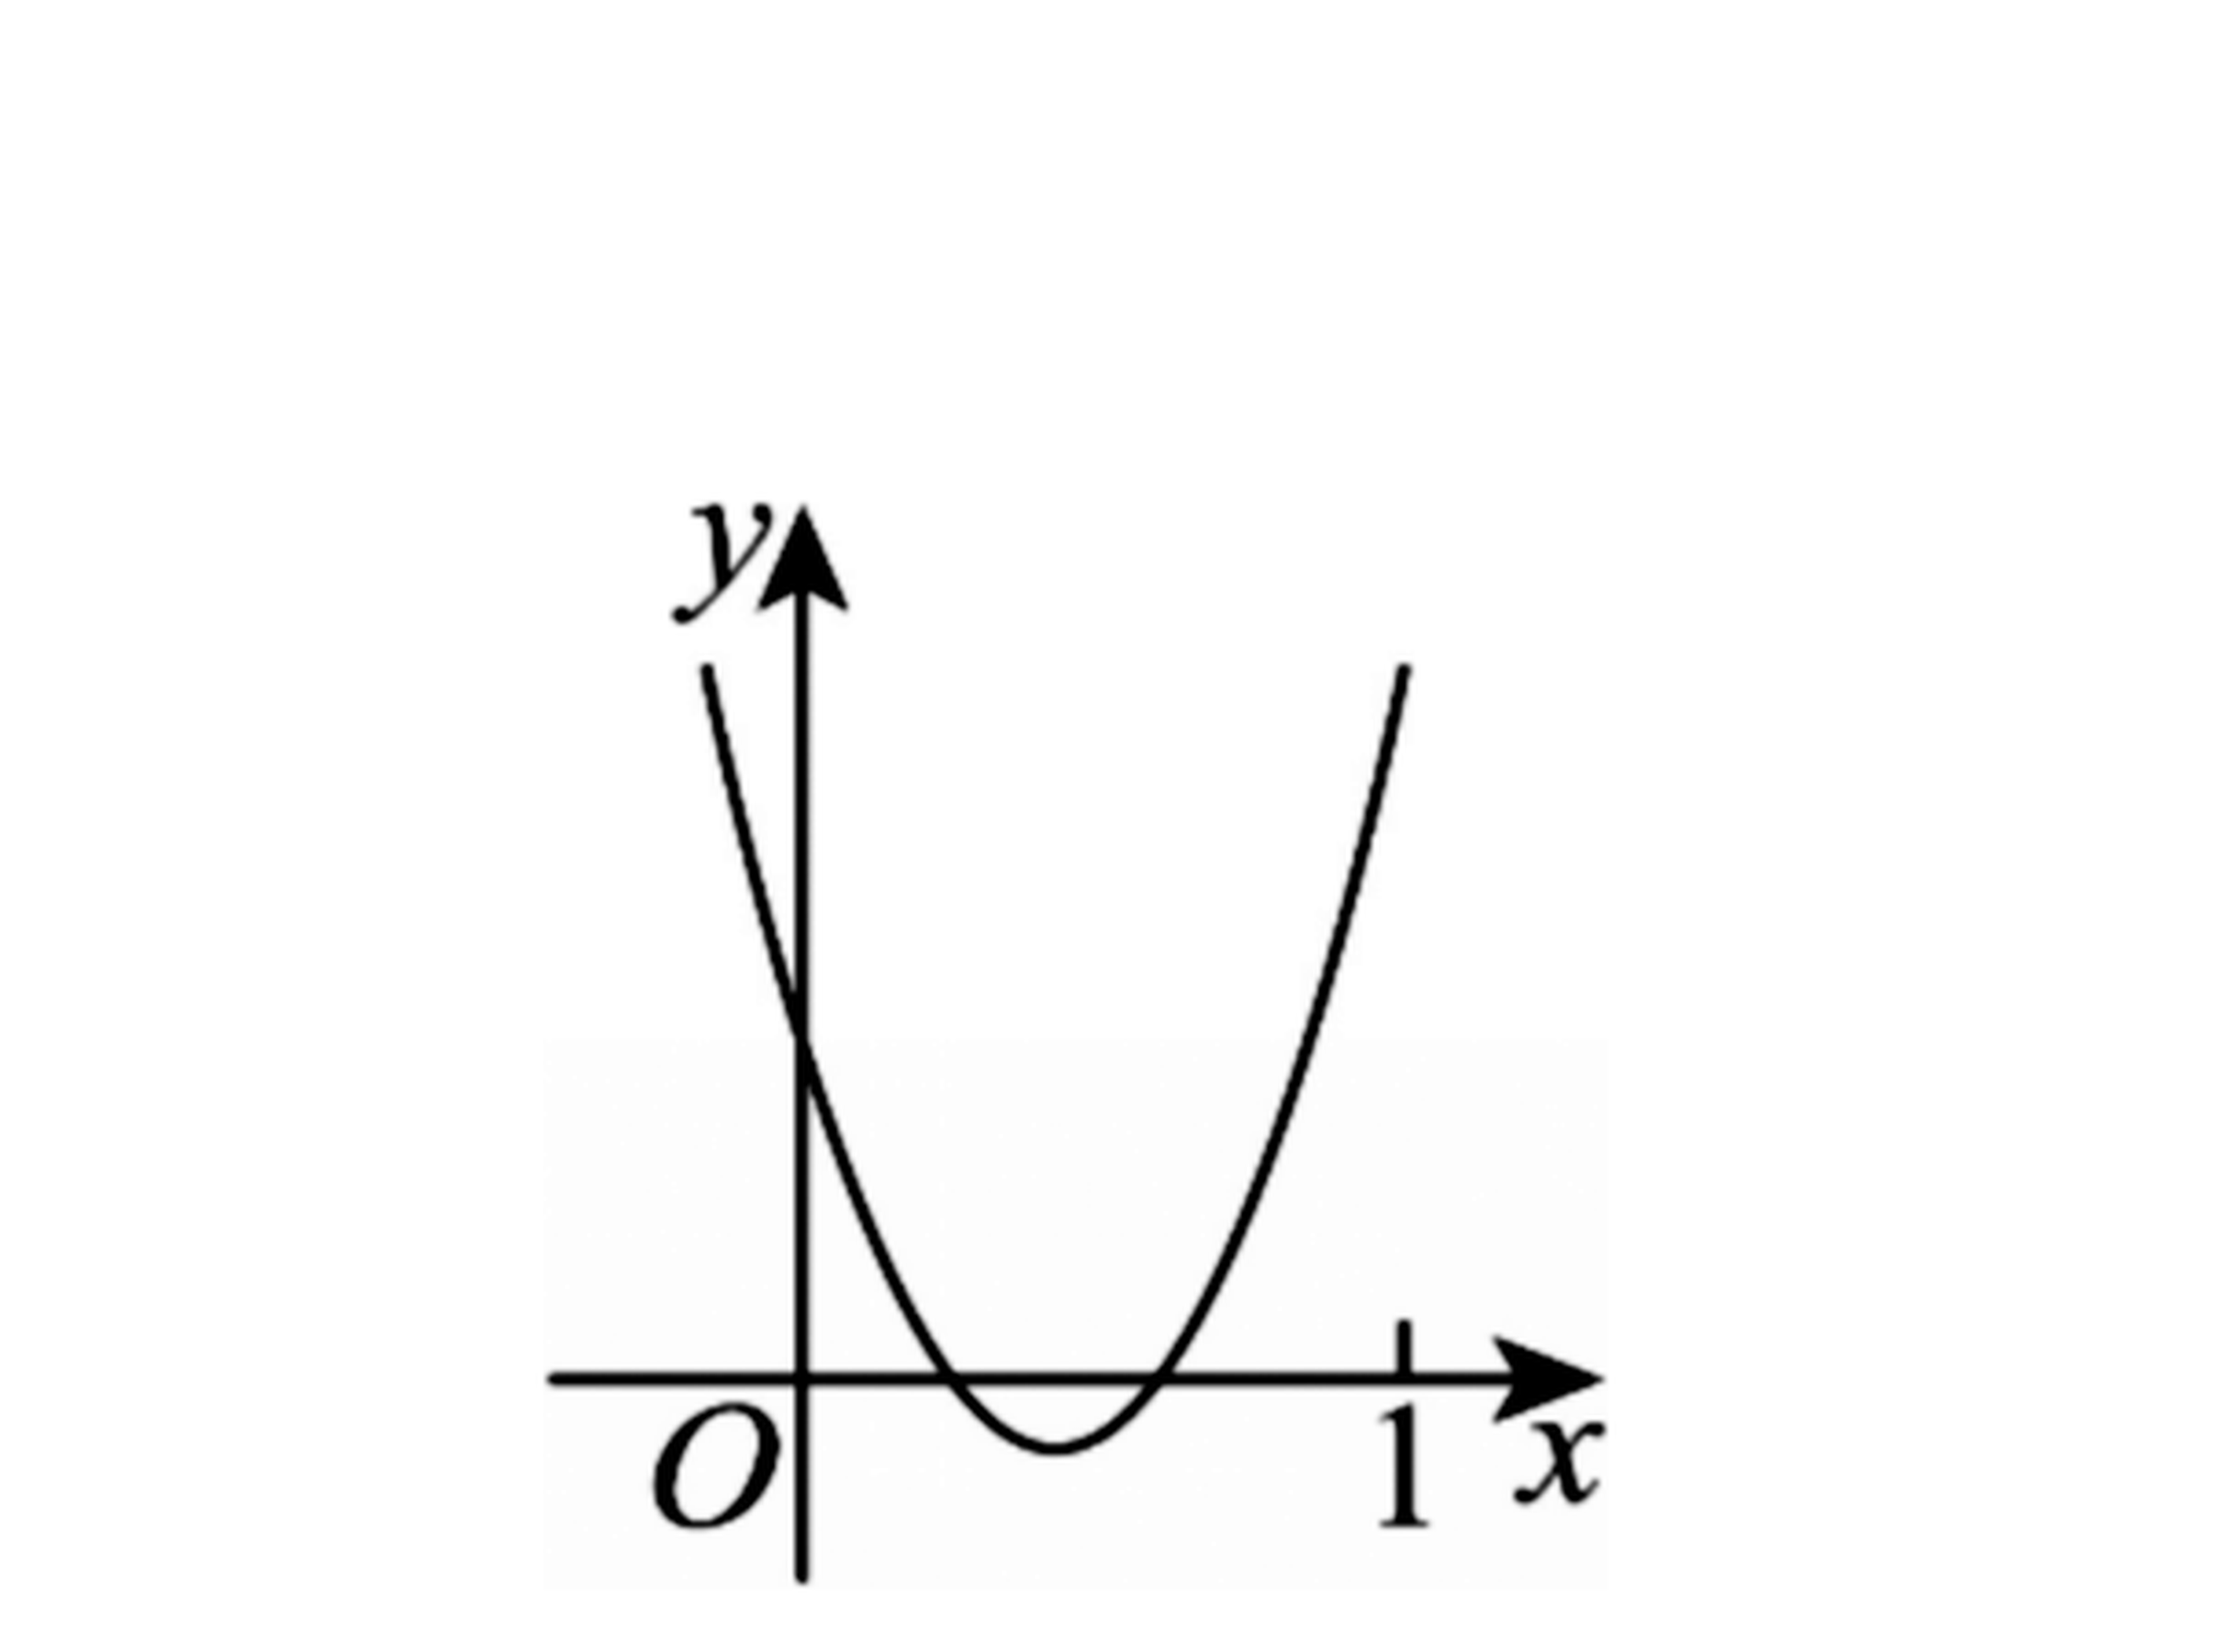
\includegraphics[width=0.32\textwidth]{figures/gao154_q15_stem.png}
\end{center}

\keepwithprev
\begin{center}
% 四幅指数函数图像选项取 05 页上半，按原卷 2×2 排布合并为一张，去粉色水印、去色、4× LANCZOS 放大；三版都出
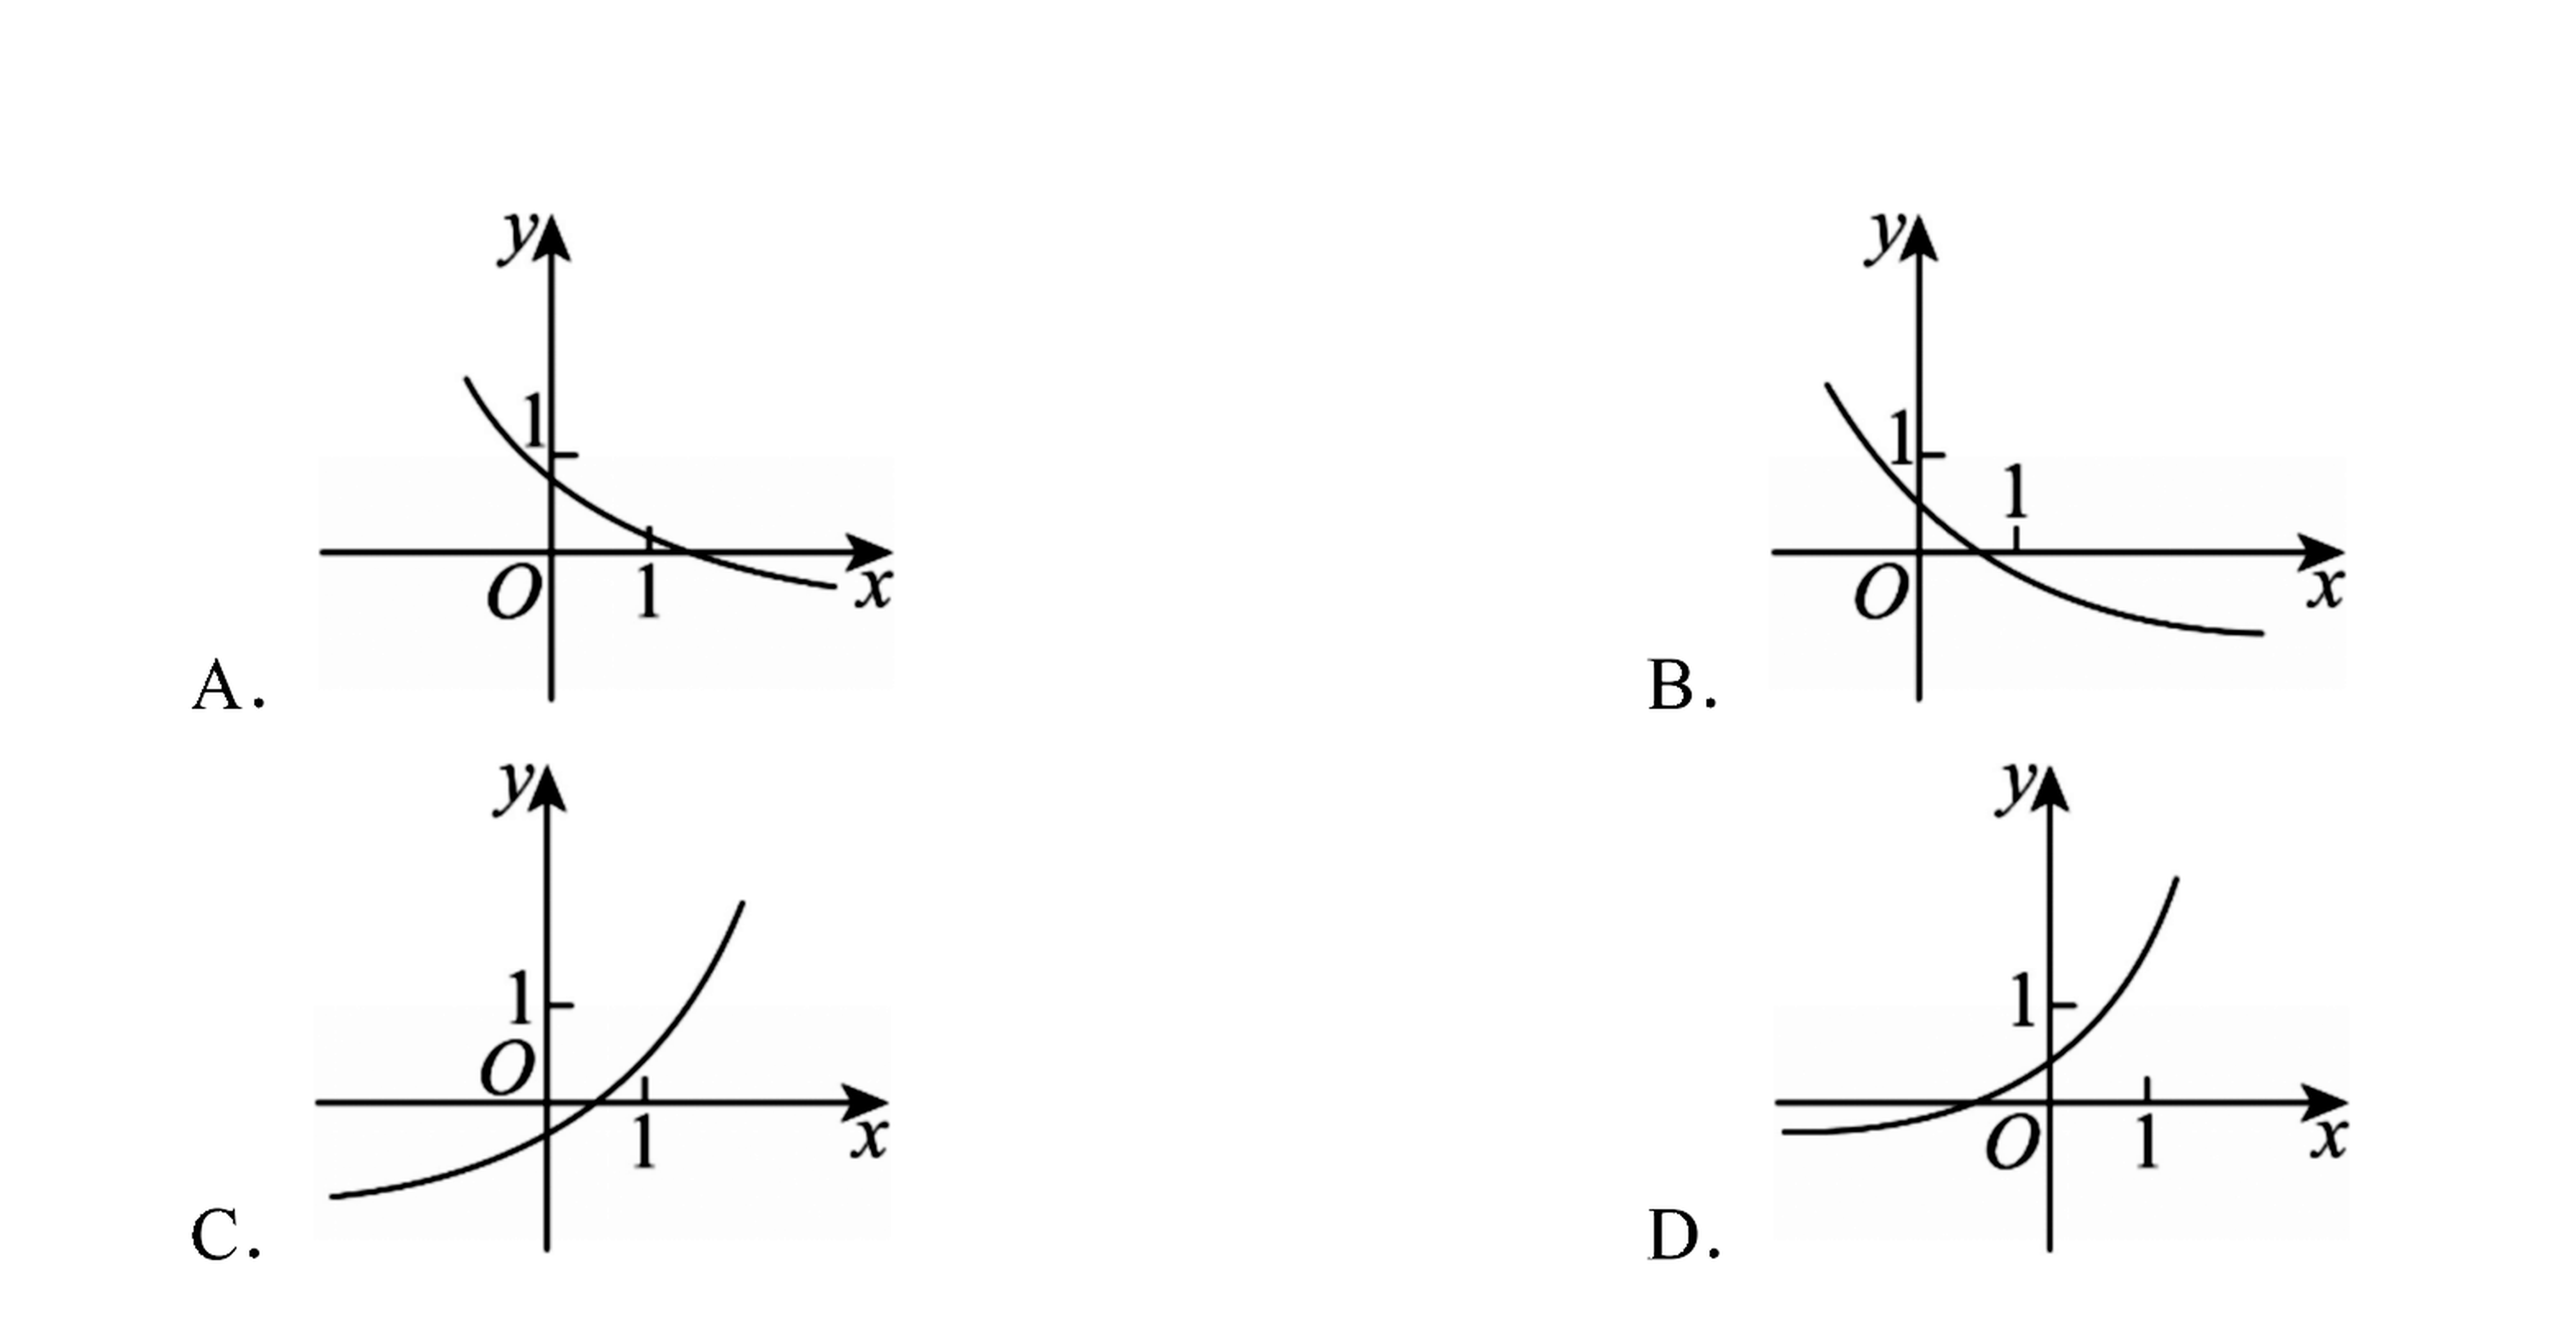
\includegraphics[width=0.80\textwidth]{figures/gao154_q15_opts.png}
\end{center}

\ifanswer
\solbegin
\step{由题意得 $0<a<b<1$，所以 $g(x)=a^x-b$ 在定义域 $\R$ 上严格减.}
\step{$g(0)=a^0-b=1-b>0$，$g(1)=a^1-b=a-b<0$，故 B 符合题意.}
\step{故选 $B$.}
\solend
\fi

% === Q16 === 高斯取整；解析 13 行，故选 C
\item 设 $[a]$ 表示不超过 $a$ 的最大整数，如 $[1.2]=1$，$[-3.2]=-4$，若 $x$、$y$、$z$ 为正实数，则 $\left[\dfrac{y+z}{x}\right]+\left[\dfrac{z+x}{y}\right]+\left[\dfrac{x+y}{z}\right]$ 的最小值为\mbox{（\quad）}

\keepwithprev
A. 2\qquad\qquad B. 3\qquad\qquad C. 4\qquad\qquad D. 6

\ifanswer
\solbegin
\step{若 $x$、$y$、$z$ 为正实数，}
\step{结合基本不等式得 $\dfrac{y+z}{x}+\dfrac{z+x}{y}+\dfrac{x+y}{z}=\dfrac yx+\dfrac xy+\dfrac zx+\dfrac xz+\dfrac zy+\dfrac yz$}
\step{$\geqslant2\sqrt{\dfrac yx\cdot\dfrac xy}+2\sqrt{\dfrac zx\cdot\dfrac xz}+2\sqrt{\dfrac zy\cdot\dfrac yz}=6$，当且仅当 $x=y=z$ 时取等号，}
\step{即 $\dfrac{y+z}{x}$，$\dfrac{z+x}{y}$，$\dfrac{x+y}{z}$ 中至少有一个不小于 2，不妨设 $\dfrac{y+z}{x}\geqslant\dfrac{z+x}{y}\geqslant\dfrac{x+y}{z}$，}
\step{$[a]$ 表示不超过 $a$ 的最大整数和 $\dfrac{y+z}{x}$，$\dfrac{z+x}{y}$，$\dfrac{x+y}{z}$ 中至少有一个不小于 2，}% 原卷此行把两句连写，照录未改（见 ⑤ 3）
\step{得 $\left[\dfrac{y+z}{x}\right]\geqslant2$，所以 $\left[\dfrac{y+z}{x}\right]+\left[\dfrac{z+x}{y}\right]+\left[\dfrac{x+y}{z}\right]\geqslant2$，}
\step{假设 $\left[\dfrac{y+z}{x}\right]+\left[\dfrac{z+x}{y}\right]+\left[\dfrac{x+y}{z}\right]$ 的最小值为 2，$\left[\dfrac{y+z}{x}\right]=2$，$\left[\dfrac{z+x}{y}\right]+\left[\dfrac{x+y}{z}\right]=0$，}
\step{所以 $2\leqslant\dfrac{y+z}{x}<3$，$0<\dfrac{z+x}{y}<1$，$0<\dfrac{x+y}{z}<1$，所以 $2<\dfrac{y+z}{x}+\dfrac{z+x}{y}+\dfrac{x+y}{z}<5$，}
\step{与 $\dfrac{y+z}{x}+\dfrac{z+x}{y}+\dfrac{x+y}{z}\geqslant6$ 矛盾，假设不成立，A 错误；}
\step{假设 $\left[\dfrac{y+z}{x}\right]+\left[\dfrac{z+x}{y}\right]+\left[\dfrac{x+y}{z}\right]$ 的最小值为 3，}
\step{则 $\left[\dfrac{y+z}{x}\right]=2$，$\left[\dfrac{z+x}{y}\right]=1$，$\left[\dfrac{x+y}{z}\right]=0$ 或 $\left[\dfrac{y+z}{x}\right]=3$，$\left[\dfrac{z+x}{y}\right]=\left[\dfrac{x+y}{z}\right]=0$，}
\step{同理可得 $3<\dfrac{y+z}{x}+\dfrac{z+x}{y}+\dfrac{x+y}{z}<6$，显然不成立，B 错误；}
\step{假设 $\left[\dfrac{y+z}{x}\right]+\left[\dfrac{z+x}{y}\right]+\left[\dfrac{x+y}{z}\right]$ 的最小值为 4，易得 $4<\dfrac{y+z}{x}+\dfrac{z+x}{y}+\dfrac{x+y}{z}<7$，}
\step{若取 $x=100$，$y=103$，$z=104$，则 $\left[\dfrac{y+z}{x}\right]=2$，$\left[\dfrac{z+x}{y}\right]=1$，$\left[\dfrac{x+y}{z}\right]=1$，}
\step{即 $\left[\dfrac{y+z}{x}\right]+\left[\dfrac{z+x}{y}\right]+\left[\dfrac{x+y}{z}\right]=4$，假设成立，C 正确，D 错误.}
\step{故选 $C$.}
\solend
\fi

\end{enumerate}

\bigsec{三、解答题}

\begin{enumerate}
\setcounter{enumi}{16}

% === Q17 === $B\subset A$ 单线照录；cases 块；解析 5 行
\item 设集合 $A=\{x\mid x^2+2x-3<0\}$，集合 $B=\{x\mid\lvert x+a\rvert<1\}$.

(1) 若 $a=3$，求 $A\cup B$；

(2) 设命题 $p:x\in A$，命题 $q:x\in B$，若 $p$ 是 $q$ 成立的必要不充分条件，求实数 $a$ 的取值范围.

\ifanswer
\solbegin
\step{(1) $A=(-3,1)$，}
\step{当 $a=3$ 时，$\lvert x+3\rvert<1$，解得 $-4<x<-2$，所以 $B=(-4,-2)$，}
\step{所以 $A\cup B=(-4,1)$.}
\step{(2) 因为 $p$ 是 $q$ 成立的必要不充分条件，所以 $B\subset A$.}
\step{因为 $A=(-3,1)$，$B=(-a-1,-a+1)$，所以 $\begin{cases}-a-1\geqslant-3\\-a+1<1\end{cases}$ 或 $\begin{cases}-a-1>-3\\-a+1\leqslant1\end{cases}$，解得 $0\leqslant a\leqslant2$.}
\solend
\fi

% === Q18 === 判别式 \Delta 两处照录；解析 9 行
\item 已知关于 $x$ 的一元二次方程 $x^2-mx+4m^2-3=0$ 的两个实根分别为 $x_1,x_2$.

(1) 若 $x_1,x_2$ 满足 $x_1+x_2=x_1x_2$，求实数 $m$ 的值；

(2) 求 $x_1^2+x_2^2$ 的最小值.

\ifanswer
\solbegin
\step{(1) 由韦达定理 $x_1+x_2=m$，$x_1x_2=4m^2-3$，}
\step{$\Delta=m^2-4(4m^2-3)=-15m^2+12\geqslant0$，即 $m^2\leqslant\dfrac45$.}
\step{由 $x_1+x_2=x_1x_2$ 得 $m=4m^2-3$，即 $4m^2-m-3=0$，}
\step{解得 $m=1$ 或 $m=-\dfrac34$.}
\step{$m=1$ 时 $m^2=1>\dfrac45$，$\Delta<0$，舍去；}
\step{$m=-\dfrac34$ 时 $m^2=\dfrac9{16}<\dfrac45$，符合，故 $m=-\dfrac34$.}
\step{(2) $x_1^2+x_2^2=(x_1+x_2)^2-2x_1x_2=m^2-2(4m^2-3)=-7m^2+6$，}
\step{函数 $y=-7m^2+6$ 开口向下，对称轴为 $m=0$，}% 原卷此处称求「最小值」，实为闭区间 $m^2\le\frac45$ 上的最小值，照录未改（见 ⑤ 4）
\step{故 $y_{\min}=-7\cdot\dfrac45+6=-\dfrac{28}{5}+\dfrac{30}{5}=\dfrac25$.}
\solend
\fi

% === Q19 === 全称命题；cases 块；解析 9 行
\item 设命题 $p$：对任意 $x\in\R$，不等式 $2mx^2+2mx+1>0$ 恒成立，$q:m\in\{m\mid\log_2(m-1)<1\}$.

(1) 若 $p$ 为真命题，求实数 $m$ 的取值范围；

(2) 若命题 $p$、$q$ 有且只有一个是真命题，求实数 $m$ 的取值范围.

\ifanswer
\solbegin
\step{(1) 由 $p$ 为真命题，得 $\forall x\in\R$，不等式 $2mx^2+2mx+1>0$ 恒成立，}
\step{当 $m=0$ 时，$1>0$ 恒成立；}
\step{当 $m\ne0$ 时，$\begin{cases}2m>0\\\Delta=4m^2-8m<0\end{cases}$，解得 $0<m<2$；}
\step{综上，$0\leqslant m<2$，即 $m$ 的取值范围是 $[0,2)$；}
\step{(2) 若 $q$ 为真，则有 $\log_2(m-1)<1$，得 $0<m-1<2$，解得 $1<m<3$，}
\step{因此命题 $q:m\in\{m\mid1<m<3\}$，由 (1) 得命题 $p:\{m\mid0\leqslant m<2\}$，}
\step{而命题 $p$、$q$ 有且只有一个是真命题，}
\step{当 $p$ 真 $q$ 假时，$\begin{cases}0\leqslant m<2\\m\leqslant1\text{ 或 }m\geqslant3\end{cases}$，解得 $0\leqslant m\leqslant1$，}
\step{当 $p$ 假 $q$ 真时，$\begin{cases}m<0\text{ 或 }m\geqslant2\\1<m<3\end{cases}$，解得 $2\leqslant m<3$，}
\step{故实数 $m$ 的取值范围是 $\{m\mid0\leqslant m\leqslant1\text{ 或 }2\leqslant m<3\}$.}
\solend
\fi

% === Q20 === Labubu 成本题；解析 10 行
\item Labubu 公司拟在 2027 年初推出智能机器人系列玩偶（单位：套）. 根据以往经验，其中一条生产线每月生产 $x$ 套玩具的成本 $P$ 由两部分费用（单位：元）构成：

(i) 固定成本（与生产玩具套数 $x$ 无关），总计 160000 元；

(ii) 每生产 $x$ 套需另投入的生产成本 $c(x)$ 元，其中 $c(x)=10x+\dfrac1{100}x^2$.

(1) 假设该生产线每月生产出的玩具能全部售出，问：该生产线每月生产玩具多少套时，可使得平均每套所需成本费用最少？此时每套玩具的成本费用是多少？

(2) 假设该生产线每月生产出的玩具能全部售出，但随着 $x$ 的增大，每月生产所需的直接总成本在急剧增加，因此售价也需随着 $x$ 的增大而适当增加. 设每套玩具的售价为 $q(x)$ 元，$q(x)=a+\dfrac xb$（$a,b\in\R$）. 若当月产量为 10000 套时利润最大，此时每套售价为 150 元，试求 $a,b$ 的值.（利润=销售收入$-$成本费用）

\ifanswer
\solbegin
\step{(1) 每月总成本 $P=160000+10x+\dfrac1{100}x^2$，}
\step{平均每套成本为 $\dfrac Px=\dfrac{160000}{x}+10+\dfrac x{100}\geqslant10+2\sqrt{\dfrac{160000}{x}\cdot\dfrac x{100}}=90$.}
\step{等号成立当且仅当 $\dfrac{160000}{x}=\dfrac x{100}$ 时，即 $x=4000$ 时取等号，}
\step{所以每月生产 4000 套时平均每套成本最少，此时每套成本为 90 元.}
\step{(2) 利润 $W(x)=x\cdot q(x)-P=\left(\dfrac1b-\dfrac1{100}\right)x^2+(a-10)x-160000$.}
\step{要在 $x=10000$ 处取得最大值，需 $\dfrac1b-\dfrac1{100}<0$，且对称轴为 $x=10000$，}
\step{故 $-\dfrac{a-10}{2\left(\frac1b-\frac1{100}\right)}=10000$，即 $a-10=-20000\left(\dfrac1b-\dfrac1{100}\right)$.}
\step{又 $q(10000)=a+\dfrac{10000}{b}=150$.}
\step{令 $t=\dfrac1b$，则 $a=150-10000t$，}
\step{代入上式 $140-10000t=-20000t+200$，解得 $t=\dfrac3{500}$，即 $b=\dfrac{500}{3}$；}
\step{再由 $a=150-10000\times\dfrac3{500}=150-60=90$，所以 $a=90$，$b=\dfrac{500}{3}$.}
\solend
\fi

% === Q21 === $A^+$／$A^-$ 新定义；$A\subseteq$ 带下划线照录、\varnothing；解析 16 行
\item 设集合 $A$ 为非空数集，定义 $A^+=\{x\mid x=a+b,a,b\in A\}$，$A^-=\{x\mid x=\lvert a-b\rvert,a,b\in A\}$.

(1) 若集合 $A=\{-1,1\}$，写出集合 $A^+$ 及 $A^-$；

(2) 若集合 $A=\{x_1,x_2,x_3,x_4\}$，$x_1<x_2<x_3<x_4$，且 $A^-=A$，求证：$x_1+x_4=x_2+x_3$；

(3) 若集合 $A\subseteq\{x\mid0\leqslant x\leqslant2020,x\in\N\}$，且 $A^+\cap A^-=\varnothing$，求集合 $A$ 元素的个数的最大值.

\ifanswer
\solbegin
\step{(1) 由 $A=\{-1,1\}$，得 $A^+=\{-2,0,2\}$，$A^-=\{0,2\}$；}
\step{(2) 由于集合 $A=\{x_1,x_2,x_3,x_4\}$，$x_1<x_2<x_3<x_4$，且 $A^-=A$，}
\step{所以 $A^-$ 中也只包含四个元素，即 $A^-=\{0,x_2-x_1,x_3-x_1,x_4-x_1\}$，}
\step{剩下的 $x_3-x_2=x_4-x_3=x_2-x_1$，所以 $x_1+x_4=x_2+x_3$；}
\step{(3) 设 $A=\{a_1,a_2,\cdots,a_k\}$ 满足题意，其中 $a_1<a_2<\cdots<a_k$，}
\step{则 $2a_1<a_1+a_2<a_1+a_3<\cdots<a_1+a_k<a_2+a_k<a_3+a_k<\cdots<a_{k-1}+a_k<2a_k$，所以 $\lvert A^+\rvert\geqslant2k-1$，}
\step{且 $a_1-a_1<a_2-a_1<a_3-a_1<\cdots<a_k-a_1$，所以 $\lvert A^-\rvert\geqslant k$，}
\step{因为 $A^+\cap A^-=\varnothing$，所以 $\lvert A^+\cup A^-\rvert=\lvert A^+\rvert+\lvert A^-\rvert\geqslant3k-1$，}
\step{$A^+\cup A^-$ 中最小的元素为 0，最大的元素为 $2a_k$，所以 $\lvert A^+\cup A^-\rvert\leqslant2a_k+1$，}
\step{所以 $3k-1\leqslant2a_k+1\leqslant4041$（$k\in\N^*$），所以 $k\leqslant1347$，}
\step{实际上当 $A=\{674,675,676,\cdots,2020\}$ 时满足题意，证明如下：}
\step{设 $A=\{m,m+1,m+2,\cdots,2020\}$，$m\in\N$，}
\step{则 $A^+=\{2m,2m+1,2m+2,\cdots,4040\}$，$A^-=\{0,1,2,\cdots,2020-m\}$，}
\step{由题意得 $2020-m<2m$，即 $m>673\dfrac13$，}
\step{故 $m$ 的最小值为 674，于是当 $m=674$ 时，$A$ 中元素最多，}
\step{即 $A=\{674,675,676,\cdots,2020\}$ 时满足题意，}
\step{综上所述，集合 $A$ 中元素的个数的最大值是 1347.}
\solend
\fi

\end{enumerate}

\bigsec{附加题}

\begin{enumerate}

% === 附加题 1 === 另起编号 1；「n 元集和集」弯引号；解析 6 行
\item 设集合 $A=\{a_1,a_2,a_3,a_4\}$，$C=\{2,3,4,6\}$，新定义：集合 $A$ 中所有含 $n$ 个元素的子集中 $n$ 个元素之和的不同值组成的集合为“$n$ 元集和集”. 若 $A$ 的“3 元集和集”为 $C$，则集合 $A=$\blankline[4.4em].

\ifanswer
\solbegin
\step{集合 $A$ 的 3 元子集共有 4 个：$\{a_1,a_2,a_3\}$，$\{a_1,a_2,a_4\}$，$\{a_1,a_3,a_4\}$，$\{a_2,a_3,a_4\}$，}
\step{集合 $C=\{a_1+a_2+a_3,a_1+a_2+a_4,a_1+a_3+a_4,a_2+a_3+a_4\}$，}
\step{不妨令 $a_1<a_2<a_3<a_4$，}
\step{则 $a_1+a_2+a_3<a_1+a_2+a_4<a_1+a_3+a_4<a_2+a_3+a_4$，}
\step{而 $C=\{2,3,4,6\}$，因此 $\begin{cases}a_1+a_2+a_3=2\\a_1+a_2+a_4=3\\a_1+a_3+a_4=4\\a_2+a_3+a_4=6\end{cases}$，相加化简得 $a_1+a_2+a_3+a_4=5$，}
\step{解得 $a_1=-1$，$a_2=1$，$a_3=2$，$a_4=3$，所以 $A=\{-1,1,2,3\}$.}
\solend
\fi

% === 附加题 2 === 解析配图（仅答案版出）；四选项；解析 15 行，故选 A
\item 已知函数 $f(x)=\log_p x+q$，其中 $p>0$ 且 $p\ne1$，曲线 $y=f(x)$ 经过 $P(1,2)$、$Q(2,3)$ 两点. 设 $g(x)=f(x)\cdot[f(x)-2]$，若 $\lvert g(a)\rvert=\lvert g(b)\rvert=\lvert g(c)\rvert=\lvert g(d)\rvert$，且 $a<b<c<d$，则 $ad(b+c)$ 的取值范围为\mbox{（\quad）}

\keepwithprev
A. $\left(\dfrac14,\dfrac5{16}\right)$\qquad B. $\left(\dfrac18,\dfrac5{16}\right)$\qquad C. $\left(\dfrac14,\dfrac25\right)$\qquad D. $\left(\dfrac18,\dfrac25\right)$

\ifanswer
\solbegin
\step{函数 $f(x)=\log_p x+q$，且曲线 $y=f(x)$ 经过点 $P(1,2)$ 和 $Q(2,3)$，}
\step{所以 $\begin{cases}f(1)=q=2\\f(2)=\log_p2+q=3\end{cases}$，解得 $p=2$，$q=2$，$f(x)=\log_2 x+2$.}
\step{不妨设 $\lvert g(x)\rvert=k$，令 $\log_2 x=m$，则 $f(x)\cdot[f(x)-2]=m(m+2)=m^2+2m$，}
\step{画出函数 $y=\lvert m^2+2m\rvert$ 的图象，如图所示，}
\begin{center}
% $y=|m(m+2)|$ 图像取 11 页右上，去粉色水印、去色、4× LANCZOS 放大；仅答案版出
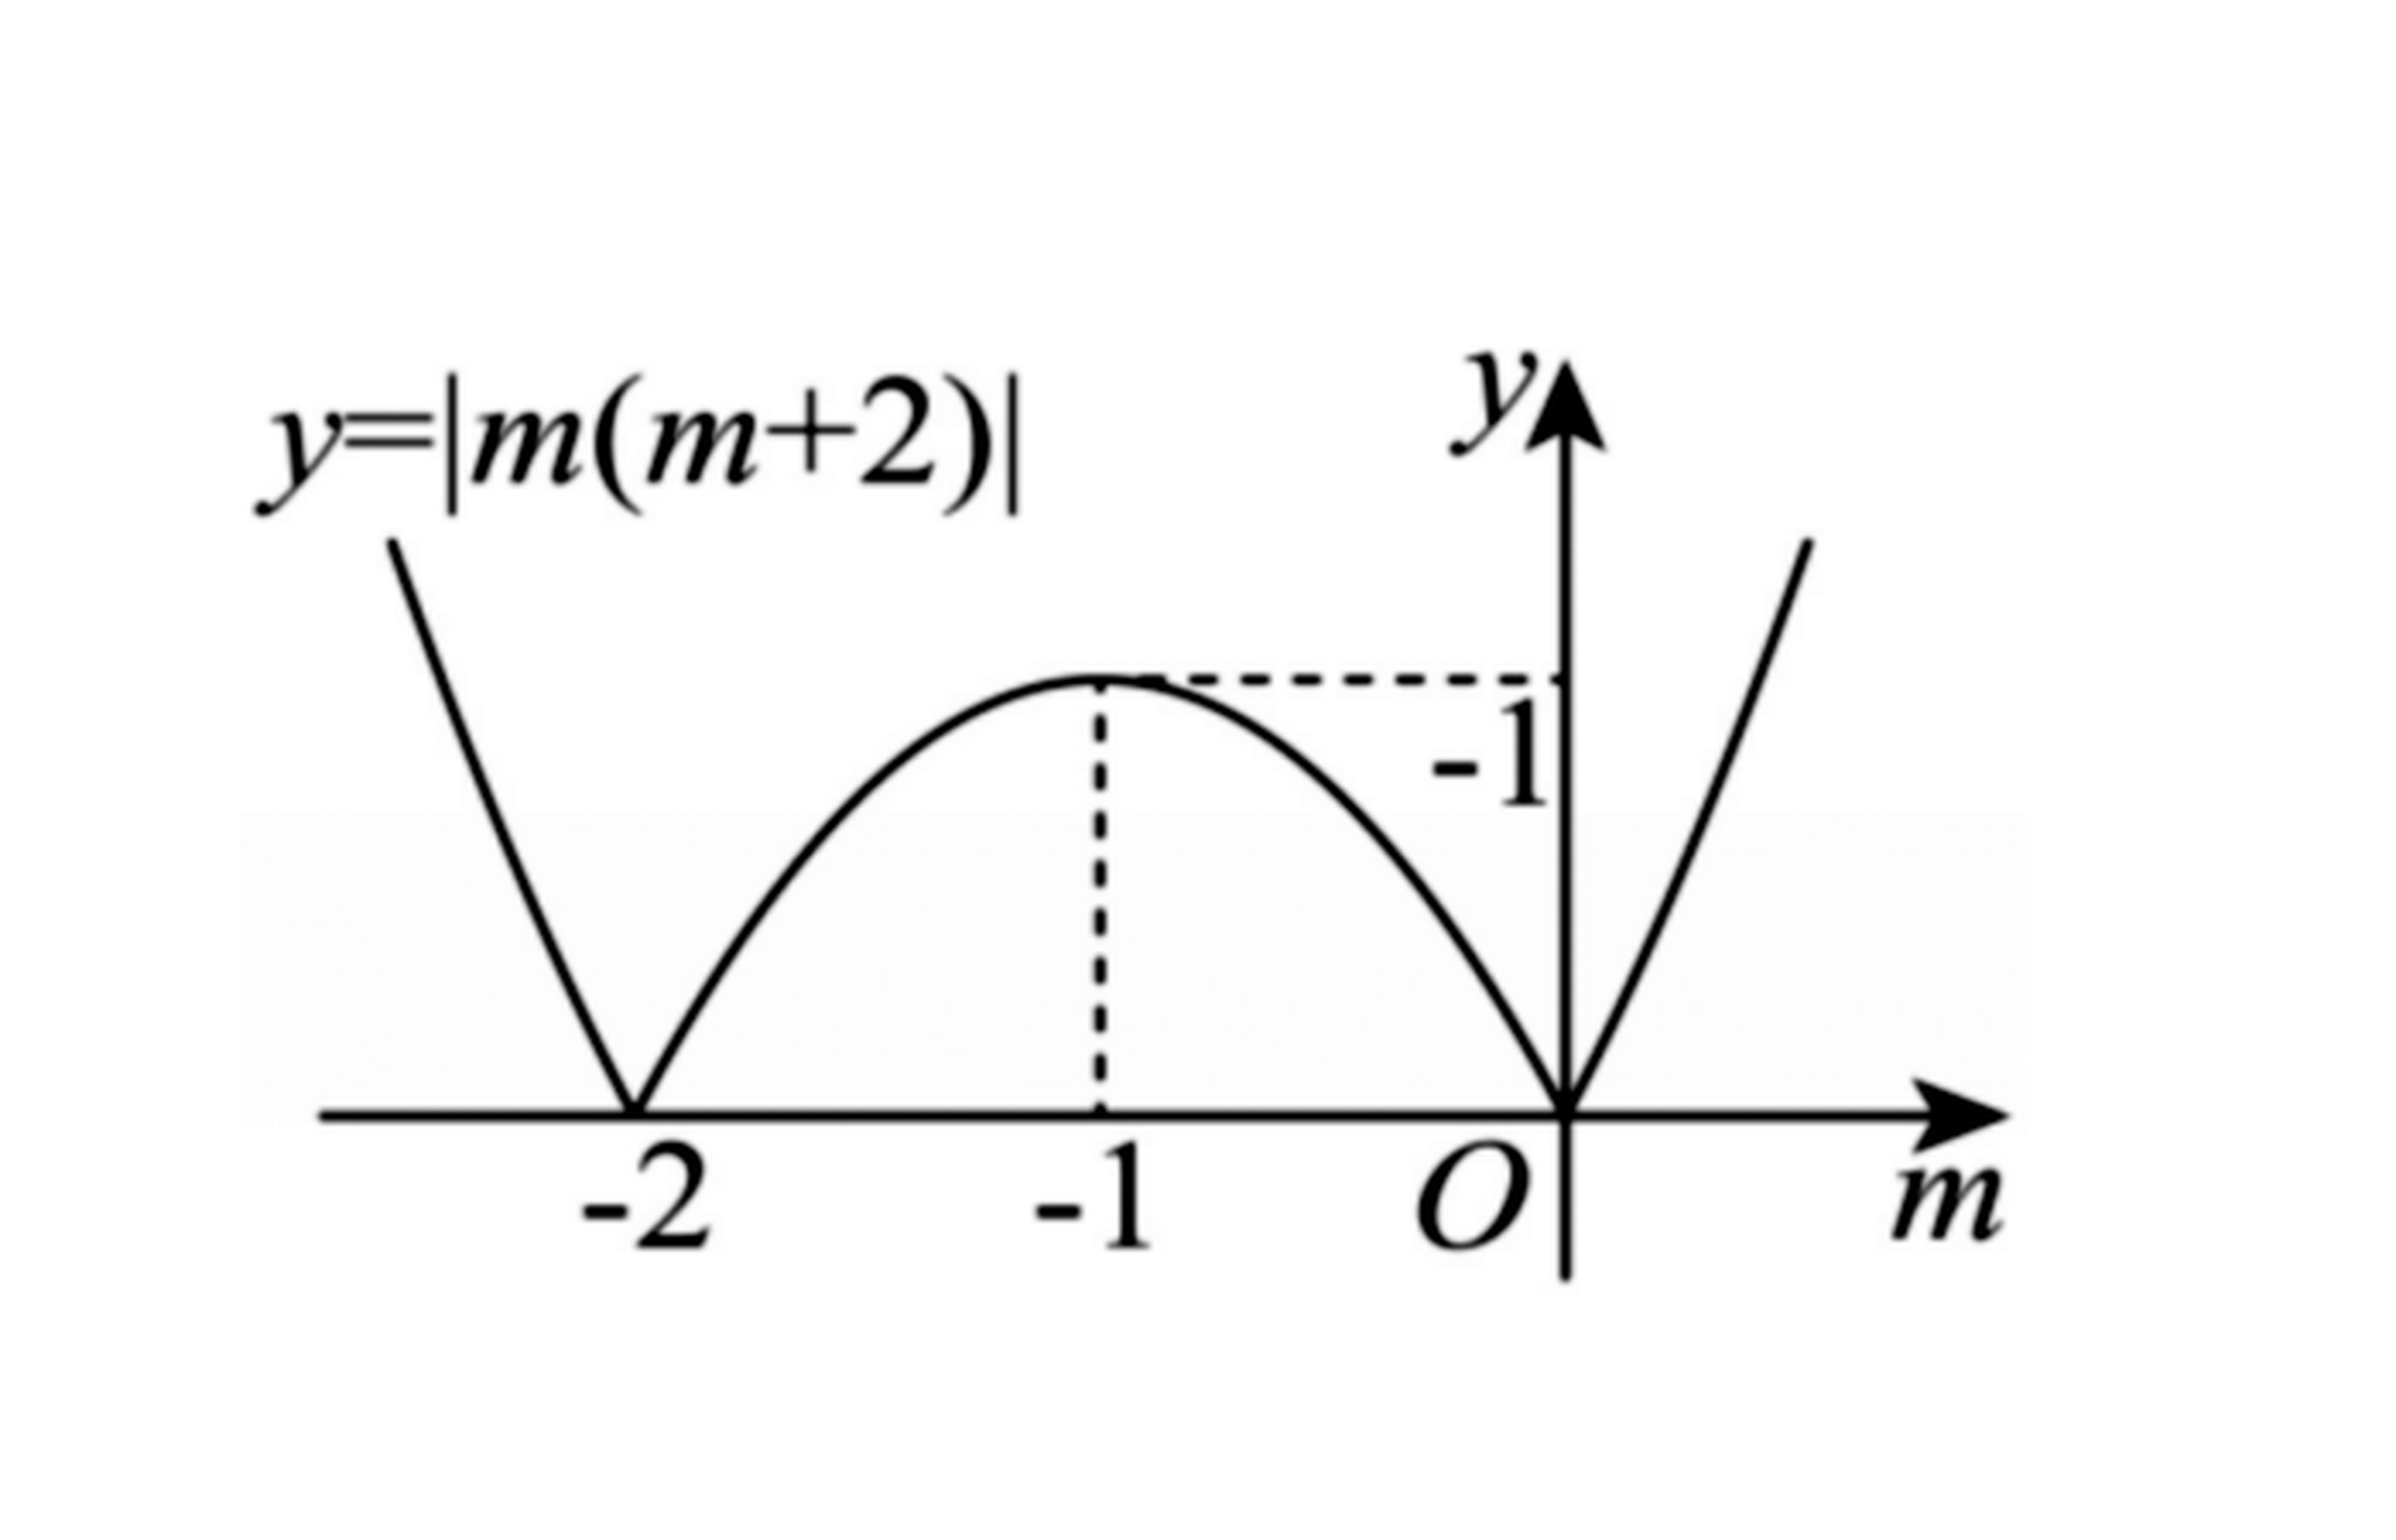
\includegraphics[width=0.46\textwidth]{figures/gao154_fujia2.png}
\end{center}
\step{由图像得 $k\in(0,1)$，}
\step{所以方程 $m^2+2m=k$ 和 $m^2+2m=-k$ 各有两个不同的根，}
\step{其中方程 $m^2+2m-k=0$ 的两根为 $m=-1\pm\sqrt{1+k}$，}
\step{方程 $m^2+2m+k=0$ 的两根为 $m=-1\pm\sqrt{1-k}$，}
\step{所以 $m_1=-1-\sqrt{1+k}$，$m_2=-1-\sqrt{1-k}$，$m_3=-1+\sqrt{1-k}$，$m_4=-1+\sqrt{1+k}$，且 $m_1<m_2<m_3<m_4$，}
\step{由 $m=\log_2 x$，则 $x=2^m$，}
\step{所以 $a=2^{-1-\sqrt{1+k}}$，$b=2^{-1-\sqrt{1-k}}$，$c=2^{-1+\sqrt{1-k}}$，$d=2^{-1+\sqrt{1+k}}$，}
\step{所以 $ad=2^{-1-\sqrt{1+k}}\times2^{-1+\sqrt{1+k}}=2^{(-1-\sqrt{1+k})+(-1+\sqrt{1+k})}=2^{-2}=\dfrac14$，}
\step{$b+c=2^{-1-\sqrt{1-k}}+2^{-1+\sqrt{1-k}}=\dfrac{2^{-\sqrt{1-k}}+2^{\sqrt{1-k}}}{2}$，}
\step{令 $s=\sqrt{1-k}$，其中 $s\in(0,1)$，则 $b+c=\dfrac12\left(2^{-s}+2^s\right)$，}
\step{设函数 $y=2^s+\dfrac1{2^s}$，令 $r=2^s\in(1,2)$，所以 $y=r+\dfrac1r$ 在 $(1,2)$ 上严格增，}
\step{所以函数 $y=2^s+\dfrac1{2^s}$ 在 $(0,1)$ 上严格增，所以 $y=2^s+\dfrac1{2^s}\in\left(2,\dfrac52\right)$，}
\step{所以 $b+c=\dfrac{2^{-s}+2^s}{2}\in\left(1,\dfrac54\right)$，$ad(b+c)=\dfrac{b+c}{4}\in\left(\dfrac14,\dfrac5{16}\right)$，}
\step{所以 $ad(b+c)$ 的取值范围是 $\left(\dfrac14,\dfrac5{16}\right)$，故选 $A$.}
\solend
\fi

\end{enumerate}

\end{document}
"
% 紧凑版：xelatex "\def\iscompact{1}% 高一154_徐汇中学_期中.tex
%   —— 高一上数学"2026-2027 年徐汇中学高一上期中"（试卷版/答案版/紧凑版）
% 试卷版：xelatex 高一154_徐汇中学_期中.tex
% 答案版：xelatex "\def\isanswer{1}\input{高一154_徐汇中学_期中.tex}"
% 紧凑版：xelatex "\def\iscompact{1}\input{高一154_徐汇中学_期中.tex}"
%
% ① 原始材料：微信公众号"魔都数学加油站"文章，连载"27学年高一154"，原文标题
% "27学年高一154——2026-2027年上海市徐汇中学高一上期中"；
% 原文链接：https://mp.weixin.qq.com/s/Qs2T7Zwsug-KKFE2wefDUg 。
% 正文为 12 张 PNG 页（01/03/04/05/07/11/12 为 2560×3620，
% 02/06/08/09/10 为 4762×6735，同一篇各页分辨率混排，逐页按各自分辨率裁图核对）。
% 体例：讲评版——一、填空题 3—12（10 题）、二、选择题 13—16（4 题）、
% 三、解答题 17—21（5 题）、附加题 1—2（2 题，原卷**另起编号**"1." "2."，
% 不与正题连号，同 高一a 成例），共 21 题；全卷每题均印【解析】
% （逐题核实，见 ② ②）。题目、答案、解析均据原图转录；卷面粉红色水印
% "魔都数学加油站"及公众号页脚未录入。
% 全卷插图清单（逐页通读 12 页确认）：3 组——
%   · Q15 题干配图（$f(x)=(x-a)(x-b)$ 抛物线，04 页右下：x/y 轴、O、1、
%     开口向上两零点均在 (0,1) 内），三版都出，裁 figures/gao154_q15_stem.png；
%   · Q15 四幅图像选项（05 页上半 2×2 排布，A/B/C/D 四幅指数函数图像，
%     合并成一张，照 高一136 Q13/Q22 成例），三版都出，
%     裁 figures/gao154_q15_opts.png；
%   · 附加题第 2 题解析配图（$y=\lvert m(m+2)\rvert$ 图像，11 页右上：
%     W 形折线、$-2$、$-1$、O、虚线 $y=1$ 与 $m=-1$），仅答案版出，
%     裁 figures/gao154_fujia2.png；
%   3 图均取自原卷截图，去粉色水印、去色、4× LANCZOS 放大；Q15 题干图
%   左侧题干残字"的图"已裁白。其余各页逐页确认无其它题目配图、无表格；
%   12 页下半仅水印、无正文。
%
% 卷首标题：原卷印作"2026-2027 年徐汇中学高一上期中"，年份区间按全稿惯例排 en dash；
% 原卷卷面未印副标题，本稿按同期中卷知识模块口径补出"集合与常用逻辑用语、不等式、函数"。
%
% ② 与原卷的排版差异：
%   ① 原文从第 3 题起，本稿保留原题号；共 21 题四节，正题到 21，附加题另起编号
%      1—2（\bigsec{附加题} 后 \begin{enumerate} 不 \setcounter，同 高一a 成例）；
%   ② 全 21 题均印【解析】、用 \solbegin…\solend，无只印【答案】或答案印括号内的题；
%      四道正题选择题答案在解析末句"故选 C／A／B／C"（Q13—Q16）、附加题第 2 题
%      答案在解析末句"故选 A"，括号 \mbox{（\quad）} 留空、不另提 \ans{}；
%      答案版【答案】/【解析】标记数 = 21 = 全卷题数；
%   ③ 原卷卷面未印副标题，本稿按知识模块口径补出；
%   ④ 原卷填空横线按全稿惯例排 \blankline[4.4em]；选择题括号排 \mbox{（\quad）}、
%      四道正题选择题与附加题第 2 题的选项段前按惯例各加 \keepwithprev
%      （Q15 与附加题 2 的选项段是整块图，\keepwithprev 后接 \begin{center}）；
%      解答题不留作答区、不加 \anspace（原卷为讲评版）；
%   ⑤ 数集黑板粗体：Q4"$x,y\in R$"、Q9"$x\in\R$"、Q13 无、
%      Q15"定义域 $\R$"、Q19"$\forall x\in\R$"、Q21"$x\in\N$"与"$k\in\N^*$"、
%      Q20"$a,b\in\R$"、附加题 2 无——原卷印斜体或正体粗体 R/N/N*，
%      按全稿惯例归一 \R／\N／\N^*；绝对值排 \lvert…\rvert
%      （Q5、Q9、Q12、Q13、Q16、Q21、附加题 2），集合描述竖线排 \mid
%      （Q5、Q17、Q19、Q21），不等号按全稿惯例排 \leqslant／\geqslant；
%      空集 \varnothing（Q21 题干 (3)）；
%   ⑥ 子集符号逐处照录、不得统一：Q6 题干印"$\{1,2\}\subset M\subseteq\{1,2,3,4,5\}$"
%      （前单线 ⊂、后带下划线 ⊆，同句两形并用），解析亦两形并用；
%      Q17 解析 (2)"$B\subset A$"印单线 ⊂；Q21 题干 (3)"$A\subseteq\{x\mid\cdots\}$"
%      印带下划线 ⊆——逐处放大核，分别 \subset／\subseteq，照录未统一（见 ④）；
%   ⑦ 判别式 Δ/△：Q18 解析 (1)"$\Delta=m^2-4(4m^2-3)$"与 Q19 解析 (1)
%      "$\Delta=4m^2-8m<0$"两处均印等腰偏高粗三角、照录 \Delta；本卷无扁等边
%      细线 \triangle 用例（见 ④）；
%   ⑧ 中文弯引号照录：Q4"设 $x$、$y\in\R$. 若 $x+y>2$，则 $x>1$ 或 $y>1$"、
%      附加题 1"$n$ 元集和集"与"3 元集和集"；注释里一律 ASCII 引号；
%      数学式内 CJK 用 \text{}（Q5 解集描述"或"、Q19 集合描述的"或"）；
%   ⑨ "图像／图象"逐处放大核：Q15 题干与解析印"图象"（象，无亻）、
%      Q16 无、附加题 2 解析印"图象"与"图像"（"画出函数…的图象"、
%      "由图像得"——两形并用，逐处照录未统一）；Q13/Q14 无数集图像字样；
%      半角逗号在数学组之间是全稿惯例、非笔误，逐处照录（Q3、Q10、Q16、
%      Q18、Q20、Q21 的 $x_1,x_2$ 之类）；行末西文句点 ASCII `.`；
%      行中全角逗号／顿号照录（Q6"3，4，5"、Q20"（单位：元）"、
%      附加题 1"$a_1,a_2,a_3,a_4$"）；
%   ⑩ 复杂式照录别简化：Q3 $a^{\frac{12}{7}}\cdot\left(\frac17\right)^{\frac17}
%      \cdot\sqrt[7]{a^4}$ 与 $7^{-\frac17}a^{\frac{16}{7}}$、Q7 $x^{-m}$、
%      Q8 $\frac{b-2a+2}{2a}$、Q11 $\frac{9+4\sqrt2}{6}$、Q12 $506\frac29$ 与
%      $506\frac49$、Q16 高斯取整 $[a]$、Q20 $c(x)=10x+\frac1{100}x^2$ 与
%      $q(x)=a+\frac xb$、Q21 $A^+$／$A^-$ 与 $|A^+|\geqslant2k-1$、
%      附加题 2 $m=-1\pm\sqrt{1+k}$ 与 $ad(b+c)$；
%      \left…\right 不得拆到不同 $…$ 组（Q5 $\left\{x\mid\cdots\right\}$、
%      Q20 $\left(\frac1b-\frac1{100}\right)$、附加题 2 $\left(\frac14,\frac5{16}\right)$）；
%      cases 块一律 \begin{cases}…\end{cases}；
%   ⑪ 一条 \step = 原卷解析的一个印刷行，cases 块整体算一个印刷行；别并折行、
%      别拆行。Q11 九行、Q12 六行、Q16 十六行、Q20 十一行、Q21 十七行、
%      附加题 2 十八行均按印刷行逐条断，不丢行；
%   ⑫ 配图：Q15 题干小图（三版都出）放 \item 内题干之后 \begin{center}，
%      Q15 四幅选项图（三版都出）放 \keepwithprev 之后的 \begin{center}，
%      Q15 用 \needvspace 守卫把"题干＋两图"整块推走（守卫放 \item 之前，
%      见 高一145 Q14/Q20 与 高一136 Q13 成例）；附加题 2 解析配图（仅答案版出）
%      放 \ifanswer 内 \solbegin…\solend 的 \step 之间（高一73 第 16 题成例）；
%   ⑬ 原卷解析内无红色"法一／法二"之类小标题，故本卷无 \stepm；红色水印
%      "魔都数学加油站"不录入；
%   ⑭ 跨页续印按题合并：见 ⑥；
%
% ③ 行数复核：一条 \step = 原卷解析的一个印刷行，cases 块作一个印刷行计。
%   逐题数（主会话逐页核对定稿）：Q3：1；Q4：1；Q5：3；Q6：4；Q7：3；
%   Q8：1；Q9：5；Q10：4；Q11：9；Q12：6；Q13：5；Q14：4；Q15：3；
%   Q16：16；Q17：5；Q18：9；Q19：10；Q20：11；Q21：17；
%   附加题 1：6；附加题 2：18。
%   合计 141 条 \step（本卷无 \stepm），与原卷逐题印刷行相等。全卷 21 题
%   均设 \solbegin…\solend，答案版【答案】/【解析】标记数 = 21 = 全卷题数。
%
% ④ 判别式／子集符号结论（逐处放大原图照录、不得统一，主会话像素级复核）：
%   判别式：Q18 解析 (1)"$\Delta=m^2-4(4m^2-3)=-15m^2+12\geqslant0$"、
%      Q19 解析 (1)"$\Delta=4m^2-8m<0$"共 2 处，逐处放大确认印等腰偏高
%      粗三角（高>宽、右斜边粗），照录 \Delta；本卷无扁等边细线 \triangle
%      用例，无几何三角形符号。
%   子集：Q6 题干"$\{1,2\}\subset M\subseteq\{1,2,3,4,5\}$"前 ⊂ 单线、
%      后 ⊆ 带下划线（/tmp/gao154/z/zoom/q6_subset.png），解析两处同样两形
%      并用，分别照录 \subset／\subseteq；Q17 解析 (2)"$B\subset A$"单线
%      照录 \subset；Q21 题干 (3)"$A\subseteq\{x\mid\cdots\}$"带下划线
%      照录 \subseteq。本卷 ⊂ 与 ⊆ 混用逐处照录、不得统一。
%      空集 \varnothing（Q21 题干 (3)）、数集 \R／\N／\N^* 归一见 ② ⑤。
%
% ⑤ 存疑照录（放大原图确认，照录未改、正文对应处另有 % 注）：
%   1. Q7 题干印 $f(x)=(3m-1)x^{-m}$，解析首句却写"幂函数 $f(x)=x^\alpha$
%      的系数必须为 1"（用 $\alpha$ 作指数记号），随后 $f(2)=2^\alpha=8$
%      得 $\alpha=3$、$f(x)=x^3$——题干指数 $-m$ 与解析 $\alpha$ 记法不同，
%      系原卷记号前后不一，逐处照录未统一（放大 01/02 页确认）。
%   2. Q11 解析"因为 $u>0,v>0$，由基本不等式得 $\frac{4v}{u}+\frac{2u}{v}
%      \geqslant2\sqrt{\frac{4v}{u}\cdot\frac{2u}{v}}=4\sqrt2$"与
%      "所以 $\frac4u+\frac1v=\frac16\left(\frac4u+\frac1v\right)(2u+v)$"
%      照录，未把 $u,v$ 化简回 $x,y$。
%   3. Q16 解析把"$[a]$ 表示不超过 $a$ 的最大整数"与"和至少有一个不小于 2"
%      连写在同一行（原卷如此），照录未改；末行"假设成立，C 正确，D 错误"照录。
%   4. Q18 解析 (2)"函数 $y=-7m^2+6$ 开口向下，对称轴为 $m=0$"却称求
%      "$y_{\min}$"（实为在 $m^2\leqslant\frac45$ 闭区间上的最小值），
%      照录未改。
%   5. Q20 题干"$q(x)=a+\frac xb$（$a,b\in\R$）"与解析
%      "$W(x)=\left(\frac1b-\frac1{100}\right)x^2+(a-10)x-160000$"照录；
%      末行解得 $a=90,b=\frac{500}{3}$ 照录未化简。
%   6. Q21 题干 (3)"$A\subseteq\{x\mid0\leqslant x\leqslant2020,x\in\N\}$"
%      与解析"$3k-1\leqslant2a_k+1\leqslant4041$（$k\in\N^*$）"照录；
%      末行"集合 $A$ 中元素的个数的最大值是 1347"照录。
%   7. 附加题 1 解析"相加化简得 $a_1+a_2+a_3+a_4=5$"照录；
%      附加题 2 解析"由图像得 $k\in(0,1)$"与"由图像得"／"的图象"两形
%      并用逐处照录（见 ② ⑨）；末行"$ad(b+c)$ 的取值范围是
%      $\left(\frac14,\frac5{16}\right)$，故选 A"照录。
%   全卷除此 7 类外未发现其它笔误／自相矛盾处；21 题均印【解析】、
%   无只印【答案】或答案印括号内的题（见 ② ②）。
%
% ⑥ 跨页续印按题合并说明（逐页核实定稿）：Q3—Q5 题干＋解析在 01 页
%   （Q5 解析末 2 行续 01 页下半）；Q6、Q7 题干＋解析在 01 页下半
%   （Q7 解析余 2 行续 02 页顶）；Q8、Q9 题干＋解析在 02 页上半
%   （Q9 解析余 3 行续 02 页下半）；Q10 题干＋解析在 02 页下半；
%   Q11 题干＋解析前 6 行在 03 页上半、余 3 行续 03 页下半；
%   Q12 题干＋解析前 5 行在 03 页下半、末行续 04 页顶；"二、选择题"
%   标题与 Q13 题干＋选项＋解析在 04 页上半；Q14 题干＋选项＋解析、
%   Q15 题干＋题干配图在 04 页下半；Q15 四幅选项图＋解析、
%   Q16 题干＋选项＋解析首行在 05 页上半，Q16 解析余 12 行在
%   05 页下半—06 页上半；"三、解答题"标题与 Q17 题干＋两问＋解析
%   在 06 页下半；Q18 题干＋两问＋解析在 07 页上半—下半；
%   Q19 题干＋两问＋解析首行在 07 页下半，解析余 8 行在 08 页上半；
%   Q20 题干在 08 页下半，解析 (1) 4 行＋(2) 首 4 行在 08 页下半—09 页上半，
%   (2) 余 2 行在 09 页下半；Q21 题干＋三问＋解析 (1)(2) 4 行在
%   09 页下半—10 页上半，解析 (3) 余 12 行在 10 页上半—下半；
%   "附加题"标题与附加题 1 题干＋解析首 3 行在 10 页下半，
%   余 3 行续 11 页上半；附加题 2 题干＋选项＋解析前 3 行在 11 页上半，
%   解析配图＋余 12 行在 11 页下半—12 页上半，末行
%   "所以 $ad(b+c)$ 的取值范围是 $\left(\frac14,\frac5{16}\right)$，故选 A"
%   为全卷收尾（12 页下半仅水印、无正文）。
%   本稿按题连排，不丢行、不并折行；全卷末题为附加题第 2 题。
%
\documentclass[a4paper,11pt]{article}
\usepackage{common}

\begin{document}

\examtitlest[3]{2026--2027 年徐汇中学高一上期中}{集合与常用逻辑用语、不等式、函数}

\bigsec{一、填空题}

\begin{enumerate}
\setcounter{enumi}{2}

% === Q3 === 分数指数幂照录；解析 1 行
\item 已知 $a>0$，化简 $a^{\frac{12}{7}}\cdot\left(\dfrac17\right)^{\frac17}\cdot\sqrt[7]{a^4}=$\blankline[4.4em].

\ifanswer
\solbegin
\step{$a^{\frac{12}{7}}\cdot\left(\dfrac17\right)^{\frac17}\cdot\sqrt[7]{a^4}=a^{\frac{12}{7}}\cdot(7^{-1})^{\frac17}\cdot a^{\frac47}=7^{-\frac17}a^{\frac{16}{7}}$.}
\solend
\fi

% === Q4 === 反证法；中文弯引号照录；解析 1 行
\item 用反证法证明命题：“设 $x$、$y\in\R$. 若 $x+y>2$，则 $x>1$ 或 $y>1$”时，假设的内容应该是\blankline[4.4em].

\ifanswer
\solbegin
\step{由反证法得，假设的内容应该是 $x\leqslant1$ 且 $y\leqslant1$.}
\solend
\fi

% === Q5 === 分式不等式；cases 块；解析 3 行
\item 不等式 $\dfrac{2x+3}{x-1}\geqslant1$ 的解集为\blankline[4.4em].

\ifanswer
\solbegin
\step{$\dfrac{2x+3}{x-1}\geqslant1$，即 $\dfrac{2x+3}{x-1}-1\geqslant0$，$\dfrac{x+4}{x-1}\geqslant0$，}
\step{等价于 $\begin{cases}(x+4)(x-1)\geqslant0\\x-1\ne0\end{cases}$，解得 $x>1$ 或 $x\leqslant-4$，}
\step{故解集为 $\{x\mid x>1\text{ 或 }x\leqslant-4\}$.}
\solend
\fi

% === Q6 === ⊂ 与 ⊆ 并用照录；解析 4 行
\item 满足条件 $\{1,2\}\subset M\subseteq\{1,2,3,4,5\}$ 的集合 $M$ 的个数为\blankline[4.4em].

\ifanswer
\solbegin
\step{因为 $\{1,2\}\subset M\subseteq\{1,2,3,4,5\}$，所以集合 $M$ 必含有元素 1，2，}
\step{且至少含有元素 3，4，5 中的一个，}
\step{则集合 $M$ 的个数与集合 $\{3,4,5\}$ 的非空子集的个数一样，}
\step{所以集合 $M$ 的个数为 $2^3-1=7$.}
\solend
\fi

% === Q7 === 题干 $x^{-m}$、解析用 $x^\alpha$ 记法，原卷记号差异照录（见 ⑤ 1）；解析 3 行
\item 已知幂函数 $f(x)=(3m-1)x^{-m}$，且 $f(2)=8$，则 $f(m)=$\blankline[4.4em].

\ifanswer
\solbegin
\step{幂函数 $f(x)=x^\alpha$ 的系数必须为 1，所以 $3m-1=1$，得 $m=\dfrac23$.}
\step{又 $f(2)=2^\alpha=8=2^3$，故 $\alpha=3$，即 $f(x)=x^3$，}
\step{所以 $f(m)=f\left(\dfrac23\right)=\left(\dfrac23\right)^3=\dfrac8{27}$.}
\solend
\fi

% === Q8 === 换底公式；解析 1 行
\item 已知 $a=\lg2$，$b=\lg3$，用含 $a,b$ 的代数式表示 $\log_4 75=$\blankline[4.4em].

\ifanswer
\solbegin
\step{$\log_4 75=\dfrac{\lg\left(3\times\frac{10^2}{2^2}\right)}{\lg2^2}=\dfrac{\lg3+2-2\lg2}{2\lg2}=\dfrac{b-2a+2}{2a}$.}
\solend
\fi

% === Q9 === 三角不等式取等；解析 5 行
\item 设 $x\in\R$，则方程 $\lvert x-2\rvert+\lvert3x+1\rvert=\lvert2x+3\rvert$ 的解集是\blankline[4.4em].

\ifanswer
\solbegin
\step{由 $\lvert x-2\rvert=\lvert2-x\rvert$，故原方程可化为 $\lvert2-x\rvert+\lvert3x+1\rvert=\lvert2x+3\rvert$，}
\step{又 $(2-x)+(3x+1)=2x+3$，}
\step{由三角不等式 $\lvert2-x\rvert+\lvert3x+1\rvert\geqslant\lvert(2-x)+(3x+1)\rvert=\lvert2x+3\rvert$，}
\step{当且仅当 $(2-x)(3x+1)\geqslant0$ 等号成立，}
\step{解 $(2-x)(3x+1)\geqslant0$ 得 $-\dfrac13\leqslant x\leqslant2$，故原方程的解集为 $\left[-\dfrac13,2\right]$.}
\solend
\fi

% === Q10 === 韦达定理；cases 块；解析 4 行
\item 已知一元二次不等式 $x^2+bx+c>0$ 的解集为 $(-\infty,-1)\cup(2,+\infty)$，则一元二次不等式 $bx^2+cx-1<0$ 的解集是\blankline[4.4em].

\ifanswer
\solbegin
\step{因为 $x^2+bx+c>0$ 的解集为 $(-\infty,-1)\cup(2,+\infty)$，}
\step{所以方程 $x^2+bx+c=0$ 的两根为 $-1$ 和 2，则有 $\begin{cases}-b=-1+2\\c=-1\times2\end{cases}$，即 $\begin{cases}b=-1\\c=-2\end{cases}$，}
\step{则 $bx^2+cx-1<0$ 等价于 $-x^2-2x-1<0$，得 $x^2+2x+1>0$，得 $(x+1)^2>0$，}
\step{解得 $x\ne-1$，故不等式 $bx^2+cx-1<0$ 的解集为 $(-\infty,-1)\cup(-1,+\infty)$.}
\solend
\fi

% === Q11 === 换元 $u,v$；解析 9 行
\item 已知正数 $x,y$ 满足 $2x+y=1$，则 $\dfrac4{x+2}+\dfrac1{y+1}$ 的最小值为\blankline[4.4em].

\ifanswer
\solbegin
\step{令 $u=x+2$，$v=y+1$，则 $u>2$，$v>1$，}
\step{且 $2u+v=2(x+2)+(y+1)=2x+y+5=6$.}
\step{因为 $u>0$，$v>0$，由基本不等式得 $\dfrac{4v}{u}+\dfrac{2u}{v}\geqslant2\sqrt{\dfrac{4v}{u}\cdot\dfrac{2u}{v}}=4\sqrt2$，}
\step{所以 $\dfrac4u+\dfrac1v=\dfrac16\left(\dfrac4u+\dfrac1v\right)(2u+v)=\dfrac16\left(9+\dfrac{4v}{u}+\dfrac{2u}{v}\right)\geqslant\dfrac{9+4\sqrt2}{6}$，}
\step{当且仅当 $\dfrac{4v}{u}=\dfrac{2u}{v}$，即 $u=\sqrt2v$ 时等号成立，}
\step{与 $2u+v=6$ 联立得 $u=\dfrac{6\sqrt2}{2\sqrt2+1}$，$v=\dfrac6{2\sqrt2+1}$，}
\step{此时 $x=u-2=\dfrac{2\sqrt2-2}{2\sqrt2+1}>0$，$y=v-1=\dfrac{5-2\sqrt2}{2\sqrt2+1}>0$，且 $2x+y=1$，}
\step{满足题设，所以下界可以取得，}
\step{因此 $\dfrac4{x+2}+\dfrac1{y+1}$ 的最小值为 $\dfrac{9+4\sqrt2}{6}$.}
\solend
\fi

% === Q12 === 2025 个整数解；解析 6 行
\item 若关于 $x$ 的不等式 $\lvert x-2k\rvert+\lvert x-3k\rvert<4k$ 共有 2025 个整数解，则实数 $k$ 的取值范围为\blankline[4.4em].

\ifanswer
\solbegin
\step{显然 $k>0$，由 $\lvert x-2k\rvert+\lvert x-3k\rvert<4k$，得 $\dfrac12k<x<\dfrac92k$，}
\step{因为该不等式共有 2025 个整数解，所以 $2024<\dfrac{9k}{2}-\dfrac k2\leqslant2026$，}
\step{解得 $506<k\leqslant506.5$，}
\step{由 $\dfrac k2\in(253,253.25]$，得这 2025 个整数解只能为 254、255、256、$\cdots$、2278，}
\step{所以 $2278<\dfrac{9k}{2}\leqslant2279$，解得 $506\dfrac29<k\leqslant506\dfrac49$，结合 $506<k\leqslant506.5$，}
\step{得 $k$ 的取值范围是 $\left(506\dfrac29,506\dfrac49\right]$.}
\solend
\fi

\end{enumerate}

\bigsec{二、选择题}

\begin{enumerate}
\setcounter{enumi}{12}

% === Q13 === 四选项一行；解析 5 行，故选 C
\item 若 $a<b<0$，则下列不等式中不成立的是\mbox{（\quad）}

\keepwithprev
A. $a-b>a$\qquad B. $\dfrac1a>\dfrac1b$\qquad C. $a^3>b^3$\qquad D. $\lvert a\rvert>\lvert b\rvert$

\ifanswer
\solbegin
\step{A 选项，因为 $b<0$，所以 $-b>0$，不等式两边同加上 $a$ 得 $a-b>a$，故 A 正确；}
\step{B 选项，因为 $a<b<0$，所以 $ab>0$，不等式两边同除以 $ab$，则 $\dfrac1b<\dfrac1a<0$，故 B 正确；}
\step{C 选项，不妨设 $a=-2$，$b=-1$，则 $a^3=-8$，$b^3=-1$，故 $a^3<b^3$，故 C 错误；}
\step{D 选项，因为 $a<b<0$，所以 $-a>-b$，即 $\lvert a\rvert>\lvert b\rvert$，故 D 正确.}
\step{故选 $C$.}
\solend
\fi

% === Q14 === 选项两行两列；解析 4 行，故选 A
\item 设命题 $p:x^2-5x+4\ne0$，命题 $q:x\ne1$，则 $p$ 是 $q$ 的\mbox{（\quad）}条件

\keepwithprev
A. 充分不必要\qquad\qquad B. 必要不充分

C. 充要\qquad\qquad D. 既不充分也不必要

\ifanswer
\solbegin
\step{$p:x^2-5x+4\ne0\Leftrightarrow(x-1)(x-4)\ne0\Leftrightarrow x\ne1$ 且 $x\ne4$；$q:x\ne1$.}
\step{充分性：当 $x\ne1$ 且 $x\ne4$ 时，$x\ne1$，所以 $p\Rightarrow q$；}
\step{必要性：当 $x\ne1$ 时，若 $x=4$，此时 $p$ 不成立，即 $q\nRightarrow p$；}
\step{所以 $p$ 是 $q$ 的充分不必要条件，故选 $A$.}
\solend
\fi

% === Q15 === 题干配图（三版都出）+ 四幅图像选项（2×2 合并，三版都出）；守卫放 \item 之前；解析 3 行，故选 B
\needvspace{9cm}
\item 已知函数 $f(x)=(x-a)(x-b)$（$a<b$）的图象如图所示，则函数 $g(x)=a^x-b$ 的图象可能是\mbox{（\quad）}

\begin{center}
% 抛物线题干配图取 04 页右下，去粉色水印、去色、4× LANCZOS 放大；三版都出
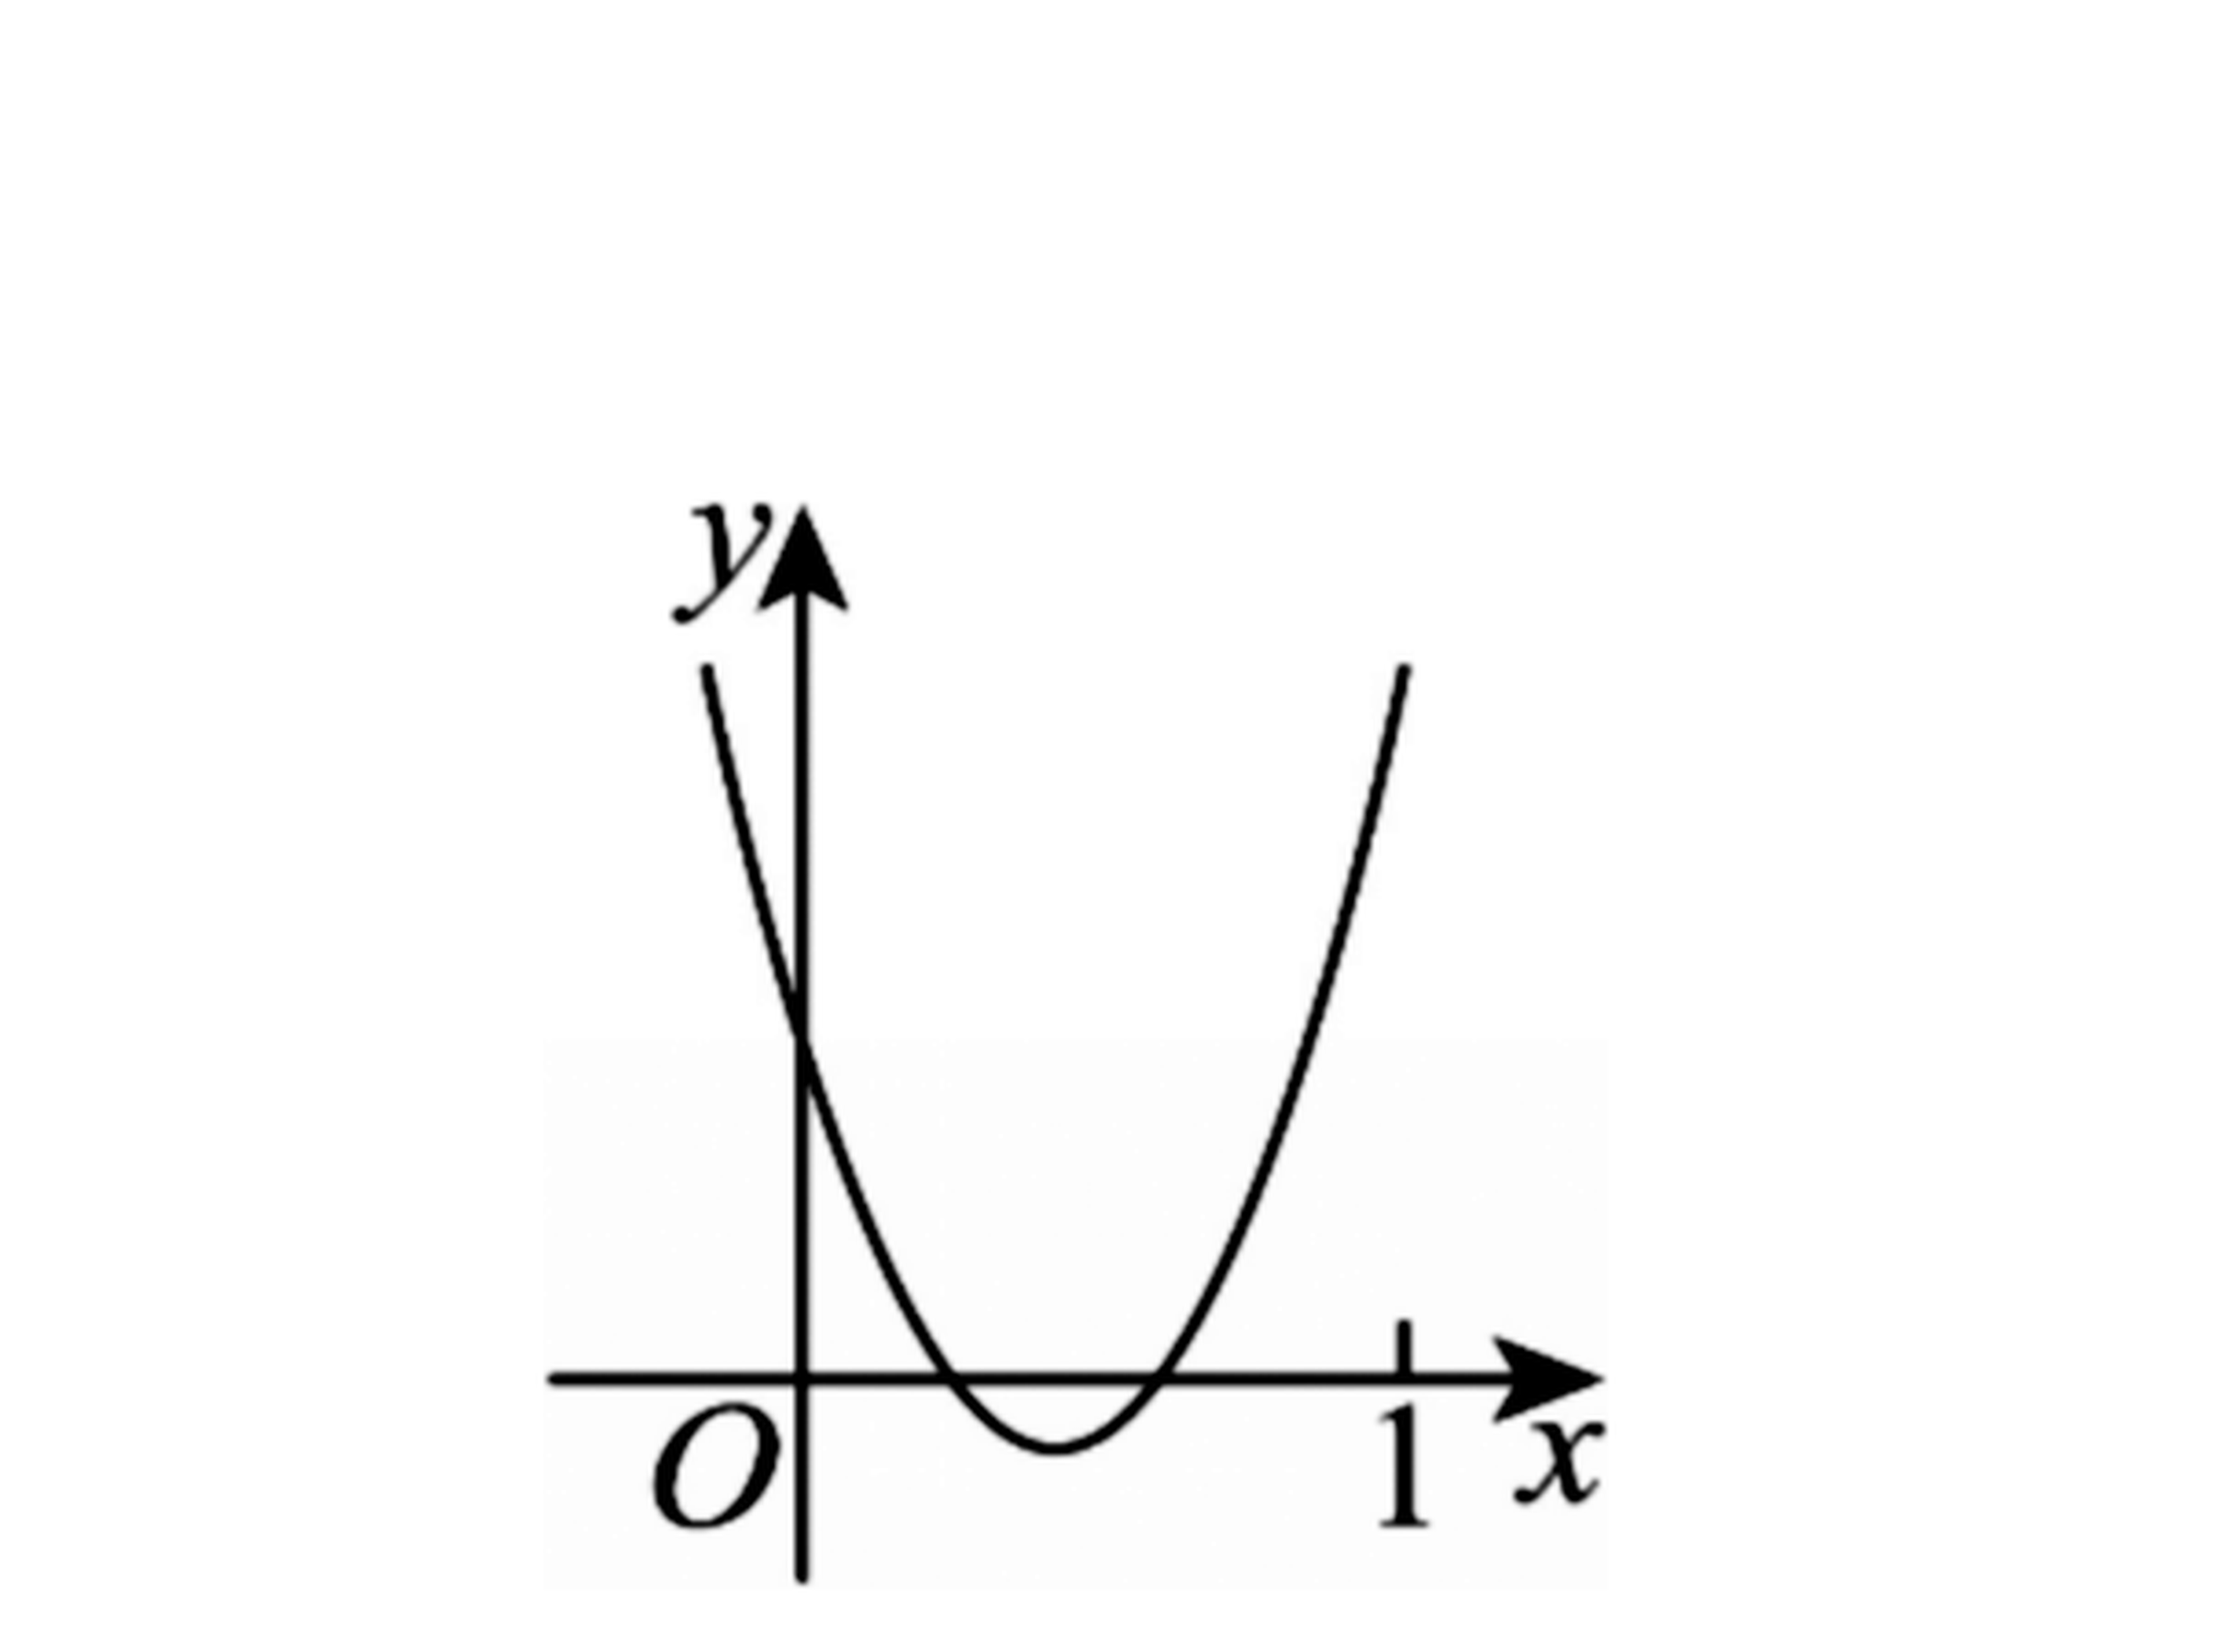
\includegraphics[width=0.32\textwidth]{figures/gao154_q15_stem.png}
\end{center}

\keepwithprev
\begin{center}
% 四幅指数函数图像选项取 05 页上半，按原卷 2×2 排布合并为一张，去粉色水印、去色、4× LANCZOS 放大；三版都出
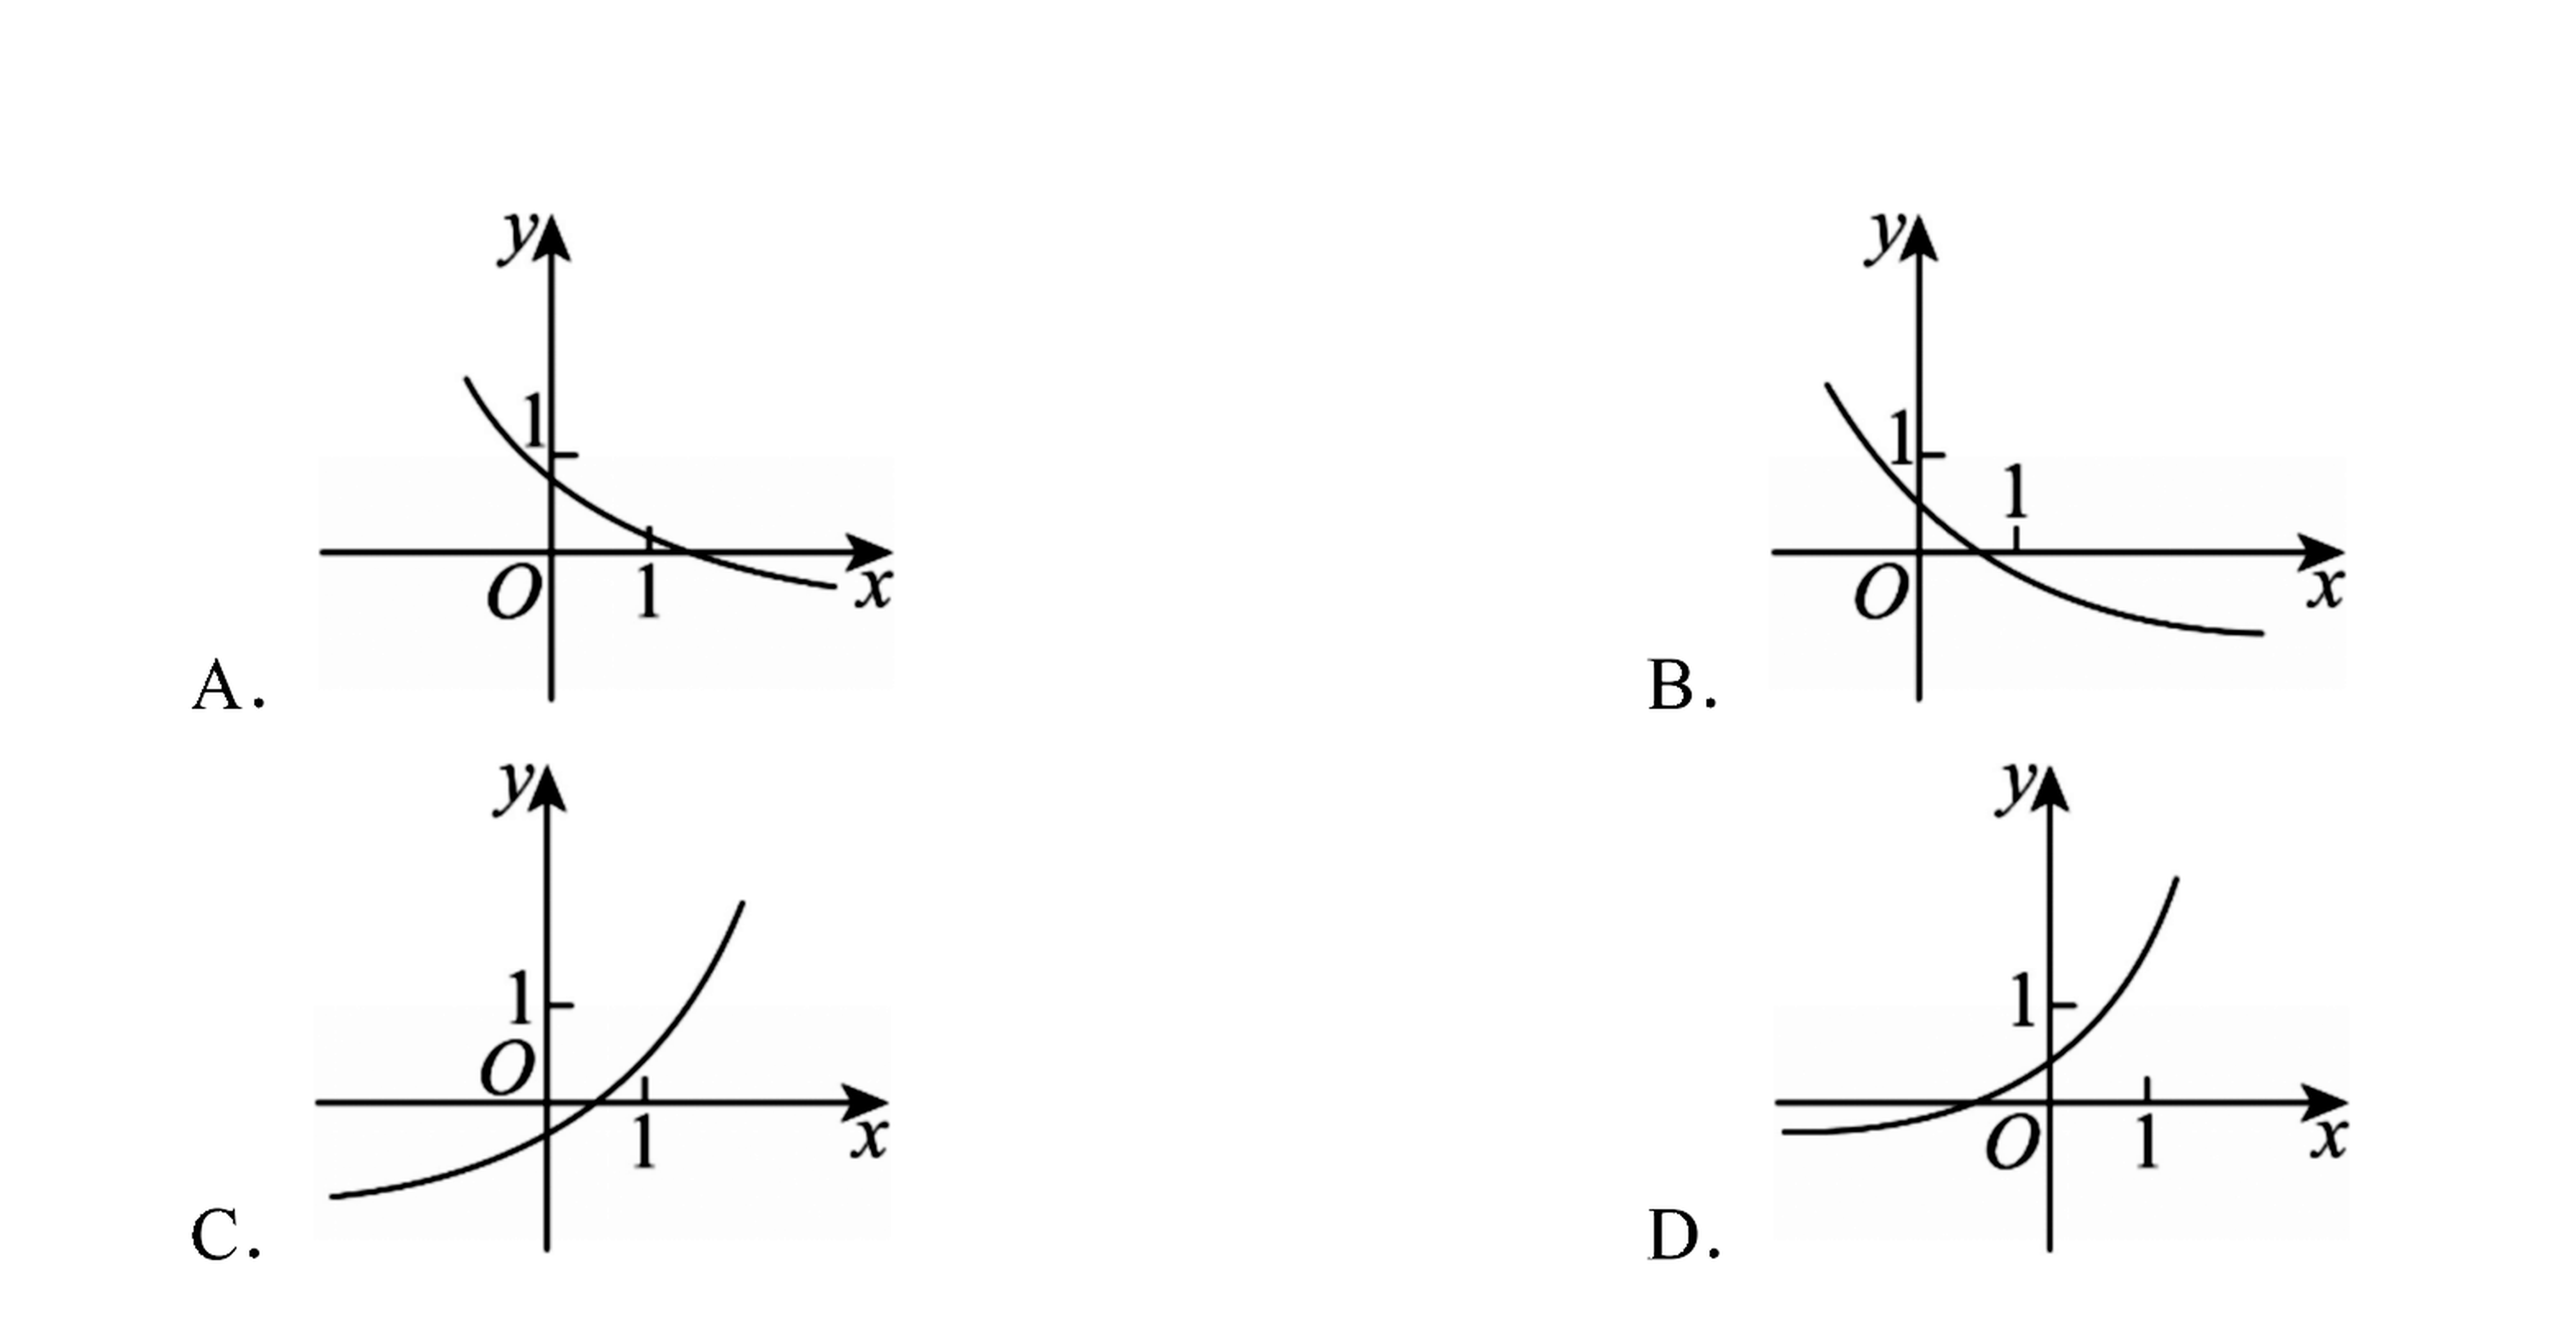
\includegraphics[width=0.80\textwidth]{figures/gao154_q15_opts.png}
\end{center}

\ifanswer
\solbegin
\step{由题意得 $0<a<b<1$，所以 $g(x)=a^x-b$ 在定义域 $\R$ 上严格减.}
\step{$g(0)=a^0-b=1-b>0$，$g(1)=a^1-b=a-b<0$，故 B 符合题意.}
\step{故选 $B$.}
\solend
\fi

% === Q16 === 高斯取整；解析 13 行，故选 C
\item 设 $[a]$ 表示不超过 $a$ 的最大整数，如 $[1.2]=1$，$[-3.2]=-4$，若 $x$、$y$、$z$ 为正实数，则 $\left[\dfrac{y+z}{x}\right]+\left[\dfrac{z+x}{y}\right]+\left[\dfrac{x+y}{z}\right]$ 的最小值为\mbox{（\quad）}

\keepwithprev
A. 2\qquad\qquad B. 3\qquad\qquad C. 4\qquad\qquad D. 6

\ifanswer
\solbegin
\step{若 $x$、$y$、$z$ 为正实数，}
\step{结合基本不等式得 $\dfrac{y+z}{x}+\dfrac{z+x}{y}+\dfrac{x+y}{z}=\dfrac yx+\dfrac xy+\dfrac zx+\dfrac xz+\dfrac zy+\dfrac yz$}
\step{$\geqslant2\sqrt{\dfrac yx\cdot\dfrac xy}+2\sqrt{\dfrac zx\cdot\dfrac xz}+2\sqrt{\dfrac zy\cdot\dfrac yz}=6$，当且仅当 $x=y=z$ 时取等号，}
\step{即 $\dfrac{y+z}{x}$，$\dfrac{z+x}{y}$，$\dfrac{x+y}{z}$ 中至少有一个不小于 2，不妨设 $\dfrac{y+z}{x}\geqslant\dfrac{z+x}{y}\geqslant\dfrac{x+y}{z}$，}
\step{$[a]$ 表示不超过 $a$ 的最大整数和 $\dfrac{y+z}{x}$，$\dfrac{z+x}{y}$，$\dfrac{x+y}{z}$ 中至少有一个不小于 2，}% 原卷此行把两句连写，照录未改（见 ⑤ 3）
\step{得 $\left[\dfrac{y+z}{x}\right]\geqslant2$，所以 $\left[\dfrac{y+z}{x}\right]+\left[\dfrac{z+x}{y}\right]+\left[\dfrac{x+y}{z}\right]\geqslant2$，}
\step{假设 $\left[\dfrac{y+z}{x}\right]+\left[\dfrac{z+x}{y}\right]+\left[\dfrac{x+y}{z}\right]$ 的最小值为 2，$\left[\dfrac{y+z}{x}\right]=2$，$\left[\dfrac{z+x}{y}\right]+\left[\dfrac{x+y}{z}\right]=0$，}
\step{所以 $2\leqslant\dfrac{y+z}{x}<3$，$0<\dfrac{z+x}{y}<1$，$0<\dfrac{x+y}{z}<1$，所以 $2<\dfrac{y+z}{x}+\dfrac{z+x}{y}+\dfrac{x+y}{z}<5$，}
\step{与 $\dfrac{y+z}{x}+\dfrac{z+x}{y}+\dfrac{x+y}{z}\geqslant6$ 矛盾，假设不成立，A 错误；}
\step{假设 $\left[\dfrac{y+z}{x}\right]+\left[\dfrac{z+x}{y}\right]+\left[\dfrac{x+y}{z}\right]$ 的最小值为 3，}
\step{则 $\left[\dfrac{y+z}{x}\right]=2$，$\left[\dfrac{z+x}{y}\right]=1$，$\left[\dfrac{x+y}{z}\right]=0$ 或 $\left[\dfrac{y+z}{x}\right]=3$，$\left[\dfrac{z+x}{y}\right]=\left[\dfrac{x+y}{z}\right]=0$，}
\step{同理可得 $3<\dfrac{y+z}{x}+\dfrac{z+x}{y}+\dfrac{x+y}{z}<6$，显然不成立，B 错误；}
\step{假设 $\left[\dfrac{y+z}{x}\right]+\left[\dfrac{z+x}{y}\right]+\left[\dfrac{x+y}{z}\right]$ 的最小值为 4，易得 $4<\dfrac{y+z}{x}+\dfrac{z+x}{y}+\dfrac{x+y}{z}<7$，}
\step{若取 $x=100$，$y=103$，$z=104$，则 $\left[\dfrac{y+z}{x}\right]=2$，$\left[\dfrac{z+x}{y}\right]=1$，$\left[\dfrac{x+y}{z}\right]=1$，}
\step{即 $\left[\dfrac{y+z}{x}\right]+\left[\dfrac{z+x}{y}\right]+\left[\dfrac{x+y}{z}\right]=4$，假设成立，C 正确，D 错误.}
\step{故选 $C$.}
\solend
\fi

\end{enumerate}

\bigsec{三、解答题}

\begin{enumerate}
\setcounter{enumi}{16}

% === Q17 === $B\subset A$ 单线照录；cases 块；解析 5 行
\item 设集合 $A=\{x\mid x^2+2x-3<0\}$，集合 $B=\{x\mid\lvert x+a\rvert<1\}$.

(1) 若 $a=3$，求 $A\cup B$；

(2) 设命题 $p:x\in A$，命题 $q:x\in B$，若 $p$ 是 $q$ 成立的必要不充分条件，求实数 $a$ 的取值范围.

\ifanswer
\solbegin
\step{(1) $A=(-3,1)$，}
\step{当 $a=3$ 时，$\lvert x+3\rvert<1$，解得 $-4<x<-2$，所以 $B=(-4,-2)$，}
\step{所以 $A\cup B=(-4,1)$.}
\step{(2) 因为 $p$ 是 $q$ 成立的必要不充分条件，所以 $B\subset A$.}
\step{因为 $A=(-3,1)$，$B=(-a-1,-a+1)$，所以 $\begin{cases}-a-1\geqslant-3\\-a+1<1\end{cases}$ 或 $\begin{cases}-a-1>-3\\-a+1\leqslant1\end{cases}$，解得 $0\leqslant a\leqslant2$.}
\solend
\fi

% === Q18 === 判别式 \Delta 两处照录；解析 9 行
\item 已知关于 $x$ 的一元二次方程 $x^2-mx+4m^2-3=0$ 的两个实根分别为 $x_1,x_2$.

(1) 若 $x_1,x_2$ 满足 $x_1+x_2=x_1x_2$，求实数 $m$ 的值；

(2) 求 $x_1^2+x_2^2$ 的最小值.

\ifanswer
\solbegin
\step{(1) 由韦达定理 $x_1+x_2=m$，$x_1x_2=4m^2-3$，}
\step{$\Delta=m^2-4(4m^2-3)=-15m^2+12\geqslant0$，即 $m^2\leqslant\dfrac45$.}
\step{由 $x_1+x_2=x_1x_2$ 得 $m=4m^2-3$，即 $4m^2-m-3=0$，}
\step{解得 $m=1$ 或 $m=-\dfrac34$.}
\step{$m=1$ 时 $m^2=1>\dfrac45$，$\Delta<0$，舍去；}
\step{$m=-\dfrac34$ 时 $m^2=\dfrac9{16}<\dfrac45$，符合，故 $m=-\dfrac34$.}
\step{(2) $x_1^2+x_2^2=(x_1+x_2)^2-2x_1x_2=m^2-2(4m^2-3)=-7m^2+6$，}
\step{函数 $y=-7m^2+6$ 开口向下，对称轴为 $m=0$，}% 原卷此处称求「最小值」，实为闭区间 $m^2\le\frac45$ 上的最小值，照录未改（见 ⑤ 4）
\step{故 $y_{\min}=-7\cdot\dfrac45+6=-\dfrac{28}{5}+\dfrac{30}{5}=\dfrac25$.}
\solend
\fi

% === Q19 === 全称命题；cases 块；解析 9 行
\item 设命题 $p$：对任意 $x\in\R$，不等式 $2mx^2+2mx+1>0$ 恒成立，$q:m\in\{m\mid\log_2(m-1)<1\}$.

(1) 若 $p$ 为真命题，求实数 $m$ 的取值范围；

(2) 若命题 $p$、$q$ 有且只有一个是真命题，求实数 $m$ 的取值范围.

\ifanswer
\solbegin
\step{(1) 由 $p$ 为真命题，得 $\forall x\in\R$，不等式 $2mx^2+2mx+1>0$ 恒成立，}
\step{当 $m=0$ 时，$1>0$ 恒成立；}
\step{当 $m\ne0$ 时，$\begin{cases}2m>0\\\Delta=4m^2-8m<0\end{cases}$，解得 $0<m<2$；}
\step{综上，$0\leqslant m<2$，即 $m$ 的取值范围是 $[0,2)$；}
\step{(2) 若 $q$ 为真，则有 $\log_2(m-1)<1$，得 $0<m-1<2$，解得 $1<m<3$，}
\step{因此命题 $q:m\in\{m\mid1<m<3\}$，由 (1) 得命题 $p:\{m\mid0\leqslant m<2\}$，}
\step{而命题 $p$、$q$ 有且只有一个是真命题，}
\step{当 $p$ 真 $q$ 假时，$\begin{cases}0\leqslant m<2\\m\leqslant1\text{ 或 }m\geqslant3\end{cases}$，解得 $0\leqslant m\leqslant1$，}
\step{当 $p$ 假 $q$ 真时，$\begin{cases}m<0\text{ 或 }m\geqslant2\\1<m<3\end{cases}$，解得 $2\leqslant m<3$，}
\step{故实数 $m$ 的取值范围是 $\{m\mid0\leqslant m\leqslant1\text{ 或 }2\leqslant m<3\}$.}
\solend
\fi

% === Q20 === Labubu 成本题；解析 10 行
\item Labubu 公司拟在 2027 年初推出智能机器人系列玩偶（单位：套）. 根据以往经验，其中一条生产线每月生产 $x$ 套玩具的成本 $P$ 由两部分费用（单位：元）构成：

(i) 固定成本（与生产玩具套数 $x$ 无关），总计 160000 元；

(ii) 每生产 $x$ 套需另投入的生产成本 $c(x)$ 元，其中 $c(x)=10x+\dfrac1{100}x^2$.

(1) 假设该生产线每月生产出的玩具能全部售出，问：该生产线每月生产玩具多少套时，可使得平均每套所需成本费用最少？此时每套玩具的成本费用是多少？

(2) 假设该生产线每月生产出的玩具能全部售出，但随着 $x$ 的增大，每月生产所需的直接总成本在急剧增加，因此售价也需随着 $x$ 的增大而适当增加. 设每套玩具的售价为 $q(x)$ 元，$q(x)=a+\dfrac xb$（$a,b\in\R$）. 若当月产量为 10000 套时利润最大，此时每套售价为 150 元，试求 $a,b$ 的值.（利润=销售收入$-$成本费用）

\ifanswer
\solbegin
\step{(1) 每月总成本 $P=160000+10x+\dfrac1{100}x^2$，}
\step{平均每套成本为 $\dfrac Px=\dfrac{160000}{x}+10+\dfrac x{100}\geqslant10+2\sqrt{\dfrac{160000}{x}\cdot\dfrac x{100}}=90$.}
\step{等号成立当且仅当 $\dfrac{160000}{x}=\dfrac x{100}$ 时，即 $x=4000$ 时取等号，}
\step{所以每月生产 4000 套时平均每套成本最少，此时每套成本为 90 元.}
\step{(2) 利润 $W(x)=x\cdot q(x)-P=\left(\dfrac1b-\dfrac1{100}\right)x^2+(a-10)x-160000$.}
\step{要在 $x=10000$ 处取得最大值，需 $\dfrac1b-\dfrac1{100}<0$，且对称轴为 $x=10000$，}
\step{故 $-\dfrac{a-10}{2\left(\frac1b-\frac1{100}\right)}=10000$，即 $a-10=-20000\left(\dfrac1b-\dfrac1{100}\right)$.}
\step{又 $q(10000)=a+\dfrac{10000}{b}=150$.}
\step{令 $t=\dfrac1b$，则 $a=150-10000t$，}
\step{代入上式 $140-10000t=-20000t+200$，解得 $t=\dfrac3{500}$，即 $b=\dfrac{500}{3}$；}
\step{再由 $a=150-10000\times\dfrac3{500}=150-60=90$，所以 $a=90$，$b=\dfrac{500}{3}$.}
\solend
\fi

% === Q21 === $A^+$／$A^-$ 新定义；$A\subseteq$ 带下划线照录、\varnothing；解析 16 行
\item 设集合 $A$ 为非空数集，定义 $A^+=\{x\mid x=a+b,a,b\in A\}$，$A^-=\{x\mid x=\lvert a-b\rvert,a,b\in A\}$.

(1) 若集合 $A=\{-1,1\}$，写出集合 $A^+$ 及 $A^-$；

(2) 若集合 $A=\{x_1,x_2,x_3,x_4\}$，$x_1<x_2<x_3<x_4$，且 $A^-=A$，求证：$x_1+x_4=x_2+x_3$；

(3) 若集合 $A\subseteq\{x\mid0\leqslant x\leqslant2020,x\in\N\}$，且 $A^+\cap A^-=\varnothing$，求集合 $A$ 元素的个数的最大值.

\ifanswer
\solbegin
\step{(1) 由 $A=\{-1,1\}$，得 $A^+=\{-2,0,2\}$，$A^-=\{0,2\}$；}
\step{(2) 由于集合 $A=\{x_1,x_2,x_3,x_4\}$，$x_1<x_2<x_3<x_4$，且 $A^-=A$，}
\step{所以 $A^-$ 中也只包含四个元素，即 $A^-=\{0,x_2-x_1,x_3-x_1,x_4-x_1\}$，}
\step{剩下的 $x_3-x_2=x_4-x_3=x_2-x_1$，所以 $x_1+x_4=x_2+x_3$；}
\step{(3) 设 $A=\{a_1,a_2,\cdots,a_k\}$ 满足题意，其中 $a_1<a_2<\cdots<a_k$，}
\step{则 $2a_1<a_1+a_2<a_1+a_3<\cdots<a_1+a_k<a_2+a_k<a_3+a_k<\cdots<a_{k-1}+a_k<2a_k$，所以 $\lvert A^+\rvert\geqslant2k-1$，}
\step{且 $a_1-a_1<a_2-a_1<a_3-a_1<\cdots<a_k-a_1$，所以 $\lvert A^-\rvert\geqslant k$，}
\step{因为 $A^+\cap A^-=\varnothing$，所以 $\lvert A^+\cup A^-\rvert=\lvert A^+\rvert+\lvert A^-\rvert\geqslant3k-1$，}
\step{$A^+\cup A^-$ 中最小的元素为 0，最大的元素为 $2a_k$，所以 $\lvert A^+\cup A^-\rvert\leqslant2a_k+1$，}
\step{所以 $3k-1\leqslant2a_k+1\leqslant4041$（$k\in\N^*$），所以 $k\leqslant1347$，}
\step{实际上当 $A=\{674,675,676,\cdots,2020\}$ 时满足题意，证明如下：}
\step{设 $A=\{m,m+1,m+2,\cdots,2020\}$，$m\in\N$，}
\step{则 $A^+=\{2m,2m+1,2m+2,\cdots,4040\}$，$A^-=\{0,1,2,\cdots,2020-m\}$，}
\step{由题意得 $2020-m<2m$，即 $m>673\dfrac13$，}
\step{故 $m$ 的最小值为 674，于是当 $m=674$ 时，$A$ 中元素最多，}
\step{即 $A=\{674,675,676,\cdots,2020\}$ 时满足题意，}
\step{综上所述，集合 $A$ 中元素的个数的最大值是 1347.}
\solend
\fi

\end{enumerate}

\bigsec{附加题}

\begin{enumerate}

% === 附加题 1 === 另起编号 1；「n 元集和集」弯引号；解析 6 行
\item 设集合 $A=\{a_1,a_2,a_3,a_4\}$，$C=\{2,3,4,6\}$，新定义：集合 $A$ 中所有含 $n$ 个元素的子集中 $n$ 个元素之和的不同值组成的集合为“$n$ 元集和集”. 若 $A$ 的“3 元集和集”为 $C$，则集合 $A=$\blankline[4.4em].

\ifanswer
\solbegin
\step{集合 $A$ 的 3 元子集共有 4 个：$\{a_1,a_2,a_3\}$，$\{a_1,a_2,a_4\}$，$\{a_1,a_3,a_4\}$，$\{a_2,a_3,a_4\}$，}
\step{集合 $C=\{a_1+a_2+a_3,a_1+a_2+a_4,a_1+a_3+a_4,a_2+a_3+a_4\}$，}
\step{不妨令 $a_1<a_2<a_3<a_4$，}
\step{则 $a_1+a_2+a_3<a_1+a_2+a_4<a_1+a_3+a_4<a_2+a_3+a_4$，}
\step{而 $C=\{2,3,4,6\}$，因此 $\begin{cases}a_1+a_2+a_3=2\\a_1+a_2+a_4=3\\a_1+a_3+a_4=4\\a_2+a_3+a_4=6\end{cases}$，相加化简得 $a_1+a_2+a_3+a_4=5$，}
\step{解得 $a_1=-1$，$a_2=1$，$a_3=2$，$a_4=3$，所以 $A=\{-1,1,2,3\}$.}
\solend
\fi

% === 附加题 2 === 解析配图（仅答案版出）；四选项；解析 15 行，故选 A
\item 已知函数 $f(x)=\log_p x+q$，其中 $p>0$ 且 $p\ne1$，曲线 $y=f(x)$ 经过 $P(1,2)$、$Q(2,3)$ 两点. 设 $g(x)=f(x)\cdot[f(x)-2]$，若 $\lvert g(a)\rvert=\lvert g(b)\rvert=\lvert g(c)\rvert=\lvert g(d)\rvert$，且 $a<b<c<d$，则 $ad(b+c)$ 的取值范围为\mbox{（\quad）}

\keepwithprev
A. $\left(\dfrac14,\dfrac5{16}\right)$\qquad B. $\left(\dfrac18,\dfrac5{16}\right)$\qquad C. $\left(\dfrac14,\dfrac25\right)$\qquad D. $\left(\dfrac18,\dfrac25\right)$

\ifanswer
\solbegin
\step{函数 $f(x)=\log_p x+q$，且曲线 $y=f(x)$ 经过点 $P(1,2)$ 和 $Q(2,3)$，}
\step{所以 $\begin{cases}f(1)=q=2\\f(2)=\log_p2+q=3\end{cases}$，解得 $p=2$，$q=2$，$f(x)=\log_2 x+2$.}
\step{不妨设 $\lvert g(x)\rvert=k$，令 $\log_2 x=m$，则 $f(x)\cdot[f(x)-2]=m(m+2)=m^2+2m$，}
\step{画出函数 $y=\lvert m^2+2m\rvert$ 的图象，如图所示，}
\begin{center}
% $y=|m(m+2)|$ 图像取 11 页右上，去粉色水印、去色、4× LANCZOS 放大；仅答案版出
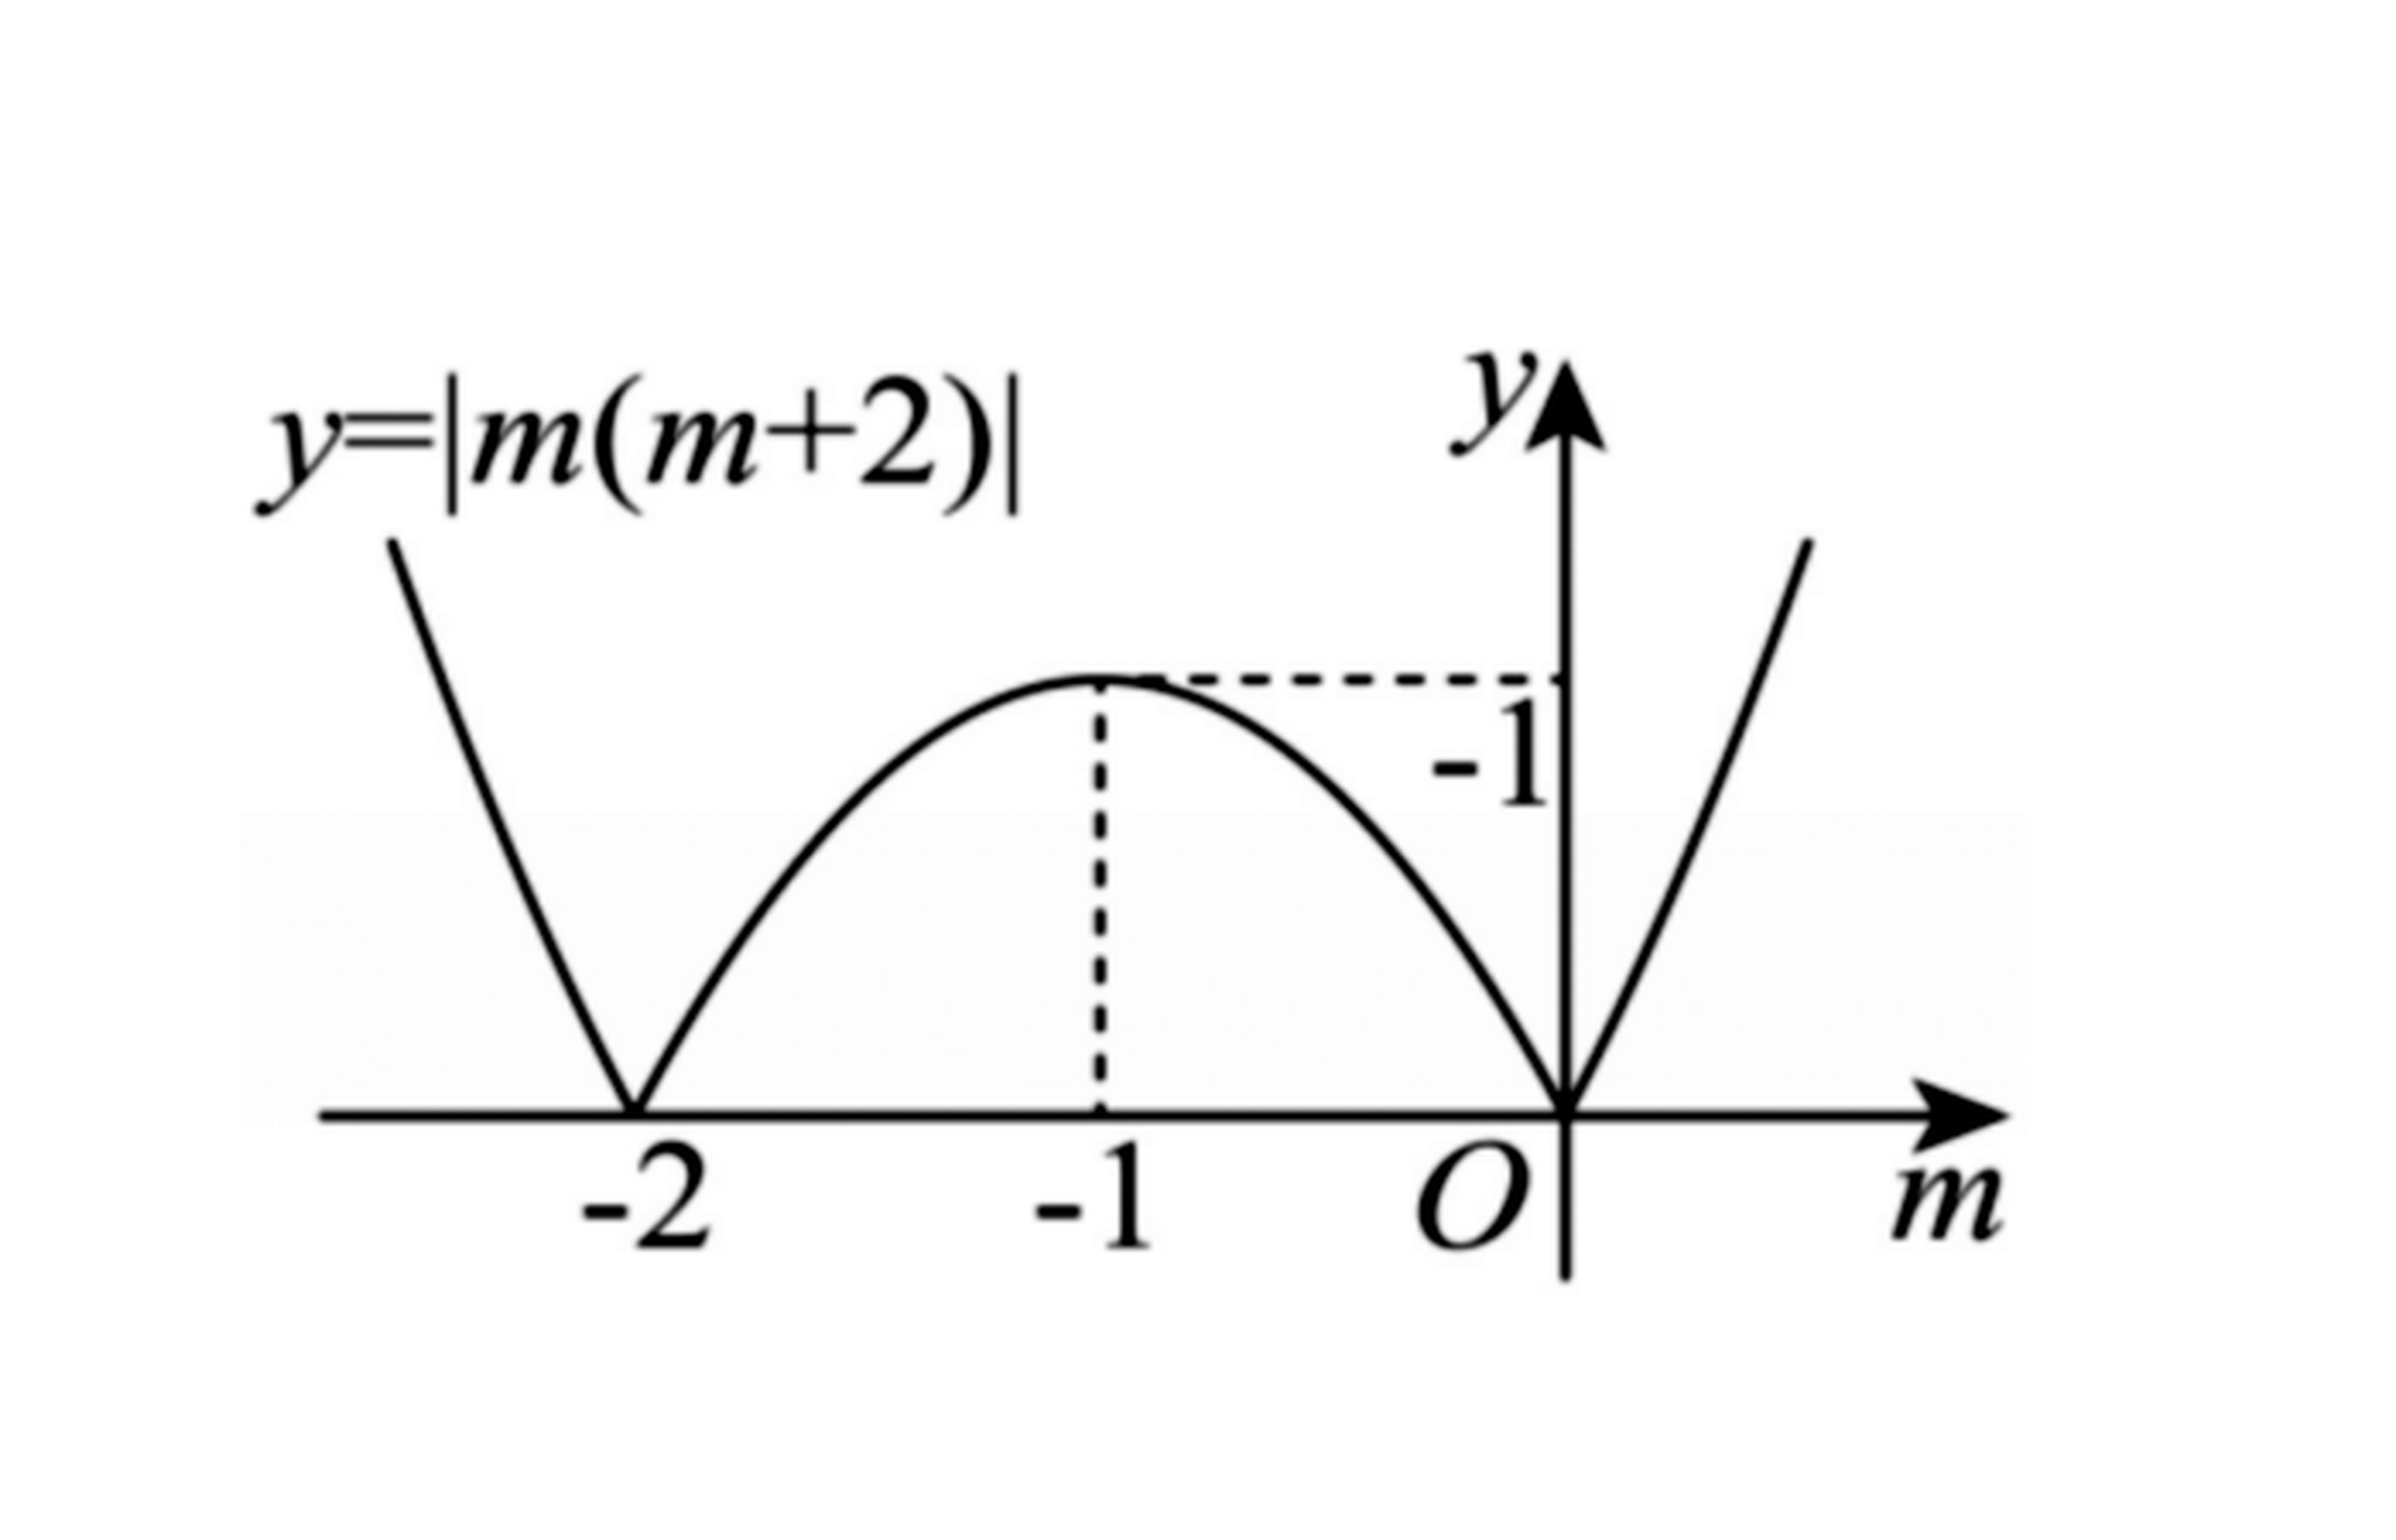
\includegraphics[width=0.46\textwidth]{figures/gao154_fujia2.png}
\end{center}
\step{由图像得 $k\in(0,1)$，}
\step{所以方程 $m^2+2m=k$ 和 $m^2+2m=-k$ 各有两个不同的根，}
\step{其中方程 $m^2+2m-k=0$ 的两根为 $m=-1\pm\sqrt{1+k}$，}
\step{方程 $m^2+2m+k=0$ 的两根为 $m=-1\pm\sqrt{1-k}$，}
\step{所以 $m_1=-1-\sqrt{1+k}$，$m_2=-1-\sqrt{1-k}$，$m_3=-1+\sqrt{1-k}$，$m_4=-1+\sqrt{1+k}$，且 $m_1<m_2<m_3<m_4$，}
\step{由 $m=\log_2 x$，则 $x=2^m$，}
\step{所以 $a=2^{-1-\sqrt{1+k}}$，$b=2^{-1-\sqrt{1-k}}$，$c=2^{-1+\sqrt{1-k}}$，$d=2^{-1+\sqrt{1+k}}$，}
\step{所以 $ad=2^{-1-\sqrt{1+k}}\times2^{-1+\sqrt{1+k}}=2^{(-1-\sqrt{1+k})+(-1+\sqrt{1+k})}=2^{-2}=\dfrac14$，}
\step{$b+c=2^{-1-\sqrt{1-k}}+2^{-1+\sqrt{1-k}}=\dfrac{2^{-\sqrt{1-k}}+2^{\sqrt{1-k}}}{2}$，}
\step{令 $s=\sqrt{1-k}$，其中 $s\in(0,1)$，则 $b+c=\dfrac12\left(2^{-s}+2^s\right)$，}
\step{设函数 $y=2^s+\dfrac1{2^s}$，令 $r=2^s\in(1,2)$，所以 $y=r+\dfrac1r$ 在 $(1,2)$ 上严格增，}
\step{所以函数 $y=2^s+\dfrac1{2^s}$ 在 $(0,1)$ 上严格增，所以 $y=2^s+\dfrac1{2^s}\in\left(2,\dfrac52\right)$，}
\step{所以 $b+c=\dfrac{2^{-s}+2^s}{2}\in\left(1,\dfrac54\right)$，$ad(b+c)=\dfrac{b+c}{4}\in\left(\dfrac14,\dfrac5{16}\right)$，}
\step{所以 $ad(b+c)$ 的取值范围是 $\left(\dfrac14,\dfrac5{16}\right)$，故选 $A$.}
\solend
\fi

\end{enumerate}

\end{document}
"
%
% ① 原始材料：微信公众号"魔都数学加油站"文章，连载"27学年高一154"，原文标题
% "27学年高一154——2026-2027年上海市徐汇中学高一上期中"；
% 原文链接：https://mp.weixin.qq.com/s/Qs2T7Zwsug-KKFE2wefDUg 。
% 正文为 12 张 PNG 页（01/03/04/05/07/11/12 为 2560×3620，
% 02/06/08/09/10 为 4762×6735，同一篇各页分辨率混排，逐页按各自分辨率裁图核对）。
% 体例：讲评版——一、填空题 3—12（10 题）、二、选择题 13—16（4 题）、
% 三、解答题 17—21（5 题）、附加题 1—2（2 题，原卷**另起编号**"1." "2."，
% 不与正题连号，同 高一a 成例），共 21 题；全卷每题均印【解析】
% （逐题核实，见 ② ②）。题目、答案、解析均据原图转录；卷面粉红色水印
% "魔都数学加油站"及公众号页脚未录入。
% 全卷插图清单（逐页通读 12 页确认）：3 组——
%   · Q15 题干配图（$f(x)=(x-a)(x-b)$ 抛物线，04 页右下：x/y 轴、O、1、
%     开口向上两零点均在 (0,1) 内），三版都出，裁 figures/gao154_q15_stem.png；
%   · Q15 四幅图像选项（05 页上半 2×2 排布，A/B/C/D 四幅指数函数图像，
%     合并成一张，照 高一136 Q13/Q22 成例），三版都出，
%     裁 figures/gao154_q15_opts.png；
%   · 附加题第 2 题解析配图（$y=\lvert m(m+2)\rvert$ 图像，11 页右上：
%     W 形折线、$-2$、$-1$、O、虚线 $y=1$ 与 $m=-1$），仅答案版出，
%     裁 figures/gao154_fujia2.png；
%   3 图均取自原卷截图，去粉色水印、去色、4× LANCZOS 放大；Q15 题干图
%   左侧题干残字"的图"已裁白。其余各页逐页确认无其它题目配图、无表格；
%   12 页下半仅水印、无正文。
%
% 卷首标题：原卷印作"2026-2027 年徐汇中学高一上期中"，年份区间按全稿惯例排 en dash；
% 原卷卷面未印副标题，本稿按同期中卷知识模块口径补出"集合与常用逻辑用语、不等式、函数"。
%
% ② 与原卷的排版差异：
%   ① 原文从第 3 题起，本稿保留原题号；共 21 题四节，正题到 21，附加题另起编号
%      1—2（\bigsec{附加题} 后 \begin{enumerate} 不 \setcounter，同 高一a 成例）；
%   ② 全 21 题均印【解析】、用 \solbegin…\solend，无只印【答案】或答案印括号内的题；
%      四道正题选择题答案在解析末句"故选 C／A／B／C"（Q13—Q16）、附加题第 2 题
%      答案在解析末句"故选 A"，括号 \mbox{（\quad）} 留空、不另提 \ans{}；
%      答案版【答案】/【解析】标记数 = 21 = 全卷题数；
%   ③ 原卷卷面未印副标题，本稿按知识模块口径补出；
%   ④ 原卷填空横线按全稿惯例排 \blankline[4.4em]；选择题括号排 \mbox{（\quad）}、
%      四道正题选择题与附加题第 2 题的选项段前按惯例各加 \keepwithprev
%      （Q15 与附加题 2 的选项段是整块图，\keepwithprev 后接 \begin{center}）；
%      解答题不留作答区、不加 \anspace（原卷为讲评版）；
%   ⑤ 数集黑板粗体：Q4"$x,y\in R$"、Q9"$x\in\R$"、Q13 无、
%      Q15"定义域 $\R$"、Q19"$\forall x\in\R$"、Q21"$x\in\N$"与"$k\in\N^*$"、
%      Q20"$a,b\in\R$"、附加题 2 无——原卷印斜体或正体粗体 R/N/N*，
%      按全稿惯例归一 \R／\N／\N^*；绝对值排 \lvert…\rvert
%      （Q5、Q9、Q12、Q13、Q16、Q21、附加题 2），集合描述竖线排 \mid
%      （Q5、Q17、Q19、Q21），不等号按全稿惯例排 \leqslant／\geqslant；
%      空集 \varnothing（Q21 题干 (3)）；
%   ⑥ 子集符号逐处照录、不得统一：Q6 题干印"$\{1,2\}\subset M\subseteq\{1,2,3,4,5\}$"
%      （前单线 ⊂、后带下划线 ⊆，同句两形并用），解析亦两形并用；
%      Q17 解析 (2)"$B\subset A$"印单线 ⊂；Q21 题干 (3)"$A\subseteq\{x\mid\cdots\}$"
%      印带下划线 ⊆——逐处放大核，分别 \subset／\subseteq，照录未统一（见 ④）；
%   ⑦ 判别式 Δ/△：Q18 解析 (1)"$\Delta=m^2-4(4m^2-3)$"与 Q19 解析 (1)
%      "$\Delta=4m^2-8m<0$"两处均印等腰偏高粗三角、照录 \Delta；本卷无扁等边
%      细线 \triangle 用例（见 ④）；
%   ⑧ 中文弯引号照录：Q4"设 $x$、$y\in\R$. 若 $x+y>2$，则 $x>1$ 或 $y>1$"、
%      附加题 1"$n$ 元集和集"与"3 元集和集"；注释里一律 ASCII 引号；
%      数学式内 CJK 用 \text{}（Q5 解集描述"或"、Q19 集合描述的"或"）；
%   ⑨ "图像／图象"逐处放大核：Q15 题干与解析印"图象"（象，无亻）、
%      Q16 无、附加题 2 解析印"图象"与"图像"（"画出函数…的图象"、
%      "由图像得"——两形并用，逐处照录未统一）；Q13/Q14 无数集图像字样；
%      半角逗号在数学组之间是全稿惯例、非笔误，逐处照录（Q3、Q10、Q16、
%      Q18、Q20、Q21 的 $x_1,x_2$ 之类）；行末西文句点 ASCII `.`；
%      行中全角逗号／顿号照录（Q6"3，4，5"、Q20"（单位：元）"、
%      附加题 1"$a_1,a_2,a_3,a_4$"）；
%   ⑩ 复杂式照录别简化：Q3 $a^{\frac{12}{7}}\cdot\left(\frac17\right)^{\frac17}
%      \cdot\sqrt[7]{a^4}$ 与 $7^{-\frac17}a^{\frac{16}{7}}$、Q7 $x^{-m}$、
%      Q8 $\frac{b-2a+2}{2a}$、Q11 $\frac{9+4\sqrt2}{6}$、Q12 $506\frac29$ 与
%      $506\frac49$、Q16 高斯取整 $[a]$、Q20 $c(x)=10x+\frac1{100}x^2$ 与
%      $q(x)=a+\frac xb$、Q21 $A^+$／$A^-$ 与 $|A^+|\geqslant2k-1$、
%      附加题 2 $m=-1\pm\sqrt{1+k}$ 与 $ad(b+c)$；
%      \left…\right 不得拆到不同 $…$ 组（Q5 $\left\{x\mid\cdots\right\}$、
%      Q20 $\left(\frac1b-\frac1{100}\right)$、附加题 2 $\left(\frac14,\frac5{16}\right)$）；
%      cases 块一律 \begin{cases}…\end{cases}；
%   ⑪ 一条 \step = 原卷解析的一个印刷行，cases 块整体算一个印刷行；别并折行、
%      别拆行。Q11 九行、Q12 六行、Q16 十六行、Q20 十一行、Q21 十七行、
%      附加题 2 十八行均按印刷行逐条断，不丢行；
%   ⑫ 配图：Q15 题干小图（三版都出）放 \item 内题干之后 \begin{center}，
%      Q15 四幅选项图（三版都出）放 \keepwithprev 之后的 \begin{center}，
%      Q15 用 \needvspace 守卫把"题干＋两图"整块推走（守卫放 \item 之前，
%      见 高一145 Q14/Q20 与 高一136 Q13 成例）；附加题 2 解析配图（仅答案版出）
%      放 \ifanswer 内 \solbegin…\solend 的 \step 之间（高一73 第 16 题成例）；
%   ⑬ 原卷解析内无红色"法一／法二"之类小标题，故本卷无 \stepm；红色水印
%      "魔都数学加油站"不录入；
%   ⑭ 跨页续印按题合并：见 ⑥；
%
% ③ 行数复核：一条 \step = 原卷解析的一个印刷行，cases 块作一个印刷行计。
%   逐题数（主会话逐页核对定稿）：Q3：1；Q4：1；Q5：3；Q6：4；Q7：3；
%   Q8：1；Q9：5；Q10：4；Q11：9；Q12：6；Q13：5；Q14：4；Q15：3；
%   Q16：16；Q17：5；Q18：9；Q19：10；Q20：11；Q21：17；
%   附加题 1：6；附加题 2：18。
%   合计 141 条 \step（本卷无 \stepm），与原卷逐题印刷行相等。全卷 21 题
%   均设 \solbegin…\solend，答案版【答案】/【解析】标记数 = 21 = 全卷题数。
%
% ④ 判别式／子集符号结论（逐处放大原图照录、不得统一，主会话像素级复核）：
%   判别式：Q18 解析 (1)"$\Delta=m^2-4(4m^2-3)=-15m^2+12\geqslant0$"、
%      Q19 解析 (1)"$\Delta=4m^2-8m<0$"共 2 处，逐处放大确认印等腰偏高
%      粗三角（高>宽、右斜边粗），照录 \Delta；本卷无扁等边细线 \triangle
%      用例，无几何三角形符号。
%   子集：Q6 题干"$\{1,2\}\subset M\subseteq\{1,2,3,4,5\}$"前 ⊂ 单线、
%      后 ⊆ 带下划线（/tmp/gao154/z/zoom/q6_subset.png），解析两处同样两形
%      并用，分别照录 \subset／\subseteq；Q17 解析 (2)"$B\subset A$"单线
%      照录 \subset；Q21 题干 (3)"$A\subseteq\{x\mid\cdots\}$"带下划线
%      照录 \subseteq。本卷 ⊂ 与 ⊆ 混用逐处照录、不得统一。
%      空集 \varnothing（Q21 题干 (3)）、数集 \R／\N／\N^* 归一见 ② ⑤。
%
% ⑤ 存疑照录（放大原图确认，照录未改、正文对应处另有 % 注）：
%   1. Q7 题干印 $f(x)=(3m-1)x^{-m}$，解析首句却写"幂函数 $f(x)=x^\alpha$
%      的系数必须为 1"（用 $\alpha$ 作指数记号），随后 $f(2)=2^\alpha=8$
%      得 $\alpha=3$、$f(x)=x^3$——题干指数 $-m$ 与解析 $\alpha$ 记法不同，
%      系原卷记号前后不一，逐处照录未统一（放大 01/02 页确认）。
%   2. Q11 解析"因为 $u>0,v>0$，由基本不等式得 $\frac{4v}{u}+\frac{2u}{v}
%      \geqslant2\sqrt{\frac{4v}{u}\cdot\frac{2u}{v}}=4\sqrt2$"与
%      "所以 $\frac4u+\frac1v=\frac16\left(\frac4u+\frac1v\right)(2u+v)$"
%      照录，未把 $u,v$ 化简回 $x,y$。
%   3. Q16 解析把"$[a]$ 表示不超过 $a$ 的最大整数"与"和至少有一个不小于 2"
%      连写在同一行（原卷如此），照录未改；末行"假设成立，C 正确，D 错误"照录。
%   4. Q18 解析 (2)"函数 $y=-7m^2+6$ 开口向下，对称轴为 $m=0$"却称求
%      "$y_{\min}$"（实为在 $m^2\leqslant\frac45$ 闭区间上的最小值），
%      照录未改。
%   5. Q20 题干"$q(x)=a+\frac xb$（$a,b\in\R$）"与解析
%      "$W(x)=\left(\frac1b-\frac1{100}\right)x^2+(a-10)x-160000$"照录；
%      末行解得 $a=90,b=\frac{500}{3}$ 照录未化简。
%   6. Q21 题干 (3)"$A\subseteq\{x\mid0\leqslant x\leqslant2020,x\in\N\}$"
%      与解析"$3k-1\leqslant2a_k+1\leqslant4041$（$k\in\N^*$）"照录；
%      末行"集合 $A$ 中元素的个数的最大值是 1347"照录。
%   7. 附加题 1 解析"相加化简得 $a_1+a_2+a_3+a_4=5$"照录；
%      附加题 2 解析"由图像得 $k\in(0,1)$"与"由图像得"／"的图象"两形
%      并用逐处照录（见 ② ⑨）；末行"$ad(b+c)$ 的取值范围是
%      $\left(\frac14,\frac5{16}\right)$，故选 A"照录。
%   全卷除此 7 类外未发现其它笔误／自相矛盾处；21 题均印【解析】、
%   无只印【答案】或答案印括号内的题（见 ② ②）。
%
% ⑥ 跨页续印按题合并说明（逐页核实定稿）：Q3—Q5 题干＋解析在 01 页
%   （Q5 解析末 2 行续 01 页下半）；Q6、Q7 题干＋解析在 01 页下半
%   （Q7 解析余 2 行续 02 页顶）；Q8、Q9 题干＋解析在 02 页上半
%   （Q9 解析余 3 行续 02 页下半）；Q10 题干＋解析在 02 页下半；
%   Q11 题干＋解析前 6 行在 03 页上半、余 3 行续 03 页下半；
%   Q12 题干＋解析前 5 行在 03 页下半、末行续 04 页顶；"二、选择题"
%   标题与 Q13 题干＋选项＋解析在 04 页上半；Q14 题干＋选项＋解析、
%   Q15 题干＋题干配图在 04 页下半；Q15 四幅选项图＋解析、
%   Q16 题干＋选项＋解析首行在 05 页上半，Q16 解析余 12 行在
%   05 页下半—06 页上半；"三、解答题"标题与 Q17 题干＋两问＋解析
%   在 06 页下半；Q18 题干＋两问＋解析在 07 页上半—下半；
%   Q19 题干＋两问＋解析首行在 07 页下半，解析余 8 行在 08 页上半；
%   Q20 题干在 08 页下半，解析 (1) 4 行＋(2) 首 4 行在 08 页下半—09 页上半，
%   (2) 余 2 行在 09 页下半；Q21 题干＋三问＋解析 (1)(2) 4 行在
%   09 页下半—10 页上半，解析 (3) 余 12 行在 10 页上半—下半；
%   "附加题"标题与附加题 1 题干＋解析首 3 行在 10 页下半，
%   余 3 行续 11 页上半；附加题 2 题干＋选项＋解析前 3 行在 11 页上半，
%   解析配图＋余 12 行在 11 页下半—12 页上半，末行
%   "所以 $ad(b+c)$ 的取值范围是 $\left(\frac14,\frac5{16}\right)$，故选 A"
%   为全卷收尾（12 页下半仅水印、无正文）。
%   本稿按题连排，不丢行、不并折行；全卷末题为附加题第 2 题。
%
\documentclass[a4paper,11pt]{article}
\usepackage{common}

\begin{document}

\examtitlest[3]{2026--2027 年徐汇中学高一上期中}{集合与常用逻辑用语、不等式、函数}

\bigsec{一、填空题}

\begin{enumerate}
\setcounter{enumi}{2}

% === Q3 === 分数指数幂照录；解析 1 行
\item 已知 $a>0$，化简 $a^{\frac{12}{7}}\cdot\left(\dfrac17\right)^{\frac17}\cdot\sqrt[7]{a^4}=$\blankline[4.4em].

\ifanswer
\solbegin
\step{$a^{\frac{12}{7}}\cdot\left(\dfrac17\right)^{\frac17}\cdot\sqrt[7]{a^4}=a^{\frac{12}{7}}\cdot(7^{-1})^{\frac17}\cdot a^{\frac47}=7^{-\frac17}a^{\frac{16}{7}}$.}
\solend
\fi

% === Q4 === 反证法；中文弯引号照录；解析 1 行
\item 用反证法证明命题：“设 $x$、$y\in\R$. 若 $x+y>2$，则 $x>1$ 或 $y>1$”时，假设的内容应该是\blankline[4.4em].

\ifanswer
\solbegin
\step{由反证法得，假设的内容应该是 $x\leqslant1$ 且 $y\leqslant1$.}
\solend
\fi

% === Q5 === 分式不等式；cases 块；解析 3 行
\item 不等式 $\dfrac{2x+3}{x-1}\geqslant1$ 的解集为\blankline[4.4em].

\ifanswer
\solbegin
\step{$\dfrac{2x+3}{x-1}\geqslant1$，即 $\dfrac{2x+3}{x-1}-1\geqslant0$，$\dfrac{x+4}{x-1}\geqslant0$，}
\step{等价于 $\begin{cases}(x+4)(x-1)\geqslant0\\x-1\ne0\end{cases}$，解得 $x>1$ 或 $x\leqslant-4$，}
\step{故解集为 $\{x\mid x>1\text{ 或 }x\leqslant-4\}$.}
\solend
\fi

% === Q6 === ⊂ 与 ⊆ 并用照录；解析 4 行
\item 满足条件 $\{1,2\}\subset M\subseteq\{1,2,3,4,5\}$ 的集合 $M$ 的个数为\blankline[4.4em].

\ifanswer
\solbegin
\step{因为 $\{1,2\}\subset M\subseteq\{1,2,3,4,5\}$，所以集合 $M$ 必含有元素 1，2，}
\step{且至少含有元素 3，4，5 中的一个，}
\step{则集合 $M$ 的个数与集合 $\{3,4,5\}$ 的非空子集的个数一样，}
\step{所以集合 $M$ 的个数为 $2^3-1=7$.}
\solend
\fi

% === Q7 === 题干 $x^{-m}$、解析用 $x^\alpha$ 记法，原卷记号差异照录（见 ⑤ 1）；解析 3 行
\item 已知幂函数 $f(x)=(3m-1)x^{-m}$，且 $f(2)=8$，则 $f(m)=$\blankline[4.4em].

\ifanswer
\solbegin
\step{幂函数 $f(x)=x^\alpha$ 的系数必须为 1，所以 $3m-1=1$，得 $m=\dfrac23$.}
\step{又 $f(2)=2^\alpha=8=2^3$，故 $\alpha=3$，即 $f(x)=x^3$，}
\step{所以 $f(m)=f\left(\dfrac23\right)=\left(\dfrac23\right)^3=\dfrac8{27}$.}
\solend
\fi

% === Q8 === 换底公式；解析 1 行
\item 已知 $a=\lg2$，$b=\lg3$，用含 $a,b$ 的代数式表示 $\log_4 75=$\blankline[4.4em].

\ifanswer
\solbegin
\step{$\log_4 75=\dfrac{\lg\left(3\times\frac{10^2}{2^2}\right)}{\lg2^2}=\dfrac{\lg3+2-2\lg2}{2\lg2}=\dfrac{b-2a+2}{2a}$.}
\solend
\fi

% === Q9 === 三角不等式取等；解析 5 行
\item 设 $x\in\R$，则方程 $\lvert x-2\rvert+\lvert3x+1\rvert=\lvert2x+3\rvert$ 的解集是\blankline[4.4em].

\ifanswer
\solbegin
\step{由 $\lvert x-2\rvert=\lvert2-x\rvert$，故原方程可化为 $\lvert2-x\rvert+\lvert3x+1\rvert=\lvert2x+3\rvert$，}
\step{又 $(2-x)+(3x+1)=2x+3$，}
\step{由三角不等式 $\lvert2-x\rvert+\lvert3x+1\rvert\geqslant\lvert(2-x)+(3x+1)\rvert=\lvert2x+3\rvert$，}
\step{当且仅当 $(2-x)(3x+1)\geqslant0$ 等号成立，}
\step{解 $(2-x)(3x+1)\geqslant0$ 得 $-\dfrac13\leqslant x\leqslant2$，故原方程的解集为 $\left[-\dfrac13,2\right]$.}
\solend
\fi

% === Q10 === 韦达定理；cases 块；解析 4 行
\item 已知一元二次不等式 $x^2+bx+c>0$ 的解集为 $(-\infty,-1)\cup(2,+\infty)$，则一元二次不等式 $bx^2+cx-1<0$ 的解集是\blankline[4.4em].

\ifanswer
\solbegin
\step{因为 $x^2+bx+c>0$ 的解集为 $(-\infty,-1)\cup(2,+\infty)$，}
\step{所以方程 $x^2+bx+c=0$ 的两根为 $-1$ 和 2，则有 $\begin{cases}-b=-1+2\\c=-1\times2\end{cases}$，即 $\begin{cases}b=-1\\c=-2\end{cases}$，}
\step{则 $bx^2+cx-1<0$ 等价于 $-x^2-2x-1<0$，得 $x^2+2x+1>0$，得 $(x+1)^2>0$，}
\step{解得 $x\ne-1$，故不等式 $bx^2+cx-1<0$ 的解集为 $(-\infty,-1)\cup(-1,+\infty)$.}
\solend
\fi

% === Q11 === 换元 $u,v$；解析 9 行
\item 已知正数 $x,y$ 满足 $2x+y=1$，则 $\dfrac4{x+2}+\dfrac1{y+1}$ 的最小值为\blankline[4.4em].

\ifanswer
\solbegin
\step{令 $u=x+2$，$v=y+1$，则 $u>2$，$v>1$，}
\step{且 $2u+v=2(x+2)+(y+1)=2x+y+5=6$.}
\step{因为 $u>0$，$v>0$，由基本不等式得 $\dfrac{4v}{u}+\dfrac{2u}{v}\geqslant2\sqrt{\dfrac{4v}{u}\cdot\dfrac{2u}{v}}=4\sqrt2$，}
\step{所以 $\dfrac4u+\dfrac1v=\dfrac16\left(\dfrac4u+\dfrac1v\right)(2u+v)=\dfrac16\left(9+\dfrac{4v}{u}+\dfrac{2u}{v}\right)\geqslant\dfrac{9+4\sqrt2}{6}$，}
\step{当且仅当 $\dfrac{4v}{u}=\dfrac{2u}{v}$，即 $u=\sqrt2v$ 时等号成立，}
\step{与 $2u+v=6$ 联立得 $u=\dfrac{6\sqrt2}{2\sqrt2+1}$，$v=\dfrac6{2\sqrt2+1}$，}
\step{此时 $x=u-2=\dfrac{2\sqrt2-2}{2\sqrt2+1}>0$，$y=v-1=\dfrac{5-2\sqrt2}{2\sqrt2+1}>0$，且 $2x+y=1$，}
\step{满足题设，所以下界可以取得，}
\step{因此 $\dfrac4{x+2}+\dfrac1{y+1}$ 的最小值为 $\dfrac{9+4\sqrt2}{6}$.}
\solend
\fi

% === Q12 === 2025 个整数解；解析 6 行
\item 若关于 $x$ 的不等式 $\lvert x-2k\rvert+\lvert x-3k\rvert<4k$ 共有 2025 个整数解，则实数 $k$ 的取值范围为\blankline[4.4em].

\ifanswer
\solbegin
\step{显然 $k>0$，由 $\lvert x-2k\rvert+\lvert x-3k\rvert<4k$，得 $\dfrac12k<x<\dfrac92k$，}
\step{因为该不等式共有 2025 个整数解，所以 $2024<\dfrac{9k}{2}-\dfrac k2\leqslant2026$，}
\step{解得 $506<k\leqslant506.5$，}
\step{由 $\dfrac k2\in(253,253.25]$，得这 2025 个整数解只能为 254、255、256、$\cdots$、2278，}
\step{所以 $2278<\dfrac{9k}{2}\leqslant2279$，解得 $506\dfrac29<k\leqslant506\dfrac49$，结合 $506<k\leqslant506.5$，}
\step{得 $k$ 的取值范围是 $\left(506\dfrac29,506\dfrac49\right]$.}
\solend
\fi

\end{enumerate}

\bigsec{二、选择题}

\begin{enumerate}
\setcounter{enumi}{12}

% === Q13 === 四选项一行；解析 5 行，故选 C
\item 若 $a<b<0$，则下列不等式中不成立的是\mbox{（\quad）}

\keepwithprev
A. $a-b>a$\qquad B. $\dfrac1a>\dfrac1b$\qquad C. $a^3>b^3$\qquad D. $\lvert a\rvert>\lvert b\rvert$

\ifanswer
\solbegin
\step{A 选项，因为 $b<0$，所以 $-b>0$，不等式两边同加上 $a$ 得 $a-b>a$，故 A 正确；}
\step{B 选项，因为 $a<b<0$，所以 $ab>0$，不等式两边同除以 $ab$，则 $\dfrac1b<\dfrac1a<0$，故 B 正确；}
\step{C 选项，不妨设 $a=-2$，$b=-1$，则 $a^3=-8$，$b^3=-1$，故 $a^3<b^3$，故 C 错误；}
\step{D 选项，因为 $a<b<0$，所以 $-a>-b$，即 $\lvert a\rvert>\lvert b\rvert$，故 D 正确.}
\step{故选 $C$.}
\solend
\fi

% === Q14 === 选项两行两列；解析 4 行，故选 A
\item 设命题 $p:x^2-5x+4\ne0$，命题 $q:x\ne1$，则 $p$ 是 $q$ 的\mbox{（\quad）}条件

\keepwithprev
A. 充分不必要\qquad\qquad B. 必要不充分

C. 充要\qquad\qquad D. 既不充分也不必要

\ifanswer
\solbegin
\step{$p:x^2-5x+4\ne0\Leftrightarrow(x-1)(x-4)\ne0\Leftrightarrow x\ne1$ 且 $x\ne4$；$q:x\ne1$.}
\step{充分性：当 $x\ne1$ 且 $x\ne4$ 时，$x\ne1$，所以 $p\Rightarrow q$；}
\step{必要性：当 $x\ne1$ 时，若 $x=4$，此时 $p$ 不成立，即 $q\nRightarrow p$；}
\step{所以 $p$ 是 $q$ 的充分不必要条件，故选 $A$.}
\solend
\fi

% === Q15 === 题干配图（三版都出）+ 四幅图像选项（2×2 合并，三版都出）；守卫放 \item 之前；解析 3 行，故选 B
\needvspace{9cm}
\item 已知函数 $f(x)=(x-a)(x-b)$（$a<b$）的图象如图所示，则函数 $g(x)=a^x-b$ 的图象可能是\mbox{（\quad）}

\begin{center}
% 抛物线题干配图取 04 页右下，去粉色水印、去色、4× LANCZOS 放大；三版都出
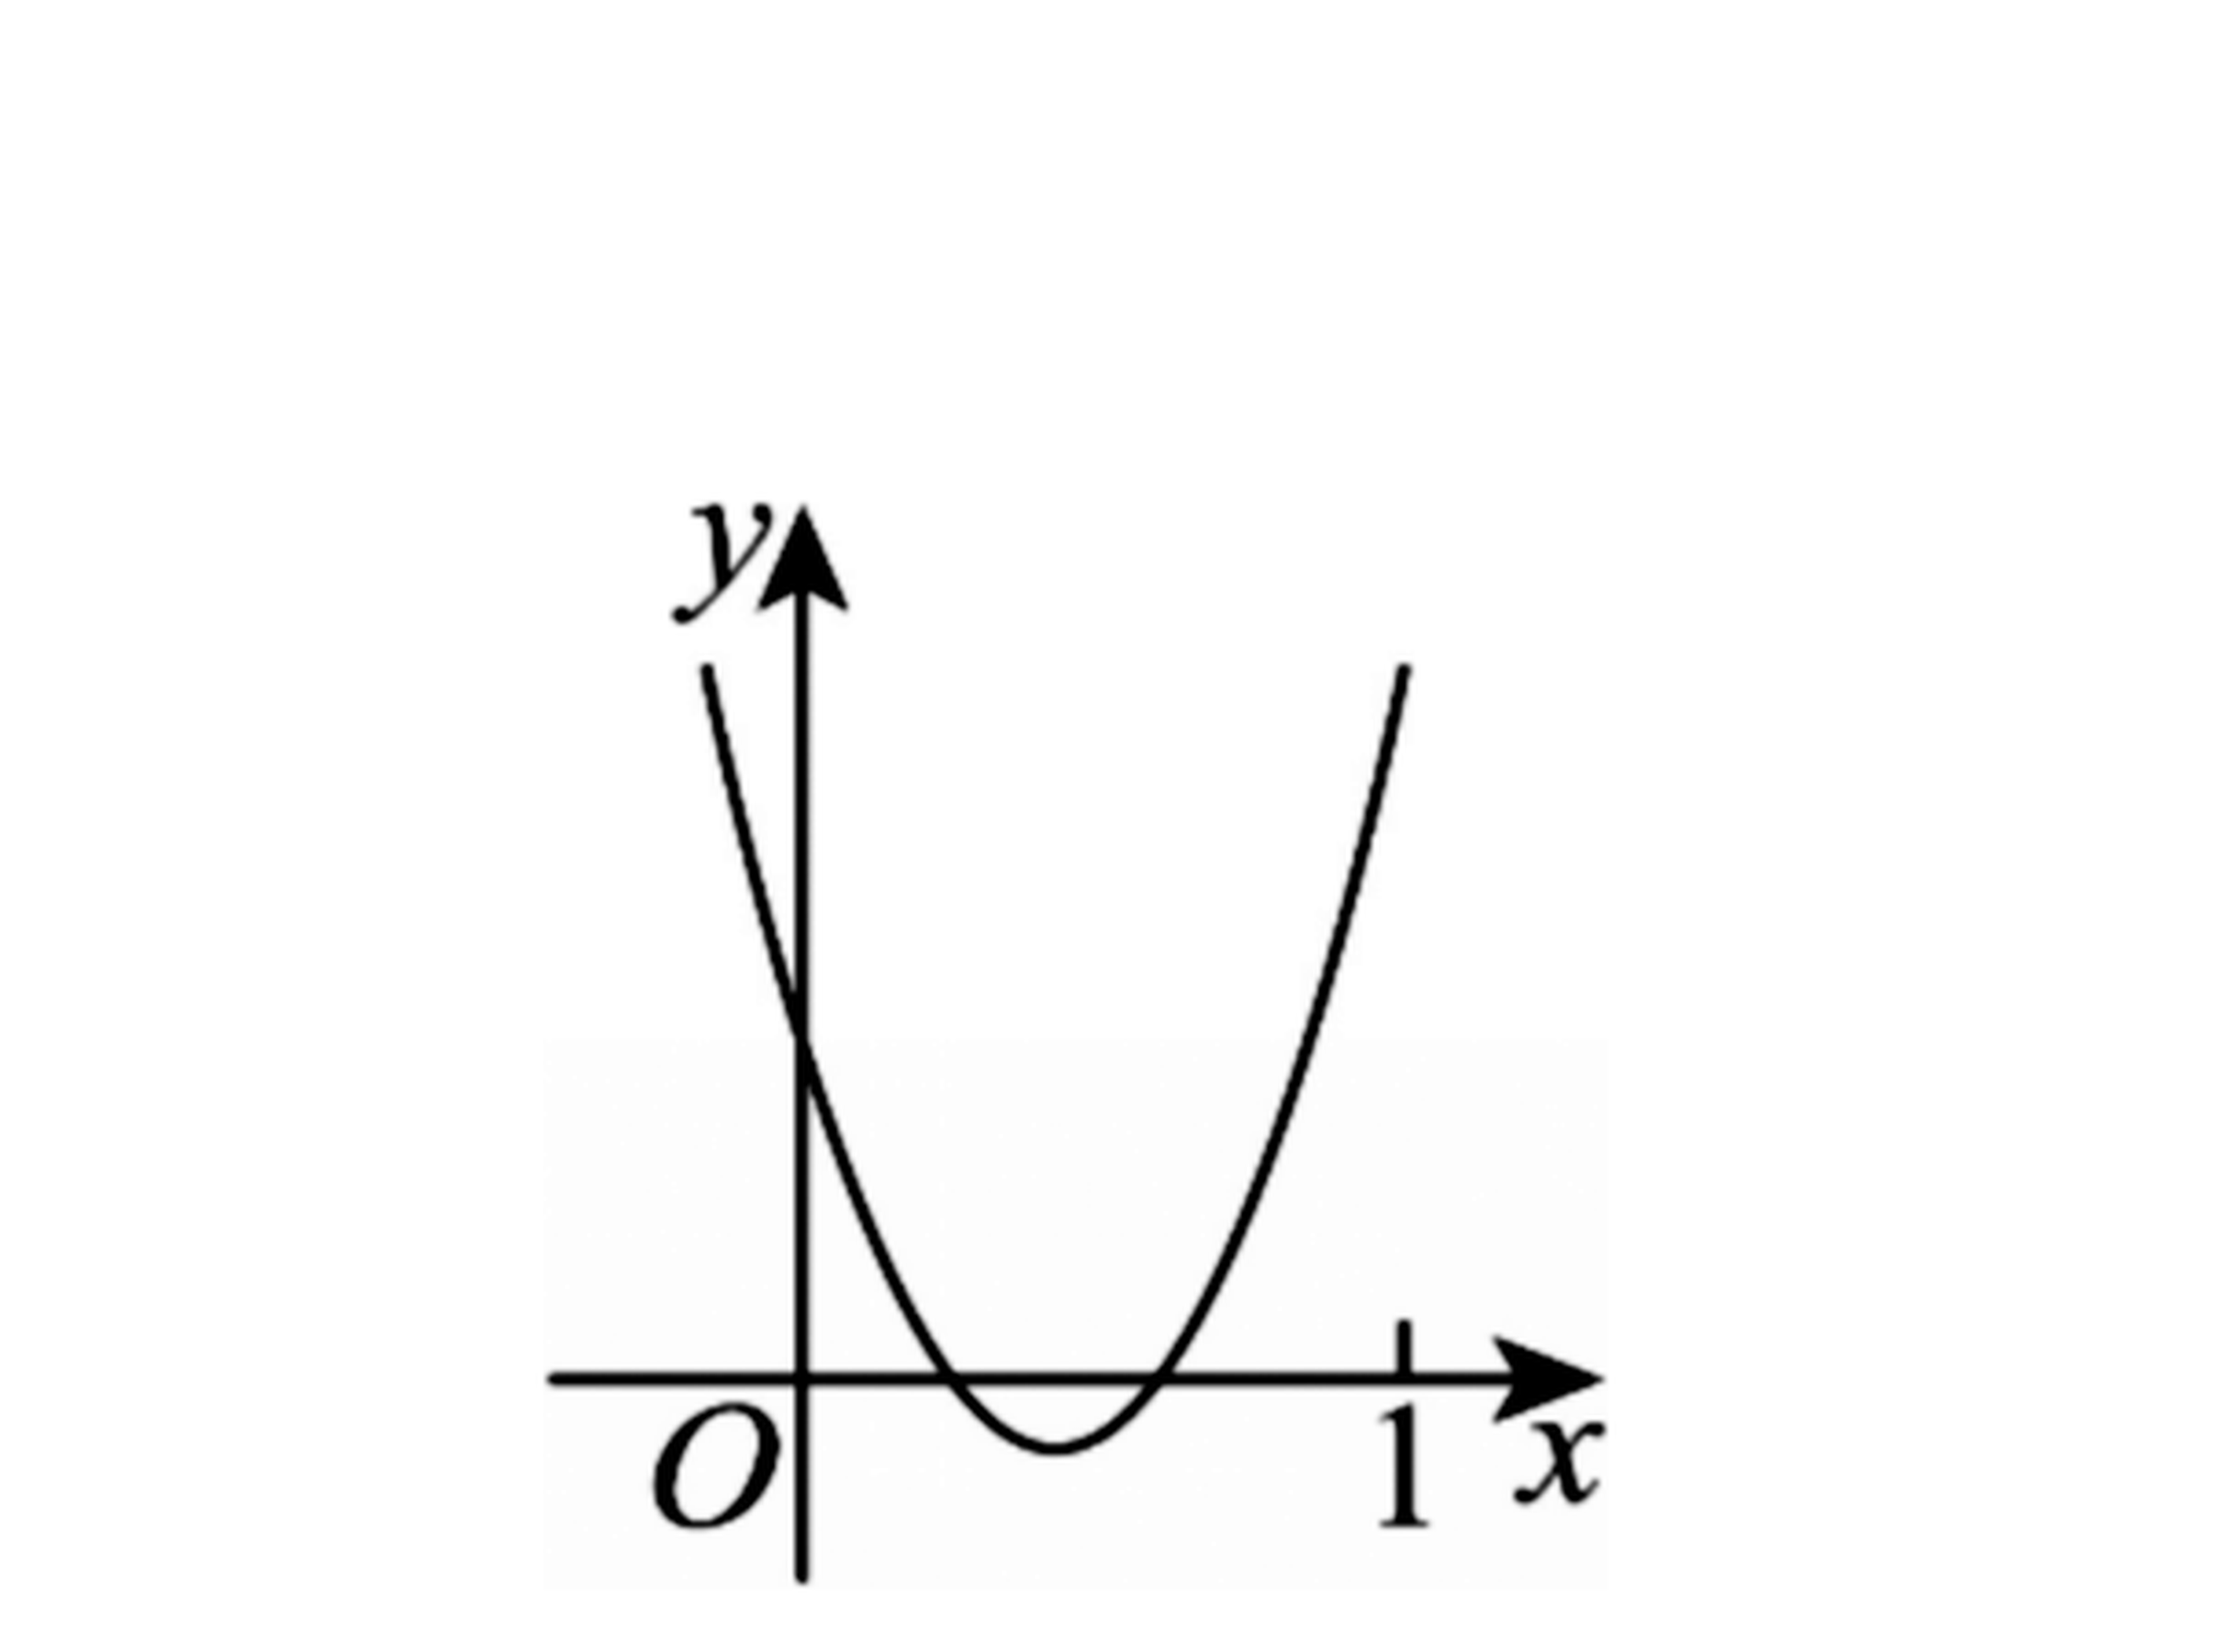
\includegraphics[width=0.32\textwidth]{figures/gao154_q15_stem.png}
\end{center}

\keepwithprev
\begin{center}
% 四幅指数函数图像选项取 05 页上半，按原卷 2×2 排布合并为一张，去粉色水印、去色、4× LANCZOS 放大；三版都出
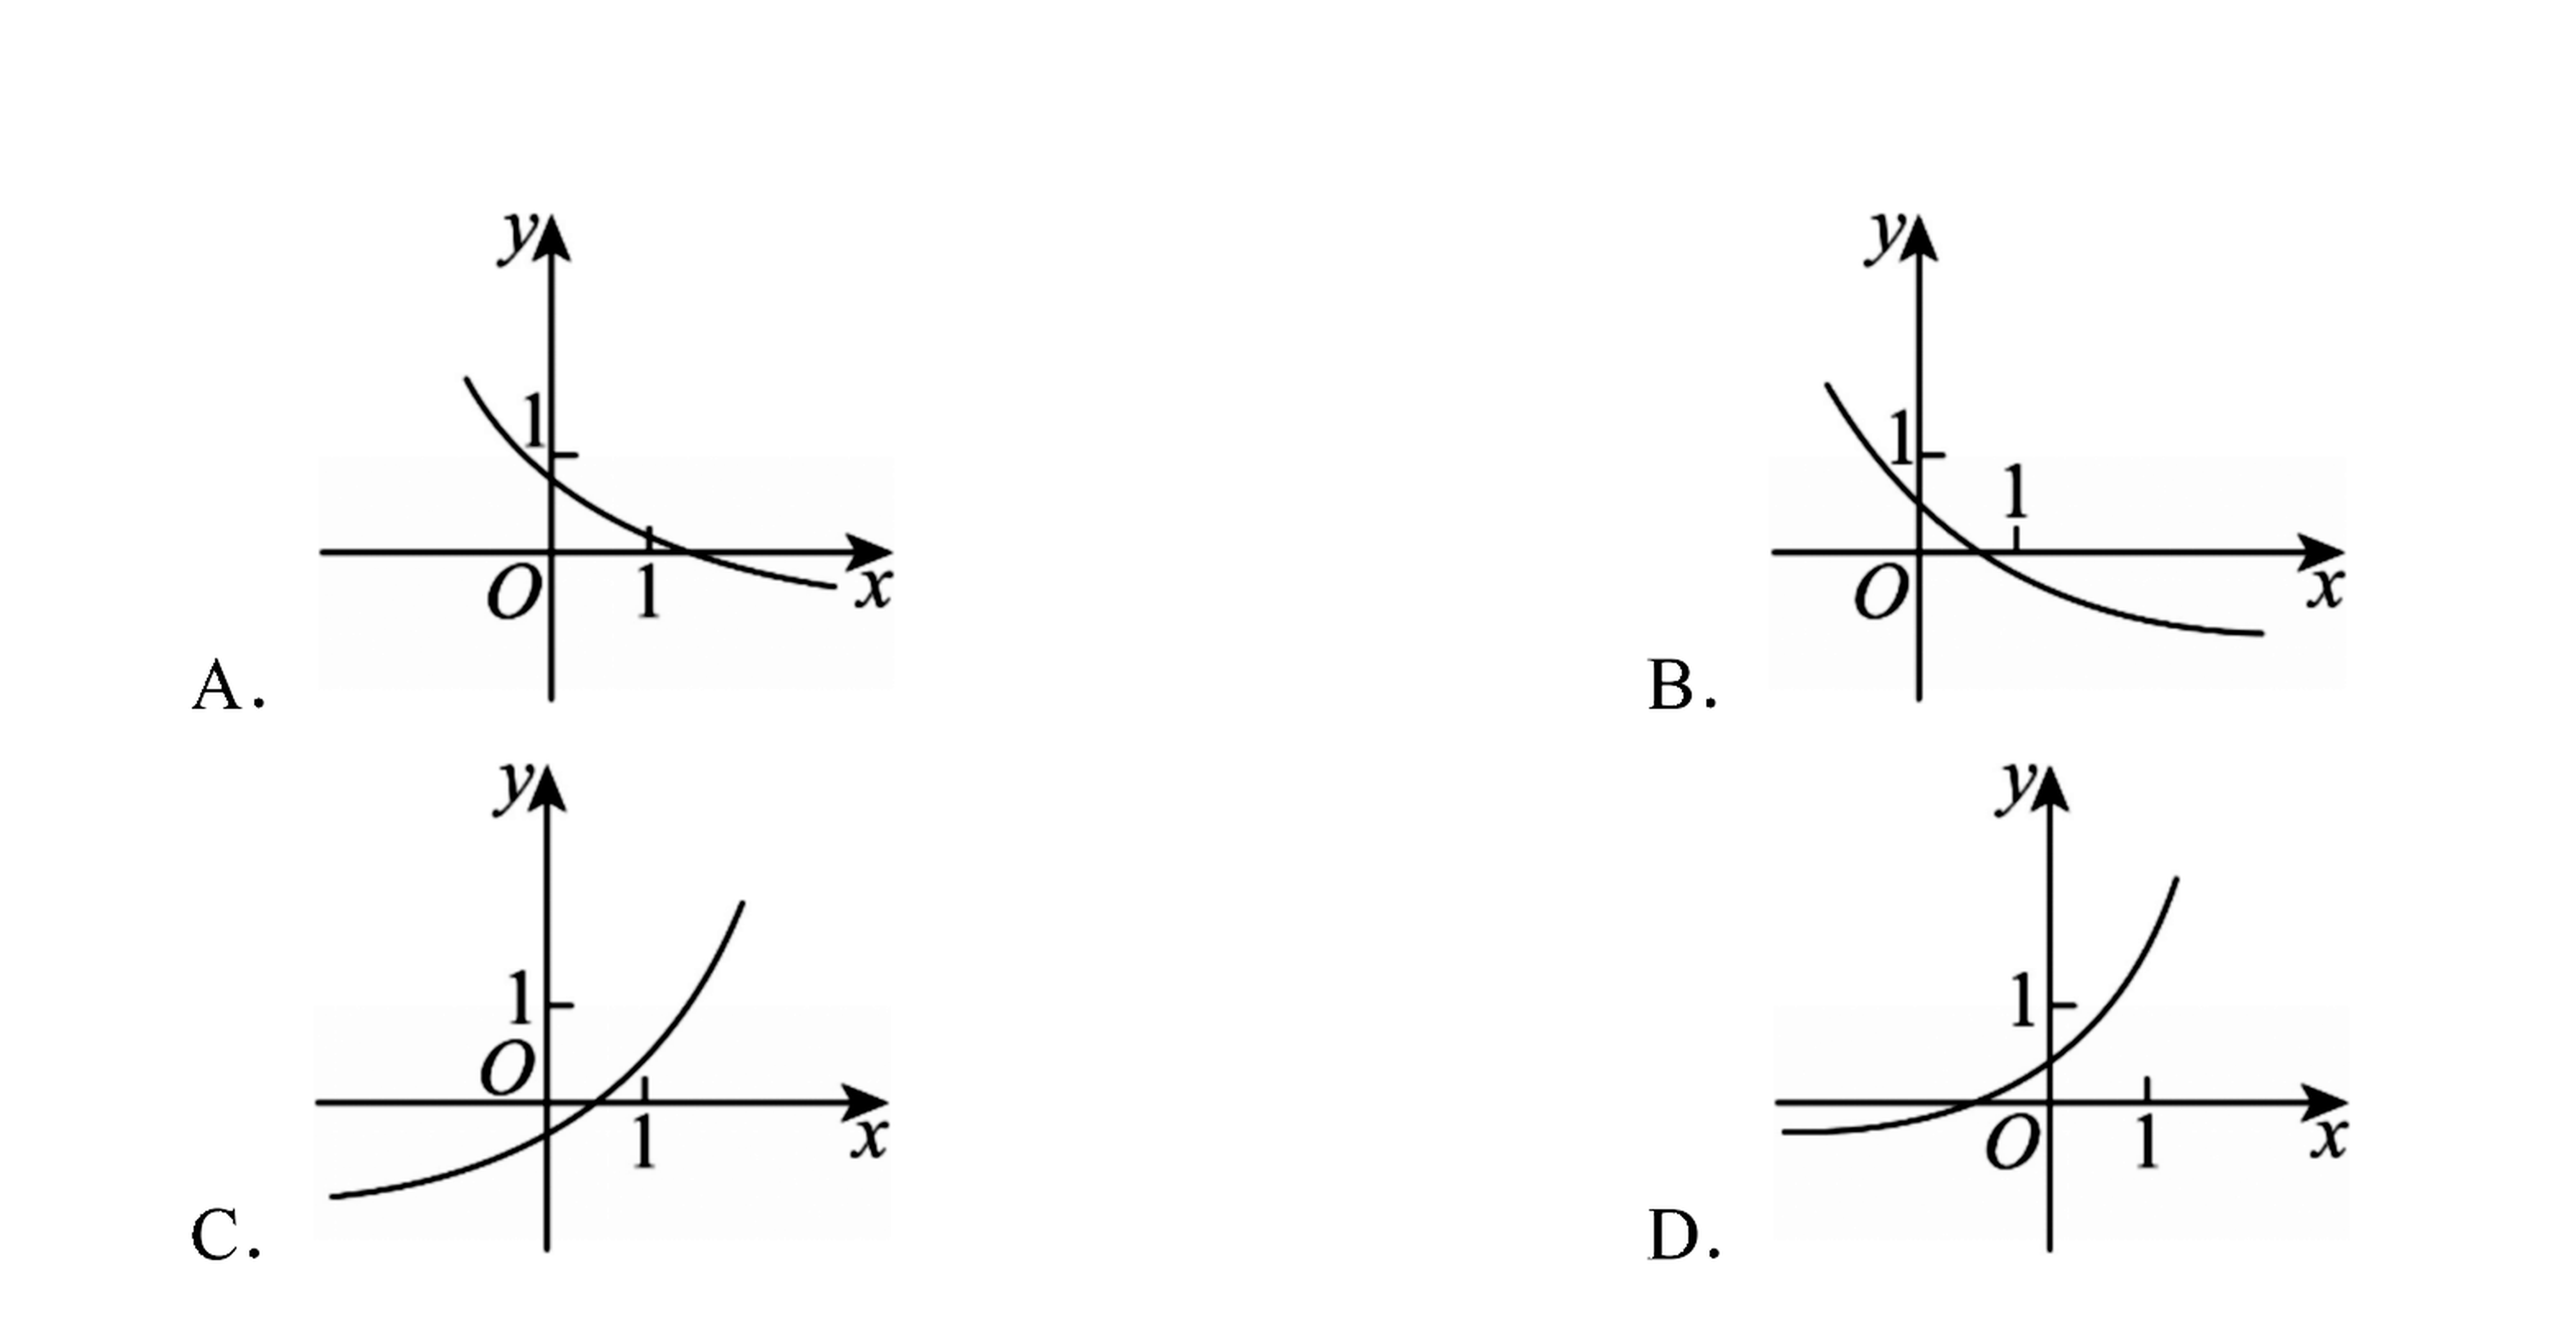
\includegraphics[width=0.80\textwidth]{figures/gao154_q15_opts.png}
\end{center}

\ifanswer
\solbegin
\step{由题意得 $0<a<b<1$，所以 $g(x)=a^x-b$ 在定义域 $\R$ 上严格减.}
\step{$g(0)=a^0-b=1-b>0$，$g(1)=a^1-b=a-b<0$，故 B 符合题意.}
\step{故选 $B$.}
\solend
\fi

% === Q16 === 高斯取整；解析 13 行，故选 C
\item 设 $[a]$ 表示不超过 $a$ 的最大整数，如 $[1.2]=1$，$[-3.2]=-4$，若 $x$、$y$、$z$ 为正实数，则 $\left[\dfrac{y+z}{x}\right]+\left[\dfrac{z+x}{y}\right]+\left[\dfrac{x+y}{z}\right]$ 的最小值为\mbox{（\quad）}

\keepwithprev
A. 2\qquad\qquad B. 3\qquad\qquad C. 4\qquad\qquad D. 6

\ifanswer
\solbegin
\step{若 $x$、$y$、$z$ 为正实数，}
\step{结合基本不等式得 $\dfrac{y+z}{x}+\dfrac{z+x}{y}+\dfrac{x+y}{z}=\dfrac yx+\dfrac xy+\dfrac zx+\dfrac xz+\dfrac zy+\dfrac yz$}
\step{$\geqslant2\sqrt{\dfrac yx\cdot\dfrac xy}+2\sqrt{\dfrac zx\cdot\dfrac xz}+2\sqrt{\dfrac zy\cdot\dfrac yz}=6$，当且仅当 $x=y=z$ 时取等号，}
\step{即 $\dfrac{y+z}{x}$，$\dfrac{z+x}{y}$，$\dfrac{x+y}{z}$ 中至少有一个不小于 2，不妨设 $\dfrac{y+z}{x}\geqslant\dfrac{z+x}{y}\geqslant\dfrac{x+y}{z}$，}
\step{$[a]$ 表示不超过 $a$ 的最大整数和 $\dfrac{y+z}{x}$，$\dfrac{z+x}{y}$，$\dfrac{x+y}{z}$ 中至少有一个不小于 2，}% 原卷此行把两句连写，照录未改（见 ⑤ 3）
\step{得 $\left[\dfrac{y+z}{x}\right]\geqslant2$，所以 $\left[\dfrac{y+z}{x}\right]+\left[\dfrac{z+x}{y}\right]+\left[\dfrac{x+y}{z}\right]\geqslant2$，}
\step{假设 $\left[\dfrac{y+z}{x}\right]+\left[\dfrac{z+x}{y}\right]+\left[\dfrac{x+y}{z}\right]$ 的最小值为 2，$\left[\dfrac{y+z}{x}\right]=2$，$\left[\dfrac{z+x}{y}\right]+\left[\dfrac{x+y}{z}\right]=0$，}
\step{所以 $2\leqslant\dfrac{y+z}{x}<3$，$0<\dfrac{z+x}{y}<1$，$0<\dfrac{x+y}{z}<1$，所以 $2<\dfrac{y+z}{x}+\dfrac{z+x}{y}+\dfrac{x+y}{z}<5$，}
\step{与 $\dfrac{y+z}{x}+\dfrac{z+x}{y}+\dfrac{x+y}{z}\geqslant6$ 矛盾，假设不成立，A 错误；}
\step{假设 $\left[\dfrac{y+z}{x}\right]+\left[\dfrac{z+x}{y}\right]+\left[\dfrac{x+y}{z}\right]$ 的最小值为 3，}
\step{则 $\left[\dfrac{y+z}{x}\right]=2$，$\left[\dfrac{z+x}{y}\right]=1$，$\left[\dfrac{x+y}{z}\right]=0$ 或 $\left[\dfrac{y+z}{x}\right]=3$，$\left[\dfrac{z+x}{y}\right]=\left[\dfrac{x+y}{z}\right]=0$，}
\step{同理可得 $3<\dfrac{y+z}{x}+\dfrac{z+x}{y}+\dfrac{x+y}{z}<6$，显然不成立，B 错误；}
\step{假设 $\left[\dfrac{y+z}{x}\right]+\left[\dfrac{z+x}{y}\right]+\left[\dfrac{x+y}{z}\right]$ 的最小值为 4，易得 $4<\dfrac{y+z}{x}+\dfrac{z+x}{y}+\dfrac{x+y}{z}<7$，}
\step{若取 $x=100$，$y=103$，$z=104$，则 $\left[\dfrac{y+z}{x}\right]=2$，$\left[\dfrac{z+x}{y}\right]=1$，$\left[\dfrac{x+y}{z}\right]=1$，}
\step{即 $\left[\dfrac{y+z}{x}\right]+\left[\dfrac{z+x}{y}\right]+\left[\dfrac{x+y}{z}\right]=4$，假设成立，C 正确，D 错误.}
\step{故选 $C$.}
\solend
\fi

\end{enumerate}

\bigsec{三、解答题}

\begin{enumerate}
\setcounter{enumi}{16}

% === Q17 === $B\subset A$ 单线照录；cases 块；解析 5 行
\item 设集合 $A=\{x\mid x^2+2x-3<0\}$，集合 $B=\{x\mid\lvert x+a\rvert<1\}$.

(1) 若 $a=3$，求 $A\cup B$；

(2) 设命题 $p:x\in A$，命题 $q:x\in B$，若 $p$ 是 $q$ 成立的必要不充分条件，求实数 $a$ 的取值范围.

\ifanswer
\solbegin
\step{(1) $A=(-3,1)$，}
\step{当 $a=3$ 时，$\lvert x+3\rvert<1$，解得 $-4<x<-2$，所以 $B=(-4,-2)$，}
\step{所以 $A\cup B=(-4,1)$.}
\step{(2) 因为 $p$ 是 $q$ 成立的必要不充分条件，所以 $B\subset A$.}
\step{因为 $A=(-3,1)$，$B=(-a-1,-a+1)$，所以 $\begin{cases}-a-1\geqslant-3\\-a+1<1\end{cases}$ 或 $\begin{cases}-a-1>-3\\-a+1\leqslant1\end{cases}$，解得 $0\leqslant a\leqslant2$.}
\solend
\fi

% === Q18 === 判别式 \Delta 两处照录；解析 9 行
\item 已知关于 $x$ 的一元二次方程 $x^2-mx+4m^2-3=0$ 的两个实根分别为 $x_1,x_2$.

(1) 若 $x_1,x_2$ 满足 $x_1+x_2=x_1x_2$，求实数 $m$ 的值；

(2) 求 $x_1^2+x_2^2$ 的最小值.

\ifanswer
\solbegin
\step{(1) 由韦达定理 $x_1+x_2=m$，$x_1x_2=4m^2-3$，}
\step{$\Delta=m^2-4(4m^2-3)=-15m^2+12\geqslant0$，即 $m^2\leqslant\dfrac45$.}
\step{由 $x_1+x_2=x_1x_2$ 得 $m=4m^2-3$，即 $4m^2-m-3=0$，}
\step{解得 $m=1$ 或 $m=-\dfrac34$.}
\step{$m=1$ 时 $m^2=1>\dfrac45$，$\Delta<0$，舍去；}
\step{$m=-\dfrac34$ 时 $m^2=\dfrac9{16}<\dfrac45$，符合，故 $m=-\dfrac34$.}
\step{(2) $x_1^2+x_2^2=(x_1+x_2)^2-2x_1x_2=m^2-2(4m^2-3)=-7m^2+6$，}
\step{函数 $y=-7m^2+6$ 开口向下，对称轴为 $m=0$，}% 原卷此处称求「最小值」，实为闭区间 $m^2\le\frac45$ 上的最小值，照录未改（见 ⑤ 4）
\step{故 $y_{\min}=-7\cdot\dfrac45+6=-\dfrac{28}{5}+\dfrac{30}{5}=\dfrac25$.}
\solend
\fi

% === Q19 === 全称命题；cases 块；解析 9 行
\item 设命题 $p$：对任意 $x\in\R$，不等式 $2mx^2+2mx+1>0$ 恒成立，$q:m\in\{m\mid\log_2(m-1)<1\}$.

(1) 若 $p$ 为真命题，求实数 $m$ 的取值范围；

(2) 若命题 $p$、$q$ 有且只有一个是真命题，求实数 $m$ 的取值范围.

\ifanswer
\solbegin
\step{(1) 由 $p$ 为真命题，得 $\forall x\in\R$，不等式 $2mx^2+2mx+1>0$ 恒成立，}
\step{当 $m=0$ 时，$1>0$ 恒成立；}
\step{当 $m\ne0$ 时，$\begin{cases}2m>0\\\Delta=4m^2-8m<0\end{cases}$，解得 $0<m<2$；}
\step{综上，$0\leqslant m<2$，即 $m$ 的取值范围是 $[0,2)$；}
\step{(2) 若 $q$ 为真，则有 $\log_2(m-1)<1$，得 $0<m-1<2$，解得 $1<m<3$，}
\step{因此命题 $q:m\in\{m\mid1<m<3\}$，由 (1) 得命题 $p:\{m\mid0\leqslant m<2\}$，}
\step{而命题 $p$、$q$ 有且只有一个是真命题，}
\step{当 $p$ 真 $q$ 假时，$\begin{cases}0\leqslant m<2\\m\leqslant1\text{ 或 }m\geqslant3\end{cases}$，解得 $0\leqslant m\leqslant1$，}
\step{当 $p$ 假 $q$ 真时，$\begin{cases}m<0\text{ 或 }m\geqslant2\\1<m<3\end{cases}$，解得 $2\leqslant m<3$，}
\step{故实数 $m$ 的取值范围是 $\{m\mid0\leqslant m\leqslant1\text{ 或 }2\leqslant m<3\}$.}
\solend
\fi

% === Q20 === Labubu 成本题；解析 10 行
\item Labubu 公司拟在 2027 年初推出智能机器人系列玩偶（单位：套）. 根据以往经验，其中一条生产线每月生产 $x$ 套玩具的成本 $P$ 由两部分费用（单位：元）构成：

(i) 固定成本（与生产玩具套数 $x$ 无关），总计 160000 元；

(ii) 每生产 $x$ 套需另投入的生产成本 $c(x)$ 元，其中 $c(x)=10x+\dfrac1{100}x^2$.

(1) 假设该生产线每月生产出的玩具能全部售出，问：该生产线每月生产玩具多少套时，可使得平均每套所需成本费用最少？此时每套玩具的成本费用是多少？

(2) 假设该生产线每月生产出的玩具能全部售出，但随着 $x$ 的增大，每月生产所需的直接总成本在急剧增加，因此售价也需随着 $x$ 的增大而适当增加. 设每套玩具的售价为 $q(x)$ 元，$q(x)=a+\dfrac xb$（$a,b\in\R$）. 若当月产量为 10000 套时利润最大，此时每套售价为 150 元，试求 $a,b$ 的值.（利润=销售收入$-$成本费用）

\ifanswer
\solbegin
\step{(1) 每月总成本 $P=160000+10x+\dfrac1{100}x^2$，}
\step{平均每套成本为 $\dfrac Px=\dfrac{160000}{x}+10+\dfrac x{100}\geqslant10+2\sqrt{\dfrac{160000}{x}\cdot\dfrac x{100}}=90$.}
\step{等号成立当且仅当 $\dfrac{160000}{x}=\dfrac x{100}$ 时，即 $x=4000$ 时取等号，}
\step{所以每月生产 4000 套时平均每套成本最少，此时每套成本为 90 元.}
\step{(2) 利润 $W(x)=x\cdot q(x)-P=\left(\dfrac1b-\dfrac1{100}\right)x^2+(a-10)x-160000$.}
\step{要在 $x=10000$ 处取得最大值，需 $\dfrac1b-\dfrac1{100}<0$，且对称轴为 $x=10000$，}
\step{故 $-\dfrac{a-10}{2\left(\frac1b-\frac1{100}\right)}=10000$，即 $a-10=-20000\left(\dfrac1b-\dfrac1{100}\right)$.}
\step{又 $q(10000)=a+\dfrac{10000}{b}=150$.}
\step{令 $t=\dfrac1b$，则 $a=150-10000t$，}
\step{代入上式 $140-10000t=-20000t+200$，解得 $t=\dfrac3{500}$，即 $b=\dfrac{500}{3}$；}
\step{再由 $a=150-10000\times\dfrac3{500}=150-60=90$，所以 $a=90$，$b=\dfrac{500}{3}$.}
\solend
\fi

% === Q21 === $A^+$／$A^-$ 新定义；$A\subseteq$ 带下划线照录、\varnothing；解析 16 行
\item 设集合 $A$ 为非空数集，定义 $A^+=\{x\mid x=a+b,a,b\in A\}$，$A^-=\{x\mid x=\lvert a-b\rvert,a,b\in A\}$.

(1) 若集合 $A=\{-1,1\}$，写出集合 $A^+$ 及 $A^-$；

(2) 若集合 $A=\{x_1,x_2,x_3,x_4\}$，$x_1<x_2<x_3<x_4$，且 $A^-=A$，求证：$x_1+x_4=x_2+x_3$；

(3) 若集合 $A\subseteq\{x\mid0\leqslant x\leqslant2020,x\in\N\}$，且 $A^+\cap A^-=\varnothing$，求集合 $A$ 元素的个数的最大值.

\ifanswer
\solbegin
\step{(1) 由 $A=\{-1,1\}$，得 $A^+=\{-2,0,2\}$，$A^-=\{0,2\}$；}
\step{(2) 由于集合 $A=\{x_1,x_2,x_3,x_4\}$，$x_1<x_2<x_3<x_4$，且 $A^-=A$，}
\step{所以 $A^-$ 中也只包含四个元素，即 $A^-=\{0,x_2-x_1,x_3-x_1,x_4-x_1\}$，}
\step{剩下的 $x_3-x_2=x_4-x_3=x_2-x_1$，所以 $x_1+x_4=x_2+x_3$；}
\step{(3) 设 $A=\{a_1,a_2,\cdots,a_k\}$ 满足题意，其中 $a_1<a_2<\cdots<a_k$，}
\step{则 $2a_1<a_1+a_2<a_1+a_3<\cdots<a_1+a_k<a_2+a_k<a_3+a_k<\cdots<a_{k-1}+a_k<2a_k$，所以 $\lvert A^+\rvert\geqslant2k-1$，}
\step{且 $a_1-a_1<a_2-a_1<a_3-a_1<\cdots<a_k-a_1$，所以 $\lvert A^-\rvert\geqslant k$，}
\step{因为 $A^+\cap A^-=\varnothing$，所以 $\lvert A^+\cup A^-\rvert=\lvert A^+\rvert+\lvert A^-\rvert\geqslant3k-1$，}
\step{$A^+\cup A^-$ 中最小的元素为 0，最大的元素为 $2a_k$，所以 $\lvert A^+\cup A^-\rvert\leqslant2a_k+1$，}
\step{所以 $3k-1\leqslant2a_k+1\leqslant4041$（$k\in\N^*$），所以 $k\leqslant1347$，}
\step{实际上当 $A=\{674,675,676,\cdots,2020\}$ 时满足题意，证明如下：}
\step{设 $A=\{m,m+1,m+2,\cdots,2020\}$，$m\in\N$，}
\step{则 $A^+=\{2m,2m+1,2m+2,\cdots,4040\}$，$A^-=\{0,1,2,\cdots,2020-m\}$，}
\step{由题意得 $2020-m<2m$，即 $m>673\dfrac13$，}
\step{故 $m$ 的最小值为 674，于是当 $m=674$ 时，$A$ 中元素最多，}
\step{即 $A=\{674,675,676,\cdots,2020\}$ 时满足题意，}
\step{综上所述，集合 $A$ 中元素的个数的最大值是 1347.}
\solend
\fi

\end{enumerate}

\bigsec{附加题}

\begin{enumerate}

% === 附加题 1 === 另起编号 1；「n 元集和集」弯引号；解析 6 行
\item 设集合 $A=\{a_1,a_2,a_3,a_4\}$，$C=\{2,3,4,6\}$，新定义：集合 $A$ 中所有含 $n$ 个元素的子集中 $n$ 个元素之和的不同值组成的集合为“$n$ 元集和集”. 若 $A$ 的“3 元集和集”为 $C$，则集合 $A=$\blankline[4.4em].

\ifanswer
\solbegin
\step{集合 $A$ 的 3 元子集共有 4 个：$\{a_1,a_2,a_3\}$，$\{a_1,a_2,a_4\}$，$\{a_1,a_3,a_4\}$，$\{a_2,a_3,a_4\}$，}
\step{集合 $C=\{a_1+a_2+a_3,a_1+a_2+a_4,a_1+a_3+a_4,a_2+a_3+a_4\}$，}
\step{不妨令 $a_1<a_2<a_3<a_4$，}
\step{则 $a_1+a_2+a_3<a_1+a_2+a_4<a_1+a_3+a_4<a_2+a_3+a_4$，}
\step{而 $C=\{2,3,4,6\}$，因此 $\begin{cases}a_1+a_2+a_3=2\\a_1+a_2+a_4=3\\a_1+a_3+a_4=4\\a_2+a_3+a_4=6\end{cases}$，相加化简得 $a_1+a_2+a_3+a_4=5$，}
\step{解得 $a_1=-1$，$a_2=1$，$a_3=2$，$a_4=3$，所以 $A=\{-1,1,2,3\}$.}
\solend
\fi

% === 附加题 2 === 解析配图（仅答案版出）；四选项；解析 15 行，故选 A
\item 已知函数 $f(x)=\log_p x+q$，其中 $p>0$ 且 $p\ne1$，曲线 $y=f(x)$ 经过 $P(1,2)$、$Q(2,3)$ 两点. 设 $g(x)=f(x)\cdot[f(x)-2]$，若 $\lvert g(a)\rvert=\lvert g(b)\rvert=\lvert g(c)\rvert=\lvert g(d)\rvert$，且 $a<b<c<d$，则 $ad(b+c)$ 的取值范围为\mbox{（\quad）}

\keepwithprev
A. $\left(\dfrac14,\dfrac5{16}\right)$\qquad B. $\left(\dfrac18,\dfrac5{16}\right)$\qquad C. $\left(\dfrac14,\dfrac25\right)$\qquad D. $\left(\dfrac18,\dfrac25\right)$

\ifanswer
\solbegin
\step{函数 $f(x)=\log_p x+q$，且曲线 $y=f(x)$ 经过点 $P(1,2)$ 和 $Q(2,3)$，}
\step{所以 $\begin{cases}f(1)=q=2\\f(2)=\log_p2+q=3\end{cases}$，解得 $p=2$，$q=2$，$f(x)=\log_2 x+2$.}
\step{不妨设 $\lvert g(x)\rvert=k$，令 $\log_2 x=m$，则 $f(x)\cdot[f(x)-2]=m(m+2)=m^2+2m$，}
\step{画出函数 $y=\lvert m^2+2m\rvert$ 的图象，如图所示，}
\begin{center}
% $y=|m(m+2)|$ 图像取 11 页右上，去粉色水印、去色、4× LANCZOS 放大；仅答案版出
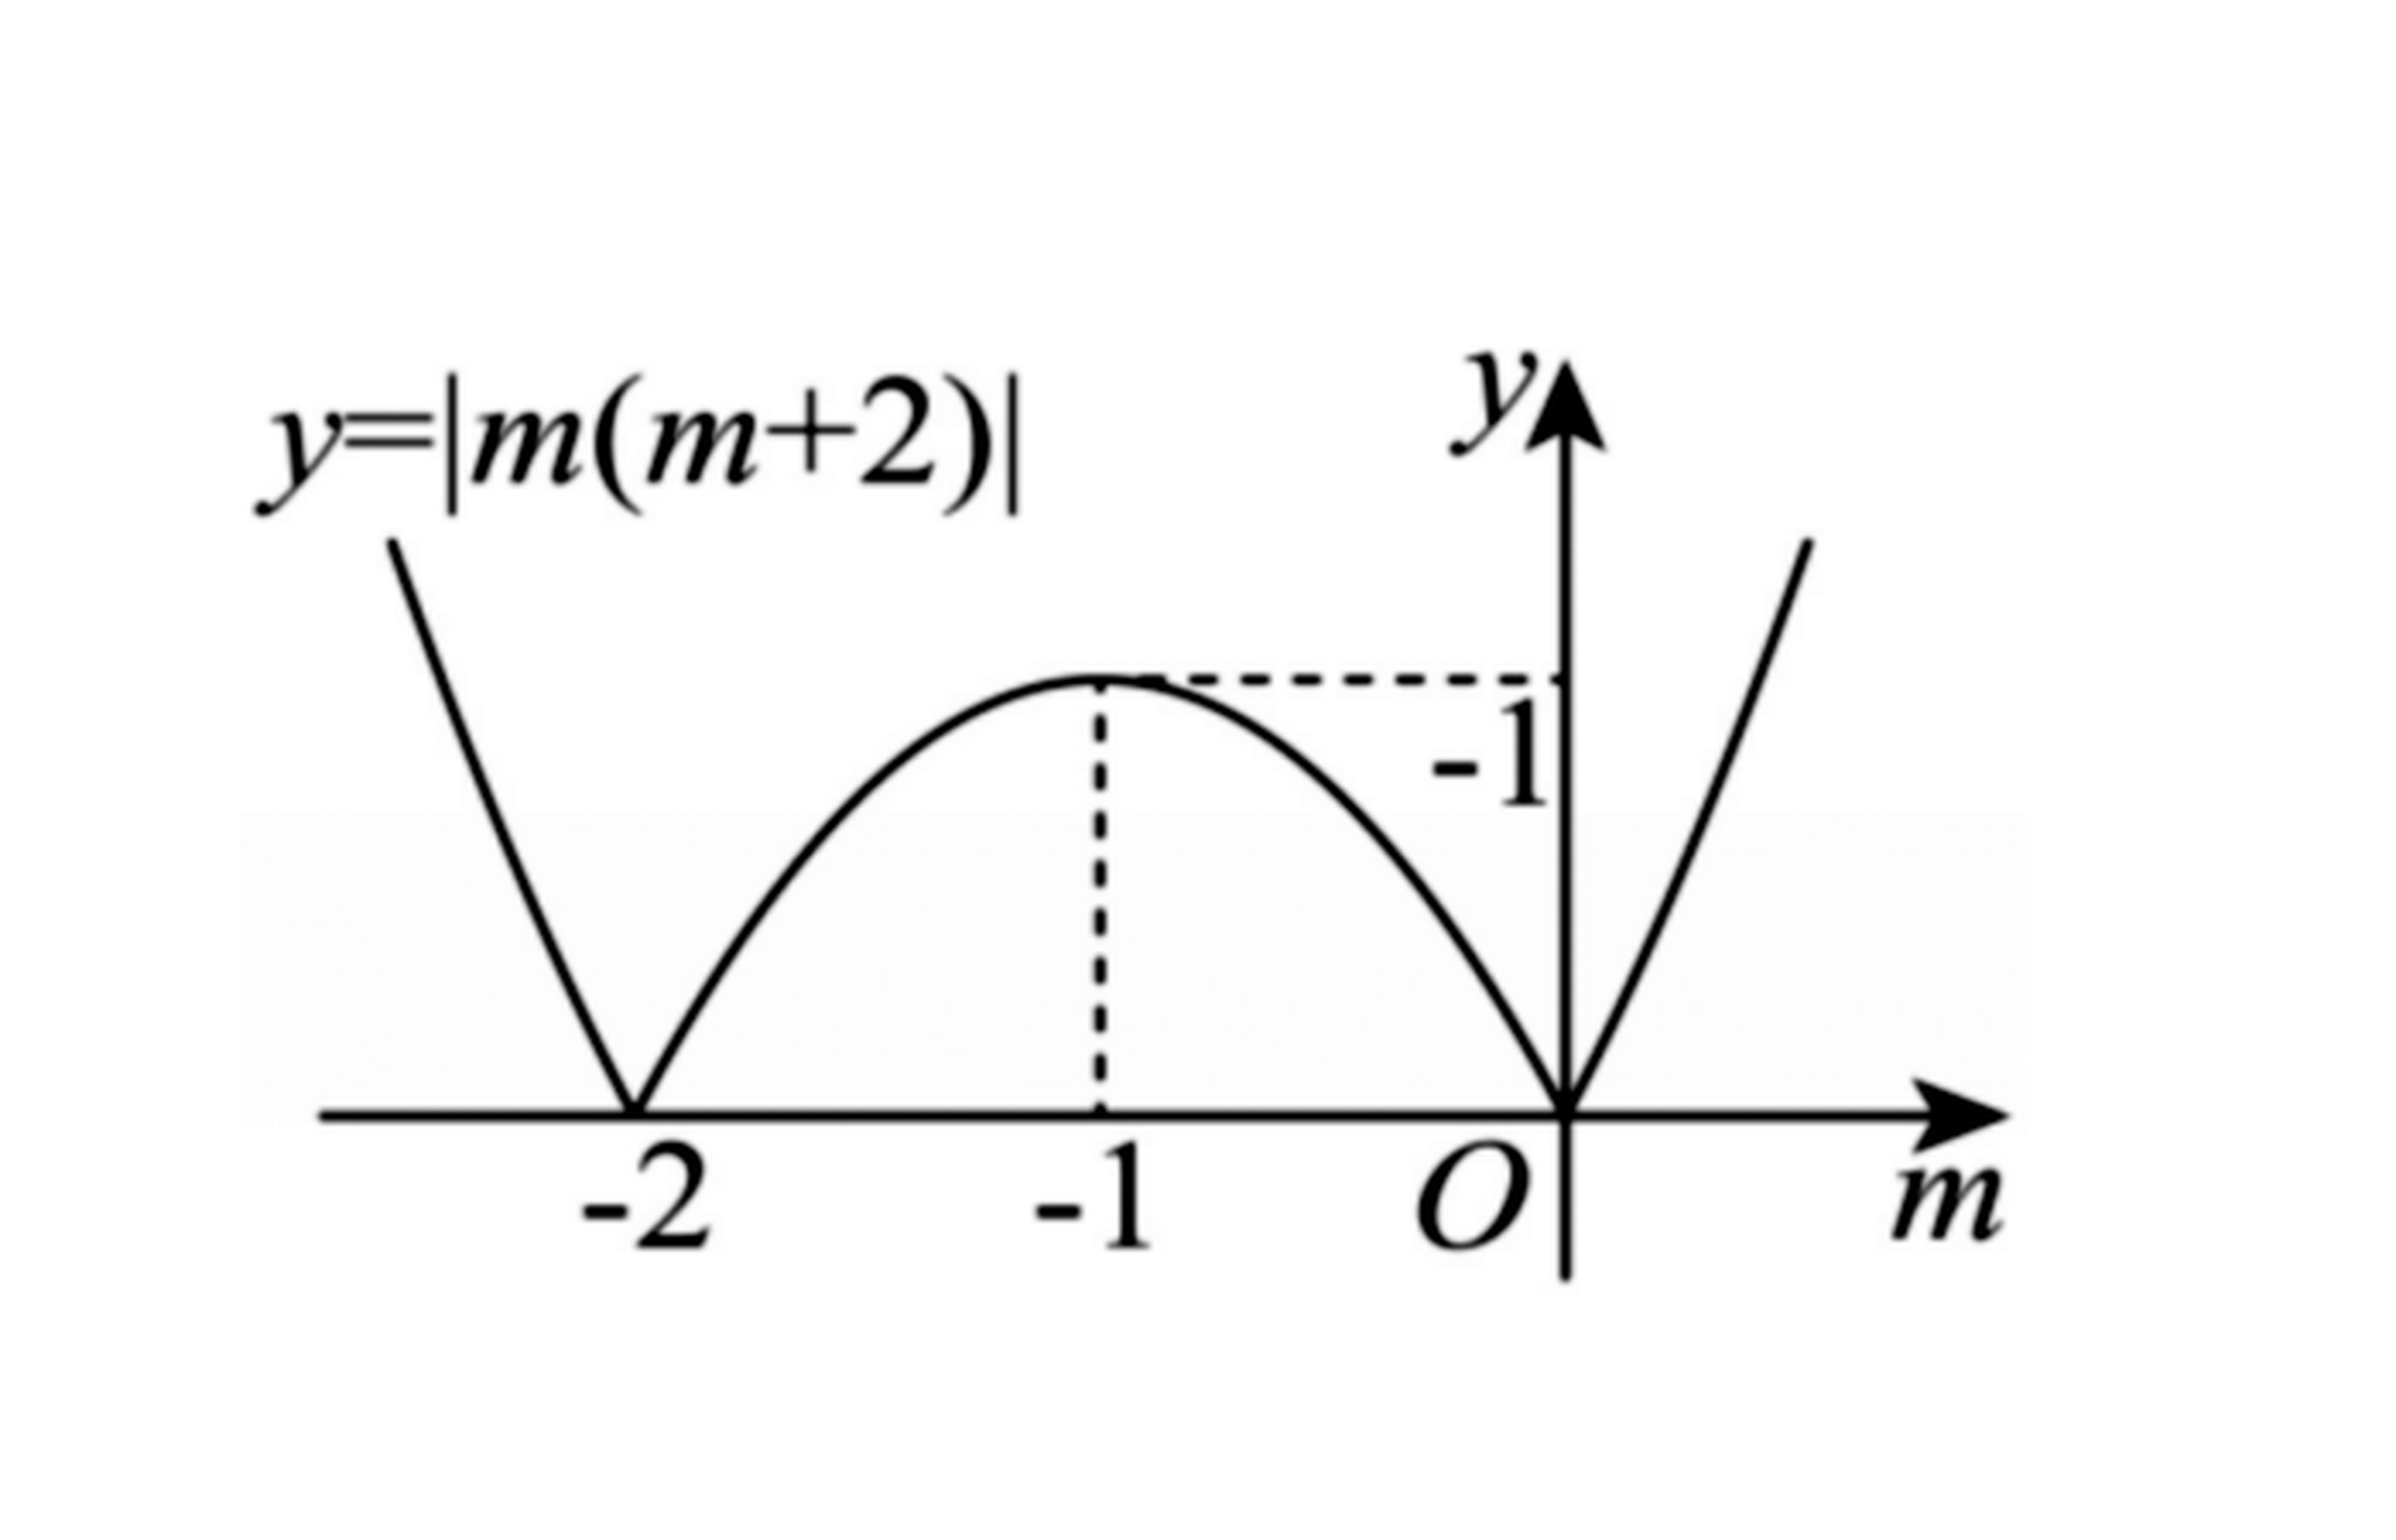
\includegraphics[width=0.46\textwidth]{figures/gao154_fujia2.png}
\end{center}
\step{由图像得 $k\in(0,1)$，}
\step{所以方程 $m^2+2m=k$ 和 $m^2+2m=-k$ 各有两个不同的根，}
\step{其中方程 $m^2+2m-k=0$ 的两根为 $m=-1\pm\sqrt{1+k}$，}
\step{方程 $m^2+2m+k=0$ 的两根为 $m=-1\pm\sqrt{1-k}$，}
\step{所以 $m_1=-1-\sqrt{1+k}$，$m_2=-1-\sqrt{1-k}$，$m_3=-1+\sqrt{1-k}$，$m_4=-1+\sqrt{1+k}$，且 $m_1<m_2<m_3<m_4$，}
\step{由 $m=\log_2 x$，则 $x=2^m$，}
\step{所以 $a=2^{-1-\sqrt{1+k}}$，$b=2^{-1-\sqrt{1-k}}$，$c=2^{-1+\sqrt{1-k}}$，$d=2^{-1+\sqrt{1+k}}$，}
\step{所以 $ad=2^{-1-\sqrt{1+k}}\times2^{-1+\sqrt{1+k}}=2^{(-1-\sqrt{1+k})+(-1+\sqrt{1+k})}=2^{-2}=\dfrac14$，}
\step{$b+c=2^{-1-\sqrt{1-k}}+2^{-1+\sqrt{1-k}}=\dfrac{2^{-\sqrt{1-k}}+2^{\sqrt{1-k}}}{2}$，}
\step{令 $s=\sqrt{1-k}$，其中 $s\in(0,1)$，则 $b+c=\dfrac12\left(2^{-s}+2^s\right)$，}
\step{设函数 $y=2^s+\dfrac1{2^s}$，令 $r=2^s\in(1,2)$，所以 $y=r+\dfrac1r$ 在 $(1,2)$ 上严格增，}
\step{所以函数 $y=2^s+\dfrac1{2^s}$ 在 $(0,1)$ 上严格增，所以 $y=2^s+\dfrac1{2^s}\in\left(2,\dfrac52\right)$，}
\step{所以 $b+c=\dfrac{2^{-s}+2^s}{2}\in\left(1,\dfrac54\right)$，$ad(b+c)=\dfrac{b+c}{4}\in\left(\dfrac14,\dfrac5{16}\right)$，}
\step{所以 $ad(b+c)$ 的取值范围是 $\left(\dfrac14,\dfrac5{16}\right)$，故选 $A$.}
\solend
\fi

\end{enumerate}

\end{document}
"
% 紧凑版：xelatex "\def\iscompact{1}% 高一154_徐汇中学_期中.tex
%   —— 高一上数学"2026-2027 年徐汇中学高一上期中"（试卷版/答案版/紧凑版）
% 试卷版：xelatex 高一154_徐汇中学_期中.tex
% 答案版：xelatex "\def\isanswer{1}% 高一154_徐汇中学_期中.tex
%   —— 高一上数学"2026-2027 年徐汇中学高一上期中"（试卷版/答案版/紧凑版）
% 试卷版：xelatex 高一154_徐汇中学_期中.tex
% 答案版：xelatex "\def\isanswer{1}\input{高一154_徐汇中学_期中.tex}"
% 紧凑版：xelatex "\def\iscompact{1}\input{高一154_徐汇中学_期中.tex}"
%
% ① 原始材料：微信公众号"魔都数学加油站"文章，连载"27学年高一154"，原文标题
% "27学年高一154——2026-2027年上海市徐汇中学高一上期中"；
% 原文链接：https://mp.weixin.qq.com/s/Qs2T7Zwsug-KKFE2wefDUg 。
% 正文为 12 张 PNG 页（01/03/04/05/07/11/12 为 2560×3620，
% 02/06/08/09/10 为 4762×6735，同一篇各页分辨率混排，逐页按各自分辨率裁图核对）。
% 体例：讲评版——一、填空题 3—12（10 题）、二、选择题 13—16（4 题）、
% 三、解答题 17—21（5 题）、附加题 1—2（2 题，原卷**另起编号**"1." "2."，
% 不与正题连号，同 高一a 成例），共 21 题；全卷每题均印【解析】
% （逐题核实，见 ② ②）。题目、答案、解析均据原图转录；卷面粉红色水印
% "魔都数学加油站"及公众号页脚未录入。
% 全卷插图清单（逐页通读 12 页确认）：3 组——
%   · Q15 题干配图（$f(x)=(x-a)(x-b)$ 抛物线，04 页右下：x/y 轴、O、1、
%     开口向上两零点均在 (0,1) 内），三版都出，裁 figures/gao154_q15_stem.png；
%   · Q15 四幅图像选项（05 页上半 2×2 排布，A/B/C/D 四幅指数函数图像，
%     合并成一张，照 高一136 Q13/Q22 成例），三版都出，
%     裁 figures/gao154_q15_opts.png；
%   · 附加题第 2 题解析配图（$y=\lvert m(m+2)\rvert$ 图像，11 页右上：
%     W 形折线、$-2$、$-1$、O、虚线 $y=1$ 与 $m=-1$），仅答案版出，
%     裁 figures/gao154_fujia2.png；
%   3 图均取自原卷截图，去粉色水印、去色、4× LANCZOS 放大；Q15 题干图
%   左侧题干残字"的图"已裁白。其余各页逐页确认无其它题目配图、无表格；
%   12 页下半仅水印、无正文。
%
% 卷首标题：原卷印作"2026-2027 年徐汇中学高一上期中"，年份区间按全稿惯例排 en dash；
% 原卷卷面未印副标题，本稿按同期中卷知识模块口径补出"集合与常用逻辑用语、不等式、函数"。
%
% ② 与原卷的排版差异：
%   ① 原文从第 3 题起，本稿保留原题号；共 21 题四节，正题到 21，附加题另起编号
%      1—2（\bigsec{附加题} 后 \begin{enumerate} 不 \setcounter，同 高一a 成例）；
%   ② 全 21 题均印【解析】、用 \solbegin…\solend，无只印【答案】或答案印括号内的题；
%      四道正题选择题答案在解析末句"故选 C／A／B／C"（Q13—Q16）、附加题第 2 题
%      答案在解析末句"故选 A"，括号 \mbox{（\quad）} 留空、不另提 \ans{}；
%      答案版【答案】/【解析】标记数 = 21 = 全卷题数；
%   ③ 原卷卷面未印副标题，本稿按知识模块口径补出；
%   ④ 原卷填空横线按全稿惯例排 \blankline[4.4em]；选择题括号排 \mbox{（\quad）}、
%      四道正题选择题与附加题第 2 题的选项段前按惯例各加 \keepwithprev
%      （Q15 与附加题 2 的选项段是整块图，\keepwithprev 后接 \begin{center}）；
%      解答题不留作答区、不加 \anspace（原卷为讲评版）；
%   ⑤ 数集黑板粗体：Q4"$x,y\in R$"、Q9"$x\in\R$"、Q13 无、
%      Q15"定义域 $\R$"、Q19"$\forall x\in\R$"、Q21"$x\in\N$"与"$k\in\N^*$"、
%      Q20"$a,b\in\R$"、附加题 2 无——原卷印斜体或正体粗体 R/N/N*，
%      按全稿惯例归一 \R／\N／\N^*；绝对值排 \lvert…\rvert
%      （Q5、Q9、Q12、Q13、Q16、Q21、附加题 2），集合描述竖线排 \mid
%      （Q5、Q17、Q19、Q21），不等号按全稿惯例排 \leqslant／\geqslant；
%      空集 \varnothing（Q21 题干 (3)）；
%   ⑥ 子集符号逐处照录、不得统一：Q6 题干印"$\{1,2\}\subset M\subseteq\{1,2,3,4,5\}$"
%      （前单线 ⊂、后带下划线 ⊆，同句两形并用），解析亦两形并用；
%      Q17 解析 (2)"$B\subset A$"印单线 ⊂；Q21 题干 (3)"$A\subseteq\{x\mid\cdots\}$"
%      印带下划线 ⊆——逐处放大核，分别 \subset／\subseteq，照录未统一（见 ④）；
%   ⑦ 判别式 Δ/△：Q18 解析 (1)"$\Delta=m^2-4(4m^2-3)$"与 Q19 解析 (1)
%      "$\Delta=4m^2-8m<0$"两处均印等腰偏高粗三角、照录 \Delta；本卷无扁等边
%      细线 \triangle 用例（见 ④）；
%   ⑧ 中文弯引号照录：Q4"设 $x$、$y\in\R$. 若 $x+y>2$，则 $x>1$ 或 $y>1$"、
%      附加题 1"$n$ 元集和集"与"3 元集和集"；注释里一律 ASCII 引号；
%      数学式内 CJK 用 \text{}（Q5 解集描述"或"、Q19 集合描述的"或"）；
%   ⑨ "图像／图象"逐处放大核：Q15 题干与解析印"图象"（象，无亻）、
%      Q16 无、附加题 2 解析印"图象"与"图像"（"画出函数…的图象"、
%      "由图像得"——两形并用，逐处照录未统一）；Q13/Q14 无数集图像字样；
%      半角逗号在数学组之间是全稿惯例、非笔误，逐处照录（Q3、Q10、Q16、
%      Q18、Q20、Q21 的 $x_1,x_2$ 之类）；行末西文句点 ASCII `.`；
%      行中全角逗号／顿号照录（Q6"3，4，5"、Q20"（单位：元）"、
%      附加题 1"$a_1,a_2,a_3,a_4$"）；
%   ⑩ 复杂式照录别简化：Q3 $a^{\frac{12}{7}}\cdot\left(\frac17\right)^{\frac17}
%      \cdot\sqrt[7]{a^4}$ 与 $7^{-\frac17}a^{\frac{16}{7}}$、Q7 $x^{-m}$、
%      Q8 $\frac{b-2a+2}{2a}$、Q11 $\frac{9+4\sqrt2}{6}$、Q12 $506\frac29$ 与
%      $506\frac49$、Q16 高斯取整 $[a]$、Q20 $c(x)=10x+\frac1{100}x^2$ 与
%      $q(x)=a+\frac xb$、Q21 $A^+$／$A^-$ 与 $|A^+|\geqslant2k-1$、
%      附加题 2 $m=-1\pm\sqrt{1+k}$ 与 $ad(b+c)$；
%      \left…\right 不得拆到不同 $…$ 组（Q5 $\left\{x\mid\cdots\right\}$、
%      Q20 $\left(\frac1b-\frac1{100}\right)$、附加题 2 $\left(\frac14,\frac5{16}\right)$）；
%      cases 块一律 \begin{cases}…\end{cases}；
%   ⑪ 一条 \step = 原卷解析的一个印刷行，cases 块整体算一个印刷行；别并折行、
%      别拆行。Q11 九行、Q12 六行、Q16 十六行、Q20 十一行、Q21 十七行、
%      附加题 2 十八行均按印刷行逐条断，不丢行；
%   ⑫ 配图：Q15 题干小图（三版都出）放 \item 内题干之后 \begin{center}，
%      Q15 四幅选项图（三版都出）放 \keepwithprev 之后的 \begin{center}，
%      Q15 用 \needvspace 守卫把"题干＋两图"整块推走（守卫放 \item 之前，
%      见 高一145 Q14/Q20 与 高一136 Q13 成例）；附加题 2 解析配图（仅答案版出）
%      放 \ifanswer 内 \solbegin…\solend 的 \step 之间（高一73 第 16 题成例）；
%   ⑬ 原卷解析内无红色"法一／法二"之类小标题，故本卷无 \stepm；红色水印
%      "魔都数学加油站"不录入；
%   ⑭ 跨页续印按题合并：见 ⑥；
%
% ③ 行数复核：一条 \step = 原卷解析的一个印刷行，cases 块作一个印刷行计。
%   逐题数（主会话逐页核对定稿）：Q3：1；Q4：1；Q5：3；Q6：4；Q7：3；
%   Q8：1；Q9：5；Q10：4；Q11：9；Q12：6；Q13：5；Q14：4；Q15：3；
%   Q16：16；Q17：5；Q18：9；Q19：10；Q20：11；Q21：17；
%   附加题 1：6；附加题 2：18。
%   合计 141 条 \step（本卷无 \stepm），与原卷逐题印刷行相等。全卷 21 题
%   均设 \solbegin…\solend，答案版【答案】/【解析】标记数 = 21 = 全卷题数。
%
% ④ 判别式／子集符号结论（逐处放大原图照录、不得统一，主会话像素级复核）：
%   判别式：Q18 解析 (1)"$\Delta=m^2-4(4m^2-3)=-15m^2+12\geqslant0$"、
%      Q19 解析 (1)"$\Delta=4m^2-8m<0$"共 2 处，逐处放大确认印等腰偏高
%      粗三角（高>宽、右斜边粗），照录 \Delta；本卷无扁等边细线 \triangle
%      用例，无几何三角形符号。
%   子集：Q6 题干"$\{1,2\}\subset M\subseteq\{1,2,3,4,5\}$"前 ⊂ 单线、
%      后 ⊆ 带下划线（/tmp/gao154/z/zoom/q6_subset.png），解析两处同样两形
%      并用，分别照录 \subset／\subseteq；Q17 解析 (2)"$B\subset A$"单线
%      照录 \subset；Q21 题干 (3)"$A\subseteq\{x\mid\cdots\}$"带下划线
%      照录 \subseteq。本卷 ⊂ 与 ⊆ 混用逐处照录、不得统一。
%      空集 \varnothing（Q21 题干 (3)）、数集 \R／\N／\N^* 归一见 ② ⑤。
%
% ⑤ 存疑照录（放大原图确认，照录未改、正文对应处另有 % 注）：
%   1. Q7 题干印 $f(x)=(3m-1)x^{-m}$，解析首句却写"幂函数 $f(x)=x^\alpha$
%      的系数必须为 1"（用 $\alpha$ 作指数记号），随后 $f(2)=2^\alpha=8$
%      得 $\alpha=3$、$f(x)=x^3$——题干指数 $-m$ 与解析 $\alpha$ 记法不同，
%      系原卷记号前后不一，逐处照录未统一（放大 01/02 页确认）。
%   2. Q11 解析"因为 $u>0,v>0$，由基本不等式得 $\frac{4v}{u}+\frac{2u}{v}
%      \geqslant2\sqrt{\frac{4v}{u}\cdot\frac{2u}{v}}=4\sqrt2$"与
%      "所以 $\frac4u+\frac1v=\frac16\left(\frac4u+\frac1v\right)(2u+v)$"
%      照录，未把 $u,v$ 化简回 $x,y$。
%   3. Q16 解析把"$[a]$ 表示不超过 $a$ 的最大整数"与"和至少有一个不小于 2"
%      连写在同一行（原卷如此），照录未改；末行"假设成立，C 正确，D 错误"照录。
%   4. Q18 解析 (2)"函数 $y=-7m^2+6$ 开口向下，对称轴为 $m=0$"却称求
%      "$y_{\min}$"（实为在 $m^2\leqslant\frac45$ 闭区间上的最小值），
%      照录未改。
%   5. Q20 题干"$q(x)=a+\frac xb$（$a,b\in\R$）"与解析
%      "$W(x)=\left(\frac1b-\frac1{100}\right)x^2+(a-10)x-160000$"照录；
%      末行解得 $a=90,b=\frac{500}{3}$ 照录未化简。
%   6. Q21 题干 (3)"$A\subseteq\{x\mid0\leqslant x\leqslant2020,x\in\N\}$"
%      与解析"$3k-1\leqslant2a_k+1\leqslant4041$（$k\in\N^*$）"照录；
%      末行"集合 $A$ 中元素的个数的最大值是 1347"照录。
%   7. 附加题 1 解析"相加化简得 $a_1+a_2+a_3+a_4=5$"照录；
%      附加题 2 解析"由图像得 $k\in(0,1)$"与"由图像得"／"的图象"两形
%      并用逐处照录（见 ② ⑨）；末行"$ad(b+c)$ 的取值范围是
%      $\left(\frac14,\frac5{16}\right)$，故选 A"照录。
%   全卷除此 7 类外未发现其它笔误／自相矛盾处；21 题均印【解析】、
%   无只印【答案】或答案印括号内的题（见 ② ②）。
%
% ⑥ 跨页续印按题合并说明（逐页核实定稿）：Q3—Q5 题干＋解析在 01 页
%   （Q5 解析末 2 行续 01 页下半）；Q6、Q7 题干＋解析在 01 页下半
%   （Q7 解析余 2 行续 02 页顶）；Q8、Q9 题干＋解析在 02 页上半
%   （Q9 解析余 3 行续 02 页下半）；Q10 题干＋解析在 02 页下半；
%   Q11 题干＋解析前 6 行在 03 页上半、余 3 行续 03 页下半；
%   Q12 题干＋解析前 5 行在 03 页下半、末行续 04 页顶；"二、选择题"
%   标题与 Q13 题干＋选项＋解析在 04 页上半；Q14 题干＋选项＋解析、
%   Q15 题干＋题干配图在 04 页下半；Q15 四幅选项图＋解析、
%   Q16 题干＋选项＋解析首行在 05 页上半，Q16 解析余 12 行在
%   05 页下半—06 页上半；"三、解答题"标题与 Q17 题干＋两问＋解析
%   在 06 页下半；Q18 题干＋两问＋解析在 07 页上半—下半；
%   Q19 题干＋两问＋解析首行在 07 页下半，解析余 8 行在 08 页上半；
%   Q20 题干在 08 页下半，解析 (1) 4 行＋(2) 首 4 行在 08 页下半—09 页上半，
%   (2) 余 2 行在 09 页下半；Q21 题干＋三问＋解析 (1)(2) 4 行在
%   09 页下半—10 页上半，解析 (3) 余 12 行在 10 页上半—下半；
%   "附加题"标题与附加题 1 题干＋解析首 3 行在 10 页下半，
%   余 3 行续 11 页上半；附加题 2 题干＋选项＋解析前 3 行在 11 页上半，
%   解析配图＋余 12 行在 11 页下半—12 页上半，末行
%   "所以 $ad(b+c)$ 的取值范围是 $\left(\frac14,\frac5{16}\right)$，故选 A"
%   为全卷收尾（12 页下半仅水印、无正文）。
%   本稿按题连排，不丢行、不并折行；全卷末题为附加题第 2 题。
%
\documentclass[a4paper,11pt]{article}
\usepackage{common}

\begin{document}

\examtitlest[3]{2026--2027 年徐汇中学高一上期中}{集合与常用逻辑用语、不等式、函数}

\bigsec{一、填空题}

\begin{enumerate}
\setcounter{enumi}{2}

% === Q3 === 分数指数幂照录；解析 1 行
\item 已知 $a>0$，化简 $a^{\frac{12}{7}}\cdot\left(\dfrac17\right)^{\frac17}\cdot\sqrt[7]{a^4}=$\blankline[4.4em].

\ifanswer
\solbegin
\step{$a^{\frac{12}{7}}\cdot\left(\dfrac17\right)^{\frac17}\cdot\sqrt[7]{a^4}=a^{\frac{12}{7}}\cdot(7^{-1})^{\frac17}\cdot a^{\frac47}=7^{-\frac17}a^{\frac{16}{7}}$.}
\solend
\fi

% === Q4 === 反证法；中文弯引号照录；解析 1 行
\item 用反证法证明命题：“设 $x$、$y\in\R$. 若 $x+y>2$，则 $x>1$ 或 $y>1$”时，假设的内容应该是\blankline[4.4em].

\ifanswer
\solbegin
\step{由反证法得，假设的内容应该是 $x\leqslant1$ 且 $y\leqslant1$.}
\solend
\fi

% === Q5 === 分式不等式；cases 块；解析 3 行
\item 不等式 $\dfrac{2x+3}{x-1}\geqslant1$ 的解集为\blankline[4.4em].

\ifanswer
\solbegin
\step{$\dfrac{2x+3}{x-1}\geqslant1$，即 $\dfrac{2x+3}{x-1}-1\geqslant0$，$\dfrac{x+4}{x-1}\geqslant0$，}
\step{等价于 $\begin{cases}(x+4)(x-1)\geqslant0\\x-1\ne0\end{cases}$，解得 $x>1$ 或 $x\leqslant-4$，}
\step{故解集为 $\{x\mid x>1\text{ 或 }x\leqslant-4\}$.}
\solend
\fi

% === Q6 === ⊂ 与 ⊆ 并用照录；解析 4 行
\item 满足条件 $\{1,2\}\subset M\subseteq\{1,2,3,4,5\}$ 的集合 $M$ 的个数为\blankline[4.4em].

\ifanswer
\solbegin
\step{因为 $\{1,2\}\subset M\subseteq\{1,2,3,4,5\}$，所以集合 $M$ 必含有元素 1，2，}
\step{且至少含有元素 3，4，5 中的一个，}
\step{则集合 $M$ 的个数与集合 $\{3,4,5\}$ 的非空子集的个数一样，}
\step{所以集合 $M$ 的个数为 $2^3-1=7$.}
\solend
\fi

% === Q7 === 题干 $x^{-m}$、解析用 $x^\alpha$ 记法，原卷记号差异照录（见 ⑤ 1）；解析 3 行
\item 已知幂函数 $f(x)=(3m-1)x^{-m}$，且 $f(2)=8$，则 $f(m)=$\blankline[4.4em].

\ifanswer
\solbegin
\step{幂函数 $f(x)=x^\alpha$ 的系数必须为 1，所以 $3m-1=1$，得 $m=\dfrac23$.}
\step{又 $f(2)=2^\alpha=8=2^3$，故 $\alpha=3$，即 $f(x)=x^3$，}
\step{所以 $f(m)=f\left(\dfrac23\right)=\left(\dfrac23\right)^3=\dfrac8{27}$.}
\solend
\fi

% === Q8 === 换底公式；解析 1 行
\item 已知 $a=\lg2$，$b=\lg3$，用含 $a,b$ 的代数式表示 $\log_4 75=$\blankline[4.4em].

\ifanswer
\solbegin
\step{$\log_4 75=\dfrac{\lg\left(3\times\frac{10^2}{2^2}\right)}{\lg2^2}=\dfrac{\lg3+2-2\lg2}{2\lg2}=\dfrac{b-2a+2}{2a}$.}
\solend
\fi

% === Q9 === 三角不等式取等；解析 5 行
\item 设 $x\in\R$，则方程 $\lvert x-2\rvert+\lvert3x+1\rvert=\lvert2x+3\rvert$ 的解集是\blankline[4.4em].

\ifanswer
\solbegin
\step{由 $\lvert x-2\rvert=\lvert2-x\rvert$，故原方程可化为 $\lvert2-x\rvert+\lvert3x+1\rvert=\lvert2x+3\rvert$，}
\step{又 $(2-x)+(3x+1)=2x+3$，}
\step{由三角不等式 $\lvert2-x\rvert+\lvert3x+1\rvert\geqslant\lvert(2-x)+(3x+1)\rvert=\lvert2x+3\rvert$，}
\step{当且仅当 $(2-x)(3x+1)\geqslant0$ 等号成立，}
\step{解 $(2-x)(3x+1)\geqslant0$ 得 $-\dfrac13\leqslant x\leqslant2$，故原方程的解集为 $\left[-\dfrac13,2\right]$.}
\solend
\fi

% === Q10 === 韦达定理；cases 块；解析 4 行
\item 已知一元二次不等式 $x^2+bx+c>0$ 的解集为 $(-\infty,-1)\cup(2,+\infty)$，则一元二次不等式 $bx^2+cx-1<0$ 的解集是\blankline[4.4em].

\ifanswer
\solbegin
\step{因为 $x^2+bx+c>0$ 的解集为 $(-\infty,-1)\cup(2,+\infty)$，}
\step{所以方程 $x^2+bx+c=0$ 的两根为 $-1$ 和 2，则有 $\begin{cases}-b=-1+2\\c=-1\times2\end{cases}$，即 $\begin{cases}b=-1\\c=-2\end{cases}$，}
\step{则 $bx^2+cx-1<0$ 等价于 $-x^2-2x-1<0$，得 $x^2+2x+1>0$，得 $(x+1)^2>0$，}
\step{解得 $x\ne-1$，故不等式 $bx^2+cx-1<0$ 的解集为 $(-\infty,-1)\cup(-1,+\infty)$.}
\solend
\fi

% === Q11 === 换元 $u,v$；解析 9 行
\item 已知正数 $x,y$ 满足 $2x+y=1$，则 $\dfrac4{x+2}+\dfrac1{y+1}$ 的最小值为\blankline[4.4em].

\ifanswer
\solbegin
\step{令 $u=x+2$，$v=y+1$，则 $u>2$，$v>1$，}
\step{且 $2u+v=2(x+2)+(y+1)=2x+y+5=6$.}
\step{因为 $u>0$，$v>0$，由基本不等式得 $\dfrac{4v}{u}+\dfrac{2u}{v}\geqslant2\sqrt{\dfrac{4v}{u}\cdot\dfrac{2u}{v}}=4\sqrt2$，}
\step{所以 $\dfrac4u+\dfrac1v=\dfrac16\left(\dfrac4u+\dfrac1v\right)(2u+v)=\dfrac16\left(9+\dfrac{4v}{u}+\dfrac{2u}{v}\right)\geqslant\dfrac{9+4\sqrt2}{6}$，}
\step{当且仅当 $\dfrac{4v}{u}=\dfrac{2u}{v}$，即 $u=\sqrt2v$ 时等号成立，}
\step{与 $2u+v=6$ 联立得 $u=\dfrac{6\sqrt2}{2\sqrt2+1}$，$v=\dfrac6{2\sqrt2+1}$，}
\step{此时 $x=u-2=\dfrac{2\sqrt2-2}{2\sqrt2+1}>0$，$y=v-1=\dfrac{5-2\sqrt2}{2\sqrt2+1}>0$，且 $2x+y=1$，}
\step{满足题设，所以下界可以取得，}
\step{因此 $\dfrac4{x+2}+\dfrac1{y+1}$ 的最小值为 $\dfrac{9+4\sqrt2}{6}$.}
\solend
\fi

% === Q12 === 2025 个整数解；解析 6 行
\item 若关于 $x$ 的不等式 $\lvert x-2k\rvert+\lvert x-3k\rvert<4k$ 共有 2025 个整数解，则实数 $k$ 的取值范围为\blankline[4.4em].

\ifanswer
\solbegin
\step{显然 $k>0$，由 $\lvert x-2k\rvert+\lvert x-3k\rvert<4k$，得 $\dfrac12k<x<\dfrac92k$，}
\step{因为该不等式共有 2025 个整数解，所以 $2024<\dfrac{9k}{2}-\dfrac k2\leqslant2026$，}
\step{解得 $506<k\leqslant506.5$，}
\step{由 $\dfrac k2\in(253,253.25]$，得这 2025 个整数解只能为 254、255、256、$\cdots$、2278，}
\step{所以 $2278<\dfrac{9k}{2}\leqslant2279$，解得 $506\dfrac29<k\leqslant506\dfrac49$，结合 $506<k\leqslant506.5$，}
\step{得 $k$ 的取值范围是 $\left(506\dfrac29,506\dfrac49\right]$.}
\solend
\fi

\end{enumerate}

\bigsec{二、选择题}

\begin{enumerate}
\setcounter{enumi}{12}

% === Q13 === 四选项一行；解析 5 行，故选 C
\item 若 $a<b<0$，则下列不等式中不成立的是\mbox{（\quad）}

\keepwithprev
A. $a-b>a$\qquad B. $\dfrac1a>\dfrac1b$\qquad C. $a^3>b^3$\qquad D. $\lvert a\rvert>\lvert b\rvert$

\ifanswer
\solbegin
\step{A 选项，因为 $b<0$，所以 $-b>0$，不等式两边同加上 $a$ 得 $a-b>a$，故 A 正确；}
\step{B 选项，因为 $a<b<0$，所以 $ab>0$，不等式两边同除以 $ab$，则 $\dfrac1b<\dfrac1a<0$，故 B 正确；}
\step{C 选项，不妨设 $a=-2$，$b=-1$，则 $a^3=-8$，$b^3=-1$，故 $a^3<b^3$，故 C 错误；}
\step{D 选项，因为 $a<b<0$，所以 $-a>-b$，即 $\lvert a\rvert>\lvert b\rvert$，故 D 正确.}
\step{故选 $C$.}
\solend
\fi

% === Q14 === 选项两行两列；解析 4 行，故选 A
\item 设命题 $p:x^2-5x+4\ne0$，命题 $q:x\ne1$，则 $p$ 是 $q$ 的\mbox{（\quad）}条件

\keepwithprev
A. 充分不必要\qquad\qquad B. 必要不充分

C. 充要\qquad\qquad D. 既不充分也不必要

\ifanswer
\solbegin
\step{$p:x^2-5x+4\ne0\Leftrightarrow(x-1)(x-4)\ne0\Leftrightarrow x\ne1$ 且 $x\ne4$；$q:x\ne1$.}
\step{充分性：当 $x\ne1$ 且 $x\ne4$ 时，$x\ne1$，所以 $p\Rightarrow q$；}
\step{必要性：当 $x\ne1$ 时，若 $x=4$，此时 $p$ 不成立，即 $q\nRightarrow p$；}
\step{所以 $p$ 是 $q$ 的充分不必要条件，故选 $A$.}
\solend
\fi

% === Q15 === 题干配图（三版都出）+ 四幅图像选项（2×2 合并，三版都出）；守卫放 \item 之前；解析 3 行，故选 B
\needvspace{9cm}
\item 已知函数 $f(x)=(x-a)(x-b)$（$a<b$）的图象如图所示，则函数 $g(x)=a^x-b$ 的图象可能是\mbox{（\quad）}

\begin{center}
% 抛物线题干配图取 04 页右下，去粉色水印、去色、4× LANCZOS 放大；三版都出
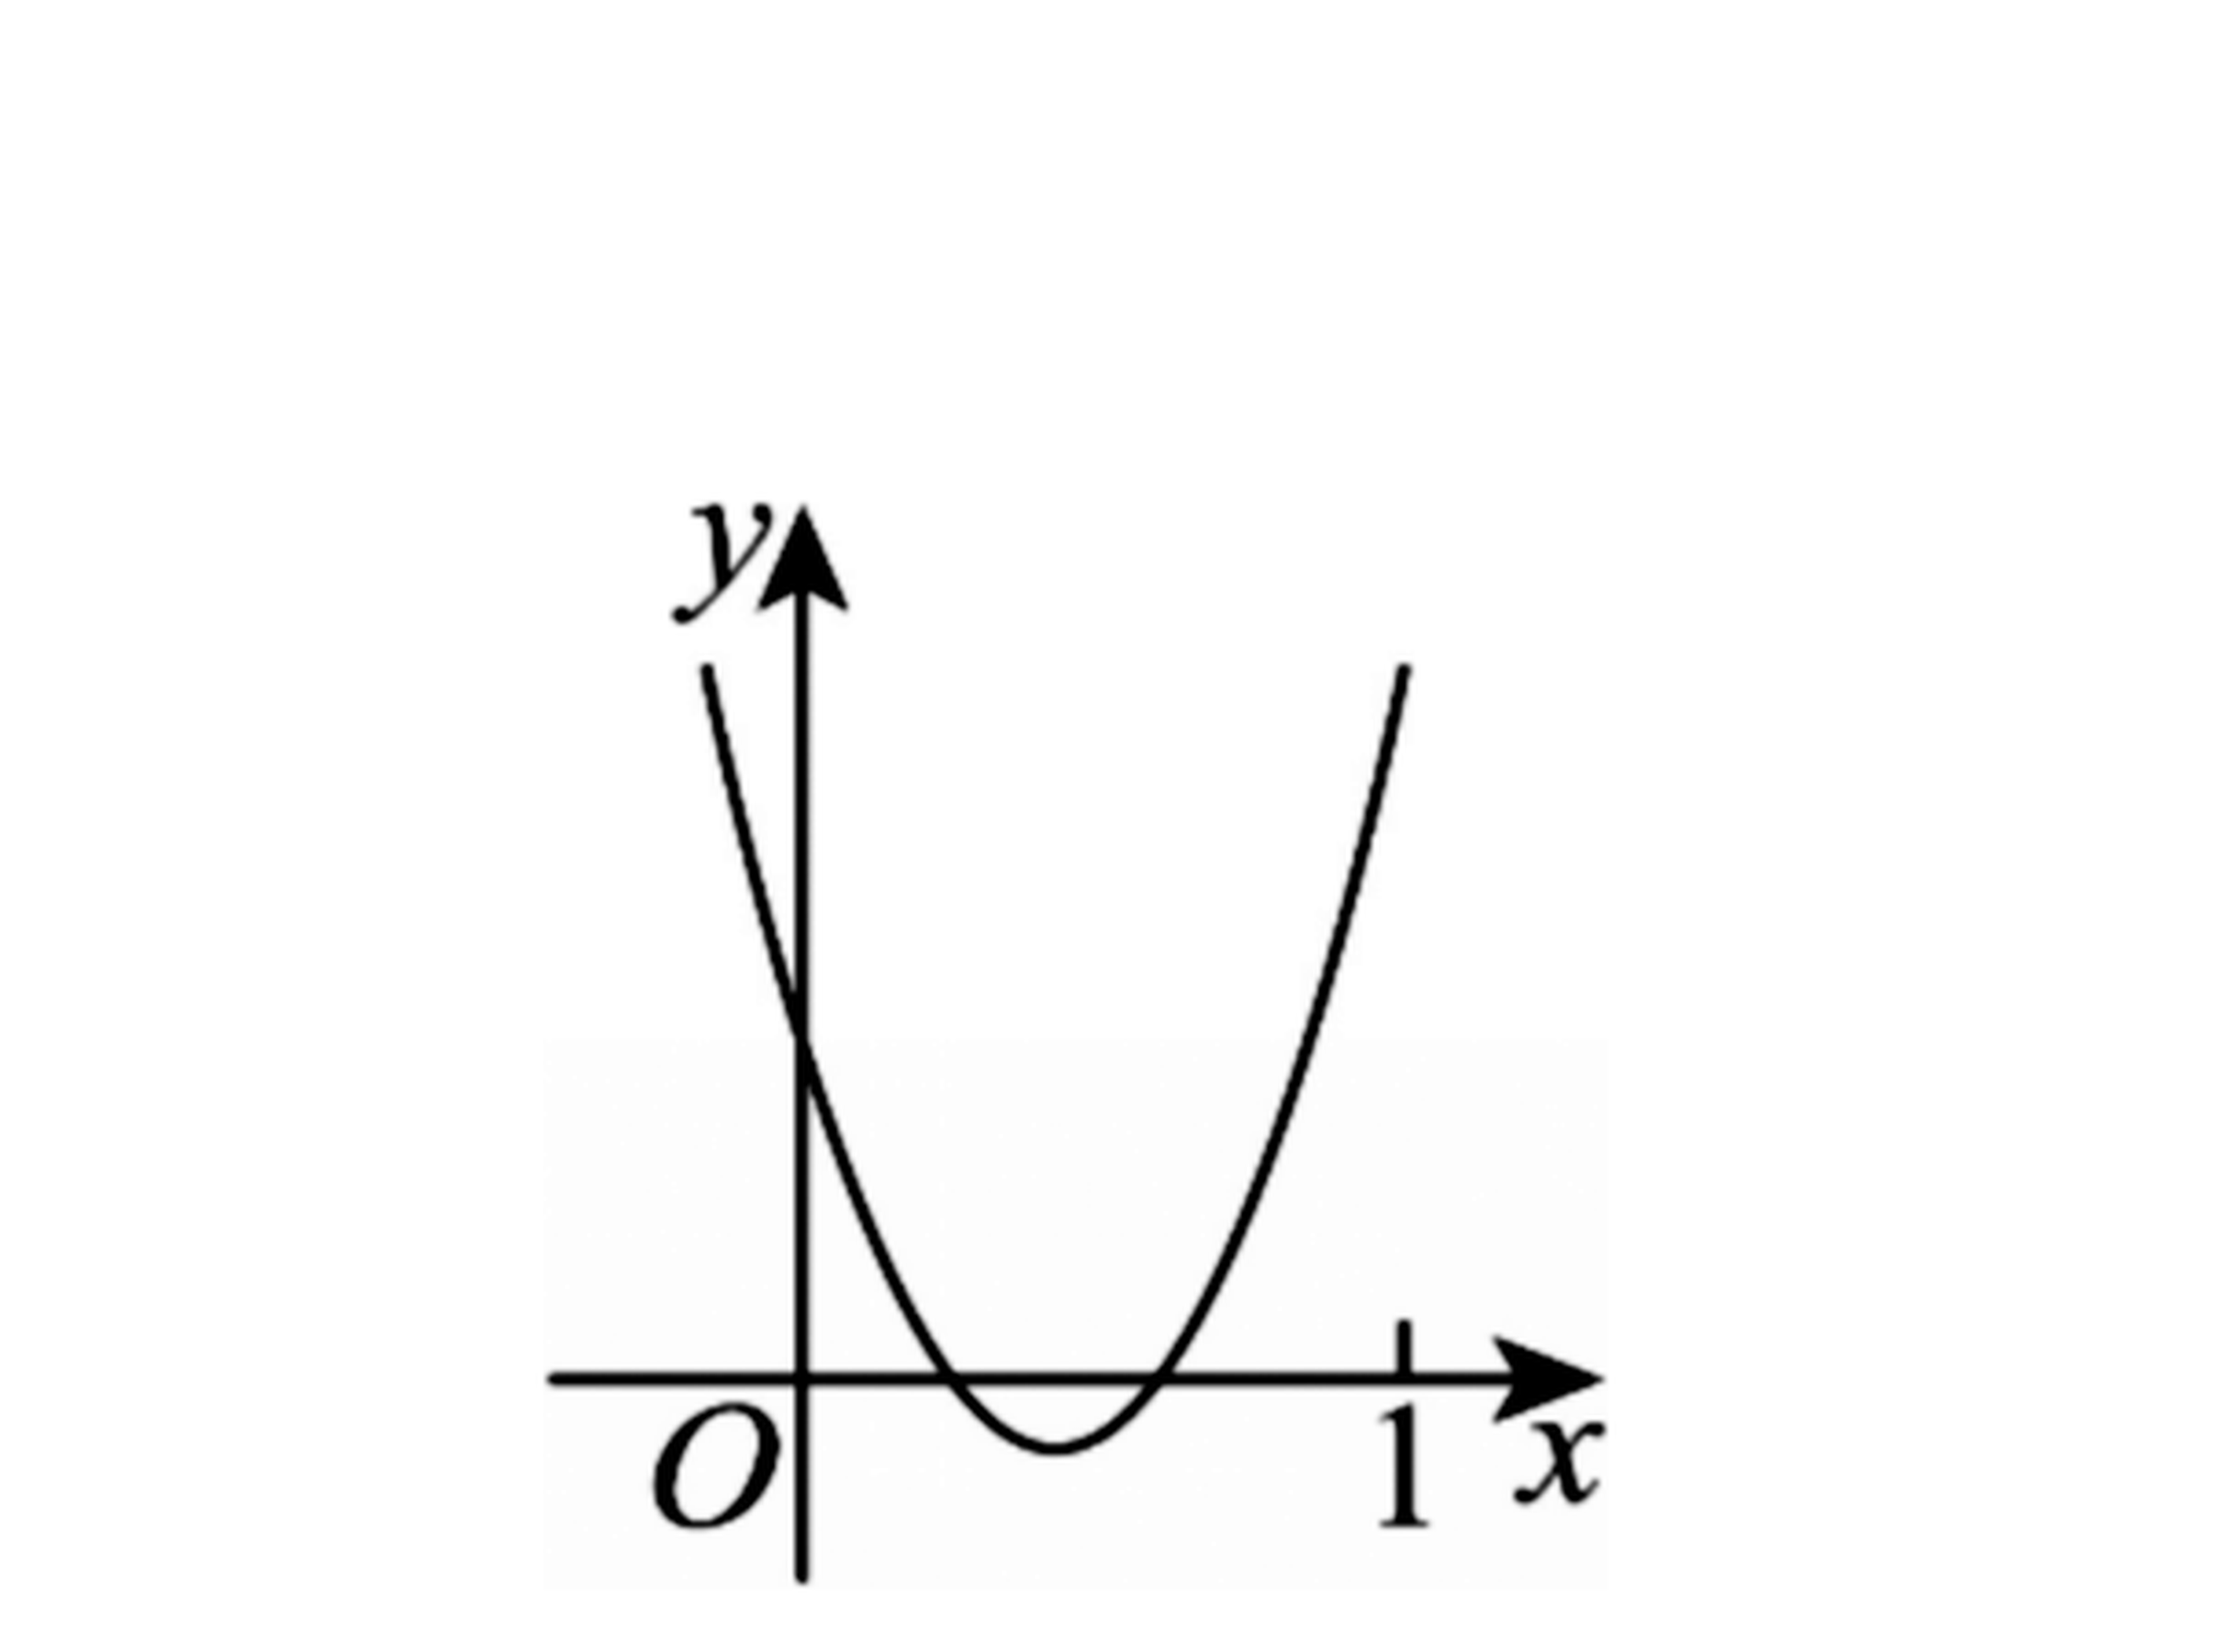
\includegraphics[width=0.32\textwidth]{figures/gao154_q15_stem.png}
\end{center}

\keepwithprev
\begin{center}
% 四幅指数函数图像选项取 05 页上半，按原卷 2×2 排布合并为一张，去粉色水印、去色、4× LANCZOS 放大；三版都出
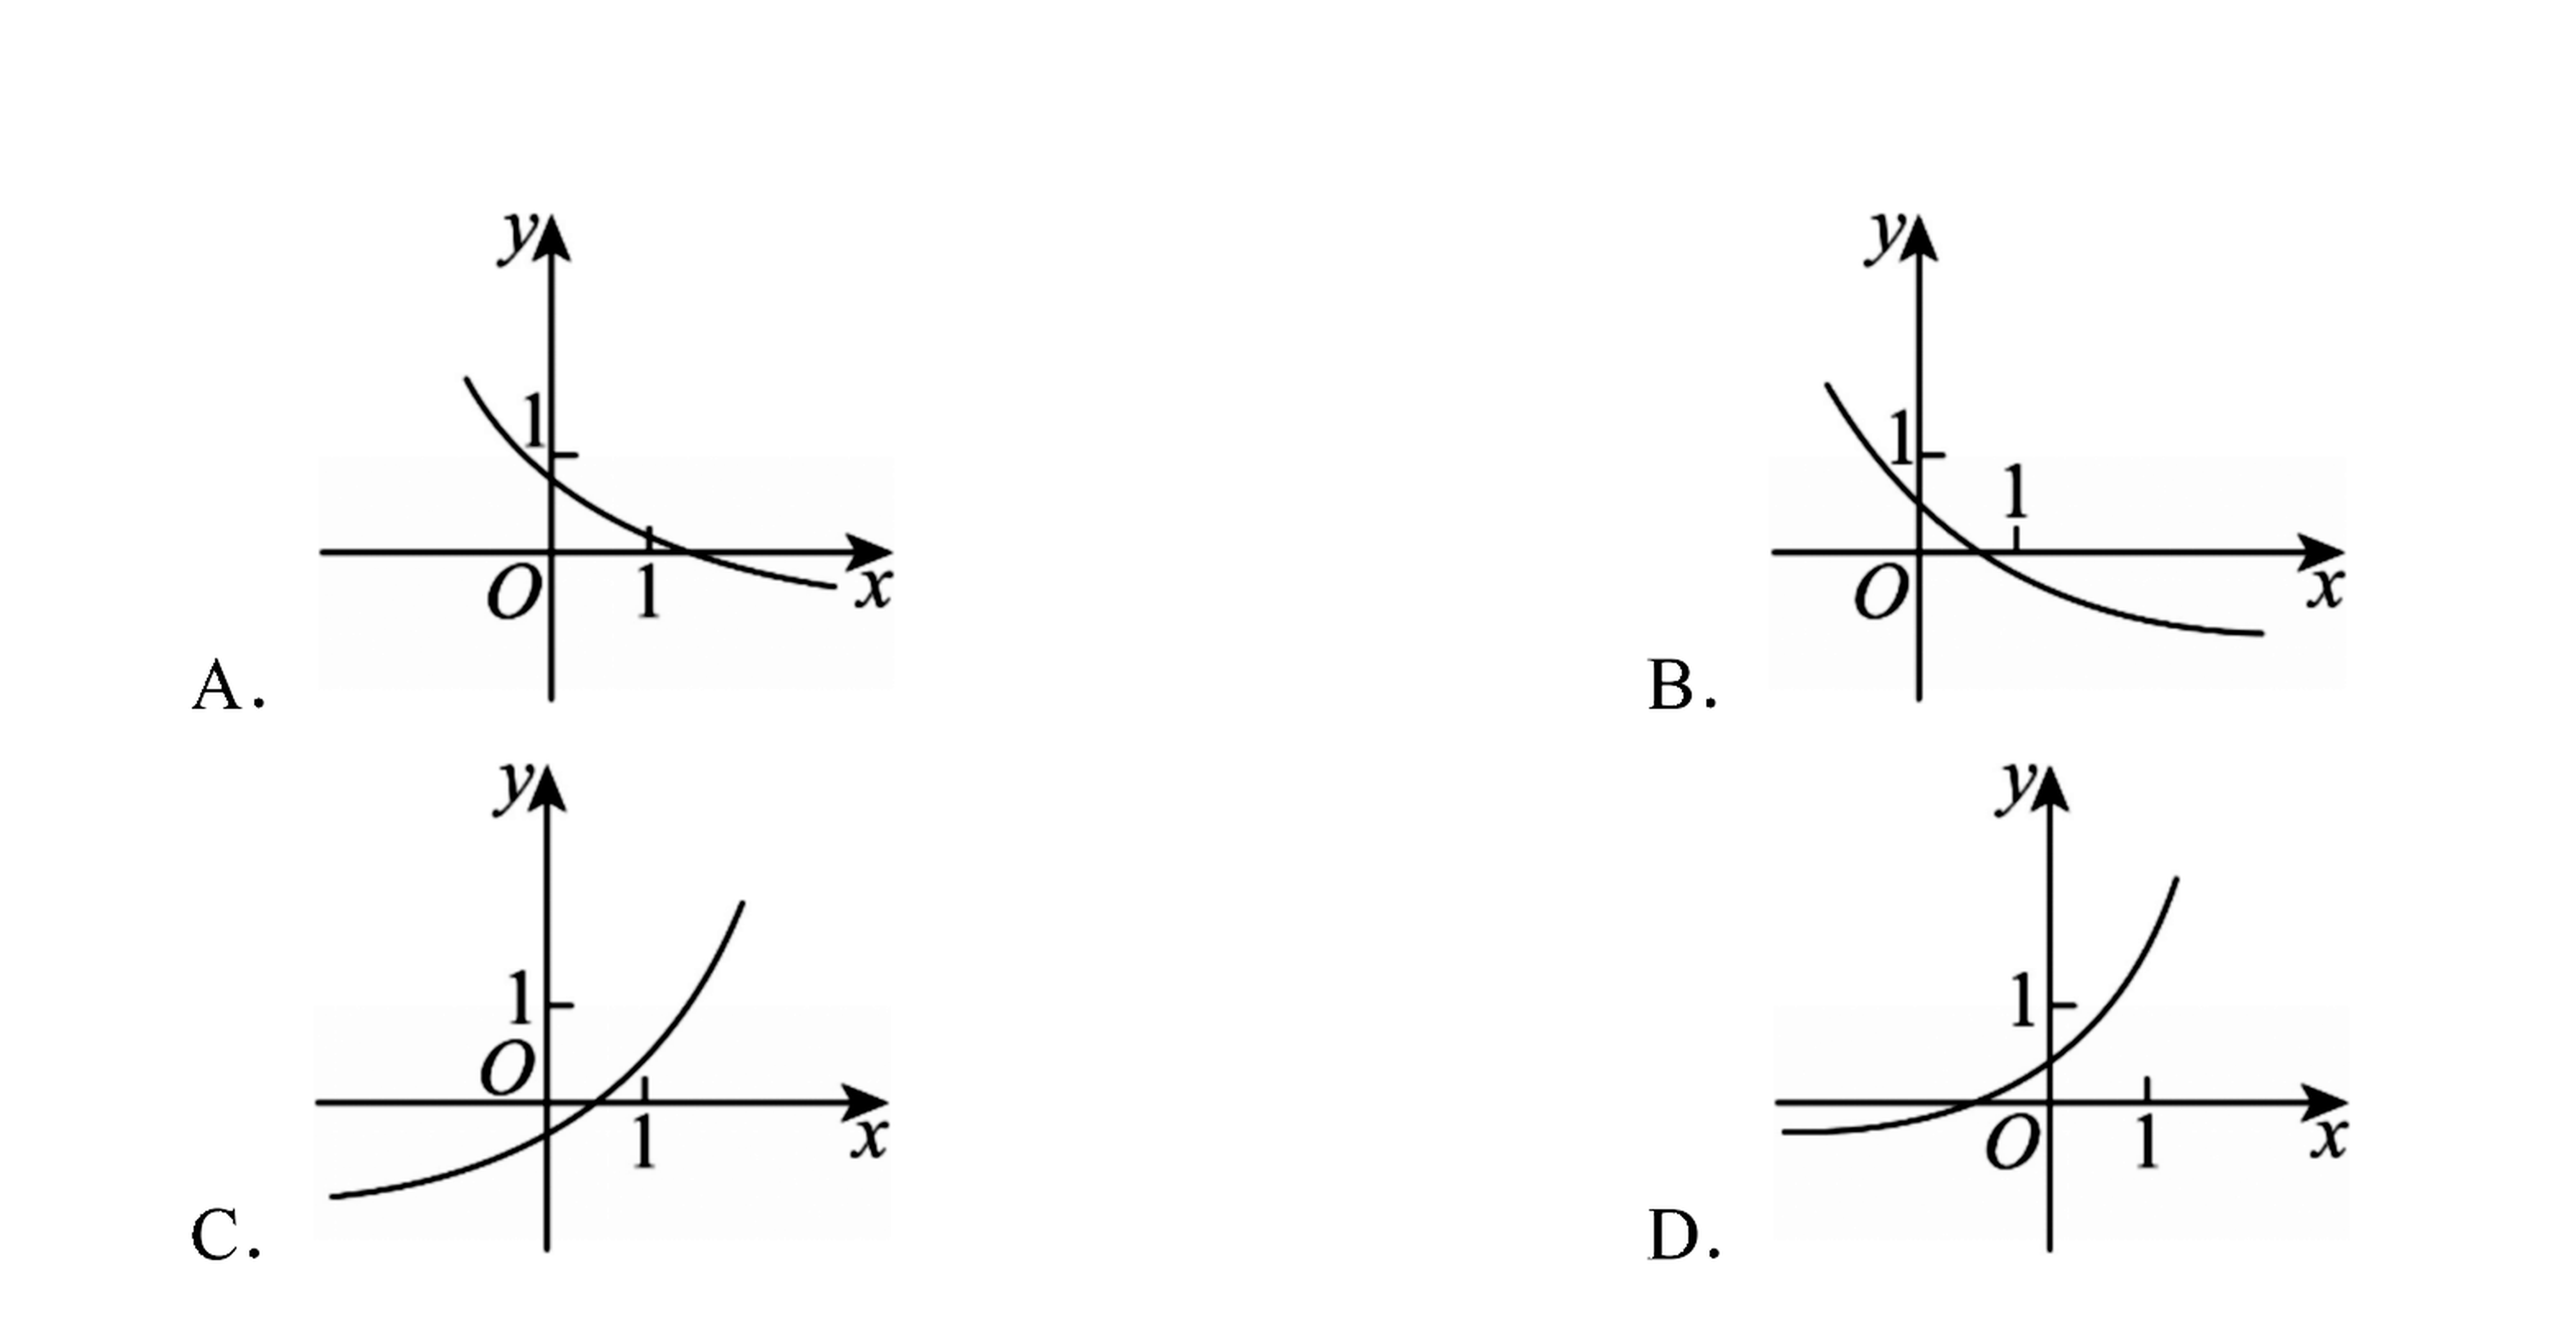
\includegraphics[width=0.80\textwidth]{figures/gao154_q15_opts.png}
\end{center}

\ifanswer
\solbegin
\step{由题意得 $0<a<b<1$，所以 $g(x)=a^x-b$ 在定义域 $\R$ 上严格减.}
\step{$g(0)=a^0-b=1-b>0$，$g(1)=a^1-b=a-b<0$，故 B 符合题意.}
\step{故选 $B$.}
\solend
\fi

% === Q16 === 高斯取整；解析 13 行，故选 C
\item 设 $[a]$ 表示不超过 $a$ 的最大整数，如 $[1.2]=1$，$[-3.2]=-4$，若 $x$、$y$、$z$ 为正实数，则 $\left[\dfrac{y+z}{x}\right]+\left[\dfrac{z+x}{y}\right]+\left[\dfrac{x+y}{z}\right]$ 的最小值为\mbox{（\quad）}

\keepwithprev
A. 2\qquad\qquad B. 3\qquad\qquad C. 4\qquad\qquad D. 6

\ifanswer
\solbegin
\step{若 $x$、$y$、$z$ 为正实数，}
\step{结合基本不等式得 $\dfrac{y+z}{x}+\dfrac{z+x}{y}+\dfrac{x+y}{z}=\dfrac yx+\dfrac xy+\dfrac zx+\dfrac xz+\dfrac zy+\dfrac yz$}
\step{$\geqslant2\sqrt{\dfrac yx\cdot\dfrac xy}+2\sqrt{\dfrac zx\cdot\dfrac xz}+2\sqrt{\dfrac zy\cdot\dfrac yz}=6$，当且仅当 $x=y=z$ 时取等号，}
\step{即 $\dfrac{y+z}{x}$，$\dfrac{z+x}{y}$，$\dfrac{x+y}{z}$ 中至少有一个不小于 2，不妨设 $\dfrac{y+z}{x}\geqslant\dfrac{z+x}{y}\geqslant\dfrac{x+y}{z}$，}
\step{$[a]$ 表示不超过 $a$ 的最大整数和 $\dfrac{y+z}{x}$，$\dfrac{z+x}{y}$，$\dfrac{x+y}{z}$ 中至少有一个不小于 2，}% 原卷此行把两句连写，照录未改（见 ⑤ 3）
\step{得 $\left[\dfrac{y+z}{x}\right]\geqslant2$，所以 $\left[\dfrac{y+z}{x}\right]+\left[\dfrac{z+x}{y}\right]+\left[\dfrac{x+y}{z}\right]\geqslant2$，}
\step{假设 $\left[\dfrac{y+z}{x}\right]+\left[\dfrac{z+x}{y}\right]+\left[\dfrac{x+y}{z}\right]$ 的最小值为 2，$\left[\dfrac{y+z}{x}\right]=2$，$\left[\dfrac{z+x}{y}\right]+\left[\dfrac{x+y}{z}\right]=0$，}
\step{所以 $2\leqslant\dfrac{y+z}{x}<3$，$0<\dfrac{z+x}{y}<1$，$0<\dfrac{x+y}{z}<1$，所以 $2<\dfrac{y+z}{x}+\dfrac{z+x}{y}+\dfrac{x+y}{z}<5$，}
\step{与 $\dfrac{y+z}{x}+\dfrac{z+x}{y}+\dfrac{x+y}{z}\geqslant6$ 矛盾，假设不成立，A 错误；}
\step{假设 $\left[\dfrac{y+z}{x}\right]+\left[\dfrac{z+x}{y}\right]+\left[\dfrac{x+y}{z}\right]$ 的最小值为 3，}
\step{则 $\left[\dfrac{y+z}{x}\right]=2$，$\left[\dfrac{z+x}{y}\right]=1$，$\left[\dfrac{x+y}{z}\right]=0$ 或 $\left[\dfrac{y+z}{x}\right]=3$，$\left[\dfrac{z+x}{y}\right]=\left[\dfrac{x+y}{z}\right]=0$，}
\step{同理可得 $3<\dfrac{y+z}{x}+\dfrac{z+x}{y}+\dfrac{x+y}{z}<6$，显然不成立，B 错误；}
\step{假设 $\left[\dfrac{y+z}{x}\right]+\left[\dfrac{z+x}{y}\right]+\left[\dfrac{x+y}{z}\right]$ 的最小值为 4，易得 $4<\dfrac{y+z}{x}+\dfrac{z+x}{y}+\dfrac{x+y}{z}<7$，}
\step{若取 $x=100$，$y=103$，$z=104$，则 $\left[\dfrac{y+z}{x}\right]=2$，$\left[\dfrac{z+x}{y}\right]=1$，$\left[\dfrac{x+y}{z}\right]=1$，}
\step{即 $\left[\dfrac{y+z}{x}\right]+\left[\dfrac{z+x}{y}\right]+\left[\dfrac{x+y}{z}\right]=4$，假设成立，C 正确，D 错误.}
\step{故选 $C$.}
\solend
\fi

\end{enumerate}

\bigsec{三、解答题}

\begin{enumerate}
\setcounter{enumi}{16}

% === Q17 === $B\subset A$ 单线照录；cases 块；解析 5 行
\item 设集合 $A=\{x\mid x^2+2x-3<0\}$，集合 $B=\{x\mid\lvert x+a\rvert<1\}$.

(1) 若 $a=3$，求 $A\cup B$；

(2) 设命题 $p:x\in A$，命题 $q:x\in B$，若 $p$ 是 $q$ 成立的必要不充分条件，求实数 $a$ 的取值范围.

\ifanswer
\solbegin
\step{(1) $A=(-3,1)$，}
\step{当 $a=3$ 时，$\lvert x+3\rvert<1$，解得 $-4<x<-2$，所以 $B=(-4,-2)$，}
\step{所以 $A\cup B=(-4,1)$.}
\step{(2) 因为 $p$ 是 $q$ 成立的必要不充分条件，所以 $B\subset A$.}
\step{因为 $A=(-3,1)$，$B=(-a-1,-a+1)$，所以 $\begin{cases}-a-1\geqslant-3\\-a+1<1\end{cases}$ 或 $\begin{cases}-a-1>-3\\-a+1\leqslant1\end{cases}$，解得 $0\leqslant a\leqslant2$.}
\solend
\fi

% === Q18 === 判别式 \Delta 两处照录；解析 9 行
\item 已知关于 $x$ 的一元二次方程 $x^2-mx+4m^2-3=0$ 的两个实根分别为 $x_1,x_2$.

(1) 若 $x_1,x_2$ 满足 $x_1+x_2=x_1x_2$，求实数 $m$ 的值；

(2) 求 $x_1^2+x_2^2$ 的最小值.

\ifanswer
\solbegin
\step{(1) 由韦达定理 $x_1+x_2=m$，$x_1x_2=4m^2-3$，}
\step{$\Delta=m^2-4(4m^2-3)=-15m^2+12\geqslant0$，即 $m^2\leqslant\dfrac45$.}
\step{由 $x_1+x_2=x_1x_2$ 得 $m=4m^2-3$，即 $4m^2-m-3=0$，}
\step{解得 $m=1$ 或 $m=-\dfrac34$.}
\step{$m=1$ 时 $m^2=1>\dfrac45$，$\Delta<0$，舍去；}
\step{$m=-\dfrac34$ 时 $m^2=\dfrac9{16}<\dfrac45$，符合，故 $m=-\dfrac34$.}
\step{(2) $x_1^2+x_2^2=(x_1+x_2)^2-2x_1x_2=m^2-2(4m^2-3)=-7m^2+6$，}
\step{函数 $y=-7m^2+6$ 开口向下，对称轴为 $m=0$，}% 原卷此处称求「最小值」，实为闭区间 $m^2\le\frac45$ 上的最小值，照录未改（见 ⑤ 4）
\step{故 $y_{\min}=-7\cdot\dfrac45+6=-\dfrac{28}{5}+\dfrac{30}{5}=\dfrac25$.}
\solend
\fi

% === Q19 === 全称命题；cases 块；解析 9 行
\item 设命题 $p$：对任意 $x\in\R$，不等式 $2mx^2+2mx+1>0$ 恒成立，$q:m\in\{m\mid\log_2(m-1)<1\}$.

(1) 若 $p$ 为真命题，求实数 $m$ 的取值范围；

(2) 若命题 $p$、$q$ 有且只有一个是真命题，求实数 $m$ 的取值范围.

\ifanswer
\solbegin
\step{(1) 由 $p$ 为真命题，得 $\forall x\in\R$，不等式 $2mx^2+2mx+1>0$ 恒成立，}
\step{当 $m=0$ 时，$1>0$ 恒成立；}
\step{当 $m\ne0$ 时，$\begin{cases}2m>0\\\Delta=4m^2-8m<0\end{cases}$，解得 $0<m<2$；}
\step{综上，$0\leqslant m<2$，即 $m$ 的取值范围是 $[0,2)$；}
\step{(2) 若 $q$ 为真，则有 $\log_2(m-1)<1$，得 $0<m-1<2$，解得 $1<m<3$，}
\step{因此命题 $q:m\in\{m\mid1<m<3\}$，由 (1) 得命题 $p:\{m\mid0\leqslant m<2\}$，}
\step{而命题 $p$、$q$ 有且只有一个是真命题，}
\step{当 $p$ 真 $q$ 假时，$\begin{cases}0\leqslant m<2\\m\leqslant1\text{ 或 }m\geqslant3\end{cases}$，解得 $0\leqslant m\leqslant1$，}
\step{当 $p$ 假 $q$ 真时，$\begin{cases}m<0\text{ 或 }m\geqslant2\\1<m<3\end{cases}$，解得 $2\leqslant m<3$，}
\step{故实数 $m$ 的取值范围是 $\{m\mid0\leqslant m\leqslant1\text{ 或 }2\leqslant m<3\}$.}
\solend
\fi

% === Q20 === Labubu 成本题；解析 10 行
\item Labubu 公司拟在 2027 年初推出智能机器人系列玩偶（单位：套）. 根据以往经验，其中一条生产线每月生产 $x$ 套玩具的成本 $P$ 由两部分费用（单位：元）构成：

(i) 固定成本（与生产玩具套数 $x$ 无关），总计 160000 元；

(ii) 每生产 $x$ 套需另投入的生产成本 $c(x)$ 元，其中 $c(x)=10x+\dfrac1{100}x^2$.

(1) 假设该生产线每月生产出的玩具能全部售出，问：该生产线每月生产玩具多少套时，可使得平均每套所需成本费用最少？此时每套玩具的成本费用是多少？

(2) 假设该生产线每月生产出的玩具能全部售出，但随着 $x$ 的增大，每月生产所需的直接总成本在急剧增加，因此售价也需随着 $x$ 的增大而适当增加. 设每套玩具的售价为 $q(x)$ 元，$q(x)=a+\dfrac xb$（$a,b\in\R$）. 若当月产量为 10000 套时利润最大，此时每套售价为 150 元，试求 $a,b$ 的值.（利润=销售收入$-$成本费用）

\ifanswer
\solbegin
\step{(1) 每月总成本 $P=160000+10x+\dfrac1{100}x^2$，}
\step{平均每套成本为 $\dfrac Px=\dfrac{160000}{x}+10+\dfrac x{100}\geqslant10+2\sqrt{\dfrac{160000}{x}\cdot\dfrac x{100}}=90$.}
\step{等号成立当且仅当 $\dfrac{160000}{x}=\dfrac x{100}$ 时，即 $x=4000$ 时取等号，}
\step{所以每月生产 4000 套时平均每套成本最少，此时每套成本为 90 元.}
\step{(2) 利润 $W(x)=x\cdot q(x)-P=\left(\dfrac1b-\dfrac1{100}\right)x^2+(a-10)x-160000$.}
\step{要在 $x=10000$ 处取得最大值，需 $\dfrac1b-\dfrac1{100}<0$，且对称轴为 $x=10000$，}
\step{故 $-\dfrac{a-10}{2\left(\frac1b-\frac1{100}\right)}=10000$，即 $a-10=-20000\left(\dfrac1b-\dfrac1{100}\right)$.}
\step{又 $q(10000)=a+\dfrac{10000}{b}=150$.}
\step{令 $t=\dfrac1b$，则 $a=150-10000t$，}
\step{代入上式 $140-10000t=-20000t+200$，解得 $t=\dfrac3{500}$，即 $b=\dfrac{500}{3}$；}
\step{再由 $a=150-10000\times\dfrac3{500}=150-60=90$，所以 $a=90$，$b=\dfrac{500}{3}$.}
\solend
\fi

% === Q21 === $A^+$／$A^-$ 新定义；$A\subseteq$ 带下划线照录、\varnothing；解析 16 行
\item 设集合 $A$ 为非空数集，定义 $A^+=\{x\mid x=a+b,a,b\in A\}$，$A^-=\{x\mid x=\lvert a-b\rvert,a,b\in A\}$.

(1) 若集合 $A=\{-1,1\}$，写出集合 $A^+$ 及 $A^-$；

(2) 若集合 $A=\{x_1,x_2,x_3,x_4\}$，$x_1<x_2<x_3<x_4$，且 $A^-=A$，求证：$x_1+x_4=x_2+x_3$；

(3) 若集合 $A\subseteq\{x\mid0\leqslant x\leqslant2020,x\in\N\}$，且 $A^+\cap A^-=\varnothing$，求集合 $A$ 元素的个数的最大值.

\ifanswer
\solbegin
\step{(1) 由 $A=\{-1,1\}$，得 $A^+=\{-2,0,2\}$，$A^-=\{0,2\}$；}
\step{(2) 由于集合 $A=\{x_1,x_2,x_3,x_4\}$，$x_1<x_2<x_3<x_4$，且 $A^-=A$，}
\step{所以 $A^-$ 中也只包含四个元素，即 $A^-=\{0,x_2-x_1,x_3-x_1,x_4-x_1\}$，}
\step{剩下的 $x_3-x_2=x_4-x_3=x_2-x_1$，所以 $x_1+x_4=x_2+x_3$；}
\step{(3) 设 $A=\{a_1,a_2,\cdots,a_k\}$ 满足题意，其中 $a_1<a_2<\cdots<a_k$，}
\step{则 $2a_1<a_1+a_2<a_1+a_3<\cdots<a_1+a_k<a_2+a_k<a_3+a_k<\cdots<a_{k-1}+a_k<2a_k$，所以 $\lvert A^+\rvert\geqslant2k-1$，}
\step{且 $a_1-a_1<a_2-a_1<a_3-a_1<\cdots<a_k-a_1$，所以 $\lvert A^-\rvert\geqslant k$，}
\step{因为 $A^+\cap A^-=\varnothing$，所以 $\lvert A^+\cup A^-\rvert=\lvert A^+\rvert+\lvert A^-\rvert\geqslant3k-1$，}
\step{$A^+\cup A^-$ 中最小的元素为 0，最大的元素为 $2a_k$，所以 $\lvert A^+\cup A^-\rvert\leqslant2a_k+1$，}
\step{所以 $3k-1\leqslant2a_k+1\leqslant4041$（$k\in\N^*$），所以 $k\leqslant1347$，}
\step{实际上当 $A=\{674,675,676,\cdots,2020\}$ 时满足题意，证明如下：}
\step{设 $A=\{m,m+1,m+2,\cdots,2020\}$，$m\in\N$，}
\step{则 $A^+=\{2m,2m+1,2m+2,\cdots,4040\}$，$A^-=\{0,1,2,\cdots,2020-m\}$，}
\step{由题意得 $2020-m<2m$，即 $m>673\dfrac13$，}
\step{故 $m$ 的最小值为 674，于是当 $m=674$ 时，$A$ 中元素最多，}
\step{即 $A=\{674,675,676,\cdots,2020\}$ 时满足题意，}
\step{综上所述，集合 $A$ 中元素的个数的最大值是 1347.}
\solend
\fi

\end{enumerate}

\bigsec{附加题}

\begin{enumerate}

% === 附加题 1 === 另起编号 1；「n 元集和集」弯引号；解析 6 行
\item 设集合 $A=\{a_1,a_2,a_3,a_4\}$，$C=\{2,3,4,6\}$，新定义：集合 $A$ 中所有含 $n$ 个元素的子集中 $n$ 个元素之和的不同值组成的集合为“$n$ 元集和集”. 若 $A$ 的“3 元集和集”为 $C$，则集合 $A=$\blankline[4.4em].

\ifanswer
\solbegin
\step{集合 $A$ 的 3 元子集共有 4 个：$\{a_1,a_2,a_3\}$，$\{a_1,a_2,a_4\}$，$\{a_1,a_3,a_4\}$，$\{a_2,a_3,a_4\}$，}
\step{集合 $C=\{a_1+a_2+a_3,a_1+a_2+a_4,a_1+a_3+a_4,a_2+a_3+a_4\}$，}
\step{不妨令 $a_1<a_2<a_3<a_4$，}
\step{则 $a_1+a_2+a_3<a_1+a_2+a_4<a_1+a_3+a_4<a_2+a_3+a_4$，}
\step{而 $C=\{2,3,4,6\}$，因此 $\begin{cases}a_1+a_2+a_3=2\\a_1+a_2+a_4=3\\a_1+a_3+a_4=4\\a_2+a_3+a_4=6\end{cases}$，相加化简得 $a_1+a_2+a_3+a_4=5$，}
\step{解得 $a_1=-1$，$a_2=1$，$a_3=2$，$a_4=3$，所以 $A=\{-1,1,2,3\}$.}
\solend
\fi

% === 附加题 2 === 解析配图（仅答案版出）；四选项；解析 15 行，故选 A
\item 已知函数 $f(x)=\log_p x+q$，其中 $p>0$ 且 $p\ne1$，曲线 $y=f(x)$ 经过 $P(1,2)$、$Q(2,3)$ 两点. 设 $g(x)=f(x)\cdot[f(x)-2]$，若 $\lvert g(a)\rvert=\lvert g(b)\rvert=\lvert g(c)\rvert=\lvert g(d)\rvert$，且 $a<b<c<d$，则 $ad(b+c)$ 的取值范围为\mbox{（\quad）}

\keepwithprev
A. $\left(\dfrac14,\dfrac5{16}\right)$\qquad B. $\left(\dfrac18,\dfrac5{16}\right)$\qquad C. $\left(\dfrac14,\dfrac25\right)$\qquad D. $\left(\dfrac18,\dfrac25\right)$

\ifanswer
\solbegin
\step{函数 $f(x)=\log_p x+q$，且曲线 $y=f(x)$ 经过点 $P(1,2)$ 和 $Q(2,3)$，}
\step{所以 $\begin{cases}f(1)=q=2\\f(2)=\log_p2+q=3\end{cases}$，解得 $p=2$，$q=2$，$f(x)=\log_2 x+2$.}
\step{不妨设 $\lvert g(x)\rvert=k$，令 $\log_2 x=m$，则 $f(x)\cdot[f(x)-2]=m(m+2)=m^2+2m$，}
\step{画出函数 $y=\lvert m^2+2m\rvert$ 的图象，如图所示，}
\begin{center}
% $y=|m(m+2)|$ 图像取 11 页右上，去粉色水印、去色、4× LANCZOS 放大；仅答案版出
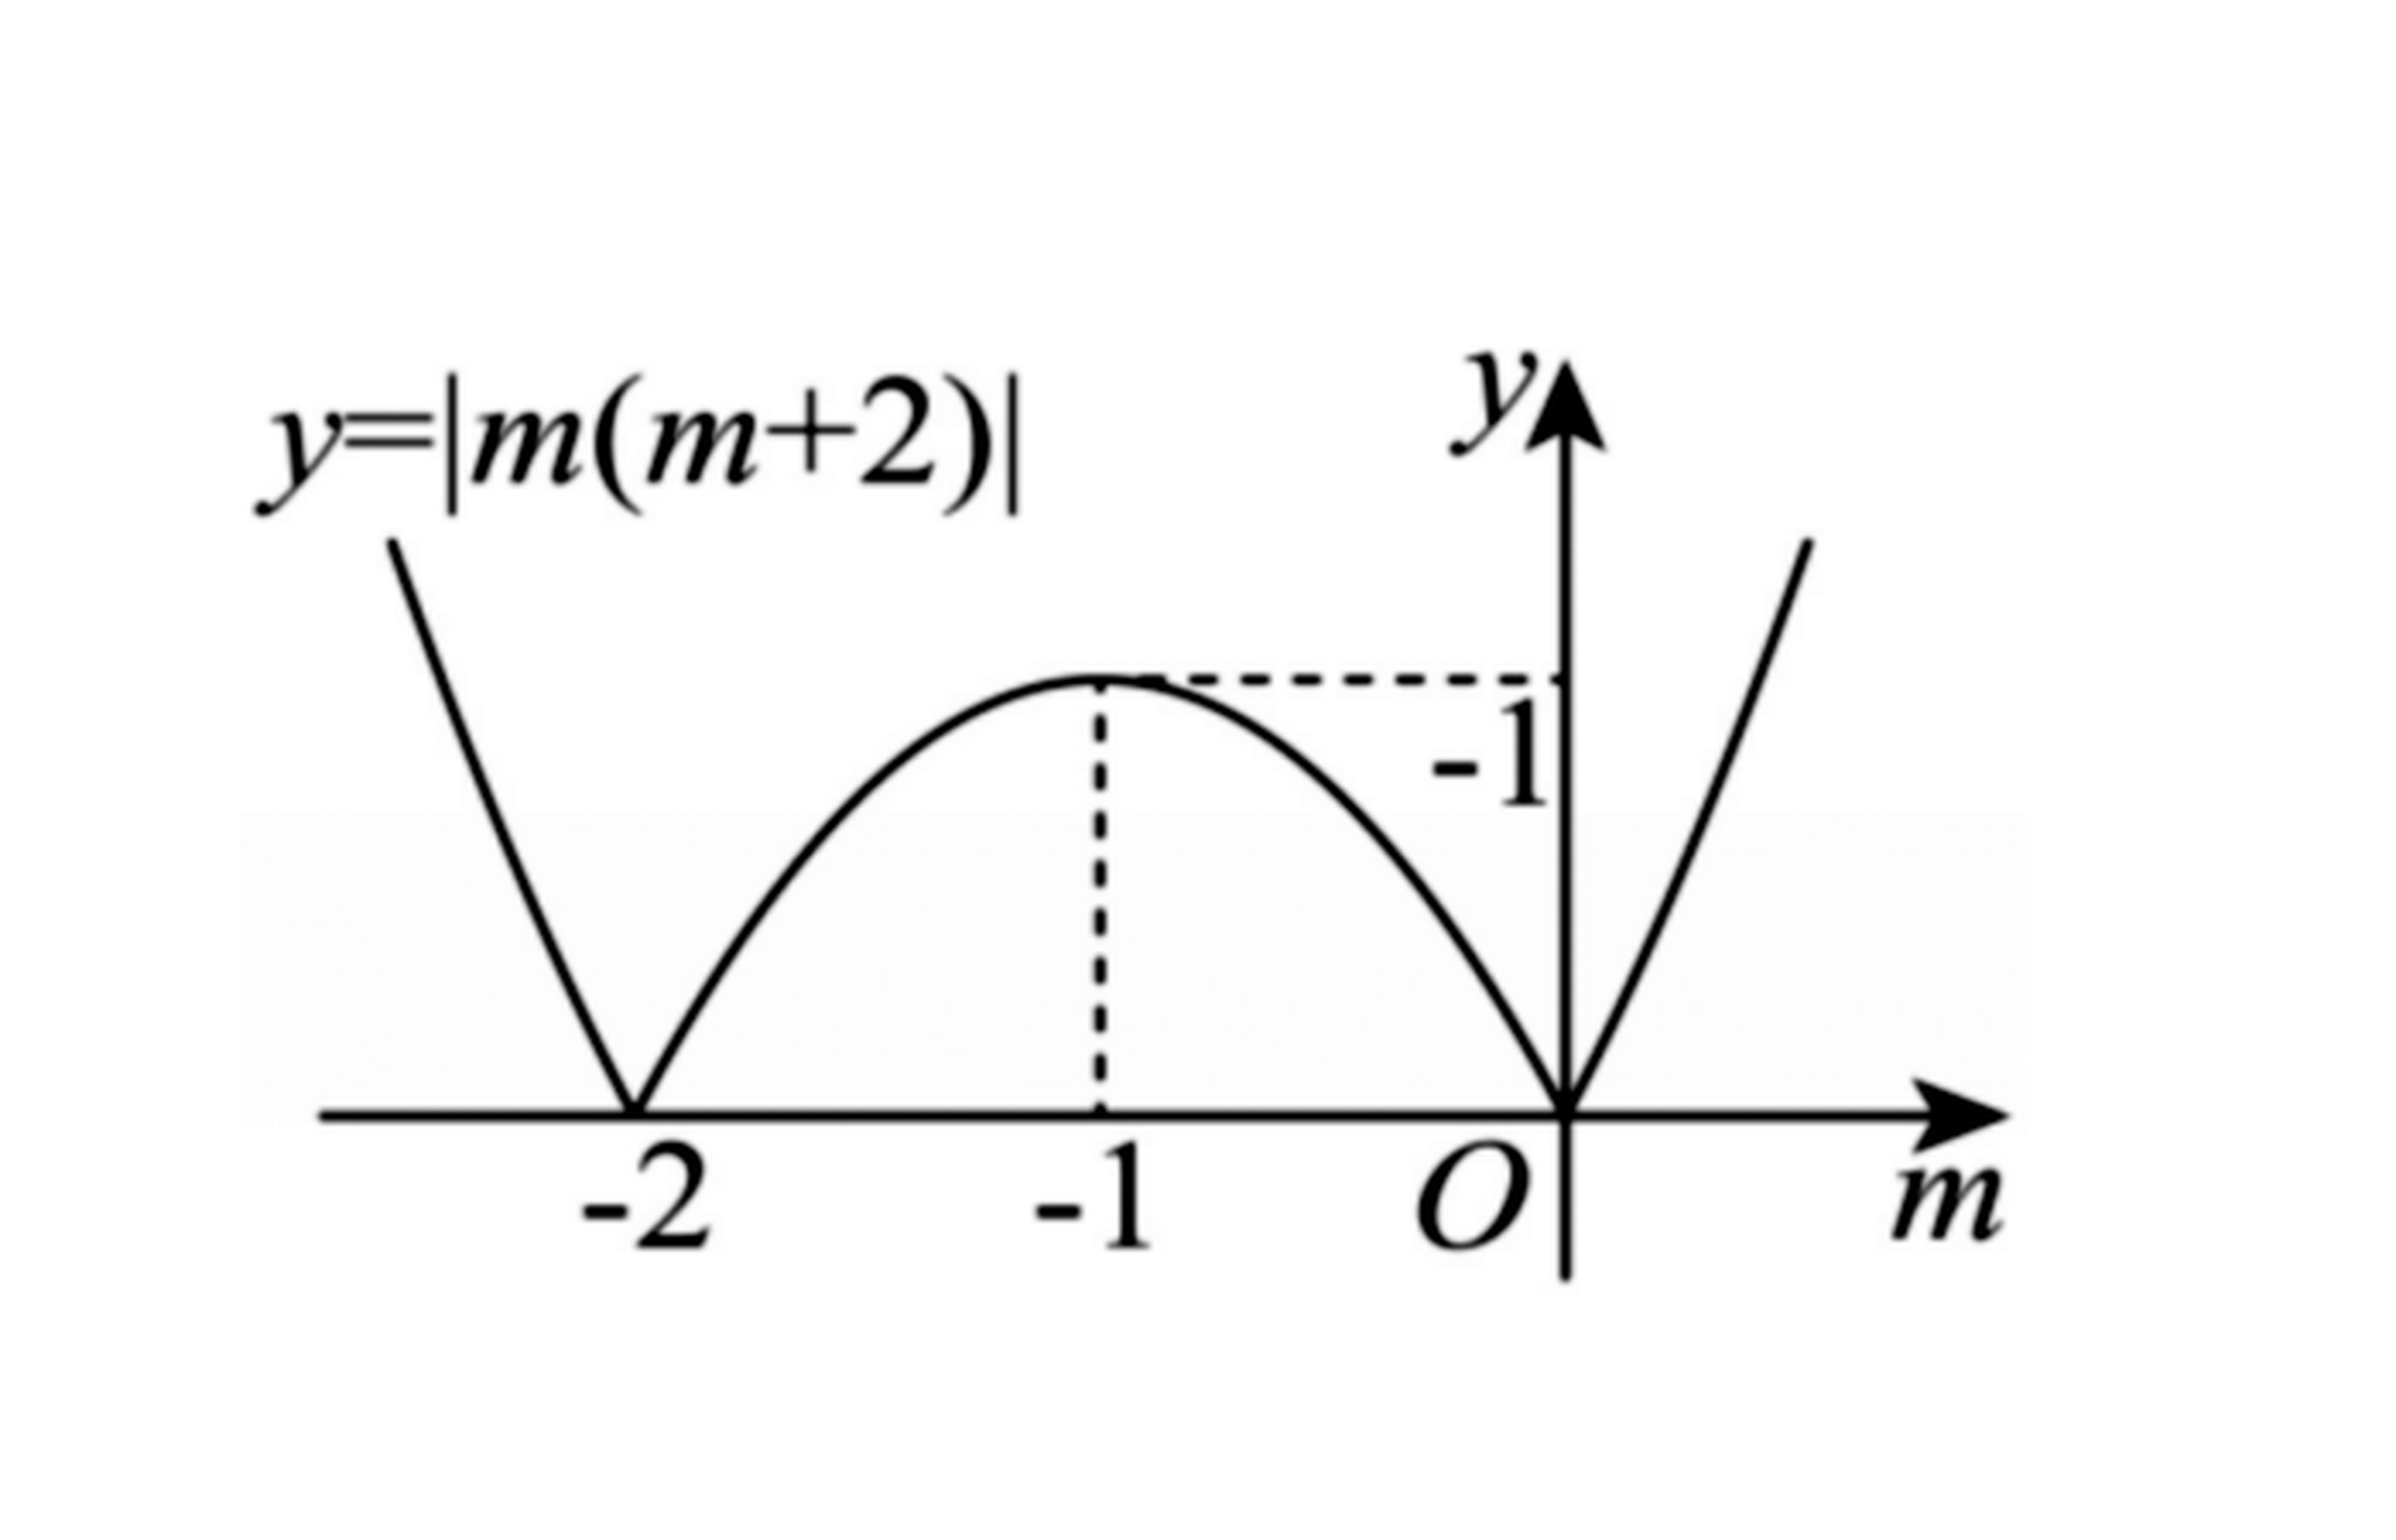
\includegraphics[width=0.46\textwidth]{figures/gao154_fujia2.png}
\end{center}
\step{由图像得 $k\in(0,1)$，}
\step{所以方程 $m^2+2m=k$ 和 $m^2+2m=-k$ 各有两个不同的根，}
\step{其中方程 $m^2+2m-k=0$ 的两根为 $m=-1\pm\sqrt{1+k}$，}
\step{方程 $m^2+2m+k=0$ 的两根为 $m=-1\pm\sqrt{1-k}$，}
\step{所以 $m_1=-1-\sqrt{1+k}$，$m_2=-1-\sqrt{1-k}$，$m_3=-1+\sqrt{1-k}$，$m_4=-1+\sqrt{1+k}$，且 $m_1<m_2<m_3<m_4$，}
\step{由 $m=\log_2 x$，则 $x=2^m$，}
\step{所以 $a=2^{-1-\sqrt{1+k}}$，$b=2^{-1-\sqrt{1-k}}$，$c=2^{-1+\sqrt{1-k}}$，$d=2^{-1+\sqrt{1+k}}$，}
\step{所以 $ad=2^{-1-\sqrt{1+k}}\times2^{-1+\sqrt{1+k}}=2^{(-1-\sqrt{1+k})+(-1+\sqrt{1+k})}=2^{-2}=\dfrac14$，}
\step{$b+c=2^{-1-\sqrt{1-k}}+2^{-1+\sqrt{1-k}}=\dfrac{2^{-\sqrt{1-k}}+2^{\sqrt{1-k}}}{2}$，}
\step{令 $s=\sqrt{1-k}$，其中 $s\in(0,1)$，则 $b+c=\dfrac12\left(2^{-s}+2^s\right)$，}
\step{设函数 $y=2^s+\dfrac1{2^s}$，令 $r=2^s\in(1,2)$，所以 $y=r+\dfrac1r$ 在 $(1,2)$ 上严格增，}
\step{所以函数 $y=2^s+\dfrac1{2^s}$ 在 $(0,1)$ 上严格增，所以 $y=2^s+\dfrac1{2^s}\in\left(2,\dfrac52\right)$，}
\step{所以 $b+c=\dfrac{2^{-s}+2^s}{2}\in\left(1,\dfrac54\right)$，$ad(b+c)=\dfrac{b+c}{4}\in\left(\dfrac14,\dfrac5{16}\right)$，}
\step{所以 $ad(b+c)$ 的取值范围是 $\left(\dfrac14,\dfrac5{16}\right)$，故选 $A$.}
\solend
\fi

\end{enumerate}

\end{document}
"
% 紧凑版：xelatex "\def\iscompact{1}% 高一154_徐汇中学_期中.tex
%   —— 高一上数学"2026-2027 年徐汇中学高一上期中"（试卷版/答案版/紧凑版）
% 试卷版：xelatex 高一154_徐汇中学_期中.tex
% 答案版：xelatex "\def\isanswer{1}\input{高一154_徐汇中学_期中.tex}"
% 紧凑版：xelatex "\def\iscompact{1}\input{高一154_徐汇中学_期中.tex}"
%
% ① 原始材料：微信公众号"魔都数学加油站"文章，连载"27学年高一154"，原文标题
% "27学年高一154——2026-2027年上海市徐汇中学高一上期中"；
% 原文链接：https://mp.weixin.qq.com/s/Qs2T7Zwsug-KKFE2wefDUg 。
% 正文为 12 张 PNG 页（01/03/04/05/07/11/12 为 2560×3620，
% 02/06/08/09/10 为 4762×6735，同一篇各页分辨率混排，逐页按各自分辨率裁图核对）。
% 体例：讲评版——一、填空题 3—12（10 题）、二、选择题 13—16（4 题）、
% 三、解答题 17—21（5 题）、附加题 1—2（2 题，原卷**另起编号**"1." "2."，
% 不与正题连号，同 高一a 成例），共 21 题；全卷每题均印【解析】
% （逐题核实，见 ② ②）。题目、答案、解析均据原图转录；卷面粉红色水印
% "魔都数学加油站"及公众号页脚未录入。
% 全卷插图清单（逐页通读 12 页确认）：3 组——
%   · Q15 题干配图（$f(x)=(x-a)(x-b)$ 抛物线，04 页右下：x/y 轴、O、1、
%     开口向上两零点均在 (0,1) 内），三版都出，裁 figures/gao154_q15_stem.png；
%   · Q15 四幅图像选项（05 页上半 2×2 排布，A/B/C/D 四幅指数函数图像，
%     合并成一张，照 高一136 Q13/Q22 成例），三版都出，
%     裁 figures/gao154_q15_opts.png；
%   · 附加题第 2 题解析配图（$y=\lvert m(m+2)\rvert$ 图像，11 页右上：
%     W 形折线、$-2$、$-1$、O、虚线 $y=1$ 与 $m=-1$），仅答案版出，
%     裁 figures/gao154_fujia2.png；
%   3 图均取自原卷截图，去粉色水印、去色、4× LANCZOS 放大；Q15 题干图
%   左侧题干残字"的图"已裁白。其余各页逐页确认无其它题目配图、无表格；
%   12 页下半仅水印、无正文。
%
% 卷首标题：原卷印作"2026-2027 年徐汇中学高一上期中"，年份区间按全稿惯例排 en dash；
% 原卷卷面未印副标题，本稿按同期中卷知识模块口径补出"集合与常用逻辑用语、不等式、函数"。
%
% ② 与原卷的排版差异：
%   ① 原文从第 3 题起，本稿保留原题号；共 21 题四节，正题到 21，附加题另起编号
%      1—2（\bigsec{附加题} 后 \begin{enumerate} 不 \setcounter，同 高一a 成例）；
%   ② 全 21 题均印【解析】、用 \solbegin…\solend，无只印【答案】或答案印括号内的题；
%      四道正题选择题答案在解析末句"故选 C／A／B／C"（Q13—Q16）、附加题第 2 题
%      答案在解析末句"故选 A"，括号 \mbox{（\quad）} 留空、不另提 \ans{}；
%      答案版【答案】/【解析】标记数 = 21 = 全卷题数；
%   ③ 原卷卷面未印副标题，本稿按知识模块口径补出；
%   ④ 原卷填空横线按全稿惯例排 \blankline[4.4em]；选择题括号排 \mbox{（\quad）}、
%      四道正题选择题与附加题第 2 题的选项段前按惯例各加 \keepwithprev
%      （Q15 与附加题 2 的选项段是整块图，\keepwithprev 后接 \begin{center}）；
%      解答题不留作答区、不加 \anspace（原卷为讲评版）；
%   ⑤ 数集黑板粗体：Q4"$x,y\in R$"、Q9"$x\in\R$"、Q13 无、
%      Q15"定义域 $\R$"、Q19"$\forall x\in\R$"、Q21"$x\in\N$"与"$k\in\N^*$"、
%      Q20"$a,b\in\R$"、附加题 2 无——原卷印斜体或正体粗体 R/N/N*，
%      按全稿惯例归一 \R／\N／\N^*；绝对值排 \lvert…\rvert
%      （Q5、Q9、Q12、Q13、Q16、Q21、附加题 2），集合描述竖线排 \mid
%      （Q5、Q17、Q19、Q21），不等号按全稿惯例排 \leqslant／\geqslant；
%      空集 \varnothing（Q21 题干 (3)）；
%   ⑥ 子集符号逐处照录、不得统一：Q6 题干印"$\{1,2\}\subset M\subseteq\{1,2,3,4,5\}$"
%      （前单线 ⊂、后带下划线 ⊆，同句两形并用），解析亦两形并用；
%      Q17 解析 (2)"$B\subset A$"印单线 ⊂；Q21 题干 (3)"$A\subseteq\{x\mid\cdots\}$"
%      印带下划线 ⊆——逐处放大核，分别 \subset／\subseteq，照录未统一（见 ④）；
%   ⑦ 判别式 Δ/△：Q18 解析 (1)"$\Delta=m^2-4(4m^2-3)$"与 Q19 解析 (1)
%      "$\Delta=4m^2-8m<0$"两处均印等腰偏高粗三角、照录 \Delta；本卷无扁等边
%      细线 \triangle 用例（见 ④）；
%   ⑧ 中文弯引号照录：Q4"设 $x$、$y\in\R$. 若 $x+y>2$，则 $x>1$ 或 $y>1$"、
%      附加题 1"$n$ 元集和集"与"3 元集和集"；注释里一律 ASCII 引号；
%      数学式内 CJK 用 \text{}（Q5 解集描述"或"、Q19 集合描述的"或"）；
%   ⑨ "图像／图象"逐处放大核：Q15 题干与解析印"图象"（象，无亻）、
%      Q16 无、附加题 2 解析印"图象"与"图像"（"画出函数…的图象"、
%      "由图像得"——两形并用，逐处照录未统一）；Q13/Q14 无数集图像字样；
%      半角逗号在数学组之间是全稿惯例、非笔误，逐处照录（Q3、Q10、Q16、
%      Q18、Q20、Q21 的 $x_1,x_2$ 之类）；行末西文句点 ASCII `.`；
%      行中全角逗号／顿号照录（Q6"3，4，5"、Q20"（单位：元）"、
%      附加题 1"$a_1,a_2,a_3,a_4$"）；
%   ⑩ 复杂式照录别简化：Q3 $a^{\frac{12}{7}}\cdot\left(\frac17\right)^{\frac17}
%      \cdot\sqrt[7]{a^4}$ 与 $7^{-\frac17}a^{\frac{16}{7}}$、Q7 $x^{-m}$、
%      Q8 $\frac{b-2a+2}{2a}$、Q11 $\frac{9+4\sqrt2}{6}$、Q12 $506\frac29$ 与
%      $506\frac49$、Q16 高斯取整 $[a]$、Q20 $c(x)=10x+\frac1{100}x^2$ 与
%      $q(x)=a+\frac xb$、Q21 $A^+$／$A^-$ 与 $|A^+|\geqslant2k-1$、
%      附加题 2 $m=-1\pm\sqrt{1+k}$ 与 $ad(b+c)$；
%      \left…\right 不得拆到不同 $…$ 组（Q5 $\left\{x\mid\cdots\right\}$、
%      Q20 $\left(\frac1b-\frac1{100}\right)$、附加题 2 $\left(\frac14,\frac5{16}\right)$）；
%      cases 块一律 \begin{cases}…\end{cases}；
%   ⑪ 一条 \step = 原卷解析的一个印刷行，cases 块整体算一个印刷行；别并折行、
%      别拆行。Q11 九行、Q12 六行、Q16 十六行、Q20 十一行、Q21 十七行、
%      附加题 2 十八行均按印刷行逐条断，不丢行；
%   ⑫ 配图：Q15 题干小图（三版都出）放 \item 内题干之后 \begin{center}，
%      Q15 四幅选项图（三版都出）放 \keepwithprev 之后的 \begin{center}，
%      Q15 用 \needvspace 守卫把"题干＋两图"整块推走（守卫放 \item 之前，
%      见 高一145 Q14/Q20 与 高一136 Q13 成例）；附加题 2 解析配图（仅答案版出）
%      放 \ifanswer 内 \solbegin…\solend 的 \step 之间（高一73 第 16 题成例）；
%   ⑬ 原卷解析内无红色"法一／法二"之类小标题，故本卷无 \stepm；红色水印
%      "魔都数学加油站"不录入；
%   ⑭ 跨页续印按题合并：见 ⑥；
%
% ③ 行数复核：一条 \step = 原卷解析的一个印刷行，cases 块作一个印刷行计。
%   逐题数（主会话逐页核对定稿）：Q3：1；Q4：1；Q5：3；Q6：4；Q7：3；
%   Q8：1；Q9：5；Q10：4；Q11：9；Q12：6；Q13：5；Q14：4；Q15：3；
%   Q16：16；Q17：5；Q18：9；Q19：10；Q20：11；Q21：17；
%   附加题 1：6；附加题 2：18。
%   合计 141 条 \step（本卷无 \stepm），与原卷逐题印刷行相等。全卷 21 题
%   均设 \solbegin…\solend，答案版【答案】/【解析】标记数 = 21 = 全卷题数。
%
% ④ 判别式／子集符号结论（逐处放大原图照录、不得统一，主会话像素级复核）：
%   判别式：Q18 解析 (1)"$\Delta=m^2-4(4m^2-3)=-15m^2+12\geqslant0$"、
%      Q19 解析 (1)"$\Delta=4m^2-8m<0$"共 2 处，逐处放大确认印等腰偏高
%      粗三角（高>宽、右斜边粗），照录 \Delta；本卷无扁等边细线 \triangle
%      用例，无几何三角形符号。
%   子集：Q6 题干"$\{1,2\}\subset M\subseteq\{1,2,3,4,5\}$"前 ⊂ 单线、
%      后 ⊆ 带下划线（/tmp/gao154/z/zoom/q6_subset.png），解析两处同样两形
%      并用，分别照录 \subset／\subseteq；Q17 解析 (2)"$B\subset A$"单线
%      照录 \subset；Q21 题干 (3)"$A\subseteq\{x\mid\cdots\}$"带下划线
%      照录 \subseteq。本卷 ⊂ 与 ⊆ 混用逐处照录、不得统一。
%      空集 \varnothing（Q21 题干 (3)）、数集 \R／\N／\N^* 归一见 ② ⑤。
%
% ⑤ 存疑照录（放大原图确认，照录未改、正文对应处另有 % 注）：
%   1. Q7 题干印 $f(x)=(3m-1)x^{-m}$，解析首句却写"幂函数 $f(x)=x^\alpha$
%      的系数必须为 1"（用 $\alpha$ 作指数记号），随后 $f(2)=2^\alpha=8$
%      得 $\alpha=3$、$f(x)=x^3$——题干指数 $-m$ 与解析 $\alpha$ 记法不同，
%      系原卷记号前后不一，逐处照录未统一（放大 01/02 页确认）。
%   2. Q11 解析"因为 $u>0,v>0$，由基本不等式得 $\frac{4v}{u}+\frac{2u}{v}
%      \geqslant2\sqrt{\frac{4v}{u}\cdot\frac{2u}{v}}=4\sqrt2$"与
%      "所以 $\frac4u+\frac1v=\frac16\left(\frac4u+\frac1v\right)(2u+v)$"
%      照录，未把 $u,v$ 化简回 $x,y$。
%   3. Q16 解析把"$[a]$ 表示不超过 $a$ 的最大整数"与"和至少有一个不小于 2"
%      连写在同一行（原卷如此），照录未改；末行"假设成立，C 正确，D 错误"照录。
%   4. Q18 解析 (2)"函数 $y=-7m^2+6$ 开口向下，对称轴为 $m=0$"却称求
%      "$y_{\min}$"（实为在 $m^2\leqslant\frac45$ 闭区间上的最小值），
%      照录未改。
%   5. Q20 题干"$q(x)=a+\frac xb$（$a,b\in\R$）"与解析
%      "$W(x)=\left(\frac1b-\frac1{100}\right)x^2+(a-10)x-160000$"照录；
%      末行解得 $a=90,b=\frac{500}{3}$ 照录未化简。
%   6. Q21 题干 (3)"$A\subseteq\{x\mid0\leqslant x\leqslant2020,x\in\N\}$"
%      与解析"$3k-1\leqslant2a_k+1\leqslant4041$（$k\in\N^*$）"照录；
%      末行"集合 $A$ 中元素的个数的最大值是 1347"照录。
%   7. 附加题 1 解析"相加化简得 $a_1+a_2+a_3+a_4=5$"照录；
%      附加题 2 解析"由图像得 $k\in(0,1)$"与"由图像得"／"的图象"两形
%      并用逐处照录（见 ② ⑨）；末行"$ad(b+c)$ 的取值范围是
%      $\left(\frac14,\frac5{16}\right)$，故选 A"照录。
%   全卷除此 7 类外未发现其它笔误／自相矛盾处；21 题均印【解析】、
%   无只印【答案】或答案印括号内的题（见 ② ②）。
%
% ⑥ 跨页续印按题合并说明（逐页核实定稿）：Q3—Q5 题干＋解析在 01 页
%   （Q5 解析末 2 行续 01 页下半）；Q6、Q7 题干＋解析在 01 页下半
%   （Q7 解析余 2 行续 02 页顶）；Q8、Q9 题干＋解析在 02 页上半
%   （Q9 解析余 3 行续 02 页下半）；Q10 题干＋解析在 02 页下半；
%   Q11 题干＋解析前 6 行在 03 页上半、余 3 行续 03 页下半；
%   Q12 题干＋解析前 5 行在 03 页下半、末行续 04 页顶；"二、选择题"
%   标题与 Q13 题干＋选项＋解析在 04 页上半；Q14 题干＋选项＋解析、
%   Q15 题干＋题干配图在 04 页下半；Q15 四幅选项图＋解析、
%   Q16 题干＋选项＋解析首行在 05 页上半，Q16 解析余 12 行在
%   05 页下半—06 页上半；"三、解答题"标题与 Q17 题干＋两问＋解析
%   在 06 页下半；Q18 题干＋两问＋解析在 07 页上半—下半；
%   Q19 题干＋两问＋解析首行在 07 页下半，解析余 8 行在 08 页上半；
%   Q20 题干在 08 页下半，解析 (1) 4 行＋(2) 首 4 行在 08 页下半—09 页上半，
%   (2) 余 2 行在 09 页下半；Q21 题干＋三问＋解析 (1)(2) 4 行在
%   09 页下半—10 页上半，解析 (3) 余 12 行在 10 页上半—下半；
%   "附加题"标题与附加题 1 题干＋解析首 3 行在 10 页下半，
%   余 3 行续 11 页上半；附加题 2 题干＋选项＋解析前 3 行在 11 页上半，
%   解析配图＋余 12 行在 11 页下半—12 页上半，末行
%   "所以 $ad(b+c)$ 的取值范围是 $\left(\frac14,\frac5{16}\right)$，故选 A"
%   为全卷收尾（12 页下半仅水印、无正文）。
%   本稿按题连排，不丢行、不并折行；全卷末题为附加题第 2 题。
%
\documentclass[a4paper,11pt]{article}
\usepackage{common}

\begin{document}

\examtitlest[3]{2026--2027 年徐汇中学高一上期中}{集合与常用逻辑用语、不等式、函数}

\bigsec{一、填空题}

\begin{enumerate}
\setcounter{enumi}{2}

% === Q3 === 分数指数幂照录；解析 1 行
\item 已知 $a>0$，化简 $a^{\frac{12}{7}}\cdot\left(\dfrac17\right)^{\frac17}\cdot\sqrt[7]{a^4}=$\blankline[4.4em].

\ifanswer
\solbegin
\step{$a^{\frac{12}{7}}\cdot\left(\dfrac17\right)^{\frac17}\cdot\sqrt[7]{a^4}=a^{\frac{12}{7}}\cdot(7^{-1})^{\frac17}\cdot a^{\frac47}=7^{-\frac17}a^{\frac{16}{7}}$.}
\solend
\fi

% === Q4 === 反证法；中文弯引号照录；解析 1 行
\item 用反证法证明命题：“设 $x$、$y\in\R$. 若 $x+y>2$，则 $x>1$ 或 $y>1$”时，假设的内容应该是\blankline[4.4em].

\ifanswer
\solbegin
\step{由反证法得，假设的内容应该是 $x\leqslant1$ 且 $y\leqslant1$.}
\solend
\fi

% === Q5 === 分式不等式；cases 块；解析 3 行
\item 不等式 $\dfrac{2x+3}{x-1}\geqslant1$ 的解集为\blankline[4.4em].

\ifanswer
\solbegin
\step{$\dfrac{2x+3}{x-1}\geqslant1$，即 $\dfrac{2x+3}{x-1}-1\geqslant0$，$\dfrac{x+4}{x-1}\geqslant0$，}
\step{等价于 $\begin{cases}(x+4)(x-1)\geqslant0\\x-1\ne0\end{cases}$，解得 $x>1$ 或 $x\leqslant-4$，}
\step{故解集为 $\{x\mid x>1\text{ 或 }x\leqslant-4\}$.}
\solend
\fi

% === Q6 === ⊂ 与 ⊆ 并用照录；解析 4 行
\item 满足条件 $\{1,2\}\subset M\subseteq\{1,2,3,4,5\}$ 的集合 $M$ 的个数为\blankline[4.4em].

\ifanswer
\solbegin
\step{因为 $\{1,2\}\subset M\subseteq\{1,2,3,4,5\}$，所以集合 $M$ 必含有元素 1，2，}
\step{且至少含有元素 3，4，5 中的一个，}
\step{则集合 $M$ 的个数与集合 $\{3,4,5\}$ 的非空子集的个数一样，}
\step{所以集合 $M$ 的个数为 $2^3-1=7$.}
\solend
\fi

% === Q7 === 题干 $x^{-m}$、解析用 $x^\alpha$ 记法，原卷记号差异照录（见 ⑤ 1）；解析 3 行
\item 已知幂函数 $f(x)=(3m-1)x^{-m}$，且 $f(2)=8$，则 $f(m)=$\blankline[4.4em].

\ifanswer
\solbegin
\step{幂函数 $f(x)=x^\alpha$ 的系数必须为 1，所以 $3m-1=1$，得 $m=\dfrac23$.}
\step{又 $f(2)=2^\alpha=8=2^3$，故 $\alpha=3$，即 $f(x)=x^3$，}
\step{所以 $f(m)=f\left(\dfrac23\right)=\left(\dfrac23\right)^3=\dfrac8{27}$.}
\solend
\fi

% === Q8 === 换底公式；解析 1 行
\item 已知 $a=\lg2$，$b=\lg3$，用含 $a,b$ 的代数式表示 $\log_4 75=$\blankline[4.4em].

\ifanswer
\solbegin
\step{$\log_4 75=\dfrac{\lg\left(3\times\frac{10^2}{2^2}\right)}{\lg2^2}=\dfrac{\lg3+2-2\lg2}{2\lg2}=\dfrac{b-2a+2}{2a}$.}
\solend
\fi

% === Q9 === 三角不等式取等；解析 5 行
\item 设 $x\in\R$，则方程 $\lvert x-2\rvert+\lvert3x+1\rvert=\lvert2x+3\rvert$ 的解集是\blankline[4.4em].

\ifanswer
\solbegin
\step{由 $\lvert x-2\rvert=\lvert2-x\rvert$，故原方程可化为 $\lvert2-x\rvert+\lvert3x+1\rvert=\lvert2x+3\rvert$，}
\step{又 $(2-x)+(3x+1)=2x+3$，}
\step{由三角不等式 $\lvert2-x\rvert+\lvert3x+1\rvert\geqslant\lvert(2-x)+(3x+1)\rvert=\lvert2x+3\rvert$，}
\step{当且仅当 $(2-x)(3x+1)\geqslant0$ 等号成立，}
\step{解 $(2-x)(3x+1)\geqslant0$ 得 $-\dfrac13\leqslant x\leqslant2$，故原方程的解集为 $\left[-\dfrac13,2\right]$.}
\solend
\fi

% === Q10 === 韦达定理；cases 块；解析 4 行
\item 已知一元二次不等式 $x^2+bx+c>0$ 的解集为 $(-\infty,-1)\cup(2,+\infty)$，则一元二次不等式 $bx^2+cx-1<0$ 的解集是\blankline[4.4em].

\ifanswer
\solbegin
\step{因为 $x^2+bx+c>0$ 的解集为 $(-\infty,-1)\cup(2,+\infty)$，}
\step{所以方程 $x^2+bx+c=0$ 的两根为 $-1$ 和 2，则有 $\begin{cases}-b=-1+2\\c=-1\times2\end{cases}$，即 $\begin{cases}b=-1\\c=-2\end{cases}$，}
\step{则 $bx^2+cx-1<0$ 等价于 $-x^2-2x-1<0$，得 $x^2+2x+1>0$，得 $(x+1)^2>0$，}
\step{解得 $x\ne-1$，故不等式 $bx^2+cx-1<0$ 的解集为 $(-\infty,-1)\cup(-1,+\infty)$.}
\solend
\fi

% === Q11 === 换元 $u,v$；解析 9 行
\item 已知正数 $x,y$ 满足 $2x+y=1$，则 $\dfrac4{x+2}+\dfrac1{y+1}$ 的最小值为\blankline[4.4em].

\ifanswer
\solbegin
\step{令 $u=x+2$，$v=y+1$，则 $u>2$，$v>1$，}
\step{且 $2u+v=2(x+2)+(y+1)=2x+y+5=6$.}
\step{因为 $u>0$，$v>0$，由基本不等式得 $\dfrac{4v}{u}+\dfrac{2u}{v}\geqslant2\sqrt{\dfrac{4v}{u}\cdot\dfrac{2u}{v}}=4\sqrt2$，}
\step{所以 $\dfrac4u+\dfrac1v=\dfrac16\left(\dfrac4u+\dfrac1v\right)(2u+v)=\dfrac16\left(9+\dfrac{4v}{u}+\dfrac{2u}{v}\right)\geqslant\dfrac{9+4\sqrt2}{6}$，}
\step{当且仅当 $\dfrac{4v}{u}=\dfrac{2u}{v}$，即 $u=\sqrt2v$ 时等号成立，}
\step{与 $2u+v=6$ 联立得 $u=\dfrac{6\sqrt2}{2\sqrt2+1}$，$v=\dfrac6{2\sqrt2+1}$，}
\step{此时 $x=u-2=\dfrac{2\sqrt2-2}{2\sqrt2+1}>0$，$y=v-1=\dfrac{5-2\sqrt2}{2\sqrt2+1}>0$，且 $2x+y=1$，}
\step{满足题设，所以下界可以取得，}
\step{因此 $\dfrac4{x+2}+\dfrac1{y+1}$ 的最小值为 $\dfrac{9+4\sqrt2}{6}$.}
\solend
\fi

% === Q12 === 2025 个整数解；解析 6 行
\item 若关于 $x$ 的不等式 $\lvert x-2k\rvert+\lvert x-3k\rvert<4k$ 共有 2025 个整数解，则实数 $k$ 的取值范围为\blankline[4.4em].

\ifanswer
\solbegin
\step{显然 $k>0$，由 $\lvert x-2k\rvert+\lvert x-3k\rvert<4k$，得 $\dfrac12k<x<\dfrac92k$，}
\step{因为该不等式共有 2025 个整数解，所以 $2024<\dfrac{9k}{2}-\dfrac k2\leqslant2026$，}
\step{解得 $506<k\leqslant506.5$，}
\step{由 $\dfrac k2\in(253,253.25]$，得这 2025 个整数解只能为 254、255、256、$\cdots$、2278，}
\step{所以 $2278<\dfrac{9k}{2}\leqslant2279$，解得 $506\dfrac29<k\leqslant506\dfrac49$，结合 $506<k\leqslant506.5$，}
\step{得 $k$ 的取值范围是 $\left(506\dfrac29,506\dfrac49\right]$.}
\solend
\fi

\end{enumerate}

\bigsec{二、选择题}

\begin{enumerate}
\setcounter{enumi}{12}

% === Q13 === 四选项一行；解析 5 行，故选 C
\item 若 $a<b<0$，则下列不等式中不成立的是\mbox{（\quad）}

\keepwithprev
A. $a-b>a$\qquad B. $\dfrac1a>\dfrac1b$\qquad C. $a^3>b^3$\qquad D. $\lvert a\rvert>\lvert b\rvert$

\ifanswer
\solbegin
\step{A 选项，因为 $b<0$，所以 $-b>0$，不等式两边同加上 $a$ 得 $a-b>a$，故 A 正确；}
\step{B 选项，因为 $a<b<0$，所以 $ab>0$，不等式两边同除以 $ab$，则 $\dfrac1b<\dfrac1a<0$，故 B 正确；}
\step{C 选项，不妨设 $a=-2$，$b=-1$，则 $a^3=-8$，$b^3=-1$，故 $a^3<b^3$，故 C 错误；}
\step{D 选项，因为 $a<b<0$，所以 $-a>-b$，即 $\lvert a\rvert>\lvert b\rvert$，故 D 正确.}
\step{故选 $C$.}
\solend
\fi

% === Q14 === 选项两行两列；解析 4 行，故选 A
\item 设命题 $p:x^2-5x+4\ne0$，命题 $q:x\ne1$，则 $p$ 是 $q$ 的\mbox{（\quad）}条件

\keepwithprev
A. 充分不必要\qquad\qquad B. 必要不充分

C. 充要\qquad\qquad D. 既不充分也不必要

\ifanswer
\solbegin
\step{$p:x^2-5x+4\ne0\Leftrightarrow(x-1)(x-4)\ne0\Leftrightarrow x\ne1$ 且 $x\ne4$；$q:x\ne1$.}
\step{充分性：当 $x\ne1$ 且 $x\ne4$ 时，$x\ne1$，所以 $p\Rightarrow q$；}
\step{必要性：当 $x\ne1$ 时，若 $x=4$，此时 $p$ 不成立，即 $q\nRightarrow p$；}
\step{所以 $p$ 是 $q$ 的充分不必要条件，故选 $A$.}
\solend
\fi

% === Q15 === 题干配图（三版都出）+ 四幅图像选项（2×2 合并，三版都出）；守卫放 \item 之前；解析 3 行，故选 B
\needvspace{9cm}
\item 已知函数 $f(x)=(x-a)(x-b)$（$a<b$）的图象如图所示，则函数 $g(x)=a^x-b$ 的图象可能是\mbox{（\quad）}

\begin{center}
% 抛物线题干配图取 04 页右下，去粉色水印、去色、4× LANCZOS 放大；三版都出
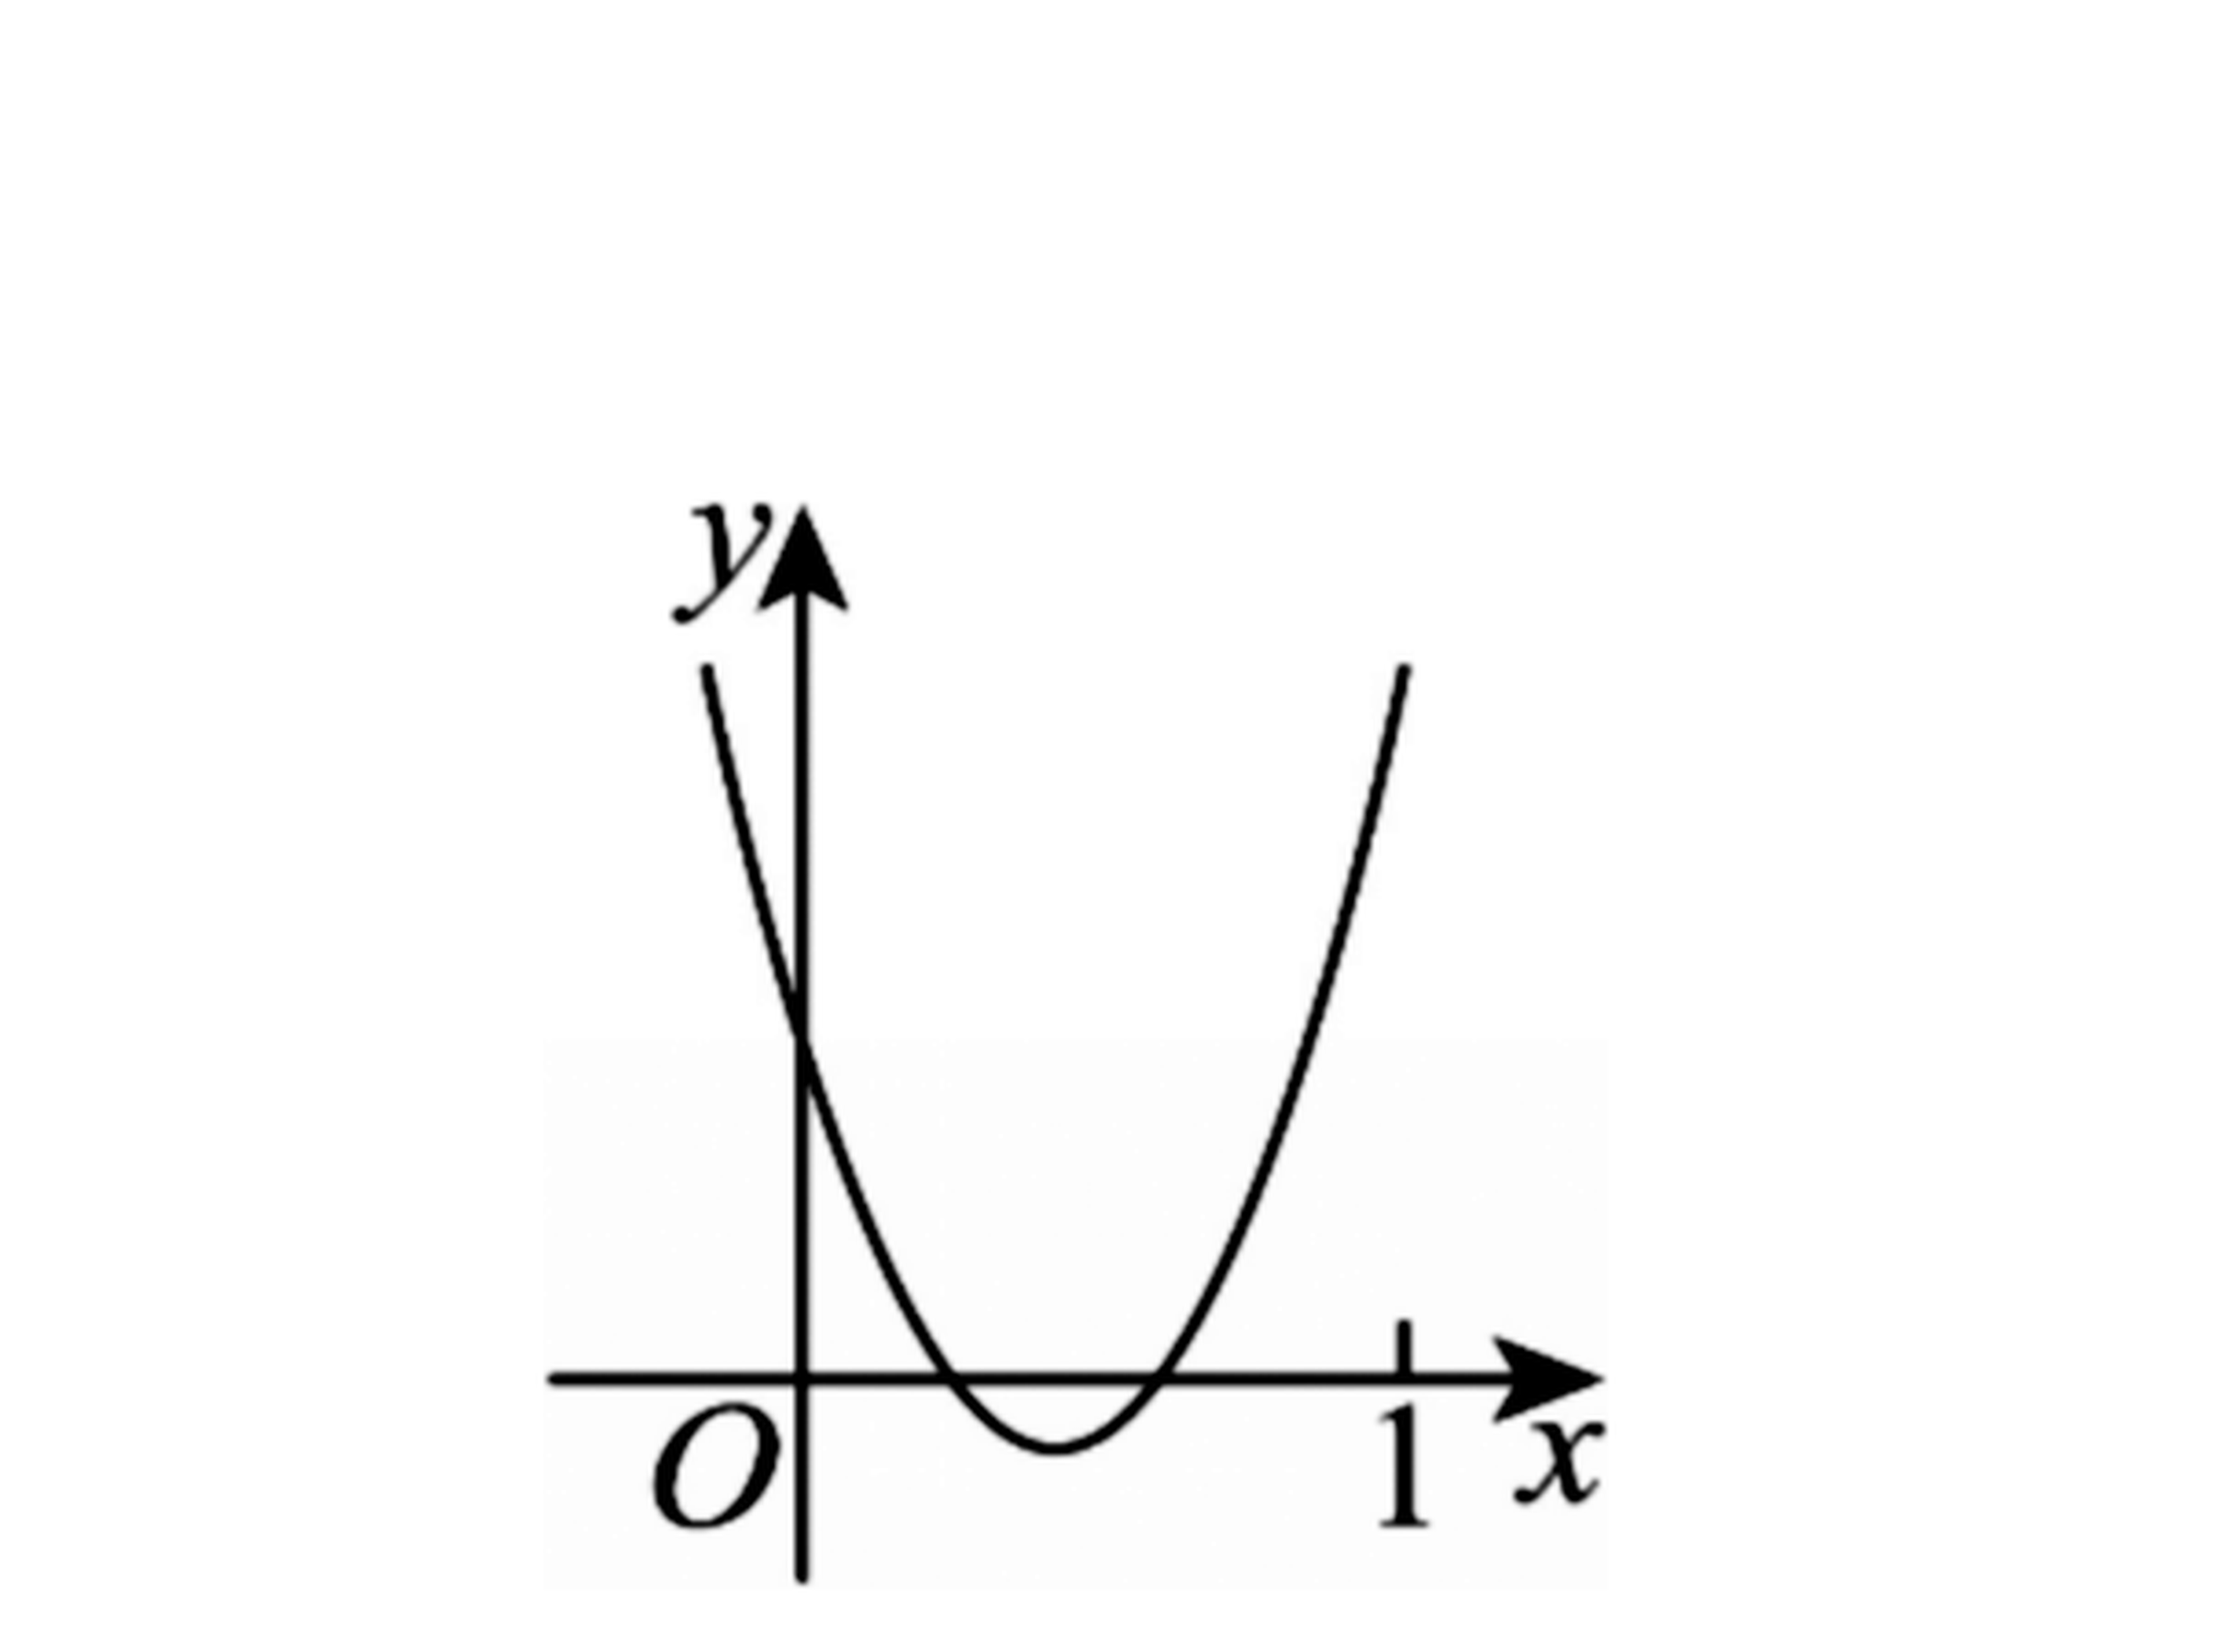
\includegraphics[width=0.32\textwidth]{figures/gao154_q15_stem.png}
\end{center}

\keepwithprev
\begin{center}
% 四幅指数函数图像选项取 05 页上半，按原卷 2×2 排布合并为一张，去粉色水印、去色、4× LANCZOS 放大；三版都出
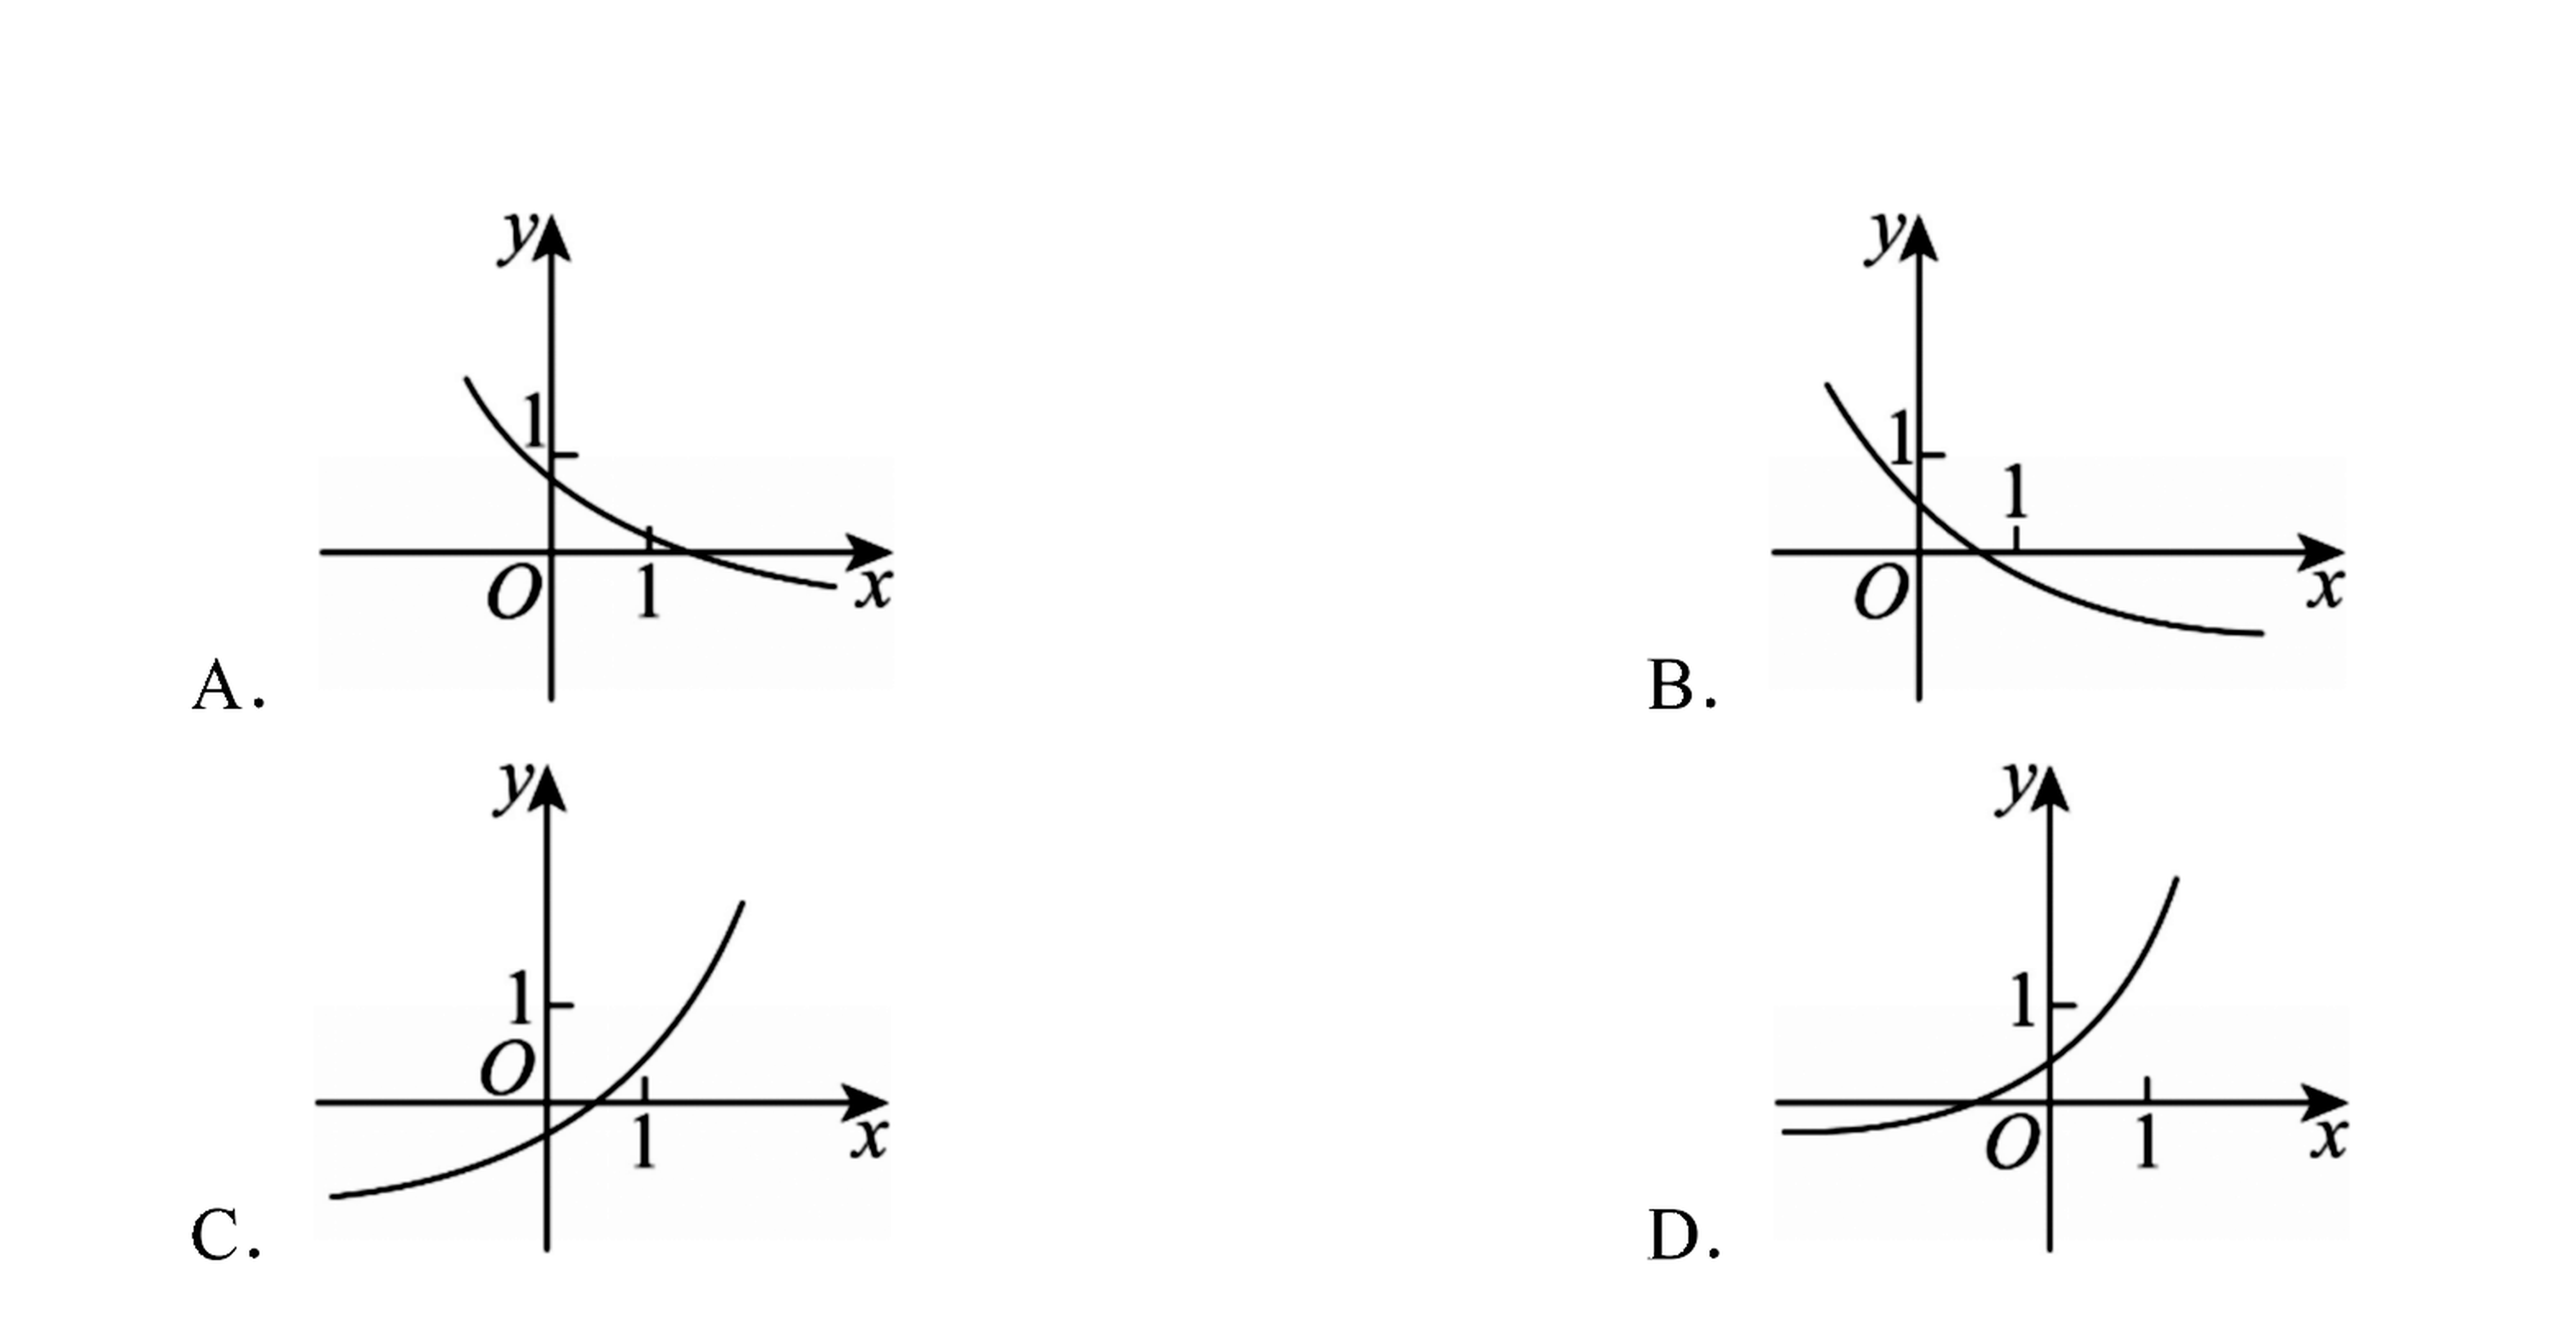
\includegraphics[width=0.80\textwidth]{figures/gao154_q15_opts.png}
\end{center}

\ifanswer
\solbegin
\step{由题意得 $0<a<b<1$，所以 $g(x)=a^x-b$ 在定义域 $\R$ 上严格减.}
\step{$g(0)=a^0-b=1-b>0$，$g(1)=a^1-b=a-b<0$，故 B 符合题意.}
\step{故选 $B$.}
\solend
\fi

% === Q16 === 高斯取整；解析 13 行，故选 C
\item 设 $[a]$ 表示不超过 $a$ 的最大整数，如 $[1.2]=1$，$[-3.2]=-4$，若 $x$、$y$、$z$ 为正实数，则 $\left[\dfrac{y+z}{x}\right]+\left[\dfrac{z+x}{y}\right]+\left[\dfrac{x+y}{z}\right]$ 的最小值为\mbox{（\quad）}

\keepwithprev
A. 2\qquad\qquad B. 3\qquad\qquad C. 4\qquad\qquad D. 6

\ifanswer
\solbegin
\step{若 $x$、$y$、$z$ 为正实数，}
\step{结合基本不等式得 $\dfrac{y+z}{x}+\dfrac{z+x}{y}+\dfrac{x+y}{z}=\dfrac yx+\dfrac xy+\dfrac zx+\dfrac xz+\dfrac zy+\dfrac yz$}
\step{$\geqslant2\sqrt{\dfrac yx\cdot\dfrac xy}+2\sqrt{\dfrac zx\cdot\dfrac xz}+2\sqrt{\dfrac zy\cdot\dfrac yz}=6$，当且仅当 $x=y=z$ 时取等号，}
\step{即 $\dfrac{y+z}{x}$，$\dfrac{z+x}{y}$，$\dfrac{x+y}{z}$ 中至少有一个不小于 2，不妨设 $\dfrac{y+z}{x}\geqslant\dfrac{z+x}{y}\geqslant\dfrac{x+y}{z}$，}
\step{$[a]$ 表示不超过 $a$ 的最大整数和 $\dfrac{y+z}{x}$，$\dfrac{z+x}{y}$，$\dfrac{x+y}{z}$ 中至少有一个不小于 2，}% 原卷此行把两句连写，照录未改（见 ⑤ 3）
\step{得 $\left[\dfrac{y+z}{x}\right]\geqslant2$，所以 $\left[\dfrac{y+z}{x}\right]+\left[\dfrac{z+x}{y}\right]+\left[\dfrac{x+y}{z}\right]\geqslant2$，}
\step{假设 $\left[\dfrac{y+z}{x}\right]+\left[\dfrac{z+x}{y}\right]+\left[\dfrac{x+y}{z}\right]$ 的最小值为 2，$\left[\dfrac{y+z}{x}\right]=2$，$\left[\dfrac{z+x}{y}\right]+\left[\dfrac{x+y}{z}\right]=0$，}
\step{所以 $2\leqslant\dfrac{y+z}{x}<3$，$0<\dfrac{z+x}{y}<1$，$0<\dfrac{x+y}{z}<1$，所以 $2<\dfrac{y+z}{x}+\dfrac{z+x}{y}+\dfrac{x+y}{z}<5$，}
\step{与 $\dfrac{y+z}{x}+\dfrac{z+x}{y}+\dfrac{x+y}{z}\geqslant6$ 矛盾，假设不成立，A 错误；}
\step{假设 $\left[\dfrac{y+z}{x}\right]+\left[\dfrac{z+x}{y}\right]+\left[\dfrac{x+y}{z}\right]$ 的最小值为 3，}
\step{则 $\left[\dfrac{y+z}{x}\right]=2$，$\left[\dfrac{z+x}{y}\right]=1$，$\left[\dfrac{x+y}{z}\right]=0$ 或 $\left[\dfrac{y+z}{x}\right]=3$，$\left[\dfrac{z+x}{y}\right]=\left[\dfrac{x+y}{z}\right]=0$，}
\step{同理可得 $3<\dfrac{y+z}{x}+\dfrac{z+x}{y}+\dfrac{x+y}{z}<6$，显然不成立，B 错误；}
\step{假设 $\left[\dfrac{y+z}{x}\right]+\left[\dfrac{z+x}{y}\right]+\left[\dfrac{x+y}{z}\right]$ 的最小值为 4，易得 $4<\dfrac{y+z}{x}+\dfrac{z+x}{y}+\dfrac{x+y}{z}<7$，}
\step{若取 $x=100$，$y=103$，$z=104$，则 $\left[\dfrac{y+z}{x}\right]=2$，$\left[\dfrac{z+x}{y}\right]=1$，$\left[\dfrac{x+y}{z}\right]=1$，}
\step{即 $\left[\dfrac{y+z}{x}\right]+\left[\dfrac{z+x}{y}\right]+\left[\dfrac{x+y}{z}\right]=4$，假设成立，C 正确，D 错误.}
\step{故选 $C$.}
\solend
\fi

\end{enumerate}

\bigsec{三、解答题}

\begin{enumerate}
\setcounter{enumi}{16}

% === Q17 === $B\subset A$ 单线照录；cases 块；解析 5 行
\item 设集合 $A=\{x\mid x^2+2x-3<0\}$，集合 $B=\{x\mid\lvert x+a\rvert<1\}$.

(1) 若 $a=3$，求 $A\cup B$；

(2) 设命题 $p:x\in A$，命题 $q:x\in B$，若 $p$ 是 $q$ 成立的必要不充分条件，求实数 $a$ 的取值范围.

\ifanswer
\solbegin
\step{(1) $A=(-3,1)$，}
\step{当 $a=3$ 时，$\lvert x+3\rvert<1$，解得 $-4<x<-2$，所以 $B=(-4,-2)$，}
\step{所以 $A\cup B=(-4,1)$.}
\step{(2) 因为 $p$ 是 $q$ 成立的必要不充分条件，所以 $B\subset A$.}
\step{因为 $A=(-3,1)$，$B=(-a-1,-a+1)$，所以 $\begin{cases}-a-1\geqslant-3\\-a+1<1\end{cases}$ 或 $\begin{cases}-a-1>-3\\-a+1\leqslant1\end{cases}$，解得 $0\leqslant a\leqslant2$.}
\solend
\fi

% === Q18 === 判别式 \Delta 两处照录；解析 9 行
\item 已知关于 $x$ 的一元二次方程 $x^2-mx+4m^2-3=0$ 的两个实根分别为 $x_1,x_2$.

(1) 若 $x_1,x_2$ 满足 $x_1+x_2=x_1x_2$，求实数 $m$ 的值；

(2) 求 $x_1^2+x_2^2$ 的最小值.

\ifanswer
\solbegin
\step{(1) 由韦达定理 $x_1+x_2=m$，$x_1x_2=4m^2-3$，}
\step{$\Delta=m^2-4(4m^2-3)=-15m^2+12\geqslant0$，即 $m^2\leqslant\dfrac45$.}
\step{由 $x_1+x_2=x_1x_2$ 得 $m=4m^2-3$，即 $4m^2-m-3=0$，}
\step{解得 $m=1$ 或 $m=-\dfrac34$.}
\step{$m=1$ 时 $m^2=1>\dfrac45$，$\Delta<0$，舍去；}
\step{$m=-\dfrac34$ 时 $m^2=\dfrac9{16}<\dfrac45$，符合，故 $m=-\dfrac34$.}
\step{(2) $x_1^2+x_2^2=(x_1+x_2)^2-2x_1x_2=m^2-2(4m^2-3)=-7m^2+6$，}
\step{函数 $y=-7m^2+6$ 开口向下，对称轴为 $m=0$，}% 原卷此处称求「最小值」，实为闭区间 $m^2\le\frac45$ 上的最小值，照录未改（见 ⑤ 4）
\step{故 $y_{\min}=-7\cdot\dfrac45+6=-\dfrac{28}{5}+\dfrac{30}{5}=\dfrac25$.}
\solend
\fi

% === Q19 === 全称命题；cases 块；解析 9 行
\item 设命题 $p$：对任意 $x\in\R$，不等式 $2mx^2+2mx+1>0$ 恒成立，$q:m\in\{m\mid\log_2(m-1)<1\}$.

(1) 若 $p$ 为真命题，求实数 $m$ 的取值范围；

(2) 若命题 $p$、$q$ 有且只有一个是真命题，求实数 $m$ 的取值范围.

\ifanswer
\solbegin
\step{(1) 由 $p$ 为真命题，得 $\forall x\in\R$，不等式 $2mx^2+2mx+1>0$ 恒成立，}
\step{当 $m=0$ 时，$1>0$ 恒成立；}
\step{当 $m\ne0$ 时，$\begin{cases}2m>0\\\Delta=4m^2-8m<0\end{cases}$，解得 $0<m<2$；}
\step{综上，$0\leqslant m<2$，即 $m$ 的取值范围是 $[0,2)$；}
\step{(2) 若 $q$ 为真，则有 $\log_2(m-1)<1$，得 $0<m-1<2$，解得 $1<m<3$，}
\step{因此命题 $q:m\in\{m\mid1<m<3\}$，由 (1) 得命题 $p:\{m\mid0\leqslant m<2\}$，}
\step{而命题 $p$、$q$ 有且只有一个是真命题，}
\step{当 $p$ 真 $q$ 假时，$\begin{cases}0\leqslant m<2\\m\leqslant1\text{ 或 }m\geqslant3\end{cases}$，解得 $0\leqslant m\leqslant1$，}
\step{当 $p$ 假 $q$ 真时，$\begin{cases}m<0\text{ 或 }m\geqslant2\\1<m<3\end{cases}$，解得 $2\leqslant m<3$，}
\step{故实数 $m$ 的取值范围是 $\{m\mid0\leqslant m\leqslant1\text{ 或 }2\leqslant m<3\}$.}
\solend
\fi

% === Q20 === Labubu 成本题；解析 10 行
\item Labubu 公司拟在 2027 年初推出智能机器人系列玩偶（单位：套）. 根据以往经验，其中一条生产线每月生产 $x$ 套玩具的成本 $P$ 由两部分费用（单位：元）构成：

(i) 固定成本（与生产玩具套数 $x$ 无关），总计 160000 元；

(ii) 每生产 $x$ 套需另投入的生产成本 $c(x)$ 元，其中 $c(x)=10x+\dfrac1{100}x^2$.

(1) 假设该生产线每月生产出的玩具能全部售出，问：该生产线每月生产玩具多少套时，可使得平均每套所需成本费用最少？此时每套玩具的成本费用是多少？

(2) 假设该生产线每月生产出的玩具能全部售出，但随着 $x$ 的增大，每月生产所需的直接总成本在急剧增加，因此售价也需随着 $x$ 的增大而适当增加. 设每套玩具的售价为 $q(x)$ 元，$q(x)=a+\dfrac xb$（$a,b\in\R$）. 若当月产量为 10000 套时利润最大，此时每套售价为 150 元，试求 $a,b$ 的值.（利润=销售收入$-$成本费用）

\ifanswer
\solbegin
\step{(1) 每月总成本 $P=160000+10x+\dfrac1{100}x^2$，}
\step{平均每套成本为 $\dfrac Px=\dfrac{160000}{x}+10+\dfrac x{100}\geqslant10+2\sqrt{\dfrac{160000}{x}\cdot\dfrac x{100}}=90$.}
\step{等号成立当且仅当 $\dfrac{160000}{x}=\dfrac x{100}$ 时，即 $x=4000$ 时取等号，}
\step{所以每月生产 4000 套时平均每套成本最少，此时每套成本为 90 元.}
\step{(2) 利润 $W(x)=x\cdot q(x)-P=\left(\dfrac1b-\dfrac1{100}\right)x^2+(a-10)x-160000$.}
\step{要在 $x=10000$ 处取得最大值，需 $\dfrac1b-\dfrac1{100}<0$，且对称轴为 $x=10000$，}
\step{故 $-\dfrac{a-10}{2\left(\frac1b-\frac1{100}\right)}=10000$，即 $a-10=-20000\left(\dfrac1b-\dfrac1{100}\right)$.}
\step{又 $q(10000)=a+\dfrac{10000}{b}=150$.}
\step{令 $t=\dfrac1b$，则 $a=150-10000t$，}
\step{代入上式 $140-10000t=-20000t+200$，解得 $t=\dfrac3{500}$，即 $b=\dfrac{500}{3}$；}
\step{再由 $a=150-10000\times\dfrac3{500}=150-60=90$，所以 $a=90$，$b=\dfrac{500}{3}$.}
\solend
\fi

% === Q21 === $A^+$／$A^-$ 新定义；$A\subseteq$ 带下划线照录、\varnothing；解析 16 行
\item 设集合 $A$ 为非空数集，定义 $A^+=\{x\mid x=a+b,a,b\in A\}$，$A^-=\{x\mid x=\lvert a-b\rvert,a,b\in A\}$.

(1) 若集合 $A=\{-1,1\}$，写出集合 $A^+$ 及 $A^-$；

(2) 若集合 $A=\{x_1,x_2,x_3,x_4\}$，$x_1<x_2<x_3<x_4$，且 $A^-=A$，求证：$x_1+x_4=x_2+x_3$；

(3) 若集合 $A\subseteq\{x\mid0\leqslant x\leqslant2020,x\in\N\}$，且 $A^+\cap A^-=\varnothing$，求集合 $A$ 元素的个数的最大值.

\ifanswer
\solbegin
\step{(1) 由 $A=\{-1,1\}$，得 $A^+=\{-2,0,2\}$，$A^-=\{0,2\}$；}
\step{(2) 由于集合 $A=\{x_1,x_2,x_3,x_4\}$，$x_1<x_2<x_3<x_4$，且 $A^-=A$，}
\step{所以 $A^-$ 中也只包含四个元素，即 $A^-=\{0,x_2-x_1,x_3-x_1,x_4-x_1\}$，}
\step{剩下的 $x_3-x_2=x_4-x_3=x_2-x_1$，所以 $x_1+x_4=x_2+x_3$；}
\step{(3) 设 $A=\{a_1,a_2,\cdots,a_k\}$ 满足题意，其中 $a_1<a_2<\cdots<a_k$，}
\step{则 $2a_1<a_1+a_2<a_1+a_3<\cdots<a_1+a_k<a_2+a_k<a_3+a_k<\cdots<a_{k-1}+a_k<2a_k$，所以 $\lvert A^+\rvert\geqslant2k-1$，}
\step{且 $a_1-a_1<a_2-a_1<a_3-a_1<\cdots<a_k-a_1$，所以 $\lvert A^-\rvert\geqslant k$，}
\step{因为 $A^+\cap A^-=\varnothing$，所以 $\lvert A^+\cup A^-\rvert=\lvert A^+\rvert+\lvert A^-\rvert\geqslant3k-1$，}
\step{$A^+\cup A^-$ 中最小的元素为 0，最大的元素为 $2a_k$，所以 $\lvert A^+\cup A^-\rvert\leqslant2a_k+1$，}
\step{所以 $3k-1\leqslant2a_k+1\leqslant4041$（$k\in\N^*$），所以 $k\leqslant1347$，}
\step{实际上当 $A=\{674,675,676,\cdots,2020\}$ 时满足题意，证明如下：}
\step{设 $A=\{m,m+1,m+2,\cdots,2020\}$，$m\in\N$，}
\step{则 $A^+=\{2m,2m+1,2m+2,\cdots,4040\}$，$A^-=\{0,1,2,\cdots,2020-m\}$，}
\step{由题意得 $2020-m<2m$，即 $m>673\dfrac13$，}
\step{故 $m$ 的最小值为 674，于是当 $m=674$ 时，$A$ 中元素最多，}
\step{即 $A=\{674,675,676,\cdots,2020\}$ 时满足题意，}
\step{综上所述，集合 $A$ 中元素的个数的最大值是 1347.}
\solend
\fi

\end{enumerate}

\bigsec{附加题}

\begin{enumerate}

% === 附加题 1 === 另起编号 1；「n 元集和集」弯引号；解析 6 行
\item 设集合 $A=\{a_1,a_2,a_3,a_4\}$，$C=\{2,3,4,6\}$，新定义：集合 $A$ 中所有含 $n$ 个元素的子集中 $n$ 个元素之和的不同值组成的集合为“$n$ 元集和集”. 若 $A$ 的“3 元集和集”为 $C$，则集合 $A=$\blankline[4.4em].

\ifanswer
\solbegin
\step{集合 $A$ 的 3 元子集共有 4 个：$\{a_1,a_2,a_3\}$，$\{a_1,a_2,a_4\}$，$\{a_1,a_3,a_4\}$，$\{a_2,a_3,a_4\}$，}
\step{集合 $C=\{a_1+a_2+a_3,a_1+a_2+a_4,a_1+a_3+a_4,a_2+a_3+a_4\}$，}
\step{不妨令 $a_1<a_2<a_3<a_4$，}
\step{则 $a_1+a_2+a_3<a_1+a_2+a_4<a_1+a_3+a_4<a_2+a_3+a_4$，}
\step{而 $C=\{2,3,4,6\}$，因此 $\begin{cases}a_1+a_2+a_3=2\\a_1+a_2+a_4=3\\a_1+a_3+a_4=4\\a_2+a_3+a_4=6\end{cases}$，相加化简得 $a_1+a_2+a_3+a_4=5$，}
\step{解得 $a_1=-1$，$a_2=1$，$a_3=2$，$a_4=3$，所以 $A=\{-1,1,2,3\}$.}
\solend
\fi

% === 附加题 2 === 解析配图（仅答案版出）；四选项；解析 15 行，故选 A
\item 已知函数 $f(x)=\log_p x+q$，其中 $p>0$ 且 $p\ne1$，曲线 $y=f(x)$ 经过 $P(1,2)$、$Q(2,3)$ 两点. 设 $g(x)=f(x)\cdot[f(x)-2]$，若 $\lvert g(a)\rvert=\lvert g(b)\rvert=\lvert g(c)\rvert=\lvert g(d)\rvert$，且 $a<b<c<d$，则 $ad(b+c)$ 的取值范围为\mbox{（\quad）}

\keepwithprev
A. $\left(\dfrac14,\dfrac5{16}\right)$\qquad B. $\left(\dfrac18,\dfrac5{16}\right)$\qquad C. $\left(\dfrac14,\dfrac25\right)$\qquad D. $\left(\dfrac18,\dfrac25\right)$

\ifanswer
\solbegin
\step{函数 $f(x)=\log_p x+q$，且曲线 $y=f(x)$ 经过点 $P(1,2)$ 和 $Q(2,3)$，}
\step{所以 $\begin{cases}f(1)=q=2\\f(2)=\log_p2+q=3\end{cases}$，解得 $p=2$，$q=2$，$f(x)=\log_2 x+2$.}
\step{不妨设 $\lvert g(x)\rvert=k$，令 $\log_2 x=m$，则 $f(x)\cdot[f(x)-2]=m(m+2)=m^2+2m$，}
\step{画出函数 $y=\lvert m^2+2m\rvert$ 的图象，如图所示，}
\begin{center}
% $y=|m(m+2)|$ 图像取 11 页右上，去粉色水印、去色、4× LANCZOS 放大；仅答案版出
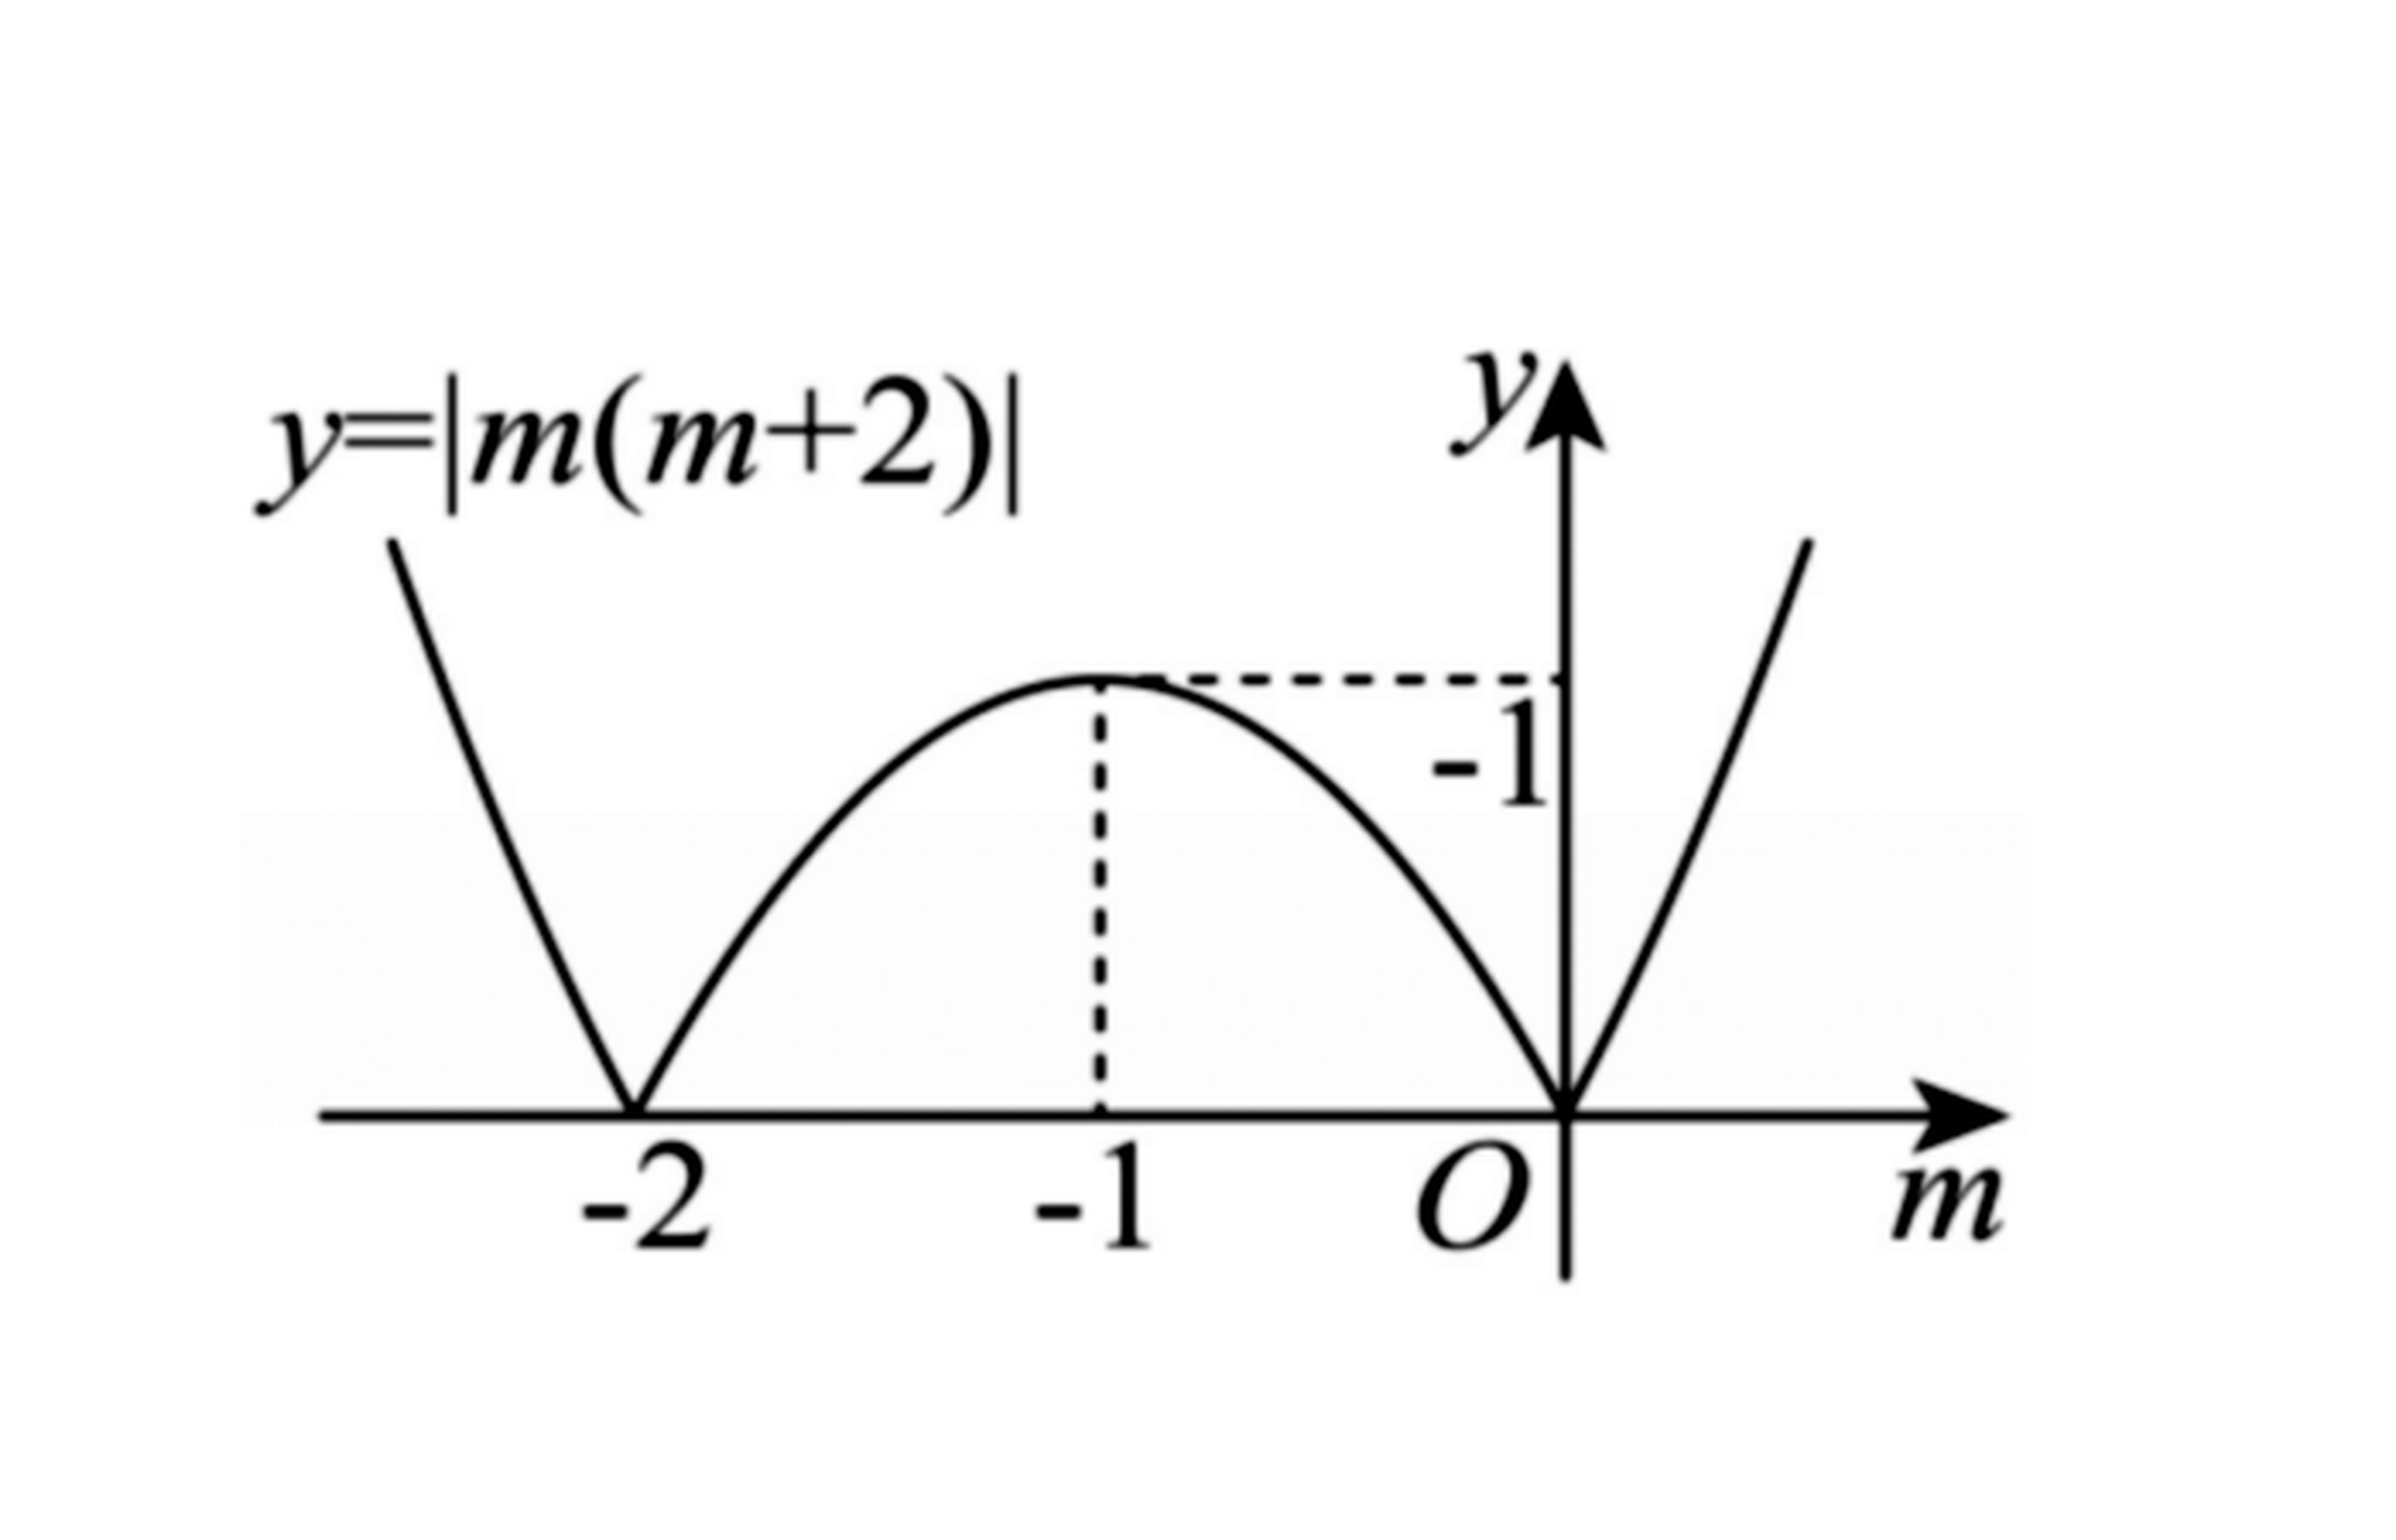
\includegraphics[width=0.46\textwidth]{figures/gao154_fujia2.png}
\end{center}
\step{由图像得 $k\in(0,1)$，}
\step{所以方程 $m^2+2m=k$ 和 $m^2+2m=-k$ 各有两个不同的根，}
\step{其中方程 $m^2+2m-k=0$ 的两根为 $m=-1\pm\sqrt{1+k}$，}
\step{方程 $m^2+2m+k=0$ 的两根为 $m=-1\pm\sqrt{1-k}$，}
\step{所以 $m_1=-1-\sqrt{1+k}$，$m_2=-1-\sqrt{1-k}$，$m_3=-1+\sqrt{1-k}$，$m_4=-1+\sqrt{1+k}$，且 $m_1<m_2<m_3<m_4$，}
\step{由 $m=\log_2 x$，则 $x=2^m$，}
\step{所以 $a=2^{-1-\sqrt{1+k}}$，$b=2^{-1-\sqrt{1-k}}$，$c=2^{-1+\sqrt{1-k}}$，$d=2^{-1+\sqrt{1+k}}$，}
\step{所以 $ad=2^{-1-\sqrt{1+k}}\times2^{-1+\sqrt{1+k}}=2^{(-1-\sqrt{1+k})+(-1+\sqrt{1+k})}=2^{-2}=\dfrac14$，}
\step{$b+c=2^{-1-\sqrt{1-k}}+2^{-1+\sqrt{1-k}}=\dfrac{2^{-\sqrt{1-k}}+2^{\sqrt{1-k}}}{2}$，}
\step{令 $s=\sqrt{1-k}$，其中 $s\in(0,1)$，则 $b+c=\dfrac12\left(2^{-s}+2^s\right)$，}
\step{设函数 $y=2^s+\dfrac1{2^s}$，令 $r=2^s\in(1,2)$，所以 $y=r+\dfrac1r$ 在 $(1,2)$ 上严格增，}
\step{所以函数 $y=2^s+\dfrac1{2^s}$ 在 $(0,1)$ 上严格增，所以 $y=2^s+\dfrac1{2^s}\in\left(2,\dfrac52\right)$，}
\step{所以 $b+c=\dfrac{2^{-s}+2^s}{2}\in\left(1,\dfrac54\right)$，$ad(b+c)=\dfrac{b+c}{4}\in\left(\dfrac14,\dfrac5{16}\right)$，}
\step{所以 $ad(b+c)$ 的取值范围是 $\left(\dfrac14,\dfrac5{16}\right)$，故选 $A$.}
\solend
\fi

\end{enumerate}

\end{document}
"
%
% ① 原始材料：微信公众号"魔都数学加油站"文章，连载"27学年高一154"，原文标题
% "27学年高一154——2026-2027年上海市徐汇中学高一上期中"；
% 原文链接：https://mp.weixin.qq.com/s/Qs2T7Zwsug-KKFE2wefDUg 。
% 正文为 12 张 PNG 页（01/03/04/05/07/11/12 为 2560×3620，
% 02/06/08/09/10 为 4762×6735，同一篇各页分辨率混排，逐页按各自分辨率裁图核对）。
% 体例：讲评版——一、填空题 3—12（10 题）、二、选择题 13—16（4 题）、
% 三、解答题 17—21（5 题）、附加题 1—2（2 题，原卷**另起编号**"1." "2."，
% 不与正题连号，同 高一a 成例），共 21 题；全卷每题均印【解析】
% （逐题核实，见 ② ②）。题目、答案、解析均据原图转录；卷面粉红色水印
% "魔都数学加油站"及公众号页脚未录入。
% 全卷插图清单（逐页通读 12 页确认）：3 组——
%   · Q15 题干配图（$f(x)=(x-a)(x-b)$ 抛物线，04 页右下：x/y 轴、O、1、
%     开口向上两零点均在 (0,1) 内），三版都出，裁 figures/gao154_q15_stem.png；
%   · Q15 四幅图像选项（05 页上半 2×2 排布，A/B/C/D 四幅指数函数图像，
%     合并成一张，照 高一136 Q13/Q22 成例），三版都出，
%     裁 figures/gao154_q15_opts.png；
%   · 附加题第 2 题解析配图（$y=\lvert m(m+2)\rvert$ 图像，11 页右上：
%     W 形折线、$-2$、$-1$、O、虚线 $y=1$ 与 $m=-1$），仅答案版出，
%     裁 figures/gao154_fujia2.png；
%   3 图均取自原卷截图，去粉色水印、去色、4× LANCZOS 放大；Q15 题干图
%   左侧题干残字"的图"已裁白。其余各页逐页确认无其它题目配图、无表格；
%   12 页下半仅水印、无正文。
%
% 卷首标题：原卷印作"2026-2027 年徐汇中学高一上期中"，年份区间按全稿惯例排 en dash；
% 原卷卷面未印副标题，本稿按同期中卷知识模块口径补出"集合与常用逻辑用语、不等式、函数"。
%
% ② 与原卷的排版差异：
%   ① 原文从第 3 题起，本稿保留原题号；共 21 题四节，正题到 21，附加题另起编号
%      1—2（\bigsec{附加题} 后 \begin{enumerate} 不 \setcounter，同 高一a 成例）；
%   ② 全 21 题均印【解析】、用 \solbegin…\solend，无只印【答案】或答案印括号内的题；
%      四道正题选择题答案在解析末句"故选 C／A／B／C"（Q13—Q16）、附加题第 2 题
%      答案在解析末句"故选 A"，括号 \mbox{（\quad）} 留空、不另提 \ans{}；
%      答案版【答案】/【解析】标记数 = 21 = 全卷题数；
%   ③ 原卷卷面未印副标题，本稿按知识模块口径补出；
%   ④ 原卷填空横线按全稿惯例排 \blankline[4.4em]；选择题括号排 \mbox{（\quad）}、
%      四道正题选择题与附加题第 2 题的选项段前按惯例各加 \keepwithprev
%      （Q15 与附加题 2 的选项段是整块图，\keepwithprev 后接 \begin{center}）；
%      解答题不留作答区、不加 \anspace（原卷为讲评版）；
%   ⑤ 数集黑板粗体：Q4"$x,y\in R$"、Q9"$x\in\R$"、Q13 无、
%      Q15"定义域 $\R$"、Q19"$\forall x\in\R$"、Q21"$x\in\N$"与"$k\in\N^*$"、
%      Q20"$a,b\in\R$"、附加题 2 无——原卷印斜体或正体粗体 R/N/N*，
%      按全稿惯例归一 \R／\N／\N^*；绝对值排 \lvert…\rvert
%      （Q5、Q9、Q12、Q13、Q16、Q21、附加题 2），集合描述竖线排 \mid
%      （Q5、Q17、Q19、Q21），不等号按全稿惯例排 \leqslant／\geqslant；
%      空集 \varnothing（Q21 题干 (3)）；
%   ⑥ 子集符号逐处照录、不得统一：Q6 题干印"$\{1,2\}\subset M\subseteq\{1,2,3,4,5\}$"
%      （前单线 ⊂、后带下划线 ⊆，同句两形并用），解析亦两形并用；
%      Q17 解析 (2)"$B\subset A$"印单线 ⊂；Q21 题干 (3)"$A\subseteq\{x\mid\cdots\}$"
%      印带下划线 ⊆——逐处放大核，分别 \subset／\subseteq，照录未统一（见 ④）；
%   ⑦ 判别式 Δ/△：Q18 解析 (1)"$\Delta=m^2-4(4m^2-3)$"与 Q19 解析 (1)
%      "$\Delta=4m^2-8m<0$"两处均印等腰偏高粗三角、照录 \Delta；本卷无扁等边
%      细线 \triangle 用例（见 ④）；
%   ⑧ 中文弯引号照录：Q4"设 $x$、$y\in\R$. 若 $x+y>2$，则 $x>1$ 或 $y>1$"、
%      附加题 1"$n$ 元集和集"与"3 元集和集"；注释里一律 ASCII 引号；
%      数学式内 CJK 用 \text{}（Q5 解集描述"或"、Q19 集合描述的"或"）；
%   ⑨ "图像／图象"逐处放大核：Q15 题干与解析印"图象"（象，无亻）、
%      Q16 无、附加题 2 解析印"图象"与"图像"（"画出函数…的图象"、
%      "由图像得"——两形并用，逐处照录未统一）；Q13/Q14 无数集图像字样；
%      半角逗号在数学组之间是全稿惯例、非笔误，逐处照录（Q3、Q10、Q16、
%      Q18、Q20、Q21 的 $x_1,x_2$ 之类）；行末西文句点 ASCII `.`；
%      行中全角逗号／顿号照录（Q6"3，4，5"、Q20"（单位：元）"、
%      附加题 1"$a_1,a_2,a_3,a_4$"）；
%   ⑩ 复杂式照录别简化：Q3 $a^{\frac{12}{7}}\cdot\left(\frac17\right)^{\frac17}
%      \cdot\sqrt[7]{a^4}$ 与 $7^{-\frac17}a^{\frac{16}{7}}$、Q7 $x^{-m}$、
%      Q8 $\frac{b-2a+2}{2a}$、Q11 $\frac{9+4\sqrt2}{6}$、Q12 $506\frac29$ 与
%      $506\frac49$、Q16 高斯取整 $[a]$、Q20 $c(x)=10x+\frac1{100}x^2$ 与
%      $q(x)=a+\frac xb$、Q21 $A^+$／$A^-$ 与 $|A^+|\geqslant2k-1$、
%      附加题 2 $m=-1\pm\sqrt{1+k}$ 与 $ad(b+c)$；
%      \left…\right 不得拆到不同 $…$ 组（Q5 $\left\{x\mid\cdots\right\}$、
%      Q20 $\left(\frac1b-\frac1{100}\right)$、附加题 2 $\left(\frac14,\frac5{16}\right)$）；
%      cases 块一律 \begin{cases}…\end{cases}；
%   ⑪ 一条 \step = 原卷解析的一个印刷行，cases 块整体算一个印刷行；别并折行、
%      别拆行。Q11 九行、Q12 六行、Q16 十六行、Q20 十一行、Q21 十七行、
%      附加题 2 十八行均按印刷行逐条断，不丢行；
%   ⑫ 配图：Q15 题干小图（三版都出）放 \item 内题干之后 \begin{center}，
%      Q15 四幅选项图（三版都出）放 \keepwithprev 之后的 \begin{center}，
%      Q15 用 \needvspace 守卫把"题干＋两图"整块推走（守卫放 \item 之前，
%      见 高一145 Q14/Q20 与 高一136 Q13 成例）；附加题 2 解析配图（仅答案版出）
%      放 \ifanswer 内 \solbegin…\solend 的 \step 之间（高一73 第 16 题成例）；
%   ⑬ 原卷解析内无红色"法一／法二"之类小标题，故本卷无 \stepm；红色水印
%      "魔都数学加油站"不录入；
%   ⑭ 跨页续印按题合并：见 ⑥；
%
% ③ 行数复核：一条 \step = 原卷解析的一个印刷行，cases 块作一个印刷行计。
%   逐题数（主会话逐页核对定稿）：Q3：1；Q4：1；Q5：3；Q6：4；Q7：3；
%   Q8：1；Q9：5；Q10：4；Q11：9；Q12：6；Q13：5；Q14：4；Q15：3；
%   Q16：16；Q17：5；Q18：9；Q19：10；Q20：11；Q21：17；
%   附加题 1：6；附加题 2：18。
%   合计 141 条 \step（本卷无 \stepm），与原卷逐题印刷行相等。全卷 21 题
%   均设 \solbegin…\solend，答案版【答案】/【解析】标记数 = 21 = 全卷题数。
%
% ④ 判别式／子集符号结论（逐处放大原图照录、不得统一，主会话像素级复核）：
%   判别式：Q18 解析 (1)"$\Delta=m^2-4(4m^2-3)=-15m^2+12\geqslant0$"、
%      Q19 解析 (1)"$\Delta=4m^2-8m<0$"共 2 处，逐处放大确认印等腰偏高
%      粗三角（高>宽、右斜边粗），照录 \Delta；本卷无扁等边细线 \triangle
%      用例，无几何三角形符号。
%   子集：Q6 题干"$\{1,2\}\subset M\subseteq\{1,2,3,4,5\}$"前 ⊂ 单线、
%      后 ⊆ 带下划线（/tmp/gao154/z/zoom/q6_subset.png），解析两处同样两形
%      并用，分别照录 \subset／\subseteq；Q17 解析 (2)"$B\subset A$"单线
%      照录 \subset；Q21 题干 (3)"$A\subseteq\{x\mid\cdots\}$"带下划线
%      照录 \subseteq。本卷 ⊂ 与 ⊆ 混用逐处照录、不得统一。
%      空集 \varnothing（Q21 题干 (3)）、数集 \R／\N／\N^* 归一见 ② ⑤。
%
% ⑤ 存疑照录（放大原图确认，照录未改、正文对应处另有 % 注）：
%   1. Q7 题干印 $f(x)=(3m-1)x^{-m}$，解析首句却写"幂函数 $f(x)=x^\alpha$
%      的系数必须为 1"（用 $\alpha$ 作指数记号），随后 $f(2)=2^\alpha=8$
%      得 $\alpha=3$、$f(x)=x^3$——题干指数 $-m$ 与解析 $\alpha$ 记法不同，
%      系原卷记号前后不一，逐处照录未统一（放大 01/02 页确认）。
%   2. Q11 解析"因为 $u>0,v>0$，由基本不等式得 $\frac{4v}{u}+\frac{2u}{v}
%      \geqslant2\sqrt{\frac{4v}{u}\cdot\frac{2u}{v}}=4\sqrt2$"与
%      "所以 $\frac4u+\frac1v=\frac16\left(\frac4u+\frac1v\right)(2u+v)$"
%      照录，未把 $u,v$ 化简回 $x,y$。
%   3. Q16 解析把"$[a]$ 表示不超过 $a$ 的最大整数"与"和至少有一个不小于 2"
%      连写在同一行（原卷如此），照录未改；末行"假设成立，C 正确，D 错误"照录。
%   4. Q18 解析 (2)"函数 $y=-7m^2+6$ 开口向下，对称轴为 $m=0$"却称求
%      "$y_{\min}$"（实为在 $m^2\leqslant\frac45$ 闭区间上的最小值），
%      照录未改。
%   5. Q20 题干"$q(x)=a+\frac xb$（$a,b\in\R$）"与解析
%      "$W(x)=\left(\frac1b-\frac1{100}\right)x^2+(a-10)x-160000$"照录；
%      末行解得 $a=90,b=\frac{500}{3}$ 照录未化简。
%   6. Q21 题干 (3)"$A\subseteq\{x\mid0\leqslant x\leqslant2020,x\in\N\}$"
%      与解析"$3k-1\leqslant2a_k+1\leqslant4041$（$k\in\N^*$）"照录；
%      末行"集合 $A$ 中元素的个数的最大值是 1347"照录。
%   7. 附加题 1 解析"相加化简得 $a_1+a_2+a_3+a_4=5$"照录；
%      附加题 2 解析"由图像得 $k\in(0,1)$"与"由图像得"／"的图象"两形
%      并用逐处照录（见 ② ⑨）；末行"$ad(b+c)$ 的取值范围是
%      $\left(\frac14,\frac5{16}\right)$，故选 A"照录。
%   全卷除此 7 类外未发现其它笔误／自相矛盾处；21 题均印【解析】、
%   无只印【答案】或答案印括号内的题（见 ② ②）。
%
% ⑥ 跨页续印按题合并说明（逐页核实定稿）：Q3—Q5 题干＋解析在 01 页
%   （Q5 解析末 2 行续 01 页下半）；Q6、Q7 题干＋解析在 01 页下半
%   （Q7 解析余 2 行续 02 页顶）；Q8、Q9 题干＋解析在 02 页上半
%   （Q9 解析余 3 行续 02 页下半）；Q10 题干＋解析在 02 页下半；
%   Q11 题干＋解析前 6 行在 03 页上半、余 3 行续 03 页下半；
%   Q12 题干＋解析前 5 行在 03 页下半、末行续 04 页顶；"二、选择题"
%   标题与 Q13 题干＋选项＋解析在 04 页上半；Q14 题干＋选项＋解析、
%   Q15 题干＋题干配图在 04 页下半；Q15 四幅选项图＋解析、
%   Q16 题干＋选项＋解析首行在 05 页上半，Q16 解析余 12 行在
%   05 页下半—06 页上半；"三、解答题"标题与 Q17 题干＋两问＋解析
%   在 06 页下半；Q18 题干＋两问＋解析在 07 页上半—下半；
%   Q19 题干＋两问＋解析首行在 07 页下半，解析余 8 行在 08 页上半；
%   Q20 题干在 08 页下半，解析 (1) 4 行＋(2) 首 4 行在 08 页下半—09 页上半，
%   (2) 余 2 行在 09 页下半；Q21 题干＋三问＋解析 (1)(2) 4 行在
%   09 页下半—10 页上半，解析 (3) 余 12 行在 10 页上半—下半；
%   "附加题"标题与附加题 1 题干＋解析首 3 行在 10 页下半，
%   余 3 行续 11 页上半；附加题 2 题干＋选项＋解析前 3 行在 11 页上半，
%   解析配图＋余 12 行在 11 页下半—12 页上半，末行
%   "所以 $ad(b+c)$ 的取值范围是 $\left(\frac14,\frac5{16}\right)$，故选 A"
%   为全卷收尾（12 页下半仅水印、无正文）。
%   本稿按题连排，不丢行、不并折行；全卷末题为附加题第 2 题。
%
\documentclass[a4paper,11pt]{article}
\usepackage{common}

\begin{document}

\examtitlest[3]{2026--2027 年徐汇中学高一上期中}{集合与常用逻辑用语、不等式、函数}

\bigsec{一、填空题}

\begin{enumerate}
\setcounter{enumi}{2}

% === Q3 === 分数指数幂照录；解析 1 行
\item 已知 $a>0$，化简 $a^{\frac{12}{7}}\cdot\left(\dfrac17\right)^{\frac17}\cdot\sqrt[7]{a^4}=$\blankline[4.4em].

\ifanswer
\solbegin
\step{$a^{\frac{12}{7}}\cdot\left(\dfrac17\right)^{\frac17}\cdot\sqrt[7]{a^4}=a^{\frac{12}{7}}\cdot(7^{-1})^{\frac17}\cdot a^{\frac47}=7^{-\frac17}a^{\frac{16}{7}}$.}
\solend
\fi

% === Q4 === 反证法；中文弯引号照录；解析 1 行
\item 用反证法证明命题：“设 $x$、$y\in\R$. 若 $x+y>2$，则 $x>1$ 或 $y>1$”时，假设的内容应该是\blankline[4.4em].

\ifanswer
\solbegin
\step{由反证法得，假设的内容应该是 $x\leqslant1$ 且 $y\leqslant1$.}
\solend
\fi

% === Q5 === 分式不等式；cases 块；解析 3 行
\item 不等式 $\dfrac{2x+3}{x-1}\geqslant1$ 的解集为\blankline[4.4em].

\ifanswer
\solbegin
\step{$\dfrac{2x+3}{x-1}\geqslant1$，即 $\dfrac{2x+3}{x-1}-1\geqslant0$，$\dfrac{x+4}{x-1}\geqslant0$，}
\step{等价于 $\begin{cases}(x+4)(x-1)\geqslant0\\x-1\ne0\end{cases}$，解得 $x>1$ 或 $x\leqslant-4$，}
\step{故解集为 $\{x\mid x>1\text{ 或 }x\leqslant-4\}$.}
\solend
\fi

% === Q6 === ⊂ 与 ⊆ 并用照录；解析 4 行
\item 满足条件 $\{1,2\}\subset M\subseteq\{1,2,3,4,5\}$ 的集合 $M$ 的个数为\blankline[4.4em].

\ifanswer
\solbegin
\step{因为 $\{1,2\}\subset M\subseteq\{1,2,3,4,5\}$，所以集合 $M$ 必含有元素 1，2，}
\step{且至少含有元素 3，4，5 中的一个，}
\step{则集合 $M$ 的个数与集合 $\{3,4,5\}$ 的非空子集的个数一样，}
\step{所以集合 $M$ 的个数为 $2^3-1=7$.}
\solend
\fi

% === Q7 === 题干 $x^{-m}$、解析用 $x^\alpha$ 记法，原卷记号差异照录（见 ⑤ 1）；解析 3 行
\item 已知幂函数 $f(x)=(3m-1)x^{-m}$，且 $f(2)=8$，则 $f(m)=$\blankline[4.4em].

\ifanswer
\solbegin
\step{幂函数 $f(x)=x^\alpha$ 的系数必须为 1，所以 $3m-1=1$，得 $m=\dfrac23$.}
\step{又 $f(2)=2^\alpha=8=2^3$，故 $\alpha=3$，即 $f(x)=x^3$，}
\step{所以 $f(m)=f\left(\dfrac23\right)=\left(\dfrac23\right)^3=\dfrac8{27}$.}
\solend
\fi

% === Q8 === 换底公式；解析 1 行
\item 已知 $a=\lg2$，$b=\lg3$，用含 $a,b$ 的代数式表示 $\log_4 75=$\blankline[4.4em].

\ifanswer
\solbegin
\step{$\log_4 75=\dfrac{\lg\left(3\times\frac{10^2}{2^2}\right)}{\lg2^2}=\dfrac{\lg3+2-2\lg2}{2\lg2}=\dfrac{b-2a+2}{2a}$.}
\solend
\fi

% === Q9 === 三角不等式取等；解析 5 行
\item 设 $x\in\R$，则方程 $\lvert x-2\rvert+\lvert3x+1\rvert=\lvert2x+3\rvert$ 的解集是\blankline[4.4em].

\ifanswer
\solbegin
\step{由 $\lvert x-2\rvert=\lvert2-x\rvert$，故原方程可化为 $\lvert2-x\rvert+\lvert3x+1\rvert=\lvert2x+3\rvert$，}
\step{又 $(2-x)+(3x+1)=2x+3$，}
\step{由三角不等式 $\lvert2-x\rvert+\lvert3x+1\rvert\geqslant\lvert(2-x)+(3x+1)\rvert=\lvert2x+3\rvert$，}
\step{当且仅当 $(2-x)(3x+1)\geqslant0$ 等号成立，}
\step{解 $(2-x)(3x+1)\geqslant0$ 得 $-\dfrac13\leqslant x\leqslant2$，故原方程的解集为 $\left[-\dfrac13,2\right]$.}
\solend
\fi

% === Q10 === 韦达定理；cases 块；解析 4 行
\item 已知一元二次不等式 $x^2+bx+c>0$ 的解集为 $(-\infty,-1)\cup(2,+\infty)$，则一元二次不等式 $bx^2+cx-1<0$ 的解集是\blankline[4.4em].

\ifanswer
\solbegin
\step{因为 $x^2+bx+c>0$ 的解集为 $(-\infty,-1)\cup(2,+\infty)$，}
\step{所以方程 $x^2+bx+c=0$ 的两根为 $-1$ 和 2，则有 $\begin{cases}-b=-1+2\\c=-1\times2\end{cases}$，即 $\begin{cases}b=-1\\c=-2\end{cases}$，}
\step{则 $bx^2+cx-1<0$ 等价于 $-x^2-2x-1<0$，得 $x^2+2x+1>0$，得 $(x+1)^2>0$，}
\step{解得 $x\ne-1$，故不等式 $bx^2+cx-1<0$ 的解集为 $(-\infty,-1)\cup(-1,+\infty)$.}
\solend
\fi

% === Q11 === 换元 $u,v$；解析 9 行
\item 已知正数 $x,y$ 满足 $2x+y=1$，则 $\dfrac4{x+2}+\dfrac1{y+1}$ 的最小值为\blankline[4.4em].

\ifanswer
\solbegin
\step{令 $u=x+2$，$v=y+1$，则 $u>2$，$v>1$，}
\step{且 $2u+v=2(x+2)+(y+1)=2x+y+5=6$.}
\step{因为 $u>0$，$v>0$，由基本不等式得 $\dfrac{4v}{u}+\dfrac{2u}{v}\geqslant2\sqrt{\dfrac{4v}{u}\cdot\dfrac{2u}{v}}=4\sqrt2$，}
\step{所以 $\dfrac4u+\dfrac1v=\dfrac16\left(\dfrac4u+\dfrac1v\right)(2u+v)=\dfrac16\left(9+\dfrac{4v}{u}+\dfrac{2u}{v}\right)\geqslant\dfrac{9+4\sqrt2}{6}$，}
\step{当且仅当 $\dfrac{4v}{u}=\dfrac{2u}{v}$，即 $u=\sqrt2v$ 时等号成立，}
\step{与 $2u+v=6$ 联立得 $u=\dfrac{6\sqrt2}{2\sqrt2+1}$，$v=\dfrac6{2\sqrt2+1}$，}
\step{此时 $x=u-2=\dfrac{2\sqrt2-2}{2\sqrt2+1}>0$，$y=v-1=\dfrac{5-2\sqrt2}{2\sqrt2+1}>0$，且 $2x+y=1$，}
\step{满足题设，所以下界可以取得，}
\step{因此 $\dfrac4{x+2}+\dfrac1{y+1}$ 的最小值为 $\dfrac{9+4\sqrt2}{6}$.}
\solend
\fi

% === Q12 === 2025 个整数解；解析 6 行
\item 若关于 $x$ 的不等式 $\lvert x-2k\rvert+\lvert x-3k\rvert<4k$ 共有 2025 个整数解，则实数 $k$ 的取值范围为\blankline[4.4em].

\ifanswer
\solbegin
\step{显然 $k>0$，由 $\lvert x-2k\rvert+\lvert x-3k\rvert<4k$，得 $\dfrac12k<x<\dfrac92k$，}
\step{因为该不等式共有 2025 个整数解，所以 $2024<\dfrac{9k}{2}-\dfrac k2\leqslant2026$，}
\step{解得 $506<k\leqslant506.5$，}
\step{由 $\dfrac k2\in(253,253.25]$，得这 2025 个整数解只能为 254、255、256、$\cdots$、2278，}
\step{所以 $2278<\dfrac{9k}{2}\leqslant2279$，解得 $506\dfrac29<k\leqslant506\dfrac49$，结合 $506<k\leqslant506.5$，}
\step{得 $k$ 的取值范围是 $\left(506\dfrac29,506\dfrac49\right]$.}
\solend
\fi

\end{enumerate}

\bigsec{二、选择题}

\begin{enumerate}
\setcounter{enumi}{12}

% === Q13 === 四选项一行；解析 5 行，故选 C
\item 若 $a<b<0$，则下列不等式中不成立的是\mbox{（\quad）}

\keepwithprev
A. $a-b>a$\qquad B. $\dfrac1a>\dfrac1b$\qquad C. $a^3>b^3$\qquad D. $\lvert a\rvert>\lvert b\rvert$

\ifanswer
\solbegin
\step{A 选项，因为 $b<0$，所以 $-b>0$，不等式两边同加上 $a$ 得 $a-b>a$，故 A 正确；}
\step{B 选项，因为 $a<b<0$，所以 $ab>0$，不等式两边同除以 $ab$，则 $\dfrac1b<\dfrac1a<0$，故 B 正确；}
\step{C 选项，不妨设 $a=-2$，$b=-1$，则 $a^3=-8$，$b^3=-1$，故 $a^3<b^3$，故 C 错误；}
\step{D 选项，因为 $a<b<0$，所以 $-a>-b$，即 $\lvert a\rvert>\lvert b\rvert$，故 D 正确.}
\step{故选 $C$.}
\solend
\fi

% === Q14 === 选项两行两列；解析 4 行，故选 A
\item 设命题 $p:x^2-5x+4\ne0$，命题 $q:x\ne1$，则 $p$ 是 $q$ 的\mbox{（\quad）}条件

\keepwithprev
A. 充分不必要\qquad\qquad B. 必要不充分

C. 充要\qquad\qquad D. 既不充分也不必要

\ifanswer
\solbegin
\step{$p:x^2-5x+4\ne0\Leftrightarrow(x-1)(x-4)\ne0\Leftrightarrow x\ne1$ 且 $x\ne4$；$q:x\ne1$.}
\step{充分性：当 $x\ne1$ 且 $x\ne4$ 时，$x\ne1$，所以 $p\Rightarrow q$；}
\step{必要性：当 $x\ne1$ 时，若 $x=4$，此时 $p$ 不成立，即 $q\nRightarrow p$；}
\step{所以 $p$ 是 $q$ 的充分不必要条件，故选 $A$.}
\solend
\fi

% === Q15 === 题干配图（三版都出）+ 四幅图像选项（2×2 合并，三版都出）；守卫放 \item 之前；解析 3 行，故选 B
\needvspace{9cm}
\item 已知函数 $f(x)=(x-a)(x-b)$（$a<b$）的图象如图所示，则函数 $g(x)=a^x-b$ 的图象可能是\mbox{（\quad）}

\begin{center}
% 抛物线题干配图取 04 页右下，去粉色水印、去色、4× LANCZOS 放大；三版都出
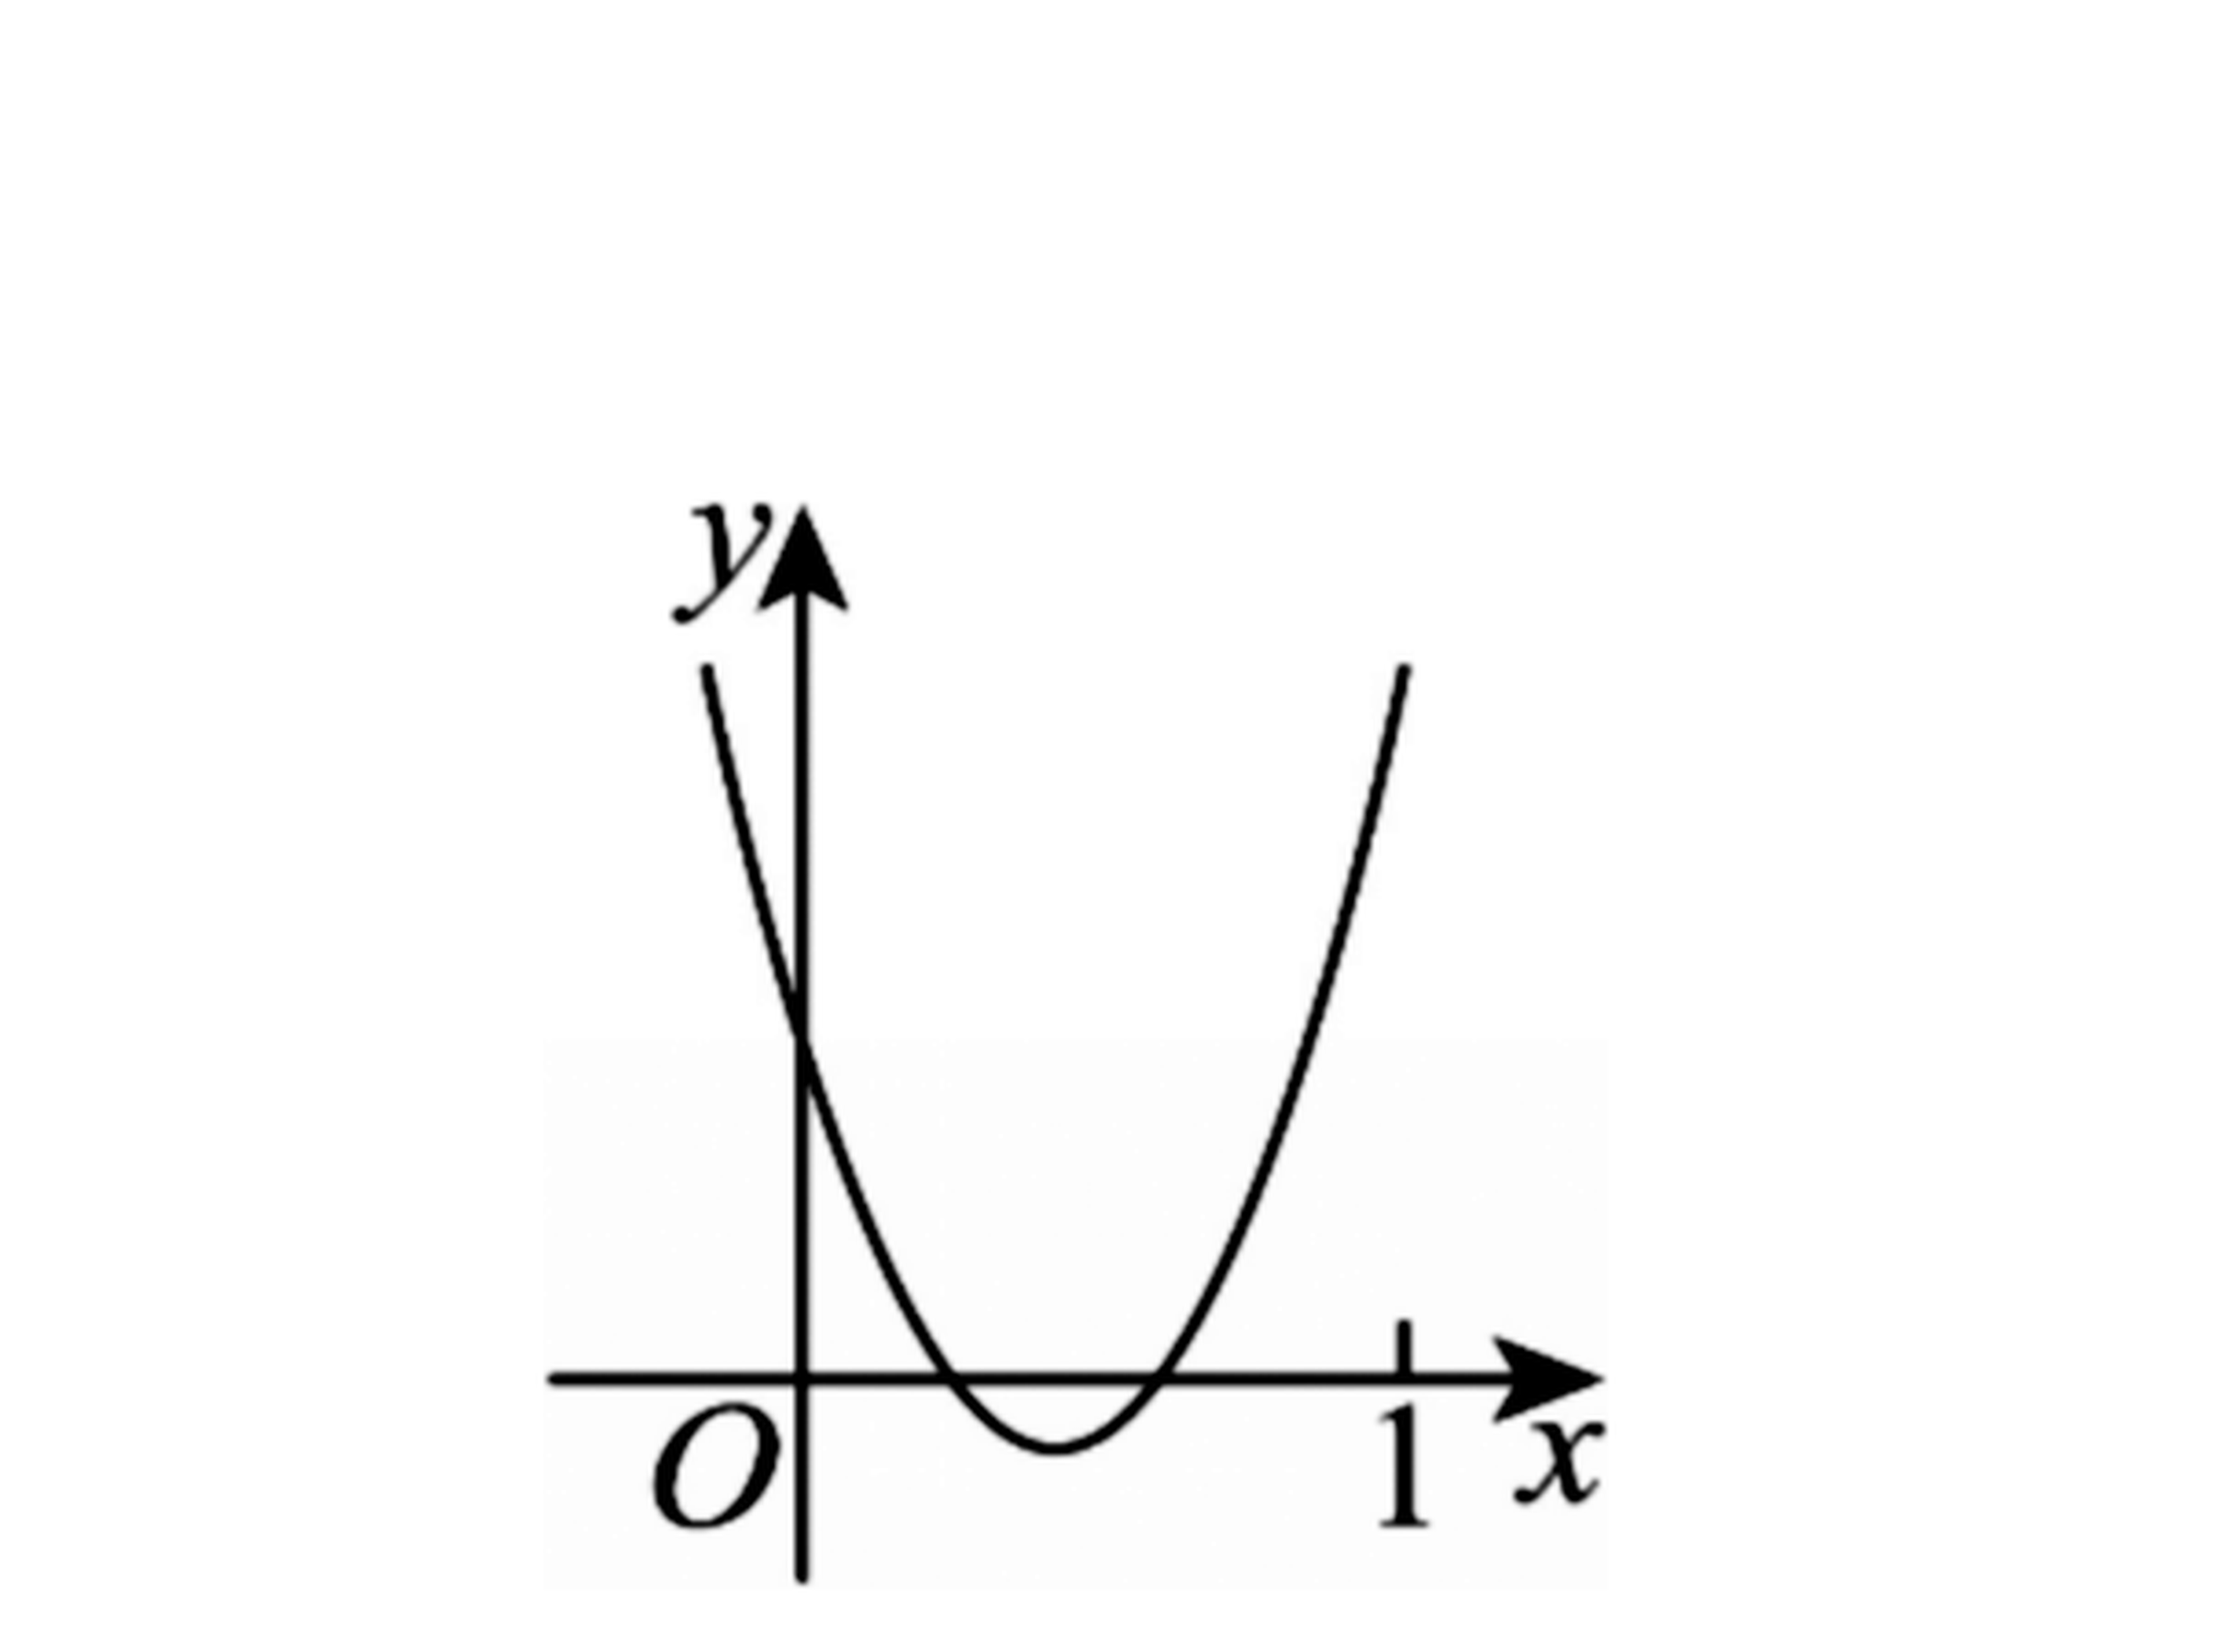
\includegraphics[width=0.32\textwidth]{figures/gao154_q15_stem.png}
\end{center}

\keepwithprev
\begin{center}
% 四幅指数函数图像选项取 05 页上半，按原卷 2×2 排布合并为一张，去粉色水印、去色、4× LANCZOS 放大；三版都出
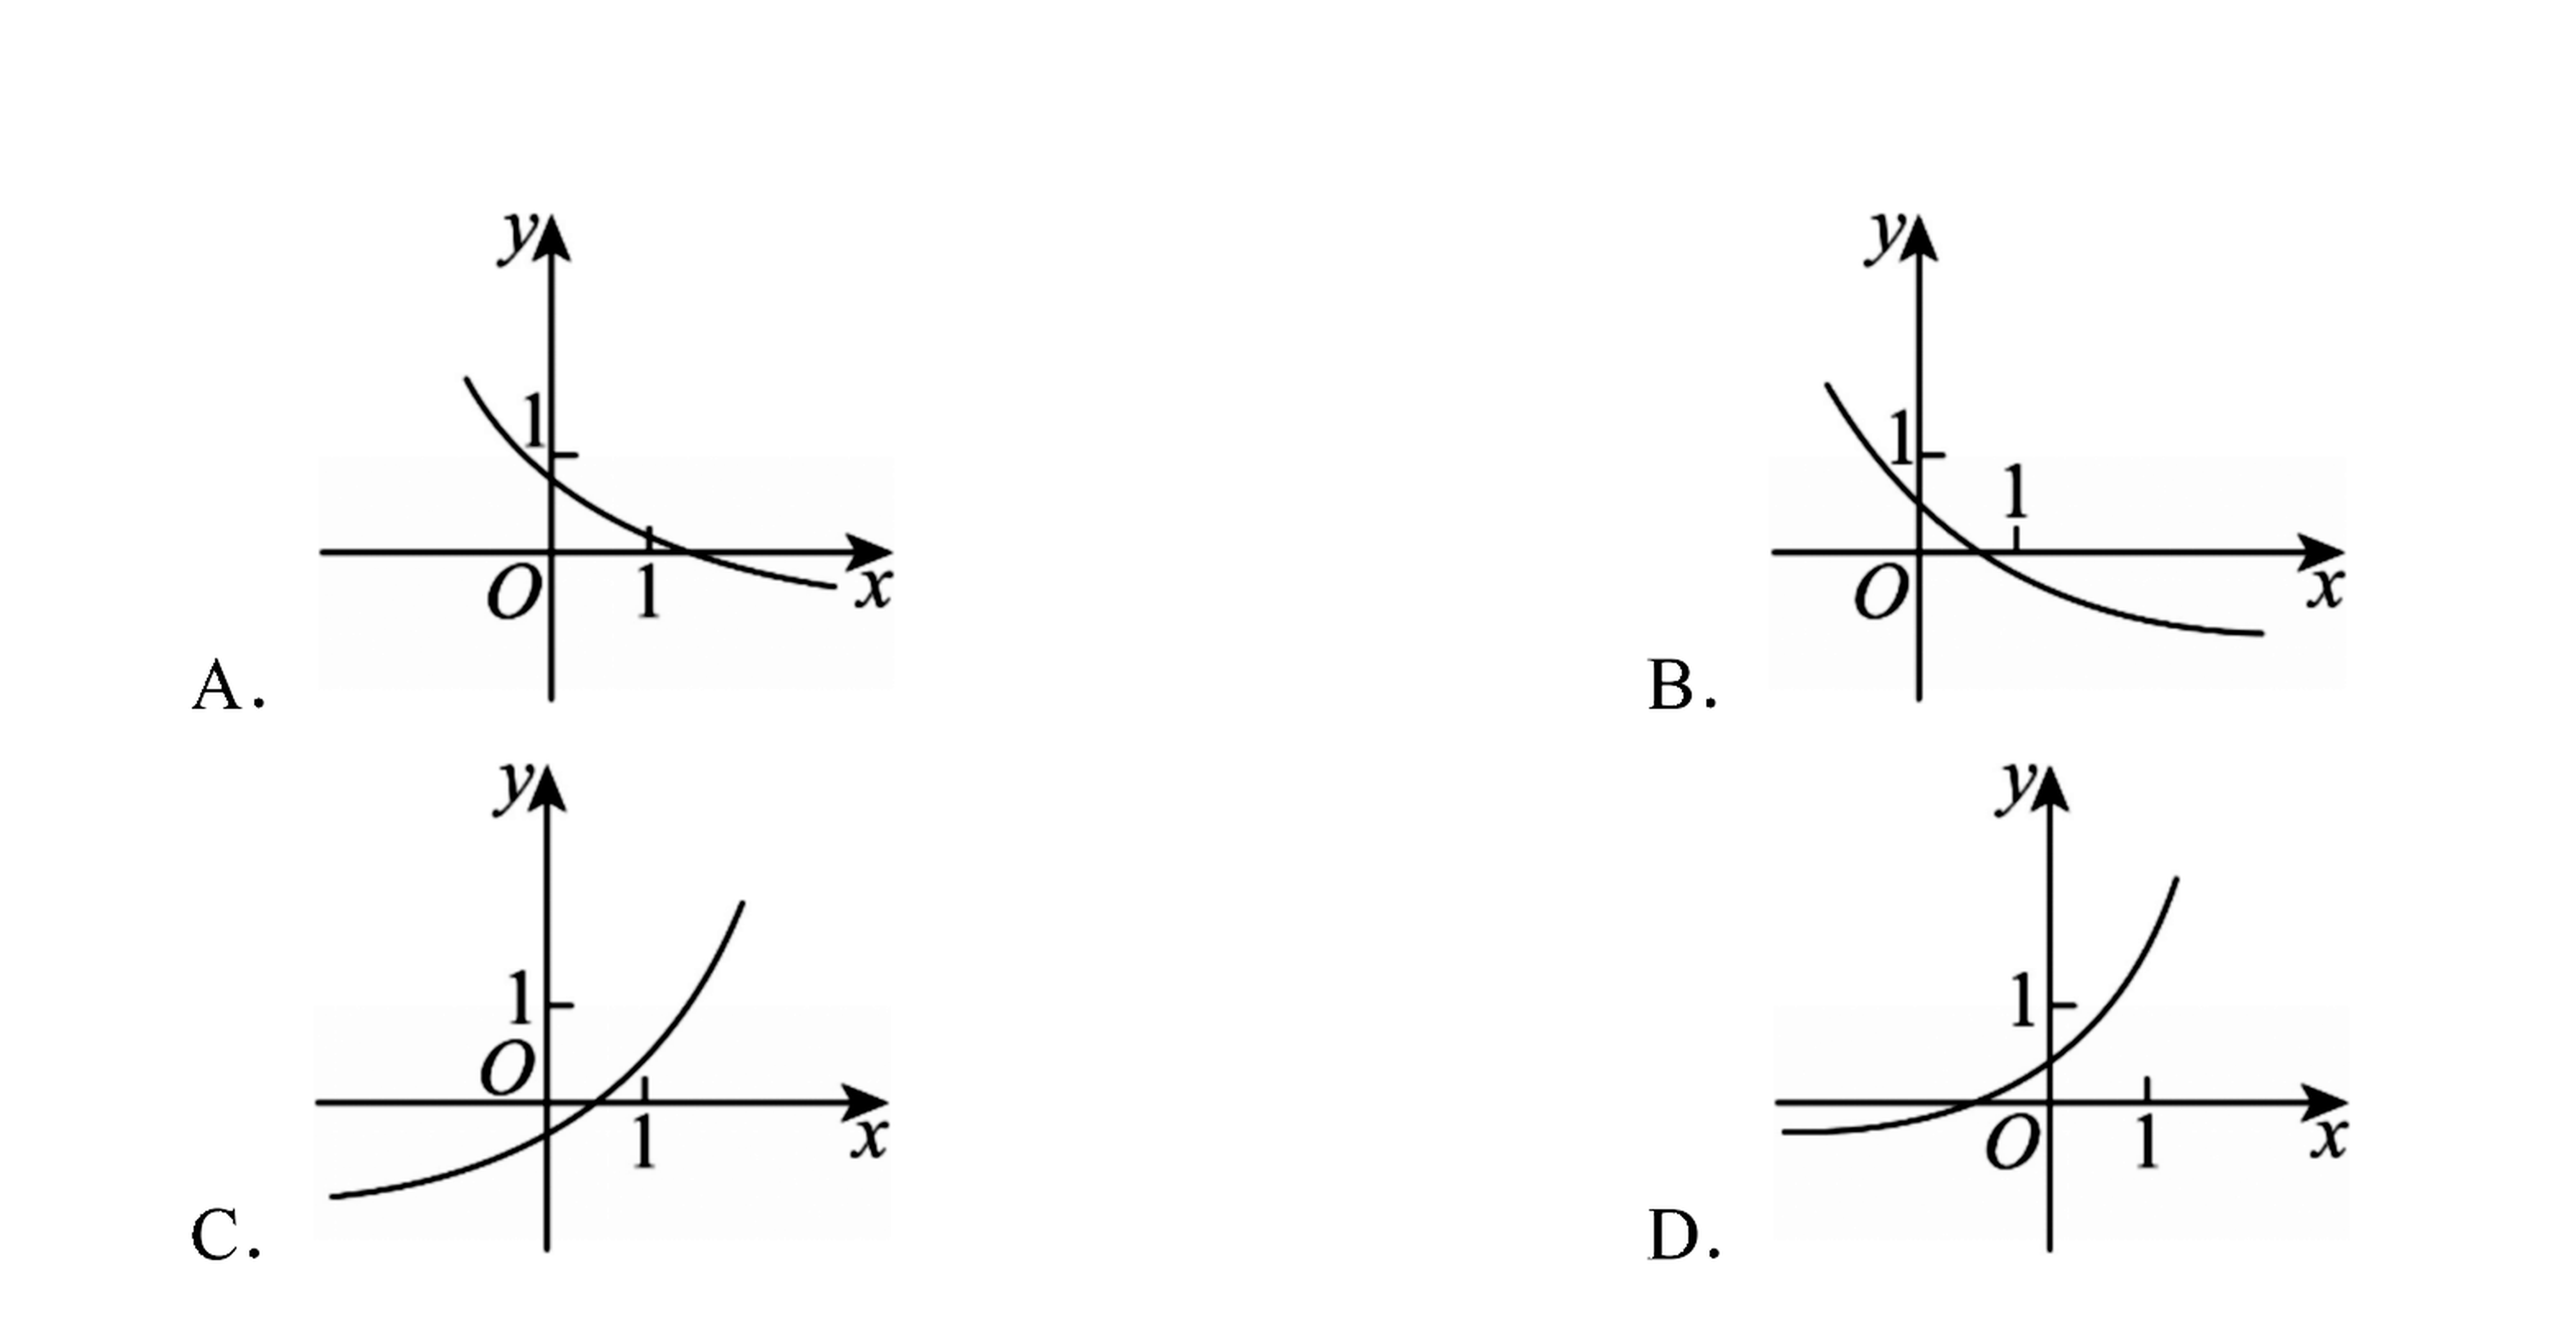
\includegraphics[width=0.80\textwidth]{figures/gao154_q15_opts.png}
\end{center}

\ifanswer
\solbegin
\step{由题意得 $0<a<b<1$，所以 $g(x)=a^x-b$ 在定义域 $\R$ 上严格减.}
\step{$g(0)=a^0-b=1-b>0$，$g(1)=a^1-b=a-b<0$，故 B 符合题意.}
\step{故选 $B$.}
\solend
\fi

% === Q16 === 高斯取整；解析 13 行，故选 C
\item 设 $[a]$ 表示不超过 $a$ 的最大整数，如 $[1.2]=1$，$[-3.2]=-4$，若 $x$、$y$、$z$ 为正实数，则 $\left[\dfrac{y+z}{x}\right]+\left[\dfrac{z+x}{y}\right]+\left[\dfrac{x+y}{z}\right]$ 的最小值为\mbox{（\quad）}

\keepwithprev
A. 2\qquad\qquad B. 3\qquad\qquad C. 4\qquad\qquad D. 6

\ifanswer
\solbegin
\step{若 $x$、$y$、$z$ 为正实数，}
\step{结合基本不等式得 $\dfrac{y+z}{x}+\dfrac{z+x}{y}+\dfrac{x+y}{z}=\dfrac yx+\dfrac xy+\dfrac zx+\dfrac xz+\dfrac zy+\dfrac yz$}
\step{$\geqslant2\sqrt{\dfrac yx\cdot\dfrac xy}+2\sqrt{\dfrac zx\cdot\dfrac xz}+2\sqrt{\dfrac zy\cdot\dfrac yz}=6$，当且仅当 $x=y=z$ 时取等号，}
\step{即 $\dfrac{y+z}{x}$，$\dfrac{z+x}{y}$，$\dfrac{x+y}{z}$ 中至少有一个不小于 2，不妨设 $\dfrac{y+z}{x}\geqslant\dfrac{z+x}{y}\geqslant\dfrac{x+y}{z}$，}
\step{$[a]$ 表示不超过 $a$ 的最大整数和 $\dfrac{y+z}{x}$，$\dfrac{z+x}{y}$，$\dfrac{x+y}{z}$ 中至少有一个不小于 2，}% 原卷此行把两句连写，照录未改（见 ⑤ 3）
\step{得 $\left[\dfrac{y+z}{x}\right]\geqslant2$，所以 $\left[\dfrac{y+z}{x}\right]+\left[\dfrac{z+x}{y}\right]+\left[\dfrac{x+y}{z}\right]\geqslant2$，}
\step{假设 $\left[\dfrac{y+z}{x}\right]+\left[\dfrac{z+x}{y}\right]+\left[\dfrac{x+y}{z}\right]$ 的最小值为 2，$\left[\dfrac{y+z}{x}\right]=2$，$\left[\dfrac{z+x}{y}\right]+\left[\dfrac{x+y}{z}\right]=0$，}
\step{所以 $2\leqslant\dfrac{y+z}{x}<3$，$0<\dfrac{z+x}{y}<1$，$0<\dfrac{x+y}{z}<1$，所以 $2<\dfrac{y+z}{x}+\dfrac{z+x}{y}+\dfrac{x+y}{z}<5$，}
\step{与 $\dfrac{y+z}{x}+\dfrac{z+x}{y}+\dfrac{x+y}{z}\geqslant6$ 矛盾，假设不成立，A 错误；}
\step{假设 $\left[\dfrac{y+z}{x}\right]+\left[\dfrac{z+x}{y}\right]+\left[\dfrac{x+y}{z}\right]$ 的最小值为 3，}
\step{则 $\left[\dfrac{y+z}{x}\right]=2$，$\left[\dfrac{z+x}{y}\right]=1$，$\left[\dfrac{x+y}{z}\right]=0$ 或 $\left[\dfrac{y+z}{x}\right]=3$，$\left[\dfrac{z+x}{y}\right]=\left[\dfrac{x+y}{z}\right]=0$，}
\step{同理可得 $3<\dfrac{y+z}{x}+\dfrac{z+x}{y}+\dfrac{x+y}{z}<6$，显然不成立，B 错误；}
\step{假设 $\left[\dfrac{y+z}{x}\right]+\left[\dfrac{z+x}{y}\right]+\left[\dfrac{x+y}{z}\right]$ 的最小值为 4，易得 $4<\dfrac{y+z}{x}+\dfrac{z+x}{y}+\dfrac{x+y}{z}<7$，}
\step{若取 $x=100$，$y=103$，$z=104$，则 $\left[\dfrac{y+z}{x}\right]=2$，$\left[\dfrac{z+x}{y}\right]=1$，$\left[\dfrac{x+y}{z}\right]=1$，}
\step{即 $\left[\dfrac{y+z}{x}\right]+\left[\dfrac{z+x}{y}\right]+\left[\dfrac{x+y}{z}\right]=4$，假设成立，C 正确，D 错误.}
\step{故选 $C$.}
\solend
\fi

\end{enumerate}

\bigsec{三、解答题}

\begin{enumerate}
\setcounter{enumi}{16}

% === Q17 === $B\subset A$ 单线照录；cases 块；解析 5 行
\item 设集合 $A=\{x\mid x^2+2x-3<0\}$，集合 $B=\{x\mid\lvert x+a\rvert<1\}$.

(1) 若 $a=3$，求 $A\cup B$；

(2) 设命题 $p:x\in A$，命题 $q:x\in B$，若 $p$ 是 $q$ 成立的必要不充分条件，求实数 $a$ 的取值范围.

\ifanswer
\solbegin
\step{(1) $A=(-3,1)$，}
\step{当 $a=3$ 时，$\lvert x+3\rvert<1$，解得 $-4<x<-2$，所以 $B=(-4,-2)$，}
\step{所以 $A\cup B=(-4,1)$.}
\step{(2) 因为 $p$ 是 $q$ 成立的必要不充分条件，所以 $B\subset A$.}
\step{因为 $A=(-3,1)$，$B=(-a-1,-a+1)$，所以 $\begin{cases}-a-1\geqslant-3\\-a+1<1\end{cases}$ 或 $\begin{cases}-a-1>-3\\-a+1\leqslant1\end{cases}$，解得 $0\leqslant a\leqslant2$.}
\solend
\fi

% === Q18 === 判别式 \Delta 两处照录；解析 9 行
\item 已知关于 $x$ 的一元二次方程 $x^2-mx+4m^2-3=0$ 的两个实根分别为 $x_1,x_2$.

(1) 若 $x_1,x_2$ 满足 $x_1+x_2=x_1x_2$，求实数 $m$ 的值；

(2) 求 $x_1^2+x_2^2$ 的最小值.

\ifanswer
\solbegin
\step{(1) 由韦达定理 $x_1+x_2=m$，$x_1x_2=4m^2-3$，}
\step{$\Delta=m^2-4(4m^2-3)=-15m^2+12\geqslant0$，即 $m^2\leqslant\dfrac45$.}
\step{由 $x_1+x_2=x_1x_2$ 得 $m=4m^2-3$，即 $4m^2-m-3=0$，}
\step{解得 $m=1$ 或 $m=-\dfrac34$.}
\step{$m=1$ 时 $m^2=1>\dfrac45$，$\Delta<0$，舍去；}
\step{$m=-\dfrac34$ 时 $m^2=\dfrac9{16}<\dfrac45$，符合，故 $m=-\dfrac34$.}
\step{(2) $x_1^2+x_2^2=(x_1+x_2)^2-2x_1x_2=m^2-2(4m^2-3)=-7m^2+6$，}
\step{函数 $y=-7m^2+6$ 开口向下，对称轴为 $m=0$，}% 原卷此处称求「最小值」，实为闭区间 $m^2\le\frac45$ 上的最小值，照录未改（见 ⑤ 4）
\step{故 $y_{\min}=-7\cdot\dfrac45+6=-\dfrac{28}{5}+\dfrac{30}{5}=\dfrac25$.}
\solend
\fi

% === Q19 === 全称命题；cases 块；解析 9 行
\item 设命题 $p$：对任意 $x\in\R$，不等式 $2mx^2+2mx+1>0$ 恒成立，$q:m\in\{m\mid\log_2(m-1)<1\}$.

(1) 若 $p$ 为真命题，求实数 $m$ 的取值范围；

(2) 若命题 $p$、$q$ 有且只有一个是真命题，求实数 $m$ 的取值范围.

\ifanswer
\solbegin
\step{(1) 由 $p$ 为真命题，得 $\forall x\in\R$，不等式 $2mx^2+2mx+1>0$ 恒成立，}
\step{当 $m=0$ 时，$1>0$ 恒成立；}
\step{当 $m\ne0$ 时，$\begin{cases}2m>0\\\Delta=4m^2-8m<0\end{cases}$，解得 $0<m<2$；}
\step{综上，$0\leqslant m<2$，即 $m$ 的取值范围是 $[0,2)$；}
\step{(2) 若 $q$ 为真，则有 $\log_2(m-1)<1$，得 $0<m-1<2$，解得 $1<m<3$，}
\step{因此命题 $q:m\in\{m\mid1<m<3\}$，由 (1) 得命题 $p:\{m\mid0\leqslant m<2\}$，}
\step{而命题 $p$、$q$ 有且只有一个是真命题，}
\step{当 $p$ 真 $q$ 假时，$\begin{cases}0\leqslant m<2\\m\leqslant1\text{ 或 }m\geqslant3\end{cases}$，解得 $0\leqslant m\leqslant1$，}
\step{当 $p$ 假 $q$ 真时，$\begin{cases}m<0\text{ 或 }m\geqslant2\\1<m<3\end{cases}$，解得 $2\leqslant m<3$，}
\step{故实数 $m$ 的取值范围是 $\{m\mid0\leqslant m\leqslant1\text{ 或 }2\leqslant m<3\}$.}
\solend
\fi

% === Q20 === Labubu 成本题；解析 10 行
\item Labubu 公司拟在 2027 年初推出智能机器人系列玩偶（单位：套）. 根据以往经验，其中一条生产线每月生产 $x$ 套玩具的成本 $P$ 由两部分费用（单位：元）构成：

(i) 固定成本（与生产玩具套数 $x$ 无关），总计 160000 元；

(ii) 每生产 $x$ 套需另投入的生产成本 $c(x)$ 元，其中 $c(x)=10x+\dfrac1{100}x^2$.

(1) 假设该生产线每月生产出的玩具能全部售出，问：该生产线每月生产玩具多少套时，可使得平均每套所需成本费用最少？此时每套玩具的成本费用是多少？

(2) 假设该生产线每月生产出的玩具能全部售出，但随着 $x$ 的增大，每月生产所需的直接总成本在急剧增加，因此售价也需随着 $x$ 的增大而适当增加. 设每套玩具的售价为 $q(x)$ 元，$q(x)=a+\dfrac xb$（$a,b\in\R$）. 若当月产量为 10000 套时利润最大，此时每套售价为 150 元，试求 $a,b$ 的值.（利润=销售收入$-$成本费用）

\ifanswer
\solbegin
\step{(1) 每月总成本 $P=160000+10x+\dfrac1{100}x^2$，}
\step{平均每套成本为 $\dfrac Px=\dfrac{160000}{x}+10+\dfrac x{100}\geqslant10+2\sqrt{\dfrac{160000}{x}\cdot\dfrac x{100}}=90$.}
\step{等号成立当且仅当 $\dfrac{160000}{x}=\dfrac x{100}$ 时，即 $x=4000$ 时取等号，}
\step{所以每月生产 4000 套时平均每套成本最少，此时每套成本为 90 元.}
\step{(2) 利润 $W(x)=x\cdot q(x)-P=\left(\dfrac1b-\dfrac1{100}\right)x^2+(a-10)x-160000$.}
\step{要在 $x=10000$ 处取得最大值，需 $\dfrac1b-\dfrac1{100}<0$，且对称轴为 $x=10000$，}
\step{故 $-\dfrac{a-10}{2\left(\frac1b-\frac1{100}\right)}=10000$，即 $a-10=-20000\left(\dfrac1b-\dfrac1{100}\right)$.}
\step{又 $q(10000)=a+\dfrac{10000}{b}=150$.}
\step{令 $t=\dfrac1b$，则 $a=150-10000t$，}
\step{代入上式 $140-10000t=-20000t+200$，解得 $t=\dfrac3{500}$，即 $b=\dfrac{500}{3}$；}
\step{再由 $a=150-10000\times\dfrac3{500}=150-60=90$，所以 $a=90$，$b=\dfrac{500}{3}$.}
\solend
\fi

% === Q21 === $A^+$／$A^-$ 新定义；$A\subseteq$ 带下划线照录、\varnothing；解析 16 行
\item 设集合 $A$ 为非空数集，定义 $A^+=\{x\mid x=a+b,a,b\in A\}$，$A^-=\{x\mid x=\lvert a-b\rvert,a,b\in A\}$.

(1) 若集合 $A=\{-1,1\}$，写出集合 $A^+$ 及 $A^-$；

(2) 若集合 $A=\{x_1,x_2,x_3,x_4\}$，$x_1<x_2<x_3<x_4$，且 $A^-=A$，求证：$x_1+x_4=x_2+x_3$；

(3) 若集合 $A\subseteq\{x\mid0\leqslant x\leqslant2020,x\in\N\}$，且 $A^+\cap A^-=\varnothing$，求集合 $A$ 元素的个数的最大值.

\ifanswer
\solbegin
\step{(1) 由 $A=\{-1,1\}$，得 $A^+=\{-2,0,2\}$，$A^-=\{0,2\}$；}
\step{(2) 由于集合 $A=\{x_1,x_2,x_3,x_4\}$，$x_1<x_2<x_3<x_4$，且 $A^-=A$，}
\step{所以 $A^-$ 中也只包含四个元素，即 $A^-=\{0,x_2-x_1,x_3-x_1,x_4-x_1\}$，}
\step{剩下的 $x_3-x_2=x_4-x_3=x_2-x_1$，所以 $x_1+x_4=x_2+x_3$；}
\step{(3) 设 $A=\{a_1,a_2,\cdots,a_k\}$ 满足题意，其中 $a_1<a_2<\cdots<a_k$，}
\step{则 $2a_1<a_1+a_2<a_1+a_3<\cdots<a_1+a_k<a_2+a_k<a_3+a_k<\cdots<a_{k-1}+a_k<2a_k$，所以 $\lvert A^+\rvert\geqslant2k-1$，}
\step{且 $a_1-a_1<a_2-a_1<a_3-a_1<\cdots<a_k-a_1$，所以 $\lvert A^-\rvert\geqslant k$，}
\step{因为 $A^+\cap A^-=\varnothing$，所以 $\lvert A^+\cup A^-\rvert=\lvert A^+\rvert+\lvert A^-\rvert\geqslant3k-1$，}
\step{$A^+\cup A^-$ 中最小的元素为 0，最大的元素为 $2a_k$，所以 $\lvert A^+\cup A^-\rvert\leqslant2a_k+1$，}
\step{所以 $3k-1\leqslant2a_k+1\leqslant4041$（$k\in\N^*$），所以 $k\leqslant1347$，}
\step{实际上当 $A=\{674,675,676,\cdots,2020\}$ 时满足题意，证明如下：}
\step{设 $A=\{m,m+1,m+2,\cdots,2020\}$，$m\in\N$，}
\step{则 $A^+=\{2m,2m+1,2m+2,\cdots,4040\}$，$A^-=\{0,1,2,\cdots,2020-m\}$，}
\step{由题意得 $2020-m<2m$，即 $m>673\dfrac13$，}
\step{故 $m$ 的最小值为 674，于是当 $m=674$ 时，$A$ 中元素最多，}
\step{即 $A=\{674,675,676,\cdots,2020\}$ 时满足题意，}
\step{综上所述，集合 $A$ 中元素的个数的最大值是 1347.}
\solend
\fi

\end{enumerate}

\bigsec{附加题}

\begin{enumerate}

% === 附加题 1 === 另起编号 1；「n 元集和集」弯引号；解析 6 行
\item 设集合 $A=\{a_1,a_2,a_3,a_4\}$，$C=\{2,3,4,6\}$，新定义：集合 $A$ 中所有含 $n$ 个元素的子集中 $n$ 个元素之和的不同值组成的集合为“$n$ 元集和集”. 若 $A$ 的“3 元集和集”为 $C$，则集合 $A=$\blankline[4.4em].

\ifanswer
\solbegin
\step{集合 $A$ 的 3 元子集共有 4 个：$\{a_1,a_2,a_3\}$，$\{a_1,a_2,a_4\}$，$\{a_1,a_3,a_4\}$，$\{a_2,a_3,a_4\}$，}
\step{集合 $C=\{a_1+a_2+a_3,a_1+a_2+a_4,a_1+a_3+a_4,a_2+a_3+a_4\}$，}
\step{不妨令 $a_1<a_2<a_3<a_4$，}
\step{则 $a_1+a_2+a_3<a_1+a_2+a_4<a_1+a_3+a_4<a_2+a_3+a_4$，}
\step{而 $C=\{2,3,4,6\}$，因此 $\begin{cases}a_1+a_2+a_3=2\\a_1+a_2+a_4=3\\a_1+a_3+a_4=4\\a_2+a_3+a_4=6\end{cases}$，相加化简得 $a_1+a_2+a_3+a_4=5$，}
\step{解得 $a_1=-1$，$a_2=1$，$a_3=2$，$a_4=3$，所以 $A=\{-1,1,2,3\}$.}
\solend
\fi

% === 附加题 2 === 解析配图（仅答案版出）；四选项；解析 15 行，故选 A
\item 已知函数 $f(x)=\log_p x+q$，其中 $p>0$ 且 $p\ne1$，曲线 $y=f(x)$ 经过 $P(1,2)$、$Q(2,3)$ 两点. 设 $g(x)=f(x)\cdot[f(x)-2]$，若 $\lvert g(a)\rvert=\lvert g(b)\rvert=\lvert g(c)\rvert=\lvert g(d)\rvert$，且 $a<b<c<d$，则 $ad(b+c)$ 的取值范围为\mbox{（\quad）}

\keepwithprev
A. $\left(\dfrac14,\dfrac5{16}\right)$\qquad B. $\left(\dfrac18,\dfrac5{16}\right)$\qquad C. $\left(\dfrac14,\dfrac25\right)$\qquad D. $\left(\dfrac18,\dfrac25\right)$

\ifanswer
\solbegin
\step{函数 $f(x)=\log_p x+q$，且曲线 $y=f(x)$ 经过点 $P(1,2)$ 和 $Q(2,3)$，}
\step{所以 $\begin{cases}f(1)=q=2\\f(2)=\log_p2+q=3\end{cases}$，解得 $p=2$，$q=2$，$f(x)=\log_2 x+2$.}
\step{不妨设 $\lvert g(x)\rvert=k$，令 $\log_2 x=m$，则 $f(x)\cdot[f(x)-2]=m(m+2)=m^2+2m$，}
\step{画出函数 $y=\lvert m^2+2m\rvert$ 的图象，如图所示，}
\begin{center}
% $y=|m(m+2)|$ 图像取 11 页右上，去粉色水印、去色、4× LANCZOS 放大；仅答案版出
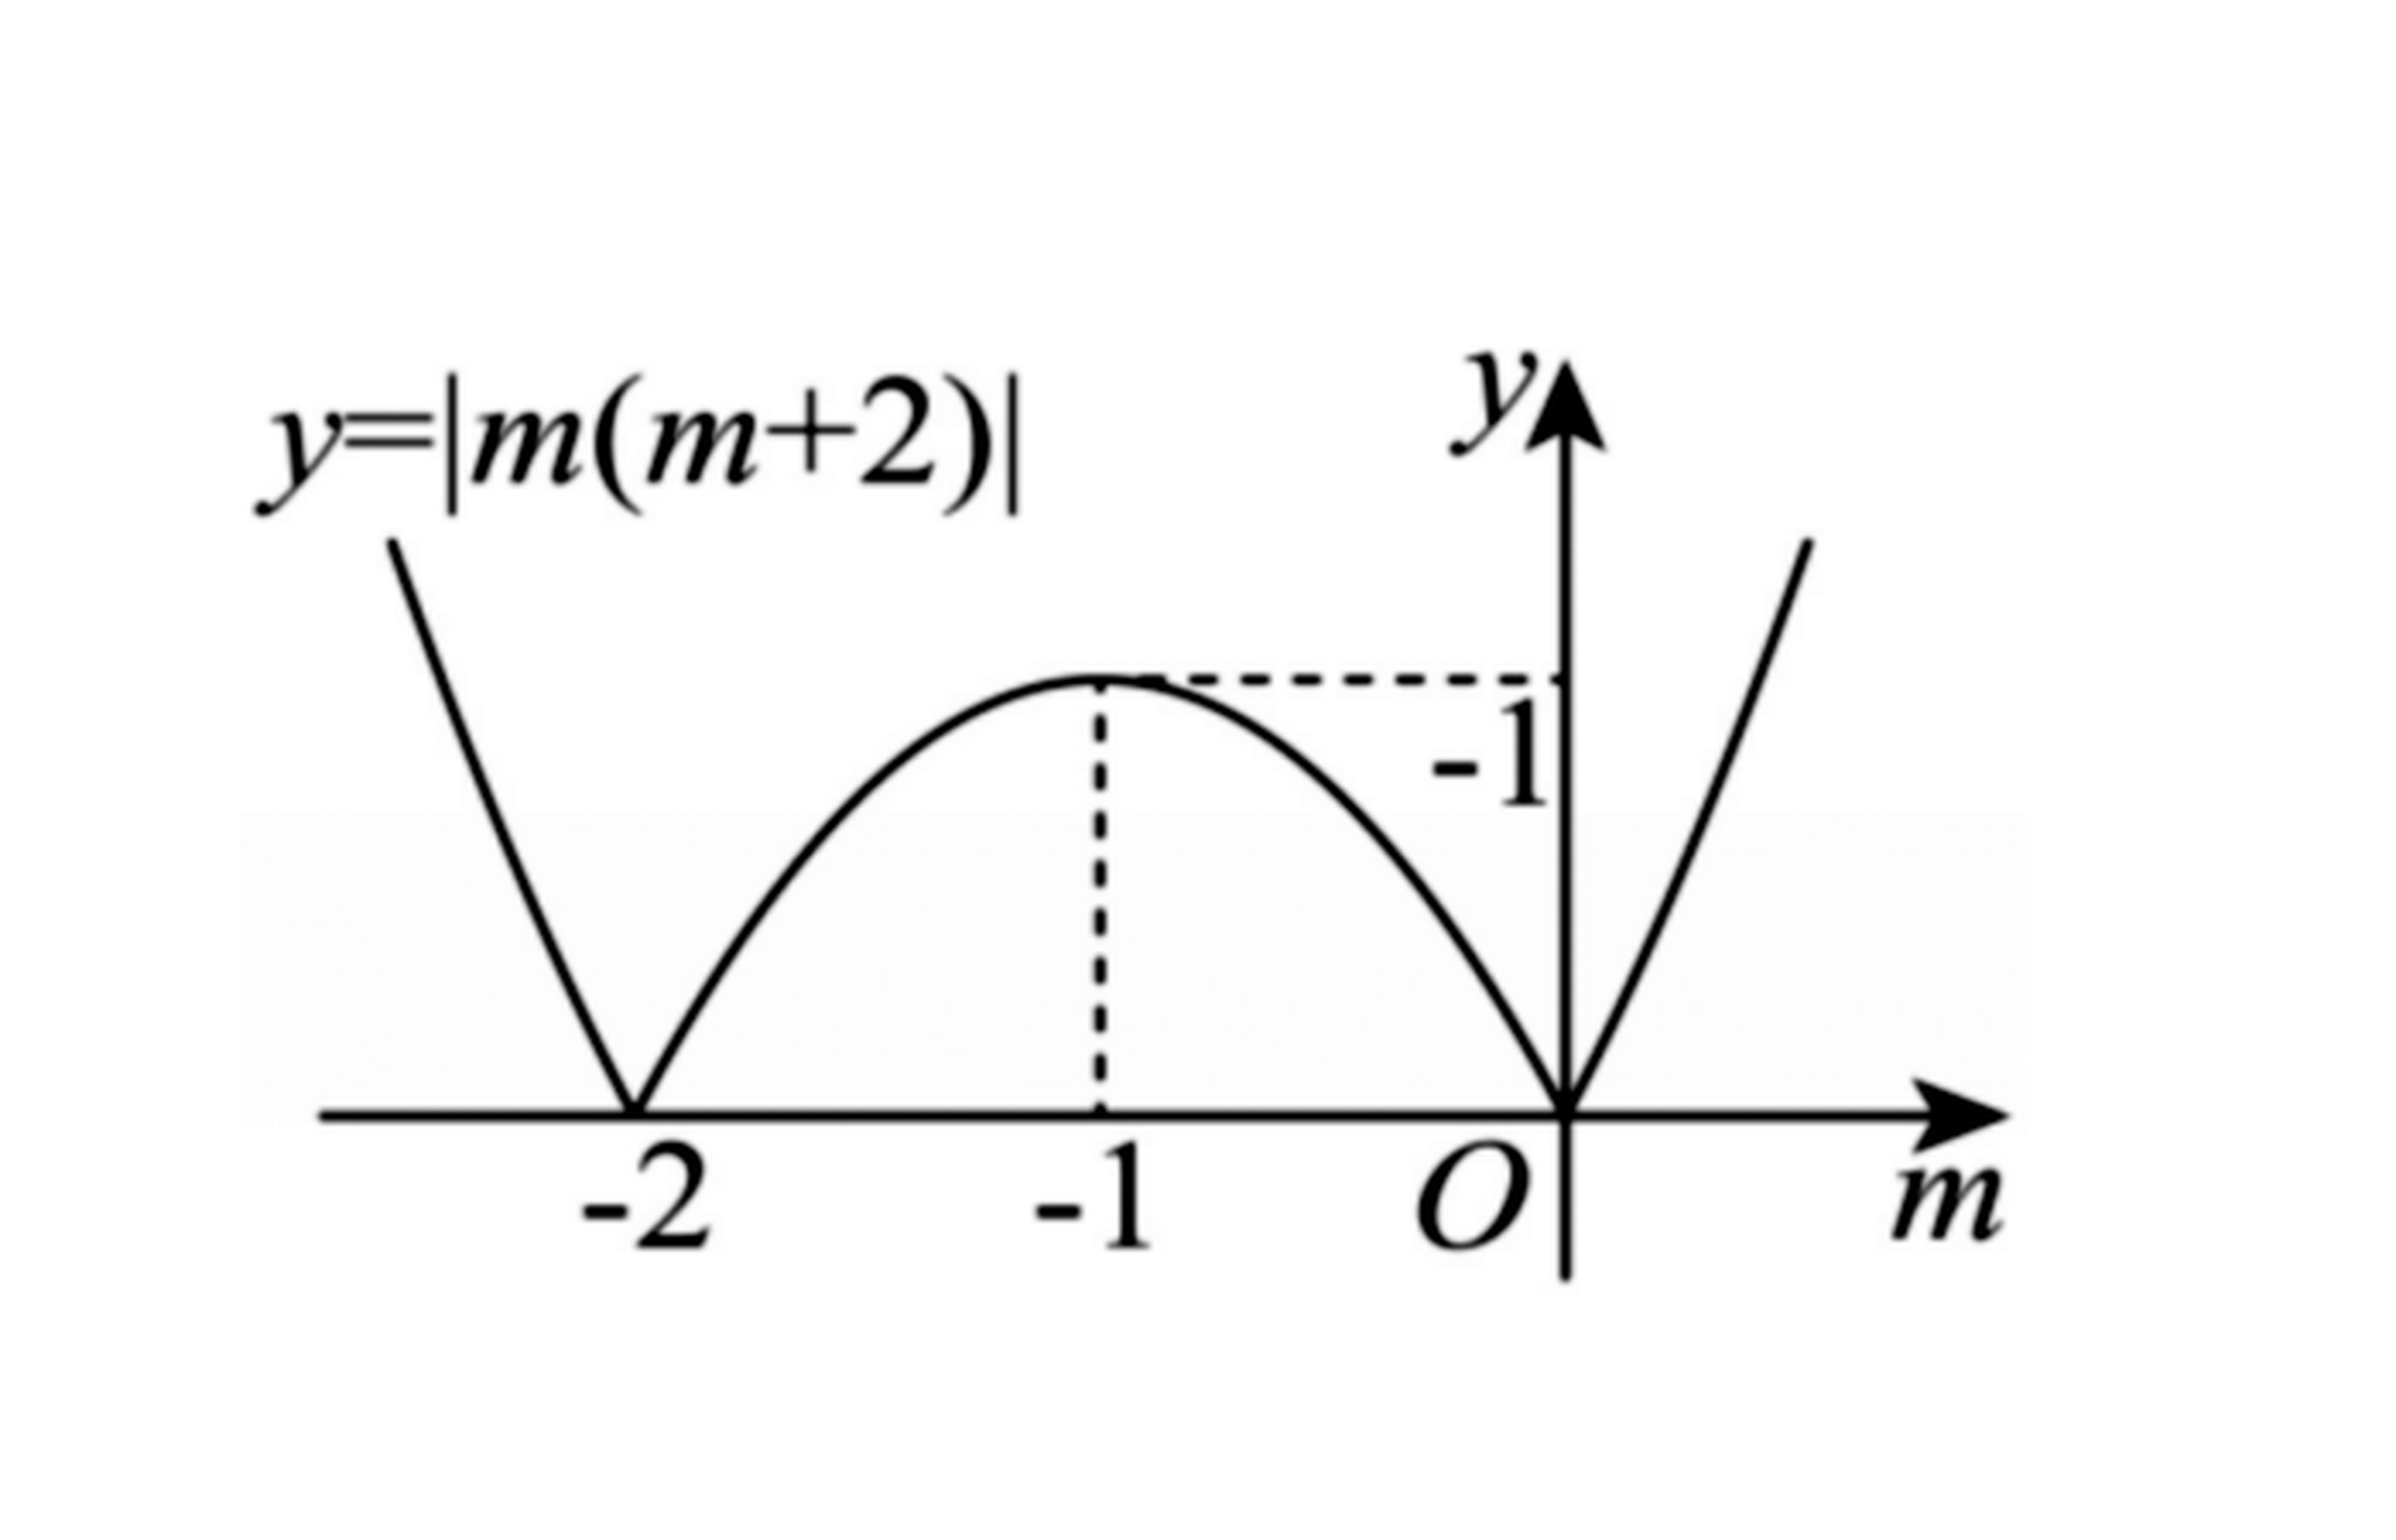
\includegraphics[width=0.46\textwidth]{figures/gao154_fujia2.png}
\end{center}
\step{由图像得 $k\in(0,1)$，}
\step{所以方程 $m^2+2m=k$ 和 $m^2+2m=-k$ 各有两个不同的根，}
\step{其中方程 $m^2+2m-k=0$ 的两根为 $m=-1\pm\sqrt{1+k}$，}
\step{方程 $m^2+2m+k=0$ 的两根为 $m=-1\pm\sqrt{1-k}$，}
\step{所以 $m_1=-1-\sqrt{1+k}$，$m_2=-1-\sqrt{1-k}$，$m_3=-1+\sqrt{1-k}$，$m_4=-1+\sqrt{1+k}$，且 $m_1<m_2<m_3<m_4$，}
\step{由 $m=\log_2 x$，则 $x=2^m$，}
\step{所以 $a=2^{-1-\sqrt{1+k}}$，$b=2^{-1-\sqrt{1-k}}$，$c=2^{-1+\sqrt{1-k}}$，$d=2^{-1+\sqrt{1+k}}$，}
\step{所以 $ad=2^{-1-\sqrt{1+k}}\times2^{-1+\sqrt{1+k}}=2^{(-1-\sqrt{1+k})+(-1+\sqrt{1+k})}=2^{-2}=\dfrac14$，}
\step{$b+c=2^{-1-\sqrt{1-k}}+2^{-1+\sqrt{1-k}}=\dfrac{2^{-\sqrt{1-k}}+2^{\sqrt{1-k}}}{2}$，}
\step{令 $s=\sqrt{1-k}$，其中 $s\in(0,1)$，则 $b+c=\dfrac12\left(2^{-s}+2^s\right)$，}
\step{设函数 $y=2^s+\dfrac1{2^s}$，令 $r=2^s\in(1,2)$，所以 $y=r+\dfrac1r$ 在 $(1,2)$ 上严格增，}
\step{所以函数 $y=2^s+\dfrac1{2^s}$ 在 $(0,1)$ 上严格增，所以 $y=2^s+\dfrac1{2^s}\in\left(2,\dfrac52\right)$，}
\step{所以 $b+c=\dfrac{2^{-s}+2^s}{2}\in\left(1,\dfrac54\right)$，$ad(b+c)=\dfrac{b+c}{4}\in\left(\dfrac14,\dfrac5{16}\right)$，}
\step{所以 $ad(b+c)$ 的取值范围是 $\left(\dfrac14,\dfrac5{16}\right)$，故选 $A$.}
\solend
\fi

\end{enumerate}

\end{document}
"
%
% ① 原始材料：微信公众号"魔都数学加油站"文章，连载"27学年高一154"，原文标题
% "27学年高一154——2026-2027年上海市徐汇中学高一上期中"；
% 原文链接：https://mp.weixin.qq.com/s/Qs2T7Zwsug-KKFE2wefDUg 。
% 正文为 12 张 PNG 页（01/03/04/05/07/11/12 为 2560×3620，
% 02/06/08/09/10 为 4762×6735，同一篇各页分辨率混排，逐页按各自分辨率裁图核对）。
% 体例：讲评版——一、填空题 3—12（10 题）、二、选择题 13—16（4 题）、
% 三、解答题 17—21（5 题）、附加题 1—2（2 题，原卷**另起编号**"1." "2."，
% 不与正题连号，同 高一a 成例），共 21 题；全卷每题均印【解析】
% （逐题核实，见 ② ②）。题目、答案、解析均据原图转录；卷面粉红色水印
% "魔都数学加油站"及公众号页脚未录入。
% 全卷插图清单（逐页通读 12 页确认）：3 组——
%   · Q15 题干配图（$f(x)=(x-a)(x-b)$ 抛物线，04 页右下：x/y 轴、O、1、
%     开口向上两零点均在 (0,1) 内），三版都出，裁 figures/gao154_q15_stem.png；
%   · Q15 四幅图像选项（05 页上半 2×2 排布，A/B/C/D 四幅指数函数图像，
%     合并成一张，照 高一136 Q13/Q22 成例），三版都出，
%     裁 figures/gao154_q15_opts.png；
%   · 附加题第 2 题解析配图（$y=\lvert m(m+2)\rvert$ 图像，11 页右上：
%     W 形折线、$-2$、$-1$、O、虚线 $y=1$ 与 $m=-1$），仅答案版出，
%     裁 figures/gao154_fujia2.png；
%   3 图均取自原卷截图，去粉色水印、去色、4× LANCZOS 放大；Q15 题干图
%   左侧题干残字"的图"已裁白。其余各页逐页确认无其它题目配图、无表格；
%   12 页下半仅水印、无正文。
%
% 卷首标题：原卷印作"2026-2027 年徐汇中学高一上期中"，年份区间按全稿惯例排 en dash；
% 原卷卷面未印副标题，本稿按同期中卷知识模块口径补出"集合与常用逻辑用语、不等式、函数"。
%
% ② 与原卷的排版差异：
%   ① 原文从第 3 题起，本稿保留原题号；共 21 题四节，正题到 21，附加题另起编号
%      1—2（\bigsec{附加题} 后 \begin{enumerate} 不 \setcounter，同 高一a 成例）；
%   ② 全 21 题均印【解析】、用 \solbegin…\solend，无只印【答案】或答案印括号内的题；
%      四道正题选择题答案在解析末句"故选 C／A／B／C"（Q13—Q16）、附加题第 2 题
%      答案在解析末句"故选 A"，括号 \mbox{（\quad）} 留空、不另提 \ans{}；
%      答案版【答案】/【解析】标记数 = 21 = 全卷题数；
%   ③ 原卷卷面未印副标题，本稿按知识模块口径补出；
%   ④ 原卷填空横线按全稿惯例排 \blankline[4.4em]；选择题括号排 \mbox{（\quad）}、
%      四道正题选择题与附加题第 2 题的选项段前按惯例各加 \keepwithprev
%      （Q15 与附加题 2 的选项段是整块图，\keepwithprev 后接 \begin{center}）；
%      解答题不留作答区、不加 \anspace（原卷为讲评版）；
%   ⑤ 数集黑板粗体：Q4"$x,y\in R$"、Q9"$x\in\R$"、Q13 无、
%      Q15"定义域 $\R$"、Q19"$\forall x\in\R$"、Q21"$x\in\N$"与"$k\in\N^*$"、
%      Q20"$a,b\in\R$"、附加题 2 无——原卷印斜体或正体粗体 R/N/N*，
%      按全稿惯例归一 \R／\N／\N^*；绝对值排 \lvert…\rvert
%      （Q5、Q9、Q12、Q13、Q16、Q21、附加题 2），集合描述竖线排 \mid
%      （Q5、Q17、Q19、Q21），不等号按全稿惯例排 \leqslant／\geqslant；
%      空集 \varnothing（Q21 题干 (3)）；
%   ⑥ 子集符号逐处照录、不得统一：Q6 题干印"$\{1,2\}\subset M\subseteq\{1,2,3,4,5\}$"
%      （前单线 ⊂、后带下划线 ⊆，同句两形并用），解析亦两形并用；
%      Q17 解析 (2)"$B\subset A$"印单线 ⊂；Q21 题干 (3)"$A\subseteq\{x\mid\cdots\}$"
%      印带下划线 ⊆——逐处放大核，分别 \subset／\subseteq，照录未统一（见 ④）；
%   ⑦ 判别式 Δ/△：Q18 解析 (1)"$\Delta=m^2-4(4m^2-3)$"与 Q19 解析 (1)
%      "$\Delta=4m^2-8m<0$"两处均印等腰偏高粗三角、照录 \Delta；本卷无扁等边
%      细线 \triangle 用例（见 ④）；
%   ⑧ 中文弯引号照录：Q4"设 $x$、$y\in\R$. 若 $x+y>2$，则 $x>1$ 或 $y>1$"、
%      附加题 1"$n$ 元集和集"与"3 元集和集"；注释里一律 ASCII 引号；
%      数学式内 CJK 用 \text{}（Q5 解集描述"或"、Q19 集合描述的"或"）；
%   ⑨ "图像／图象"逐处放大核：Q15 题干与解析印"图象"（象，无亻）、
%      Q16 无、附加题 2 解析印"图象"与"图像"（"画出函数…的图象"、
%      "由图像得"——两形并用，逐处照录未统一）；Q13/Q14 无数集图像字样；
%      半角逗号在数学组之间是全稿惯例、非笔误，逐处照录（Q3、Q10、Q16、
%      Q18、Q20、Q21 的 $x_1,x_2$ 之类）；行末西文句点 ASCII `.`；
%      行中全角逗号／顿号照录（Q6"3，4，5"、Q20"（单位：元）"、
%      附加题 1"$a_1,a_2,a_3,a_4$"）；
%   ⑩ 复杂式照录别简化：Q3 $a^{\frac{12}{7}}\cdot\left(\frac17\right)^{\frac17}
%      \cdot\sqrt[7]{a^4}$ 与 $7^{-\frac17}a^{\frac{16}{7}}$、Q7 $x^{-m}$、
%      Q8 $\frac{b-2a+2}{2a}$、Q11 $\frac{9+4\sqrt2}{6}$、Q12 $506\frac29$ 与
%      $506\frac49$、Q16 高斯取整 $[a]$、Q20 $c(x)=10x+\frac1{100}x^2$ 与
%      $q(x)=a+\frac xb$、Q21 $A^+$／$A^-$ 与 $|A^+|\geqslant2k-1$、
%      附加题 2 $m=-1\pm\sqrt{1+k}$ 与 $ad(b+c)$；
%      \left…\right 不得拆到不同 $…$ 组（Q5 $\left\{x\mid\cdots\right\}$、
%      Q20 $\left(\frac1b-\frac1{100}\right)$、附加题 2 $\left(\frac14,\frac5{16}\right)$）；
%      cases 块一律 \begin{cases}…\end{cases}；
%   ⑪ 一条 \step = 原卷解析的一个印刷行，cases 块整体算一个印刷行；别并折行、
%      别拆行。Q11 九行、Q12 六行、Q16 十六行、Q20 十一行、Q21 十七行、
%      附加题 2 十八行均按印刷行逐条断，不丢行；
%   ⑫ 配图：Q15 题干小图（三版都出）放 \item 内题干之后 \begin{center}，
%      Q15 四幅选项图（三版都出）放 \keepwithprev 之后的 \begin{center}，
%      Q15 用 \needvspace 守卫把"题干＋两图"整块推走（守卫放 \item 之前，
%      见 高一145 Q14/Q20 与 高一136 Q13 成例）；附加题 2 解析配图（仅答案版出）
%      放 \ifanswer 内 \solbegin…\solend 的 \step 之间（高一73 第 16 题成例）；
%   ⑬ 原卷解析内无红色"法一／法二"之类小标题，故本卷无 \stepm；红色水印
%      "魔都数学加油站"不录入；
%   ⑭ 跨页续印按题合并：见 ⑥；
%
% ③ 行数复核：一条 \step = 原卷解析的一个印刷行，cases 块作一个印刷行计。
%   逐题数（主会话逐页核对定稿）：Q3：1；Q4：1；Q5：3；Q6：4；Q7：3；
%   Q8：1；Q9：5；Q10：4；Q11：9；Q12：6；Q13：5；Q14：4；Q15：3；
%   Q16：16；Q17：5；Q18：9；Q19：10；Q20：11；Q21：17；
%   附加题 1：6；附加题 2：18。
%   合计 141 条 \step（本卷无 \stepm），与原卷逐题印刷行相等。全卷 21 题
%   均设 \solbegin…\solend，答案版【答案】/【解析】标记数 = 21 = 全卷题数。
%
% ④ 判别式／子集符号结论（逐处放大原图照录、不得统一，主会话像素级复核）：
%   判别式：Q18 解析 (1)"$\Delta=m^2-4(4m^2-3)=-15m^2+12\geqslant0$"、
%      Q19 解析 (1)"$\Delta=4m^2-8m<0$"共 2 处，逐处放大确认印等腰偏高
%      粗三角（高>宽、右斜边粗），照录 \Delta；本卷无扁等边细线 \triangle
%      用例，无几何三角形符号。
%   子集：Q6 题干"$\{1,2\}\subset M\subseteq\{1,2,3,4,5\}$"前 ⊂ 单线、
%      后 ⊆ 带下划线（/tmp/gao154/z/zoom/q6_subset.png），解析两处同样两形
%      并用，分别照录 \subset／\subseteq；Q17 解析 (2)"$B\subset A$"单线
%      照录 \subset；Q21 题干 (3)"$A\subseteq\{x\mid\cdots\}$"带下划线
%      照录 \subseteq。本卷 ⊂ 与 ⊆ 混用逐处照录、不得统一。
%      空集 \varnothing（Q21 题干 (3)）、数集 \R／\N／\N^* 归一见 ② ⑤。
%
% ⑤ 存疑照录（放大原图确认，照录未改、正文对应处另有 % 注）：
%   1. Q7 题干印 $f(x)=(3m-1)x^{-m}$，解析首句却写"幂函数 $f(x)=x^\alpha$
%      的系数必须为 1"（用 $\alpha$ 作指数记号），随后 $f(2)=2^\alpha=8$
%      得 $\alpha=3$、$f(x)=x^3$——题干指数 $-m$ 与解析 $\alpha$ 记法不同，
%      系原卷记号前后不一，逐处照录未统一（放大 01/02 页确认）。
%   2. Q11 解析"因为 $u>0,v>0$，由基本不等式得 $\frac{4v}{u}+\frac{2u}{v}
%      \geqslant2\sqrt{\frac{4v}{u}\cdot\frac{2u}{v}}=4\sqrt2$"与
%      "所以 $\frac4u+\frac1v=\frac16\left(\frac4u+\frac1v\right)(2u+v)$"
%      照录，未把 $u,v$ 化简回 $x,y$。
%   3. Q16 解析把"$[a]$ 表示不超过 $a$ 的最大整数"与"和至少有一个不小于 2"
%      连写在同一行（原卷如此），照录未改；末行"假设成立，C 正确，D 错误"照录。
%   4. Q18 解析 (2)"函数 $y=-7m^2+6$ 开口向下，对称轴为 $m=0$"却称求
%      "$y_{\min}$"（实为在 $m^2\leqslant\frac45$ 闭区间上的最小值），
%      照录未改。
%   5. Q20 题干"$q(x)=a+\frac xb$（$a,b\in\R$）"与解析
%      "$W(x)=\left(\frac1b-\frac1{100}\right)x^2+(a-10)x-160000$"照录；
%      末行解得 $a=90,b=\frac{500}{3}$ 照录未化简。
%   6. Q21 题干 (3)"$A\subseteq\{x\mid0\leqslant x\leqslant2020,x\in\N\}$"
%      与解析"$3k-1\leqslant2a_k+1\leqslant4041$（$k\in\N^*$）"照录；
%      末行"集合 $A$ 中元素的个数的最大值是 1347"照录。
%   7. 附加题 1 解析"相加化简得 $a_1+a_2+a_3+a_4=5$"照录；
%      附加题 2 解析"由图像得 $k\in(0,1)$"与"由图像得"／"的图象"两形
%      并用逐处照录（见 ② ⑨）；末行"$ad(b+c)$ 的取值范围是
%      $\left(\frac14,\frac5{16}\right)$，故选 A"照录。
%   全卷除此 7 类外未发现其它笔误／自相矛盾处；21 题均印【解析】、
%   无只印【答案】或答案印括号内的题（见 ② ②）。
%
% ⑥ 跨页续印按题合并说明（逐页核实定稿）：Q3—Q5 题干＋解析在 01 页
%   （Q5 解析末 2 行续 01 页下半）；Q6、Q7 题干＋解析在 01 页下半
%   （Q7 解析余 2 行续 02 页顶）；Q8、Q9 题干＋解析在 02 页上半
%   （Q9 解析余 3 行续 02 页下半）；Q10 题干＋解析在 02 页下半；
%   Q11 题干＋解析前 6 行在 03 页上半、余 3 行续 03 页下半；
%   Q12 题干＋解析前 5 行在 03 页下半、末行续 04 页顶；"二、选择题"
%   标题与 Q13 题干＋选项＋解析在 04 页上半；Q14 题干＋选项＋解析、
%   Q15 题干＋题干配图在 04 页下半；Q15 四幅选项图＋解析、
%   Q16 题干＋选项＋解析首行在 05 页上半，Q16 解析余 12 行在
%   05 页下半—06 页上半；"三、解答题"标题与 Q17 题干＋两问＋解析
%   在 06 页下半；Q18 题干＋两问＋解析在 07 页上半—下半；
%   Q19 题干＋两问＋解析首行在 07 页下半，解析余 8 行在 08 页上半；
%   Q20 题干在 08 页下半，解析 (1) 4 行＋(2) 首 4 行在 08 页下半—09 页上半，
%   (2) 余 2 行在 09 页下半；Q21 题干＋三问＋解析 (1)(2) 4 行在
%   09 页下半—10 页上半，解析 (3) 余 12 行在 10 页上半—下半；
%   "附加题"标题与附加题 1 题干＋解析首 3 行在 10 页下半，
%   余 3 行续 11 页上半；附加题 2 题干＋选项＋解析前 3 行在 11 页上半，
%   解析配图＋余 12 行在 11 页下半—12 页上半，末行
%   "所以 $ad(b+c)$ 的取值范围是 $\left(\frac14,\frac5{16}\right)$，故选 A"
%   为全卷收尾（12 页下半仅水印、无正文）。
%   本稿按题连排，不丢行、不并折行；全卷末题为附加题第 2 题。
%
\documentclass[a4paper,11pt]{article}
\usepackage{common}

\begin{document}

\examtitlest[3]{2026--2027 年徐汇中学高一上期中}{集合与常用逻辑用语、不等式、函数}

\bigsec{一、填空题}

\begin{enumerate}
\setcounter{enumi}{2}

% === Q3 === 分数指数幂照录；解析 1 行
\item 已知 $a>0$，化简 $a^{\frac{12}{7}}\cdot\left(\dfrac17\right)^{\frac17}\cdot\sqrt[7]{a^4}=$\blankline[4.4em].

\ifanswer
\solbegin
\step{$a^{\frac{12}{7}}\cdot\left(\dfrac17\right)^{\frac17}\cdot\sqrt[7]{a^4}=a^{\frac{12}{7}}\cdot(7^{-1})^{\frac17}\cdot a^{\frac47}=7^{-\frac17}a^{\frac{16}{7}}$.}
\solend
\fi

% === Q4 === 反证法；中文弯引号照录；解析 1 行
\item 用反证法证明命题：“设 $x$、$y\in\R$. 若 $x+y>2$，则 $x>1$ 或 $y>1$”时，假设的内容应该是\blankline[4.4em].

\ifanswer
\solbegin
\step{由反证法得，假设的内容应该是 $x\leqslant1$ 且 $y\leqslant1$.}
\solend
\fi

% === Q5 === 分式不等式；cases 块；解析 3 行
\item 不等式 $\dfrac{2x+3}{x-1}\geqslant1$ 的解集为\blankline[4.4em].

\ifanswer
\solbegin
\step{$\dfrac{2x+3}{x-1}\geqslant1$，即 $\dfrac{2x+3}{x-1}-1\geqslant0$，$\dfrac{x+4}{x-1}\geqslant0$，}
\step{等价于 $\begin{cases}(x+4)(x-1)\geqslant0\\x-1\ne0\end{cases}$，解得 $x>1$ 或 $x\leqslant-4$，}
\step{故解集为 $\{x\mid x>1\text{ 或 }x\leqslant-4\}$.}
\solend
\fi

% === Q6 === ⊂ 与 ⊆ 并用照录；解析 4 行
\item 满足条件 $\{1,2\}\subset M\subseteq\{1,2,3,4,5\}$ 的集合 $M$ 的个数为\blankline[4.4em].

\ifanswer
\solbegin
\step{因为 $\{1,2\}\subset M\subseteq\{1,2,3,4,5\}$，所以集合 $M$ 必含有元素 1，2，}
\step{且至少含有元素 3，4，5 中的一个，}
\step{则集合 $M$ 的个数与集合 $\{3,4,5\}$ 的非空子集的个数一样，}
\step{所以集合 $M$ 的个数为 $2^3-1=7$.}
\solend
\fi

% === Q7 === 题干 $x^{-m}$、解析用 $x^\alpha$ 记法，原卷记号差异照录（见 ⑤ 1）；解析 3 行
\item 已知幂函数 $f(x)=(3m-1)x^{-m}$，且 $f(2)=8$，则 $f(m)=$\blankline[4.4em].

\ifanswer
\solbegin
\step{幂函数 $f(x)=x^\alpha$ 的系数必须为 1，所以 $3m-1=1$，得 $m=\dfrac23$.}
\step{又 $f(2)=2^\alpha=8=2^3$，故 $\alpha=3$，即 $f(x)=x^3$，}
\step{所以 $f(m)=f\left(\dfrac23\right)=\left(\dfrac23\right)^3=\dfrac8{27}$.}
\solend
\fi

% === Q8 === 换底公式；解析 1 行
\item 已知 $a=\lg2$，$b=\lg3$，用含 $a,b$ 的代数式表示 $\log_4 75=$\blankline[4.4em].

\ifanswer
\solbegin
\step{$\log_4 75=\dfrac{\lg\left(3\times\frac{10^2}{2^2}\right)}{\lg2^2}=\dfrac{\lg3+2-2\lg2}{2\lg2}=\dfrac{b-2a+2}{2a}$.}
\solend
\fi

% === Q9 === 三角不等式取等；解析 5 行
\item 设 $x\in\R$，则方程 $\lvert x-2\rvert+\lvert3x+1\rvert=\lvert2x+3\rvert$ 的解集是\blankline[4.4em].

\ifanswer
\solbegin
\step{由 $\lvert x-2\rvert=\lvert2-x\rvert$，故原方程可化为 $\lvert2-x\rvert+\lvert3x+1\rvert=\lvert2x+3\rvert$，}
\step{又 $(2-x)+(3x+1)=2x+3$，}
\step{由三角不等式 $\lvert2-x\rvert+\lvert3x+1\rvert\geqslant\lvert(2-x)+(3x+1)\rvert=\lvert2x+3\rvert$，}
\step{当且仅当 $(2-x)(3x+1)\geqslant0$ 等号成立，}
\step{解 $(2-x)(3x+1)\geqslant0$ 得 $-\dfrac13\leqslant x\leqslant2$，故原方程的解集为 $\left[-\dfrac13,2\right]$.}
\solend
\fi

% === Q10 === 韦达定理；cases 块；解析 4 行
\item 已知一元二次不等式 $x^2+bx+c>0$ 的解集为 $(-\infty,-1)\cup(2,+\infty)$，则一元二次不等式 $bx^2+cx-1<0$ 的解集是\blankline[4.4em].

\ifanswer
\solbegin
\step{因为 $x^2+bx+c>0$ 的解集为 $(-\infty,-1)\cup(2,+\infty)$，}
\step{所以方程 $x^2+bx+c=0$ 的两根为 $-1$ 和 2，则有 $\begin{cases}-b=-1+2\\c=-1\times2\end{cases}$，即 $\begin{cases}b=-1\\c=-2\end{cases}$，}
\step{则 $bx^2+cx-1<0$ 等价于 $-x^2-2x-1<0$，得 $x^2+2x+1>0$，得 $(x+1)^2>0$，}
\step{解得 $x\ne-1$，故不等式 $bx^2+cx-1<0$ 的解集为 $(-\infty,-1)\cup(-1,+\infty)$.}
\solend
\fi

% === Q11 === 换元 $u,v$；解析 9 行
\item 已知正数 $x,y$ 满足 $2x+y=1$，则 $\dfrac4{x+2}+\dfrac1{y+1}$ 的最小值为\blankline[4.4em].

\ifanswer
\solbegin
\step{令 $u=x+2$，$v=y+1$，则 $u>2$，$v>1$，}
\step{且 $2u+v=2(x+2)+(y+1)=2x+y+5=6$.}
\step{因为 $u>0$，$v>0$，由基本不等式得 $\dfrac{4v}{u}+\dfrac{2u}{v}\geqslant2\sqrt{\dfrac{4v}{u}\cdot\dfrac{2u}{v}}=4\sqrt2$，}
\step{所以 $\dfrac4u+\dfrac1v=\dfrac16\left(\dfrac4u+\dfrac1v\right)(2u+v)=\dfrac16\left(9+\dfrac{4v}{u}+\dfrac{2u}{v}\right)\geqslant\dfrac{9+4\sqrt2}{6}$，}
\step{当且仅当 $\dfrac{4v}{u}=\dfrac{2u}{v}$，即 $u=\sqrt2v$ 时等号成立，}
\step{与 $2u+v=6$ 联立得 $u=\dfrac{6\sqrt2}{2\sqrt2+1}$，$v=\dfrac6{2\sqrt2+1}$，}
\step{此时 $x=u-2=\dfrac{2\sqrt2-2}{2\sqrt2+1}>0$，$y=v-1=\dfrac{5-2\sqrt2}{2\sqrt2+1}>0$，且 $2x+y=1$，}
\step{满足题设，所以下界可以取得，}
\step{因此 $\dfrac4{x+2}+\dfrac1{y+1}$ 的最小值为 $\dfrac{9+4\sqrt2}{6}$.}
\solend
\fi

% === Q12 === 2025 个整数解；解析 6 行
\item 若关于 $x$ 的不等式 $\lvert x-2k\rvert+\lvert x-3k\rvert<4k$ 共有 2025 个整数解，则实数 $k$ 的取值范围为\blankline[4.4em].

\ifanswer
\solbegin
\step{显然 $k>0$，由 $\lvert x-2k\rvert+\lvert x-3k\rvert<4k$，得 $\dfrac12k<x<\dfrac92k$，}
\step{因为该不等式共有 2025 个整数解，所以 $2024<\dfrac{9k}{2}-\dfrac k2\leqslant2026$，}
\step{解得 $506<k\leqslant506.5$，}
\step{由 $\dfrac k2\in(253,253.25]$，得这 2025 个整数解只能为 254、255、256、$\cdots$、2278，}
\step{所以 $2278<\dfrac{9k}{2}\leqslant2279$，解得 $506\dfrac29<k\leqslant506\dfrac49$，结合 $506<k\leqslant506.5$，}
\step{得 $k$ 的取值范围是 $\left(506\dfrac29,506\dfrac49\right]$.}
\solend
\fi

\end{enumerate}

\bigsec{二、选择题}

\begin{enumerate}
\setcounter{enumi}{12}

% === Q13 === 四选项一行；解析 5 行，故选 C
\item 若 $a<b<0$，则下列不等式中不成立的是\mbox{（\quad）}

\keepwithprev
A. $a-b>a$\qquad B. $\dfrac1a>\dfrac1b$\qquad C. $a^3>b^3$\qquad D. $\lvert a\rvert>\lvert b\rvert$

\ifanswer
\solbegin
\step{A 选项，因为 $b<0$，所以 $-b>0$，不等式两边同加上 $a$ 得 $a-b>a$，故 A 正确；}
\step{B 选项，因为 $a<b<0$，所以 $ab>0$，不等式两边同除以 $ab$，则 $\dfrac1b<\dfrac1a<0$，故 B 正确；}
\step{C 选项，不妨设 $a=-2$，$b=-1$，则 $a^3=-8$，$b^3=-1$，故 $a^3<b^3$，故 C 错误；}
\step{D 选项，因为 $a<b<0$，所以 $-a>-b$，即 $\lvert a\rvert>\lvert b\rvert$，故 D 正确.}
\step{故选 $C$.}
\solend
\fi

% === Q14 === 选项两行两列；解析 4 行，故选 A
\item 设命题 $p:x^2-5x+4\ne0$，命题 $q:x\ne1$，则 $p$ 是 $q$ 的\mbox{（\quad）}条件

\keepwithprev
A. 充分不必要\qquad\qquad B. 必要不充分

C. 充要\qquad\qquad D. 既不充分也不必要

\ifanswer
\solbegin
\step{$p:x^2-5x+4\ne0\Leftrightarrow(x-1)(x-4)\ne0\Leftrightarrow x\ne1$ 且 $x\ne4$；$q:x\ne1$.}
\step{充分性：当 $x\ne1$ 且 $x\ne4$ 时，$x\ne1$，所以 $p\Rightarrow q$；}
\step{必要性：当 $x\ne1$ 时，若 $x=4$，此时 $p$ 不成立，即 $q\nRightarrow p$；}
\step{所以 $p$ 是 $q$ 的充分不必要条件，故选 $A$.}
\solend
\fi

% === Q15 === 题干配图（三版都出）+ 四幅图像选项（2×2 合并，三版都出）；守卫放 \item 之前；解析 3 行，故选 B
\needvspace{9cm}
\item 已知函数 $f(x)=(x-a)(x-b)$（$a<b$）的图象如图所示，则函数 $g(x)=a^x-b$ 的图象可能是\mbox{（\quad）}

\begin{center}
% 抛物线题干配图取 04 页右下，去粉色水印、去色、4× LANCZOS 放大；三版都出
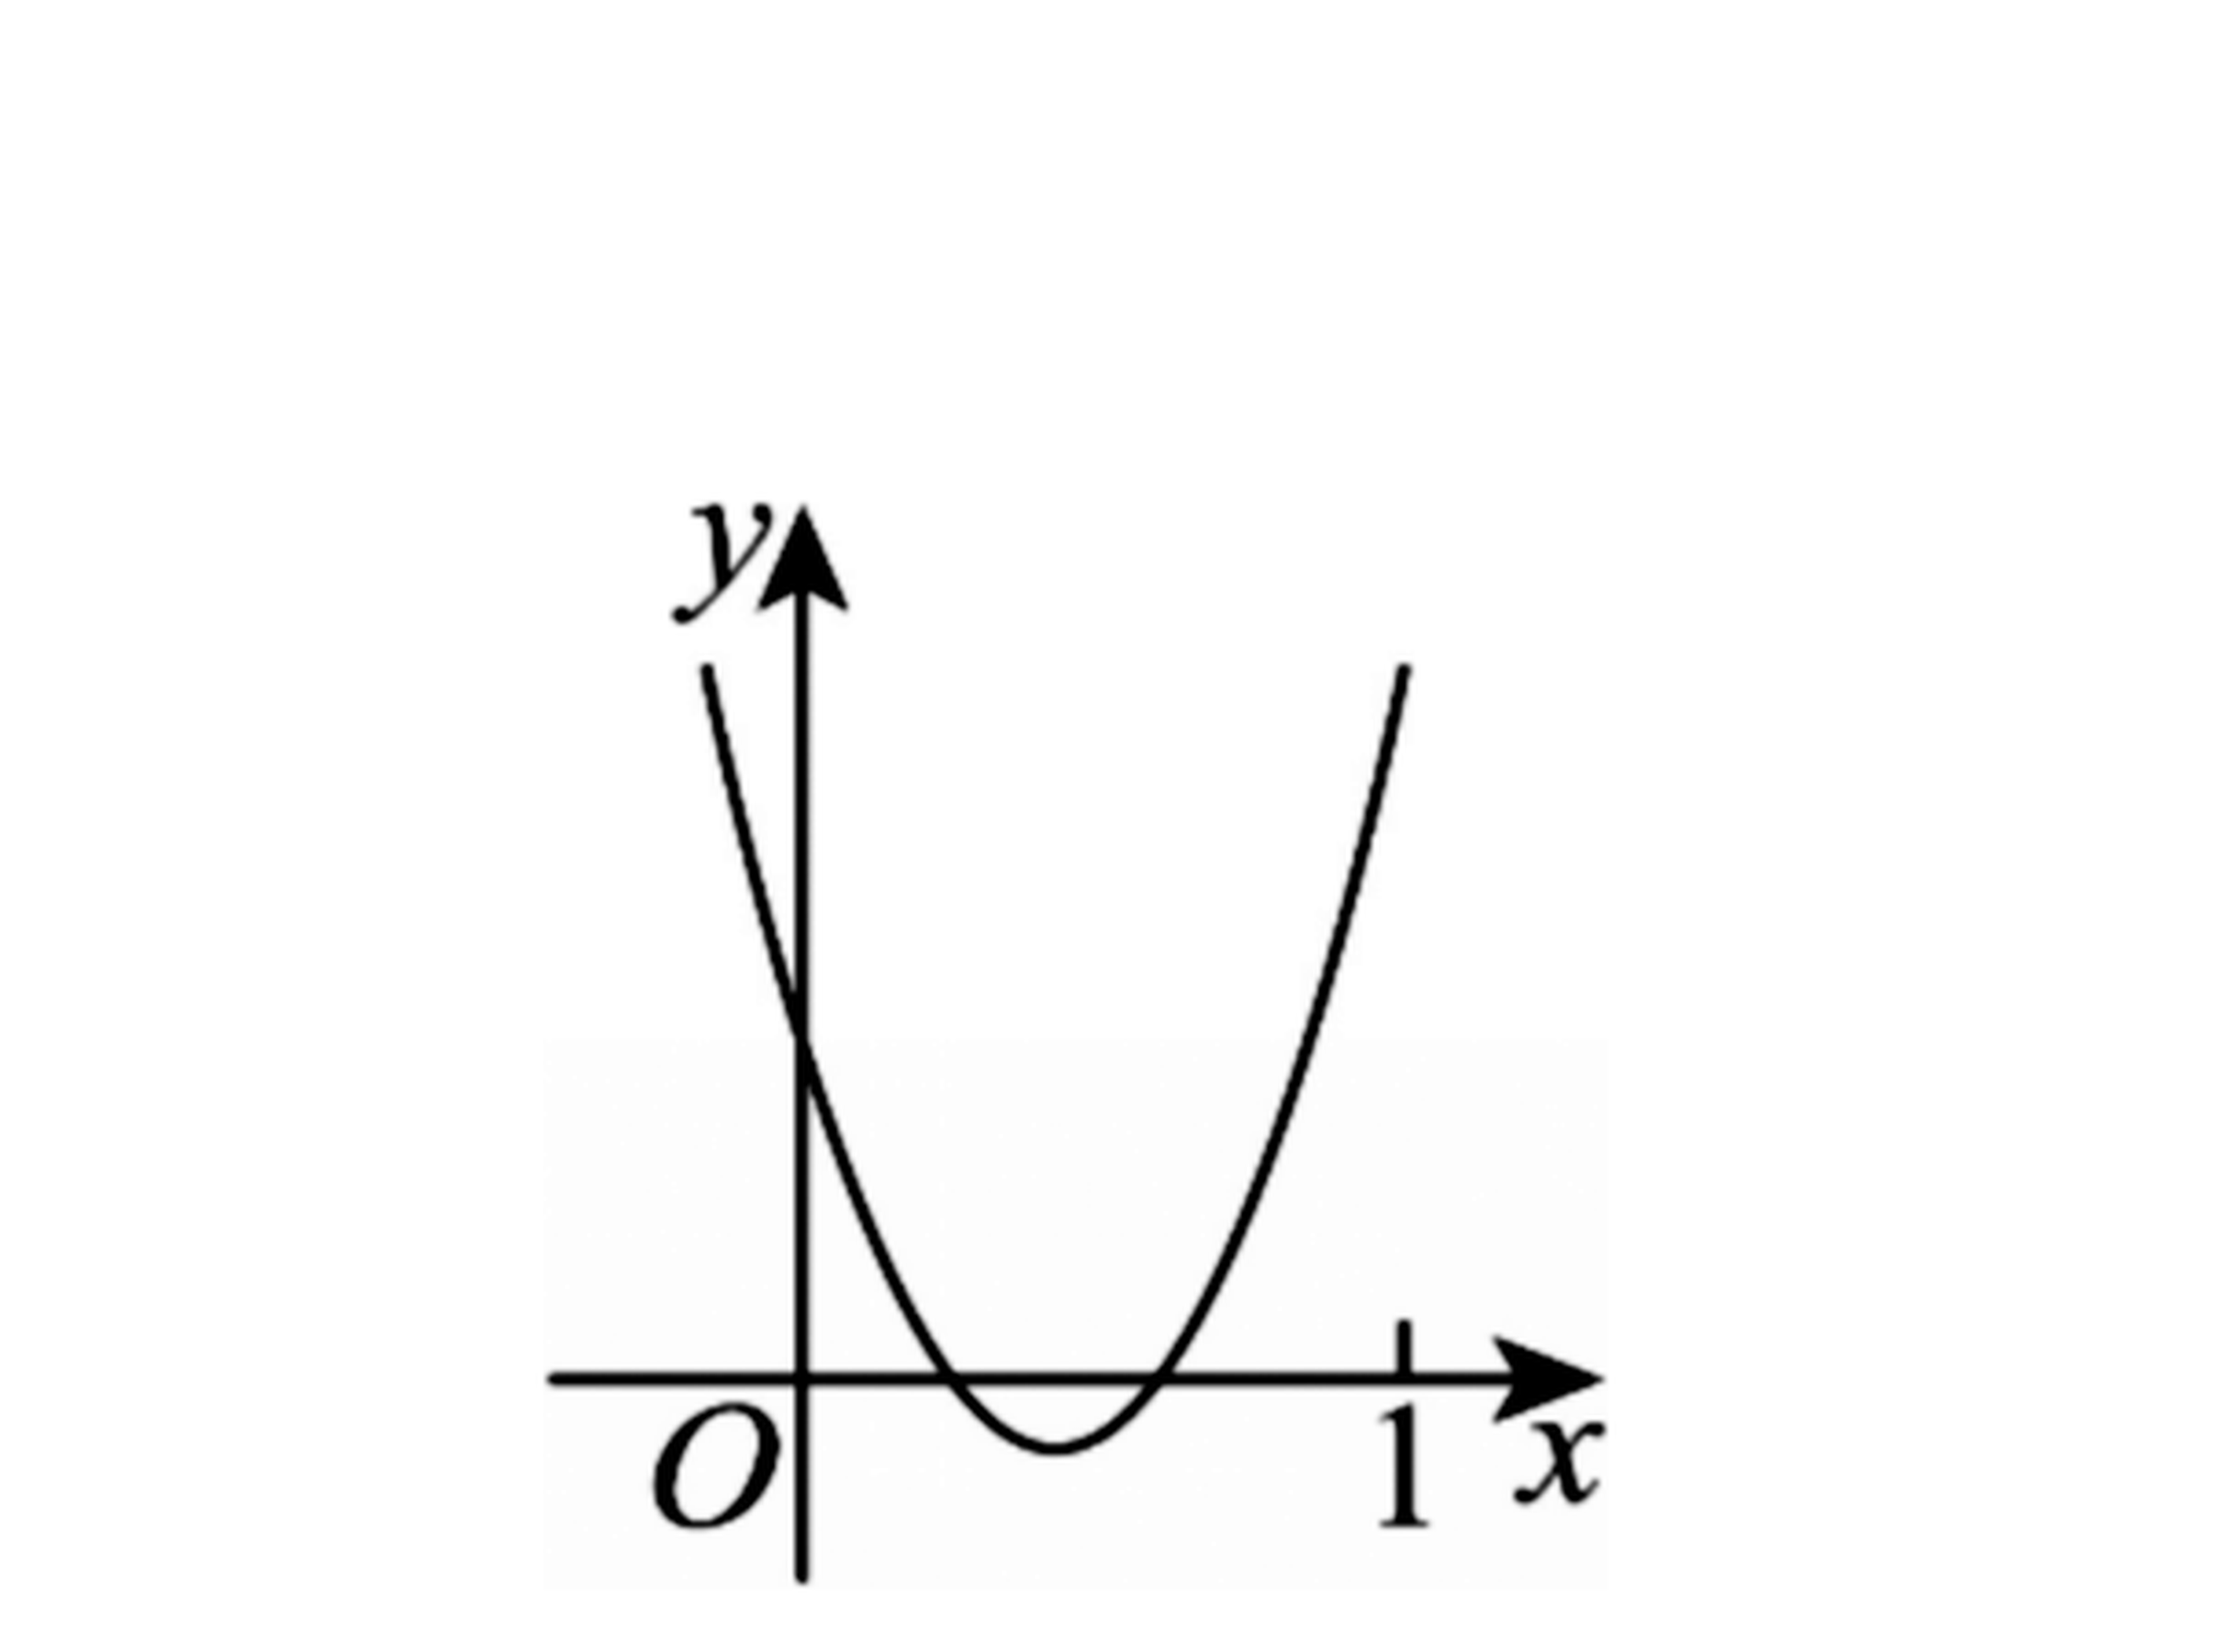
\includegraphics[width=0.32\textwidth]{figures/gao154_q15_stem.png}
\end{center}

\keepwithprev
\begin{center}
% 四幅指数函数图像选项取 05 页上半，按原卷 2×2 排布合并为一张，去粉色水印、去色、4× LANCZOS 放大；三版都出
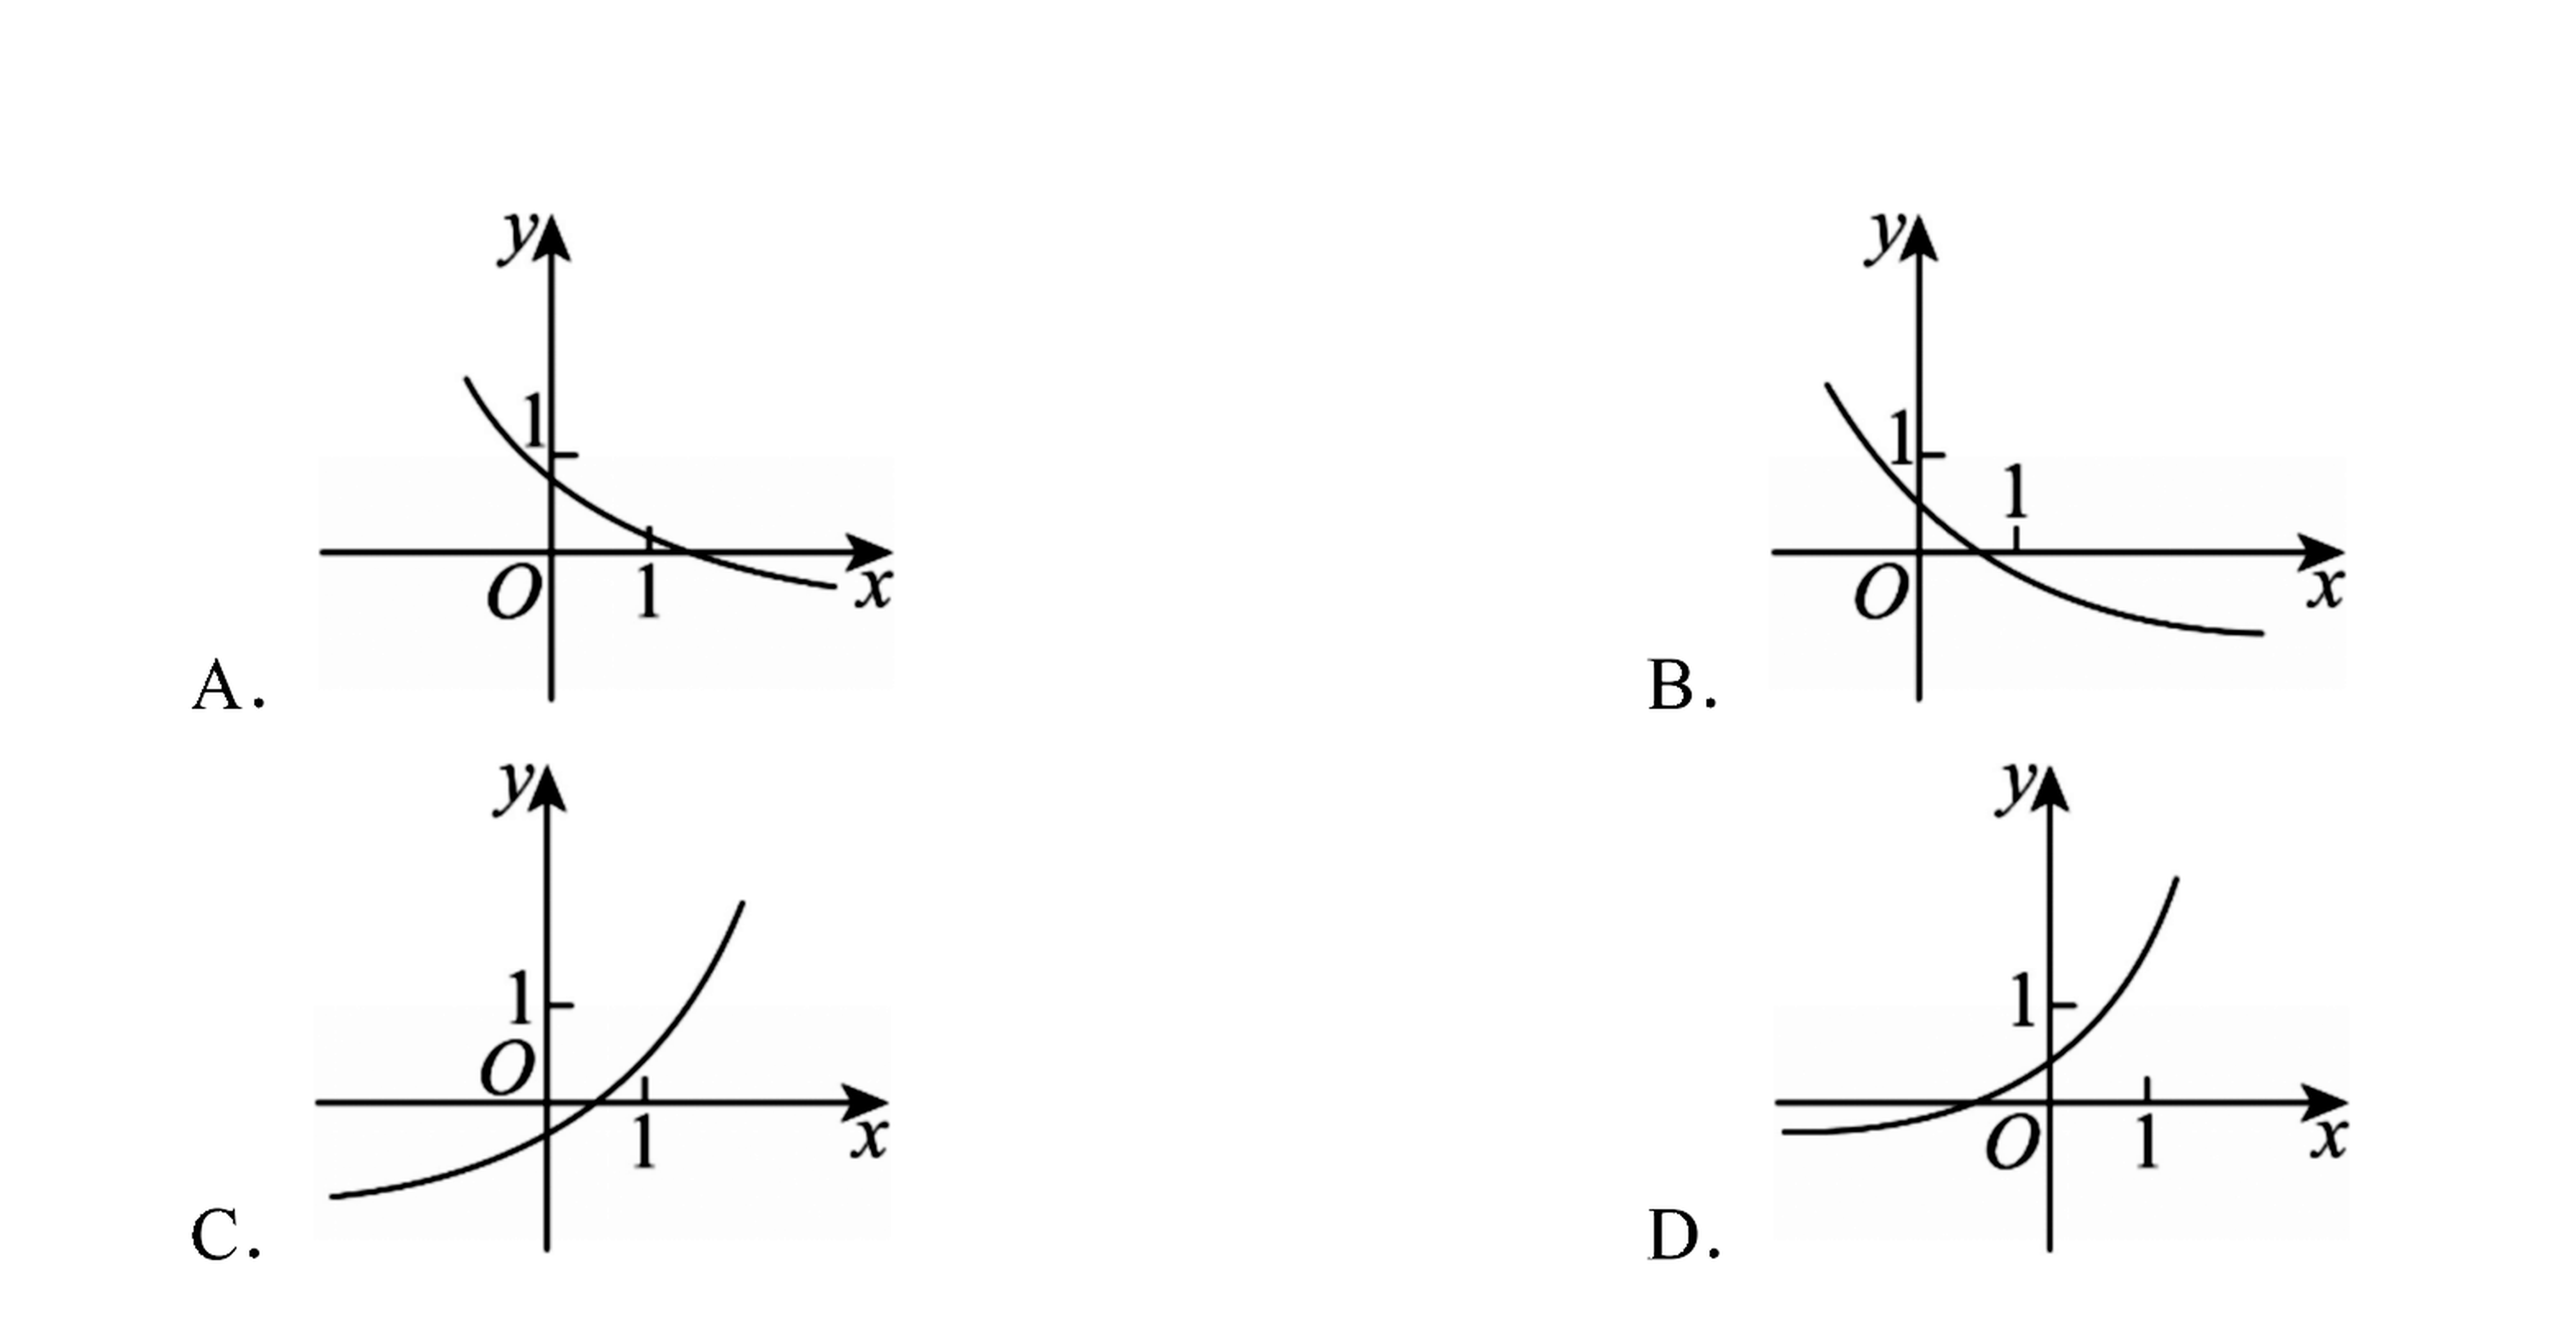
\includegraphics[width=0.80\textwidth]{figures/gao154_q15_opts.png}
\end{center}

\ifanswer
\solbegin
\step{由题意得 $0<a<b<1$，所以 $g(x)=a^x-b$ 在定义域 $\R$ 上严格减.}
\step{$g(0)=a^0-b=1-b>0$，$g(1)=a^1-b=a-b<0$，故 B 符合题意.}
\step{故选 $B$.}
\solend
\fi

% === Q16 === 高斯取整；解析 13 行，故选 C
\item 设 $[a]$ 表示不超过 $a$ 的最大整数，如 $[1.2]=1$，$[-3.2]=-4$，若 $x$、$y$、$z$ 为正实数，则 $\left[\dfrac{y+z}{x}\right]+\left[\dfrac{z+x}{y}\right]+\left[\dfrac{x+y}{z}\right]$ 的最小值为\mbox{（\quad）}

\keepwithprev
A. 2\qquad\qquad B. 3\qquad\qquad C. 4\qquad\qquad D. 6

\ifanswer
\solbegin
\step{若 $x$、$y$、$z$ 为正实数，}
\step{结合基本不等式得 $\dfrac{y+z}{x}+\dfrac{z+x}{y}+\dfrac{x+y}{z}=\dfrac yx+\dfrac xy+\dfrac zx+\dfrac xz+\dfrac zy+\dfrac yz$}
\step{$\geqslant2\sqrt{\dfrac yx\cdot\dfrac xy}+2\sqrt{\dfrac zx\cdot\dfrac xz}+2\sqrt{\dfrac zy\cdot\dfrac yz}=6$，当且仅当 $x=y=z$ 时取等号，}
\step{即 $\dfrac{y+z}{x}$，$\dfrac{z+x}{y}$，$\dfrac{x+y}{z}$ 中至少有一个不小于 2，不妨设 $\dfrac{y+z}{x}\geqslant\dfrac{z+x}{y}\geqslant\dfrac{x+y}{z}$，}
\step{$[a]$ 表示不超过 $a$ 的最大整数和 $\dfrac{y+z}{x}$，$\dfrac{z+x}{y}$，$\dfrac{x+y}{z}$ 中至少有一个不小于 2，}% 原卷此行把两句连写，照录未改（见 ⑤ 3）
\step{得 $\left[\dfrac{y+z}{x}\right]\geqslant2$，所以 $\left[\dfrac{y+z}{x}\right]+\left[\dfrac{z+x}{y}\right]+\left[\dfrac{x+y}{z}\right]\geqslant2$，}
\step{假设 $\left[\dfrac{y+z}{x}\right]+\left[\dfrac{z+x}{y}\right]+\left[\dfrac{x+y}{z}\right]$ 的最小值为 2，$\left[\dfrac{y+z}{x}\right]=2$，$\left[\dfrac{z+x}{y}\right]+\left[\dfrac{x+y}{z}\right]=0$，}
\step{所以 $2\leqslant\dfrac{y+z}{x}<3$，$0<\dfrac{z+x}{y}<1$，$0<\dfrac{x+y}{z}<1$，所以 $2<\dfrac{y+z}{x}+\dfrac{z+x}{y}+\dfrac{x+y}{z}<5$，}
\step{与 $\dfrac{y+z}{x}+\dfrac{z+x}{y}+\dfrac{x+y}{z}\geqslant6$ 矛盾，假设不成立，A 错误；}
\step{假设 $\left[\dfrac{y+z}{x}\right]+\left[\dfrac{z+x}{y}\right]+\left[\dfrac{x+y}{z}\right]$ 的最小值为 3，}
\step{则 $\left[\dfrac{y+z}{x}\right]=2$，$\left[\dfrac{z+x}{y}\right]=1$，$\left[\dfrac{x+y}{z}\right]=0$ 或 $\left[\dfrac{y+z}{x}\right]=3$，$\left[\dfrac{z+x}{y}\right]=\left[\dfrac{x+y}{z}\right]=0$，}
\step{同理可得 $3<\dfrac{y+z}{x}+\dfrac{z+x}{y}+\dfrac{x+y}{z}<6$，显然不成立，B 错误；}
\step{假设 $\left[\dfrac{y+z}{x}\right]+\left[\dfrac{z+x}{y}\right]+\left[\dfrac{x+y}{z}\right]$ 的最小值为 4，易得 $4<\dfrac{y+z}{x}+\dfrac{z+x}{y}+\dfrac{x+y}{z}<7$，}
\step{若取 $x=100$，$y=103$，$z=104$，则 $\left[\dfrac{y+z}{x}\right]=2$，$\left[\dfrac{z+x}{y}\right]=1$，$\left[\dfrac{x+y}{z}\right]=1$，}
\step{即 $\left[\dfrac{y+z}{x}\right]+\left[\dfrac{z+x}{y}\right]+\left[\dfrac{x+y}{z}\right]=4$，假设成立，C 正确，D 错误.}
\step{故选 $C$.}
\solend
\fi

\end{enumerate}

\bigsec{三、解答题}

\begin{enumerate}
\setcounter{enumi}{16}

% === Q17 === $B\subset A$ 单线照录；cases 块；解析 5 行
\item 设集合 $A=\{x\mid x^2+2x-3<0\}$，集合 $B=\{x\mid\lvert x+a\rvert<1\}$.

(1) 若 $a=3$，求 $A\cup B$；

(2) 设命题 $p:x\in A$，命题 $q:x\in B$，若 $p$ 是 $q$ 成立的必要不充分条件，求实数 $a$ 的取值范围.

\ifanswer
\solbegin
\step{(1) $A=(-3,1)$，}
\step{当 $a=3$ 时，$\lvert x+3\rvert<1$，解得 $-4<x<-2$，所以 $B=(-4,-2)$，}
\step{所以 $A\cup B=(-4,1)$.}
\step{(2) 因为 $p$ 是 $q$ 成立的必要不充分条件，所以 $B\subset A$.}
\step{因为 $A=(-3,1)$，$B=(-a-1,-a+1)$，所以 $\begin{cases}-a-1\geqslant-3\\-a+1<1\end{cases}$ 或 $\begin{cases}-a-1>-3\\-a+1\leqslant1\end{cases}$，解得 $0\leqslant a\leqslant2$.}
\solend
\fi

% === Q18 === 判别式 \Delta 两处照录；解析 9 行
\item 已知关于 $x$ 的一元二次方程 $x^2-mx+4m^2-3=0$ 的两个实根分别为 $x_1,x_2$.

(1) 若 $x_1,x_2$ 满足 $x_1+x_2=x_1x_2$，求实数 $m$ 的值；

(2) 求 $x_1^2+x_2^2$ 的最小值.

\ifanswer
\solbegin
\step{(1) 由韦达定理 $x_1+x_2=m$，$x_1x_2=4m^2-3$，}
\step{$\Delta=m^2-4(4m^2-3)=-15m^2+12\geqslant0$，即 $m^2\leqslant\dfrac45$.}
\step{由 $x_1+x_2=x_1x_2$ 得 $m=4m^2-3$，即 $4m^2-m-3=0$，}
\step{解得 $m=1$ 或 $m=-\dfrac34$.}
\step{$m=1$ 时 $m^2=1>\dfrac45$，$\Delta<0$，舍去；}
\step{$m=-\dfrac34$ 时 $m^2=\dfrac9{16}<\dfrac45$，符合，故 $m=-\dfrac34$.}
\step{(2) $x_1^2+x_2^2=(x_1+x_2)^2-2x_1x_2=m^2-2(4m^2-3)=-7m^2+6$，}
\step{函数 $y=-7m^2+6$ 开口向下，对称轴为 $m=0$，}% 原卷此处称求「最小值」，实为闭区间 $m^2\le\frac45$ 上的最小值，照录未改（见 ⑤ 4）
\step{故 $y_{\min}=-7\cdot\dfrac45+6=-\dfrac{28}{5}+\dfrac{30}{5}=\dfrac25$.}
\solend
\fi

% === Q19 === 全称命题；cases 块；解析 9 行
\item 设命题 $p$：对任意 $x\in\R$，不等式 $2mx^2+2mx+1>0$ 恒成立，$q:m\in\{m\mid\log_2(m-1)<1\}$.

(1) 若 $p$ 为真命题，求实数 $m$ 的取值范围；

(2) 若命题 $p$、$q$ 有且只有一个是真命题，求实数 $m$ 的取值范围.

\ifanswer
\solbegin
\step{(1) 由 $p$ 为真命题，得 $\forall x\in\R$，不等式 $2mx^2+2mx+1>0$ 恒成立，}
\step{当 $m=0$ 时，$1>0$ 恒成立；}
\step{当 $m\ne0$ 时，$\begin{cases}2m>0\\\Delta=4m^2-8m<0\end{cases}$，解得 $0<m<2$；}
\step{综上，$0\leqslant m<2$，即 $m$ 的取值范围是 $[0,2)$；}
\step{(2) 若 $q$ 为真，则有 $\log_2(m-1)<1$，得 $0<m-1<2$，解得 $1<m<3$，}
\step{因此命题 $q:m\in\{m\mid1<m<3\}$，由 (1) 得命题 $p:\{m\mid0\leqslant m<2\}$，}
\step{而命题 $p$、$q$ 有且只有一个是真命题，}
\step{当 $p$ 真 $q$ 假时，$\begin{cases}0\leqslant m<2\\m\leqslant1\text{ 或 }m\geqslant3\end{cases}$，解得 $0\leqslant m\leqslant1$，}
\step{当 $p$ 假 $q$ 真时，$\begin{cases}m<0\text{ 或 }m\geqslant2\\1<m<3\end{cases}$，解得 $2\leqslant m<3$，}
\step{故实数 $m$ 的取值范围是 $\{m\mid0\leqslant m\leqslant1\text{ 或 }2\leqslant m<3\}$.}
\solend
\fi

% === Q20 === Labubu 成本题；解析 10 行
\item Labubu 公司拟在 2027 年初推出智能机器人系列玩偶（单位：套）. 根据以往经验，其中一条生产线每月生产 $x$ 套玩具的成本 $P$ 由两部分费用（单位：元）构成：

(i) 固定成本（与生产玩具套数 $x$ 无关），总计 160000 元；

(ii) 每生产 $x$ 套需另投入的生产成本 $c(x)$ 元，其中 $c(x)=10x+\dfrac1{100}x^2$.

(1) 假设该生产线每月生产出的玩具能全部售出，问：该生产线每月生产玩具多少套时，可使得平均每套所需成本费用最少？此时每套玩具的成本费用是多少？

(2) 假设该生产线每月生产出的玩具能全部售出，但随着 $x$ 的增大，每月生产所需的直接总成本在急剧增加，因此售价也需随着 $x$ 的增大而适当增加. 设每套玩具的售价为 $q(x)$ 元，$q(x)=a+\dfrac xb$（$a,b\in\R$）. 若当月产量为 10000 套时利润最大，此时每套售价为 150 元，试求 $a,b$ 的值.（利润=销售收入$-$成本费用）

\ifanswer
\solbegin
\step{(1) 每月总成本 $P=160000+10x+\dfrac1{100}x^2$，}
\step{平均每套成本为 $\dfrac Px=\dfrac{160000}{x}+10+\dfrac x{100}\geqslant10+2\sqrt{\dfrac{160000}{x}\cdot\dfrac x{100}}=90$.}
\step{等号成立当且仅当 $\dfrac{160000}{x}=\dfrac x{100}$ 时，即 $x=4000$ 时取等号，}
\step{所以每月生产 4000 套时平均每套成本最少，此时每套成本为 90 元.}
\step{(2) 利润 $W(x)=x\cdot q(x)-P=\left(\dfrac1b-\dfrac1{100}\right)x^2+(a-10)x-160000$.}
\step{要在 $x=10000$ 处取得最大值，需 $\dfrac1b-\dfrac1{100}<0$，且对称轴为 $x=10000$，}
\step{故 $-\dfrac{a-10}{2\left(\frac1b-\frac1{100}\right)}=10000$，即 $a-10=-20000\left(\dfrac1b-\dfrac1{100}\right)$.}
\step{又 $q(10000)=a+\dfrac{10000}{b}=150$.}
\step{令 $t=\dfrac1b$，则 $a=150-10000t$，}
\step{代入上式 $140-10000t=-20000t+200$，解得 $t=\dfrac3{500}$，即 $b=\dfrac{500}{3}$；}
\step{再由 $a=150-10000\times\dfrac3{500}=150-60=90$，所以 $a=90$，$b=\dfrac{500}{3}$.}
\solend
\fi

% === Q21 === $A^+$／$A^-$ 新定义；$A\subseteq$ 带下划线照录、\varnothing；解析 16 行
\item 设集合 $A$ 为非空数集，定义 $A^+=\{x\mid x=a+b,a,b\in A\}$，$A^-=\{x\mid x=\lvert a-b\rvert,a,b\in A\}$.

(1) 若集合 $A=\{-1,1\}$，写出集合 $A^+$ 及 $A^-$；

(2) 若集合 $A=\{x_1,x_2,x_3,x_4\}$，$x_1<x_2<x_3<x_4$，且 $A^-=A$，求证：$x_1+x_4=x_2+x_3$；

(3) 若集合 $A\subseteq\{x\mid0\leqslant x\leqslant2020,x\in\N\}$，且 $A^+\cap A^-=\varnothing$，求集合 $A$ 元素的个数的最大值.

\ifanswer
\solbegin
\step{(1) 由 $A=\{-1,1\}$，得 $A^+=\{-2,0,2\}$，$A^-=\{0,2\}$；}
\step{(2) 由于集合 $A=\{x_1,x_2,x_3,x_4\}$，$x_1<x_2<x_3<x_4$，且 $A^-=A$，}
\step{所以 $A^-$ 中也只包含四个元素，即 $A^-=\{0,x_2-x_1,x_3-x_1,x_4-x_1\}$，}
\step{剩下的 $x_3-x_2=x_4-x_3=x_2-x_1$，所以 $x_1+x_4=x_2+x_3$；}
\step{(3) 设 $A=\{a_1,a_2,\cdots,a_k\}$ 满足题意，其中 $a_1<a_2<\cdots<a_k$，}
\step{则 $2a_1<a_1+a_2<a_1+a_3<\cdots<a_1+a_k<a_2+a_k<a_3+a_k<\cdots<a_{k-1}+a_k<2a_k$，所以 $\lvert A^+\rvert\geqslant2k-1$，}
\step{且 $a_1-a_1<a_2-a_1<a_3-a_1<\cdots<a_k-a_1$，所以 $\lvert A^-\rvert\geqslant k$，}
\step{因为 $A^+\cap A^-=\varnothing$，所以 $\lvert A^+\cup A^-\rvert=\lvert A^+\rvert+\lvert A^-\rvert\geqslant3k-1$，}
\step{$A^+\cup A^-$ 中最小的元素为 0，最大的元素为 $2a_k$，所以 $\lvert A^+\cup A^-\rvert\leqslant2a_k+1$，}
\step{所以 $3k-1\leqslant2a_k+1\leqslant4041$（$k\in\N^*$），所以 $k\leqslant1347$，}
\step{实际上当 $A=\{674,675,676,\cdots,2020\}$ 时满足题意，证明如下：}
\step{设 $A=\{m,m+1,m+2,\cdots,2020\}$，$m\in\N$，}
\step{则 $A^+=\{2m,2m+1,2m+2,\cdots,4040\}$，$A^-=\{0,1,2,\cdots,2020-m\}$，}
\step{由题意得 $2020-m<2m$，即 $m>673\dfrac13$，}
\step{故 $m$ 的最小值为 674，于是当 $m=674$ 时，$A$ 中元素最多，}
\step{即 $A=\{674,675,676,\cdots,2020\}$ 时满足题意，}
\step{综上所述，集合 $A$ 中元素的个数的最大值是 1347.}
\solend
\fi

\end{enumerate}

\bigsec{附加题}

\begin{enumerate}

% === 附加题 1 === 另起编号 1；「n 元集和集」弯引号；解析 6 行
\item 设集合 $A=\{a_1,a_2,a_3,a_4\}$，$C=\{2,3,4,6\}$，新定义：集合 $A$ 中所有含 $n$ 个元素的子集中 $n$ 个元素之和的不同值组成的集合为“$n$ 元集和集”. 若 $A$ 的“3 元集和集”为 $C$，则集合 $A=$\blankline[4.4em].

\ifanswer
\solbegin
\step{集合 $A$ 的 3 元子集共有 4 个：$\{a_1,a_2,a_3\}$，$\{a_1,a_2,a_4\}$，$\{a_1,a_3,a_4\}$，$\{a_2,a_3,a_4\}$，}
\step{集合 $C=\{a_1+a_2+a_3,a_1+a_2+a_4,a_1+a_3+a_4,a_2+a_3+a_4\}$，}
\step{不妨令 $a_1<a_2<a_3<a_4$，}
\step{则 $a_1+a_2+a_3<a_1+a_2+a_4<a_1+a_3+a_4<a_2+a_3+a_4$，}
\step{而 $C=\{2,3,4,6\}$，因此 $\begin{cases}a_1+a_2+a_3=2\\a_1+a_2+a_4=3\\a_1+a_3+a_4=4\\a_2+a_3+a_4=6\end{cases}$，相加化简得 $a_1+a_2+a_3+a_4=5$，}
\step{解得 $a_1=-1$，$a_2=1$，$a_3=2$，$a_4=3$，所以 $A=\{-1,1,2,3\}$.}
\solend
\fi

% === 附加题 2 === 解析配图（仅答案版出）；四选项；解析 15 行，故选 A
\item 已知函数 $f(x)=\log_p x+q$，其中 $p>0$ 且 $p\ne1$，曲线 $y=f(x)$ 经过 $P(1,2)$、$Q(2,3)$ 两点. 设 $g(x)=f(x)\cdot[f(x)-2]$，若 $\lvert g(a)\rvert=\lvert g(b)\rvert=\lvert g(c)\rvert=\lvert g(d)\rvert$，且 $a<b<c<d$，则 $ad(b+c)$ 的取值范围为\mbox{（\quad）}

\keepwithprev
A. $\left(\dfrac14,\dfrac5{16}\right)$\qquad B. $\left(\dfrac18,\dfrac5{16}\right)$\qquad C. $\left(\dfrac14,\dfrac25\right)$\qquad D. $\left(\dfrac18,\dfrac25\right)$

\ifanswer
\solbegin
\step{函数 $f(x)=\log_p x+q$，且曲线 $y=f(x)$ 经过点 $P(1,2)$ 和 $Q(2,3)$，}
\step{所以 $\begin{cases}f(1)=q=2\\f(2)=\log_p2+q=3\end{cases}$，解得 $p=2$，$q=2$，$f(x)=\log_2 x+2$.}
\step{不妨设 $\lvert g(x)\rvert=k$，令 $\log_2 x=m$，则 $f(x)\cdot[f(x)-2]=m(m+2)=m^2+2m$，}
\step{画出函数 $y=\lvert m^2+2m\rvert$ 的图象，如图所示，}
\begin{center}
% $y=|m(m+2)|$ 图像取 11 页右上，去粉色水印、去色、4× LANCZOS 放大；仅答案版出
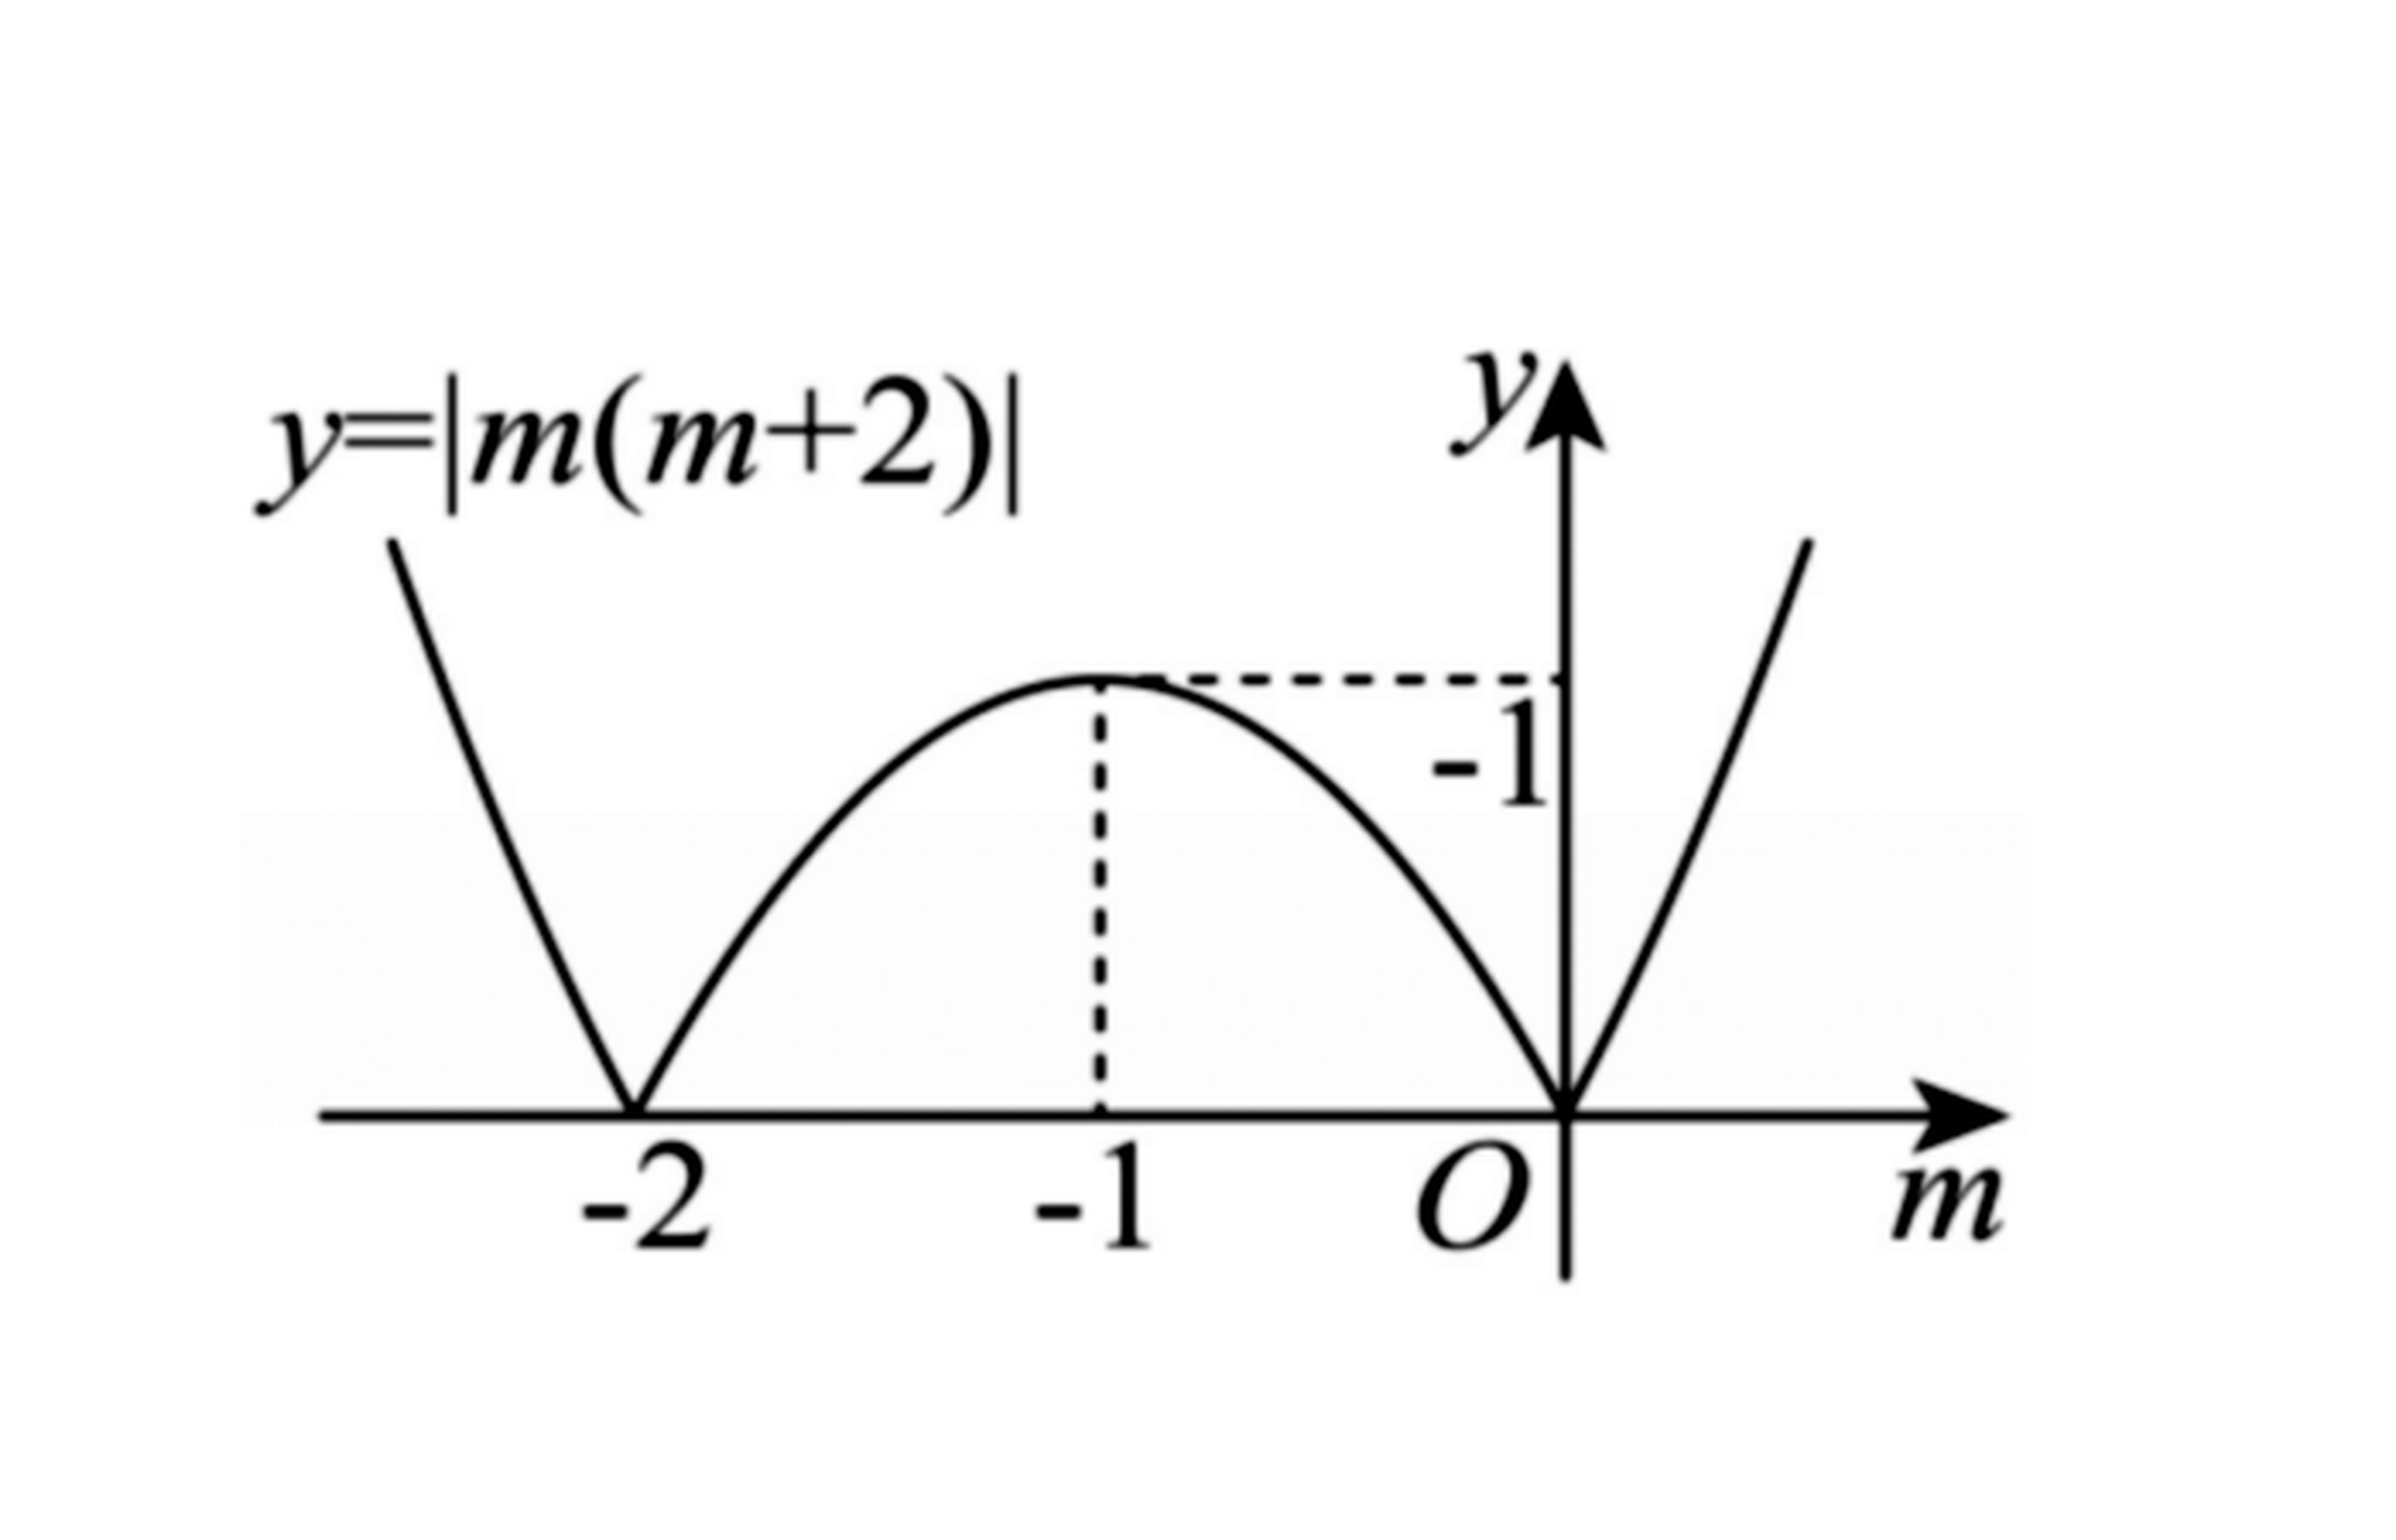
\includegraphics[width=0.46\textwidth]{figures/gao154_fujia2.png}
\end{center}
\step{由图像得 $k\in(0,1)$，}
\step{所以方程 $m^2+2m=k$ 和 $m^2+2m=-k$ 各有两个不同的根，}
\step{其中方程 $m^2+2m-k=0$ 的两根为 $m=-1\pm\sqrt{1+k}$，}
\step{方程 $m^2+2m+k=0$ 的两根为 $m=-1\pm\sqrt{1-k}$，}
\step{所以 $m_1=-1-\sqrt{1+k}$，$m_2=-1-\sqrt{1-k}$，$m_3=-1+\sqrt{1-k}$，$m_4=-1+\sqrt{1+k}$，且 $m_1<m_2<m_3<m_4$，}
\step{由 $m=\log_2 x$，则 $x=2^m$，}
\step{所以 $a=2^{-1-\sqrt{1+k}}$，$b=2^{-1-\sqrt{1-k}}$，$c=2^{-1+\sqrt{1-k}}$，$d=2^{-1+\sqrt{1+k}}$，}
\step{所以 $ad=2^{-1-\sqrt{1+k}}\times2^{-1+\sqrt{1+k}}=2^{(-1-\sqrt{1+k})+(-1+\sqrt{1+k})}=2^{-2}=\dfrac14$，}
\step{$b+c=2^{-1-\sqrt{1-k}}+2^{-1+\sqrt{1-k}}=\dfrac{2^{-\sqrt{1-k}}+2^{\sqrt{1-k}}}{2}$，}
\step{令 $s=\sqrt{1-k}$，其中 $s\in(0,1)$，则 $b+c=\dfrac12\left(2^{-s}+2^s\right)$，}
\step{设函数 $y=2^s+\dfrac1{2^s}$，令 $r=2^s\in(1,2)$，所以 $y=r+\dfrac1r$ 在 $(1,2)$ 上严格增，}
\step{所以函数 $y=2^s+\dfrac1{2^s}$ 在 $(0,1)$ 上严格增，所以 $y=2^s+\dfrac1{2^s}\in\left(2,\dfrac52\right)$，}
\step{所以 $b+c=\dfrac{2^{-s}+2^s}{2}\in\left(1,\dfrac54\right)$，$ad(b+c)=\dfrac{b+c}{4}\in\left(\dfrac14,\dfrac5{16}\right)$，}
\step{所以 $ad(b+c)$ 的取值范围是 $\left(\dfrac14,\dfrac5{16}\right)$，故选 $A$.}
\solend
\fi

\end{enumerate}

\end{document}
"
% 紧凑版：xelatex "\def\iscompact{1}% 高一154_徐汇中学_期中.tex
%   —— 高一上数学"2026-2027 年徐汇中学高一上期中"（试卷版/答案版/紧凑版）
% 试卷版：xelatex 高一154_徐汇中学_期中.tex
% 答案版：xelatex "\def\isanswer{1}% 高一154_徐汇中学_期中.tex
%   —— 高一上数学"2026-2027 年徐汇中学高一上期中"（试卷版/答案版/紧凑版）
% 试卷版：xelatex 高一154_徐汇中学_期中.tex
% 答案版：xelatex "\def\isanswer{1}% 高一154_徐汇中学_期中.tex
%   —— 高一上数学"2026-2027 年徐汇中学高一上期中"（试卷版/答案版/紧凑版）
% 试卷版：xelatex 高一154_徐汇中学_期中.tex
% 答案版：xelatex "\def\isanswer{1}\input{高一154_徐汇中学_期中.tex}"
% 紧凑版：xelatex "\def\iscompact{1}\input{高一154_徐汇中学_期中.tex}"
%
% ① 原始材料：微信公众号"魔都数学加油站"文章，连载"27学年高一154"，原文标题
% "27学年高一154——2026-2027年上海市徐汇中学高一上期中"；
% 原文链接：https://mp.weixin.qq.com/s/Qs2T7Zwsug-KKFE2wefDUg 。
% 正文为 12 张 PNG 页（01/03/04/05/07/11/12 为 2560×3620，
% 02/06/08/09/10 为 4762×6735，同一篇各页分辨率混排，逐页按各自分辨率裁图核对）。
% 体例：讲评版——一、填空题 3—12（10 题）、二、选择题 13—16（4 题）、
% 三、解答题 17—21（5 题）、附加题 1—2（2 题，原卷**另起编号**"1." "2."，
% 不与正题连号，同 高一a 成例），共 21 题；全卷每题均印【解析】
% （逐题核实，见 ② ②）。题目、答案、解析均据原图转录；卷面粉红色水印
% "魔都数学加油站"及公众号页脚未录入。
% 全卷插图清单（逐页通读 12 页确认）：3 组——
%   · Q15 题干配图（$f(x)=(x-a)(x-b)$ 抛物线，04 页右下：x/y 轴、O、1、
%     开口向上两零点均在 (0,1) 内），三版都出，裁 figures/gao154_q15_stem.png；
%   · Q15 四幅图像选项（05 页上半 2×2 排布，A/B/C/D 四幅指数函数图像，
%     合并成一张，照 高一136 Q13/Q22 成例），三版都出，
%     裁 figures/gao154_q15_opts.png；
%   · 附加题第 2 题解析配图（$y=\lvert m(m+2)\rvert$ 图像，11 页右上：
%     W 形折线、$-2$、$-1$、O、虚线 $y=1$ 与 $m=-1$），仅答案版出，
%     裁 figures/gao154_fujia2.png；
%   3 图均取自原卷截图，去粉色水印、去色、4× LANCZOS 放大；Q15 题干图
%   左侧题干残字"的图"已裁白。其余各页逐页确认无其它题目配图、无表格；
%   12 页下半仅水印、无正文。
%
% 卷首标题：原卷印作"2026-2027 年徐汇中学高一上期中"，年份区间按全稿惯例排 en dash；
% 原卷卷面未印副标题，本稿按同期中卷知识模块口径补出"集合与常用逻辑用语、不等式、函数"。
%
% ② 与原卷的排版差异：
%   ① 原文从第 3 题起，本稿保留原题号；共 21 题四节，正题到 21，附加题另起编号
%      1—2（\bigsec{附加题} 后 \begin{enumerate} 不 \setcounter，同 高一a 成例）；
%   ② 全 21 题均印【解析】、用 \solbegin…\solend，无只印【答案】或答案印括号内的题；
%      四道正题选择题答案在解析末句"故选 C／A／B／C"（Q13—Q16）、附加题第 2 题
%      答案在解析末句"故选 A"，括号 \mbox{（\quad）} 留空、不另提 \ans{}；
%      答案版【答案】/【解析】标记数 = 21 = 全卷题数；
%   ③ 原卷卷面未印副标题，本稿按知识模块口径补出；
%   ④ 原卷填空横线按全稿惯例排 \blankline[4.4em]；选择题括号排 \mbox{（\quad）}、
%      四道正题选择题与附加题第 2 题的选项段前按惯例各加 \keepwithprev
%      （Q15 与附加题 2 的选项段是整块图，\keepwithprev 后接 \begin{center}）；
%      解答题不留作答区、不加 \anspace（原卷为讲评版）；
%   ⑤ 数集黑板粗体：Q4"$x,y\in R$"、Q9"$x\in\R$"、Q13 无、
%      Q15"定义域 $\R$"、Q19"$\forall x\in\R$"、Q21"$x\in\N$"与"$k\in\N^*$"、
%      Q20"$a,b\in\R$"、附加题 2 无——原卷印斜体或正体粗体 R/N/N*，
%      按全稿惯例归一 \R／\N／\N^*；绝对值排 \lvert…\rvert
%      （Q5、Q9、Q12、Q13、Q16、Q21、附加题 2），集合描述竖线排 \mid
%      （Q5、Q17、Q19、Q21），不等号按全稿惯例排 \leqslant／\geqslant；
%      空集 \varnothing（Q21 题干 (3)）；
%   ⑥ 子集符号逐处照录、不得统一：Q6 题干印"$\{1,2\}\subset M\subseteq\{1,2,3,4,5\}$"
%      （前单线 ⊂、后带下划线 ⊆，同句两形并用），解析亦两形并用；
%      Q17 解析 (2)"$B\subset A$"印单线 ⊂；Q21 题干 (3)"$A\subseteq\{x\mid\cdots\}$"
%      印带下划线 ⊆——逐处放大核，分别 \subset／\subseteq，照录未统一（见 ④）；
%   ⑦ 判别式 Δ/△：Q18 解析 (1)"$\Delta=m^2-4(4m^2-3)$"与 Q19 解析 (1)
%      "$\Delta=4m^2-8m<0$"两处均印等腰偏高粗三角、照录 \Delta；本卷无扁等边
%      细线 \triangle 用例（见 ④）；
%   ⑧ 中文弯引号照录：Q4"设 $x$、$y\in\R$. 若 $x+y>2$，则 $x>1$ 或 $y>1$"、
%      附加题 1"$n$ 元集和集"与"3 元集和集"；注释里一律 ASCII 引号；
%      数学式内 CJK 用 \text{}（Q5 解集描述"或"、Q19 集合描述的"或"）；
%   ⑨ "图像／图象"逐处放大核：Q15 题干与解析印"图象"（象，无亻）、
%      Q16 无、附加题 2 解析印"图象"与"图像"（"画出函数…的图象"、
%      "由图像得"——两形并用，逐处照录未统一）；Q13/Q14 无数集图像字样；
%      半角逗号在数学组之间是全稿惯例、非笔误，逐处照录（Q3、Q10、Q16、
%      Q18、Q20、Q21 的 $x_1,x_2$ 之类）；行末西文句点 ASCII `.`；
%      行中全角逗号／顿号照录（Q6"3，4，5"、Q20"（单位：元）"、
%      附加题 1"$a_1,a_2,a_3,a_4$"）；
%   ⑩ 复杂式照录别简化：Q3 $a^{\frac{12}{7}}\cdot\left(\frac17\right)^{\frac17}
%      \cdot\sqrt[7]{a^4}$ 与 $7^{-\frac17}a^{\frac{16}{7}}$、Q7 $x^{-m}$、
%      Q8 $\frac{b-2a+2}{2a}$、Q11 $\frac{9+4\sqrt2}{6}$、Q12 $506\frac29$ 与
%      $506\frac49$、Q16 高斯取整 $[a]$、Q20 $c(x)=10x+\frac1{100}x^2$ 与
%      $q(x)=a+\frac xb$、Q21 $A^+$／$A^-$ 与 $|A^+|\geqslant2k-1$、
%      附加题 2 $m=-1\pm\sqrt{1+k}$ 与 $ad(b+c)$；
%      \left…\right 不得拆到不同 $…$ 组（Q5 $\left\{x\mid\cdots\right\}$、
%      Q20 $\left(\frac1b-\frac1{100}\right)$、附加题 2 $\left(\frac14,\frac5{16}\right)$）；
%      cases 块一律 \begin{cases}…\end{cases}；
%   ⑪ 一条 \step = 原卷解析的一个印刷行，cases 块整体算一个印刷行；别并折行、
%      别拆行。Q11 九行、Q12 六行、Q16 十六行、Q20 十一行、Q21 十七行、
%      附加题 2 十八行均按印刷行逐条断，不丢行；
%   ⑫ 配图：Q15 题干小图（三版都出）放 \item 内题干之后 \begin{center}，
%      Q15 四幅选项图（三版都出）放 \keepwithprev 之后的 \begin{center}，
%      Q15 用 \needvspace 守卫把"题干＋两图"整块推走（守卫放 \item 之前，
%      见 高一145 Q14/Q20 与 高一136 Q13 成例）；附加题 2 解析配图（仅答案版出）
%      放 \ifanswer 内 \solbegin…\solend 的 \step 之间（高一73 第 16 题成例）；
%   ⑬ 原卷解析内无红色"法一／法二"之类小标题，故本卷无 \stepm；红色水印
%      "魔都数学加油站"不录入；
%   ⑭ 跨页续印按题合并：见 ⑥；
%
% ③ 行数复核：一条 \step = 原卷解析的一个印刷行，cases 块作一个印刷行计。
%   逐题数（主会话逐页核对定稿）：Q3：1；Q4：1；Q5：3；Q6：4；Q7：3；
%   Q8：1；Q9：5；Q10：4；Q11：9；Q12：6；Q13：5；Q14：4；Q15：3；
%   Q16：16；Q17：5；Q18：9；Q19：10；Q20：11；Q21：17；
%   附加题 1：6；附加题 2：18。
%   合计 141 条 \step（本卷无 \stepm），与原卷逐题印刷行相等。全卷 21 题
%   均设 \solbegin…\solend，答案版【答案】/【解析】标记数 = 21 = 全卷题数。
%
% ④ 判别式／子集符号结论（逐处放大原图照录、不得统一，主会话像素级复核）：
%   判别式：Q18 解析 (1)"$\Delta=m^2-4(4m^2-3)=-15m^2+12\geqslant0$"、
%      Q19 解析 (1)"$\Delta=4m^2-8m<0$"共 2 处，逐处放大确认印等腰偏高
%      粗三角（高>宽、右斜边粗），照录 \Delta；本卷无扁等边细线 \triangle
%      用例，无几何三角形符号。
%   子集：Q6 题干"$\{1,2\}\subset M\subseteq\{1,2,3,4,5\}$"前 ⊂ 单线、
%      后 ⊆ 带下划线（/tmp/gao154/z/zoom/q6_subset.png），解析两处同样两形
%      并用，分别照录 \subset／\subseteq；Q17 解析 (2)"$B\subset A$"单线
%      照录 \subset；Q21 题干 (3)"$A\subseteq\{x\mid\cdots\}$"带下划线
%      照录 \subseteq。本卷 ⊂ 与 ⊆ 混用逐处照录、不得统一。
%      空集 \varnothing（Q21 题干 (3)）、数集 \R／\N／\N^* 归一见 ② ⑤。
%
% ⑤ 存疑照录（放大原图确认，照录未改、正文对应处另有 % 注）：
%   1. Q7 题干印 $f(x)=(3m-1)x^{-m}$，解析首句却写"幂函数 $f(x)=x^\alpha$
%      的系数必须为 1"（用 $\alpha$ 作指数记号），随后 $f(2)=2^\alpha=8$
%      得 $\alpha=3$、$f(x)=x^3$——题干指数 $-m$ 与解析 $\alpha$ 记法不同，
%      系原卷记号前后不一，逐处照录未统一（放大 01/02 页确认）。
%   2. Q11 解析"因为 $u>0,v>0$，由基本不等式得 $\frac{4v}{u}+\frac{2u}{v}
%      \geqslant2\sqrt{\frac{4v}{u}\cdot\frac{2u}{v}}=4\sqrt2$"与
%      "所以 $\frac4u+\frac1v=\frac16\left(\frac4u+\frac1v\right)(2u+v)$"
%      照录，未把 $u,v$ 化简回 $x,y$。
%   3. Q16 解析把"$[a]$ 表示不超过 $a$ 的最大整数"与"和至少有一个不小于 2"
%      连写在同一行（原卷如此），照录未改；末行"假设成立，C 正确，D 错误"照录。
%   4. Q18 解析 (2)"函数 $y=-7m^2+6$ 开口向下，对称轴为 $m=0$"却称求
%      "$y_{\min}$"（实为在 $m^2\leqslant\frac45$ 闭区间上的最小值），
%      照录未改。
%   5. Q20 题干"$q(x)=a+\frac xb$（$a,b\in\R$）"与解析
%      "$W(x)=\left(\frac1b-\frac1{100}\right)x^2+(a-10)x-160000$"照录；
%      末行解得 $a=90,b=\frac{500}{3}$ 照录未化简。
%   6. Q21 题干 (3)"$A\subseteq\{x\mid0\leqslant x\leqslant2020,x\in\N\}$"
%      与解析"$3k-1\leqslant2a_k+1\leqslant4041$（$k\in\N^*$）"照录；
%      末行"集合 $A$ 中元素的个数的最大值是 1347"照录。
%   7. 附加题 1 解析"相加化简得 $a_1+a_2+a_3+a_4=5$"照录；
%      附加题 2 解析"由图像得 $k\in(0,1)$"与"由图像得"／"的图象"两形
%      并用逐处照录（见 ② ⑨）；末行"$ad(b+c)$ 的取值范围是
%      $\left(\frac14,\frac5{16}\right)$，故选 A"照录。
%   全卷除此 7 类外未发现其它笔误／自相矛盾处；21 题均印【解析】、
%   无只印【答案】或答案印括号内的题（见 ② ②）。
%
% ⑥ 跨页续印按题合并说明（逐页核实定稿）：Q3—Q5 题干＋解析在 01 页
%   （Q5 解析末 2 行续 01 页下半）；Q6、Q7 题干＋解析在 01 页下半
%   （Q7 解析余 2 行续 02 页顶）；Q8、Q9 题干＋解析在 02 页上半
%   （Q9 解析余 3 行续 02 页下半）；Q10 题干＋解析在 02 页下半；
%   Q11 题干＋解析前 6 行在 03 页上半、余 3 行续 03 页下半；
%   Q12 题干＋解析前 5 行在 03 页下半、末行续 04 页顶；"二、选择题"
%   标题与 Q13 题干＋选项＋解析在 04 页上半；Q14 题干＋选项＋解析、
%   Q15 题干＋题干配图在 04 页下半；Q15 四幅选项图＋解析、
%   Q16 题干＋选项＋解析首行在 05 页上半，Q16 解析余 12 行在
%   05 页下半—06 页上半；"三、解答题"标题与 Q17 题干＋两问＋解析
%   在 06 页下半；Q18 题干＋两问＋解析在 07 页上半—下半；
%   Q19 题干＋两问＋解析首行在 07 页下半，解析余 8 行在 08 页上半；
%   Q20 题干在 08 页下半，解析 (1) 4 行＋(2) 首 4 行在 08 页下半—09 页上半，
%   (2) 余 2 行在 09 页下半；Q21 题干＋三问＋解析 (1)(2) 4 行在
%   09 页下半—10 页上半，解析 (3) 余 12 行在 10 页上半—下半；
%   "附加题"标题与附加题 1 题干＋解析首 3 行在 10 页下半，
%   余 3 行续 11 页上半；附加题 2 题干＋选项＋解析前 3 行在 11 页上半，
%   解析配图＋余 12 行在 11 页下半—12 页上半，末行
%   "所以 $ad(b+c)$ 的取值范围是 $\left(\frac14,\frac5{16}\right)$，故选 A"
%   为全卷收尾（12 页下半仅水印、无正文）。
%   本稿按题连排，不丢行、不并折行；全卷末题为附加题第 2 题。
%
\documentclass[a4paper,11pt]{article}
\usepackage{common}

\begin{document}

\examtitlest[3]{2026--2027 年徐汇中学高一上期中}{集合与常用逻辑用语、不等式、函数}

\bigsec{一、填空题}

\begin{enumerate}
\setcounter{enumi}{2}

% === Q3 === 分数指数幂照录；解析 1 行
\item 已知 $a>0$，化简 $a^{\frac{12}{7}}\cdot\left(\dfrac17\right)^{\frac17}\cdot\sqrt[7]{a^4}=$\blankline[4.4em].

\ifanswer
\solbegin
\step{$a^{\frac{12}{7}}\cdot\left(\dfrac17\right)^{\frac17}\cdot\sqrt[7]{a^4}=a^{\frac{12}{7}}\cdot(7^{-1})^{\frac17}\cdot a^{\frac47}=7^{-\frac17}a^{\frac{16}{7}}$.}
\solend
\fi

% === Q4 === 反证法；中文弯引号照录；解析 1 行
\item 用反证法证明命题：“设 $x$、$y\in\R$. 若 $x+y>2$，则 $x>1$ 或 $y>1$”时，假设的内容应该是\blankline[4.4em].

\ifanswer
\solbegin
\step{由反证法得，假设的内容应该是 $x\leqslant1$ 且 $y\leqslant1$.}
\solend
\fi

% === Q5 === 分式不等式；cases 块；解析 3 行
\item 不等式 $\dfrac{2x+3}{x-1}\geqslant1$ 的解集为\blankline[4.4em].

\ifanswer
\solbegin
\step{$\dfrac{2x+3}{x-1}\geqslant1$，即 $\dfrac{2x+3}{x-1}-1\geqslant0$，$\dfrac{x+4}{x-1}\geqslant0$，}
\step{等价于 $\begin{cases}(x+4)(x-1)\geqslant0\\x-1\ne0\end{cases}$，解得 $x>1$ 或 $x\leqslant-4$，}
\step{故解集为 $\{x\mid x>1\text{ 或 }x\leqslant-4\}$.}
\solend
\fi

% === Q6 === ⊂ 与 ⊆ 并用照录；解析 4 行
\item 满足条件 $\{1,2\}\subset M\subseteq\{1,2,3,4,5\}$ 的集合 $M$ 的个数为\blankline[4.4em].

\ifanswer
\solbegin
\step{因为 $\{1,2\}\subset M\subseteq\{1,2,3,4,5\}$，所以集合 $M$ 必含有元素 1，2，}
\step{且至少含有元素 3，4，5 中的一个，}
\step{则集合 $M$ 的个数与集合 $\{3,4,5\}$ 的非空子集的个数一样，}
\step{所以集合 $M$ 的个数为 $2^3-1=7$.}
\solend
\fi

% === Q7 === 题干 $x^{-m}$、解析用 $x^\alpha$ 记法，原卷记号差异照录（见 ⑤ 1）；解析 3 行
\item 已知幂函数 $f(x)=(3m-1)x^{-m}$，且 $f(2)=8$，则 $f(m)=$\blankline[4.4em].

\ifanswer
\solbegin
\step{幂函数 $f(x)=x^\alpha$ 的系数必须为 1，所以 $3m-1=1$，得 $m=\dfrac23$.}
\step{又 $f(2)=2^\alpha=8=2^3$，故 $\alpha=3$，即 $f(x)=x^3$，}
\step{所以 $f(m)=f\left(\dfrac23\right)=\left(\dfrac23\right)^3=\dfrac8{27}$.}
\solend
\fi

% === Q8 === 换底公式；解析 1 行
\item 已知 $a=\lg2$，$b=\lg3$，用含 $a,b$ 的代数式表示 $\log_4 75=$\blankline[4.4em].

\ifanswer
\solbegin
\step{$\log_4 75=\dfrac{\lg\left(3\times\frac{10^2}{2^2}\right)}{\lg2^2}=\dfrac{\lg3+2-2\lg2}{2\lg2}=\dfrac{b-2a+2}{2a}$.}
\solend
\fi

% === Q9 === 三角不等式取等；解析 5 行
\item 设 $x\in\R$，则方程 $\lvert x-2\rvert+\lvert3x+1\rvert=\lvert2x+3\rvert$ 的解集是\blankline[4.4em].

\ifanswer
\solbegin
\step{由 $\lvert x-2\rvert=\lvert2-x\rvert$，故原方程可化为 $\lvert2-x\rvert+\lvert3x+1\rvert=\lvert2x+3\rvert$，}
\step{又 $(2-x)+(3x+1)=2x+3$，}
\step{由三角不等式 $\lvert2-x\rvert+\lvert3x+1\rvert\geqslant\lvert(2-x)+(3x+1)\rvert=\lvert2x+3\rvert$，}
\step{当且仅当 $(2-x)(3x+1)\geqslant0$ 等号成立，}
\step{解 $(2-x)(3x+1)\geqslant0$ 得 $-\dfrac13\leqslant x\leqslant2$，故原方程的解集为 $\left[-\dfrac13,2\right]$.}
\solend
\fi

% === Q10 === 韦达定理；cases 块；解析 4 行
\item 已知一元二次不等式 $x^2+bx+c>0$ 的解集为 $(-\infty,-1)\cup(2,+\infty)$，则一元二次不等式 $bx^2+cx-1<0$ 的解集是\blankline[4.4em].

\ifanswer
\solbegin
\step{因为 $x^2+bx+c>0$ 的解集为 $(-\infty,-1)\cup(2,+\infty)$，}
\step{所以方程 $x^2+bx+c=0$ 的两根为 $-1$ 和 2，则有 $\begin{cases}-b=-1+2\\c=-1\times2\end{cases}$，即 $\begin{cases}b=-1\\c=-2\end{cases}$，}
\step{则 $bx^2+cx-1<0$ 等价于 $-x^2-2x-1<0$，得 $x^2+2x+1>0$，得 $(x+1)^2>0$，}
\step{解得 $x\ne-1$，故不等式 $bx^2+cx-1<0$ 的解集为 $(-\infty,-1)\cup(-1,+\infty)$.}
\solend
\fi

% === Q11 === 换元 $u,v$；解析 9 行
\item 已知正数 $x,y$ 满足 $2x+y=1$，则 $\dfrac4{x+2}+\dfrac1{y+1}$ 的最小值为\blankline[4.4em].

\ifanswer
\solbegin
\step{令 $u=x+2$，$v=y+1$，则 $u>2$，$v>1$，}
\step{且 $2u+v=2(x+2)+(y+1)=2x+y+5=6$.}
\step{因为 $u>0$，$v>0$，由基本不等式得 $\dfrac{4v}{u}+\dfrac{2u}{v}\geqslant2\sqrt{\dfrac{4v}{u}\cdot\dfrac{2u}{v}}=4\sqrt2$，}
\step{所以 $\dfrac4u+\dfrac1v=\dfrac16\left(\dfrac4u+\dfrac1v\right)(2u+v)=\dfrac16\left(9+\dfrac{4v}{u}+\dfrac{2u}{v}\right)\geqslant\dfrac{9+4\sqrt2}{6}$，}
\step{当且仅当 $\dfrac{4v}{u}=\dfrac{2u}{v}$，即 $u=\sqrt2v$ 时等号成立，}
\step{与 $2u+v=6$ 联立得 $u=\dfrac{6\sqrt2}{2\sqrt2+1}$，$v=\dfrac6{2\sqrt2+1}$，}
\step{此时 $x=u-2=\dfrac{2\sqrt2-2}{2\sqrt2+1}>0$，$y=v-1=\dfrac{5-2\sqrt2}{2\sqrt2+1}>0$，且 $2x+y=1$，}
\step{满足题设，所以下界可以取得，}
\step{因此 $\dfrac4{x+2}+\dfrac1{y+1}$ 的最小值为 $\dfrac{9+4\sqrt2}{6}$.}
\solend
\fi

% === Q12 === 2025 个整数解；解析 6 行
\item 若关于 $x$ 的不等式 $\lvert x-2k\rvert+\lvert x-3k\rvert<4k$ 共有 2025 个整数解，则实数 $k$ 的取值范围为\blankline[4.4em].

\ifanswer
\solbegin
\step{显然 $k>0$，由 $\lvert x-2k\rvert+\lvert x-3k\rvert<4k$，得 $\dfrac12k<x<\dfrac92k$，}
\step{因为该不等式共有 2025 个整数解，所以 $2024<\dfrac{9k}{2}-\dfrac k2\leqslant2026$，}
\step{解得 $506<k\leqslant506.5$，}
\step{由 $\dfrac k2\in(253,253.25]$，得这 2025 个整数解只能为 254、255、256、$\cdots$、2278，}
\step{所以 $2278<\dfrac{9k}{2}\leqslant2279$，解得 $506\dfrac29<k\leqslant506\dfrac49$，结合 $506<k\leqslant506.5$，}
\step{得 $k$ 的取值范围是 $\left(506\dfrac29,506\dfrac49\right]$.}
\solend
\fi

\end{enumerate}

\bigsec{二、选择题}

\begin{enumerate}
\setcounter{enumi}{12}

% === Q13 === 四选项一行；解析 5 行，故选 C
\item 若 $a<b<0$，则下列不等式中不成立的是\mbox{（\quad）}

\keepwithprev
A. $a-b>a$\qquad B. $\dfrac1a>\dfrac1b$\qquad C. $a^3>b^3$\qquad D. $\lvert a\rvert>\lvert b\rvert$

\ifanswer
\solbegin
\step{A 选项，因为 $b<0$，所以 $-b>0$，不等式两边同加上 $a$ 得 $a-b>a$，故 A 正确；}
\step{B 选项，因为 $a<b<0$，所以 $ab>0$，不等式两边同除以 $ab$，则 $\dfrac1b<\dfrac1a<0$，故 B 正确；}
\step{C 选项，不妨设 $a=-2$，$b=-1$，则 $a^3=-8$，$b^3=-1$，故 $a^3<b^3$，故 C 错误；}
\step{D 选项，因为 $a<b<0$，所以 $-a>-b$，即 $\lvert a\rvert>\lvert b\rvert$，故 D 正确.}
\step{故选 $C$.}
\solend
\fi

% === Q14 === 选项两行两列；解析 4 行，故选 A
\item 设命题 $p:x^2-5x+4\ne0$，命题 $q:x\ne1$，则 $p$ 是 $q$ 的\mbox{（\quad）}条件

\keepwithprev
A. 充分不必要\qquad\qquad B. 必要不充分

C. 充要\qquad\qquad D. 既不充分也不必要

\ifanswer
\solbegin
\step{$p:x^2-5x+4\ne0\Leftrightarrow(x-1)(x-4)\ne0\Leftrightarrow x\ne1$ 且 $x\ne4$；$q:x\ne1$.}
\step{充分性：当 $x\ne1$ 且 $x\ne4$ 时，$x\ne1$，所以 $p\Rightarrow q$；}
\step{必要性：当 $x\ne1$ 时，若 $x=4$，此时 $p$ 不成立，即 $q\nRightarrow p$；}
\step{所以 $p$ 是 $q$ 的充分不必要条件，故选 $A$.}
\solend
\fi

% === Q15 === 题干配图（三版都出）+ 四幅图像选项（2×2 合并，三版都出）；守卫放 \item 之前；解析 3 行，故选 B
\needvspace{9cm}
\item 已知函数 $f(x)=(x-a)(x-b)$（$a<b$）的图象如图所示，则函数 $g(x)=a^x-b$ 的图象可能是\mbox{（\quad）}

\begin{center}
% 抛物线题干配图取 04 页右下，去粉色水印、去色、4× LANCZOS 放大；三版都出
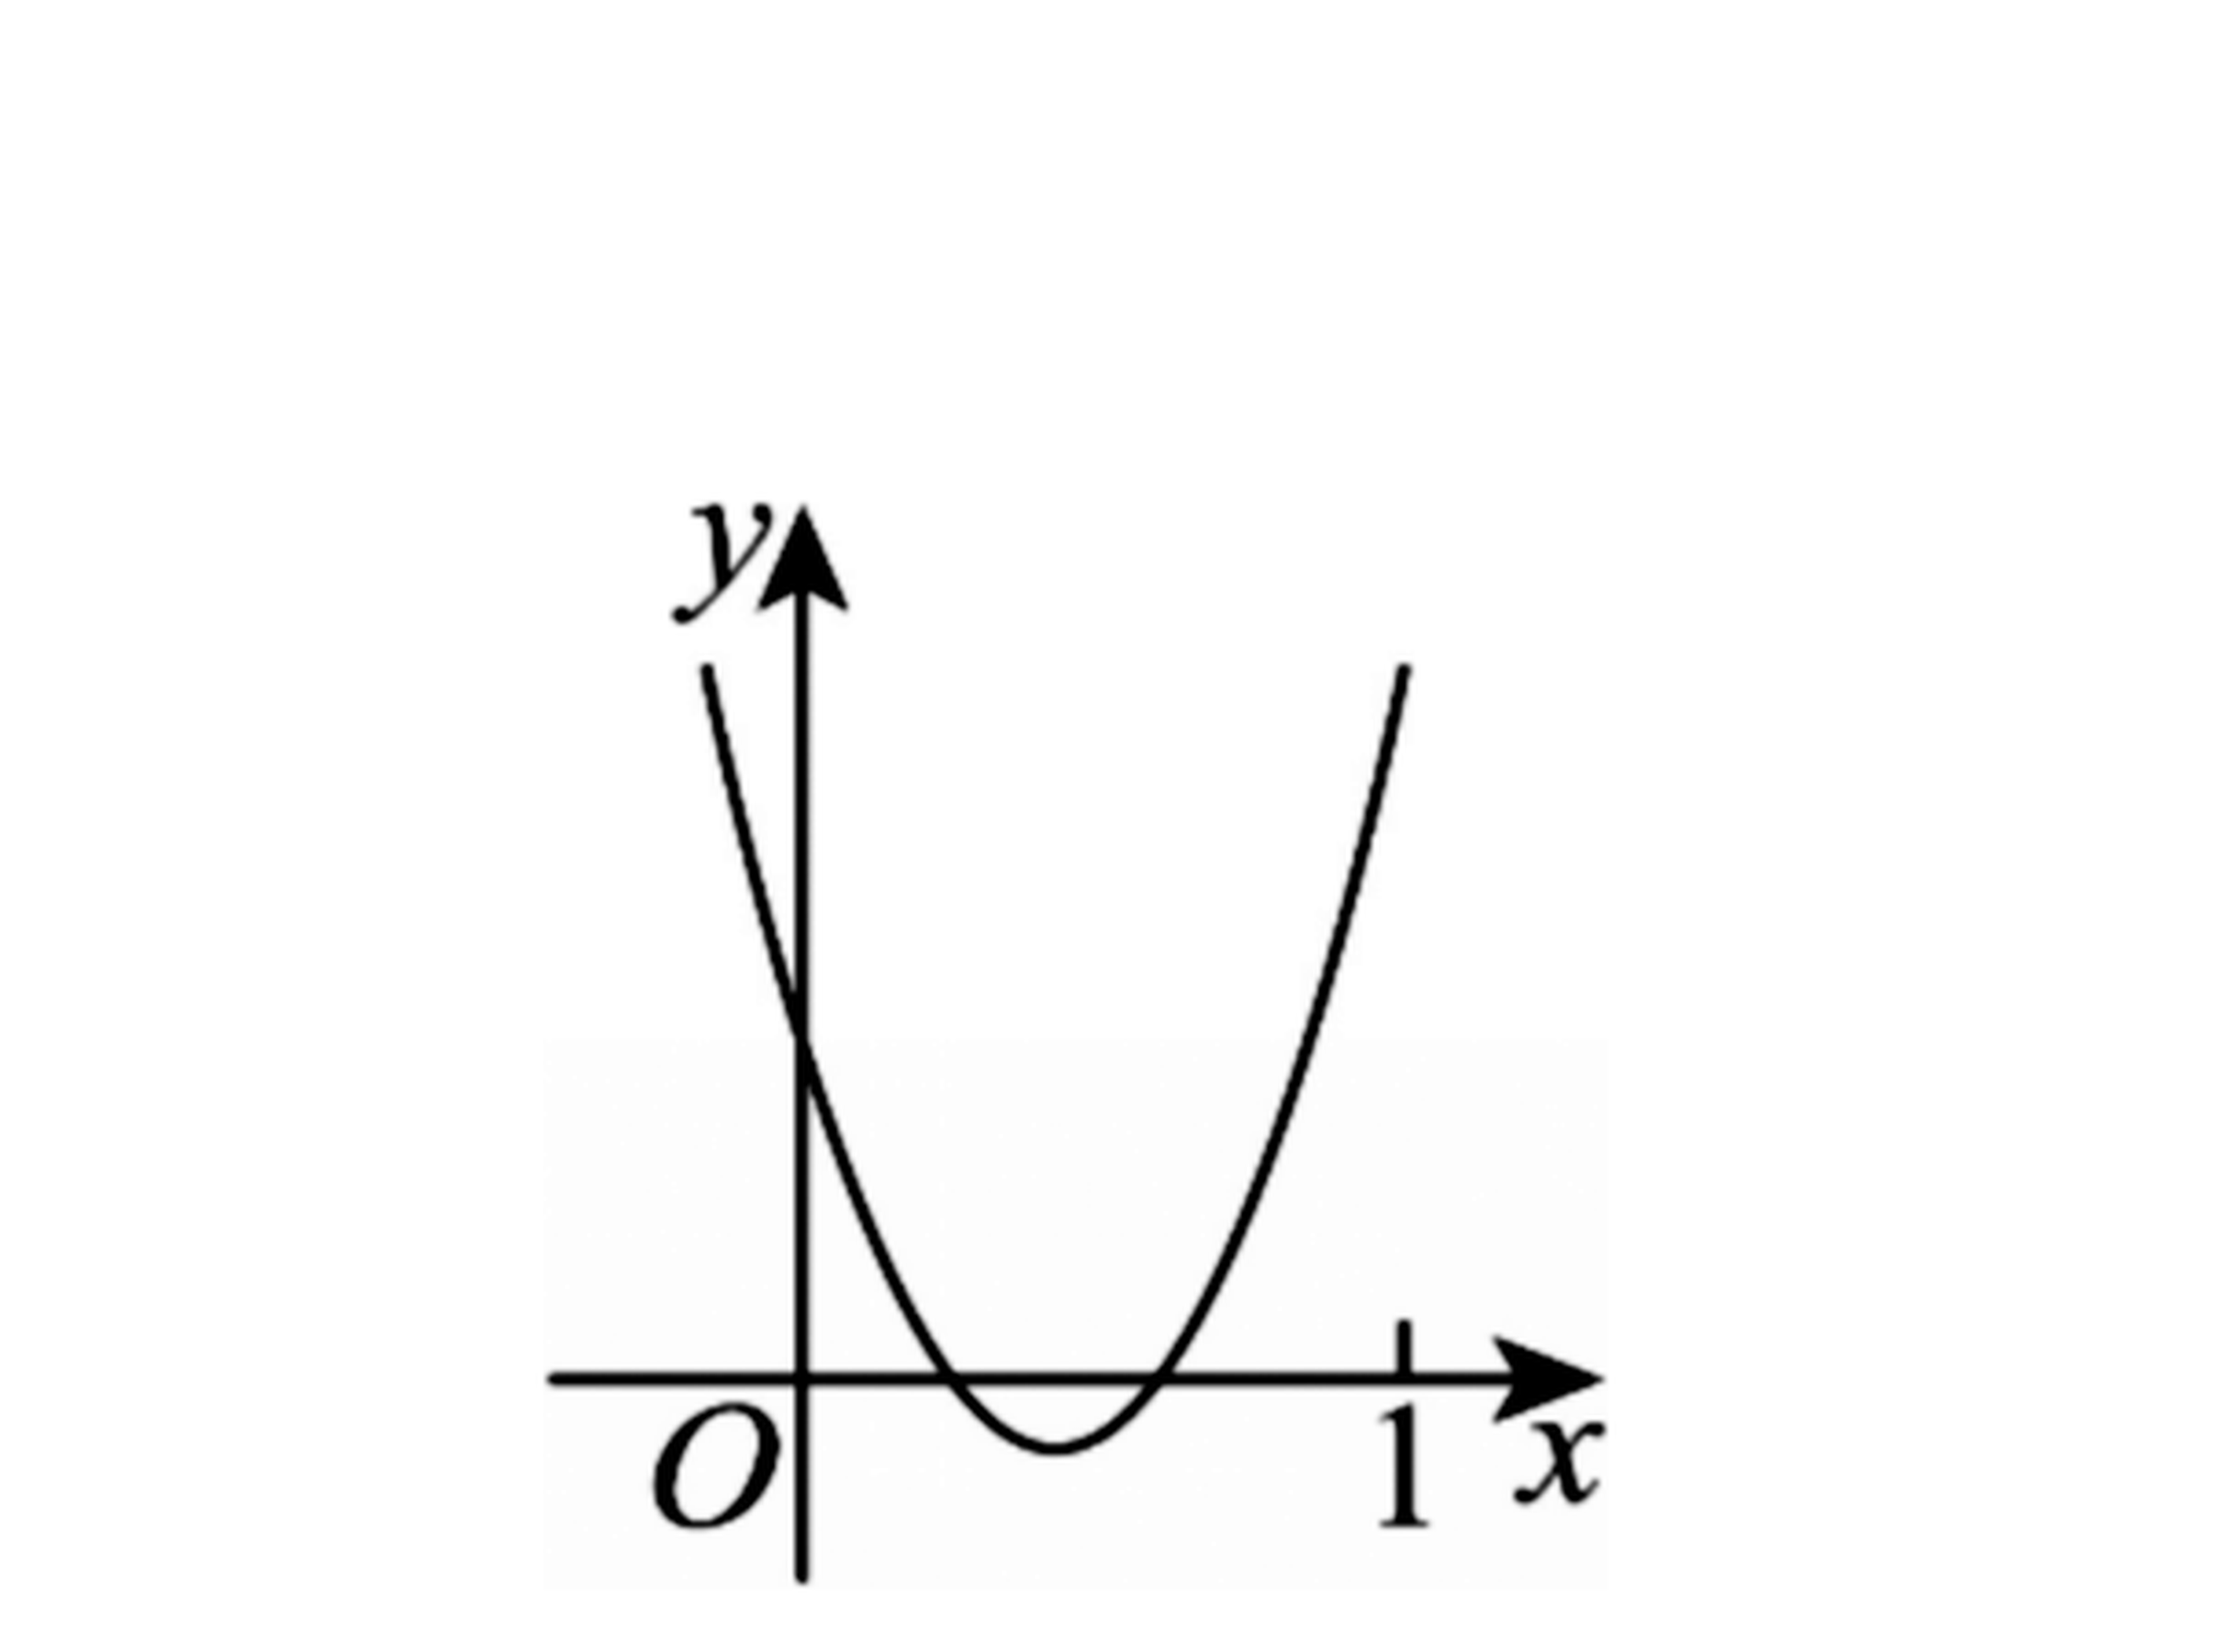
\includegraphics[width=0.32\textwidth]{figures/gao154_q15_stem.png}
\end{center}

\keepwithprev
\begin{center}
% 四幅指数函数图像选项取 05 页上半，按原卷 2×2 排布合并为一张，去粉色水印、去色、4× LANCZOS 放大；三版都出
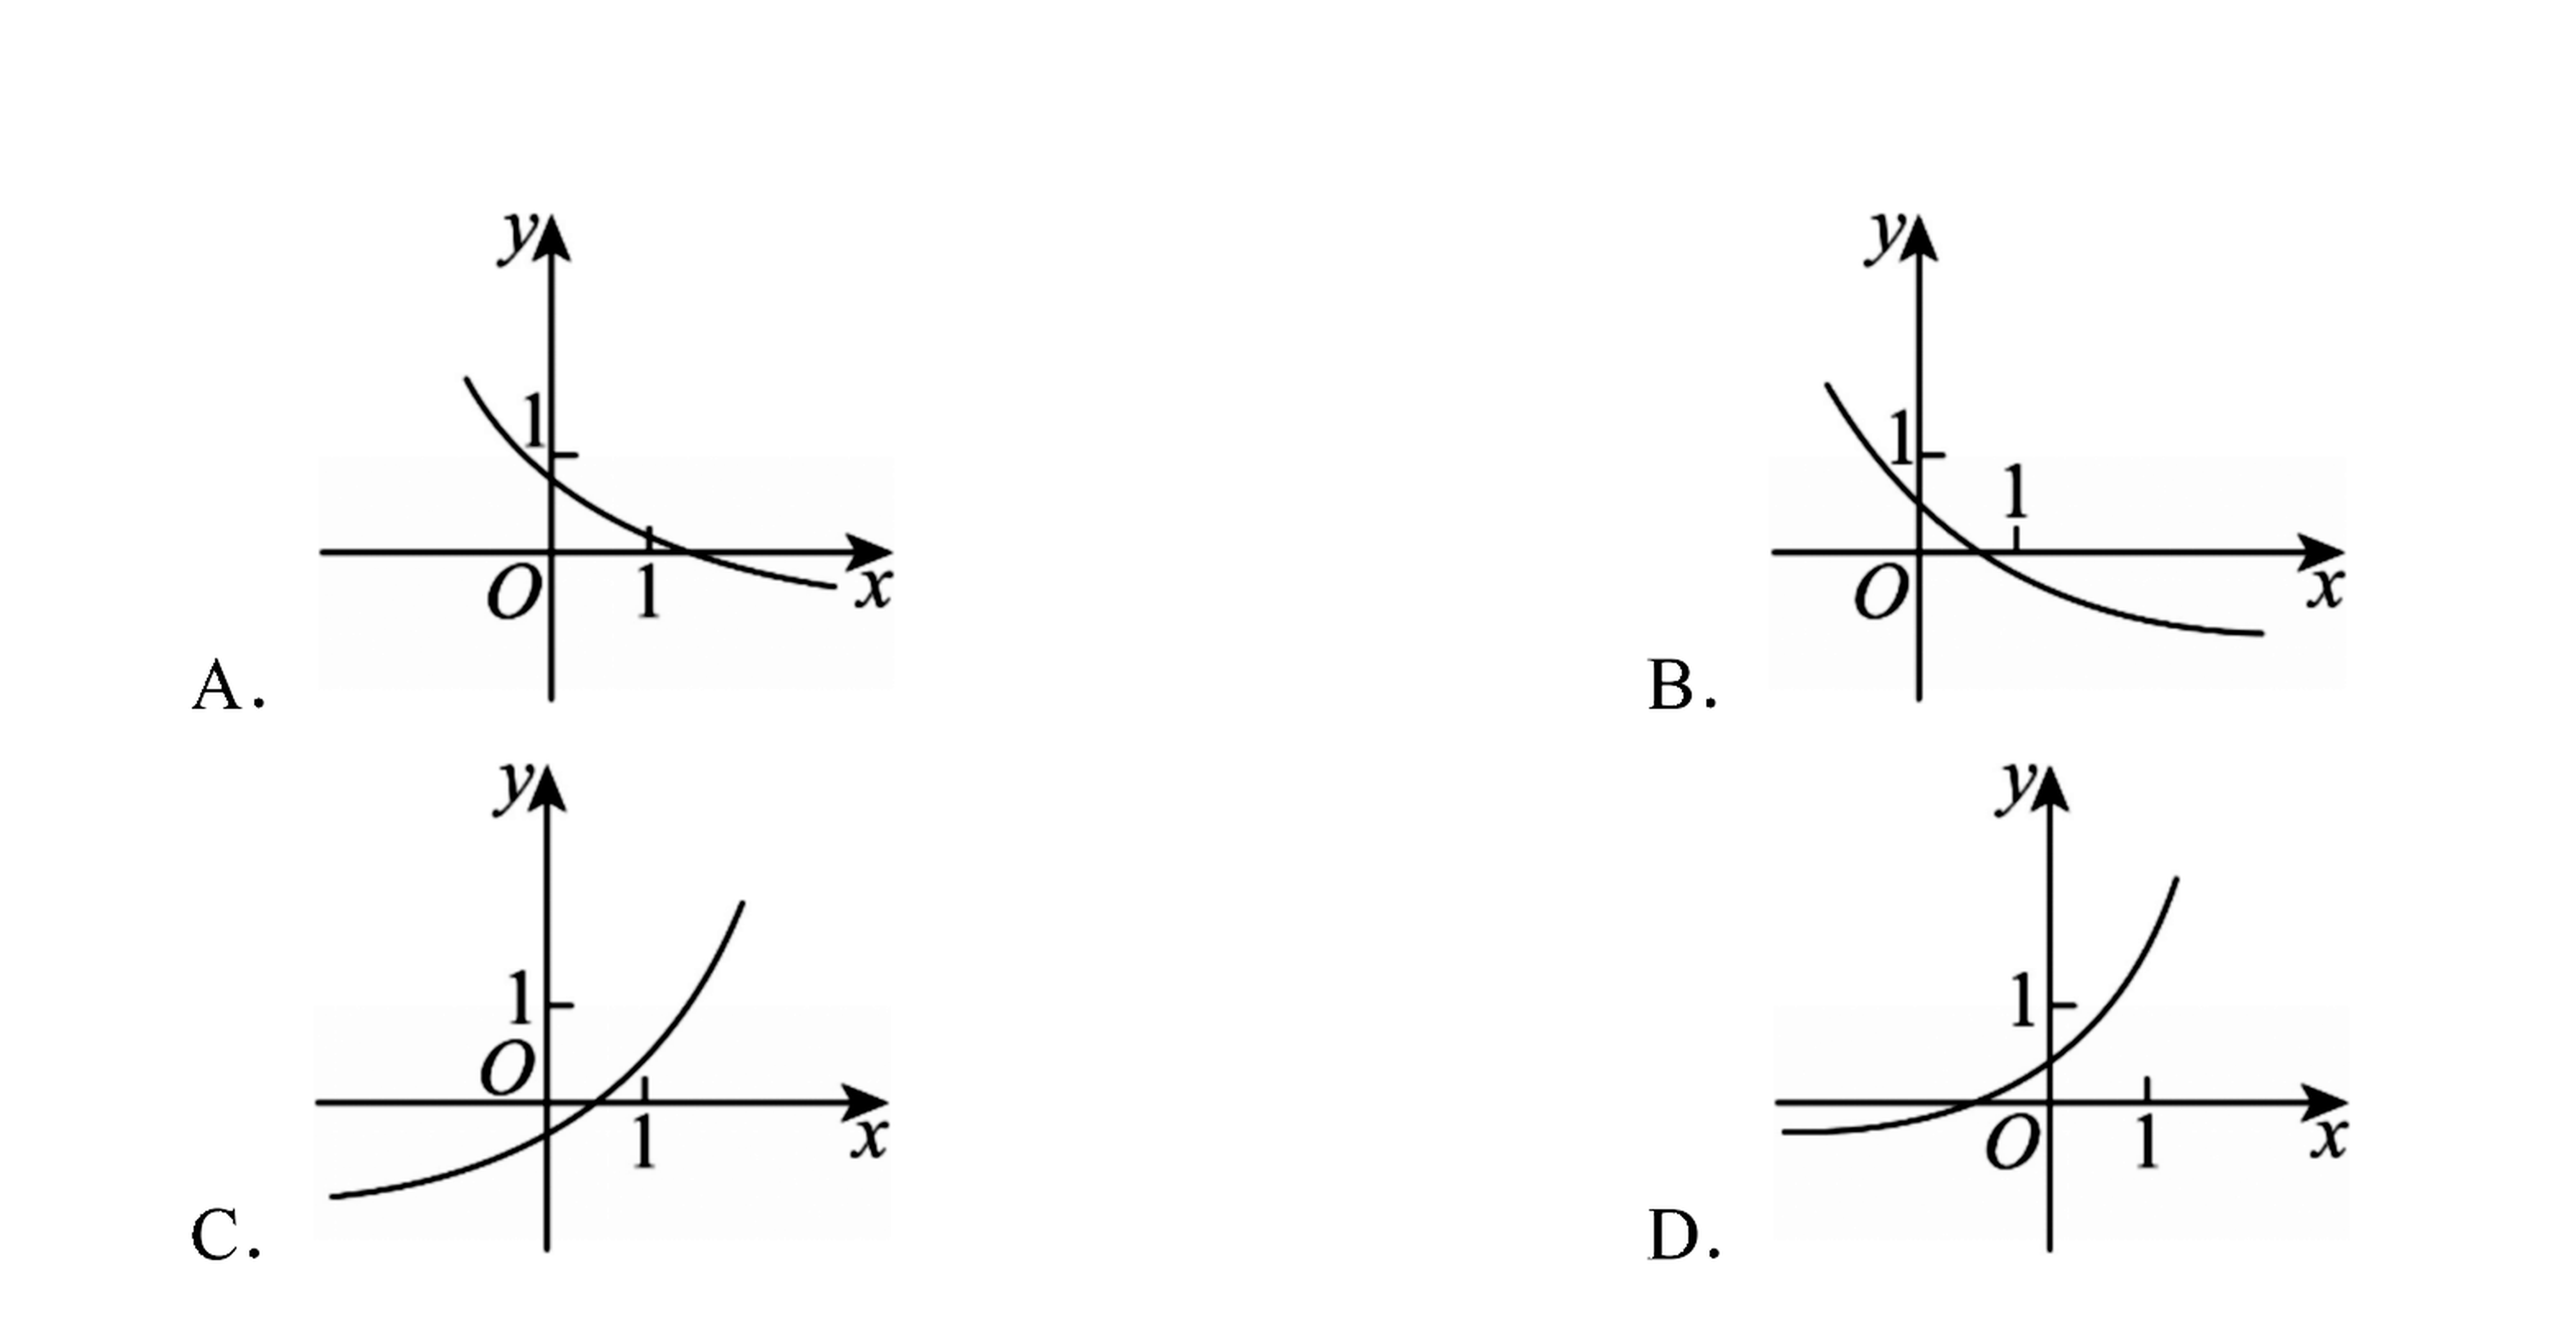
\includegraphics[width=0.80\textwidth]{figures/gao154_q15_opts.png}
\end{center}

\ifanswer
\solbegin
\step{由题意得 $0<a<b<1$，所以 $g(x)=a^x-b$ 在定义域 $\R$ 上严格减.}
\step{$g(0)=a^0-b=1-b>0$，$g(1)=a^1-b=a-b<0$，故 B 符合题意.}
\step{故选 $B$.}
\solend
\fi

% === Q16 === 高斯取整；解析 13 行，故选 C
\item 设 $[a]$ 表示不超过 $a$ 的最大整数，如 $[1.2]=1$，$[-3.2]=-4$，若 $x$、$y$、$z$ 为正实数，则 $\left[\dfrac{y+z}{x}\right]+\left[\dfrac{z+x}{y}\right]+\left[\dfrac{x+y}{z}\right]$ 的最小值为\mbox{（\quad）}

\keepwithprev
A. 2\qquad\qquad B. 3\qquad\qquad C. 4\qquad\qquad D. 6

\ifanswer
\solbegin
\step{若 $x$、$y$、$z$ 为正实数，}
\step{结合基本不等式得 $\dfrac{y+z}{x}+\dfrac{z+x}{y}+\dfrac{x+y}{z}=\dfrac yx+\dfrac xy+\dfrac zx+\dfrac xz+\dfrac zy+\dfrac yz$}
\step{$\geqslant2\sqrt{\dfrac yx\cdot\dfrac xy}+2\sqrt{\dfrac zx\cdot\dfrac xz}+2\sqrt{\dfrac zy\cdot\dfrac yz}=6$，当且仅当 $x=y=z$ 时取等号，}
\step{即 $\dfrac{y+z}{x}$，$\dfrac{z+x}{y}$，$\dfrac{x+y}{z}$ 中至少有一个不小于 2，不妨设 $\dfrac{y+z}{x}\geqslant\dfrac{z+x}{y}\geqslant\dfrac{x+y}{z}$，}
\step{$[a]$ 表示不超过 $a$ 的最大整数和 $\dfrac{y+z}{x}$，$\dfrac{z+x}{y}$，$\dfrac{x+y}{z}$ 中至少有一个不小于 2，}% 原卷此行把两句连写，照录未改（见 ⑤ 3）
\step{得 $\left[\dfrac{y+z}{x}\right]\geqslant2$，所以 $\left[\dfrac{y+z}{x}\right]+\left[\dfrac{z+x}{y}\right]+\left[\dfrac{x+y}{z}\right]\geqslant2$，}
\step{假设 $\left[\dfrac{y+z}{x}\right]+\left[\dfrac{z+x}{y}\right]+\left[\dfrac{x+y}{z}\right]$ 的最小值为 2，$\left[\dfrac{y+z}{x}\right]=2$，$\left[\dfrac{z+x}{y}\right]+\left[\dfrac{x+y}{z}\right]=0$，}
\step{所以 $2\leqslant\dfrac{y+z}{x}<3$，$0<\dfrac{z+x}{y}<1$，$0<\dfrac{x+y}{z}<1$，所以 $2<\dfrac{y+z}{x}+\dfrac{z+x}{y}+\dfrac{x+y}{z}<5$，}
\step{与 $\dfrac{y+z}{x}+\dfrac{z+x}{y}+\dfrac{x+y}{z}\geqslant6$ 矛盾，假设不成立，A 错误；}
\step{假设 $\left[\dfrac{y+z}{x}\right]+\left[\dfrac{z+x}{y}\right]+\left[\dfrac{x+y}{z}\right]$ 的最小值为 3，}
\step{则 $\left[\dfrac{y+z}{x}\right]=2$，$\left[\dfrac{z+x}{y}\right]=1$，$\left[\dfrac{x+y}{z}\right]=0$ 或 $\left[\dfrac{y+z}{x}\right]=3$，$\left[\dfrac{z+x}{y}\right]=\left[\dfrac{x+y}{z}\right]=0$，}
\step{同理可得 $3<\dfrac{y+z}{x}+\dfrac{z+x}{y}+\dfrac{x+y}{z}<6$，显然不成立，B 错误；}
\step{假设 $\left[\dfrac{y+z}{x}\right]+\left[\dfrac{z+x}{y}\right]+\left[\dfrac{x+y}{z}\right]$ 的最小值为 4，易得 $4<\dfrac{y+z}{x}+\dfrac{z+x}{y}+\dfrac{x+y}{z}<7$，}
\step{若取 $x=100$，$y=103$，$z=104$，则 $\left[\dfrac{y+z}{x}\right]=2$，$\left[\dfrac{z+x}{y}\right]=1$，$\left[\dfrac{x+y}{z}\right]=1$，}
\step{即 $\left[\dfrac{y+z}{x}\right]+\left[\dfrac{z+x}{y}\right]+\left[\dfrac{x+y}{z}\right]=4$，假设成立，C 正确，D 错误.}
\step{故选 $C$.}
\solend
\fi

\end{enumerate}

\bigsec{三、解答题}

\begin{enumerate}
\setcounter{enumi}{16}

% === Q17 === $B\subset A$ 单线照录；cases 块；解析 5 行
\item 设集合 $A=\{x\mid x^2+2x-3<0\}$，集合 $B=\{x\mid\lvert x+a\rvert<1\}$.

(1) 若 $a=3$，求 $A\cup B$；

(2) 设命题 $p:x\in A$，命题 $q:x\in B$，若 $p$ 是 $q$ 成立的必要不充分条件，求实数 $a$ 的取值范围.

\ifanswer
\solbegin
\step{(1) $A=(-3,1)$，}
\step{当 $a=3$ 时，$\lvert x+3\rvert<1$，解得 $-4<x<-2$，所以 $B=(-4,-2)$，}
\step{所以 $A\cup B=(-4,1)$.}
\step{(2) 因为 $p$ 是 $q$ 成立的必要不充分条件，所以 $B\subset A$.}
\step{因为 $A=(-3,1)$，$B=(-a-1,-a+1)$，所以 $\begin{cases}-a-1\geqslant-3\\-a+1<1\end{cases}$ 或 $\begin{cases}-a-1>-3\\-a+1\leqslant1\end{cases}$，解得 $0\leqslant a\leqslant2$.}
\solend
\fi

% === Q18 === 判别式 \Delta 两处照录；解析 9 行
\item 已知关于 $x$ 的一元二次方程 $x^2-mx+4m^2-3=0$ 的两个实根分别为 $x_1,x_2$.

(1) 若 $x_1,x_2$ 满足 $x_1+x_2=x_1x_2$，求实数 $m$ 的值；

(2) 求 $x_1^2+x_2^2$ 的最小值.

\ifanswer
\solbegin
\step{(1) 由韦达定理 $x_1+x_2=m$，$x_1x_2=4m^2-3$，}
\step{$\Delta=m^2-4(4m^2-3)=-15m^2+12\geqslant0$，即 $m^2\leqslant\dfrac45$.}
\step{由 $x_1+x_2=x_1x_2$ 得 $m=4m^2-3$，即 $4m^2-m-3=0$，}
\step{解得 $m=1$ 或 $m=-\dfrac34$.}
\step{$m=1$ 时 $m^2=1>\dfrac45$，$\Delta<0$，舍去；}
\step{$m=-\dfrac34$ 时 $m^2=\dfrac9{16}<\dfrac45$，符合，故 $m=-\dfrac34$.}
\step{(2) $x_1^2+x_2^2=(x_1+x_2)^2-2x_1x_2=m^2-2(4m^2-3)=-7m^2+6$，}
\step{函数 $y=-7m^2+6$ 开口向下，对称轴为 $m=0$，}% 原卷此处称求「最小值」，实为闭区间 $m^2\le\frac45$ 上的最小值，照录未改（见 ⑤ 4）
\step{故 $y_{\min}=-7\cdot\dfrac45+6=-\dfrac{28}{5}+\dfrac{30}{5}=\dfrac25$.}
\solend
\fi

% === Q19 === 全称命题；cases 块；解析 9 行
\item 设命题 $p$：对任意 $x\in\R$，不等式 $2mx^2+2mx+1>0$ 恒成立，$q:m\in\{m\mid\log_2(m-1)<1\}$.

(1) 若 $p$ 为真命题，求实数 $m$ 的取值范围；

(2) 若命题 $p$、$q$ 有且只有一个是真命题，求实数 $m$ 的取值范围.

\ifanswer
\solbegin
\step{(1) 由 $p$ 为真命题，得 $\forall x\in\R$，不等式 $2mx^2+2mx+1>0$ 恒成立，}
\step{当 $m=0$ 时，$1>0$ 恒成立；}
\step{当 $m\ne0$ 时，$\begin{cases}2m>0\\\Delta=4m^2-8m<0\end{cases}$，解得 $0<m<2$；}
\step{综上，$0\leqslant m<2$，即 $m$ 的取值范围是 $[0,2)$；}
\step{(2) 若 $q$ 为真，则有 $\log_2(m-1)<1$，得 $0<m-1<2$，解得 $1<m<3$，}
\step{因此命题 $q:m\in\{m\mid1<m<3\}$，由 (1) 得命题 $p:\{m\mid0\leqslant m<2\}$，}
\step{而命题 $p$、$q$ 有且只有一个是真命题，}
\step{当 $p$ 真 $q$ 假时，$\begin{cases}0\leqslant m<2\\m\leqslant1\text{ 或 }m\geqslant3\end{cases}$，解得 $0\leqslant m\leqslant1$，}
\step{当 $p$ 假 $q$ 真时，$\begin{cases}m<0\text{ 或 }m\geqslant2\\1<m<3\end{cases}$，解得 $2\leqslant m<3$，}
\step{故实数 $m$ 的取值范围是 $\{m\mid0\leqslant m\leqslant1\text{ 或 }2\leqslant m<3\}$.}
\solend
\fi

% === Q20 === Labubu 成本题；解析 10 行
\item Labubu 公司拟在 2027 年初推出智能机器人系列玩偶（单位：套）. 根据以往经验，其中一条生产线每月生产 $x$ 套玩具的成本 $P$ 由两部分费用（单位：元）构成：

(i) 固定成本（与生产玩具套数 $x$ 无关），总计 160000 元；

(ii) 每生产 $x$ 套需另投入的生产成本 $c(x)$ 元，其中 $c(x)=10x+\dfrac1{100}x^2$.

(1) 假设该生产线每月生产出的玩具能全部售出，问：该生产线每月生产玩具多少套时，可使得平均每套所需成本费用最少？此时每套玩具的成本费用是多少？

(2) 假设该生产线每月生产出的玩具能全部售出，但随着 $x$ 的增大，每月生产所需的直接总成本在急剧增加，因此售价也需随着 $x$ 的增大而适当增加. 设每套玩具的售价为 $q(x)$ 元，$q(x)=a+\dfrac xb$（$a,b\in\R$）. 若当月产量为 10000 套时利润最大，此时每套售价为 150 元，试求 $a,b$ 的值.（利润=销售收入$-$成本费用）

\ifanswer
\solbegin
\step{(1) 每月总成本 $P=160000+10x+\dfrac1{100}x^2$，}
\step{平均每套成本为 $\dfrac Px=\dfrac{160000}{x}+10+\dfrac x{100}\geqslant10+2\sqrt{\dfrac{160000}{x}\cdot\dfrac x{100}}=90$.}
\step{等号成立当且仅当 $\dfrac{160000}{x}=\dfrac x{100}$ 时，即 $x=4000$ 时取等号，}
\step{所以每月生产 4000 套时平均每套成本最少，此时每套成本为 90 元.}
\step{(2) 利润 $W(x)=x\cdot q(x)-P=\left(\dfrac1b-\dfrac1{100}\right)x^2+(a-10)x-160000$.}
\step{要在 $x=10000$ 处取得最大值，需 $\dfrac1b-\dfrac1{100}<0$，且对称轴为 $x=10000$，}
\step{故 $-\dfrac{a-10}{2\left(\frac1b-\frac1{100}\right)}=10000$，即 $a-10=-20000\left(\dfrac1b-\dfrac1{100}\right)$.}
\step{又 $q(10000)=a+\dfrac{10000}{b}=150$.}
\step{令 $t=\dfrac1b$，则 $a=150-10000t$，}
\step{代入上式 $140-10000t=-20000t+200$，解得 $t=\dfrac3{500}$，即 $b=\dfrac{500}{3}$；}
\step{再由 $a=150-10000\times\dfrac3{500}=150-60=90$，所以 $a=90$，$b=\dfrac{500}{3}$.}
\solend
\fi

% === Q21 === $A^+$／$A^-$ 新定义；$A\subseteq$ 带下划线照录、\varnothing；解析 16 行
\item 设集合 $A$ 为非空数集，定义 $A^+=\{x\mid x=a+b,a,b\in A\}$，$A^-=\{x\mid x=\lvert a-b\rvert,a,b\in A\}$.

(1) 若集合 $A=\{-1,1\}$，写出集合 $A^+$ 及 $A^-$；

(2) 若集合 $A=\{x_1,x_2,x_3,x_4\}$，$x_1<x_2<x_3<x_4$，且 $A^-=A$，求证：$x_1+x_4=x_2+x_3$；

(3) 若集合 $A\subseteq\{x\mid0\leqslant x\leqslant2020,x\in\N\}$，且 $A^+\cap A^-=\varnothing$，求集合 $A$ 元素的个数的最大值.

\ifanswer
\solbegin
\step{(1) 由 $A=\{-1,1\}$，得 $A^+=\{-2,0,2\}$，$A^-=\{0,2\}$；}
\step{(2) 由于集合 $A=\{x_1,x_2,x_3,x_4\}$，$x_1<x_2<x_3<x_4$，且 $A^-=A$，}
\step{所以 $A^-$ 中也只包含四个元素，即 $A^-=\{0,x_2-x_1,x_3-x_1,x_4-x_1\}$，}
\step{剩下的 $x_3-x_2=x_4-x_3=x_2-x_1$，所以 $x_1+x_4=x_2+x_3$；}
\step{(3) 设 $A=\{a_1,a_2,\cdots,a_k\}$ 满足题意，其中 $a_1<a_2<\cdots<a_k$，}
\step{则 $2a_1<a_1+a_2<a_1+a_3<\cdots<a_1+a_k<a_2+a_k<a_3+a_k<\cdots<a_{k-1}+a_k<2a_k$，所以 $\lvert A^+\rvert\geqslant2k-1$，}
\step{且 $a_1-a_1<a_2-a_1<a_3-a_1<\cdots<a_k-a_1$，所以 $\lvert A^-\rvert\geqslant k$，}
\step{因为 $A^+\cap A^-=\varnothing$，所以 $\lvert A^+\cup A^-\rvert=\lvert A^+\rvert+\lvert A^-\rvert\geqslant3k-1$，}
\step{$A^+\cup A^-$ 中最小的元素为 0，最大的元素为 $2a_k$，所以 $\lvert A^+\cup A^-\rvert\leqslant2a_k+1$，}
\step{所以 $3k-1\leqslant2a_k+1\leqslant4041$（$k\in\N^*$），所以 $k\leqslant1347$，}
\step{实际上当 $A=\{674,675,676,\cdots,2020\}$ 时满足题意，证明如下：}
\step{设 $A=\{m,m+1,m+2,\cdots,2020\}$，$m\in\N$，}
\step{则 $A^+=\{2m,2m+1,2m+2,\cdots,4040\}$，$A^-=\{0,1,2,\cdots,2020-m\}$，}
\step{由题意得 $2020-m<2m$，即 $m>673\dfrac13$，}
\step{故 $m$ 的最小值为 674，于是当 $m=674$ 时，$A$ 中元素最多，}
\step{即 $A=\{674,675,676,\cdots,2020\}$ 时满足题意，}
\step{综上所述，集合 $A$ 中元素的个数的最大值是 1347.}
\solend
\fi

\end{enumerate}

\bigsec{附加题}

\begin{enumerate}

% === 附加题 1 === 另起编号 1；「n 元集和集」弯引号；解析 6 行
\item 设集合 $A=\{a_1,a_2,a_3,a_4\}$，$C=\{2,3,4,6\}$，新定义：集合 $A$ 中所有含 $n$ 个元素的子集中 $n$ 个元素之和的不同值组成的集合为“$n$ 元集和集”. 若 $A$ 的“3 元集和集”为 $C$，则集合 $A=$\blankline[4.4em].

\ifanswer
\solbegin
\step{集合 $A$ 的 3 元子集共有 4 个：$\{a_1,a_2,a_3\}$，$\{a_1,a_2,a_4\}$，$\{a_1,a_3,a_4\}$，$\{a_2,a_3,a_4\}$，}
\step{集合 $C=\{a_1+a_2+a_3,a_1+a_2+a_4,a_1+a_3+a_4,a_2+a_3+a_4\}$，}
\step{不妨令 $a_1<a_2<a_3<a_4$，}
\step{则 $a_1+a_2+a_3<a_1+a_2+a_4<a_1+a_3+a_4<a_2+a_3+a_4$，}
\step{而 $C=\{2,3,4,6\}$，因此 $\begin{cases}a_1+a_2+a_3=2\\a_1+a_2+a_4=3\\a_1+a_3+a_4=4\\a_2+a_3+a_4=6\end{cases}$，相加化简得 $a_1+a_2+a_3+a_4=5$，}
\step{解得 $a_1=-1$，$a_2=1$，$a_3=2$，$a_4=3$，所以 $A=\{-1,1,2,3\}$.}
\solend
\fi

% === 附加题 2 === 解析配图（仅答案版出）；四选项；解析 15 行，故选 A
\item 已知函数 $f(x)=\log_p x+q$，其中 $p>0$ 且 $p\ne1$，曲线 $y=f(x)$ 经过 $P(1,2)$、$Q(2,3)$ 两点. 设 $g(x)=f(x)\cdot[f(x)-2]$，若 $\lvert g(a)\rvert=\lvert g(b)\rvert=\lvert g(c)\rvert=\lvert g(d)\rvert$，且 $a<b<c<d$，则 $ad(b+c)$ 的取值范围为\mbox{（\quad）}

\keepwithprev
A. $\left(\dfrac14,\dfrac5{16}\right)$\qquad B. $\left(\dfrac18,\dfrac5{16}\right)$\qquad C. $\left(\dfrac14,\dfrac25\right)$\qquad D. $\left(\dfrac18,\dfrac25\right)$

\ifanswer
\solbegin
\step{函数 $f(x)=\log_p x+q$，且曲线 $y=f(x)$ 经过点 $P(1,2)$ 和 $Q(2,3)$，}
\step{所以 $\begin{cases}f(1)=q=2\\f(2)=\log_p2+q=3\end{cases}$，解得 $p=2$，$q=2$，$f(x)=\log_2 x+2$.}
\step{不妨设 $\lvert g(x)\rvert=k$，令 $\log_2 x=m$，则 $f(x)\cdot[f(x)-2]=m(m+2)=m^2+2m$，}
\step{画出函数 $y=\lvert m^2+2m\rvert$ 的图象，如图所示，}
\begin{center}
% $y=|m(m+2)|$ 图像取 11 页右上，去粉色水印、去色、4× LANCZOS 放大；仅答案版出
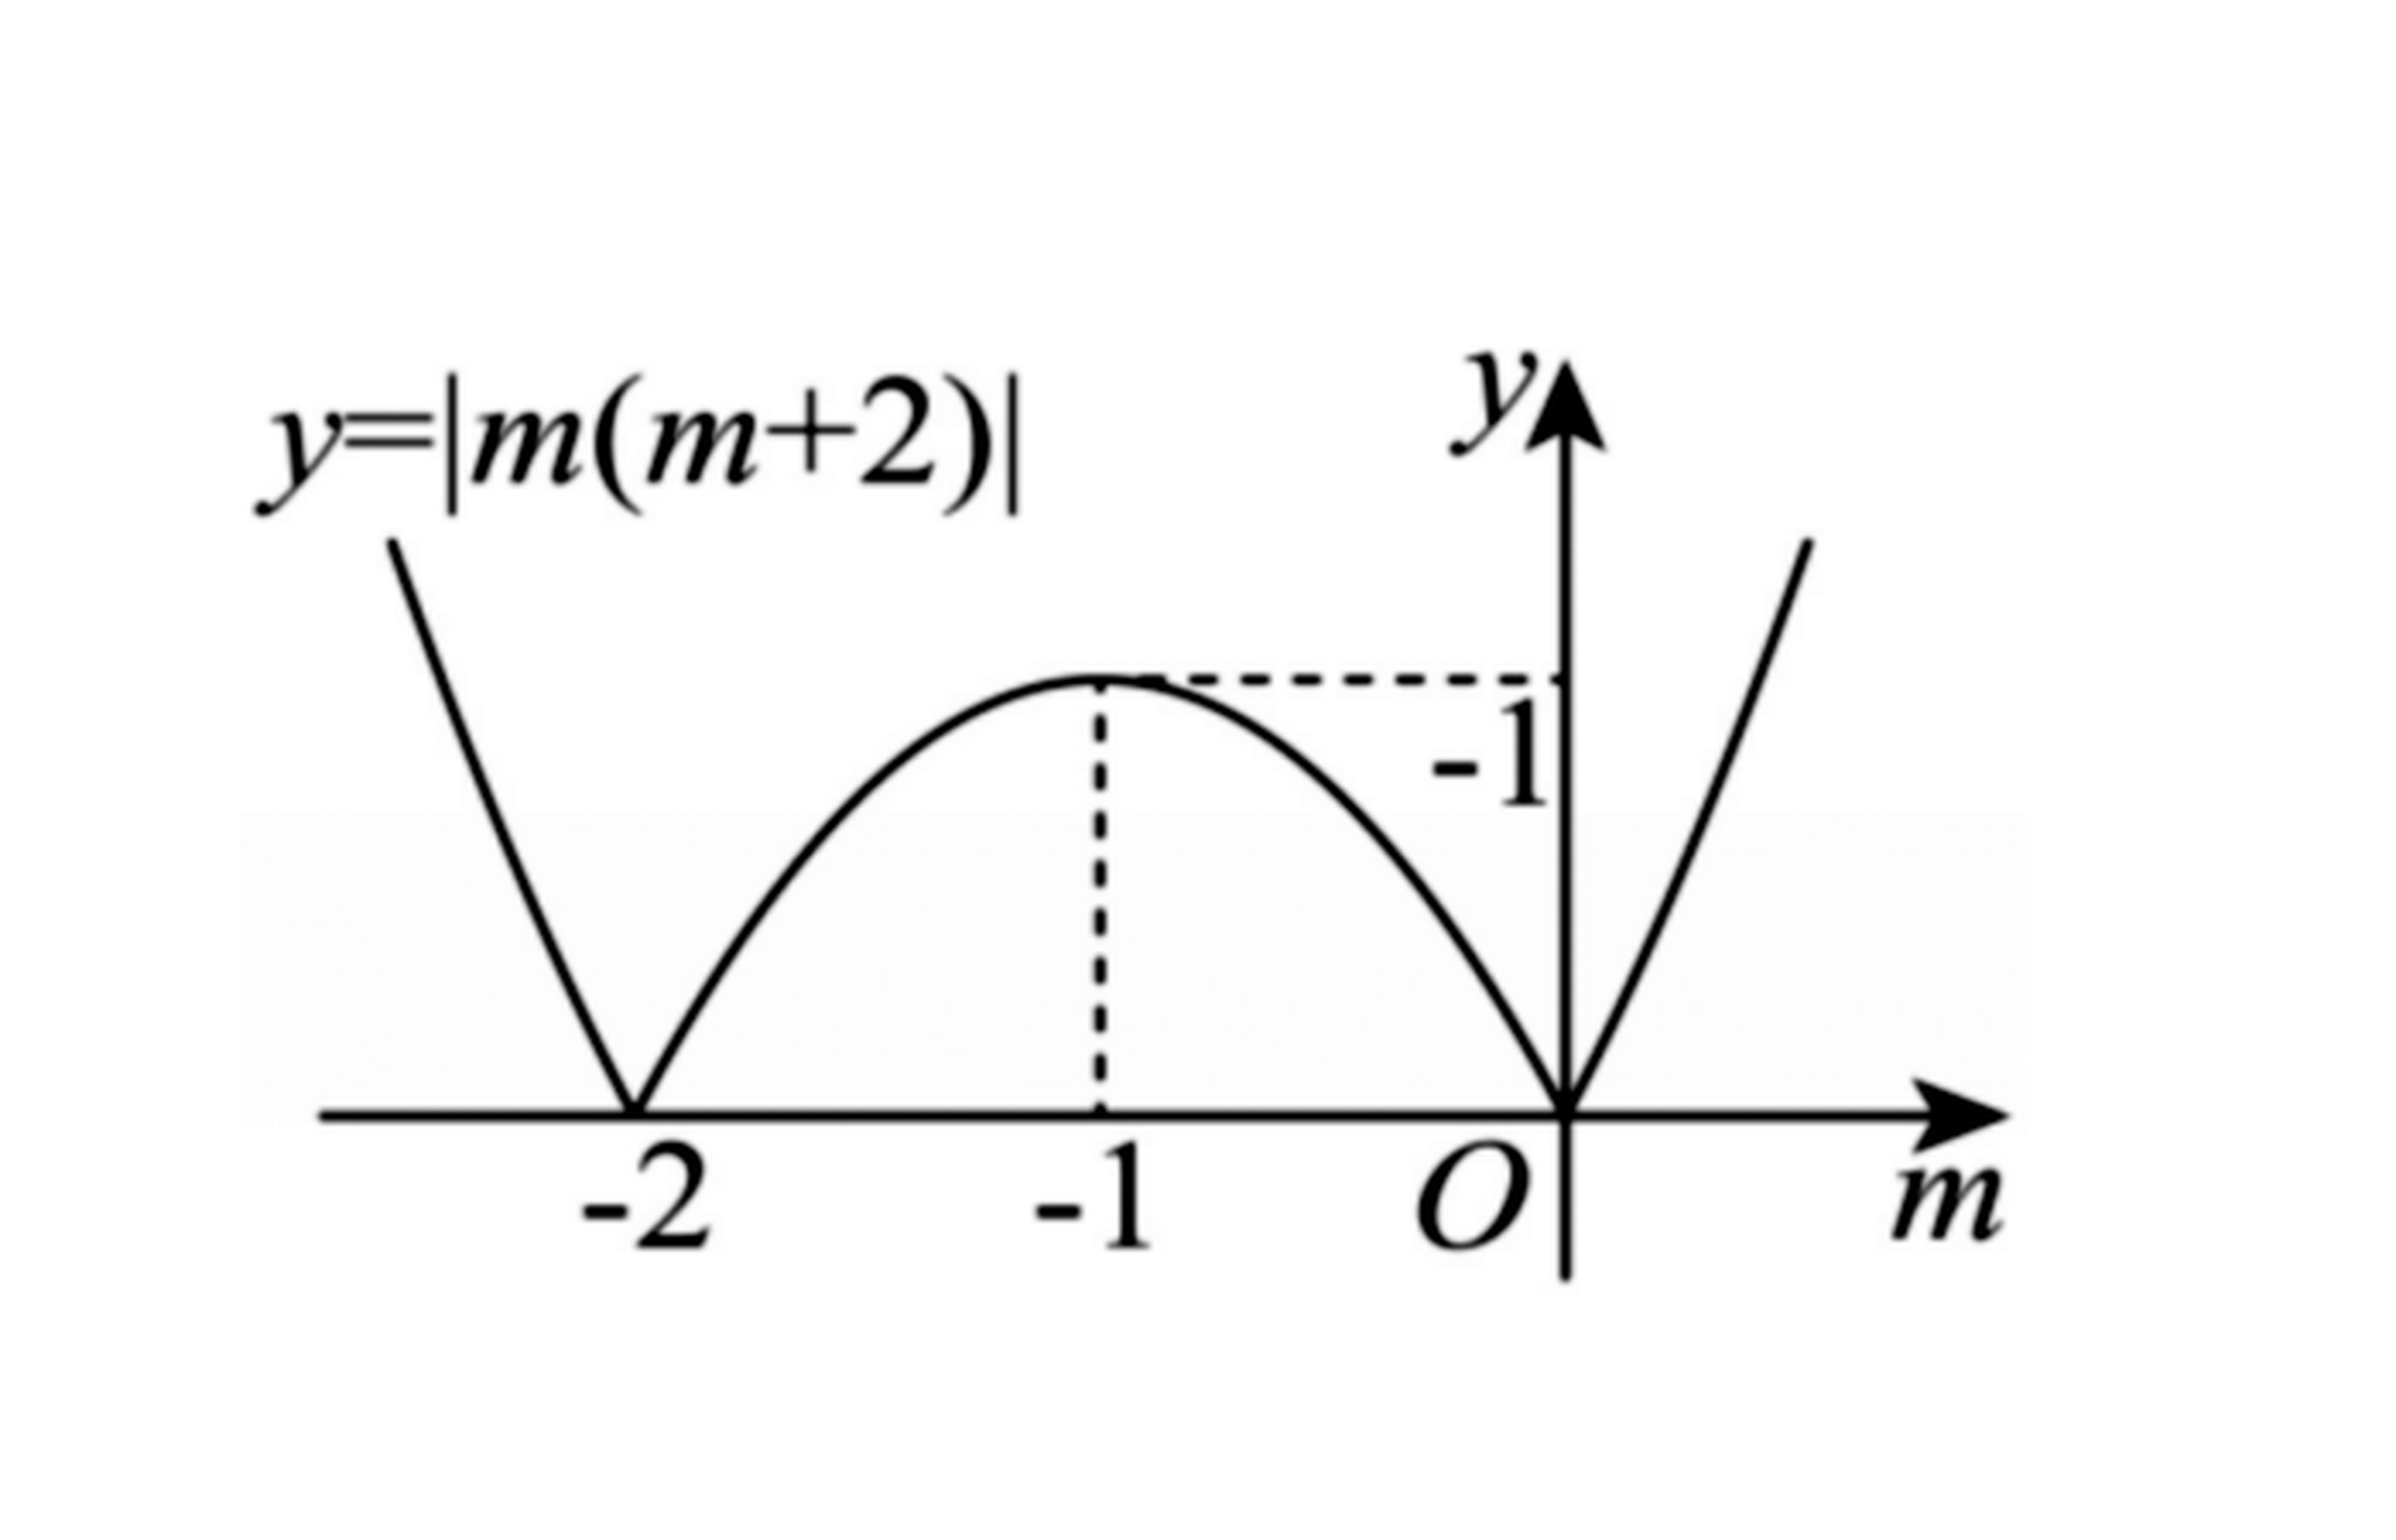
\includegraphics[width=0.46\textwidth]{figures/gao154_fujia2.png}
\end{center}
\step{由图像得 $k\in(0,1)$，}
\step{所以方程 $m^2+2m=k$ 和 $m^2+2m=-k$ 各有两个不同的根，}
\step{其中方程 $m^2+2m-k=0$ 的两根为 $m=-1\pm\sqrt{1+k}$，}
\step{方程 $m^2+2m+k=0$ 的两根为 $m=-1\pm\sqrt{1-k}$，}
\step{所以 $m_1=-1-\sqrt{1+k}$，$m_2=-1-\sqrt{1-k}$，$m_3=-1+\sqrt{1-k}$，$m_4=-1+\sqrt{1+k}$，且 $m_1<m_2<m_3<m_4$，}
\step{由 $m=\log_2 x$，则 $x=2^m$，}
\step{所以 $a=2^{-1-\sqrt{1+k}}$，$b=2^{-1-\sqrt{1-k}}$，$c=2^{-1+\sqrt{1-k}}$，$d=2^{-1+\sqrt{1+k}}$，}
\step{所以 $ad=2^{-1-\sqrt{1+k}}\times2^{-1+\sqrt{1+k}}=2^{(-1-\sqrt{1+k})+(-1+\sqrt{1+k})}=2^{-2}=\dfrac14$，}
\step{$b+c=2^{-1-\sqrt{1-k}}+2^{-1+\sqrt{1-k}}=\dfrac{2^{-\sqrt{1-k}}+2^{\sqrt{1-k}}}{2}$，}
\step{令 $s=\sqrt{1-k}$，其中 $s\in(0,1)$，则 $b+c=\dfrac12\left(2^{-s}+2^s\right)$，}
\step{设函数 $y=2^s+\dfrac1{2^s}$，令 $r=2^s\in(1,2)$，所以 $y=r+\dfrac1r$ 在 $(1,2)$ 上严格增，}
\step{所以函数 $y=2^s+\dfrac1{2^s}$ 在 $(0,1)$ 上严格增，所以 $y=2^s+\dfrac1{2^s}\in\left(2,\dfrac52\right)$，}
\step{所以 $b+c=\dfrac{2^{-s}+2^s}{2}\in\left(1,\dfrac54\right)$，$ad(b+c)=\dfrac{b+c}{4}\in\left(\dfrac14,\dfrac5{16}\right)$，}
\step{所以 $ad(b+c)$ 的取值范围是 $\left(\dfrac14,\dfrac5{16}\right)$，故选 $A$.}
\solend
\fi

\end{enumerate}

\end{document}
"
% 紧凑版：xelatex "\def\iscompact{1}% 高一154_徐汇中学_期中.tex
%   —— 高一上数学"2026-2027 年徐汇中学高一上期中"（试卷版/答案版/紧凑版）
% 试卷版：xelatex 高一154_徐汇中学_期中.tex
% 答案版：xelatex "\def\isanswer{1}\input{高一154_徐汇中学_期中.tex}"
% 紧凑版：xelatex "\def\iscompact{1}\input{高一154_徐汇中学_期中.tex}"
%
% ① 原始材料：微信公众号"魔都数学加油站"文章，连载"27学年高一154"，原文标题
% "27学年高一154——2026-2027年上海市徐汇中学高一上期中"；
% 原文链接：https://mp.weixin.qq.com/s/Qs2T7Zwsug-KKFE2wefDUg 。
% 正文为 12 张 PNG 页（01/03/04/05/07/11/12 为 2560×3620，
% 02/06/08/09/10 为 4762×6735，同一篇各页分辨率混排，逐页按各自分辨率裁图核对）。
% 体例：讲评版——一、填空题 3—12（10 题）、二、选择题 13—16（4 题）、
% 三、解答题 17—21（5 题）、附加题 1—2（2 题，原卷**另起编号**"1." "2."，
% 不与正题连号，同 高一a 成例），共 21 题；全卷每题均印【解析】
% （逐题核实，见 ② ②）。题目、答案、解析均据原图转录；卷面粉红色水印
% "魔都数学加油站"及公众号页脚未录入。
% 全卷插图清单（逐页通读 12 页确认）：3 组——
%   · Q15 题干配图（$f(x)=(x-a)(x-b)$ 抛物线，04 页右下：x/y 轴、O、1、
%     开口向上两零点均在 (0,1) 内），三版都出，裁 figures/gao154_q15_stem.png；
%   · Q15 四幅图像选项（05 页上半 2×2 排布，A/B/C/D 四幅指数函数图像，
%     合并成一张，照 高一136 Q13/Q22 成例），三版都出，
%     裁 figures/gao154_q15_opts.png；
%   · 附加题第 2 题解析配图（$y=\lvert m(m+2)\rvert$ 图像，11 页右上：
%     W 形折线、$-2$、$-1$、O、虚线 $y=1$ 与 $m=-1$），仅答案版出，
%     裁 figures/gao154_fujia2.png；
%   3 图均取自原卷截图，去粉色水印、去色、4× LANCZOS 放大；Q15 题干图
%   左侧题干残字"的图"已裁白。其余各页逐页确认无其它题目配图、无表格；
%   12 页下半仅水印、无正文。
%
% 卷首标题：原卷印作"2026-2027 年徐汇中学高一上期中"，年份区间按全稿惯例排 en dash；
% 原卷卷面未印副标题，本稿按同期中卷知识模块口径补出"集合与常用逻辑用语、不等式、函数"。
%
% ② 与原卷的排版差异：
%   ① 原文从第 3 题起，本稿保留原题号；共 21 题四节，正题到 21，附加题另起编号
%      1—2（\bigsec{附加题} 后 \begin{enumerate} 不 \setcounter，同 高一a 成例）；
%   ② 全 21 题均印【解析】、用 \solbegin…\solend，无只印【答案】或答案印括号内的题；
%      四道正题选择题答案在解析末句"故选 C／A／B／C"（Q13—Q16）、附加题第 2 题
%      答案在解析末句"故选 A"，括号 \mbox{（\quad）} 留空、不另提 \ans{}；
%      答案版【答案】/【解析】标记数 = 21 = 全卷题数；
%   ③ 原卷卷面未印副标题，本稿按知识模块口径补出；
%   ④ 原卷填空横线按全稿惯例排 \blankline[4.4em]；选择题括号排 \mbox{（\quad）}、
%      四道正题选择题与附加题第 2 题的选项段前按惯例各加 \keepwithprev
%      （Q15 与附加题 2 的选项段是整块图，\keepwithprev 后接 \begin{center}）；
%      解答题不留作答区、不加 \anspace（原卷为讲评版）；
%   ⑤ 数集黑板粗体：Q4"$x,y\in R$"、Q9"$x\in\R$"、Q13 无、
%      Q15"定义域 $\R$"、Q19"$\forall x\in\R$"、Q21"$x\in\N$"与"$k\in\N^*$"、
%      Q20"$a,b\in\R$"、附加题 2 无——原卷印斜体或正体粗体 R/N/N*，
%      按全稿惯例归一 \R／\N／\N^*；绝对值排 \lvert…\rvert
%      （Q5、Q9、Q12、Q13、Q16、Q21、附加题 2），集合描述竖线排 \mid
%      （Q5、Q17、Q19、Q21），不等号按全稿惯例排 \leqslant／\geqslant；
%      空集 \varnothing（Q21 题干 (3)）；
%   ⑥ 子集符号逐处照录、不得统一：Q6 题干印"$\{1,2\}\subset M\subseteq\{1,2,3,4,5\}$"
%      （前单线 ⊂、后带下划线 ⊆，同句两形并用），解析亦两形并用；
%      Q17 解析 (2)"$B\subset A$"印单线 ⊂；Q21 题干 (3)"$A\subseteq\{x\mid\cdots\}$"
%      印带下划线 ⊆——逐处放大核，分别 \subset／\subseteq，照录未统一（见 ④）；
%   ⑦ 判别式 Δ/△：Q18 解析 (1)"$\Delta=m^2-4(4m^2-3)$"与 Q19 解析 (1)
%      "$\Delta=4m^2-8m<0$"两处均印等腰偏高粗三角、照录 \Delta；本卷无扁等边
%      细线 \triangle 用例（见 ④）；
%   ⑧ 中文弯引号照录：Q4"设 $x$、$y\in\R$. 若 $x+y>2$，则 $x>1$ 或 $y>1$"、
%      附加题 1"$n$ 元集和集"与"3 元集和集"；注释里一律 ASCII 引号；
%      数学式内 CJK 用 \text{}（Q5 解集描述"或"、Q19 集合描述的"或"）；
%   ⑨ "图像／图象"逐处放大核：Q15 题干与解析印"图象"（象，无亻）、
%      Q16 无、附加题 2 解析印"图象"与"图像"（"画出函数…的图象"、
%      "由图像得"——两形并用，逐处照录未统一）；Q13/Q14 无数集图像字样；
%      半角逗号在数学组之间是全稿惯例、非笔误，逐处照录（Q3、Q10、Q16、
%      Q18、Q20、Q21 的 $x_1,x_2$ 之类）；行末西文句点 ASCII `.`；
%      行中全角逗号／顿号照录（Q6"3，4，5"、Q20"（单位：元）"、
%      附加题 1"$a_1,a_2,a_3,a_4$"）；
%   ⑩ 复杂式照录别简化：Q3 $a^{\frac{12}{7}}\cdot\left(\frac17\right)^{\frac17}
%      \cdot\sqrt[7]{a^4}$ 与 $7^{-\frac17}a^{\frac{16}{7}}$、Q7 $x^{-m}$、
%      Q8 $\frac{b-2a+2}{2a}$、Q11 $\frac{9+4\sqrt2}{6}$、Q12 $506\frac29$ 与
%      $506\frac49$、Q16 高斯取整 $[a]$、Q20 $c(x)=10x+\frac1{100}x^2$ 与
%      $q(x)=a+\frac xb$、Q21 $A^+$／$A^-$ 与 $|A^+|\geqslant2k-1$、
%      附加题 2 $m=-1\pm\sqrt{1+k}$ 与 $ad(b+c)$；
%      \left…\right 不得拆到不同 $…$ 组（Q5 $\left\{x\mid\cdots\right\}$、
%      Q20 $\left(\frac1b-\frac1{100}\right)$、附加题 2 $\left(\frac14,\frac5{16}\right)$）；
%      cases 块一律 \begin{cases}…\end{cases}；
%   ⑪ 一条 \step = 原卷解析的一个印刷行，cases 块整体算一个印刷行；别并折行、
%      别拆行。Q11 九行、Q12 六行、Q16 十六行、Q20 十一行、Q21 十七行、
%      附加题 2 十八行均按印刷行逐条断，不丢行；
%   ⑫ 配图：Q15 题干小图（三版都出）放 \item 内题干之后 \begin{center}，
%      Q15 四幅选项图（三版都出）放 \keepwithprev 之后的 \begin{center}，
%      Q15 用 \needvspace 守卫把"题干＋两图"整块推走（守卫放 \item 之前，
%      见 高一145 Q14/Q20 与 高一136 Q13 成例）；附加题 2 解析配图（仅答案版出）
%      放 \ifanswer 内 \solbegin…\solend 的 \step 之间（高一73 第 16 题成例）；
%   ⑬ 原卷解析内无红色"法一／法二"之类小标题，故本卷无 \stepm；红色水印
%      "魔都数学加油站"不录入；
%   ⑭ 跨页续印按题合并：见 ⑥；
%
% ③ 行数复核：一条 \step = 原卷解析的一个印刷行，cases 块作一个印刷行计。
%   逐题数（主会话逐页核对定稿）：Q3：1；Q4：1；Q5：3；Q6：4；Q7：3；
%   Q8：1；Q9：5；Q10：4；Q11：9；Q12：6；Q13：5；Q14：4；Q15：3；
%   Q16：16；Q17：5；Q18：9；Q19：10；Q20：11；Q21：17；
%   附加题 1：6；附加题 2：18。
%   合计 141 条 \step（本卷无 \stepm），与原卷逐题印刷行相等。全卷 21 题
%   均设 \solbegin…\solend，答案版【答案】/【解析】标记数 = 21 = 全卷题数。
%
% ④ 判别式／子集符号结论（逐处放大原图照录、不得统一，主会话像素级复核）：
%   判别式：Q18 解析 (1)"$\Delta=m^2-4(4m^2-3)=-15m^2+12\geqslant0$"、
%      Q19 解析 (1)"$\Delta=4m^2-8m<0$"共 2 处，逐处放大确认印等腰偏高
%      粗三角（高>宽、右斜边粗），照录 \Delta；本卷无扁等边细线 \triangle
%      用例，无几何三角形符号。
%   子集：Q6 题干"$\{1,2\}\subset M\subseteq\{1,2,3,4,5\}$"前 ⊂ 单线、
%      后 ⊆ 带下划线（/tmp/gao154/z/zoom/q6_subset.png），解析两处同样两形
%      并用，分别照录 \subset／\subseteq；Q17 解析 (2)"$B\subset A$"单线
%      照录 \subset；Q21 题干 (3)"$A\subseteq\{x\mid\cdots\}$"带下划线
%      照录 \subseteq。本卷 ⊂ 与 ⊆ 混用逐处照录、不得统一。
%      空集 \varnothing（Q21 题干 (3)）、数集 \R／\N／\N^* 归一见 ② ⑤。
%
% ⑤ 存疑照录（放大原图确认，照录未改、正文对应处另有 % 注）：
%   1. Q7 题干印 $f(x)=(3m-1)x^{-m}$，解析首句却写"幂函数 $f(x)=x^\alpha$
%      的系数必须为 1"（用 $\alpha$ 作指数记号），随后 $f(2)=2^\alpha=8$
%      得 $\alpha=3$、$f(x)=x^3$——题干指数 $-m$ 与解析 $\alpha$ 记法不同，
%      系原卷记号前后不一，逐处照录未统一（放大 01/02 页确认）。
%   2. Q11 解析"因为 $u>0,v>0$，由基本不等式得 $\frac{4v}{u}+\frac{2u}{v}
%      \geqslant2\sqrt{\frac{4v}{u}\cdot\frac{2u}{v}}=4\sqrt2$"与
%      "所以 $\frac4u+\frac1v=\frac16\left(\frac4u+\frac1v\right)(2u+v)$"
%      照录，未把 $u,v$ 化简回 $x,y$。
%   3. Q16 解析把"$[a]$ 表示不超过 $a$ 的最大整数"与"和至少有一个不小于 2"
%      连写在同一行（原卷如此），照录未改；末行"假设成立，C 正确，D 错误"照录。
%   4. Q18 解析 (2)"函数 $y=-7m^2+6$ 开口向下，对称轴为 $m=0$"却称求
%      "$y_{\min}$"（实为在 $m^2\leqslant\frac45$ 闭区间上的最小值），
%      照录未改。
%   5. Q20 题干"$q(x)=a+\frac xb$（$a,b\in\R$）"与解析
%      "$W(x)=\left(\frac1b-\frac1{100}\right)x^2+(a-10)x-160000$"照录；
%      末行解得 $a=90,b=\frac{500}{3}$ 照录未化简。
%   6. Q21 题干 (3)"$A\subseteq\{x\mid0\leqslant x\leqslant2020,x\in\N\}$"
%      与解析"$3k-1\leqslant2a_k+1\leqslant4041$（$k\in\N^*$）"照录；
%      末行"集合 $A$ 中元素的个数的最大值是 1347"照录。
%   7. 附加题 1 解析"相加化简得 $a_1+a_2+a_3+a_4=5$"照录；
%      附加题 2 解析"由图像得 $k\in(0,1)$"与"由图像得"／"的图象"两形
%      并用逐处照录（见 ② ⑨）；末行"$ad(b+c)$ 的取值范围是
%      $\left(\frac14,\frac5{16}\right)$，故选 A"照录。
%   全卷除此 7 类外未发现其它笔误／自相矛盾处；21 题均印【解析】、
%   无只印【答案】或答案印括号内的题（见 ② ②）。
%
% ⑥ 跨页续印按题合并说明（逐页核实定稿）：Q3—Q5 题干＋解析在 01 页
%   （Q5 解析末 2 行续 01 页下半）；Q6、Q7 题干＋解析在 01 页下半
%   （Q7 解析余 2 行续 02 页顶）；Q8、Q9 题干＋解析在 02 页上半
%   （Q9 解析余 3 行续 02 页下半）；Q10 题干＋解析在 02 页下半；
%   Q11 题干＋解析前 6 行在 03 页上半、余 3 行续 03 页下半；
%   Q12 题干＋解析前 5 行在 03 页下半、末行续 04 页顶；"二、选择题"
%   标题与 Q13 题干＋选项＋解析在 04 页上半；Q14 题干＋选项＋解析、
%   Q15 题干＋题干配图在 04 页下半；Q15 四幅选项图＋解析、
%   Q16 题干＋选项＋解析首行在 05 页上半，Q16 解析余 12 行在
%   05 页下半—06 页上半；"三、解答题"标题与 Q17 题干＋两问＋解析
%   在 06 页下半；Q18 题干＋两问＋解析在 07 页上半—下半；
%   Q19 题干＋两问＋解析首行在 07 页下半，解析余 8 行在 08 页上半；
%   Q20 题干在 08 页下半，解析 (1) 4 行＋(2) 首 4 行在 08 页下半—09 页上半，
%   (2) 余 2 行在 09 页下半；Q21 题干＋三问＋解析 (1)(2) 4 行在
%   09 页下半—10 页上半，解析 (3) 余 12 行在 10 页上半—下半；
%   "附加题"标题与附加题 1 题干＋解析首 3 行在 10 页下半，
%   余 3 行续 11 页上半；附加题 2 题干＋选项＋解析前 3 行在 11 页上半，
%   解析配图＋余 12 行在 11 页下半—12 页上半，末行
%   "所以 $ad(b+c)$ 的取值范围是 $\left(\frac14,\frac5{16}\right)$，故选 A"
%   为全卷收尾（12 页下半仅水印、无正文）。
%   本稿按题连排，不丢行、不并折行；全卷末题为附加题第 2 题。
%
\documentclass[a4paper,11pt]{article}
\usepackage{common}

\begin{document}

\examtitlest[3]{2026--2027 年徐汇中学高一上期中}{集合与常用逻辑用语、不等式、函数}

\bigsec{一、填空题}

\begin{enumerate}
\setcounter{enumi}{2}

% === Q3 === 分数指数幂照录；解析 1 行
\item 已知 $a>0$，化简 $a^{\frac{12}{7}}\cdot\left(\dfrac17\right)^{\frac17}\cdot\sqrt[7]{a^4}=$\blankline[4.4em].

\ifanswer
\solbegin
\step{$a^{\frac{12}{7}}\cdot\left(\dfrac17\right)^{\frac17}\cdot\sqrt[7]{a^4}=a^{\frac{12}{7}}\cdot(7^{-1})^{\frac17}\cdot a^{\frac47}=7^{-\frac17}a^{\frac{16}{7}}$.}
\solend
\fi

% === Q4 === 反证法；中文弯引号照录；解析 1 行
\item 用反证法证明命题：“设 $x$、$y\in\R$. 若 $x+y>2$，则 $x>1$ 或 $y>1$”时，假设的内容应该是\blankline[4.4em].

\ifanswer
\solbegin
\step{由反证法得，假设的内容应该是 $x\leqslant1$ 且 $y\leqslant1$.}
\solend
\fi

% === Q5 === 分式不等式；cases 块；解析 3 行
\item 不等式 $\dfrac{2x+3}{x-1}\geqslant1$ 的解集为\blankline[4.4em].

\ifanswer
\solbegin
\step{$\dfrac{2x+3}{x-1}\geqslant1$，即 $\dfrac{2x+3}{x-1}-1\geqslant0$，$\dfrac{x+4}{x-1}\geqslant0$，}
\step{等价于 $\begin{cases}(x+4)(x-1)\geqslant0\\x-1\ne0\end{cases}$，解得 $x>1$ 或 $x\leqslant-4$，}
\step{故解集为 $\{x\mid x>1\text{ 或 }x\leqslant-4\}$.}
\solend
\fi

% === Q6 === ⊂ 与 ⊆ 并用照录；解析 4 行
\item 满足条件 $\{1,2\}\subset M\subseteq\{1,2,3,4,5\}$ 的集合 $M$ 的个数为\blankline[4.4em].

\ifanswer
\solbegin
\step{因为 $\{1,2\}\subset M\subseteq\{1,2,3,4,5\}$，所以集合 $M$ 必含有元素 1，2，}
\step{且至少含有元素 3，4，5 中的一个，}
\step{则集合 $M$ 的个数与集合 $\{3,4,5\}$ 的非空子集的个数一样，}
\step{所以集合 $M$ 的个数为 $2^3-1=7$.}
\solend
\fi

% === Q7 === 题干 $x^{-m}$、解析用 $x^\alpha$ 记法，原卷记号差异照录（见 ⑤ 1）；解析 3 行
\item 已知幂函数 $f(x)=(3m-1)x^{-m}$，且 $f(2)=8$，则 $f(m)=$\blankline[4.4em].

\ifanswer
\solbegin
\step{幂函数 $f(x)=x^\alpha$ 的系数必须为 1，所以 $3m-1=1$，得 $m=\dfrac23$.}
\step{又 $f(2)=2^\alpha=8=2^3$，故 $\alpha=3$，即 $f(x)=x^3$，}
\step{所以 $f(m)=f\left(\dfrac23\right)=\left(\dfrac23\right)^3=\dfrac8{27}$.}
\solend
\fi

% === Q8 === 换底公式；解析 1 行
\item 已知 $a=\lg2$，$b=\lg3$，用含 $a,b$ 的代数式表示 $\log_4 75=$\blankline[4.4em].

\ifanswer
\solbegin
\step{$\log_4 75=\dfrac{\lg\left(3\times\frac{10^2}{2^2}\right)}{\lg2^2}=\dfrac{\lg3+2-2\lg2}{2\lg2}=\dfrac{b-2a+2}{2a}$.}
\solend
\fi

% === Q9 === 三角不等式取等；解析 5 行
\item 设 $x\in\R$，则方程 $\lvert x-2\rvert+\lvert3x+1\rvert=\lvert2x+3\rvert$ 的解集是\blankline[4.4em].

\ifanswer
\solbegin
\step{由 $\lvert x-2\rvert=\lvert2-x\rvert$，故原方程可化为 $\lvert2-x\rvert+\lvert3x+1\rvert=\lvert2x+3\rvert$，}
\step{又 $(2-x)+(3x+1)=2x+3$，}
\step{由三角不等式 $\lvert2-x\rvert+\lvert3x+1\rvert\geqslant\lvert(2-x)+(3x+1)\rvert=\lvert2x+3\rvert$，}
\step{当且仅当 $(2-x)(3x+1)\geqslant0$ 等号成立，}
\step{解 $(2-x)(3x+1)\geqslant0$ 得 $-\dfrac13\leqslant x\leqslant2$，故原方程的解集为 $\left[-\dfrac13,2\right]$.}
\solend
\fi

% === Q10 === 韦达定理；cases 块；解析 4 行
\item 已知一元二次不等式 $x^2+bx+c>0$ 的解集为 $(-\infty,-1)\cup(2,+\infty)$，则一元二次不等式 $bx^2+cx-1<0$ 的解集是\blankline[4.4em].

\ifanswer
\solbegin
\step{因为 $x^2+bx+c>0$ 的解集为 $(-\infty,-1)\cup(2,+\infty)$，}
\step{所以方程 $x^2+bx+c=0$ 的两根为 $-1$ 和 2，则有 $\begin{cases}-b=-1+2\\c=-1\times2\end{cases}$，即 $\begin{cases}b=-1\\c=-2\end{cases}$，}
\step{则 $bx^2+cx-1<0$ 等价于 $-x^2-2x-1<0$，得 $x^2+2x+1>0$，得 $(x+1)^2>0$，}
\step{解得 $x\ne-1$，故不等式 $bx^2+cx-1<0$ 的解集为 $(-\infty,-1)\cup(-1,+\infty)$.}
\solend
\fi

% === Q11 === 换元 $u,v$；解析 9 行
\item 已知正数 $x,y$ 满足 $2x+y=1$，则 $\dfrac4{x+2}+\dfrac1{y+1}$ 的最小值为\blankline[4.4em].

\ifanswer
\solbegin
\step{令 $u=x+2$，$v=y+1$，则 $u>2$，$v>1$，}
\step{且 $2u+v=2(x+2)+(y+1)=2x+y+5=6$.}
\step{因为 $u>0$，$v>0$，由基本不等式得 $\dfrac{4v}{u}+\dfrac{2u}{v}\geqslant2\sqrt{\dfrac{4v}{u}\cdot\dfrac{2u}{v}}=4\sqrt2$，}
\step{所以 $\dfrac4u+\dfrac1v=\dfrac16\left(\dfrac4u+\dfrac1v\right)(2u+v)=\dfrac16\left(9+\dfrac{4v}{u}+\dfrac{2u}{v}\right)\geqslant\dfrac{9+4\sqrt2}{6}$，}
\step{当且仅当 $\dfrac{4v}{u}=\dfrac{2u}{v}$，即 $u=\sqrt2v$ 时等号成立，}
\step{与 $2u+v=6$ 联立得 $u=\dfrac{6\sqrt2}{2\sqrt2+1}$，$v=\dfrac6{2\sqrt2+1}$，}
\step{此时 $x=u-2=\dfrac{2\sqrt2-2}{2\sqrt2+1}>0$，$y=v-1=\dfrac{5-2\sqrt2}{2\sqrt2+1}>0$，且 $2x+y=1$，}
\step{满足题设，所以下界可以取得，}
\step{因此 $\dfrac4{x+2}+\dfrac1{y+1}$ 的最小值为 $\dfrac{9+4\sqrt2}{6}$.}
\solend
\fi

% === Q12 === 2025 个整数解；解析 6 行
\item 若关于 $x$ 的不等式 $\lvert x-2k\rvert+\lvert x-3k\rvert<4k$ 共有 2025 个整数解，则实数 $k$ 的取值范围为\blankline[4.4em].

\ifanswer
\solbegin
\step{显然 $k>0$，由 $\lvert x-2k\rvert+\lvert x-3k\rvert<4k$，得 $\dfrac12k<x<\dfrac92k$，}
\step{因为该不等式共有 2025 个整数解，所以 $2024<\dfrac{9k}{2}-\dfrac k2\leqslant2026$，}
\step{解得 $506<k\leqslant506.5$，}
\step{由 $\dfrac k2\in(253,253.25]$，得这 2025 个整数解只能为 254、255、256、$\cdots$、2278，}
\step{所以 $2278<\dfrac{9k}{2}\leqslant2279$，解得 $506\dfrac29<k\leqslant506\dfrac49$，结合 $506<k\leqslant506.5$，}
\step{得 $k$ 的取值范围是 $\left(506\dfrac29,506\dfrac49\right]$.}
\solend
\fi

\end{enumerate}

\bigsec{二、选择题}

\begin{enumerate}
\setcounter{enumi}{12}

% === Q13 === 四选项一行；解析 5 行，故选 C
\item 若 $a<b<0$，则下列不等式中不成立的是\mbox{（\quad）}

\keepwithprev
A. $a-b>a$\qquad B. $\dfrac1a>\dfrac1b$\qquad C. $a^3>b^3$\qquad D. $\lvert a\rvert>\lvert b\rvert$

\ifanswer
\solbegin
\step{A 选项，因为 $b<0$，所以 $-b>0$，不等式两边同加上 $a$ 得 $a-b>a$，故 A 正确；}
\step{B 选项，因为 $a<b<0$，所以 $ab>0$，不等式两边同除以 $ab$，则 $\dfrac1b<\dfrac1a<0$，故 B 正确；}
\step{C 选项，不妨设 $a=-2$，$b=-1$，则 $a^3=-8$，$b^3=-1$，故 $a^3<b^3$，故 C 错误；}
\step{D 选项，因为 $a<b<0$，所以 $-a>-b$，即 $\lvert a\rvert>\lvert b\rvert$，故 D 正确.}
\step{故选 $C$.}
\solend
\fi

% === Q14 === 选项两行两列；解析 4 行，故选 A
\item 设命题 $p:x^2-5x+4\ne0$，命题 $q:x\ne1$，则 $p$ 是 $q$ 的\mbox{（\quad）}条件

\keepwithprev
A. 充分不必要\qquad\qquad B. 必要不充分

C. 充要\qquad\qquad D. 既不充分也不必要

\ifanswer
\solbegin
\step{$p:x^2-5x+4\ne0\Leftrightarrow(x-1)(x-4)\ne0\Leftrightarrow x\ne1$ 且 $x\ne4$；$q:x\ne1$.}
\step{充分性：当 $x\ne1$ 且 $x\ne4$ 时，$x\ne1$，所以 $p\Rightarrow q$；}
\step{必要性：当 $x\ne1$ 时，若 $x=4$，此时 $p$ 不成立，即 $q\nRightarrow p$；}
\step{所以 $p$ 是 $q$ 的充分不必要条件，故选 $A$.}
\solend
\fi

% === Q15 === 题干配图（三版都出）+ 四幅图像选项（2×2 合并，三版都出）；守卫放 \item 之前；解析 3 行，故选 B
\needvspace{9cm}
\item 已知函数 $f(x)=(x-a)(x-b)$（$a<b$）的图象如图所示，则函数 $g(x)=a^x-b$ 的图象可能是\mbox{（\quad）}

\begin{center}
% 抛物线题干配图取 04 页右下，去粉色水印、去色、4× LANCZOS 放大；三版都出
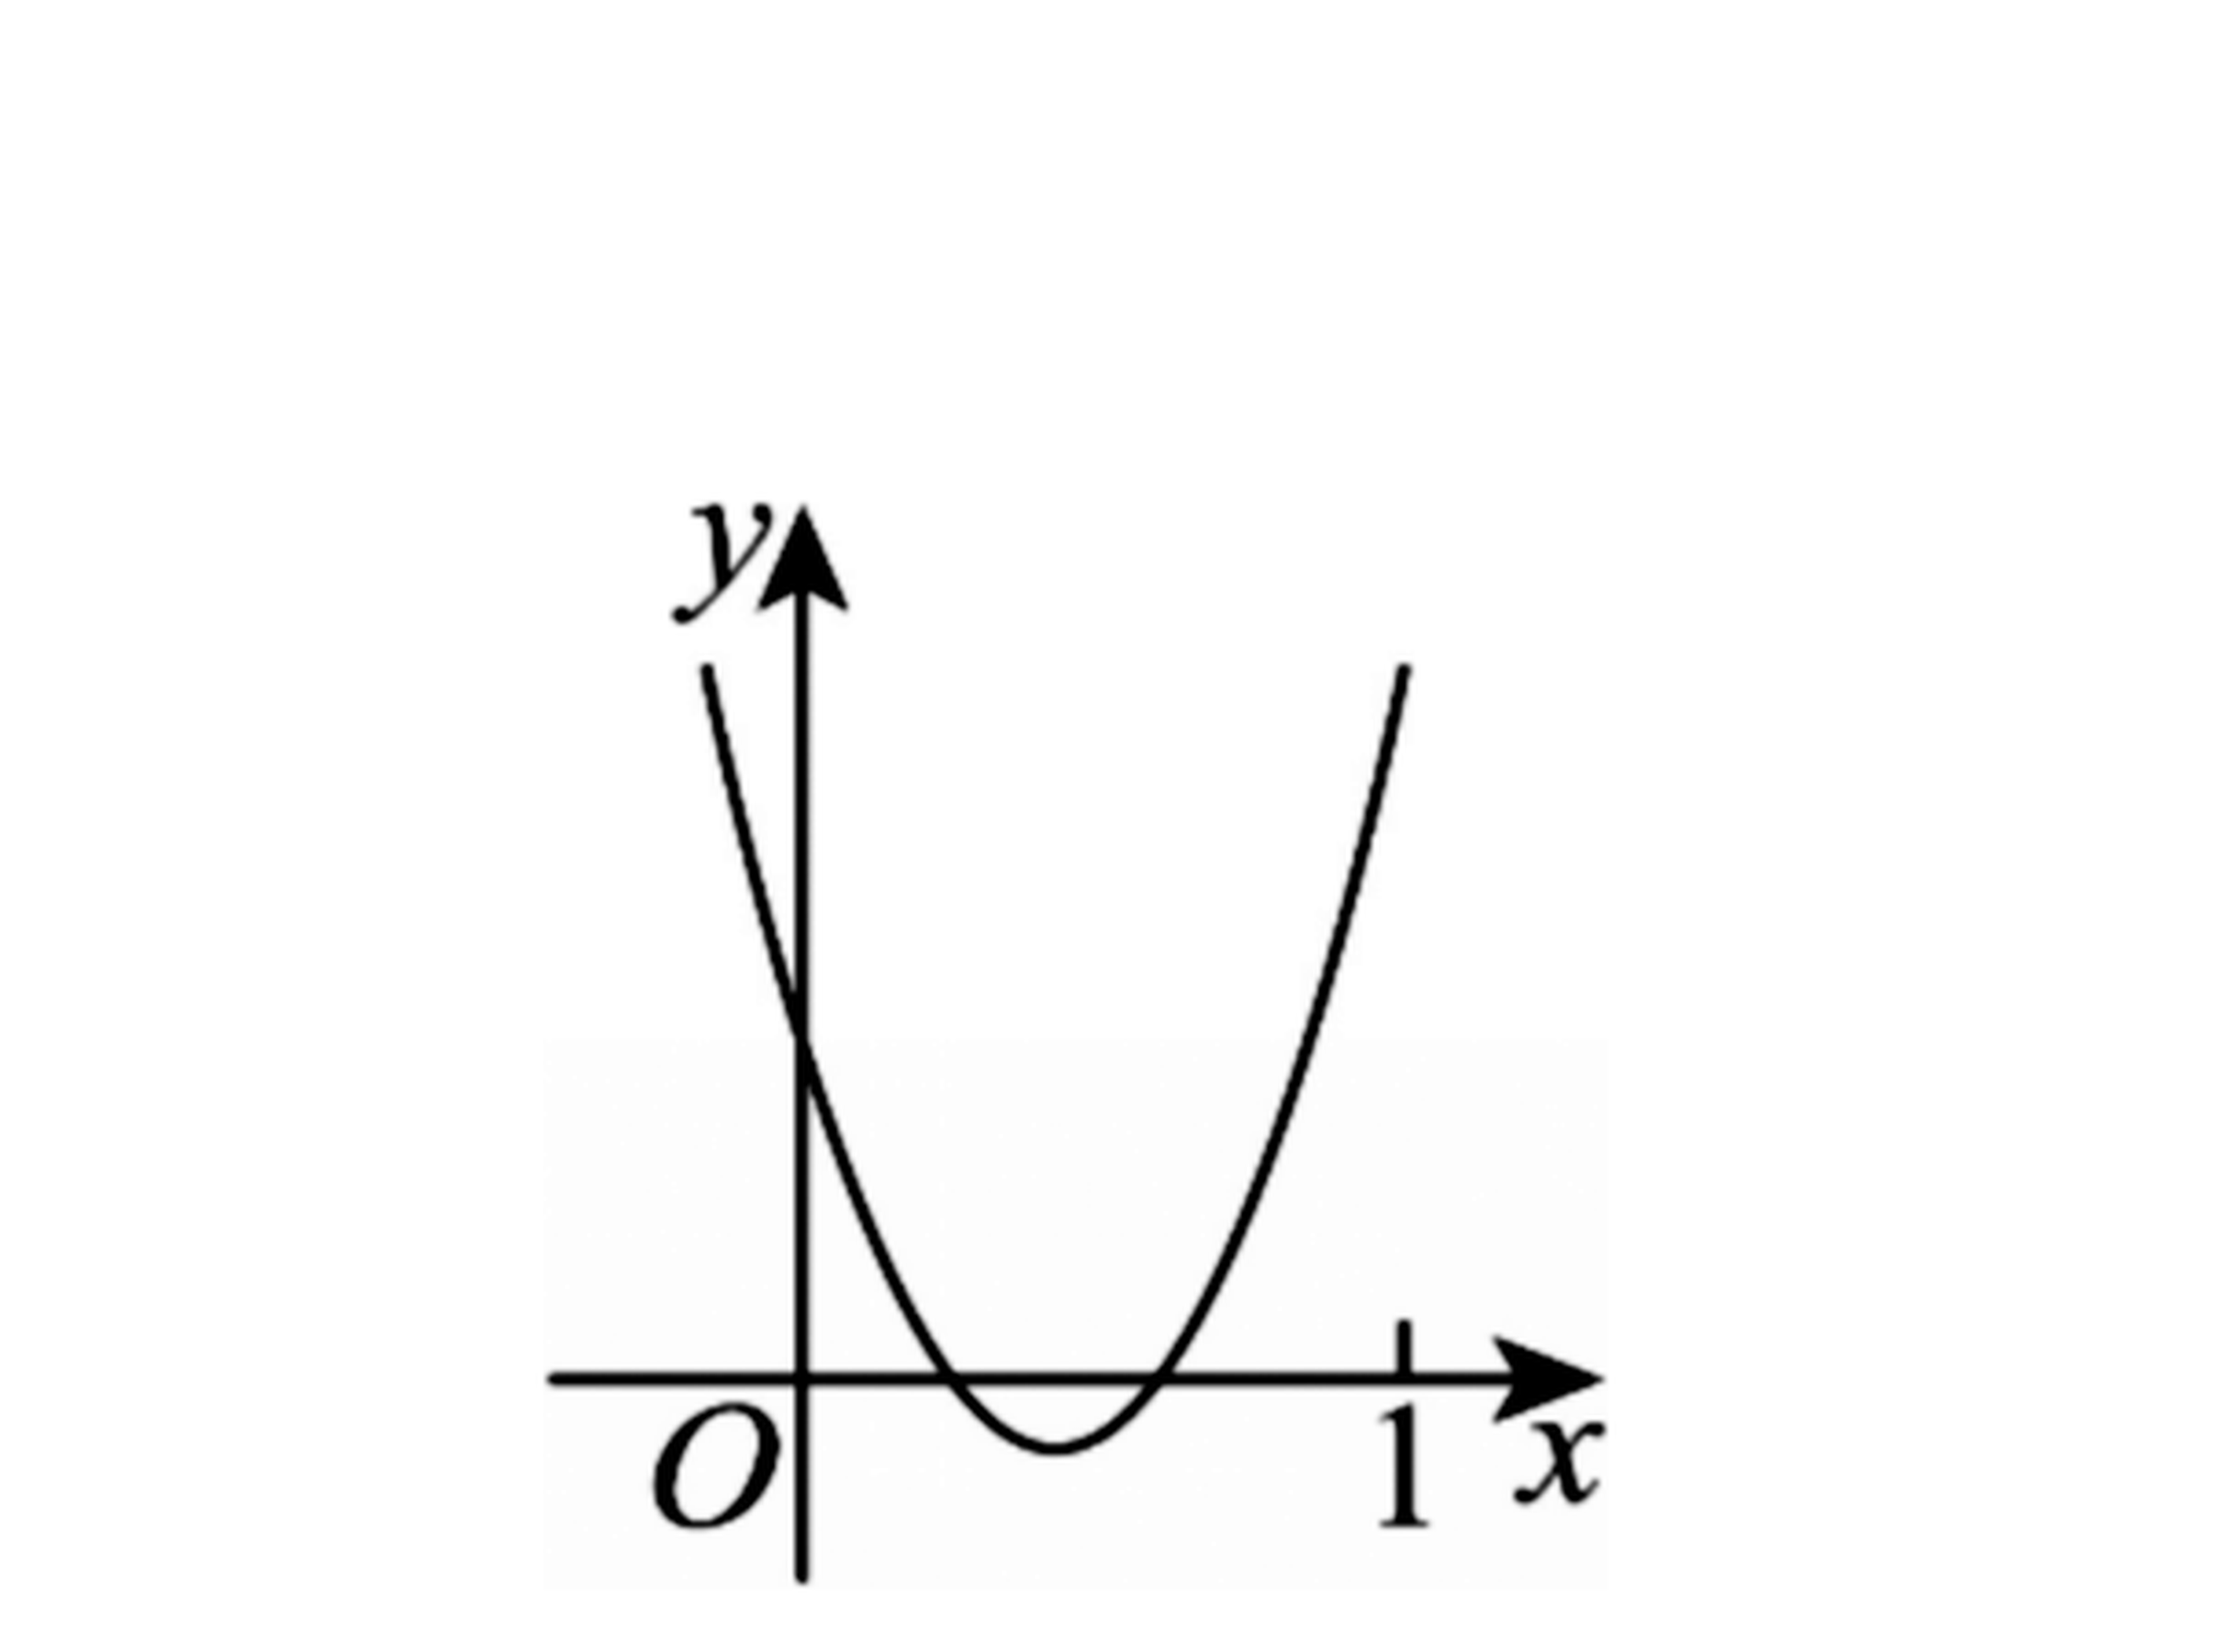
\includegraphics[width=0.32\textwidth]{figures/gao154_q15_stem.png}
\end{center}

\keepwithprev
\begin{center}
% 四幅指数函数图像选项取 05 页上半，按原卷 2×2 排布合并为一张，去粉色水印、去色、4× LANCZOS 放大；三版都出
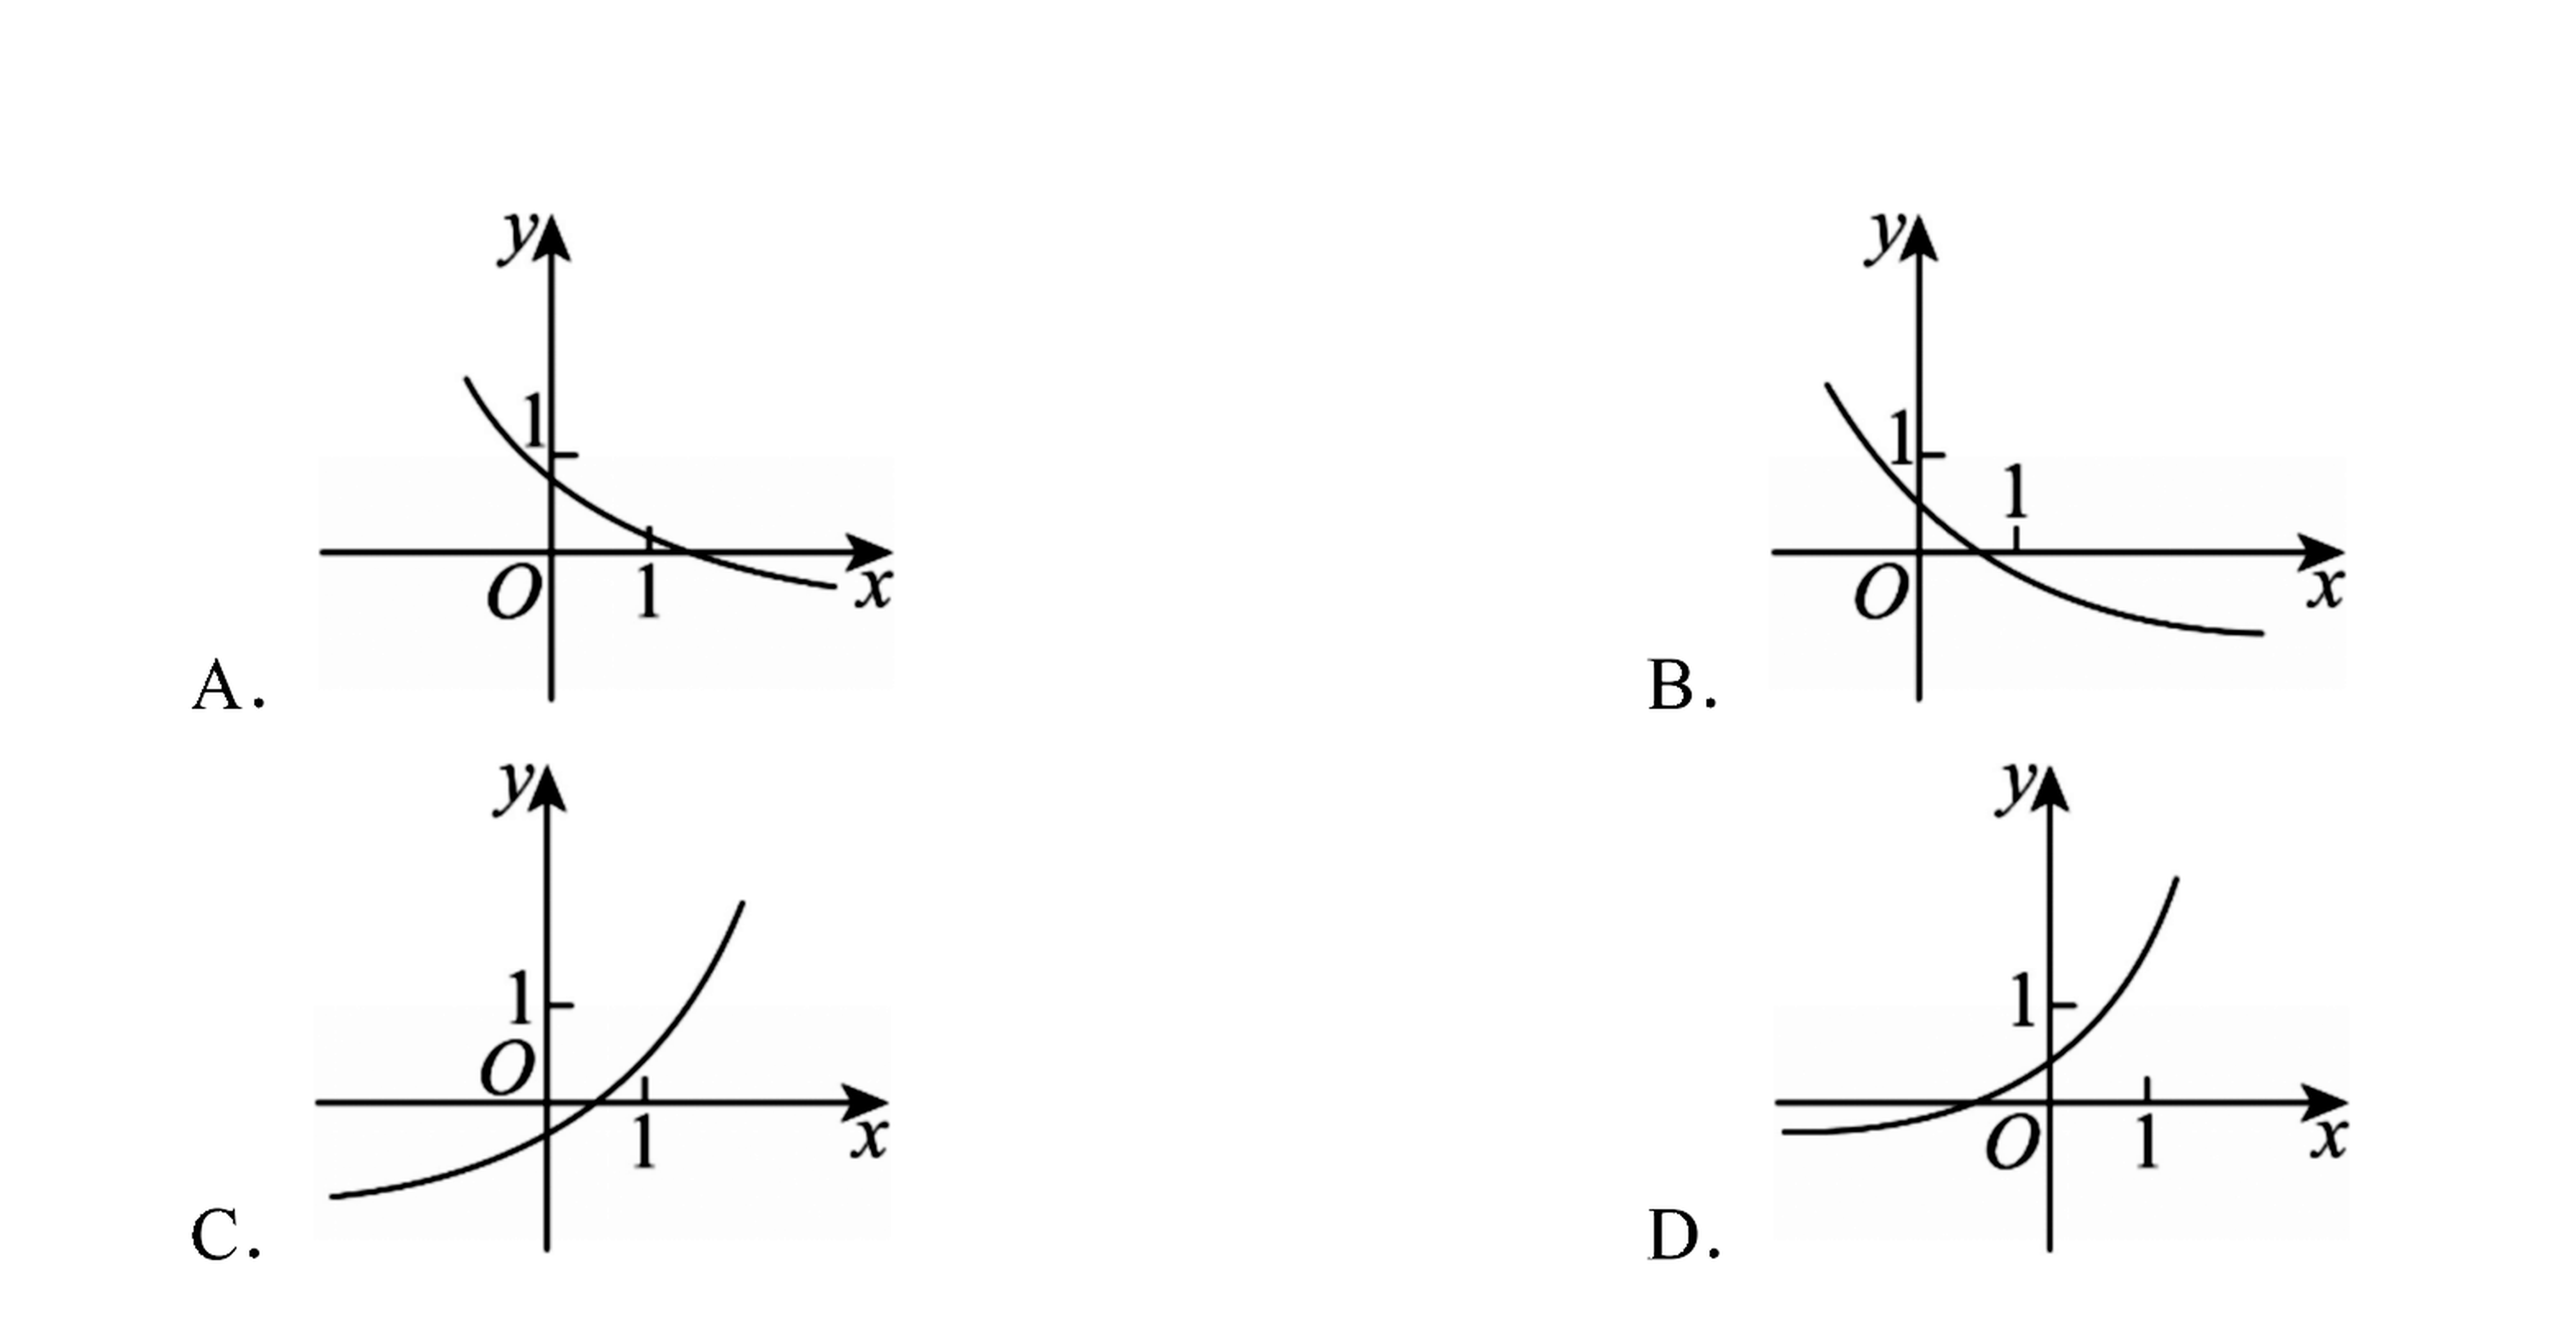
\includegraphics[width=0.80\textwidth]{figures/gao154_q15_opts.png}
\end{center}

\ifanswer
\solbegin
\step{由题意得 $0<a<b<1$，所以 $g(x)=a^x-b$ 在定义域 $\R$ 上严格减.}
\step{$g(0)=a^0-b=1-b>0$，$g(1)=a^1-b=a-b<0$，故 B 符合题意.}
\step{故选 $B$.}
\solend
\fi

% === Q16 === 高斯取整；解析 13 行，故选 C
\item 设 $[a]$ 表示不超过 $a$ 的最大整数，如 $[1.2]=1$，$[-3.2]=-4$，若 $x$、$y$、$z$ 为正实数，则 $\left[\dfrac{y+z}{x}\right]+\left[\dfrac{z+x}{y}\right]+\left[\dfrac{x+y}{z}\right]$ 的最小值为\mbox{（\quad）}

\keepwithprev
A. 2\qquad\qquad B. 3\qquad\qquad C. 4\qquad\qquad D. 6

\ifanswer
\solbegin
\step{若 $x$、$y$、$z$ 为正实数，}
\step{结合基本不等式得 $\dfrac{y+z}{x}+\dfrac{z+x}{y}+\dfrac{x+y}{z}=\dfrac yx+\dfrac xy+\dfrac zx+\dfrac xz+\dfrac zy+\dfrac yz$}
\step{$\geqslant2\sqrt{\dfrac yx\cdot\dfrac xy}+2\sqrt{\dfrac zx\cdot\dfrac xz}+2\sqrt{\dfrac zy\cdot\dfrac yz}=6$，当且仅当 $x=y=z$ 时取等号，}
\step{即 $\dfrac{y+z}{x}$，$\dfrac{z+x}{y}$，$\dfrac{x+y}{z}$ 中至少有一个不小于 2，不妨设 $\dfrac{y+z}{x}\geqslant\dfrac{z+x}{y}\geqslant\dfrac{x+y}{z}$，}
\step{$[a]$ 表示不超过 $a$ 的最大整数和 $\dfrac{y+z}{x}$，$\dfrac{z+x}{y}$，$\dfrac{x+y}{z}$ 中至少有一个不小于 2，}% 原卷此行把两句连写，照录未改（见 ⑤ 3）
\step{得 $\left[\dfrac{y+z}{x}\right]\geqslant2$，所以 $\left[\dfrac{y+z}{x}\right]+\left[\dfrac{z+x}{y}\right]+\left[\dfrac{x+y}{z}\right]\geqslant2$，}
\step{假设 $\left[\dfrac{y+z}{x}\right]+\left[\dfrac{z+x}{y}\right]+\left[\dfrac{x+y}{z}\right]$ 的最小值为 2，$\left[\dfrac{y+z}{x}\right]=2$，$\left[\dfrac{z+x}{y}\right]+\left[\dfrac{x+y}{z}\right]=0$，}
\step{所以 $2\leqslant\dfrac{y+z}{x}<3$，$0<\dfrac{z+x}{y}<1$，$0<\dfrac{x+y}{z}<1$，所以 $2<\dfrac{y+z}{x}+\dfrac{z+x}{y}+\dfrac{x+y}{z}<5$，}
\step{与 $\dfrac{y+z}{x}+\dfrac{z+x}{y}+\dfrac{x+y}{z}\geqslant6$ 矛盾，假设不成立，A 错误；}
\step{假设 $\left[\dfrac{y+z}{x}\right]+\left[\dfrac{z+x}{y}\right]+\left[\dfrac{x+y}{z}\right]$ 的最小值为 3，}
\step{则 $\left[\dfrac{y+z}{x}\right]=2$，$\left[\dfrac{z+x}{y}\right]=1$，$\left[\dfrac{x+y}{z}\right]=0$ 或 $\left[\dfrac{y+z}{x}\right]=3$，$\left[\dfrac{z+x}{y}\right]=\left[\dfrac{x+y}{z}\right]=0$，}
\step{同理可得 $3<\dfrac{y+z}{x}+\dfrac{z+x}{y}+\dfrac{x+y}{z}<6$，显然不成立，B 错误；}
\step{假设 $\left[\dfrac{y+z}{x}\right]+\left[\dfrac{z+x}{y}\right]+\left[\dfrac{x+y}{z}\right]$ 的最小值为 4，易得 $4<\dfrac{y+z}{x}+\dfrac{z+x}{y}+\dfrac{x+y}{z}<7$，}
\step{若取 $x=100$，$y=103$，$z=104$，则 $\left[\dfrac{y+z}{x}\right]=2$，$\left[\dfrac{z+x}{y}\right]=1$，$\left[\dfrac{x+y}{z}\right]=1$，}
\step{即 $\left[\dfrac{y+z}{x}\right]+\left[\dfrac{z+x}{y}\right]+\left[\dfrac{x+y}{z}\right]=4$，假设成立，C 正确，D 错误.}
\step{故选 $C$.}
\solend
\fi

\end{enumerate}

\bigsec{三、解答题}

\begin{enumerate}
\setcounter{enumi}{16}

% === Q17 === $B\subset A$ 单线照录；cases 块；解析 5 行
\item 设集合 $A=\{x\mid x^2+2x-3<0\}$，集合 $B=\{x\mid\lvert x+a\rvert<1\}$.

(1) 若 $a=3$，求 $A\cup B$；

(2) 设命题 $p:x\in A$，命题 $q:x\in B$，若 $p$ 是 $q$ 成立的必要不充分条件，求实数 $a$ 的取值范围.

\ifanswer
\solbegin
\step{(1) $A=(-3,1)$，}
\step{当 $a=3$ 时，$\lvert x+3\rvert<1$，解得 $-4<x<-2$，所以 $B=(-4,-2)$，}
\step{所以 $A\cup B=(-4,1)$.}
\step{(2) 因为 $p$ 是 $q$ 成立的必要不充分条件，所以 $B\subset A$.}
\step{因为 $A=(-3,1)$，$B=(-a-1,-a+1)$，所以 $\begin{cases}-a-1\geqslant-3\\-a+1<1\end{cases}$ 或 $\begin{cases}-a-1>-3\\-a+1\leqslant1\end{cases}$，解得 $0\leqslant a\leqslant2$.}
\solend
\fi

% === Q18 === 判别式 \Delta 两处照录；解析 9 行
\item 已知关于 $x$ 的一元二次方程 $x^2-mx+4m^2-3=0$ 的两个实根分别为 $x_1,x_2$.

(1) 若 $x_1,x_2$ 满足 $x_1+x_2=x_1x_2$，求实数 $m$ 的值；

(2) 求 $x_1^2+x_2^2$ 的最小值.

\ifanswer
\solbegin
\step{(1) 由韦达定理 $x_1+x_2=m$，$x_1x_2=4m^2-3$，}
\step{$\Delta=m^2-4(4m^2-3)=-15m^2+12\geqslant0$，即 $m^2\leqslant\dfrac45$.}
\step{由 $x_1+x_2=x_1x_2$ 得 $m=4m^2-3$，即 $4m^2-m-3=0$，}
\step{解得 $m=1$ 或 $m=-\dfrac34$.}
\step{$m=1$ 时 $m^2=1>\dfrac45$，$\Delta<0$，舍去；}
\step{$m=-\dfrac34$ 时 $m^2=\dfrac9{16}<\dfrac45$，符合，故 $m=-\dfrac34$.}
\step{(2) $x_1^2+x_2^2=(x_1+x_2)^2-2x_1x_2=m^2-2(4m^2-3)=-7m^2+6$，}
\step{函数 $y=-7m^2+6$ 开口向下，对称轴为 $m=0$，}% 原卷此处称求「最小值」，实为闭区间 $m^2\le\frac45$ 上的最小值，照录未改（见 ⑤ 4）
\step{故 $y_{\min}=-7\cdot\dfrac45+6=-\dfrac{28}{5}+\dfrac{30}{5}=\dfrac25$.}
\solend
\fi

% === Q19 === 全称命题；cases 块；解析 9 行
\item 设命题 $p$：对任意 $x\in\R$，不等式 $2mx^2+2mx+1>0$ 恒成立，$q:m\in\{m\mid\log_2(m-1)<1\}$.

(1) 若 $p$ 为真命题，求实数 $m$ 的取值范围；

(2) 若命题 $p$、$q$ 有且只有一个是真命题，求实数 $m$ 的取值范围.

\ifanswer
\solbegin
\step{(1) 由 $p$ 为真命题，得 $\forall x\in\R$，不等式 $2mx^2+2mx+1>0$ 恒成立，}
\step{当 $m=0$ 时，$1>0$ 恒成立；}
\step{当 $m\ne0$ 时，$\begin{cases}2m>0\\\Delta=4m^2-8m<0\end{cases}$，解得 $0<m<2$；}
\step{综上，$0\leqslant m<2$，即 $m$ 的取值范围是 $[0,2)$；}
\step{(2) 若 $q$ 为真，则有 $\log_2(m-1)<1$，得 $0<m-1<2$，解得 $1<m<3$，}
\step{因此命题 $q:m\in\{m\mid1<m<3\}$，由 (1) 得命题 $p:\{m\mid0\leqslant m<2\}$，}
\step{而命题 $p$、$q$ 有且只有一个是真命题，}
\step{当 $p$ 真 $q$ 假时，$\begin{cases}0\leqslant m<2\\m\leqslant1\text{ 或 }m\geqslant3\end{cases}$，解得 $0\leqslant m\leqslant1$，}
\step{当 $p$ 假 $q$ 真时，$\begin{cases}m<0\text{ 或 }m\geqslant2\\1<m<3\end{cases}$，解得 $2\leqslant m<3$，}
\step{故实数 $m$ 的取值范围是 $\{m\mid0\leqslant m\leqslant1\text{ 或 }2\leqslant m<3\}$.}
\solend
\fi

% === Q20 === Labubu 成本题；解析 10 行
\item Labubu 公司拟在 2027 年初推出智能机器人系列玩偶（单位：套）. 根据以往经验，其中一条生产线每月生产 $x$ 套玩具的成本 $P$ 由两部分费用（单位：元）构成：

(i) 固定成本（与生产玩具套数 $x$ 无关），总计 160000 元；

(ii) 每生产 $x$ 套需另投入的生产成本 $c(x)$ 元，其中 $c(x)=10x+\dfrac1{100}x^2$.

(1) 假设该生产线每月生产出的玩具能全部售出，问：该生产线每月生产玩具多少套时，可使得平均每套所需成本费用最少？此时每套玩具的成本费用是多少？

(2) 假设该生产线每月生产出的玩具能全部售出，但随着 $x$ 的增大，每月生产所需的直接总成本在急剧增加，因此售价也需随着 $x$ 的增大而适当增加. 设每套玩具的售价为 $q(x)$ 元，$q(x)=a+\dfrac xb$（$a,b\in\R$）. 若当月产量为 10000 套时利润最大，此时每套售价为 150 元，试求 $a,b$ 的值.（利润=销售收入$-$成本费用）

\ifanswer
\solbegin
\step{(1) 每月总成本 $P=160000+10x+\dfrac1{100}x^2$，}
\step{平均每套成本为 $\dfrac Px=\dfrac{160000}{x}+10+\dfrac x{100}\geqslant10+2\sqrt{\dfrac{160000}{x}\cdot\dfrac x{100}}=90$.}
\step{等号成立当且仅当 $\dfrac{160000}{x}=\dfrac x{100}$ 时，即 $x=4000$ 时取等号，}
\step{所以每月生产 4000 套时平均每套成本最少，此时每套成本为 90 元.}
\step{(2) 利润 $W(x)=x\cdot q(x)-P=\left(\dfrac1b-\dfrac1{100}\right)x^2+(a-10)x-160000$.}
\step{要在 $x=10000$ 处取得最大值，需 $\dfrac1b-\dfrac1{100}<0$，且对称轴为 $x=10000$，}
\step{故 $-\dfrac{a-10}{2\left(\frac1b-\frac1{100}\right)}=10000$，即 $a-10=-20000\left(\dfrac1b-\dfrac1{100}\right)$.}
\step{又 $q(10000)=a+\dfrac{10000}{b}=150$.}
\step{令 $t=\dfrac1b$，则 $a=150-10000t$，}
\step{代入上式 $140-10000t=-20000t+200$，解得 $t=\dfrac3{500}$，即 $b=\dfrac{500}{3}$；}
\step{再由 $a=150-10000\times\dfrac3{500}=150-60=90$，所以 $a=90$，$b=\dfrac{500}{3}$.}
\solend
\fi

% === Q21 === $A^+$／$A^-$ 新定义；$A\subseteq$ 带下划线照录、\varnothing；解析 16 行
\item 设集合 $A$ 为非空数集，定义 $A^+=\{x\mid x=a+b,a,b\in A\}$，$A^-=\{x\mid x=\lvert a-b\rvert,a,b\in A\}$.

(1) 若集合 $A=\{-1,1\}$，写出集合 $A^+$ 及 $A^-$；

(2) 若集合 $A=\{x_1,x_2,x_3,x_4\}$，$x_1<x_2<x_3<x_4$，且 $A^-=A$，求证：$x_1+x_4=x_2+x_3$；

(3) 若集合 $A\subseteq\{x\mid0\leqslant x\leqslant2020,x\in\N\}$，且 $A^+\cap A^-=\varnothing$，求集合 $A$ 元素的个数的最大值.

\ifanswer
\solbegin
\step{(1) 由 $A=\{-1,1\}$，得 $A^+=\{-2,0,2\}$，$A^-=\{0,2\}$；}
\step{(2) 由于集合 $A=\{x_1,x_2,x_3,x_4\}$，$x_1<x_2<x_3<x_4$，且 $A^-=A$，}
\step{所以 $A^-$ 中也只包含四个元素，即 $A^-=\{0,x_2-x_1,x_3-x_1,x_4-x_1\}$，}
\step{剩下的 $x_3-x_2=x_4-x_3=x_2-x_1$，所以 $x_1+x_4=x_2+x_3$；}
\step{(3) 设 $A=\{a_1,a_2,\cdots,a_k\}$ 满足题意，其中 $a_1<a_2<\cdots<a_k$，}
\step{则 $2a_1<a_1+a_2<a_1+a_3<\cdots<a_1+a_k<a_2+a_k<a_3+a_k<\cdots<a_{k-1}+a_k<2a_k$，所以 $\lvert A^+\rvert\geqslant2k-1$，}
\step{且 $a_1-a_1<a_2-a_1<a_3-a_1<\cdots<a_k-a_1$，所以 $\lvert A^-\rvert\geqslant k$，}
\step{因为 $A^+\cap A^-=\varnothing$，所以 $\lvert A^+\cup A^-\rvert=\lvert A^+\rvert+\lvert A^-\rvert\geqslant3k-1$，}
\step{$A^+\cup A^-$ 中最小的元素为 0，最大的元素为 $2a_k$，所以 $\lvert A^+\cup A^-\rvert\leqslant2a_k+1$，}
\step{所以 $3k-1\leqslant2a_k+1\leqslant4041$（$k\in\N^*$），所以 $k\leqslant1347$，}
\step{实际上当 $A=\{674,675,676,\cdots,2020\}$ 时满足题意，证明如下：}
\step{设 $A=\{m,m+1,m+2,\cdots,2020\}$，$m\in\N$，}
\step{则 $A^+=\{2m,2m+1,2m+2,\cdots,4040\}$，$A^-=\{0,1,2,\cdots,2020-m\}$，}
\step{由题意得 $2020-m<2m$，即 $m>673\dfrac13$，}
\step{故 $m$ 的最小值为 674，于是当 $m=674$ 时，$A$ 中元素最多，}
\step{即 $A=\{674,675,676,\cdots,2020\}$ 时满足题意，}
\step{综上所述，集合 $A$ 中元素的个数的最大值是 1347.}
\solend
\fi

\end{enumerate}

\bigsec{附加题}

\begin{enumerate}

% === 附加题 1 === 另起编号 1；「n 元集和集」弯引号；解析 6 行
\item 设集合 $A=\{a_1,a_2,a_3,a_4\}$，$C=\{2,3,4,6\}$，新定义：集合 $A$ 中所有含 $n$ 个元素的子集中 $n$ 个元素之和的不同值组成的集合为“$n$ 元集和集”. 若 $A$ 的“3 元集和集”为 $C$，则集合 $A=$\blankline[4.4em].

\ifanswer
\solbegin
\step{集合 $A$ 的 3 元子集共有 4 个：$\{a_1,a_2,a_3\}$，$\{a_1,a_2,a_4\}$，$\{a_1,a_3,a_4\}$，$\{a_2,a_3,a_4\}$，}
\step{集合 $C=\{a_1+a_2+a_3,a_1+a_2+a_4,a_1+a_3+a_4,a_2+a_3+a_4\}$，}
\step{不妨令 $a_1<a_2<a_3<a_4$，}
\step{则 $a_1+a_2+a_3<a_1+a_2+a_4<a_1+a_3+a_4<a_2+a_3+a_4$，}
\step{而 $C=\{2,3,4,6\}$，因此 $\begin{cases}a_1+a_2+a_3=2\\a_1+a_2+a_4=3\\a_1+a_3+a_4=4\\a_2+a_3+a_4=6\end{cases}$，相加化简得 $a_1+a_2+a_3+a_4=5$，}
\step{解得 $a_1=-1$，$a_2=1$，$a_3=2$，$a_4=3$，所以 $A=\{-1,1,2,3\}$.}
\solend
\fi

% === 附加题 2 === 解析配图（仅答案版出）；四选项；解析 15 行，故选 A
\item 已知函数 $f(x)=\log_p x+q$，其中 $p>0$ 且 $p\ne1$，曲线 $y=f(x)$ 经过 $P(1,2)$、$Q(2,3)$ 两点. 设 $g(x)=f(x)\cdot[f(x)-2]$，若 $\lvert g(a)\rvert=\lvert g(b)\rvert=\lvert g(c)\rvert=\lvert g(d)\rvert$，且 $a<b<c<d$，则 $ad(b+c)$ 的取值范围为\mbox{（\quad）}

\keepwithprev
A. $\left(\dfrac14,\dfrac5{16}\right)$\qquad B. $\left(\dfrac18,\dfrac5{16}\right)$\qquad C. $\left(\dfrac14,\dfrac25\right)$\qquad D. $\left(\dfrac18,\dfrac25\right)$

\ifanswer
\solbegin
\step{函数 $f(x)=\log_p x+q$，且曲线 $y=f(x)$ 经过点 $P(1,2)$ 和 $Q(2,3)$，}
\step{所以 $\begin{cases}f(1)=q=2\\f(2)=\log_p2+q=3\end{cases}$，解得 $p=2$，$q=2$，$f(x)=\log_2 x+2$.}
\step{不妨设 $\lvert g(x)\rvert=k$，令 $\log_2 x=m$，则 $f(x)\cdot[f(x)-2]=m(m+2)=m^2+2m$，}
\step{画出函数 $y=\lvert m^2+2m\rvert$ 的图象，如图所示，}
\begin{center}
% $y=|m(m+2)|$ 图像取 11 页右上，去粉色水印、去色、4× LANCZOS 放大；仅答案版出
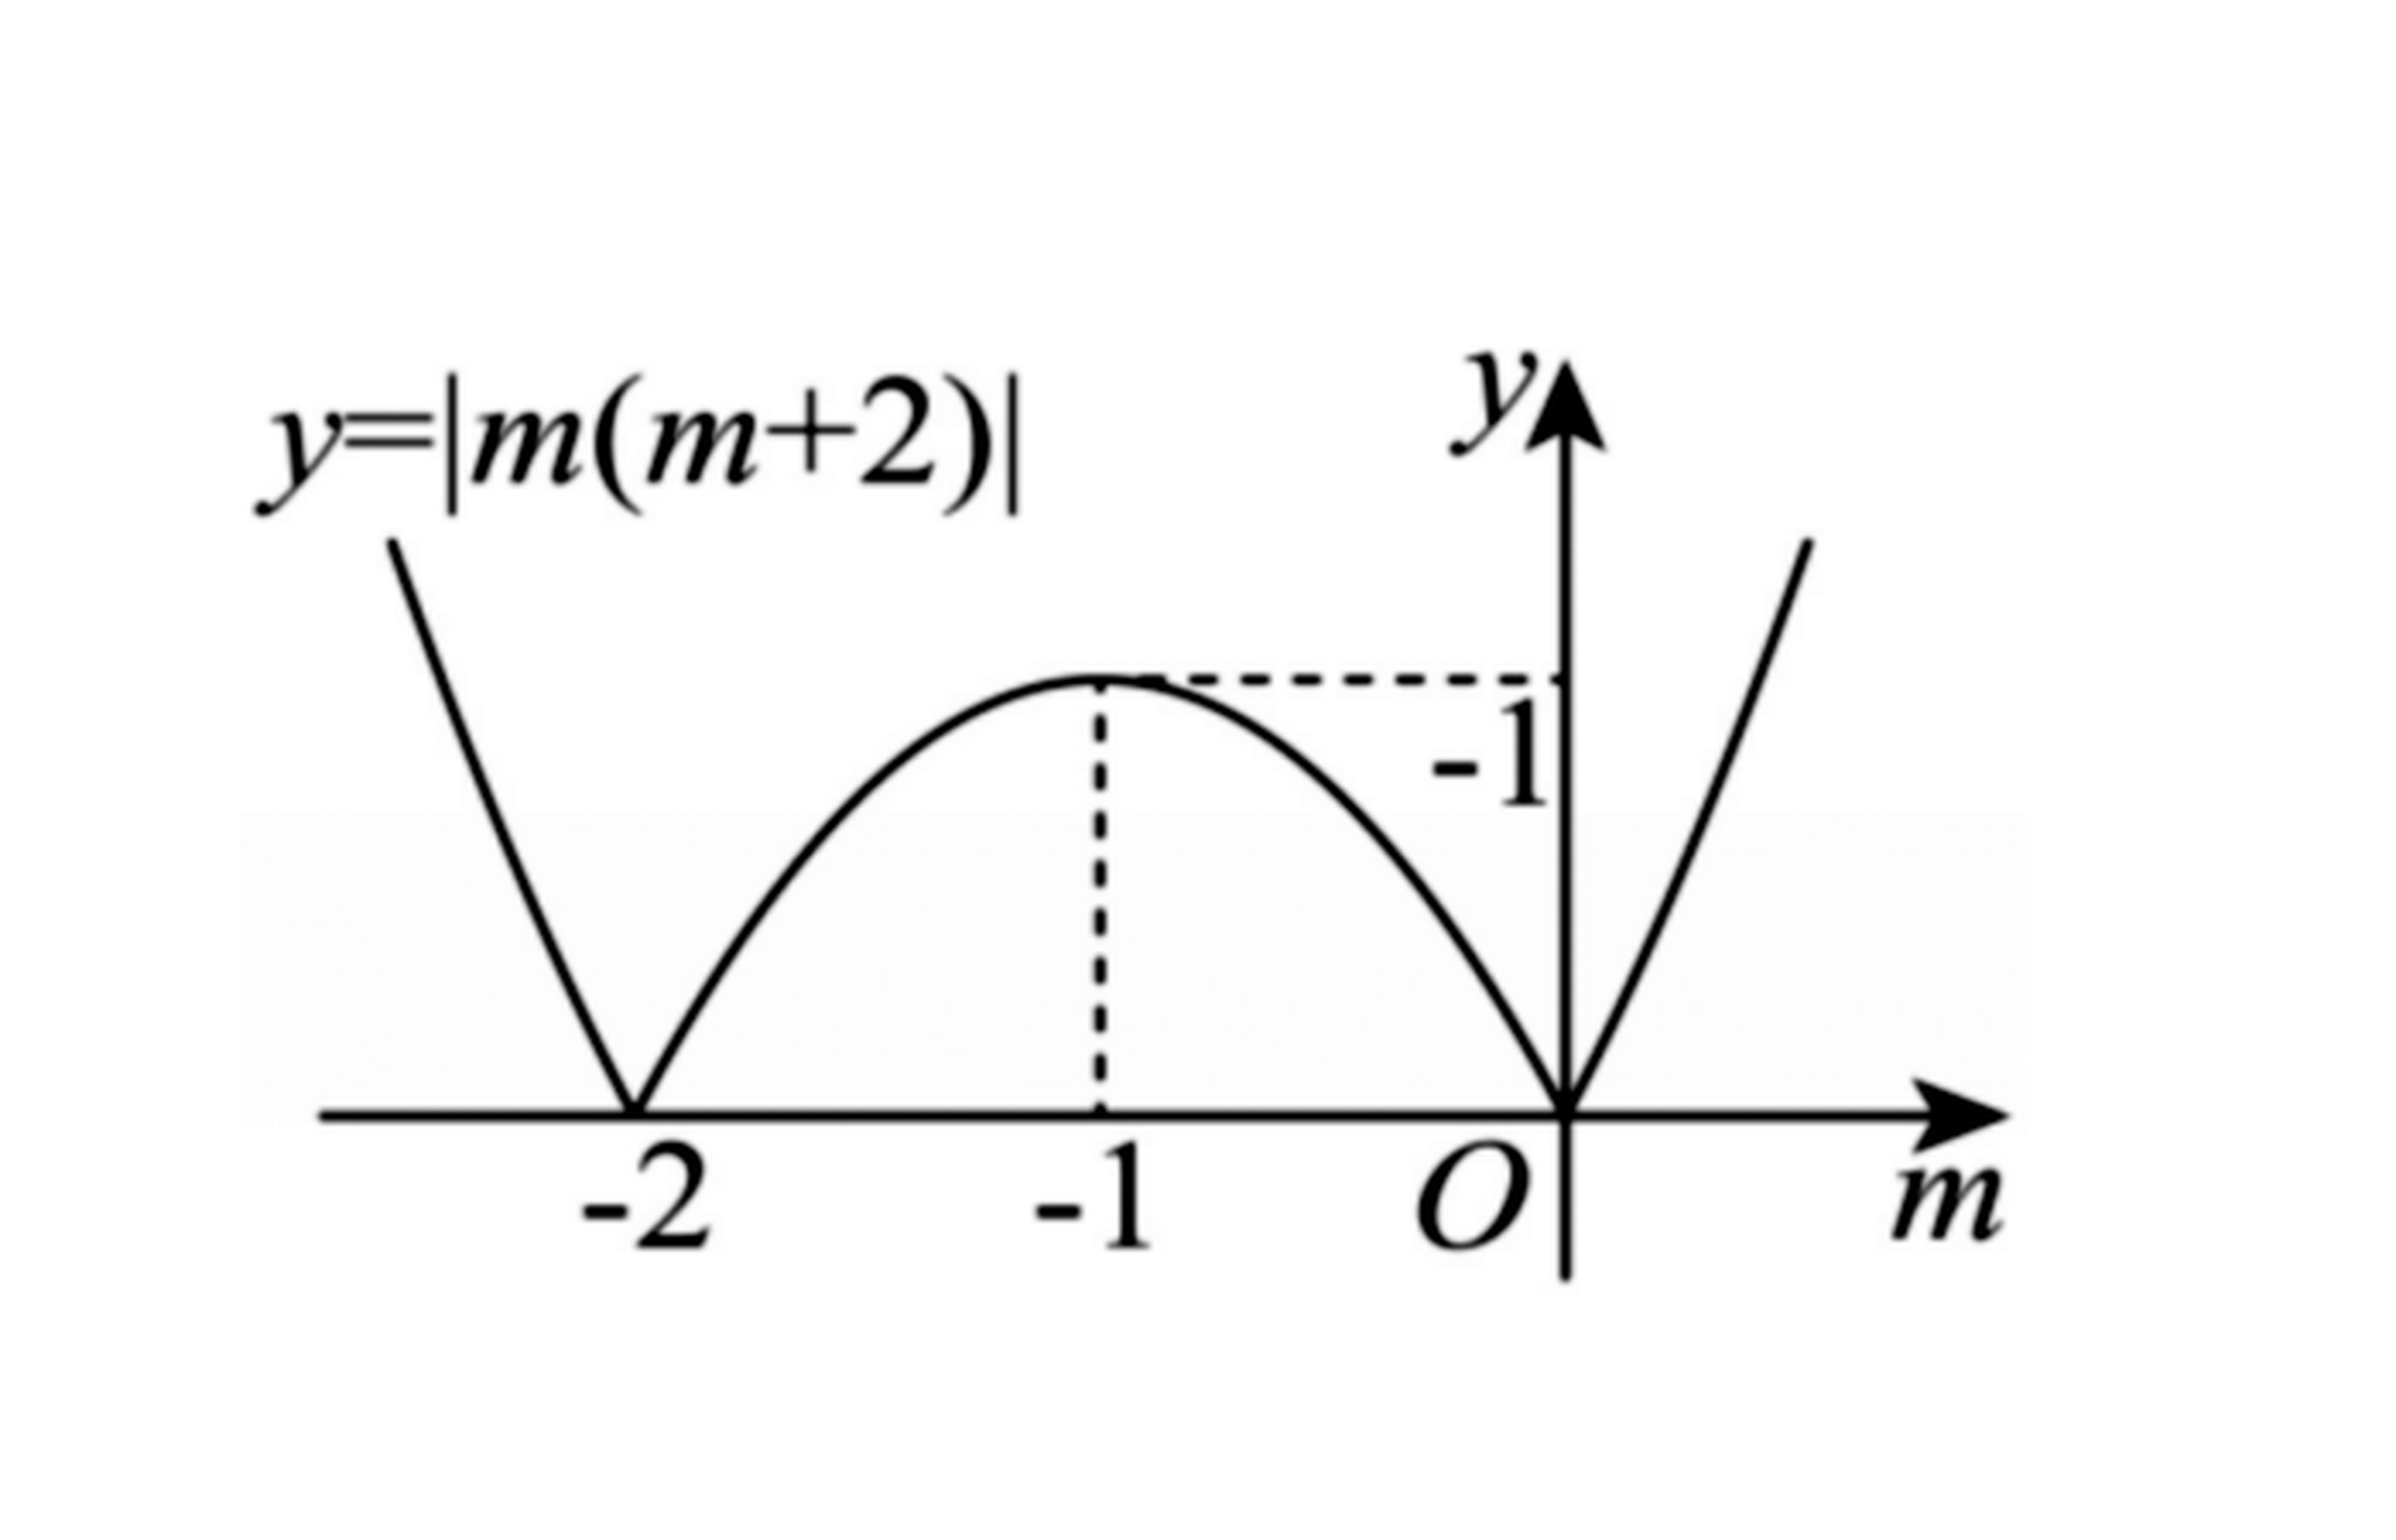
\includegraphics[width=0.46\textwidth]{figures/gao154_fujia2.png}
\end{center}
\step{由图像得 $k\in(0,1)$，}
\step{所以方程 $m^2+2m=k$ 和 $m^2+2m=-k$ 各有两个不同的根，}
\step{其中方程 $m^2+2m-k=0$ 的两根为 $m=-1\pm\sqrt{1+k}$，}
\step{方程 $m^2+2m+k=0$ 的两根为 $m=-1\pm\sqrt{1-k}$，}
\step{所以 $m_1=-1-\sqrt{1+k}$，$m_2=-1-\sqrt{1-k}$，$m_3=-1+\sqrt{1-k}$，$m_4=-1+\sqrt{1+k}$，且 $m_1<m_2<m_3<m_4$，}
\step{由 $m=\log_2 x$，则 $x=2^m$，}
\step{所以 $a=2^{-1-\sqrt{1+k}}$，$b=2^{-1-\sqrt{1-k}}$，$c=2^{-1+\sqrt{1-k}}$，$d=2^{-1+\sqrt{1+k}}$，}
\step{所以 $ad=2^{-1-\sqrt{1+k}}\times2^{-1+\sqrt{1+k}}=2^{(-1-\sqrt{1+k})+(-1+\sqrt{1+k})}=2^{-2}=\dfrac14$，}
\step{$b+c=2^{-1-\sqrt{1-k}}+2^{-1+\sqrt{1-k}}=\dfrac{2^{-\sqrt{1-k}}+2^{\sqrt{1-k}}}{2}$，}
\step{令 $s=\sqrt{1-k}$，其中 $s\in(0,1)$，则 $b+c=\dfrac12\left(2^{-s}+2^s\right)$，}
\step{设函数 $y=2^s+\dfrac1{2^s}$，令 $r=2^s\in(1,2)$，所以 $y=r+\dfrac1r$ 在 $(1,2)$ 上严格增，}
\step{所以函数 $y=2^s+\dfrac1{2^s}$ 在 $(0,1)$ 上严格增，所以 $y=2^s+\dfrac1{2^s}\in\left(2,\dfrac52\right)$，}
\step{所以 $b+c=\dfrac{2^{-s}+2^s}{2}\in\left(1,\dfrac54\right)$，$ad(b+c)=\dfrac{b+c}{4}\in\left(\dfrac14,\dfrac5{16}\right)$，}
\step{所以 $ad(b+c)$ 的取值范围是 $\left(\dfrac14,\dfrac5{16}\right)$，故选 $A$.}
\solend
\fi

\end{enumerate}

\end{document}
"
%
% ① 原始材料：微信公众号"魔都数学加油站"文章，连载"27学年高一154"，原文标题
% "27学年高一154——2026-2027年上海市徐汇中学高一上期中"；
% 原文链接：https://mp.weixin.qq.com/s/Qs2T7Zwsug-KKFE2wefDUg 。
% 正文为 12 张 PNG 页（01/03/04/05/07/11/12 为 2560×3620，
% 02/06/08/09/10 为 4762×6735，同一篇各页分辨率混排，逐页按各自分辨率裁图核对）。
% 体例：讲评版——一、填空题 3—12（10 题）、二、选择题 13—16（4 题）、
% 三、解答题 17—21（5 题）、附加题 1—2（2 题，原卷**另起编号**"1." "2."，
% 不与正题连号，同 高一a 成例），共 21 题；全卷每题均印【解析】
% （逐题核实，见 ② ②）。题目、答案、解析均据原图转录；卷面粉红色水印
% "魔都数学加油站"及公众号页脚未录入。
% 全卷插图清单（逐页通读 12 页确认）：3 组——
%   · Q15 题干配图（$f(x)=(x-a)(x-b)$ 抛物线，04 页右下：x/y 轴、O、1、
%     开口向上两零点均在 (0,1) 内），三版都出，裁 figures/gao154_q15_stem.png；
%   · Q15 四幅图像选项（05 页上半 2×2 排布，A/B/C/D 四幅指数函数图像，
%     合并成一张，照 高一136 Q13/Q22 成例），三版都出，
%     裁 figures/gao154_q15_opts.png；
%   · 附加题第 2 题解析配图（$y=\lvert m(m+2)\rvert$ 图像，11 页右上：
%     W 形折线、$-2$、$-1$、O、虚线 $y=1$ 与 $m=-1$），仅答案版出，
%     裁 figures/gao154_fujia2.png；
%   3 图均取自原卷截图，去粉色水印、去色、4× LANCZOS 放大；Q15 题干图
%   左侧题干残字"的图"已裁白。其余各页逐页确认无其它题目配图、无表格；
%   12 页下半仅水印、无正文。
%
% 卷首标题：原卷印作"2026-2027 年徐汇中学高一上期中"，年份区间按全稿惯例排 en dash；
% 原卷卷面未印副标题，本稿按同期中卷知识模块口径补出"集合与常用逻辑用语、不等式、函数"。
%
% ② 与原卷的排版差异：
%   ① 原文从第 3 题起，本稿保留原题号；共 21 题四节，正题到 21，附加题另起编号
%      1—2（\bigsec{附加题} 后 \begin{enumerate} 不 \setcounter，同 高一a 成例）；
%   ② 全 21 题均印【解析】、用 \solbegin…\solend，无只印【答案】或答案印括号内的题；
%      四道正题选择题答案在解析末句"故选 C／A／B／C"（Q13—Q16）、附加题第 2 题
%      答案在解析末句"故选 A"，括号 \mbox{（\quad）} 留空、不另提 \ans{}；
%      答案版【答案】/【解析】标记数 = 21 = 全卷题数；
%   ③ 原卷卷面未印副标题，本稿按知识模块口径补出；
%   ④ 原卷填空横线按全稿惯例排 \blankline[4.4em]；选择题括号排 \mbox{（\quad）}、
%      四道正题选择题与附加题第 2 题的选项段前按惯例各加 \keepwithprev
%      （Q15 与附加题 2 的选项段是整块图，\keepwithprev 后接 \begin{center}）；
%      解答题不留作答区、不加 \anspace（原卷为讲评版）；
%   ⑤ 数集黑板粗体：Q4"$x,y\in R$"、Q9"$x\in\R$"、Q13 无、
%      Q15"定义域 $\R$"、Q19"$\forall x\in\R$"、Q21"$x\in\N$"与"$k\in\N^*$"、
%      Q20"$a,b\in\R$"、附加题 2 无——原卷印斜体或正体粗体 R/N/N*，
%      按全稿惯例归一 \R／\N／\N^*；绝对值排 \lvert…\rvert
%      （Q5、Q9、Q12、Q13、Q16、Q21、附加题 2），集合描述竖线排 \mid
%      （Q5、Q17、Q19、Q21），不等号按全稿惯例排 \leqslant／\geqslant；
%      空集 \varnothing（Q21 题干 (3)）；
%   ⑥ 子集符号逐处照录、不得统一：Q6 题干印"$\{1,2\}\subset M\subseteq\{1,2,3,4,5\}$"
%      （前单线 ⊂、后带下划线 ⊆，同句两形并用），解析亦两形并用；
%      Q17 解析 (2)"$B\subset A$"印单线 ⊂；Q21 题干 (3)"$A\subseteq\{x\mid\cdots\}$"
%      印带下划线 ⊆——逐处放大核，分别 \subset／\subseteq，照录未统一（见 ④）；
%   ⑦ 判别式 Δ/△：Q18 解析 (1)"$\Delta=m^2-4(4m^2-3)$"与 Q19 解析 (1)
%      "$\Delta=4m^2-8m<0$"两处均印等腰偏高粗三角、照录 \Delta；本卷无扁等边
%      细线 \triangle 用例（见 ④）；
%   ⑧ 中文弯引号照录：Q4"设 $x$、$y\in\R$. 若 $x+y>2$，则 $x>1$ 或 $y>1$"、
%      附加题 1"$n$ 元集和集"与"3 元集和集"；注释里一律 ASCII 引号；
%      数学式内 CJK 用 \text{}（Q5 解集描述"或"、Q19 集合描述的"或"）；
%   ⑨ "图像／图象"逐处放大核：Q15 题干与解析印"图象"（象，无亻）、
%      Q16 无、附加题 2 解析印"图象"与"图像"（"画出函数…的图象"、
%      "由图像得"——两形并用，逐处照录未统一）；Q13/Q14 无数集图像字样；
%      半角逗号在数学组之间是全稿惯例、非笔误，逐处照录（Q3、Q10、Q16、
%      Q18、Q20、Q21 的 $x_1,x_2$ 之类）；行末西文句点 ASCII `.`；
%      行中全角逗号／顿号照录（Q6"3，4，5"、Q20"（单位：元）"、
%      附加题 1"$a_1,a_2,a_3,a_4$"）；
%   ⑩ 复杂式照录别简化：Q3 $a^{\frac{12}{7}}\cdot\left(\frac17\right)^{\frac17}
%      \cdot\sqrt[7]{a^4}$ 与 $7^{-\frac17}a^{\frac{16}{7}}$、Q7 $x^{-m}$、
%      Q8 $\frac{b-2a+2}{2a}$、Q11 $\frac{9+4\sqrt2}{6}$、Q12 $506\frac29$ 与
%      $506\frac49$、Q16 高斯取整 $[a]$、Q20 $c(x)=10x+\frac1{100}x^2$ 与
%      $q(x)=a+\frac xb$、Q21 $A^+$／$A^-$ 与 $|A^+|\geqslant2k-1$、
%      附加题 2 $m=-1\pm\sqrt{1+k}$ 与 $ad(b+c)$；
%      \left…\right 不得拆到不同 $…$ 组（Q5 $\left\{x\mid\cdots\right\}$、
%      Q20 $\left(\frac1b-\frac1{100}\right)$、附加题 2 $\left(\frac14,\frac5{16}\right)$）；
%      cases 块一律 \begin{cases}…\end{cases}；
%   ⑪ 一条 \step = 原卷解析的一个印刷行，cases 块整体算一个印刷行；别并折行、
%      别拆行。Q11 九行、Q12 六行、Q16 十六行、Q20 十一行、Q21 十七行、
%      附加题 2 十八行均按印刷行逐条断，不丢行；
%   ⑫ 配图：Q15 题干小图（三版都出）放 \item 内题干之后 \begin{center}，
%      Q15 四幅选项图（三版都出）放 \keepwithprev 之后的 \begin{center}，
%      Q15 用 \needvspace 守卫把"题干＋两图"整块推走（守卫放 \item 之前，
%      见 高一145 Q14/Q20 与 高一136 Q13 成例）；附加题 2 解析配图（仅答案版出）
%      放 \ifanswer 内 \solbegin…\solend 的 \step 之间（高一73 第 16 题成例）；
%   ⑬ 原卷解析内无红色"法一／法二"之类小标题，故本卷无 \stepm；红色水印
%      "魔都数学加油站"不录入；
%   ⑭ 跨页续印按题合并：见 ⑥；
%
% ③ 行数复核：一条 \step = 原卷解析的一个印刷行，cases 块作一个印刷行计。
%   逐题数（主会话逐页核对定稿）：Q3：1；Q4：1；Q5：3；Q6：4；Q7：3；
%   Q8：1；Q9：5；Q10：4；Q11：9；Q12：6；Q13：5；Q14：4；Q15：3；
%   Q16：16；Q17：5；Q18：9；Q19：10；Q20：11；Q21：17；
%   附加题 1：6；附加题 2：18。
%   合计 141 条 \step（本卷无 \stepm），与原卷逐题印刷行相等。全卷 21 题
%   均设 \solbegin…\solend，答案版【答案】/【解析】标记数 = 21 = 全卷题数。
%
% ④ 判别式／子集符号结论（逐处放大原图照录、不得统一，主会话像素级复核）：
%   判别式：Q18 解析 (1)"$\Delta=m^2-4(4m^2-3)=-15m^2+12\geqslant0$"、
%      Q19 解析 (1)"$\Delta=4m^2-8m<0$"共 2 处，逐处放大确认印等腰偏高
%      粗三角（高>宽、右斜边粗），照录 \Delta；本卷无扁等边细线 \triangle
%      用例，无几何三角形符号。
%   子集：Q6 题干"$\{1,2\}\subset M\subseteq\{1,2,3,4,5\}$"前 ⊂ 单线、
%      后 ⊆ 带下划线（/tmp/gao154/z/zoom/q6_subset.png），解析两处同样两形
%      并用，分别照录 \subset／\subseteq；Q17 解析 (2)"$B\subset A$"单线
%      照录 \subset；Q21 题干 (3)"$A\subseteq\{x\mid\cdots\}$"带下划线
%      照录 \subseteq。本卷 ⊂ 与 ⊆ 混用逐处照录、不得统一。
%      空集 \varnothing（Q21 题干 (3)）、数集 \R／\N／\N^* 归一见 ② ⑤。
%
% ⑤ 存疑照录（放大原图确认，照录未改、正文对应处另有 % 注）：
%   1. Q7 题干印 $f(x)=(3m-1)x^{-m}$，解析首句却写"幂函数 $f(x)=x^\alpha$
%      的系数必须为 1"（用 $\alpha$ 作指数记号），随后 $f(2)=2^\alpha=8$
%      得 $\alpha=3$、$f(x)=x^3$——题干指数 $-m$ 与解析 $\alpha$ 记法不同，
%      系原卷记号前后不一，逐处照录未统一（放大 01/02 页确认）。
%   2. Q11 解析"因为 $u>0,v>0$，由基本不等式得 $\frac{4v}{u}+\frac{2u}{v}
%      \geqslant2\sqrt{\frac{4v}{u}\cdot\frac{2u}{v}}=4\sqrt2$"与
%      "所以 $\frac4u+\frac1v=\frac16\left(\frac4u+\frac1v\right)(2u+v)$"
%      照录，未把 $u,v$ 化简回 $x,y$。
%   3. Q16 解析把"$[a]$ 表示不超过 $a$ 的最大整数"与"和至少有一个不小于 2"
%      连写在同一行（原卷如此），照录未改；末行"假设成立，C 正确，D 错误"照录。
%   4. Q18 解析 (2)"函数 $y=-7m^2+6$ 开口向下，对称轴为 $m=0$"却称求
%      "$y_{\min}$"（实为在 $m^2\leqslant\frac45$ 闭区间上的最小值），
%      照录未改。
%   5. Q20 题干"$q(x)=a+\frac xb$（$a,b\in\R$）"与解析
%      "$W(x)=\left(\frac1b-\frac1{100}\right)x^2+(a-10)x-160000$"照录；
%      末行解得 $a=90,b=\frac{500}{3}$ 照录未化简。
%   6. Q21 题干 (3)"$A\subseteq\{x\mid0\leqslant x\leqslant2020,x\in\N\}$"
%      与解析"$3k-1\leqslant2a_k+1\leqslant4041$（$k\in\N^*$）"照录；
%      末行"集合 $A$ 中元素的个数的最大值是 1347"照录。
%   7. 附加题 1 解析"相加化简得 $a_1+a_2+a_3+a_4=5$"照录；
%      附加题 2 解析"由图像得 $k\in(0,1)$"与"由图像得"／"的图象"两形
%      并用逐处照录（见 ② ⑨）；末行"$ad(b+c)$ 的取值范围是
%      $\left(\frac14,\frac5{16}\right)$，故选 A"照录。
%   全卷除此 7 类外未发现其它笔误／自相矛盾处；21 题均印【解析】、
%   无只印【答案】或答案印括号内的题（见 ② ②）。
%
% ⑥ 跨页续印按题合并说明（逐页核实定稿）：Q3—Q5 题干＋解析在 01 页
%   （Q5 解析末 2 行续 01 页下半）；Q6、Q7 题干＋解析在 01 页下半
%   （Q7 解析余 2 行续 02 页顶）；Q8、Q9 题干＋解析在 02 页上半
%   （Q9 解析余 3 行续 02 页下半）；Q10 题干＋解析在 02 页下半；
%   Q11 题干＋解析前 6 行在 03 页上半、余 3 行续 03 页下半；
%   Q12 题干＋解析前 5 行在 03 页下半、末行续 04 页顶；"二、选择题"
%   标题与 Q13 题干＋选项＋解析在 04 页上半；Q14 题干＋选项＋解析、
%   Q15 题干＋题干配图在 04 页下半；Q15 四幅选项图＋解析、
%   Q16 题干＋选项＋解析首行在 05 页上半，Q16 解析余 12 行在
%   05 页下半—06 页上半；"三、解答题"标题与 Q17 题干＋两问＋解析
%   在 06 页下半；Q18 题干＋两问＋解析在 07 页上半—下半；
%   Q19 题干＋两问＋解析首行在 07 页下半，解析余 8 行在 08 页上半；
%   Q20 题干在 08 页下半，解析 (1) 4 行＋(2) 首 4 行在 08 页下半—09 页上半，
%   (2) 余 2 行在 09 页下半；Q21 题干＋三问＋解析 (1)(2) 4 行在
%   09 页下半—10 页上半，解析 (3) 余 12 行在 10 页上半—下半；
%   "附加题"标题与附加题 1 题干＋解析首 3 行在 10 页下半，
%   余 3 行续 11 页上半；附加题 2 题干＋选项＋解析前 3 行在 11 页上半，
%   解析配图＋余 12 行在 11 页下半—12 页上半，末行
%   "所以 $ad(b+c)$ 的取值范围是 $\left(\frac14,\frac5{16}\right)$，故选 A"
%   为全卷收尾（12 页下半仅水印、无正文）。
%   本稿按题连排，不丢行、不并折行；全卷末题为附加题第 2 题。
%
\documentclass[a4paper,11pt]{article}
\usepackage{common}

\begin{document}

\examtitlest[3]{2026--2027 年徐汇中学高一上期中}{集合与常用逻辑用语、不等式、函数}

\bigsec{一、填空题}

\begin{enumerate}
\setcounter{enumi}{2}

% === Q3 === 分数指数幂照录；解析 1 行
\item 已知 $a>0$，化简 $a^{\frac{12}{7}}\cdot\left(\dfrac17\right)^{\frac17}\cdot\sqrt[7]{a^4}=$\blankline[4.4em].

\ifanswer
\solbegin
\step{$a^{\frac{12}{7}}\cdot\left(\dfrac17\right)^{\frac17}\cdot\sqrt[7]{a^4}=a^{\frac{12}{7}}\cdot(7^{-1})^{\frac17}\cdot a^{\frac47}=7^{-\frac17}a^{\frac{16}{7}}$.}
\solend
\fi

% === Q4 === 反证法；中文弯引号照录；解析 1 行
\item 用反证法证明命题：“设 $x$、$y\in\R$. 若 $x+y>2$，则 $x>1$ 或 $y>1$”时，假设的内容应该是\blankline[4.4em].

\ifanswer
\solbegin
\step{由反证法得，假设的内容应该是 $x\leqslant1$ 且 $y\leqslant1$.}
\solend
\fi

% === Q5 === 分式不等式；cases 块；解析 3 行
\item 不等式 $\dfrac{2x+3}{x-1}\geqslant1$ 的解集为\blankline[4.4em].

\ifanswer
\solbegin
\step{$\dfrac{2x+3}{x-1}\geqslant1$，即 $\dfrac{2x+3}{x-1}-1\geqslant0$，$\dfrac{x+4}{x-1}\geqslant0$，}
\step{等价于 $\begin{cases}(x+4)(x-1)\geqslant0\\x-1\ne0\end{cases}$，解得 $x>1$ 或 $x\leqslant-4$，}
\step{故解集为 $\{x\mid x>1\text{ 或 }x\leqslant-4\}$.}
\solend
\fi

% === Q6 === ⊂ 与 ⊆ 并用照录；解析 4 行
\item 满足条件 $\{1,2\}\subset M\subseteq\{1,2,3,4,5\}$ 的集合 $M$ 的个数为\blankline[4.4em].

\ifanswer
\solbegin
\step{因为 $\{1,2\}\subset M\subseteq\{1,2,3,4,5\}$，所以集合 $M$ 必含有元素 1，2，}
\step{且至少含有元素 3，4，5 中的一个，}
\step{则集合 $M$ 的个数与集合 $\{3,4,5\}$ 的非空子集的个数一样，}
\step{所以集合 $M$ 的个数为 $2^3-1=7$.}
\solend
\fi

% === Q7 === 题干 $x^{-m}$、解析用 $x^\alpha$ 记法，原卷记号差异照录（见 ⑤ 1）；解析 3 行
\item 已知幂函数 $f(x)=(3m-1)x^{-m}$，且 $f(2)=8$，则 $f(m)=$\blankline[4.4em].

\ifanswer
\solbegin
\step{幂函数 $f(x)=x^\alpha$ 的系数必须为 1，所以 $3m-1=1$，得 $m=\dfrac23$.}
\step{又 $f(2)=2^\alpha=8=2^3$，故 $\alpha=3$，即 $f(x)=x^3$，}
\step{所以 $f(m)=f\left(\dfrac23\right)=\left(\dfrac23\right)^3=\dfrac8{27}$.}
\solend
\fi

% === Q8 === 换底公式；解析 1 行
\item 已知 $a=\lg2$，$b=\lg3$，用含 $a,b$ 的代数式表示 $\log_4 75=$\blankline[4.4em].

\ifanswer
\solbegin
\step{$\log_4 75=\dfrac{\lg\left(3\times\frac{10^2}{2^2}\right)}{\lg2^2}=\dfrac{\lg3+2-2\lg2}{2\lg2}=\dfrac{b-2a+2}{2a}$.}
\solend
\fi

% === Q9 === 三角不等式取等；解析 5 行
\item 设 $x\in\R$，则方程 $\lvert x-2\rvert+\lvert3x+1\rvert=\lvert2x+3\rvert$ 的解集是\blankline[4.4em].

\ifanswer
\solbegin
\step{由 $\lvert x-2\rvert=\lvert2-x\rvert$，故原方程可化为 $\lvert2-x\rvert+\lvert3x+1\rvert=\lvert2x+3\rvert$，}
\step{又 $(2-x)+(3x+1)=2x+3$，}
\step{由三角不等式 $\lvert2-x\rvert+\lvert3x+1\rvert\geqslant\lvert(2-x)+(3x+1)\rvert=\lvert2x+3\rvert$，}
\step{当且仅当 $(2-x)(3x+1)\geqslant0$ 等号成立，}
\step{解 $(2-x)(3x+1)\geqslant0$ 得 $-\dfrac13\leqslant x\leqslant2$，故原方程的解集为 $\left[-\dfrac13,2\right]$.}
\solend
\fi

% === Q10 === 韦达定理；cases 块；解析 4 行
\item 已知一元二次不等式 $x^2+bx+c>0$ 的解集为 $(-\infty,-1)\cup(2,+\infty)$，则一元二次不等式 $bx^2+cx-1<0$ 的解集是\blankline[4.4em].

\ifanswer
\solbegin
\step{因为 $x^2+bx+c>0$ 的解集为 $(-\infty,-1)\cup(2,+\infty)$，}
\step{所以方程 $x^2+bx+c=0$ 的两根为 $-1$ 和 2，则有 $\begin{cases}-b=-1+2\\c=-1\times2\end{cases}$，即 $\begin{cases}b=-1\\c=-2\end{cases}$，}
\step{则 $bx^2+cx-1<0$ 等价于 $-x^2-2x-1<0$，得 $x^2+2x+1>0$，得 $(x+1)^2>0$，}
\step{解得 $x\ne-1$，故不等式 $bx^2+cx-1<0$ 的解集为 $(-\infty,-1)\cup(-1,+\infty)$.}
\solend
\fi

% === Q11 === 换元 $u,v$；解析 9 行
\item 已知正数 $x,y$ 满足 $2x+y=1$，则 $\dfrac4{x+2}+\dfrac1{y+1}$ 的最小值为\blankline[4.4em].

\ifanswer
\solbegin
\step{令 $u=x+2$，$v=y+1$，则 $u>2$，$v>1$，}
\step{且 $2u+v=2(x+2)+(y+1)=2x+y+5=6$.}
\step{因为 $u>0$，$v>0$，由基本不等式得 $\dfrac{4v}{u}+\dfrac{2u}{v}\geqslant2\sqrt{\dfrac{4v}{u}\cdot\dfrac{2u}{v}}=4\sqrt2$，}
\step{所以 $\dfrac4u+\dfrac1v=\dfrac16\left(\dfrac4u+\dfrac1v\right)(2u+v)=\dfrac16\left(9+\dfrac{4v}{u}+\dfrac{2u}{v}\right)\geqslant\dfrac{9+4\sqrt2}{6}$，}
\step{当且仅当 $\dfrac{4v}{u}=\dfrac{2u}{v}$，即 $u=\sqrt2v$ 时等号成立，}
\step{与 $2u+v=6$ 联立得 $u=\dfrac{6\sqrt2}{2\sqrt2+1}$，$v=\dfrac6{2\sqrt2+1}$，}
\step{此时 $x=u-2=\dfrac{2\sqrt2-2}{2\sqrt2+1}>0$，$y=v-1=\dfrac{5-2\sqrt2}{2\sqrt2+1}>0$，且 $2x+y=1$，}
\step{满足题设，所以下界可以取得，}
\step{因此 $\dfrac4{x+2}+\dfrac1{y+1}$ 的最小值为 $\dfrac{9+4\sqrt2}{6}$.}
\solend
\fi

% === Q12 === 2025 个整数解；解析 6 行
\item 若关于 $x$ 的不等式 $\lvert x-2k\rvert+\lvert x-3k\rvert<4k$ 共有 2025 个整数解，则实数 $k$ 的取值范围为\blankline[4.4em].

\ifanswer
\solbegin
\step{显然 $k>0$，由 $\lvert x-2k\rvert+\lvert x-3k\rvert<4k$，得 $\dfrac12k<x<\dfrac92k$，}
\step{因为该不等式共有 2025 个整数解，所以 $2024<\dfrac{9k}{2}-\dfrac k2\leqslant2026$，}
\step{解得 $506<k\leqslant506.5$，}
\step{由 $\dfrac k2\in(253,253.25]$，得这 2025 个整数解只能为 254、255、256、$\cdots$、2278，}
\step{所以 $2278<\dfrac{9k}{2}\leqslant2279$，解得 $506\dfrac29<k\leqslant506\dfrac49$，结合 $506<k\leqslant506.5$，}
\step{得 $k$ 的取值范围是 $\left(506\dfrac29,506\dfrac49\right]$.}
\solend
\fi

\end{enumerate}

\bigsec{二、选择题}

\begin{enumerate}
\setcounter{enumi}{12}

% === Q13 === 四选项一行；解析 5 行，故选 C
\item 若 $a<b<0$，则下列不等式中不成立的是\mbox{（\quad）}

\keepwithprev
A. $a-b>a$\qquad B. $\dfrac1a>\dfrac1b$\qquad C. $a^3>b^3$\qquad D. $\lvert a\rvert>\lvert b\rvert$

\ifanswer
\solbegin
\step{A 选项，因为 $b<0$，所以 $-b>0$，不等式两边同加上 $a$ 得 $a-b>a$，故 A 正确；}
\step{B 选项，因为 $a<b<0$，所以 $ab>0$，不等式两边同除以 $ab$，则 $\dfrac1b<\dfrac1a<0$，故 B 正确；}
\step{C 选项，不妨设 $a=-2$，$b=-1$，则 $a^3=-8$，$b^3=-1$，故 $a^3<b^3$，故 C 错误；}
\step{D 选项，因为 $a<b<0$，所以 $-a>-b$，即 $\lvert a\rvert>\lvert b\rvert$，故 D 正确.}
\step{故选 $C$.}
\solend
\fi

% === Q14 === 选项两行两列；解析 4 行，故选 A
\item 设命题 $p:x^2-5x+4\ne0$，命题 $q:x\ne1$，则 $p$ 是 $q$ 的\mbox{（\quad）}条件

\keepwithprev
A. 充分不必要\qquad\qquad B. 必要不充分

C. 充要\qquad\qquad D. 既不充分也不必要

\ifanswer
\solbegin
\step{$p:x^2-5x+4\ne0\Leftrightarrow(x-1)(x-4)\ne0\Leftrightarrow x\ne1$ 且 $x\ne4$；$q:x\ne1$.}
\step{充分性：当 $x\ne1$ 且 $x\ne4$ 时，$x\ne1$，所以 $p\Rightarrow q$；}
\step{必要性：当 $x\ne1$ 时，若 $x=4$，此时 $p$ 不成立，即 $q\nRightarrow p$；}
\step{所以 $p$ 是 $q$ 的充分不必要条件，故选 $A$.}
\solend
\fi

% === Q15 === 题干配图（三版都出）+ 四幅图像选项（2×2 合并，三版都出）；守卫放 \item 之前；解析 3 行，故选 B
\needvspace{9cm}
\item 已知函数 $f(x)=(x-a)(x-b)$（$a<b$）的图象如图所示，则函数 $g(x)=a^x-b$ 的图象可能是\mbox{（\quad）}

\begin{center}
% 抛物线题干配图取 04 页右下，去粉色水印、去色、4× LANCZOS 放大；三版都出
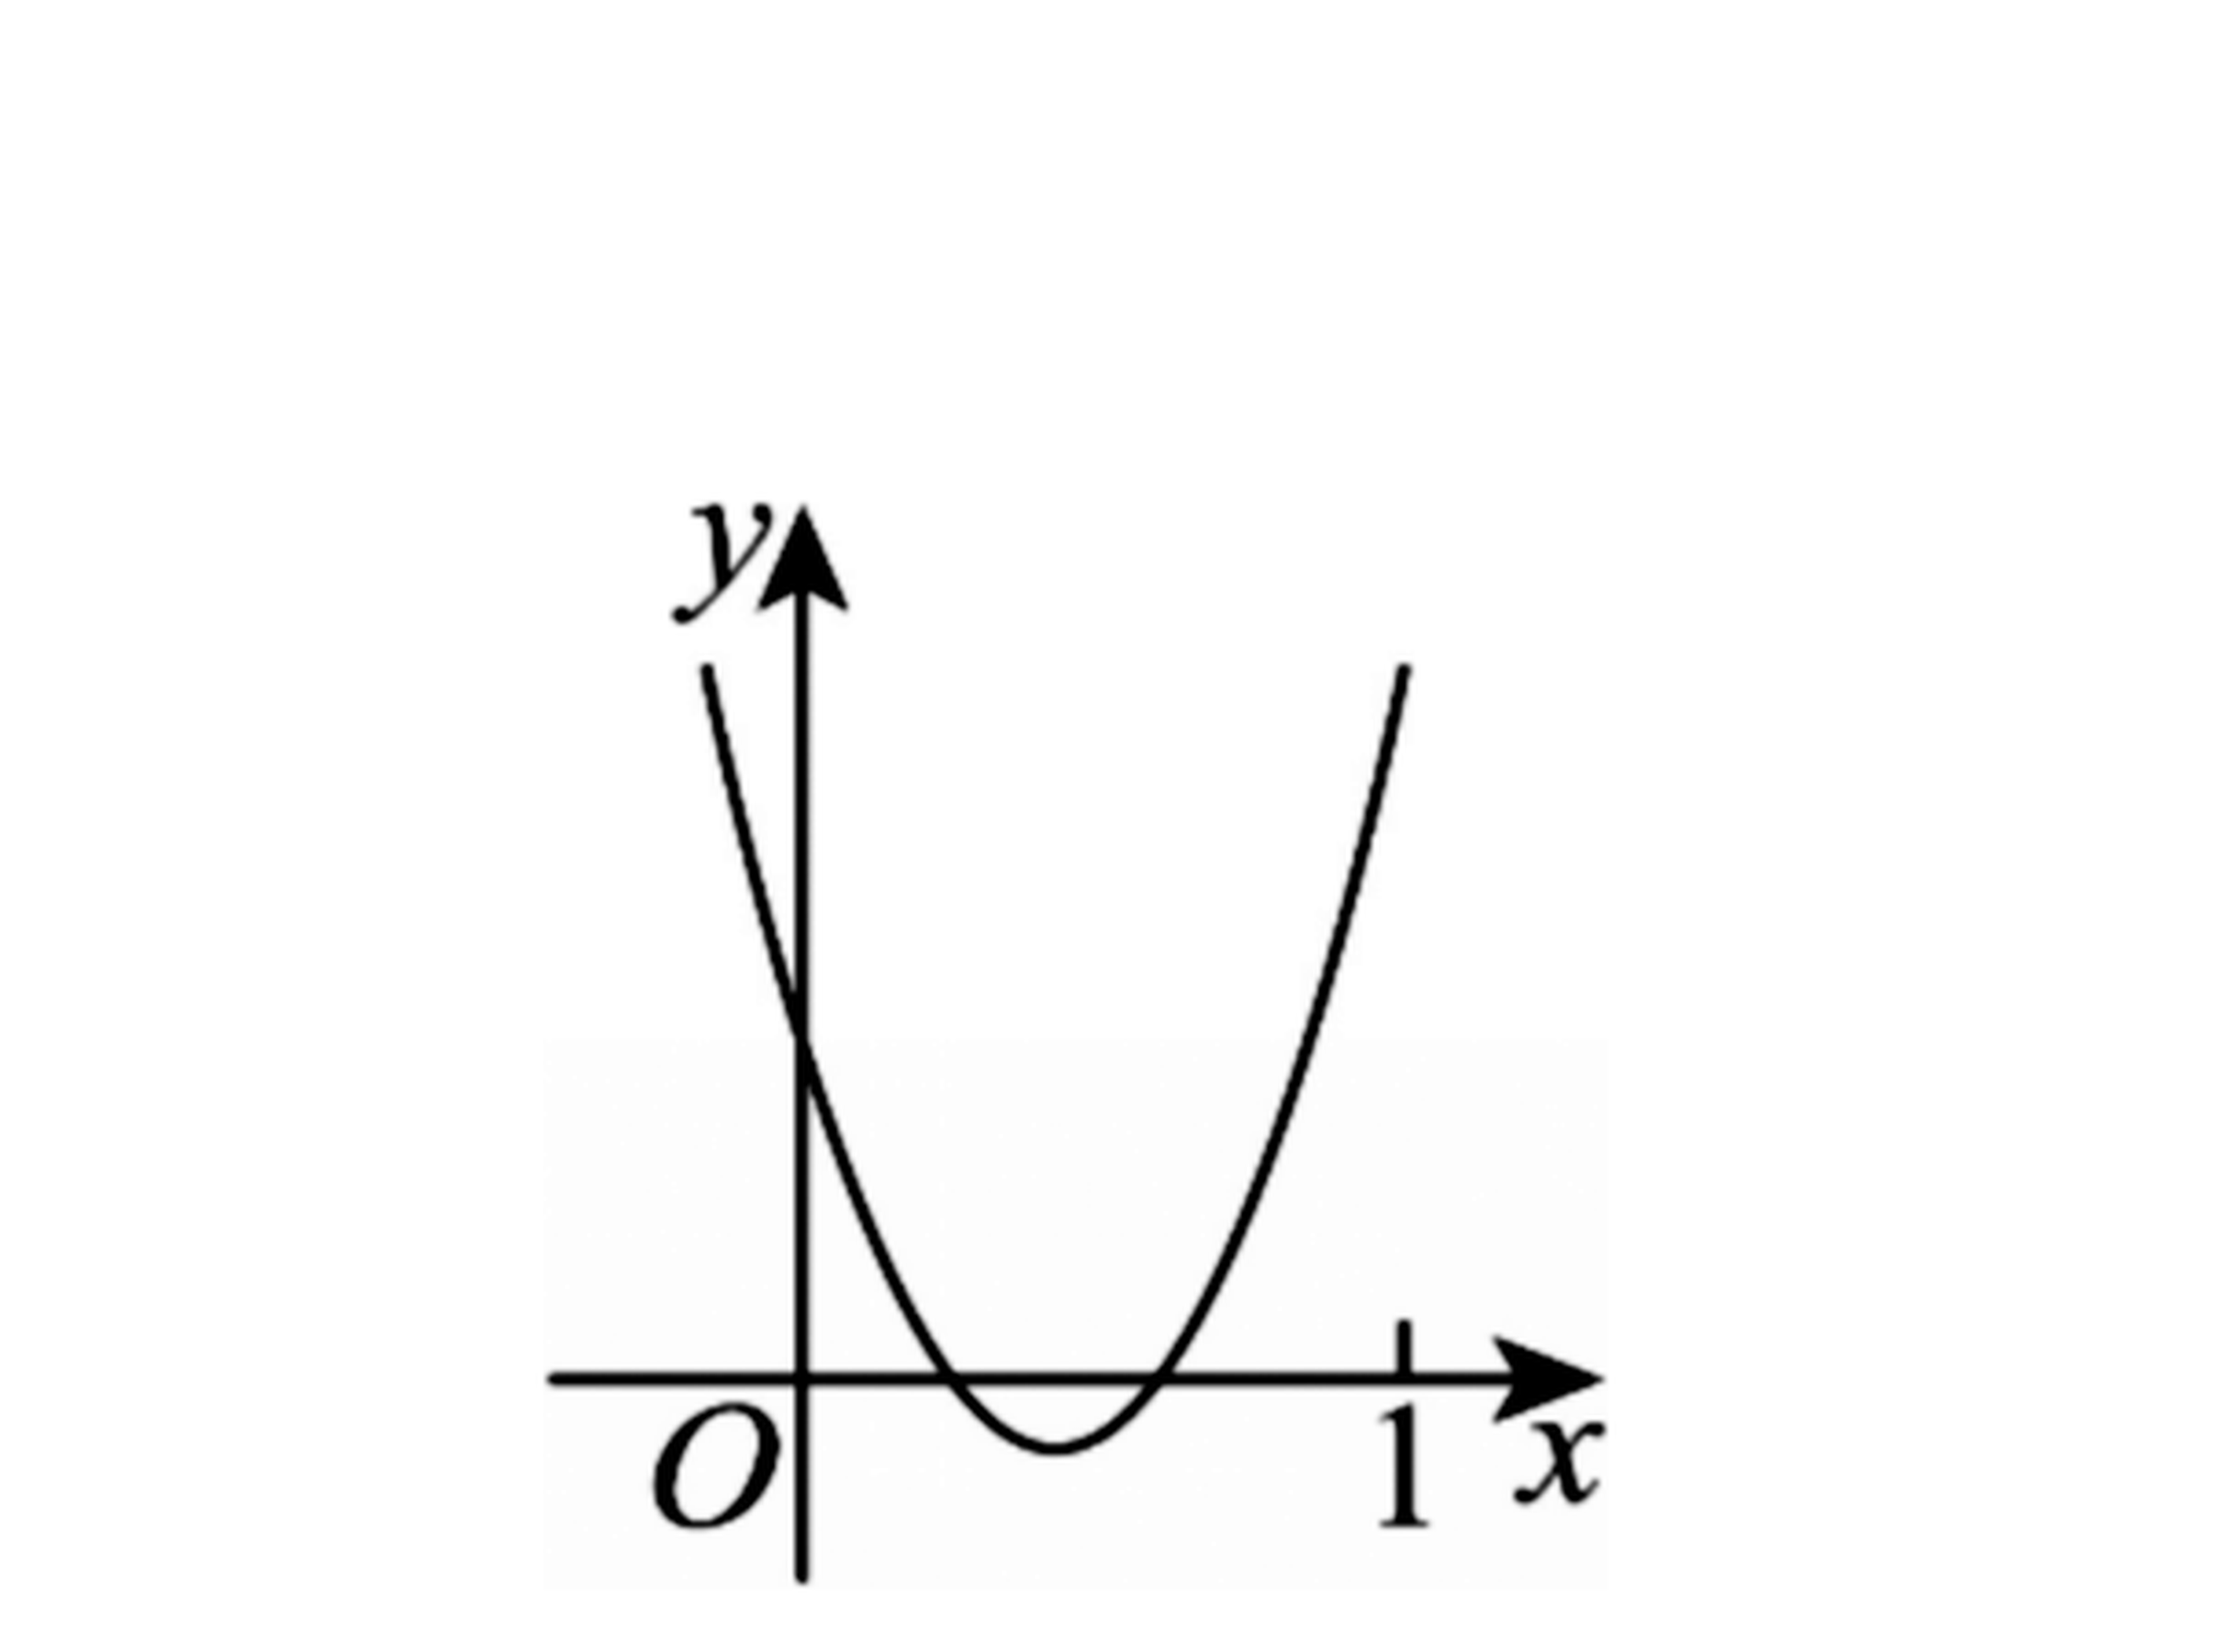
\includegraphics[width=0.32\textwidth]{figures/gao154_q15_stem.png}
\end{center}

\keepwithprev
\begin{center}
% 四幅指数函数图像选项取 05 页上半，按原卷 2×2 排布合并为一张，去粉色水印、去色、4× LANCZOS 放大；三版都出
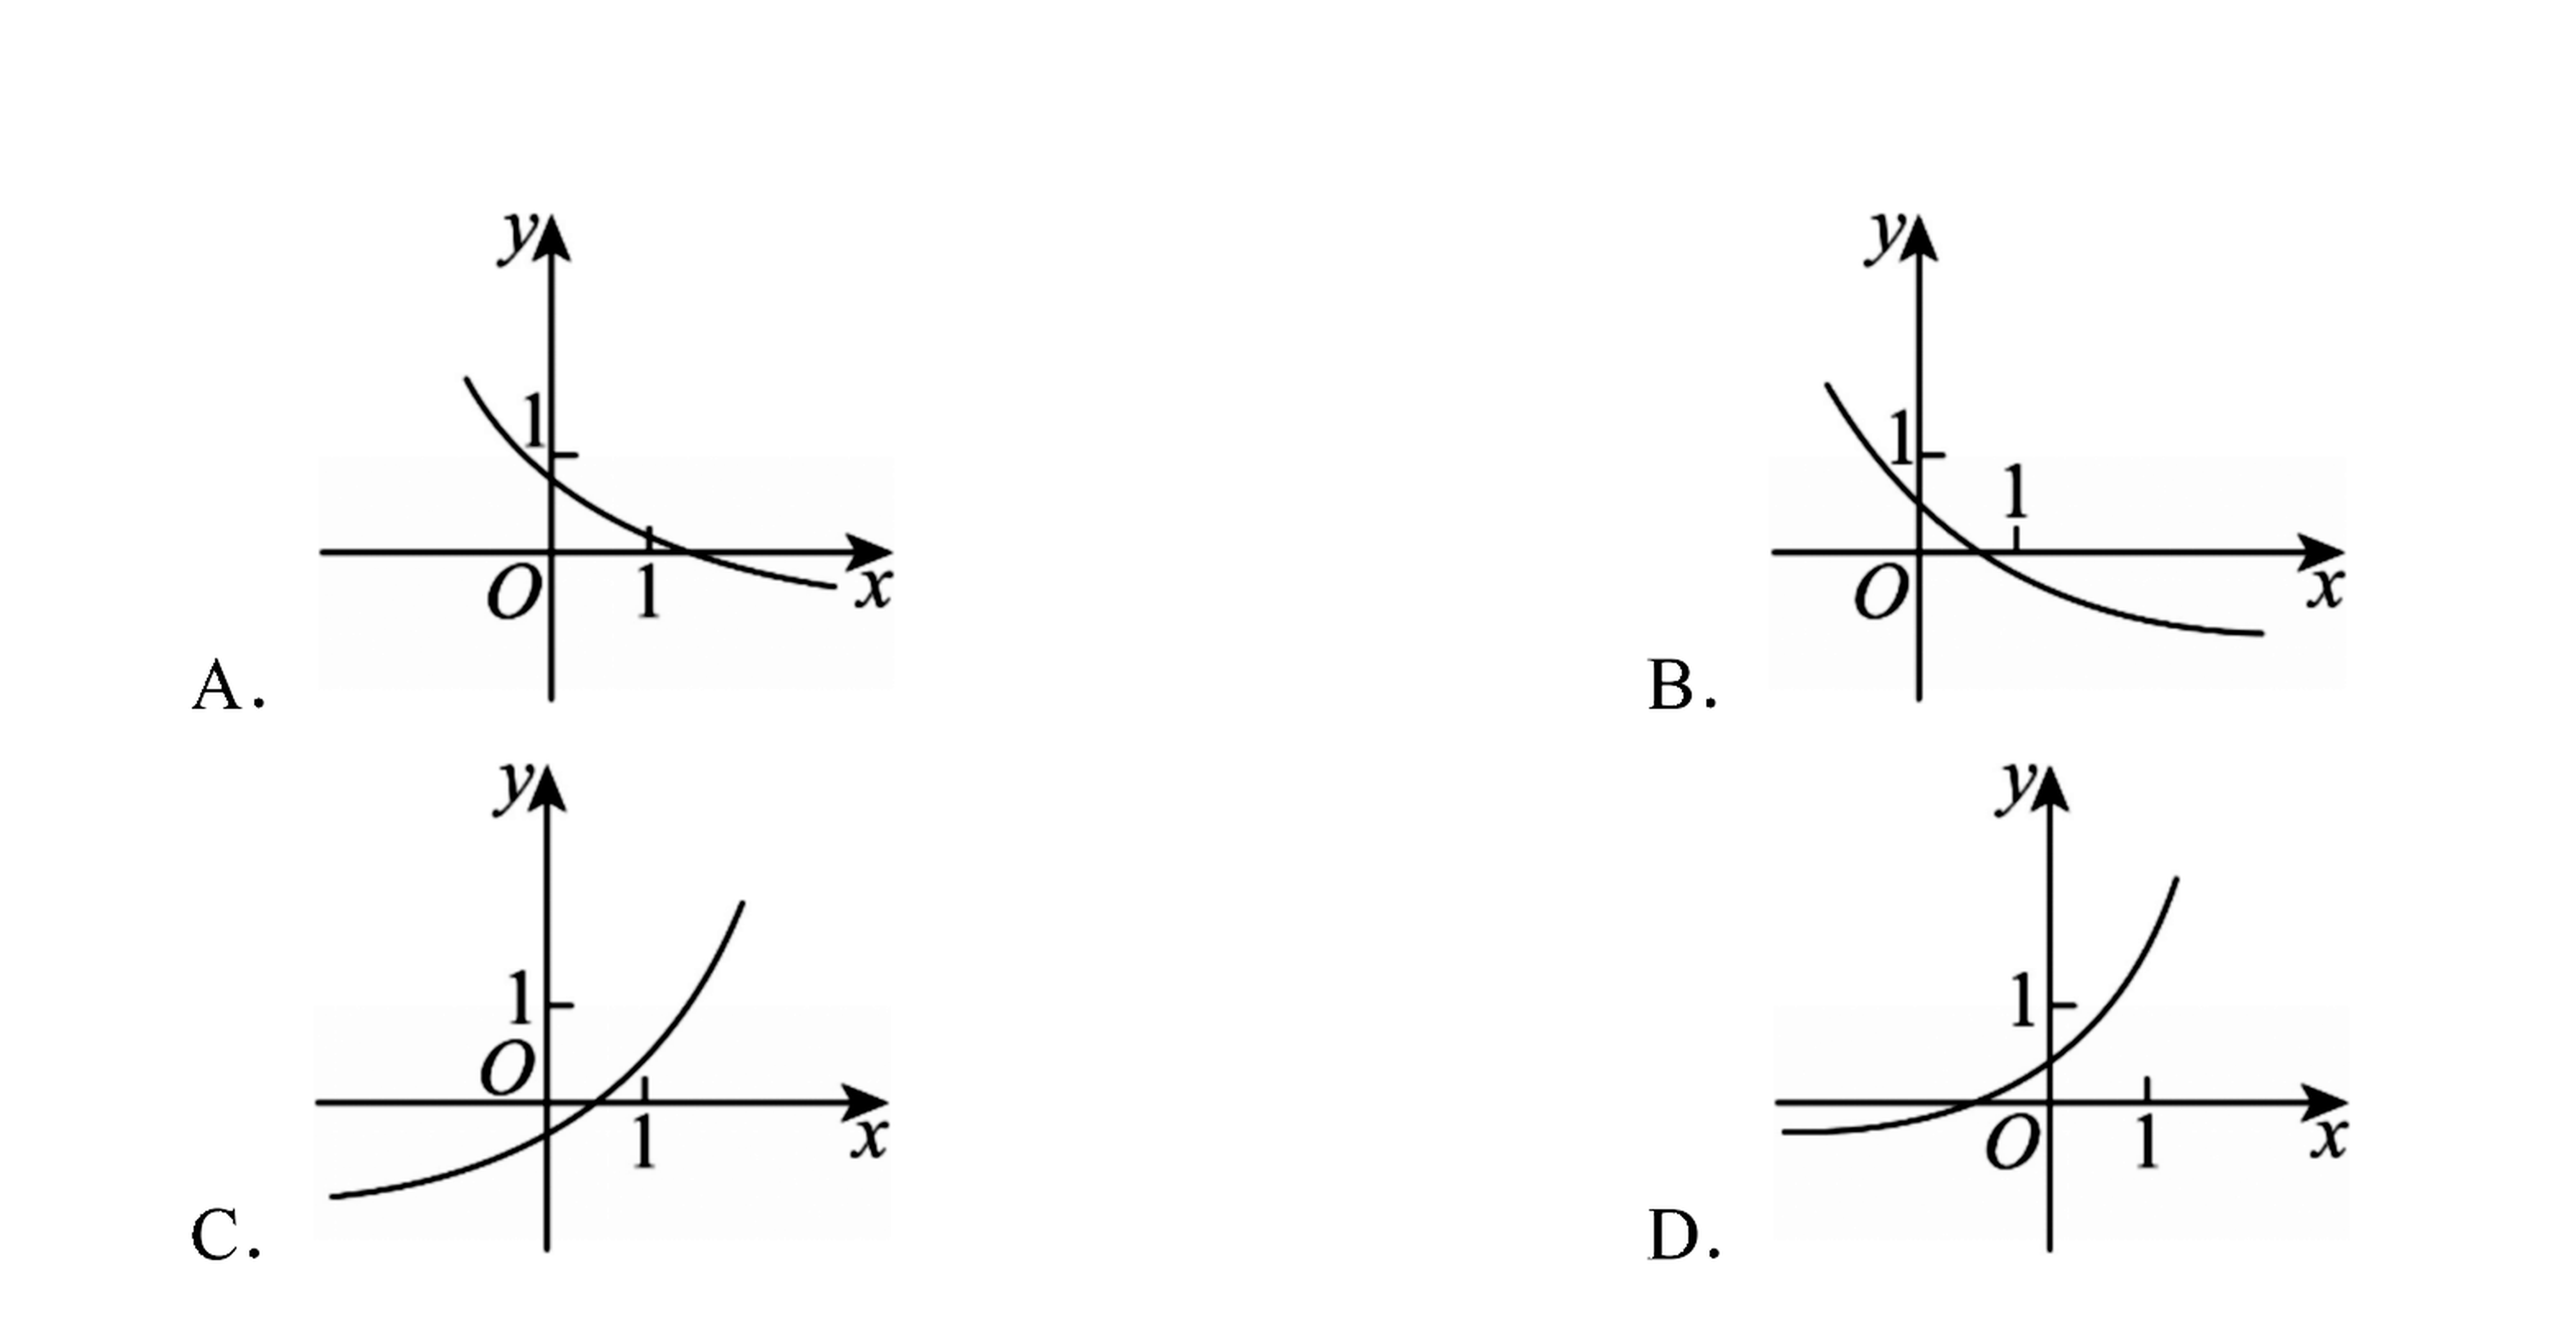
\includegraphics[width=0.80\textwidth]{figures/gao154_q15_opts.png}
\end{center}

\ifanswer
\solbegin
\step{由题意得 $0<a<b<1$，所以 $g(x)=a^x-b$ 在定义域 $\R$ 上严格减.}
\step{$g(0)=a^0-b=1-b>0$，$g(1)=a^1-b=a-b<0$，故 B 符合题意.}
\step{故选 $B$.}
\solend
\fi

% === Q16 === 高斯取整；解析 13 行，故选 C
\item 设 $[a]$ 表示不超过 $a$ 的最大整数，如 $[1.2]=1$，$[-3.2]=-4$，若 $x$、$y$、$z$ 为正实数，则 $\left[\dfrac{y+z}{x}\right]+\left[\dfrac{z+x}{y}\right]+\left[\dfrac{x+y}{z}\right]$ 的最小值为\mbox{（\quad）}

\keepwithprev
A. 2\qquad\qquad B. 3\qquad\qquad C. 4\qquad\qquad D. 6

\ifanswer
\solbegin
\step{若 $x$、$y$、$z$ 为正实数，}
\step{结合基本不等式得 $\dfrac{y+z}{x}+\dfrac{z+x}{y}+\dfrac{x+y}{z}=\dfrac yx+\dfrac xy+\dfrac zx+\dfrac xz+\dfrac zy+\dfrac yz$}
\step{$\geqslant2\sqrt{\dfrac yx\cdot\dfrac xy}+2\sqrt{\dfrac zx\cdot\dfrac xz}+2\sqrt{\dfrac zy\cdot\dfrac yz}=6$，当且仅当 $x=y=z$ 时取等号，}
\step{即 $\dfrac{y+z}{x}$，$\dfrac{z+x}{y}$，$\dfrac{x+y}{z}$ 中至少有一个不小于 2，不妨设 $\dfrac{y+z}{x}\geqslant\dfrac{z+x}{y}\geqslant\dfrac{x+y}{z}$，}
\step{$[a]$ 表示不超过 $a$ 的最大整数和 $\dfrac{y+z}{x}$，$\dfrac{z+x}{y}$，$\dfrac{x+y}{z}$ 中至少有一个不小于 2，}% 原卷此行把两句连写，照录未改（见 ⑤ 3）
\step{得 $\left[\dfrac{y+z}{x}\right]\geqslant2$，所以 $\left[\dfrac{y+z}{x}\right]+\left[\dfrac{z+x}{y}\right]+\left[\dfrac{x+y}{z}\right]\geqslant2$，}
\step{假设 $\left[\dfrac{y+z}{x}\right]+\left[\dfrac{z+x}{y}\right]+\left[\dfrac{x+y}{z}\right]$ 的最小值为 2，$\left[\dfrac{y+z}{x}\right]=2$，$\left[\dfrac{z+x}{y}\right]+\left[\dfrac{x+y}{z}\right]=0$，}
\step{所以 $2\leqslant\dfrac{y+z}{x}<3$，$0<\dfrac{z+x}{y}<1$，$0<\dfrac{x+y}{z}<1$，所以 $2<\dfrac{y+z}{x}+\dfrac{z+x}{y}+\dfrac{x+y}{z}<5$，}
\step{与 $\dfrac{y+z}{x}+\dfrac{z+x}{y}+\dfrac{x+y}{z}\geqslant6$ 矛盾，假设不成立，A 错误；}
\step{假设 $\left[\dfrac{y+z}{x}\right]+\left[\dfrac{z+x}{y}\right]+\left[\dfrac{x+y}{z}\right]$ 的最小值为 3，}
\step{则 $\left[\dfrac{y+z}{x}\right]=2$，$\left[\dfrac{z+x}{y}\right]=1$，$\left[\dfrac{x+y}{z}\right]=0$ 或 $\left[\dfrac{y+z}{x}\right]=3$，$\left[\dfrac{z+x}{y}\right]=\left[\dfrac{x+y}{z}\right]=0$，}
\step{同理可得 $3<\dfrac{y+z}{x}+\dfrac{z+x}{y}+\dfrac{x+y}{z}<6$，显然不成立，B 错误；}
\step{假设 $\left[\dfrac{y+z}{x}\right]+\left[\dfrac{z+x}{y}\right]+\left[\dfrac{x+y}{z}\right]$ 的最小值为 4，易得 $4<\dfrac{y+z}{x}+\dfrac{z+x}{y}+\dfrac{x+y}{z}<7$，}
\step{若取 $x=100$，$y=103$，$z=104$，则 $\left[\dfrac{y+z}{x}\right]=2$，$\left[\dfrac{z+x}{y}\right]=1$，$\left[\dfrac{x+y}{z}\right]=1$，}
\step{即 $\left[\dfrac{y+z}{x}\right]+\left[\dfrac{z+x}{y}\right]+\left[\dfrac{x+y}{z}\right]=4$，假设成立，C 正确，D 错误.}
\step{故选 $C$.}
\solend
\fi

\end{enumerate}

\bigsec{三、解答题}

\begin{enumerate}
\setcounter{enumi}{16}

% === Q17 === $B\subset A$ 单线照录；cases 块；解析 5 行
\item 设集合 $A=\{x\mid x^2+2x-3<0\}$，集合 $B=\{x\mid\lvert x+a\rvert<1\}$.

(1) 若 $a=3$，求 $A\cup B$；

(2) 设命题 $p:x\in A$，命题 $q:x\in B$，若 $p$ 是 $q$ 成立的必要不充分条件，求实数 $a$ 的取值范围.

\ifanswer
\solbegin
\step{(1) $A=(-3,1)$，}
\step{当 $a=3$ 时，$\lvert x+3\rvert<1$，解得 $-4<x<-2$，所以 $B=(-4,-2)$，}
\step{所以 $A\cup B=(-4,1)$.}
\step{(2) 因为 $p$ 是 $q$ 成立的必要不充分条件，所以 $B\subset A$.}
\step{因为 $A=(-3,1)$，$B=(-a-1,-a+1)$，所以 $\begin{cases}-a-1\geqslant-3\\-a+1<1\end{cases}$ 或 $\begin{cases}-a-1>-3\\-a+1\leqslant1\end{cases}$，解得 $0\leqslant a\leqslant2$.}
\solend
\fi

% === Q18 === 判别式 \Delta 两处照录；解析 9 行
\item 已知关于 $x$ 的一元二次方程 $x^2-mx+4m^2-3=0$ 的两个实根分别为 $x_1,x_2$.

(1) 若 $x_1,x_2$ 满足 $x_1+x_2=x_1x_2$，求实数 $m$ 的值；

(2) 求 $x_1^2+x_2^2$ 的最小值.

\ifanswer
\solbegin
\step{(1) 由韦达定理 $x_1+x_2=m$，$x_1x_2=4m^2-3$，}
\step{$\Delta=m^2-4(4m^2-3)=-15m^2+12\geqslant0$，即 $m^2\leqslant\dfrac45$.}
\step{由 $x_1+x_2=x_1x_2$ 得 $m=4m^2-3$，即 $4m^2-m-3=0$，}
\step{解得 $m=1$ 或 $m=-\dfrac34$.}
\step{$m=1$ 时 $m^2=1>\dfrac45$，$\Delta<0$，舍去；}
\step{$m=-\dfrac34$ 时 $m^2=\dfrac9{16}<\dfrac45$，符合，故 $m=-\dfrac34$.}
\step{(2) $x_1^2+x_2^2=(x_1+x_2)^2-2x_1x_2=m^2-2(4m^2-3)=-7m^2+6$，}
\step{函数 $y=-7m^2+6$ 开口向下，对称轴为 $m=0$，}% 原卷此处称求「最小值」，实为闭区间 $m^2\le\frac45$ 上的最小值，照录未改（见 ⑤ 4）
\step{故 $y_{\min}=-7\cdot\dfrac45+6=-\dfrac{28}{5}+\dfrac{30}{5}=\dfrac25$.}
\solend
\fi

% === Q19 === 全称命题；cases 块；解析 9 行
\item 设命题 $p$：对任意 $x\in\R$，不等式 $2mx^2+2mx+1>0$ 恒成立，$q:m\in\{m\mid\log_2(m-1)<1\}$.

(1) 若 $p$ 为真命题，求实数 $m$ 的取值范围；

(2) 若命题 $p$、$q$ 有且只有一个是真命题，求实数 $m$ 的取值范围.

\ifanswer
\solbegin
\step{(1) 由 $p$ 为真命题，得 $\forall x\in\R$，不等式 $2mx^2+2mx+1>0$ 恒成立，}
\step{当 $m=0$ 时，$1>0$ 恒成立；}
\step{当 $m\ne0$ 时，$\begin{cases}2m>0\\\Delta=4m^2-8m<0\end{cases}$，解得 $0<m<2$；}
\step{综上，$0\leqslant m<2$，即 $m$ 的取值范围是 $[0,2)$；}
\step{(2) 若 $q$ 为真，则有 $\log_2(m-1)<1$，得 $0<m-1<2$，解得 $1<m<3$，}
\step{因此命题 $q:m\in\{m\mid1<m<3\}$，由 (1) 得命题 $p:\{m\mid0\leqslant m<2\}$，}
\step{而命题 $p$、$q$ 有且只有一个是真命题，}
\step{当 $p$ 真 $q$ 假时，$\begin{cases}0\leqslant m<2\\m\leqslant1\text{ 或 }m\geqslant3\end{cases}$，解得 $0\leqslant m\leqslant1$，}
\step{当 $p$ 假 $q$ 真时，$\begin{cases}m<0\text{ 或 }m\geqslant2\\1<m<3\end{cases}$，解得 $2\leqslant m<3$，}
\step{故实数 $m$ 的取值范围是 $\{m\mid0\leqslant m\leqslant1\text{ 或 }2\leqslant m<3\}$.}
\solend
\fi

% === Q20 === Labubu 成本题；解析 10 行
\item Labubu 公司拟在 2027 年初推出智能机器人系列玩偶（单位：套）. 根据以往经验，其中一条生产线每月生产 $x$ 套玩具的成本 $P$ 由两部分费用（单位：元）构成：

(i) 固定成本（与生产玩具套数 $x$ 无关），总计 160000 元；

(ii) 每生产 $x$ 套需另投入的生产成本 $c(x)$ 元，其中 $c(x)=10x+\dfrac1{100}x^2$.

(1) 假设该生产线每月生产出的玩具能全部售出，问：该生产线每月生产玩具多少套时，可使得平均每套所需成本费用最少？此时每套玩具的成本费用是多少？

(2) 假设该生产线每月生产出的玩具能全部售出，但随着 $x$ 的增大，每月生产所需的直接总成本在急剧增加，因此售价也需随着 $x$ 的增大而适当增加. 设每套玩具的售价为 $q(x)$ 元，$q(x)=a+\dfrac xb$（$a,b\in\R$）. 若当月产量为 10000 套时利润最大，此时每套售价为 150 元，试求 $a,b$ 的值.（利润=销售收入$-$成本费用）

\ifanswer
\solbegin
\step{(1) 每月总成本 $P=160000+10x+\dfrac1{100}x^2$，}
\step{平均每套成本为 $\dfrac Px=\dfrac{160000}{x}+10+\dfrac x{100}\geqslant10+2\sqrt{\dfrac{160000}{x}\cdot\dfrac x{100}}=90$.}
\step{等号成立当且仅当 $\dfrac{160000}{x}=\dfrac x{100}$ 时，即 $x=4000$ 时取等号，}
\step{所以每月生产 4000 套时平均每套成本最少，此时每套成本为 90 元.}
\step{(2) 利润 $W(x)=x\cdot q(x)-P=\left(\dfrac1b-\dfrac1{100}\right)x^2+(a-10)x-160000$.}
\step{要在 $x=10000$ 处取得最大值，需 $\dfrac1b-\dfrac1{100}<0$，且对称轴为 $x=10000$，}
\step{故 $-\dfrac{a-10}{2\left(\frac1b-\frac1{100}\right)}=10000$，即 $a-10=-20000\left(\dfrac1b-\dfrac1{100}\right)$.}
\step{又 $q(10000)=a+\dfrac{10000}{b}=150$.}
\step{令 $t=\dfrac1b$，则 $a=150-10000t$，}
\step{代入上式 $140-10000t=-20000t+200$，解得 $t=\dfrac3{500}$，即 $b=\dfrac{500}{3}$；}
\step{再由 $a=150-10000\times\dfrac3{500}=150-60=90$，所以 $a=90$，$b=\dfrac{500}{3}$.}
\solend
\fi

% === Q21 === $A^+$／$A^-$ 新定义；$A\subseteq$ 带下划线照录、\varnothing；解析 16 行
\item 设集合 $A$ 为非空数集，定义 $A^+=\{x\mid x=a+b,a,b\in A\}$，$A^-=\{x\mid x=\lvert a-b\rvert,a,b\in A\}$.

(1) 若集合 $A=\{-1,1\}$，写出集合 $A^+$ 及 $A^-$；

(2) 若集合 $A=\{x_1,x_2,x_3,x_4\}$，$x_1<x_2<x_3<x_4$，且 $A^-=A$，求证：$x_1+x_4=x_2+x_3$；

(3) 若集合 $A\subseteq\{x\mid0\leqslant x\leqslant2020,x\in\N\}$，且 $A^+\cap A^-=\varnothing$，求集合 $A$ 元素的个数的最大值.

\ifanswer
\solbegin
\step{(1) 由 $A=\{-1,1\}$，得 $A^+=\{-2,0,2\}$，$A^-=\{0,2\}$；}
\step{(2) 由于集合 $A=\{x_1,x_2,x_3,x_4\}$，$x_1<x_2<x_3<x_4$，且 $A^-=A$，}
\step{所以 $A^-$ 中也只包含四个元素，即 $A^-=\{0,x_2-x_1,x_3-x_1,x_4-x_1\}$，}
\step{剩下的 $x_3-x_2=x_4-x_3=x_2-x_1$，所以 $x_1+x_4=x_2+x_3$；}
\step{(3) 设 $A=\{a_1,a_2,\cdots,a_k\}$ 满足题意，其中 $a_1<a_2<\cdots<a_k$，}
\step{则 $2a_1<a_1+a_2<a_1+a_3<\cdots<a_1+a_k<a_2+a_k<a_3+a_k<\cdots<a_{k-1}+a_k<2a_k$，所以 $\lvert A^+\rvert\geqslant2k-1$，}
\step{且 $a_1-a_1<a_2-a_1<a_3-a_1<\cdots<a_k-a_1$，所以 $\lvert A^-\rvert\geqslant k$，}
\step{因为 $A^+\cap A^-=\varnothing$，所以 $\lvert A^+\cup A^-\rvert=\lvert A^+\rvert+\lvert A^-\rvert\geqslant3k-1$，}
\step{$A^+\cup A^-$ 中最小的元素为 0，最大的元素为 $2a_k$，所以 $\lvert A^+\cup A^-\rvert\leqslant2a_k+1$，}
\step{所以 $3k-1\leqslant2a_k+1\leqslant4041$（$k\in\N^*$），所以 $k\leqslant1347$，}
\step{实际上当 $A=\{674,675,676,\cdots,2020\}$ 时满足题意，证明如下：}
\step{设 $A=\{m,m+1,m+2,\cdots,2020\}$，$m\in\N$，}
\step{则 $A^+=\{2m,2m+1,2m+2,\cdots,4040\}$，$A^-=\{0,1,2,\cdots,2020-m\}$，}
\step{由题意得 $2020-m<2m$，即 $m>673\dfrac13$，}
\step{故 $m$ 的最小值为 674，于是当 $m=674$ 时，$A$ 中元素最多，}
\step{即 $A=\{674,675,676,\cdots,2020\}$ 时满足题意，}
\step{综上所述，集合 $A$ 中元素的个数的最大值是 1347.}
\solend
\fi

\end{enumerate}

\bigsec{附加题}

\begin{enumerate}

% === 附加题 1 === 另起编号 1；「n 元集和集」弯引号；解析 6 行
\item 设集合 $A=\{a_1,a_2,a_3,a_4\}$，$C=\{2,3,4,6\}$，新定义：集合 $A$ 中所有含 $n$ 个元素的子集中 $n$ 个元素之和的不同值组成的集合为“$n$ 元集和集”. 若 $A$ 的“3 元集和集”为 $C$，则集合 $A=$\blankline[4.4em].

\ifanswer
\solbegin
\step{集合 $A$ 的 3 元子集共有 4 个：$\{a_1,a_2,a_3\}$，$\{a_1,a_2,a_4\}$，$\{a_1,a_3,a_4\}$，$\{a_2,a_3,a_4\}$，}
\step{集合 $C=\{a_1+a_2+a_3,a_1+a_2+a_4,a_1+a_3+a_4,a_2+a_3+a_4\}$，}
\step{不妨令 $a_1<a_2<a_3<a_4$，}
\step{则 $a_1+a_2+a_3<a_1+a_2+a_4<a_1+a_3+a_4<a_2+a_3+a_4$，}
\step{而 $C=\{2,3,4,6\}$，因此 $\begin{cases}a_1+a_2+a_3=2\\a_1+a_2+a_4=3\\a_1+a_3+a_4=4\\a_2+a_3+a_4=6\end{cases}$，相加化简得 $a_1+a_2+a_3+a_4=5$，}
\step{解得 $a_1=-1$，$a_2=1$，$a_3=2$，$a_4=3$，所以 $A=\{-1,1,2,3\}$.}
\solend
\fi

% === 附加题 2 === 解析配图（仅答案版出）；四选项；解析 15 行，故选 A
\item 已知函数 $f(x)=\log_p x+q$，其中 $p>0$ 且 $p\ne1$，曲线 $y=f(x)$ 经过 $P(1,2)$、$Q(2,3)$ 两点. 设 $g(x)=f(x)\cdot[f(x)-2]$，若 $\lvert g(a)\rvert=\lvert g(b)\rvert=\lvert g(c)\rvert=\lvert g(d)\rvert$，且 $a<b<c<d$，则 $ad(b+c)$ 的取值范围为\mbox{（\quad）}

\keepwithprev
A. $\left(\dfrac14,\dfrac5{16}\right)$\qquad B. $\left(\dfrac18,\dfrac5{16}\right)$\qquad C. $\left(\dfrac14,\dfrac25\right)$\qquad D. $\left(\dfrac18,\dfrac25\right)$

\ifanswer
\solbegin
\step{函数 $f(x)=\log_p x+q$，且曲线 $y=f(x)$ 经过点 $P(1,2)$ 和 $Q(2,3)$，}
\step{所以 $\begin{cases}f(1)=q=2\\f(2)=\log_p2+q=3\end{cases}$，解得 $p=2$，$q=2$，$f(x)=\log_2 x+2$.}
\step{不妨设 $\lvert g(x)\rvert=k$，令 $\log_2 x=m$，则 $f(x)\cdot[f(x)-2]=m(m+2)=m^2+2m$，}
\step{画出函数 $y=\lvert m^2+2m\rvert$ 的图象，如图所示，}
\begin{center}
% $y=|m(m+2)|$ 图像取 11 页右上，去粉色水印、去色、4× LANCZOS 放大；仅答案版出
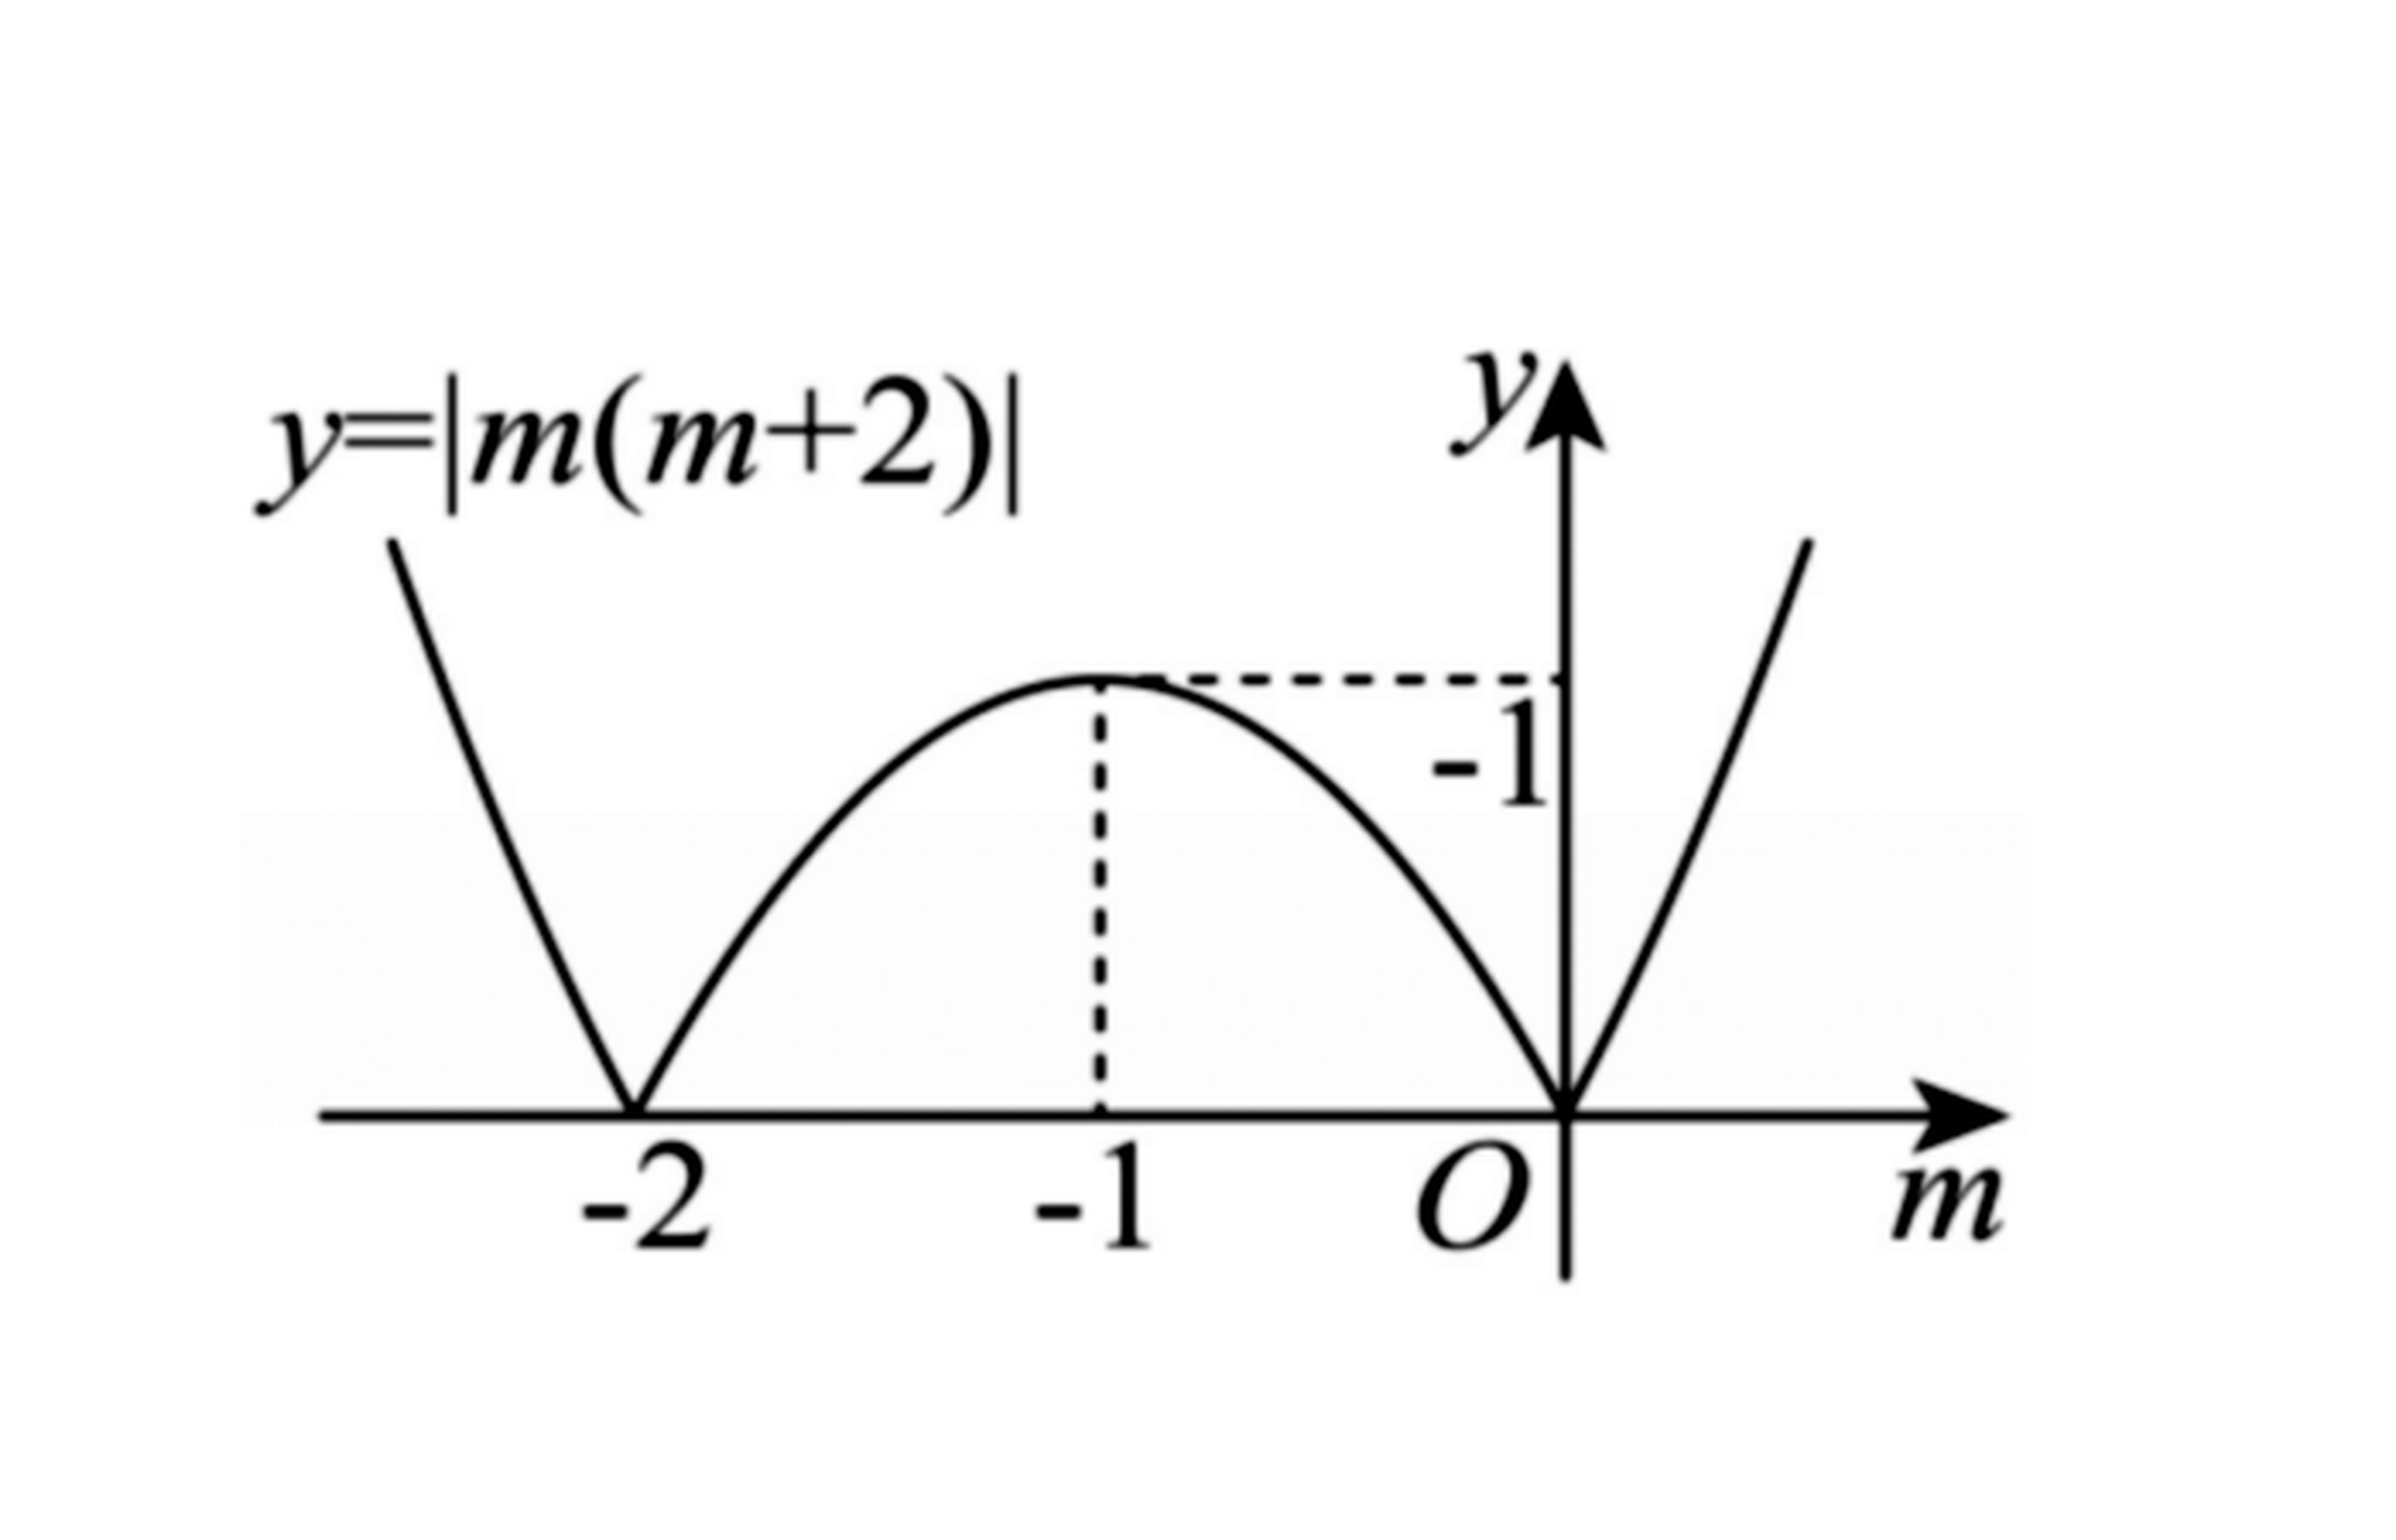
\includegraphics[width=0.46\textwidth]{figures/gao154_fujia2.png}
\end{center}
\step{由图像得 $k\in(0,1)$，}
\step{所以方程 $m^2+2m=k$ 和 $m^2+2m=-k$ 各有两个不同的根，}
\step{其中方程 $m^2+2m-k=0$ 的两根为 $m=-1\pm\sqrt{1+k}$，}
\step{方程 $m^2+2m+k=0$ 的两根为 $m=-1\pm\sqrt{1-k}$，}
\step{所以 $m_1=-1-\sqrt{1+k}$，$m_2=-1-\sqrt{1-k}$，$m_3=-1+\sqrt{1-k}$，$m_4=-1+\sqrt{1+k}$，且 $m_1<m_2<m_3<m_4$，}
\step{由 $m=\log_2 x$，则 $x=2^m$，}
\step{所以 $a=2^{-1-\sqrt{1+k}}$，$b=2^{-1-\sqrt{1-k}}$，$c=2^{-1+\sqrt{1-k}}$，$d=2^{-1+\sqrt{1+k}}$，}
\step{所以 $ad=2^{-1-\sqrt{1+k}}\times2^{-1+\sqrt{1+k}}=2^{(-1-\sqrt{1+k})+(-1+\sqrt{1+k})}=2^{-2}=\dfrac14$，}
\step{$b+c=2^{-1-\sqrt{1-k}}+2^{-1+\sqrt{1-k}}=\dfrac{2^{-\sqrt{1-k}}+2^{\sqrt{1-k}}}{2}$，}
\step{令 $s=\sqrt{1-k}$，其中 $s\in(0,1)$，则 $b+c=\dfrac12\left(2^{-s}+2^s\right)$，}
\step{设函数 $y=2^s+\dfrac1{2^s}$，令 $r=2^s\in(1,2)$，所以 $y=r+\dfrac1r$ 在 $(1,2)$ 上严格增，}
\step{所以函数 $y=2^s+\dfrac1{2^s}$ 在 $(0,1)$ 上严格增，所以 $y=2^s+\dfrac1{2^s}\in\left(2,\dfrac52\right)$，}
\step{所以 $b+c=\dfrac{2^{-s}+2^s}{2}\in\left(1,\dfrac54\right)$，$ad(b+c)=\dfrac{b+c}{4}\in\left(\dfrac14,\dfrac5{16}\right)$，}
\step{所以 $ad(b+c)$ 的取值范围是 $\left(\dfrac14,\dfrac5{16}\right)$，故选 $A$.}
\solend
\fi

\end{enumerate}

\end{document}
"
% 紧凑版：xelatex "\def\iscompact{1}% 高一154_徐汇中学_期中.tex
%   —— 高一上数学"2026-2027 年徐汇中学高一上期中"（试卷版/答案版/紧凑版）
% 试卷版：xelatex 高一154_徐汇中学_期中.tex
% 答案版：xelatex "\def\isanswer{1}% 高一154_徐汇中学_期中.tex
%   —— 高一上数学"2026-2027 年徐汇中学高一上期中"（试卷版/答案版/紧凑版）
% 试卷版：xelatex 高一154_徐汇中学_期中.tex
% 答案版：xelatex "\def\isanswer{1}\input{高一154_徐汇中学_期中.tex}"
% 紧凑版：xelatex "\def\iscompact{1}\input{高一154_徐汇中学_期中.tex}"
%
% ① 原始材料：微信公众号"魔都数学加油站"文章，连载"27学年高一154"，原文标题
% "27学年高一154——2026-2027年上海市徐汇中学高一上期中"；
% 原文链接：https://mp.weixin.qq.com/s/Qs2T7Zwsug-KKFE2wefDUg 。
% 正文为 12 张 PNG 页（01/03/04/05/07/11/12 为 2560×3620，
% 02/06/08/09/10 为 4762×6735，同一篇各页分辨率混排，逐页按各自分辨率裁图核对）。
% 体例：讲评版——一、填空题 3—12（10 题）、二、选择题 13—16（4 题）、
% 三、解答题 17—21（5 题）、附加题 1—2（2 题，原卷**另起编号**"1." "2."，
% 不与正题连号，同 高一a 成例），共 21 题；全卷每题均印【解析】
% （逐题核实，见 ② ②）。题目、答案、解析均据原图转录；卷面粉红色水印
% "魔都数学加油站"及公众号页脚未录入。
% 全卷插图清单（逐页通读 12 页确认）：3 组——
%   · Q15 题干配图（$f(x)=(x-a)(x-b)$ 抛物线，04 页右下：x/y 轴、O、1、
%     开口向上两零点均在 (0,1) 内），三版都出，裁 figures/gao154_q15_stem.png；
%   · Q15 四幅图像选项（05 页上半 2×2 排布，A/B/C/D 四幅指数函数图像，
%     合并成一张，照 高一136 Q13/Q22 成例），三版都出，
%     裁 figures/gao154_q15_opts.png；
%   · 附加题第 2 题解析配图（$y=\lvert m(m+2)\rvert$ 图像，11 页右上：
%     W 形折线、$-2$、$-1$、O、虚线 $y=1$ 与 $m=-1$），仅答案版出，
%     裁 figures/gao154_fujia2.png；
%   3 图均取自原卷截图，去粉色水印、去色、4× LANCZOS 放大；Q15 题干图
%   左侧题干残字"的图"已裁白。其余各页逐页确认无其它题目配图、无表格；
%   12 页下半仅水印、无正文。
%
% 卷首标题：原卷印作"2026-2027 年徐汇中学高一上期中"，年份区间按全稿惯例排 en dash；
% 原卷卷面未印副标题，本稿按同期中卷知识模块口径补出"集合与常用逻辑用语、不等式、函数"。
%
% ② 与原卷的排版差异：
%   ① 原文从第 3 题起，本稿保留原题号；共 21 题四节，正题到 21，附加题另起编号
%      1—2（\bigsec{附加题} 后 \begin{enumerate} 不 \setcounter，同 高一a 成例）；
%   ② 全 21 题均印【解析】、用 \solbegin…\solend，无只印【答案】或答案印括号内的题；
%      四道正题选择题答案在解析末句"故选 C／A／B／C"（Q13—Q16）、附加题第 2 题
%      答案在解析末句"故选 A"，括号 \mbox{（\quad）} 留空、不另提 \ans{}；
%      答案版【答案】/【解析】标记数 = 21 = 全卷题数；
%   ③ 原卷卷面未印副标题，本稿按知识模块口径补出；
%   ④ 原卷填空横线按全稿惯例排 \blankline[4.4em]；选择题括号排 \mbox{（\quad）}、
%      四道正题选择题与附加题第 2 题的选项段前按惯例各加 \keepwithprev
%      （Q15 与附加题 2 的选项段是整块图，\keepwithprev 后接 \begin{center}）；
%      解答题不留作答区、不加 \anspace（原卷为讲评版）；
%   ⑤ 数集黑板粗体：Q4"$x,y\in R$"、Q9"$x\in\R$"、Q13 无、
%      Q15"定义域 $\R$"、Q19"$\forall x\in\R$"、Q21"$x\in\N$"与"$k\in\N^*$"、
%      Q20"$a,b\in\R$"、附加题 2 无——原卷印斜体或正体粗体 R/N/N*，
%      按全稿惯例归一 \R／\N／\N^*；绝对值排 \lvert…\rvert
%      （Q5、Q9、Q12、Q13、Q16、Q21、附加题 2），集合描述竖线排 \mid
%      （Q5、Q17、Q19、Q21），不等号按全稿惯例排 \leqslant／\geqslant；
%      空集 \varnothing（Q21 题干 (3)）；
%   ⑥ 子集符号逐处照录、不得统一：Q6 题干印"$\{1,2\}\subset M\subseteq\{1,2,3,4,5\}$"
%      （前单线 ⊂、后带下划线 ⊆，同句两形并用），解析亦两形并用；
%      Q17 解析 (2)"$B\subset A$"印单线 ⊂；Q21 题干 (3)"$A\subseteq\{x\mid\cdots\}$"
%      印带下划线 ⊆——逐处放大核，分别 \subset／\subseteq，照录未统一（见 ④）；
%   ⑦ 判别式 Δ/△：Q18 解析 (1)"$\Delta=m^2-4(4m^2-3)$"与 Q19 解析 (1)
%      "$\Delta=4m^2-8m<0$"两处均印等腰偏高粗三角、照录 \Delta；本卷无扁等边
%      细线 \triangle 用例（见 ④）；
%   ⑧ 中文弯引号照录：Q4"设 $x$、$y\in\R$. 若 $x+y>2$，则 $x>1$ 或 $y>1$"、
%      附加题 1"$n$ 元集和集"与"3 元集和集"；注释里一律 ASCII 引号；
%      数学式内 CJK 用 \text{}（Q5 解集描述"或"、Q19 集合描述的"或"）；
%   ⑨ "图像／图象"逐处放大核：Q15 题干与解析印"图象"（象，无亻）、
%      Q16 无、附加题 2 解析印"图象"与"图像"（"画出函数…的图象"、
%      "由图像得"——两形并用，逐处照录未统一）；Q13/Q14 无数集图像字样；
%      半角逗号在数学组之间是全稿惯例、非笔误，逐处照录（Q3、Q10、Q16、
%      Q18、Q20、Q21 的 $x_1,x_2$ 之类）；行末西文句点 ASCII `.`；
%      行中全角逗号／顿号照录（Q6"3，4，5"、Q20"（单位：元）"、
%      附加题 1"$a_1,a_2,a_3,a_4$"）；
%   ⑩ 复杂式照录别简化：Q3 $a^{\frac{12}{7}}\cdot\left(\frac17\right)^{\frac17}
%      \cdot\sqrt[7]{a^4}$ 与 $7^{-\frac17}a^{\frac{16}{7}}$、Q7 $x^{-m}$、
%      Q8 $\frac{b-2a+2}{2a}$、Q11 $\frac{9+4\sqrt2}{6}$、Q12 $506\frac29$ 与
%      $506\frac49$、Q16 高斯取整 $[a]$、Q20 $c(x)=10x+\frac1{100}x^2$ 与
%      $q(x)=a+\frac xb$、Q21 $A^+$／$A^-$ 与 $|A^+|\geqslant2k-1$、
%      附加题 2 $m=-1\pm\sqrt{1+k}$ 与 $ad(b+c)$；
%      \left…\right 不得拆到不同 $…$ 组（Q5 $\left\{x\mid\cdots\right\}$、
%      Q20 $\left(\frac1b-\frac1{100}\right)$、附加题 2 $\left(\frac14,\frac5{16}\right)$）；
%      cases 块一律 \begin{cases}…\end{cases}；
%   ⑪ 一条 \step = 原卷解析的一个印刷行，cases 块整体算一个印刷行；别并折行、
%      别拆行。Q11 九行、Q12 六行、Q16 十六行、Q20 十一行、Q21 十七行、
%      附加题 2 十八行均按印刷行逐条断，不丢行；
%   ⑫ 配图：Q15 题干小图（三版都出）放 \item 内题干之后 \begin{center}，
%      Q15 四幅选项图（三版都出）放 \keepwithprev 之后的 \begin{center}，
%      Q15 用 \needvspace 守卫把"题干＋两图"整块推走（守卫放 \item 之前，
%      见 高一145 Q14/Q20 与 高一136 Q13 成例）；附加题 2 解析配图（仅答案版出）
%      放 \ifanswer 内 \solbegin…\solend 的 \step 之间（高一73 第 16 题成例）；
%   ⑬ 原卷解析内无红色"法一／法二"之类小标题，故本卷无 \stepm；红色水印
%      "魔都数学加油站"不录入；
%   ⑭ 跨页续印按题合并：见 ⑥；
%
% ③ 行数复核：一条 \step = 原卷解析的一个印刷行，cases 块作一个印刷行计。
%   逐题数（主会话逐页核对定稿）：Q3：1；Q4：1；Q5：3；Q6：4；Q7：3；
%   Q8：1；Q9：5；Q10：4；Q11：9；Q12：6；Q13：5；Q14：4；Q15：3；
%   Q16：16；Q17：5；Q18：9；Q19：10；Q20：11；Q21：17；
%   附加题 1：6；附加题 2：18。
%   合计 141 条 \step（本卷无 \stepm），与原卷逐题印刷行相等。全卷 21 题
%   均设 \solbegin…\solend，答案版【答案】/【解析】标记数 = 21 = 全卷题数。
%
% ④ 判别式／子集符号结论（逐处放大原图照录、不得统一，主会话像素级复核）：
%   判别式：Q18 解析 (1)"$\Delta=m^2-4(4m^2-3)=-15m^2+12\geqslant0$"、
%      Q19 解析 (1)"$\Delta=4m^2-8m<0$"共 2 处，逐处放大确认印等腰偏高
%      粗三角（高>宽、右斜边粗），照录 \Delta；本卷无扁等边细线 \triangle
%      用例，无几何三角形符号。
%   子集：Q6 题干"$\{1,2\}\subset M\subseteq\{1,2,3,4,5\}$"前 ⊂ 单线、
%      后 ⊆ 带下划线（/tmp/gao154/z/zoom/q6_subset.png），解析两处同样两形
%      并用，分别照录 \subset／\subseteq；Q17 解析 (2)"$B\subset A$"单线
%      照录 \subset；Q21 题干 (3)"$A\subseteq\{x\mid\cdots\}$"带下划线
%      照录 \subseteq。本卷 ⊂ 与 ⊆ 混用逐处照录、不得统一。
%      空集 \varnothing（Q21 题干 (3)）、数集 \R／\N／\N^* 归一见 ② ⑤。
%
% ⑤ 存疑照录（放大原图确认，照录未改、正文对应处另有 % 注）：
%   1. Q7 题干印 $f(x)=(3m-1)x^{-m}$，解析首句却写"幂函数 $f(x)=x^\alpha$
%      的系数必须为 1"（用 $\alpha$ 作指数记号），随后 $f(2)=2^\alpha=8$
%      得 $\alpha=3$、$f(x)=x^3$——题干指数 $-m$ 与解析 $\alpha$ 记法不同，
%      系原卷记号前后不一，逐处照录未统一（放大 01/02 页确认）。
%   2. Q11 解析"因为 $u>0,v>0$，由基本不等式得 $\frac{4v}{u}+\frac{2u}{v}
%      \geqslant2\sqrt{\frac{4v}{u}\cdot\frac{2u}{v}}=4\sqrt2$"与
%      "所以 $\frac4u+\frac1v=\frac16\left(\frac4u+\frac1v\right)(2u+v)$"
%      照录，未把 $u,v$ 化简回 $x,y$。
%   3. Q16 解析把"$[a]$ 表示不超过 $a$ 的最大整数"与"和至少有一个不小于 2"
%      连写在同一行（原卷如此），照录未改；末行"假设成立，C 正确，D 错误"照录。
%   4. Q18 解析 (2)"函数 $y=-7m^2+6$ 开口向下，对称轴为 $m=0$"却称求
%      "$y_{\min}$"（实为在 $m^2\leqslant\frac45$ 闭区间上的最小值），
%      照录未改。
%   5. Q20 题干"$q(x)=a+\frac xb$（$a,b\in\R$）"与解析
%      "$W(x)=\left(\frac1b-\frac1{100}\right)x^2+(a-10)x-160000$"照录；
%      末行解得 $a=90,b=\frac{500}{3}$ 照录未化简。
%   6. Q21 题干 (3)"$A\subseteq\{x\mid0\leqslant x\leqslant2020,x\in\N\}$"
%      与解析"$3k-1\leqslant2a_k+1\leqslant4041$（$k\in\N^*$）"照录；
%      末行"集合 $A$ 中元素的个数的最大值是 1347"照录。
%   7. 附加题 1 解析"相加化简得 $a_1+a_2+a_3+a_4=5$"照录；
%      附加题 2 解析"由图像得 $k\in(0,1)$"与"由图像得"／"的图象"两形
%      并用逐处照录（见 ② ⑨）；末行"$ad(b+c)$ 的取值范围是
%      $\left(\frac14,\frac5{16}\right)$，故选 A"照录。
%   全卷除此 7 类外未发现其它笔误／自相矛盾处；21 题均印【解析】、
%   无只印【答案】或答案印括号内的题（见 ② ②）。
%
% ⑥ 跨页续印按题合并说明（逐页核实定稿）：Q3—Q5 题干＋解析在 01 页
%   （Q5 解析末 2 行续 01 页下半）；Q6、Q7 题干＋解析在 01 页下半
%   （Q7 解析余 2 行续 02 页顶）；Q8、Q9 题干＋解析在 02 页上半
%   （Q9 解析余 3 行续 02 页下半）；Q10 题干＋解析在 02 页下半；
%   Q11 题干＋解析前 6 行在 03 页上半、余 3 行续 03 页下半；
%   Q12 题干＋解析前 5 行在 03 页下半、末行续 04 页顶；"二、选择题"
%   标题与 Q13 题干＋选项＋解析在 04 页上半；Q14 题干＋选项＋解析、
%   Q15 题干＋题干配图在 04 页下半；Q15 四幅选项图＋解析、
%   Q16 题干＋选项＋解析首行在 05 页上半，Q16 解析余 12 行在
%   05 页下半—06 页上半；"三、解答题"标题与 Q17 题干＋两问＋解析
%   在 06 页下半；Q18 题干＋两问＋解析在 07 页上半—下半；
%   Q19 题干＋两问＋解析首行在 07 页下半，解析余 8 行在 08 页上半；
%   Q20 题干在 08 页下半，解析 (1) 4 行＋(2) 首 4 行在 08 页下半—09 页上半，
%   (2) 余 2 行在 09 页下半；Q21 题干＋三问＋解析 (1)(2) 4 行在
%   09 页下半—10 页上半，解析 (3) 余 12 行在 10 页上半—下半；
%   "附加题"标题与附加题 1 题干＋解析首 3 行在 10 页下半，
%   余 3 行续 11 页上半；附加题 2 题干＋选项＋解析前 3 行在 11 页上半，
%   解析配图＋余 12 行在 11 页下半—12 页上半，末行
%   "所以 $ad(b+c)$ 的取值范围是 $\left(\frac14,\frac5{16}\right)$，故选 A"
%   为全卷收尾（12 页下半仅水印、无正文）。
%   本稿按题连排，不丢行、不并折行；全卷末题为附加题第 2 题。
%
\documentclass[a4paper,11pt]{article}
\usepackage{common}

\begin{document}

\examtitlest[3]{2026--2027 年徐汇中学高一上期中}{集合与常用逻辑用语、不等式、函数}

\bigsec{一、填空题}

\begin{enumerate}
\setcounter{enumi}{2}

% === Q3 === 分数指数幂照录；解析 1 行
\item 已知 $a>0$，化简 $a^{\frac{12}{7}}\cdot\left(\dfrac17\right)^{\frac17}\cdot\sqrt[7]{a^4}=$\blankline[4.4em].

\ifanswer
\solbegin
\step{$a^{\frac{12}{7}}\cdot\left(\dfrac17\right)^{\frac17}\cdot\sqrt[7]{a^4}=a^{\frac{12}{7}}\cdot(7^{-1})^{\frac17}\cdot a^{\frac47}=7^{-\frac17}a^{\frac{16}{7}}$.}
\solend
\fi

% === Q4 === 反证法；中文弯引号照录；解析 1 行
\item 用反证法证明命题：“设 $x$、$y\in\R$. 若 $x+y>2$，则 $x>1$ 或 $y>1$”时，假设的内容应该是\blankline[4.4em].

\ifanswer
\solbegin
\step{由反证法得，假设的内容应该是 $x\leqslant1$ 且 $y\leqslant1$.}
\solend
\fi

% === Q5 === 分式不等式；cases 块；解析 3 行
\item 不等式 $\dfrac{2x+3}{x-1}\geqslant1$ 的解集为\blankline[4.4em].

\ifanswer
\solbegin
\step{$\dfrac{2x+3}{x-1}\geqslant1$，即 $\dfrac{2x+3}{x-1}-1\geqslant0$，$\dfrac{x+4}{x-1}\geqslant0$，}
\step{等价于 $\begin{cases}(x+4)(x-1)\geqslant0\\x-1\ne0\end{cases}$，解得 $x>1$ 或 $x\leqslant-4$，}
\step{故解集为 $\{x\mid x>1\text{ 或 }x\leqslant-4\}$.}
\solend
\fi

% === Q6 === ⊂ 与 ⊆ 并用照录；解析 4 行
\item 满足条件 $\{1,2\}\subset M\subseteq\{1,2,3,4,5\}$ 的集合 $M$ 的个数为\blankline[4.4em].

\ifanswer
\solbegin
\step{因为 $\{1,2\}\subset M\subseteq\{1,2,3,4,5\}$，所以集合 $M$ 必含有元素 1，2，}
\step{且至少含有元素 3，4，5 中的一个，}
\step{则集合 $M$ 的个数与集合 $\{3,4,5\}$ 的非空子集的个数一样，}
\step{所以集合 $M$ 的个数为 $2^3-1=7$.}
\solend
\fi

% === Q7 === 题干 $x^{-m}$、解析用 $x^\alpha$ 记法，原卷记号差异照录（见 ⑤ 1）；解析 3 行
\item 已知幂函数 $f(x)=(3m-1)x^{-m}$，且 $f(2)=8$，则 $f(m)=$\blankline[4.4em].

\ifanswer
\solbegin
\step{幂函数 $f(x)=x^\alpha$ 的系数必须为 1，所以 $3m-1=1$，得 $m=\dfrac23$.}
\step{又 $f(2)=2^\alpha=8=2^3$，故 $\alpha=3$，即 $f(x)=x^3$，}
\step{所以 $f(m)=f\left(\dfrac23\right)=\left(\dfrac23\right)^3=\dfrac8{27}$.}
\solend
\fi

% === Q8 === 换底公式；解析 1 行
\item 已知 $a=\lg2$，$b=\lg3$，用含 $a,b$ 的代数式表示 $\log_4 75=$\blankline[4.4em].

\ifanswer
\solbegin
\step{$\log_4 75=\dfrac{\lg\left(3\times\frac{10^2}{2^2}\right)}{\lg2^2}=\dfrac{\lg3+2-2\lg2}{2\lg2}=\dfrac{b-2a+2}{2a}$.}
\solend
\fi

% === Q9 === 三角不等式取等；解析 5 行
\item 设 $x\in\R$，则方程 $\lvert x-2\rvert+\lvert3x+1\rvert=\lvert2x+3\rvert$ 的解集是\blankline[4.4em].

\ifanswer
\solbegin
\step{由 $\lvert x-2\rvert=\lvert2-x\rvert$，故原方程可化为 $\lvert2-x\rvert+\lvert3x+1\rvert=\lvert2x+3\rvert$，}
\step{又 $(2-x)+(3x+1)=2x+3$，}
\step{由三角不等式 $\lvert2-x\rvert+\lvert3x+1\rvert\geqslant\lvert(2-x)+(3x+1)\rvert=\lvert2x+3\rvert$，}
\step{当且仅当 $(2-x)(3x+1)\geqslant0$ 等号成立，}
\step{解 $(2-x)(3x+1)\geqslant0$ 得 $-\dfrac13\leqslant x\leqslant2$，故原方程的解集为 $\left[-\dfrac13,2\right]$.}
\solend
\fi

% === Q10 === 韦达定理；cases 块；解析 4 行
\item 已知一元二次不等式 $x^2+bx+c>0$ 的解集为 $(-\infty,-1)\cup(2,+\infty)$，则一元二次不等式 $bx^2+cx-1<0$ 的解集是\blankline[4.4em].

\ifanswer
\solbegin
\step{因为 $x^2+bx+c>0$ 的解集为 $(-\infty,-1)\cup(2,+\infty)$，}
\step{所以方程 $x^2+bx+c=0$ 的两根为 $-1$ 和 2，则有 $\begin{cases}-b=-1+2\\c=-1\times2\end{cases}$，即 $\begin{cases}b=-1\\c=-2\end{cases}$，}
\step{则 $bx^2+cx-1<0$ 等价于 $-x^2-2x-1<0$，得 $x^2+2x+1>0$，得 $(x+1)^2>0$，}
\step{解得 $x\ne-1$，故不等式 $bx^2+cx-1<0$ 的解集为 $(-\infty,-1)\cup(-1,+\infty)$.}
\solend
\fi

% === Q11 === 换元 $u,v$；解析 9 行
\item 已知正数 $x,y$ 满足 $2x+y=1$，则 $\dfrac4{x+2}+\dfrac1{y+1}$ 的最小值为\blankline[4.4em].

\ifanswer
\solbegin
\step{令 $u=x+2$，$v=y+1$，则 $u>2$，$v>1$，}
\step{且 $2u+v=2(x+2)+(y+1)=2x+y+5=6$.}
\step{因为 $u>0$，$v>0$，由基本不等式得 $\dfrac{4v}{u}+\dfrac{2u}{v}\geqslant2\sqrt{\dfrac{4v}{u}\cdot\dfrac{2u}{v}}=4\sqrt2$，}
\step{所以 $\dfrac4u+\dfrac1v=\dfrac16\left(\dfrac4u+\dfrac1v\right)(2u+v)=\dfrac16\left(9+\dfrac{4v}{u}+\dfrac{2u}{v}\right)\geqslant\dfrac{9+4\sqrt2}{6}$，}
\step{当且仅当 $\dfrac{4v}{u}=\dfrac{2u}{v}$，即 $u=\sqrt2v$ 时等号成立，}
\step{与 $2u+v=6$ 联立得 $u=\dfrac{6\sqrt2}{2\sqrt2+1}$，$v=\dfrac6{2\sqrt2+1}$，}
\step{此时 $x=u-2=\dfrac{2\sqrt2-2}{2\sqrt2+1}>0$，$y=v-1=\dfrac{5-2\sqrt2}{2\sqrt2+1}>0$，且 $2x+y=1$，}
\step{满足题设，所以下界可以取得，}
\step{因此 $\dfrac4{x+2}+\dfrac1{y+1}$ 的最小值为 $\dfrac{9+4\sqrt2}{6}$.}
\solend
\fi

% === Q12 === 2025 个整数解；解析 6 行
\item 若关于 $x$ 的不等式 $\lvert x-2k\rvert+\lvert x-3k\rvert<4k$ 共有 2025 个整数解，则实数 $k$ 的取值范围为\blankline[4.4em].

\ifanswer
\solbegin
\step{显然 $k>0$，由 $\lvert x-2k\rvert+\lvert x-3k\rvert<4k$，得 $\dfrac12k<x<\dfrac92k$，}
\step{因为该不等式共有 2025 个整数解，所以 $2024<\dfrac{9k}{2}-\dfrac k2\leqslant2026$，}
\step{解得 $506<k\leqslant506.5$，}
\step{由 $\dfrac k2\in(253,253.25]$，得这 2025 个整数解只能为 254、255、256、$\cdots$、2278，}
\step{所以 $2278<\dfrac{9k}{2}\leqslant2279$，解得 $506\dfrac29<k\leqslant506\dfrac49$，结合 $506<k\leqslant506.5$，}
\step{得 $k$ 的取值范围是 $\left(506\dfrac29,506\dfrac49\right]$.}
\solend
\fi

\end{enumerate}

\bigsec{二、选择题}

\begin{enumerate}
\setcounter{enumi}{12}

% === Q13 === 四选项一行；解析 5 行，故选 C
\item 若 $a<b<0$，则下列不等式中不成立的是\mbox{（\quad）}

\keepwithprev
A. $a-b>a$\qquad B. $\dfrac1a>\dfrac1b$\qquad C. $a^3>b^3$\qquad D. $\lvert a\rvert>\lvert b\rvert$

\ifanswer
\solbegin
\step{A 选项，因为 $b<0$，所以 $-b>0$，不等式两边同加上 $a$ 得 $a-b>a$，故 A 正确；}
\step{B 选项，因为 $a<b<0$，所以 $ab>0$，不等式两边同除以 $ab$，则 $\dfrac1b<\dfrac1a<0$，故 B 正确；}
\step{C 选项，不妨设 $a=-2$，$b=-1$，则 $a^3=-8$，$b^3=-1$，故 $a^3<b^3$，故 C 错误；}
\step{D 选项，因为 $a<b<0$，所以 $-a>-b$，即 $\lvert a\rvert>\lvert b\rvert$，故 D 正确.}
\step{故选 $C$.}
\solend
\fi

% === Q14 === 选项两行两列；解析 4 行，故选 A
\item 设命题 $p:x^2-5x+4\ne0$，命题 $q:x\ne1$，则 $p$ 是 $q$ 的\mbox{（\quad）}条件

\keepwithprev
A. 充分不必要\qquad\qquad B. 必要不充分

C. 充要\qquad\qquad D. 既不充分也不必要

\ifanswer
\solbegin
\step{$p:x^2-5x+4\ne0\Leftrightarrow(x-1)(x-4)\ne0\Leftrightarrow x\ne1$ 且 $x\ne4$；$q:x\ne1$.}
\step{充分性：当 $x\ne1$ 且 $x\ne4$ 时，$x\ne1$，所以 $p\Rightarrow q$；}
\step{必要性：当 $x\ne1$ 时，若 $x=4$，此时 $p$ 不成立，即 $q\nRightarrow p$；}
\step{所以 $p$ 是 $q$ 的充分不必要条件，故选 $A$.}
\solend
\fi

% === Q15 === 题干配图（三版都出）+ 四幅图像选项（2×2 合并，三版都出）；守卫放 \item 之前；解析 3 行，故选 B
\needvspace{9cm}
\item 已知函数 $f(x)=(x-a)(x-b)$（$a<b$）的图象如图所示，则函数 $g(x)=a^x-b$ 的图象可能是\mbox{（\quad）}

\begin{center}
% 抛物线题干配图取 04 页右下，去粉色水印、去色、4× LANCZOS 放大；三版都出
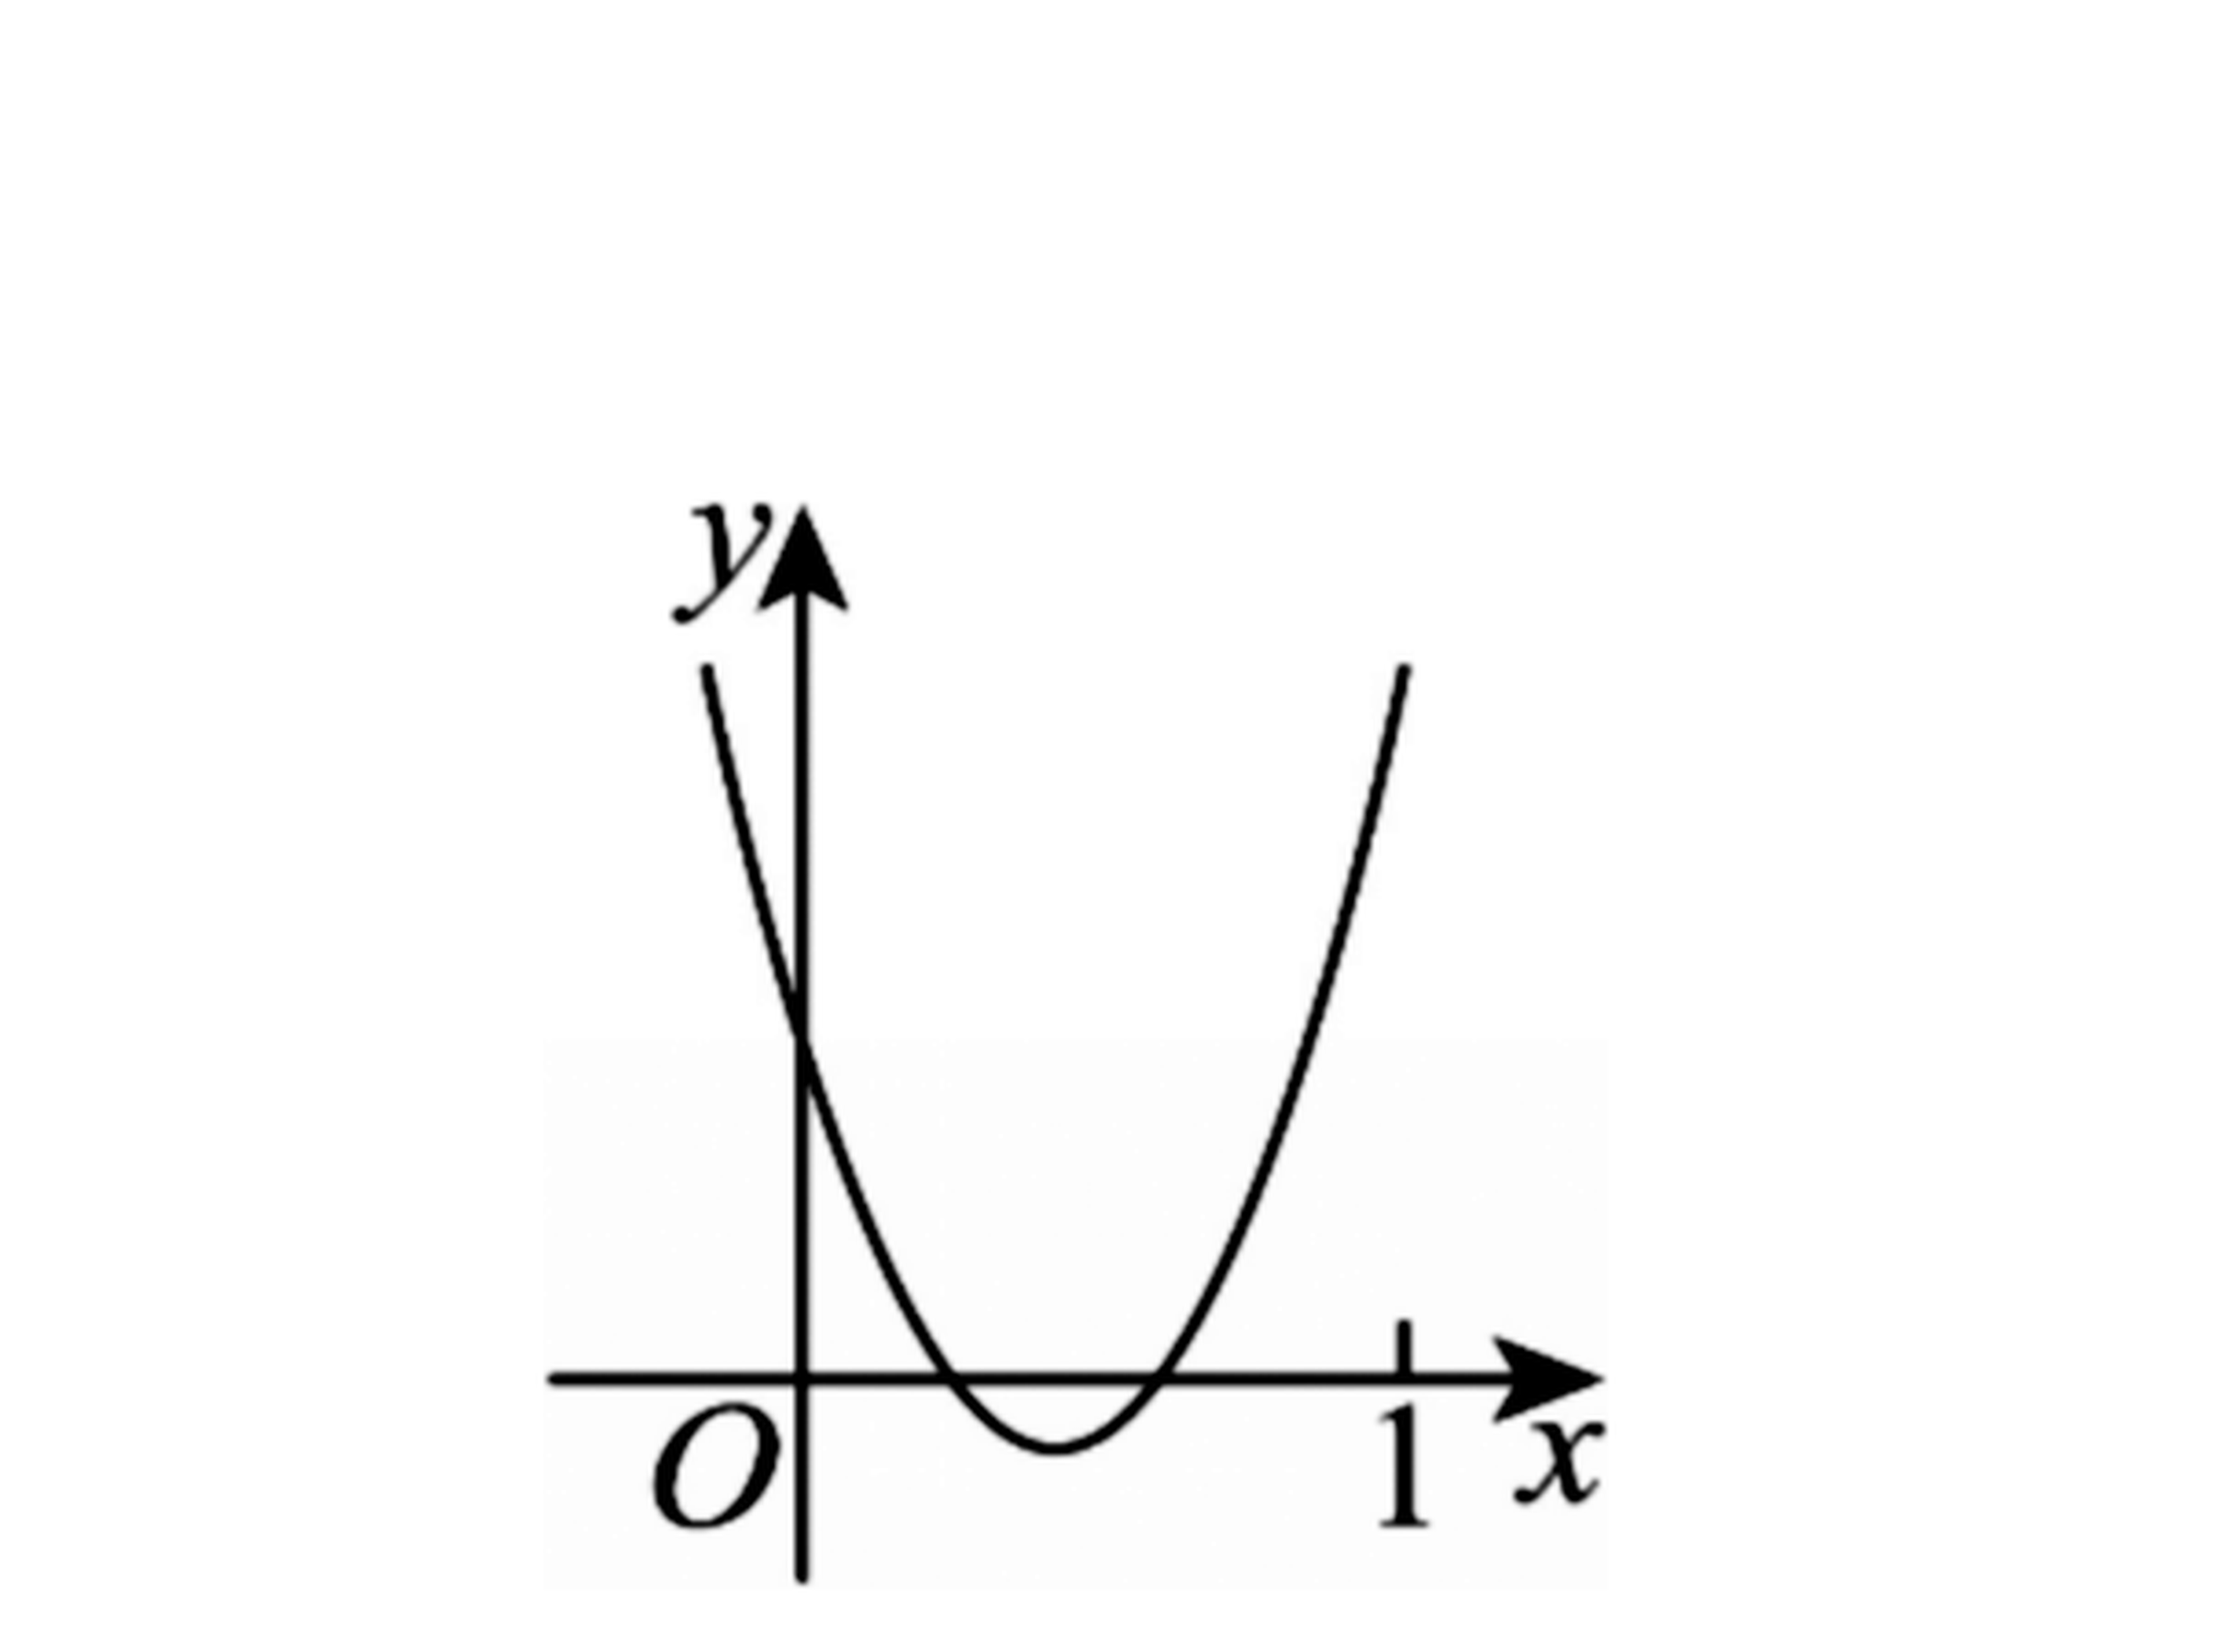
\includegraphics[width=0.32\textwidth]{figures/gao154_q15_stem.png}
\end{center}

\keepwithprev
\begin{center}
% 四幅指数函数图像选项取 05 页上半，按原卷 2×2 排布合并为一张，去粉色水印、去色、4× LANCZOS 放大；三版都出
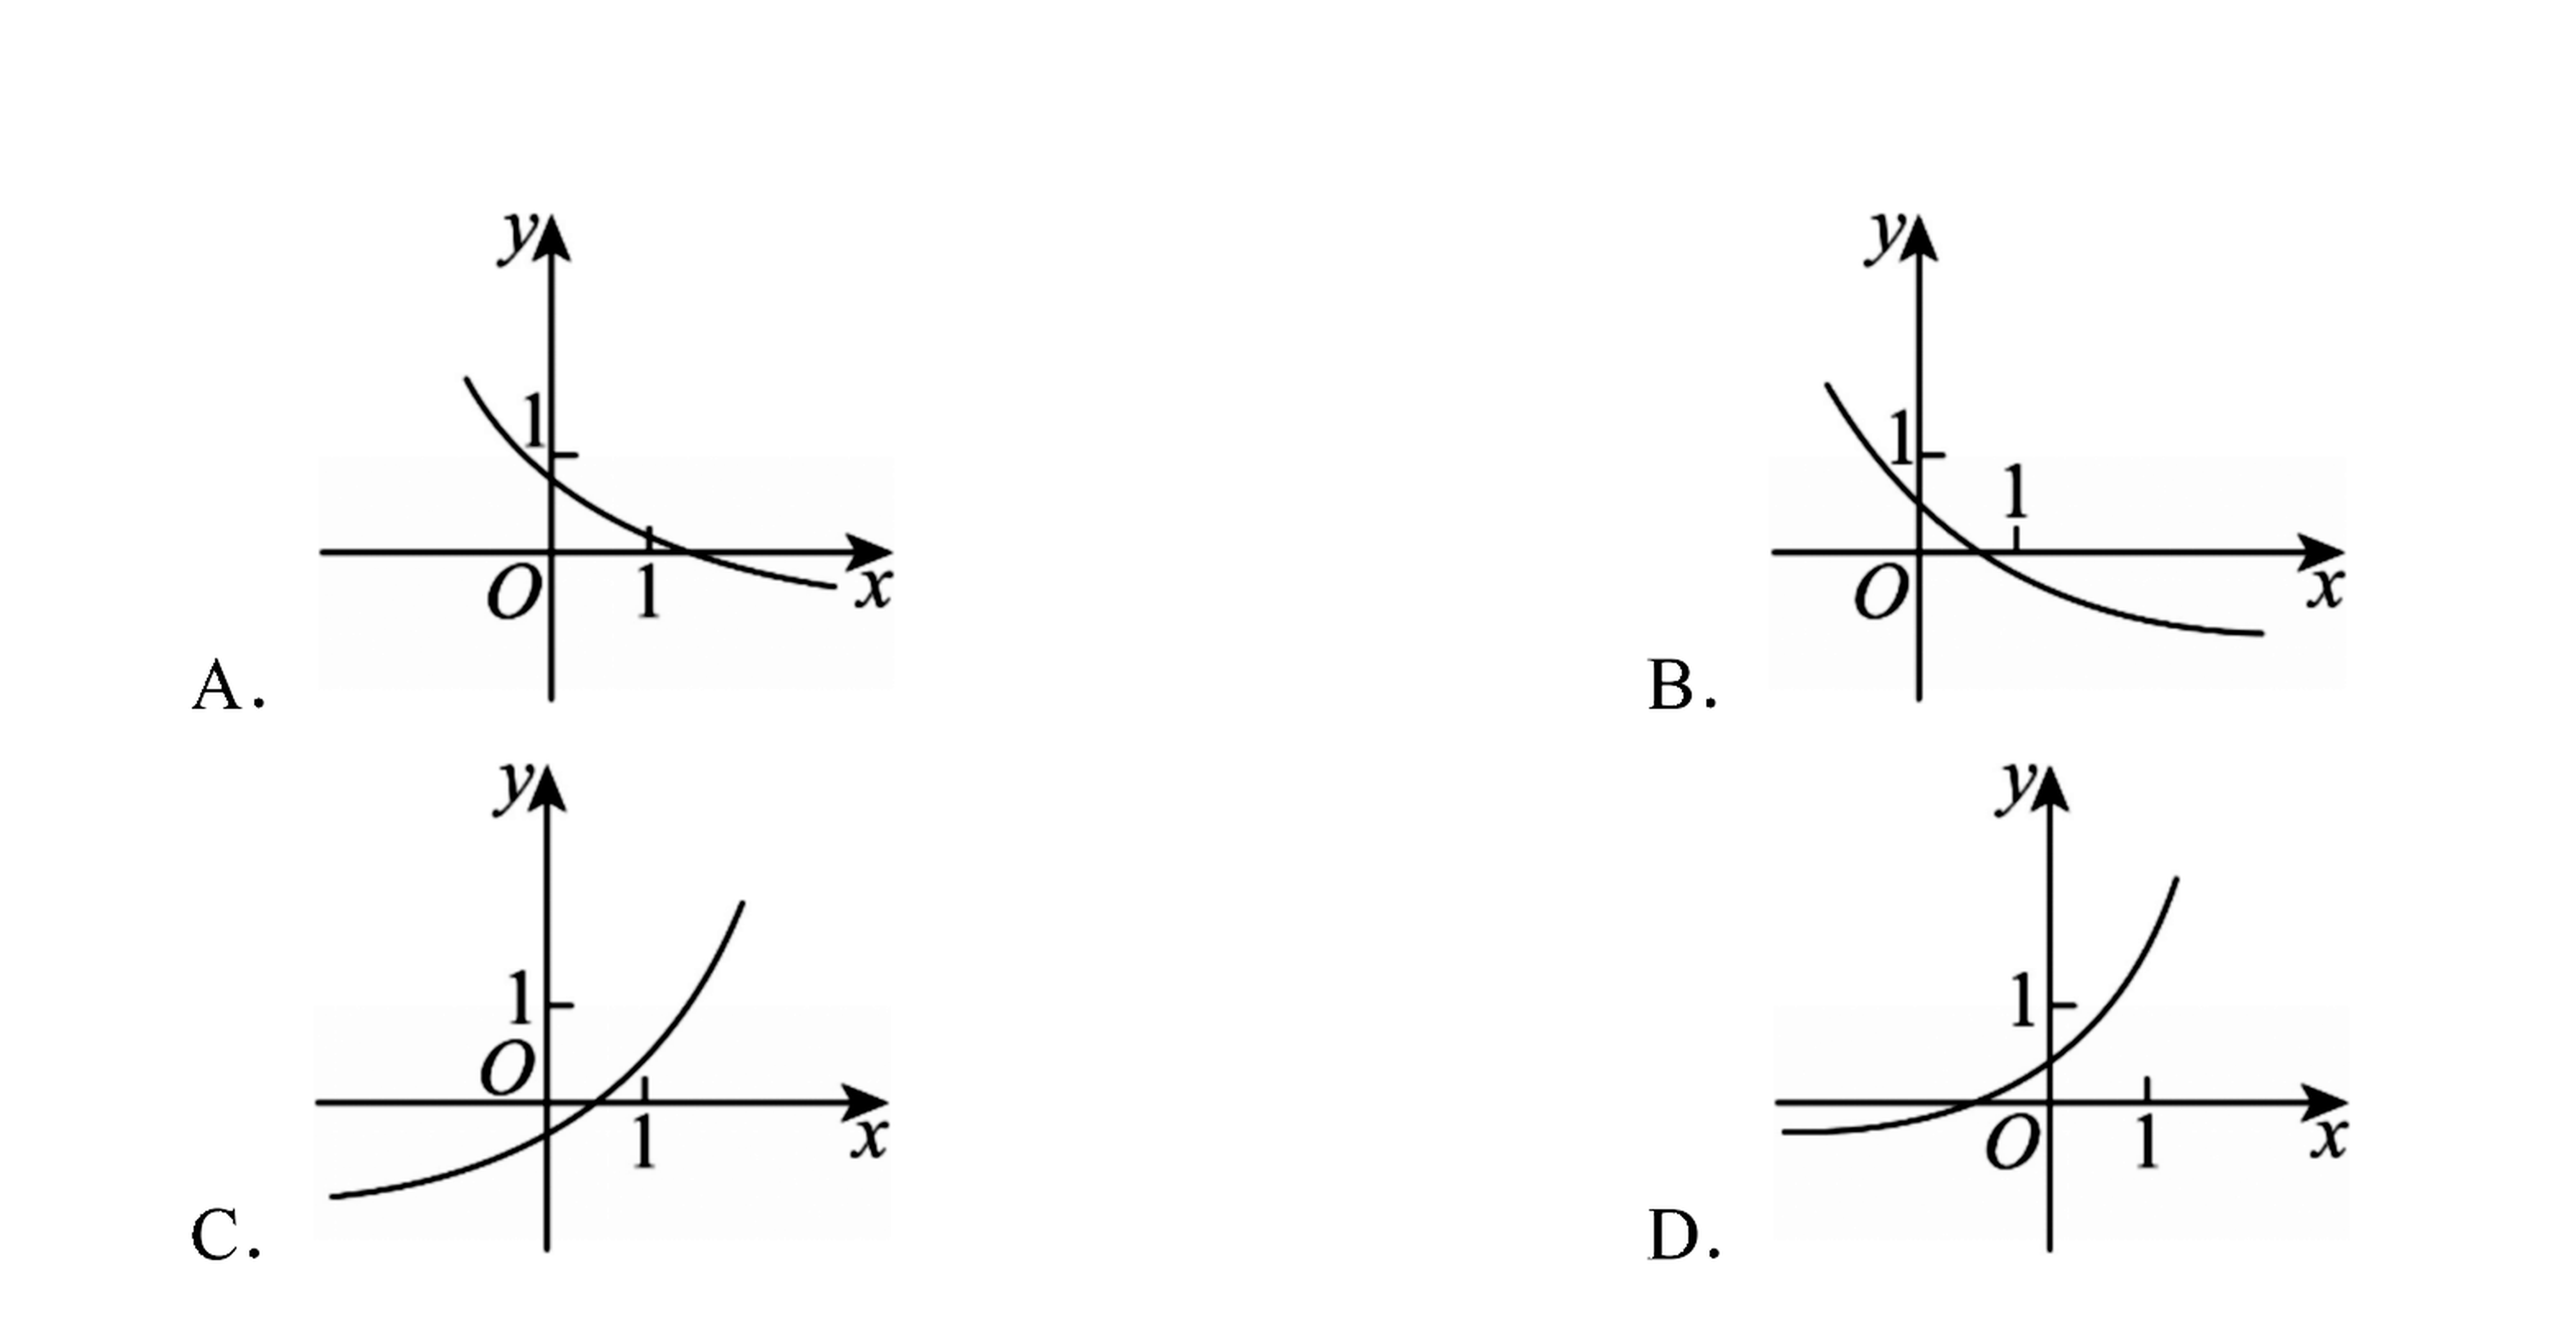
\includegraphics[width=0.80\textwidth]{figures/gao154_q15_opts.png}
\end{center}

\ifanswer
\solbegin
\step{由题意得 $0<a<b<1$，所以 $g(x)=a^x-b$ 在定义域 $\R$ 上严格减.}
\step{$g(0)=a^0-b=1-b>0$，$g(1)=a^1-b=a-b<0$，故 B 符合题意.}
\step{故选 $B$.}
\solend
\fi

% === Q16 === 高斯取整；解析 13 行，故选 C
\item 设 $[a]$ 表示不超过 $a$ 的最大整数，如 $[1.2]=1$，$[-3.2]=-4$，若 $x$、$y$、$z$ 为正实数，则 $\left[\dfrac{y+z}{x}\right]+\left[\dfrac{z+x}{y}\right]+\left[\dfrac{x+y}{z}\right]$ 的最小值为\mbox{（\quad）}

\keepwithprev
A. 2\qquad\qquad B. 3\qquad\qquad C. 4\qquad\qquad D. 6

\ifanswer
\solbegin
\step{若 $x$、$y$、$z$ 为正实数，}
\step{结合基本不等式得 $\dfrac{y+z}{x}+\dfrac{z+x}{y}+\dfrac{x+y}{z}=\dfrac yx+\dfrac xy+\dfrac zx+\dfrac xz+\dfrac zy+\dfrac yz$}
\step{$\geqslant2\sqrt{\dfrac yx\cdot\dfrac xy}+2\sqrt{\dfrac zx\cdot\dfrac xz}+2\sqrt{\dfrac zy\cdot\dfrac yz}=6$，当且仅当 $x=y=z$ 时取等号，}
\step{即 $\dfrac{y+z}{x}$，$\dfrac{z+x}{y}$，$\dfrac{x+y}{z}$ 中至少有一个不小于 2，不妨设 $\dfrac{y+z}{x}\geqslant\dfrac{z+x}{y}\geqslant\dfrac{x+y}{z}$，}
\step{$[a]$ 表示不超过 $a$ 的最大整数和 $\dfrac{y+z}{x}$，$\dfrac{z+x}{y}$，$\dfrac{x+y}{z}$ 中至少有一个不小于 2，}% 原卷此行把两句连写，照录未改（见 ⑤ 3）
\step{得 $\left[\dfrac{y+z}{x}\right]\geqslant2$，所以 $\left[\dfrac{y+z}{x}\right]+\left[\dfrac{z+x}{y}\right]+\left[\dfrac{x+y}{z}\right]\geqslant2$，}
\step{假设 $\left[\dfrac{y+z}{x}\right]+\left[\dfrac{z+x}{y}\right]+\left[\dfrac{x+y}{z}\right]$ 的最小值为 2，$\left[\dfrac{y+z}{x}\right]=2$，$\left[\dfrac{z+x}{y}\right]+\left[\dfrac{x+y}{z}\right]=0$，}
\step{所以 $2\leqslant\dfrac{y+z}{x}<3$，$0<\dfrac{z+x}{y}<1$，$0<\dfrac{x+y}{z}<1$，所以 $2<\dfrac{y+z}{x}+\dfrac{z+x}{y}+\dfrac{x+y}{z}<5$，}
\step{与 $\dfrac{y+z}{x}+\dfrac{z+x}{y}+\dfrac{x+y}{z}\geqslant6$ 矛盾，假设不成立，A 错误；}
\step{假设 $\left[\dfrac{y+z}{x}\right]+\left[\dfrac{z+x}{y}\right]+\left[\dfrac{x+y}{z}\right]$ 的最小值为 3，}
\step{则 $\left[\dfrac{y+z}{x}\right]=2$，$\left[\dfrac{z+x}{y}\right]=1$，$\left[\dfrac{x+y}{z}\right]=0$ 或 $\left[\dfrac{y+z}{x}\right]=3$，$\left[\dfrac{z+x}{y}\right]=\left[\dfrac{x+y}{z}\right]=0$，}
\step{同理可得 $3<\dfrac{y+z}{x}+\dfrac{z+x}{y}+\dfrac{x+y}{z}<6$，显然不成立，B 错误；}
\step{假设 $\left[\dfrac{y+z}{x}\right]+\left[\dfrac{z+x}{y}\right]+\left[\dfrac{x+y}{z}\right]$ 的最小值为 4，易得 $4<\dfrac{y+z}{x}+\dfrac{z+x}{y}+\dfrac{x+y}{z}<7$，}
\step{若取 $x=100$，$y=103$，$z=104$，则 $\left[\dfrac{y+z}{x}\right]=2$，$\left[\dfrac{z+x}{y}\right]=1$，$\left[\dfrac{x+y}{z}\right]=1$，}
\step{即 $\left[\dfrac{y+z}{x}\right]+\left[\dfrac{z+x}{y}\right]+\left[\dfrac{x+y}{z}\right]=4$，假设成立，C 正确，D 错误.}
\step{故选 $C$.}
\solend
\fi

\end{enumerate}

\bigsec{三、解答题}

\begin{enumerate}
\setcounter{enumi}{16}

% === Q17 === $B\subset A$ 单线照录；cases 块；解析 5 行
\item 设集合 $A=\{x\mid x^2+2x-3<0\}$，集合 $B=\{x\mid\lvert x+a\rvert<1\}$.

(1) 若 $a=3$，求 $A\cup B$；

(2) 设命题 $p:x\in A$，命题 $q:x\in B$，若 $p$ 是 $q$ 成立的必要不充分条件，求实数 $a$ 的取值范围.

\ifanswer
\solbegin
\step{(1) $A=(-3,1)$，}
\step{当 $a=3$ 时，$\lvert x+3\rvert<1$，解得 $-4<x<-2$，所以 $B=(-4,-2)$，}
\step{所以 $A\cup B=(-4,1)$.}
\step{(2) 因为 $p$ 是 $q$ 成立的必要不充分条件，所以 $B\subset A$.}
\step{因为 $A=(-3,1)$，$B=(-a-1,-a+1)$，所以 $\begin{cases}-a-1\geqslant-3\\-a+1<1\end{cases}$ 或 $\begin{cases}-a-1>-3\\-a+1\leqslant1\end{cases}$，解得 $0\leqslant a\leqslant2$.}
\solend
\fi

% === Q18 === 判别式 \Delta 两处照录；解析 9 行
\item 已知关于 $x$ 的一元二次方程 $x^2-mx+4m^2-3=0$ 的两个实根分别为 $x_1,x_2$.

(1) 若 $x_1,x_2$ 满足 $x_1+x_2=x_1x_2$，求实数 $m$ 的值；

(2) 求 $x_1^2+x_2^2$ 的最小值.

\ifanswer
\solbegin
\step{(1) 由韦达定理 $x_1+x_2=m$，$x_1x_2=4m^2-3$，}
\step{$\Delta=m^2-4(4m^2-3)=-15m^2+12\geqslant0$，即 $m^2\leqslant\dfrac45$.}
\step{由 $x_1+x_2=x_1x_2$ 得 $m=4m^2-3$，即 $4m^2-m-3=0$，}
\step{解得 $m=1$ 或 $m=-\dfrac34$.}
\step{$m=1$ 时 $m^2=1>\dfrac45$，$\Delta<0$，舍去；}
\step{$m=-\dfrac34$ 时 $m^2=\dfrac9{16}<\dfrac45$，符合，故 $m=-\dfrac34$.}
\step{(2) $x_1^2+x_2^2=(x_1+x_2)^2-2x_1x_2=m^2-2(4m^2-3)=-7m^2+6$，}
\step{函数 $y=-7m^2+6$ 开口向下，对称轴为 $m=0$，}% 原卷此处称求「最小值」，实为闭区间 $m^2\le\frac45$ 上的最小值，照录未改（见 ⑤ 4）
\step{故 $y_{\min}=-7\cdot\dfrac45+6=-\dfrac{28}{5}+\dfrac{30}{5}=\dfrac25$.}
\solend
\fi

% === Q19 === 全称命题；cases 块；解析 9 行
\item 设命题 $p$：对任意 $x\in\R$，不等式 $2mx^2+2mx+1>0$ 恒成立，$q:m\in\{m\mid\log_2(m-1)<1\}$.

(1) 若 $p$ 为真命题，求实数 $m$ 的取值范围；

(2) 若命题 $p$、$q$ 有且只有一个是真命题，求实数 $m$ 的取值范围.

\ifanswer
\solbegin
\step{(1) 由 $p$ 为真命题，得 $\forall x\in\R$，不等式 $2mx^2+2mx+1>0$ 恒成立，}
\step{当 $m=0$ 时，$1>0$ 恒成立；}
\step{当 $m\ne0$ 时，$\begin{cases}2m>0\\\Delta=4m^2-8m<0\end{cases}$，解得 $0<m<2$；}
\step{综上，$0\leqslant m<2$，即 $m$ 的取值范围是 $[0,2)$；}
\step{(2) 若 $q$ 为真，则有 $\log_2(m-1)<1$，得 $0<m-1<2$，解得 $1<m<3$，}
\step{因此命题 $q:m\in\{m\mid1<m<3\}$，由 (1) 得命题 $p:\{m\mid0\leqslant m<2\}$，}
\step{而命题 $p$、$q$ 有且只有一个是真命题，}
\step{当 $p$ 真 $q$ 假时，$\begin{cases}0\leqslant m<2\\m\leqslant1\text{ 或 }m\geqslant3\end{cases}$，解得 $0\leqslant m\leqslant1$，}
\step{当 $p$ 假 $q$ 真时，$\begin{cases}m<0\text{ 或 }m\geqslant2\\1<m<3\end{cases}$，解得 $2\leqslant m<3$，}
\step{故实数 $m$ 的取值范围是 $\{m\mid0\leqslant m\leqslant1\text{ 或 }2\leqslant m<3\}$.}
\solend
\fi

% === Q20 === Labubu 成本题；解析 10 行
\item Labubu 公司拟在 2027 年初推出智能机器人系列玩偶（单位：套）. 根据以往经验，其中一条生产线每月生产 $x$ 套玩具的成本 $P$ 由两部分费用（单位：元）构成：

(i) 固定成本（与生产玩具套数 $x$ 无关），总计 160000 元；

(ii) 每生产 $x$ 套需另投入的生产成本 $c(x)$ 元，其中 $c(x)=10x+\dfrac1{100}x^2$.

(1) 假设该生产线每月生产出的玩具能全部售出，问：该生产线每月生产玩具多少套时，可使得平均每套所需成本费用最少？此时每套玩具的成本费用是多少？

(2) 假设该生产线每月生产出的玩具能全部售出，但随着 $x$ 的增大，每月生产所需的直接总成本在急剧增加，因此售价也需随着 $x$ 的增大而适当增加. 设每套玩具的售价为 $q(x)$ 元，$q(x)=a+\dfrac xb$（$a,b\in\R$）. 若当月产量为 10000 套时利润最大，此时每套售价为 150 元，试求 $a,b$ 的值.（利润=销售收入$-$成本费用）

\ifanswer
\solbegin
\step{(1) 每月总成本 $P=160000+10x+\dfrac1{100}x^2$，}
\step{平均每套成本为 $\dfrac Px=\dfrac{160000}{x}+10+\dfrac x{100}\geqslant10+2\sqrt{\dfrac{160000}{x}\cdot\dfrac x{100}}=90$.}
\step{等号成立当且仅当 $\dfrac{160000}{x}=\dfrac x{100}$ 时，即 $x=4000$ 时取等号，}
\step{所以每月生产 4000 套时平均每套成本最少，此时每套成本为 90 元.}
\step{(2) 利润 $W(x)=x\cdot q(x)-P=\left(\dfrac1b-\dfrac1{100}\right)x^2+(a-10)x-160000$.}
\step{要在 $x=10000$ 处取得最大值，需 $\dfrac1b-\dfrac1{100}<0$，且对称轴为 $x=10000$，}
\step{故 $-\dfrac{a-10}{2\left(\frac1b-\frac1{100}\right)}=10000$，即 $a-10=-20000\left(\dfrac1b-\dfrac1{100}\right)$.}
\step{又 $q(10000)=a+\dfrac{10000}{b}=150$.}
\step{令 $t=\dfrac1b$，则 $a=150-10000t$，}
\step{代入上式 $140-10000t=-20000t+200$，解得 $t=\dfrac3{500}$，即 $b=\dfrac{500}{3}$；}
\step{再由 $a=150-10000\times\dfrac3{500}=150-60=90$，所以 $a=90$，$b=\dfrac{500}{3}$.}
\solend
\fi

% === Q21 === $A^+$／$A^-$ 新定义；$A\subseteq$ 带下划线照录、\varnothing；解析 16 行
\item 设集合 $A$ 为非空数集，定义 $A^+=\{x\mid x=a+b,a,b\in A\}$，$A^-=\{x\mid x=\lvert a-b\rvert,a,b\in A\}$.

(1) 若集合 $A=\{-1,1\}$，写出集合 $A^+$ 及 $A^-$；

(2) 若集合 $A=\{x_1,x_2,x_3,x_4\}$，$x_1<x_2<x_3<x_4$，且 $A^-=A$，求证：$x_1+x_4=x_2+x_3$；

(3) 若集合 $A\subseteq\{x\mid0\leqslant x\leqslant2020,x\in\N\}$，且 $A^+\cap A^-=\varnothing$，求集合 $A$ 元素的个数的最大值.

\ifanswer
\solbegin
\step{(1) 由 $A=\{-1,1\}$，得 $A^+=\{-2,0,2\}$，$A^-=\{0,2\}$；}
\step{(2) 由于集合 $A=\{x_1,x_2,x_3,x_4\}$，$x_1<x_2<x_3<x_4$，且 $A^-=A$，}
\step{所以 $A^-$ 中也只包含四个元素，即 $A^-=\{0,x_2-x_1,x_3-x_1,x_4-x_1\}$，}
\step{剩下的 $x_3-x_2=x_4-x_3=x_2-x_1$，所以 $x_1+x_4=x_2+x_3$；}
\step{(3) 设 $A=\{a_1,a_2,\cdots,a_k\}$ 满足题意，其中 $a_1<a_2<\cdots<a_k$，}
\step{则 $2a_1<a_1+a_2<a_1+a_3<\cdots<a_1+a_k<a_2+a_k<a_3+a_k<\cdots<a_{k-1}+a_k<2a_k$，所以 $\lvert A^+\rvert\geqslant2k-1$，}
\step{且 $a_1-a_1<a_2-a_1<a_3-a_1<\cdots<a_k-a_1$，所以 $\lvert A^-\rvert\geqslant k$，}
\step{因为 $A^+\cap A^-=\varnothing$，所以 $\lvert A^+\cup A^-\rvert=\lvert A^+\rvert+\lvert A^-\rvert\geqslant3k-1$，}
\step{$A^+\cup A^-$ 中最小的元素为 0，最大的元素为 $2a_k$，所以 $\lvert A^+\cup A^-\rvert\leqslant2a_k+1$，}
\step{所以 $3k-1\leqslant2a_k+1\leqslant4041$（$k\in\N^*$），所以 $k\leqslant1347$，}
\step{实际上当 $A=\{674,675,676,\cdots,2020\}$ 时满足题意，证明如下：}
\step{设 $A=\{m,m+1,m+2,\cdots,2020\}$，$m\in\N$，}
\step{则 $A^+=\{2m,2m+1,2m+2,\cdots,4040\}$，$A^-=\{0,1,2,\cdots,2020-m\}$，}
\step{由题意得 $2020-m<2m$，即 $m>673\dfrac13$，}
\step{故 $m$ 的最小值为 674，于是当 $m=674$ 时，$A$ 中元素最多，}
\step{即 $A=\{674,675,676,\cdots,2020\}$ 时满足题意，}
\step{综上所述，集合 $A$ 中元素的个数的最大值是 1347.}
\solend
\fi

\end{enumerate}

\bigsec{附加题}

\begin{enumerate}

% === 附加题 1 === 另起编号 1；「n 元集和集」弯引号；解析 6 行
\item 设集合 $A=\{a_1,a_2,a_3,a_4\}$，$C=\{2,3,4,6\}$，新定义：集合 $A$ 中所有含 $n$ 个元素的子集中 $n$ 个元素之和的不同值组成的集合为“$n$ 元集和集”. 若 $A$ 的“3 元集和集”为 $C$，则集合 $A=$\blankline[4.4em].

\ifanswer
\solbegin
\step{集合 $A$ 的 3 元子集共有 4 个：$\{a_1,a_2,a_3\}$，$\{a_1,a_2,a_4\}$，$\{a_1,a_3,a_4\}$，$\{a_2,a_3,a_4\}$，}
\step{集合 $C=\{a_1+a_2+a_3,a_1+a_2+a_4,a_1+a_3+a_4,a_2+a_3+a_4\}$，}
\step{不妨令 $a_1<a_2<a_3<a_4$，}
\step{则 $a_1+a_2+a_3<a_1+a_2+a_4<a_1+a_3+a_4<a_2+a_3+a_4$，}
\step{而 $C=\{2,3,4,6\}$，因此 $\begin{cases}a_1+a_2+a_3=2\\a_1+a_2+a_4=3\\a_1+a_3+a_4=4\\a_2+a_3+a_4=6\end{cases}$，相加化简得 $a_1+a_2+a_3+a_4=5$，}
\step{解得 $a_1=-1$，$a_2=1$，$a_3=2$，$a_4=3$，所以 $A=\{-1,1,2,3\}$.}
\solend
\fi

% === 附加题 2 === 解析配图（仅答案版出）；四选项；解析 15 行，故选 A
\item 已知函数 $f(x)=\log_p x+q$，其中 $p>0$ 且 $p\ne1$，曲线 $y=f(x)$ 经过 $P(1,2)$、$Q(2,3)$ 两点. 设 $g(x)=f(x)\cdot[f(x)-2]$，若 $\lvert g(a)\rvert=\lvert g(b)\rvert=\lvert g(c)\rvert=\lvert g(d)\rvert$，且 $a<b<c<d$，则 $ad(b+c)$ 的取值范围为\mbox{（\quad）}

\keepwithprev
A. $\left(\dfrac14,\dfrac5{16}\right)$\qquad B. $\left(\dfrac18,\dfrac5{16}\right)$\qquad C. $\left(\dfrac14,\dfrac25\right)$\qquad D. $\left(\dfrac18,\dfrac25\right)$

\ifanswer
\solbegin
\step{函数 $f(x)=\log_p x+q$，且曲线 $y=f(x)$ 经过点 $P(1,2)$ 和 $Q(2,3)$，}
\step{所以 $\begin{cases}f(1)=q=2\\f(2)=\log_p2+q=3\end{cases}$，解得 $p=2$，$q=2$，$f(x)=\log_2 x+2$.}
\step{不妨设 $\lvert g(x)\rvert=k$，令 $\log_2 x=m$，则 $f(x)\cdot[f(x)-2]=m(m+2)=m^2+2m$，}
\step{画出函数 $y=\lvert m^2+2m\rvert$ 的图象，如图所示，}
\begin{center}
% $y=|m(m+2)|$ 图像取 11 页右上，去粉色水印、去色、4× LANCZOS 放大；仅答案版出
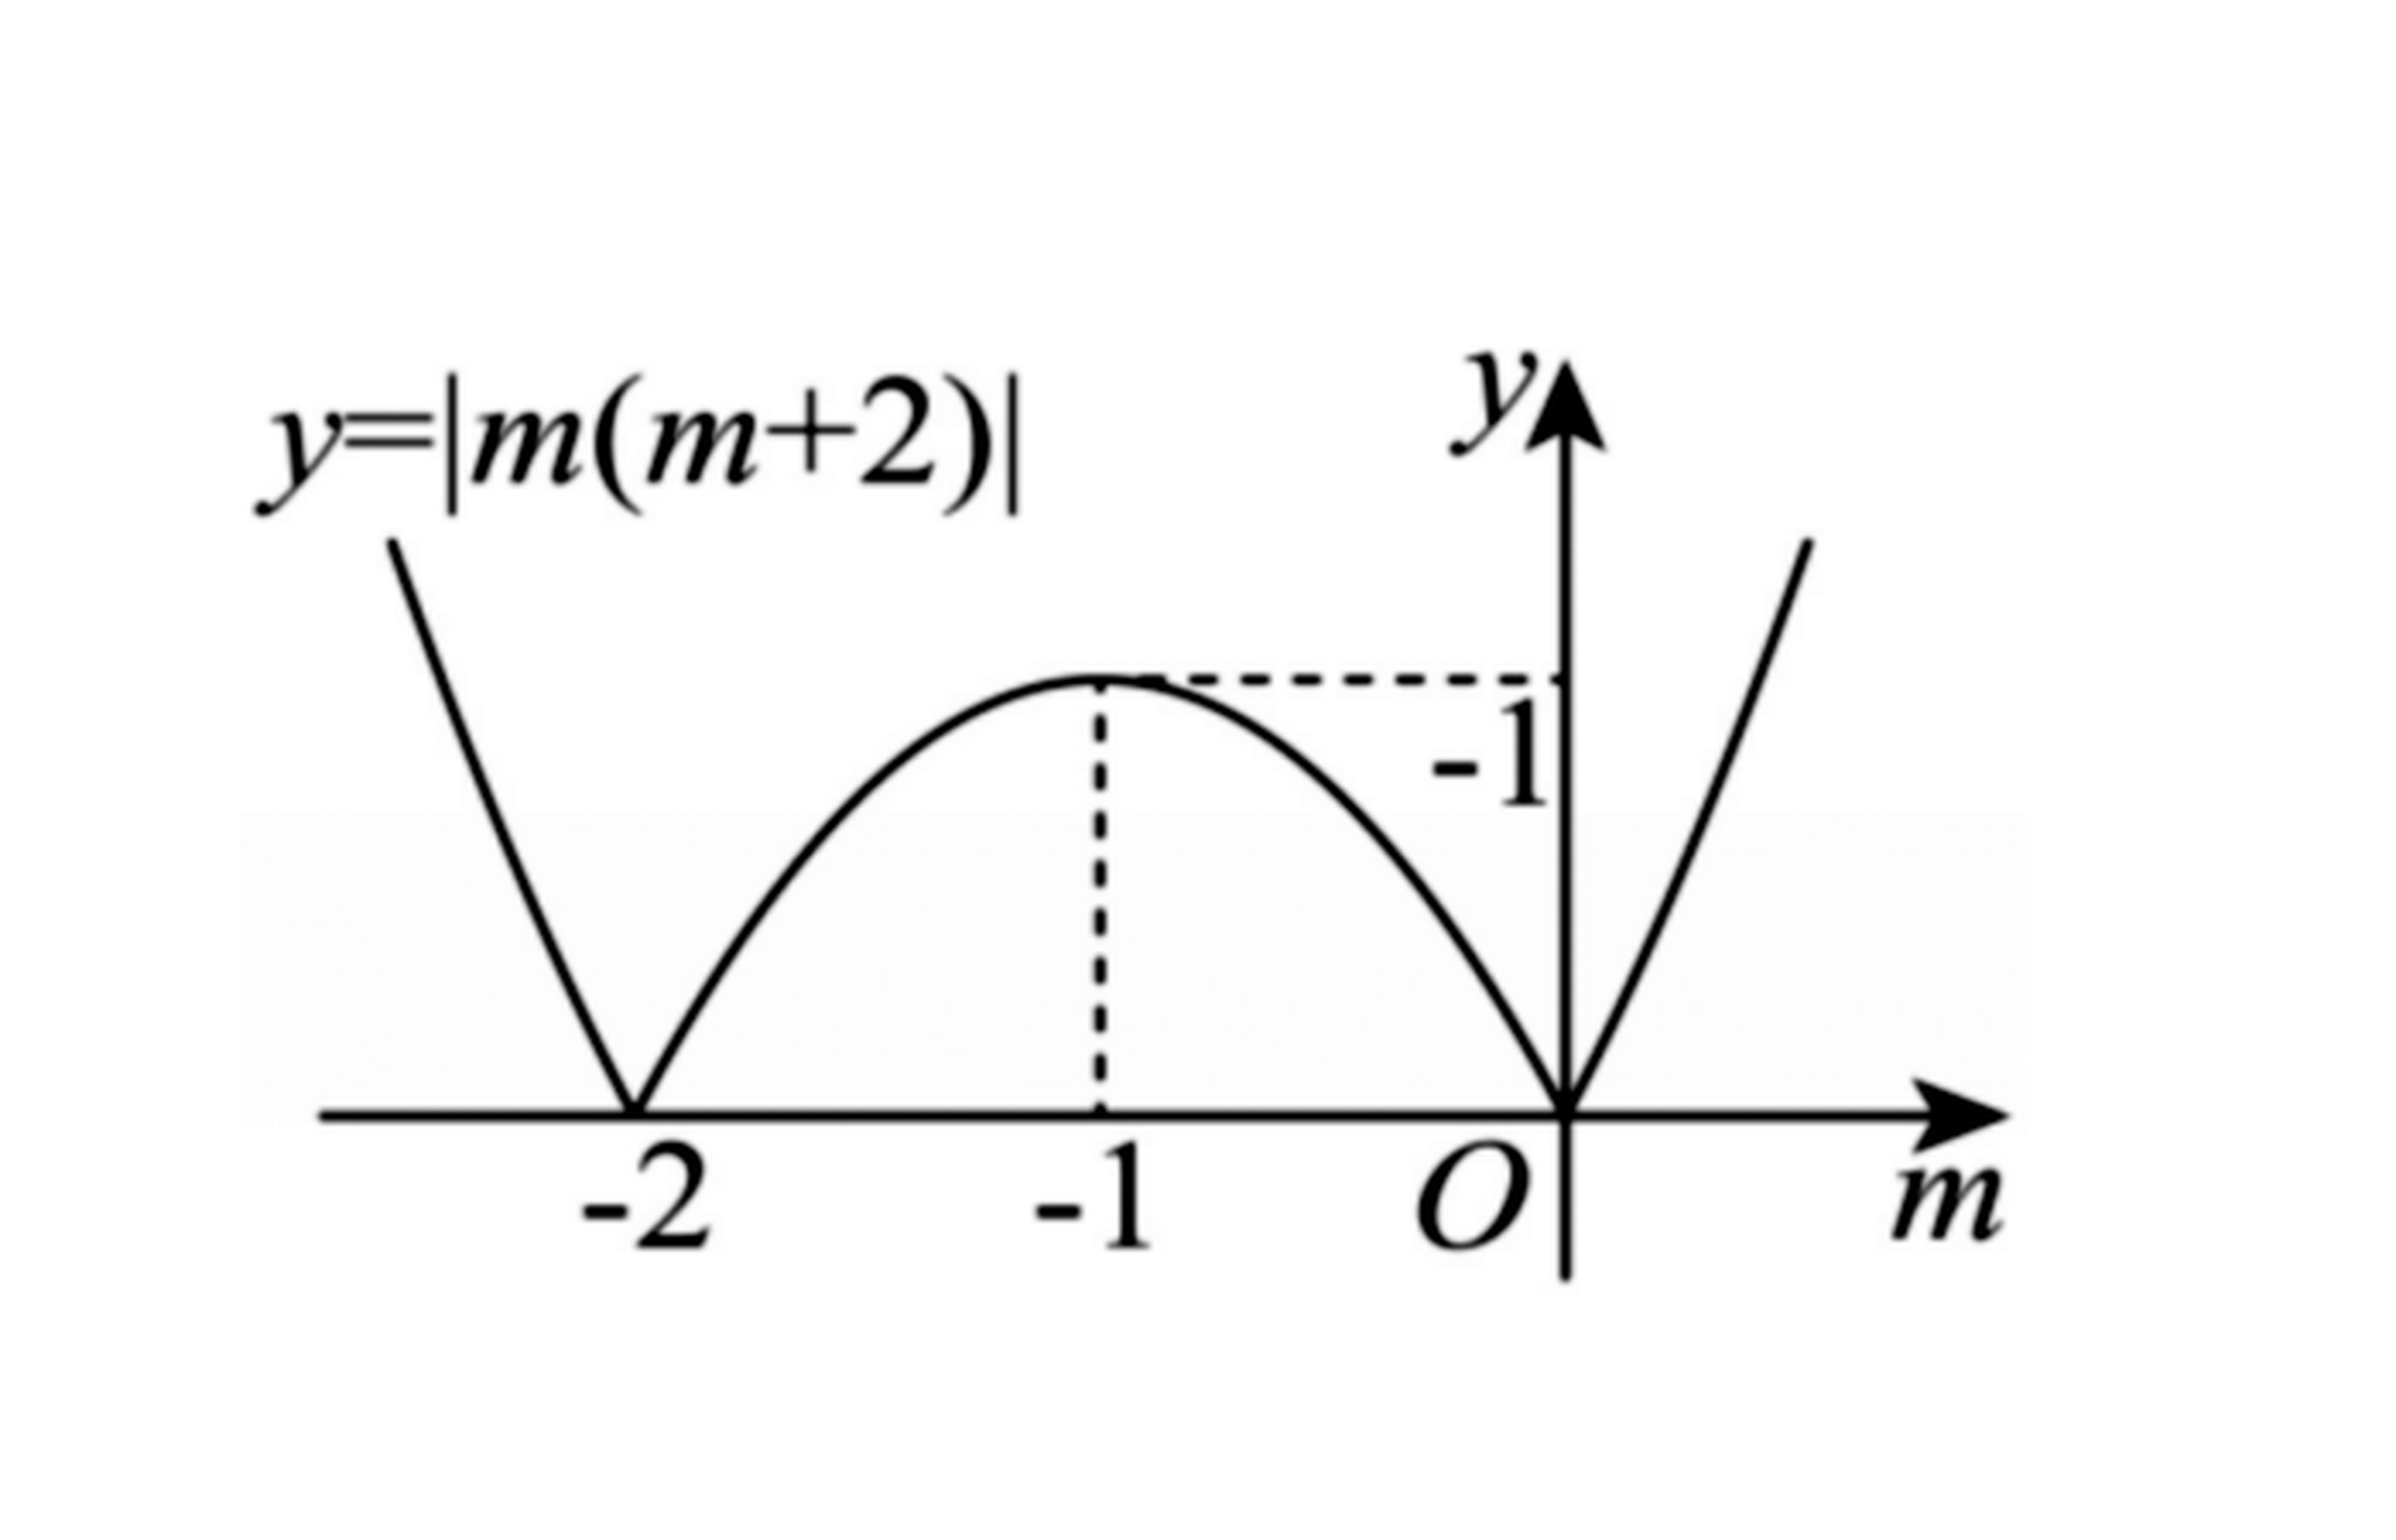
\includegraphics[width=0.46\textwidth]{figures/gao154_fujia2.png}
\end{center}
\step{由图像得 $k\in(0,1)$，}
\step{所以方程 $m^2+2m=k$ 和 $m^2+2m=-k$ 各有两个不同的根，}
\step{其中方程 $m^2+2m-k=0$ 的两根为 $m=-1\pm\sqrt{1+k}$，}
\step{方程 $m^2+2m+k=0$ 的两根为 $m=-1\pm\sqrt{1-k}$，}
\step{所以 $m_1=-1-\sqrt{1+k}$，$m_2=-1-\sqrt{1-k}$，$m_3=-1+\sqrt{1-k}$，$m_4=-1+\sqrt{1+k}$，且 $m_1<m_2<m_3<m_4$，}
\step{由 $m=\log_2 x$，则 $x=2^m$，}
\step{所以 $a=2^{-1-\sqrt{1+k}}$，$b=2^{-1-\sqrt{1-k}}$，$c=2^{-1+\sqrt{1-k}}$，$d=2^{-1+\sqrt{1+k}}$，}
\step{所以 $ad=2^{-1-\sqrt{1+k}}\times2^{-1+\sqrt{1+k}}=2^{(-1-\sqrt{1+k})+(-1+\sqrt{1+k})}=2^{-2}=\dfrac14$，}
\step{$b+c=2^{-1-\sqrt{1-k}}+2^{-1+\sqrt{1-k}}=\dfrac{2^{-\sqrt{1-k}}+2^{\sqrt{1-k}}}{2}$，}
\step{令 $s=\sqrt{1-k}$，其中 $s\in(0,1)$，则 $b+c=\dfrac12\left(2^{-s}+2^s\right)$，}
\step{设函数 $y=2^s+\dfrac1{2^s}$，令 $r=2^s\in(1,2)$，所以 $y=r+\dfrac1r$ 在 $(1,2)$ 上严格增，}
\step{所以函数 $y=2^s+\dfrac1{2^s}$ 在 $(0,1)$ 上严格增，所以 $y=2^s+\dfrac1{2^s}\in\left(2,\dfrac52\right)$，}
\step{所以 $b+c=\dfrac{2^{-s}+2^s}{2}\in\left(1,\dfrac54\right)$，$ad(b+c)=\dfrac{b+c}{4}\in\left(\dfrac14,\dfrac5{16}\right)$，}
\step{所以 $ad(b+c)$ 的取值范围是 $\left(\dfrac14,\dfrac5{16}\right)$，故选 $A$.}
\solend
\fi

\end{enumerate}

\end{document}
"
% 紧凑版：xelatex "\def\iscompact{1}% 高一154_徐汇中学_期中.tex
%   —— 高一上数学"2026-2027 年徐汇中学高一上期中"（试卷版/答案版/紧凑版）
% 试卷版：xelatex 高一154_徐汇中学_期中.tex
% 答案版：xelatex "\def\isanswer{1}\input{高一154_徐汇中学_期中.tex}"
% 紧凑版：xelatex "\def\iscompact{1}\input{高一154_徐汇中学_期中.tex}"
%
% ① 原始材料：微信公众号"魔都数学加油站"文章，连载"27学年高一154"，原文标题
% "27学年高一154——2026-2027年上海市徐汇中学高一上期中"；
% 原文链接：https://mp.weixin.qq.com/s/Qs2T7Zwsug-KKFE2wefDUg 。
% 正文为 12 张 PNG 页（01/03/04/05/07/11/12 为 2560×3620，
% 02/06/08/09/10 为 4762×6735，同一篇各页分辨率混排，逐页按各自分辨率裁图核对）。
% 体例：讲评版——一、填空题 3—12（10 题）、二、选择题 13—16（4 题）、
% 三、解答题 17—21（5 题）、附加题 1—2（2 题，原卷**另起编号**"1." "2."，
% 不与正题连号，同 高一a 成例），共 21 题；全卷每题均印【解析】
% （逐题核实，见 ② ②）。题目、答案、解析均据原图转录；卷面粉红色水印
% "魔都数学加油站"及公众号页脚未录入。
% 全卷插图清单（逐页通读 12 页确认）：3 组——
%   · Q15 题干配图（$f(x)=(x-a)(x-b)$ 抛物线，04 页右下：x/y 轴、O、1、
%     开口向上两零点均在 (0,1) 内），三版都出，裁 figures/gao154_q15_stem.png；
%   · Q15 四幅图像选项（05 页上半 2×2 排布，A/B/C/D 四幅指数函数图像，
%     合并成一张，照 高一136 Q13/Q22 成例），三版都出，
%     裁 figures/gao154_q15_opts.png；
%   · 附加题第 2 题解析配图（$y=\lvert m(m+2)\rvert$ 图像，11 页右上：
%     W 形折线、$-2$、$-1$、O、虚线 $y=1$ 与 $m=-1$），仅答案版出，
%     裁 figures/gao154_fujia2.png；
%   3 图均取自原卷截图，去粉色水印、去色、4× LANCZOS 放大；Q15 题干图
%   左侧题干残字"的图"已裁白。其余各页逐页确认无其它题目配图、无表格；
%   12 页下半仅水印、无正文。
%
% 卷首标题：原卷印作"2026-2027 年徐汇中学高一上期中"，年份区间按全稿惯例排 en dash；
% 原卷卷面未印副标题，本稿按同期中卷知识模块口径补出"集合与常用逻辑用语、不等式、函数"。
%
% ② 与原卷的排版差异：
%   ① 原文从第 3 题起，本稿保留原题号；共 21 题四节，正题到 21，附加题另起编号
%      1—2（\bigsec{附加题} 后 \begin{enumerate} 不 \setcounter，同 高一a 成例）；
%   ② 全 21 题均印【解析】、用 \solbegin…\solend，无只印【答案】或答案印括号内的题；
%      四道正题选择题答案在解析末句"故选 C／A／B／C"（Q13—Q16）、附加题第 2 题
%      答案在解析末句"故选 A"，括号 \mbox{（\quad）} 留空、不另提 \ans{}；
%      答案版【答案】/【解析】标记数 = 21 = 全卷题数；
%   ③ 原卷卷面未印副标题，本稿按知识模块口径补出；
%   ④ 原卷填空横线按全稿惯例排 \blankline[4.4em]；选择题括号排 \mbox{（\quad）}、
%      四道正题选择题与附加题第 2 题的选项段前按惯例各加 \keepwithprev
%      （Q15 与附加题 2 的选项段是整块图，\keepwithprev 后接 \begin{center}）；
%      解答题不留作答区、不加 \anspace（原卷为讲评版）；
%   ⑤ 数集黑板粗体：Q4"$x,y\in R$"、Q9"$x\in\R$"、Q13 无、
%      Q15"定义域 $\R$"、Q19"$\forall x\in\R$"、Q21"$x\in\N$"与"$k\in\N^*$"、
%      Q20"$a,b\in\R$"、附加题 2 无——原卷印斜体或正体粗体 R/N/N*，
%      按全稿惯例归一 \R／\N／\N^*；绝对值排 \lvert…\rvert
%      （Q5、Q9、Q12、Q13、Q16、Q21、附加题 2），集合描述竖线排 \mid
%      （Q5、Q17、Q19、Q21），不等号按全稿惯例排 \leqslant／\geqslant；
%      空集 \varnothing（Q21 题干 (3)）；
%   ⑥ 子集符号逐处照录、不得统一：Q6 题干印"$\{1,2\}\subset M\subseteq\{1,2,3,4,5\}$"
%      （前单线 ⊂、后带下划线 ⊆，同句两形并用），解析亦两形并用；
%      Q17 解析 (2)"$B\subset A$"印单线 ⊂；Q21 题干 (3)"$A\subseteq\{x\mid\cdots\}$"
%      印带下划线 ⊆——逐处放大核，分别 \subset／\subseteq，照录未统一（见 ④）；
%   ⑦ 判别式 Δ/△：Q18 解析 (1)"$\Delta=m^2-4(4m^2-3)$"与 Q19 解析 (1)
%      "$\Delta=4m^2-8m<0$"两处均印等腰偏高粗三角、照录 \Delta；本卷无扁等边
%      细线 \triangle 用例（见 ④）；
%   ⑧ 中文弯引号照录：Q4"设 $x$、$y\in\R$. 若 $x+y>2$，则 $x>1$ 或 $y>1$"、
%      附加题 1"$n$ 元集和集"与"3 元集和集"；注释里一律 ASCII 引号；
%      数学式内 CJK 用 \text{}（Q5 解集描述"或"、Q19 集合描述的"或"）；
%   ⑨ "图像／图象"逐处放大核：Q15 题干与解析印"图象"（象，无亻）、
%      Q16 无、附加题 2 解析印"图象"与"图像"（"画出函数…的图象"、
%      "由图像得"——两形并用，逐处照录未统一）；Q13/Q14 无数集图像字样；
%      半角逗号在数学组之间是全稿惯例、非笔误，逐处照录（Q3、Q10、Q16、
%      Q18、Q20、Q21 的 $x_1,x_2$ 之类）；行末西文句点 ASCII `.`；
%      行中全角逗号／顿号照录（Q6"3，4，5"、Q20"（单位：元）"、
%      附加题 1"$a_1,a_2,a_3,a_4$"）；
%   ⑩ 复杂式照录别简化：Q3 $a^{\frac{12}{7}}\cdot\left(\frac17\right)^{\frac17}
%      \cdot\sqrt[7]{a^4}$ 与 $7^{-\frac17}a^{\frac{16}{7}}$、Q7 $x^{-m}$、
%      Q8 $\frac{b-2a+2}{2a}$、Q11 $\frac{9+4\sqrt2}{6}$、Q12 $506\frac29$ 与
%      $506\frac49$、Q16 高斯取整 $[a]$、Q20 $c(x)=10x+\frac1{100}x^2$ 与
%      $q(x)=a+\frac xb$、Q21 $A^+$／$A^-$ 与 $|A^+|\geqslant2k-1$、
%      附加题 2 $m=-1\pm\sqrt{1+k}$ 与 $ad(b+c)$；
%      \left…\right 不得拆到不同 $…$ 组（Q5 $\left\{x\mid\cdots\right\}$、
%      Q20 $\left(\frac1b-\frac1{100}\right)$、附加题 2 $\left(\frac14,\frac5{16}\right)$）；
%      cases 块一律 \begin{cases}…\end{cases}；
%   ⑪ 一条 \step = 原卷解析的一个印刷行，cases 块整体算一个印刷行；别并折行、
%      别拆行。Q11 九行、Q12 六行、Q16 十六行、Q20 十一行、Q21 十七行、
%      附加题 2 十八行均按印刷行逐条断，不丢行；
%   ⑫ 配图：Q15 题干小图（三版都出）放 \item 内题干之后 \begin{center}，
%      Q15 四幅选项图（三版都出）放 \keepwithprev 之后的 \begin{center}，
%      Q15 用 \needvspace 守卫把"题干＋两图"整块推走（守卫放 \item 之前，
%      见 高一145 Q14/Q20 与 高一136 Q13 成例）；附加题 2 解析配图（仅答案版出）
%      放 \ifanswer 内 \solbegin…\solend 的 \step 之间（高一73 第 16 题成例）；
%   ⑬ 原卷解析内无红色"法一／法二"之类小标题，故本卷无 \stepm；红色水印
%      "魔都数学加油站"不录入；
%   ⑭ 跨页续印按题合并：见 ⑥；
%
% ③ 行数复核：一条 \step = 原卷解析的一个印刷行，cases 块作一个印刷行计。
%   逐题数（主会话逐页核对定稿）：Q3：1；Q4：1；Q5：3；Q6：4；Q7：3；
%   Q8：1；Q9：5；Q10：4；Q11：9；Q12：6；Q13：5；Q14：4；Q15：3；
%   Q16：16；Q17：5；Q18：9；Q19：10；Q20：11；Q21：17；
%   附加题 1：6；附加题 2：18。
%   合计 141 条 \step（本卷无 \stepm），与原卷逐题印刷行相等。全卷 21 题
%   均设 \solbegin…\solend，答案版【答案】/【解析】标记数 = 21 = 全卷题数。
%
% ④ 判别式／子集符号结论（逐处放大原图照录、不得统一，主会话像素级复核）：
%   判别式：Q18 解析 (1)"$\Delta=m^2-4(4m^2-3)=-15m^2+12\geqslant0$"、
%      Q19 解析 (1)"$\Delta=4m^2-8m<0$"共 2 处，逐处放大确认印等腰偏高
%      粗三角（高>宽、右斜边粗），照录 \Delta；本卷无扁等边细线 \triangle
%      用例，无几何三角形符号。
%   子集：Q6 题干"$\{1,2\}\subset M\subseteq\{1,2,3,4,5\}$"前 ⊂ 单线、
%      后 ⊆ 带下划线（/tmp/gao154/z/zoom/q6_subset.png），解析两处同样两形
%      并用，分别照录 \subset／\subseteq；Q17 解析 (2)"$B\subset A$"单线
%      照录 \subset；Q21 题干 (3)"$A\subseteq\{x\mid\cdots\}$"带下划线
%      照录 \subseteq。本卷 ⊂ 与 ⊆ 混用逐处照录、不得统一。
%      空集 \varnothing（Q21 题干 (3)）、数集 \R／\N／\N^* 归一见 ② ⑤。
%
% ⑤ 存疑照录（放大原图确认，照录未改、正文对应处另有 % 注）：
%   1. Q7 题干印 $f(x)=(3m-1)x^{-m}$，解析首句却写"幂函数 $f(x)=x^\alpha$
%      的系数必须为 1"（用 $\alpha$ 作指数记号），随后 $f(2)=2^\alpha=8$
%      得 $\alpha=3$、$f(x)=x^3$——题干指数 $-m$ 与解析 $\alpha$ 记法不同，
%      系原卷记号前后不一，逐处照录未统一（放大 01/02 页确认）。
%   2. Q11 解析"因为 $u>0,v>0$，由基本不等式得 $\frac{4v}{u}+\frac{2u}{v}
%      \geqslant2\sqrt{\frac{4v}{u}\cdot\frac{2u}{v}}=4\sqrt2$"与
%      "所以 $\frac4u+\frac1v=\frac16\left(\frac4u+\frac1v\right)(2u+v)$"
%      照录，未把 $u,v$ 化简回 $x,y$。
%   3. Q16 解析把"$[a]$ 表示不超过 $a$ 的最大整数"与"和至少有一个不小于 2"
%      连写在同一行（原卷如此），照录未改；末行"假设成立，C 正确，D 错误"照录。
%   4. Q18 解析 (2)"函数 $y=-7m^2+6$ 开口向下，对称轴为 $m=0$"却称求
%      "$y_{\min}$"（实为在 $m^2\leqslant\frac45$ 闭区间上的最小值），
%      照录未改。
%   5. Q20 题干"$q(x)=a+\frac xb$（$a,b\in\R$）"与解析
%      "$W(x)=\left(\frac1b-\frac1{100}\right)x^2+(a-10)x-160000$"照录；
%      末行解得 $a=90,b=\frac{500}{3}$ 照录未化简。
%   6. Q21 题干 (3)"$A\subseteq\{x\mid0\leqslant x\leqslant2020,x\in\N\}$"
%      与解析"$3k-1\leqslant2a_k+1\leqslant4041$（$k\in\N^*$）"照录；
%      末行"集合 $A$ 中元素的个数的最大值是 1347"照录。
%   7. 附加题 1 解析"相加化简得 $a_1+a_2+a_3+a_4=5$"照录；
%      附加题 2 解析"由图像得 $k\in(0,1)$"与"由图像得"／"的图象"两形
%      并用逐处照录（见 ② ⑨）；末行"$ad(b+c)$ 的取值范围是
%      $\left(\frac14,\frac5{16}\right)$，故选 A"照录。
%   全卷除此 7 类外未发现其它笔误／自相矛盾处；21 题均印【解析】、
%   无只印【答案】或答案印括号内的题（见 ② ②）。
%
% ⑥ 跨页续印按题合并说明（逐页核实定稿）：Q3—Q5 题干＋解析在 01 页
%   （Q5 解析末 2 行续 01 页下半）；Q6、Q7 题干＋解析在 01 页下半
%   （Q7 解析余 2 行续 02 页顶）；Q8、Q9 题干＋解析在 02 页上半
%   （Q9 解析余 3 行续 02 页下半）；Q10 题干＋解析在 02 页下半；
%   Q11 题干＋解析前 6 行在 03 页上半、余 3 行续 03 页下半；
%   Q12 题干＋解析前 5 行在 03 页下半、末行续 04 页顶；"二、选择题"
%   标题与 Q13 题干＋选项＋解析在 04 页上半；Q14 题干＋选项＋解析、
%   Q15 题干＋题干配图在 04 页下半；Q15 四幅选项图＋解析、
%   Q16 题干＋选项＋解析首行在 05 页上半，Q16 解析余 12 行在
%   05 页下半—06 页上半；"三、解答题"标题与 Q17 题干＋两问＋解析
%   在 06 页下半；Q18 题干＋两问＋解析在 07 页上半—下半；
%   Q19 题干＋两问＋解析首行在 07 页下半，解析余 8 行在 08 页上半；
%   Q20 题干在 08 页下半，解析 (1) 4 行＋(2) 首 4 行在 08 页下半—09 页上半，
%   (2) 余 2 行在 09 页下半；Q21 题干＋三问＋解析 (1)(2) 4 行在
%   09 页下半—10 页上半，解析 (3) 余 12 行在 10 页上半—下半；
%   "附加题"标题与附加题 1 题干＋解析首 3 行在 10 页下半，
%   余 3 行续 11 页上半；附加题 2 题干＋选项＋解析前 3 行在 11 页上半，
%   解析配图＋余 12 行在 11 页下半—12 页上半，末行
%   "所以 $ad(b+c)$ 的取值范围是 $\left(\frac14,\frac5{16}\right)$，故选 A"
%   为全卷收尾（12 页下半仅水印、无正文）。
%   本稿按题连排，不丢行、不并折行；全卷末题为附加题第 2 题。
%
\documentclass[a4paper,11pt]{article}
\usepackage{common}

\begin{document}

\examtitlest[3]{2026--2027 年徐汇中学高一上期中}{集合与常用逻辑用语、不等式、函数}

\bigsec{一、填空题}

\begin{enumerate}
\setcounter{enumi}{2}

% === Q3 === 分数指数幂照录；解析 1 行
\item 已知 $a>0$，化简 $a^{\frac{12}{7}}\cdot\left(\dfrac17\right)^{\frac17}\cdot\sqrt[7]{a^4}=$\blankline[4.4em].

\ifanswer
\solbegin
\step{$a^{\frac{12}{7}}\cdot\left(\dfrac17\right)^{\frac17}\cdot\sqrt[7]{a^4}=a^{\frac{12}{7}}\cdot(7^{-1})^{\frac17}\cdot a^{\frac47}=7^{-\frac17}a^{\frac{16}{7}}$.}
\solend
\fi

% === Q4 === 反证法；中文弯引号照录；解析 1 行
\item 用反证法证明命题：“设 $x$、$y\in\R$. 若 $x+y>2$，则 $x>1$ 或 $y>1$”时，假设的内容应该是\blankline[4.4em].

\ifanswer
\solbegin
\step{由反证法得，假设的内容应该是 $x\leqslant1$ 且 $y\leqslant1$.}
\solend
\fi

% === Q5 === 分式不等式；cases 块；解析 3 行
\item 不等式 $\dfrac{2x+3}{x-1}\geqslant1$ 的解集为\blankline[4.4em].

\ifanswer
\solbegin
\step{$\dfrac{2x+3}{x-1}\geqslant1$，即 $\dfrac{2x+3}{x-1}-1\geqslant0$，$\dfrac{x+4}{x-1}\geqslant0$，}
\step{等价于 $\begin{cases}(x+4)(x-1)\geqslant0\\x-1\ne0\end{cases}$，解得 $x>1$ 或 $x\leqslant-4$，}
\step{故解集为 $\{x\mid x>1\text{ 或 }x\leqslant-4\}$.}
\solend
\fi

% === Q6 === ⊂ 与 ⊆ 并用照录；解析 4 行
\item 满足条件 $\{1,2\}\subset M\subseteq\{1,2,3,4,5\}$ 的集合 $M$ 的个数为\blankline[4.4em].

\ifanswer
\solbegin
\step{因为 $\{1,2\}\subset M\subseteq\{1,2,3,4,5\}$，所以集合 $M$ 必含有元素 1，2，}
\step{且至少含有元素 3，4，5 中的一个，}
\step{则集合 $M$ 的个数与集合 $\{3,4,5\}$ 的非空子集的个数一样，}
\step{所以集合 $M$ 的个数为 $2^3-1=7$.}
\solend
\fi

% === Q7 === 题干 $x^{-m}$、解析用 $x^\alpha$ 记法，原卷记号差异照录（见 ⑤ 1）；解析 3 行
\item 已知幂函数 $f(x)=(3m-1)x^{-m}$，且 $f(2)=8$，则 $f(m)=$\blankline[4.4em].

\ifanswer
\solbegin
\step{幂函数 $f(x)=x^\alpha$ 的系数必须为 1，所以 $3m-1=1$，得 $m=\dfrac23$.}
\step{又 $f(2)=2^\alpha=8=2^3$，故 $\alpha=3$，即 $f(x)=x^3$，}
\step{所以 $f(m)=f\left(\dfrac23\right)=\left(\dfrac23\right)^3=\dfrac8{27}$.}
\solend
\fi

% === Q8 === 换底公式；解析 1 行
\item 已知 $a=\lg2$，$b=\lg3$，用含 $a,b$ 的代数式表示 $\log_4 75=$\blankline[4.4em].

\ifanswer
\solbegin
\step{$\log_4 75=\dfrac{\lg\left(3\times\frac{10^2}{2^2}\right)}{\lg2^2}=\dfrac{\lg3+2-2\lg2}{2\lg2}=\dfrac{b-2a+2}{2a}$.}
\solend
\fi

% === Q9 === 三角不等式取等；解析 5 行
\item 设 $x\in\R$，则方程 $\lvert x-2\rvert+\lvert3x+1\rvert=\lvert2x+3\rvert$ 的解集是\blankline[4.4em].

\ifanswer
\solbegin
\step{由 $\lvert x-2\rvert=\lvert2-x\rvert$，故原方程可化为 $\lvert2-x\rvert+\lvert3x+1\rvert=\lvert2x+3\rvert$，}
\step{又 $(2-x)+(3x+1)=2x+3$，}
\step{由三角不等式 $\lvert2-x\rvert+\lvert3x+1\rvert\geqslant\lvert(2-x)+(3x+1)\rvert=\lvert2x+3\rvert$，}
\step{当且仅当 $(2-x)(3x+1)\geqslant0$ 等号成立，}
\step{解 $(2-x)(3x+1)\geqslant0$ 得 $-\dfrac13\leqslant x\leqslant2$，故原方程的解集为 $\left[-\dfrac13,2\right]$.}
\solend
\fi

% === Q10 === 韦达定理；cases 块；解析 4 行
\item 已知一元二次不等式 $x^2+bx+c>0$ 的解集为 $(-\infty,-1)\cup(2,+\infty)$，则一元二次不等式 $bx^2+cx-1<0$ 的解集是\blankline[4.4em].

\ifanswer
\solbegin
\step{因为 $x^2+bx+c>0$ 的解集为 $(-\infty,-1)\cup(2,+\infty)$，}
\step{所以方程 $x^2+bx+c=0$ 的两根为 $-1$ 和 2，则有 $\begin{cases}-b=-1+2\\c=-1\times2\end{cases}$，即 $\begin{cases}b=-1\\c=-2\end{cases}$，}
\step{则 $bx^2+cx-1<0$ 等价于 $-x^2-2x-1<0$，得 $x^2+2x+1>0$，得 $(x+1)^2>0$，}
\step{解得 $x\ne-1$，故不等式 $bx^2+cx-1<0$ 的解集为 $(-\infty,-1)\cup(-1,+\infty)$.}
\solend
\fi

% === Q11 === 换元 $u,v$；解析 9 行
\item 已知正数 $x,y$ 满足 $2x+y=1$，则 $\dfrac4{x+2}+\dfrac1{y+1}$ 的最小值为\blankline[4.4em].

\ifanswer
\solbegin
\step{令 $u=x+2$，$v=y+1$，则 $u>2$，$v>1$，}
\step{且 $2u+v=2(x+2)+(y+1)=2x+y+5=6$.}
\step{因为 $u>0$，$v>0$，由基本不等式得 $\dfrac{4v}{u}+\dfrac{2u}{v}\geqslant2\sqrt{\dfrac{4v}{u}\cdot\dfrac{2u}{v}}=4\sqrt2$，}
\step{所以 $\dfrac4u+\dfrac1v=\dfrac16\left(\dfrac4u+\dfrac1v\right)(2u+v)=\dfrac16\left(9+\dfrac{4v}{u}+\dfrac{2u}{v}\right)\geqslant\dfrac{9+4\sqrt2}{6}$，}
\step{当且仅当 $\dfrac{4v}{u}=\dfrac{2u}{v}$，即 $u=\sqrt2v$ 时等号成立，}
\step{与 $2u+v=6$ 联立得 $u=\dfrac{6\sqrt2}{2\sqrt2+1}$，$v=\dfrac6{2\sqrt2+1}$，}
\step{此时 $x=u-2=\dfrac{2\sqrt2-2}{2\sqrt2+1}>0$，$y=v-1=\dfrac{5-2\sqrt2}{2\sqrt2+1}>0$，且 $2x+y=1$，}
\step{满足题设，所以下界可以取得，}
\step{因此 $\dfrac4{x+2}+\dfrac1{y+1}$ 的最小值为 $\dfrac{9+4\sqrt2}{6}$.}
\solend
\fi

% === Q12 === 2025 个整数解；解析 6 行
\item 若关于 $x$ 的不等式 $\lvert x-2k\rvert+\lvert x-3k\rvert<4k$ 共有 2025 个整数解，则实数 $k$ 的取值范围为\blankline[4.4em].

\ifanswer
\solbegin
\step{显然 $k>0$，由 $\lvert x-2k\rvert+\lvert x-3k\rvert<4k$，得 $\dfrac12k<x<\dfrac92k$，}
\step{因为该不等式共有 2025 个整数解，所以 $2024<\dfrac{9k}{2}-\dfrac k2\leqslant2026$，}
\step{解得 $506<k\leqslant506.5$，}
\step{由 $\dfrac k2\in(253,253.25]$，得这 2025 个整数解只能为 254、255、256、$\cdots$、2278，}
\step{所以 $2278<\dfrac{9k}{2}\leqslant2279$，解得 $506\dfrac29<k\leqslant506\dfrac49$，结合 $506<k\leqslant506.5$，}
\step{得 $k$ 的取值范围是 $\left(506\dfrac29,506\dfrac49\right]$.}
\solend
\fi

\end{enumerate}

\bigsec{二、选择题}

\begin{enumerate}
\setcounter{enumi}{12}

% === Q13 === 四选项一行；解析 5 行，故选 C
\item 若 $a<b<0$，则下列不等式中不成立的是\mbox{（\quad）}

\keepwithprev
A. $a-b>a$\qquad B. $\dfrac1a>\dfrac1b$\qquad C. $a^3>b^3$\qquad D. $\lvert a\rvert>\lvert b\rvert$

\ifanswer
\solbegin
\step{A 选项，因为 $b<0$，所以 $-b>0$，不等式两边同加上 $a$ 得 $a-b>a$，故 A 正确；}
\step{B 选项，因为 $a<b<0$，所以 $ab>0$，不等式两边同除以 $ab$，则 $\dfrac1b<\dfrac1a<0$，故 B 正确；}
\step{C 选项，不妨设 $a=-2$，$b=-1$，则 $a^3=-8$，$b^3=-1$，故 $a^3<b^3$，故 C 错误；}
\step{D 选项，因为 $a<b<0$，所以 $-a>-b$，即 $\lvert a\rvert>\lvert b\rvert$，故 D 正确.}
\step{故选 $C$.}
\solend
\fi

% === Q14 === 选项两行两列；解析 4 行，故选 A
\item 设命题 $p:x^2-5x+4\ne0$，命题 $q:x\ne1$，则 $p$ 是 $q$ 的\mbox{（\quad）}条件

\keepwithprev
A. 充分不必要\qquad\qquad B. 必要不充分

C. 充要\qquad\qquad D. 既不充分也不必要

\ifanswer
\solbegin
\step{$p:x^2-5x+4\ne0\Leftrightarrow(x-1)(x-4)\ne0\Leftrightarrow x\ne1$ 且 $x\ne4$；$q:x\ne1$.}
\step{充分性：当 $x\ne1$ 且 $x\ne4$ 时，$x\ne1$，所以 $p\Rightarrow q$；}
\step{必要性：当 $x\ne1$ 时，若 $x=4$，此时 $p$ 不成立，即 $q\nRightarrow p$；}
\step{所以 $p$ 是 $q$ 的充分不必要条件，故选 $A$.}
\solend
\fi

% === Q15 === 题干配图（三版都出）+ 四幅图像选项（2×2 合并，三版都出）；守卫放 \item 之前；解析 3 行，故选 B
\needvspace{9cm}
\item 已知函数 $f(x)=(x-a)(x-b)$（$a<b$）的图象如图所示，则函数 $g(x)=a^x-b$ 的图象可能是\mbox{（\quad）}

\begin{center}
% 抛物线题干配图取 04 页右下，去粉色水印、去色、4× LANCZOS 放大；三版都出
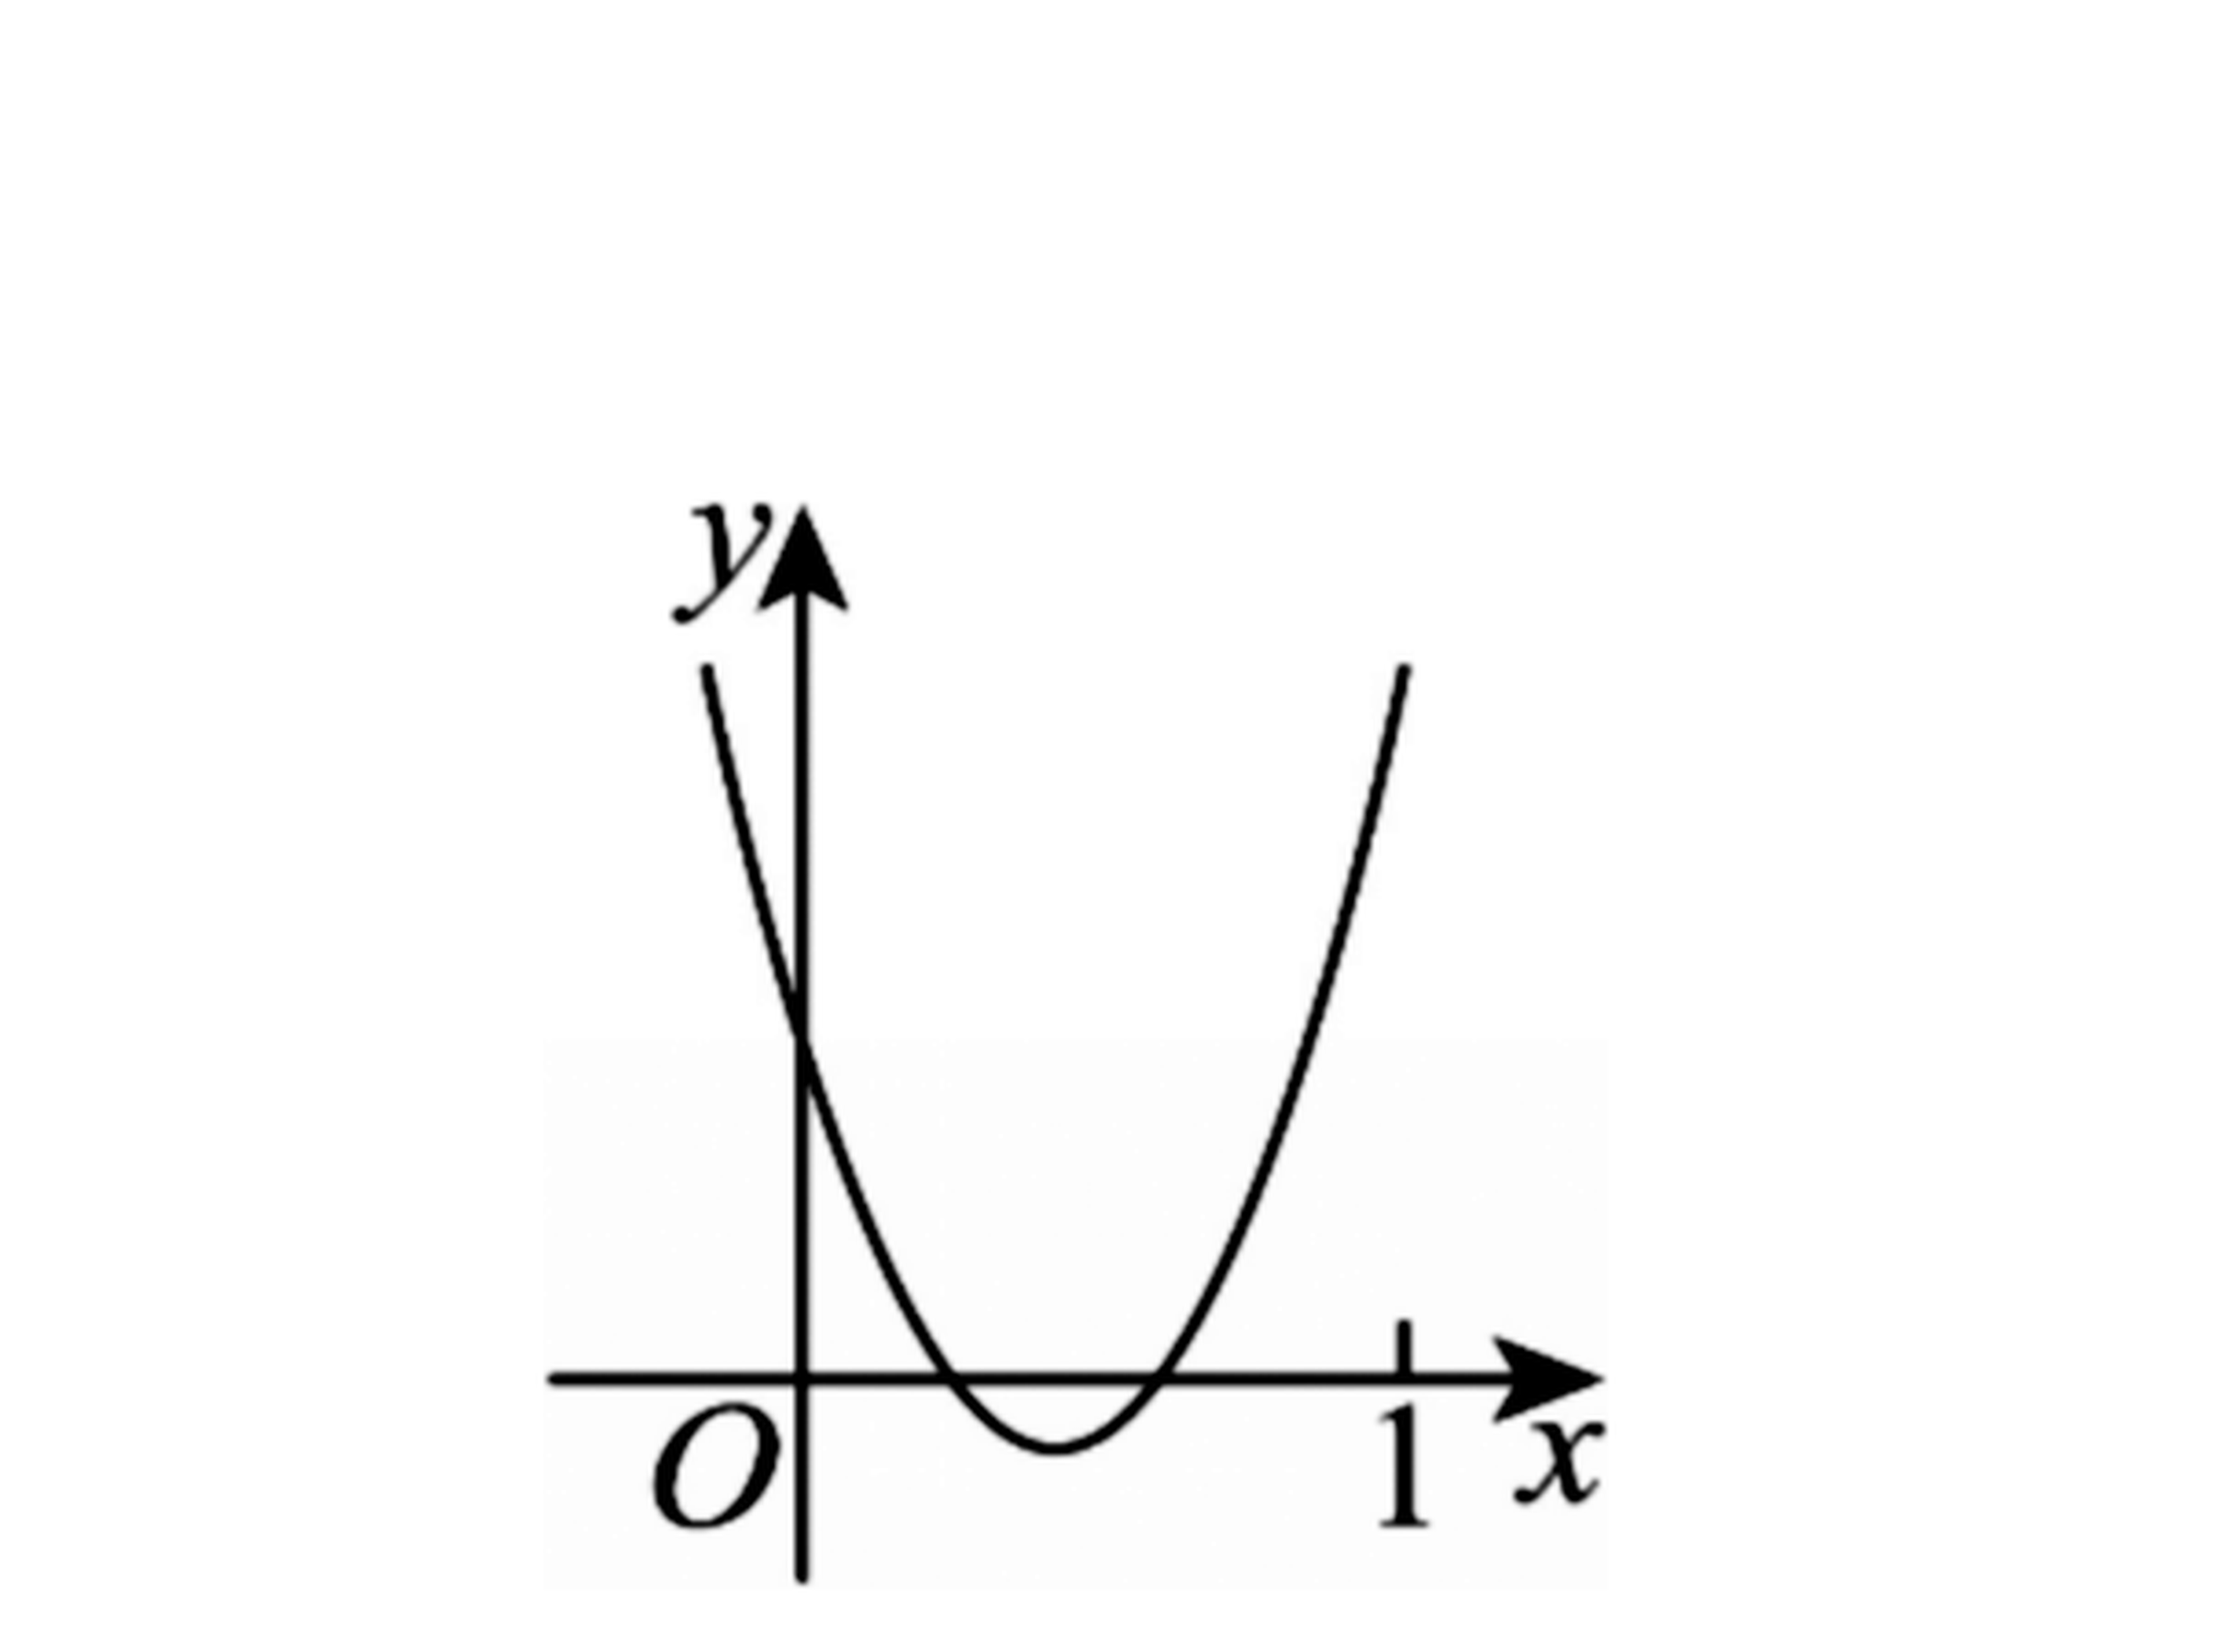
\includegraphics[width=0.32\textwidth]{figures/gao154_q15_stem.png}
\end{center}

\keepwithprev
\begin{center}
% 四幅指数函数图像选项取 05 页上半，按原卷 2×2 排布合并为一张，去粉色水印、去色、4× LANCZOS 放大；三版都出
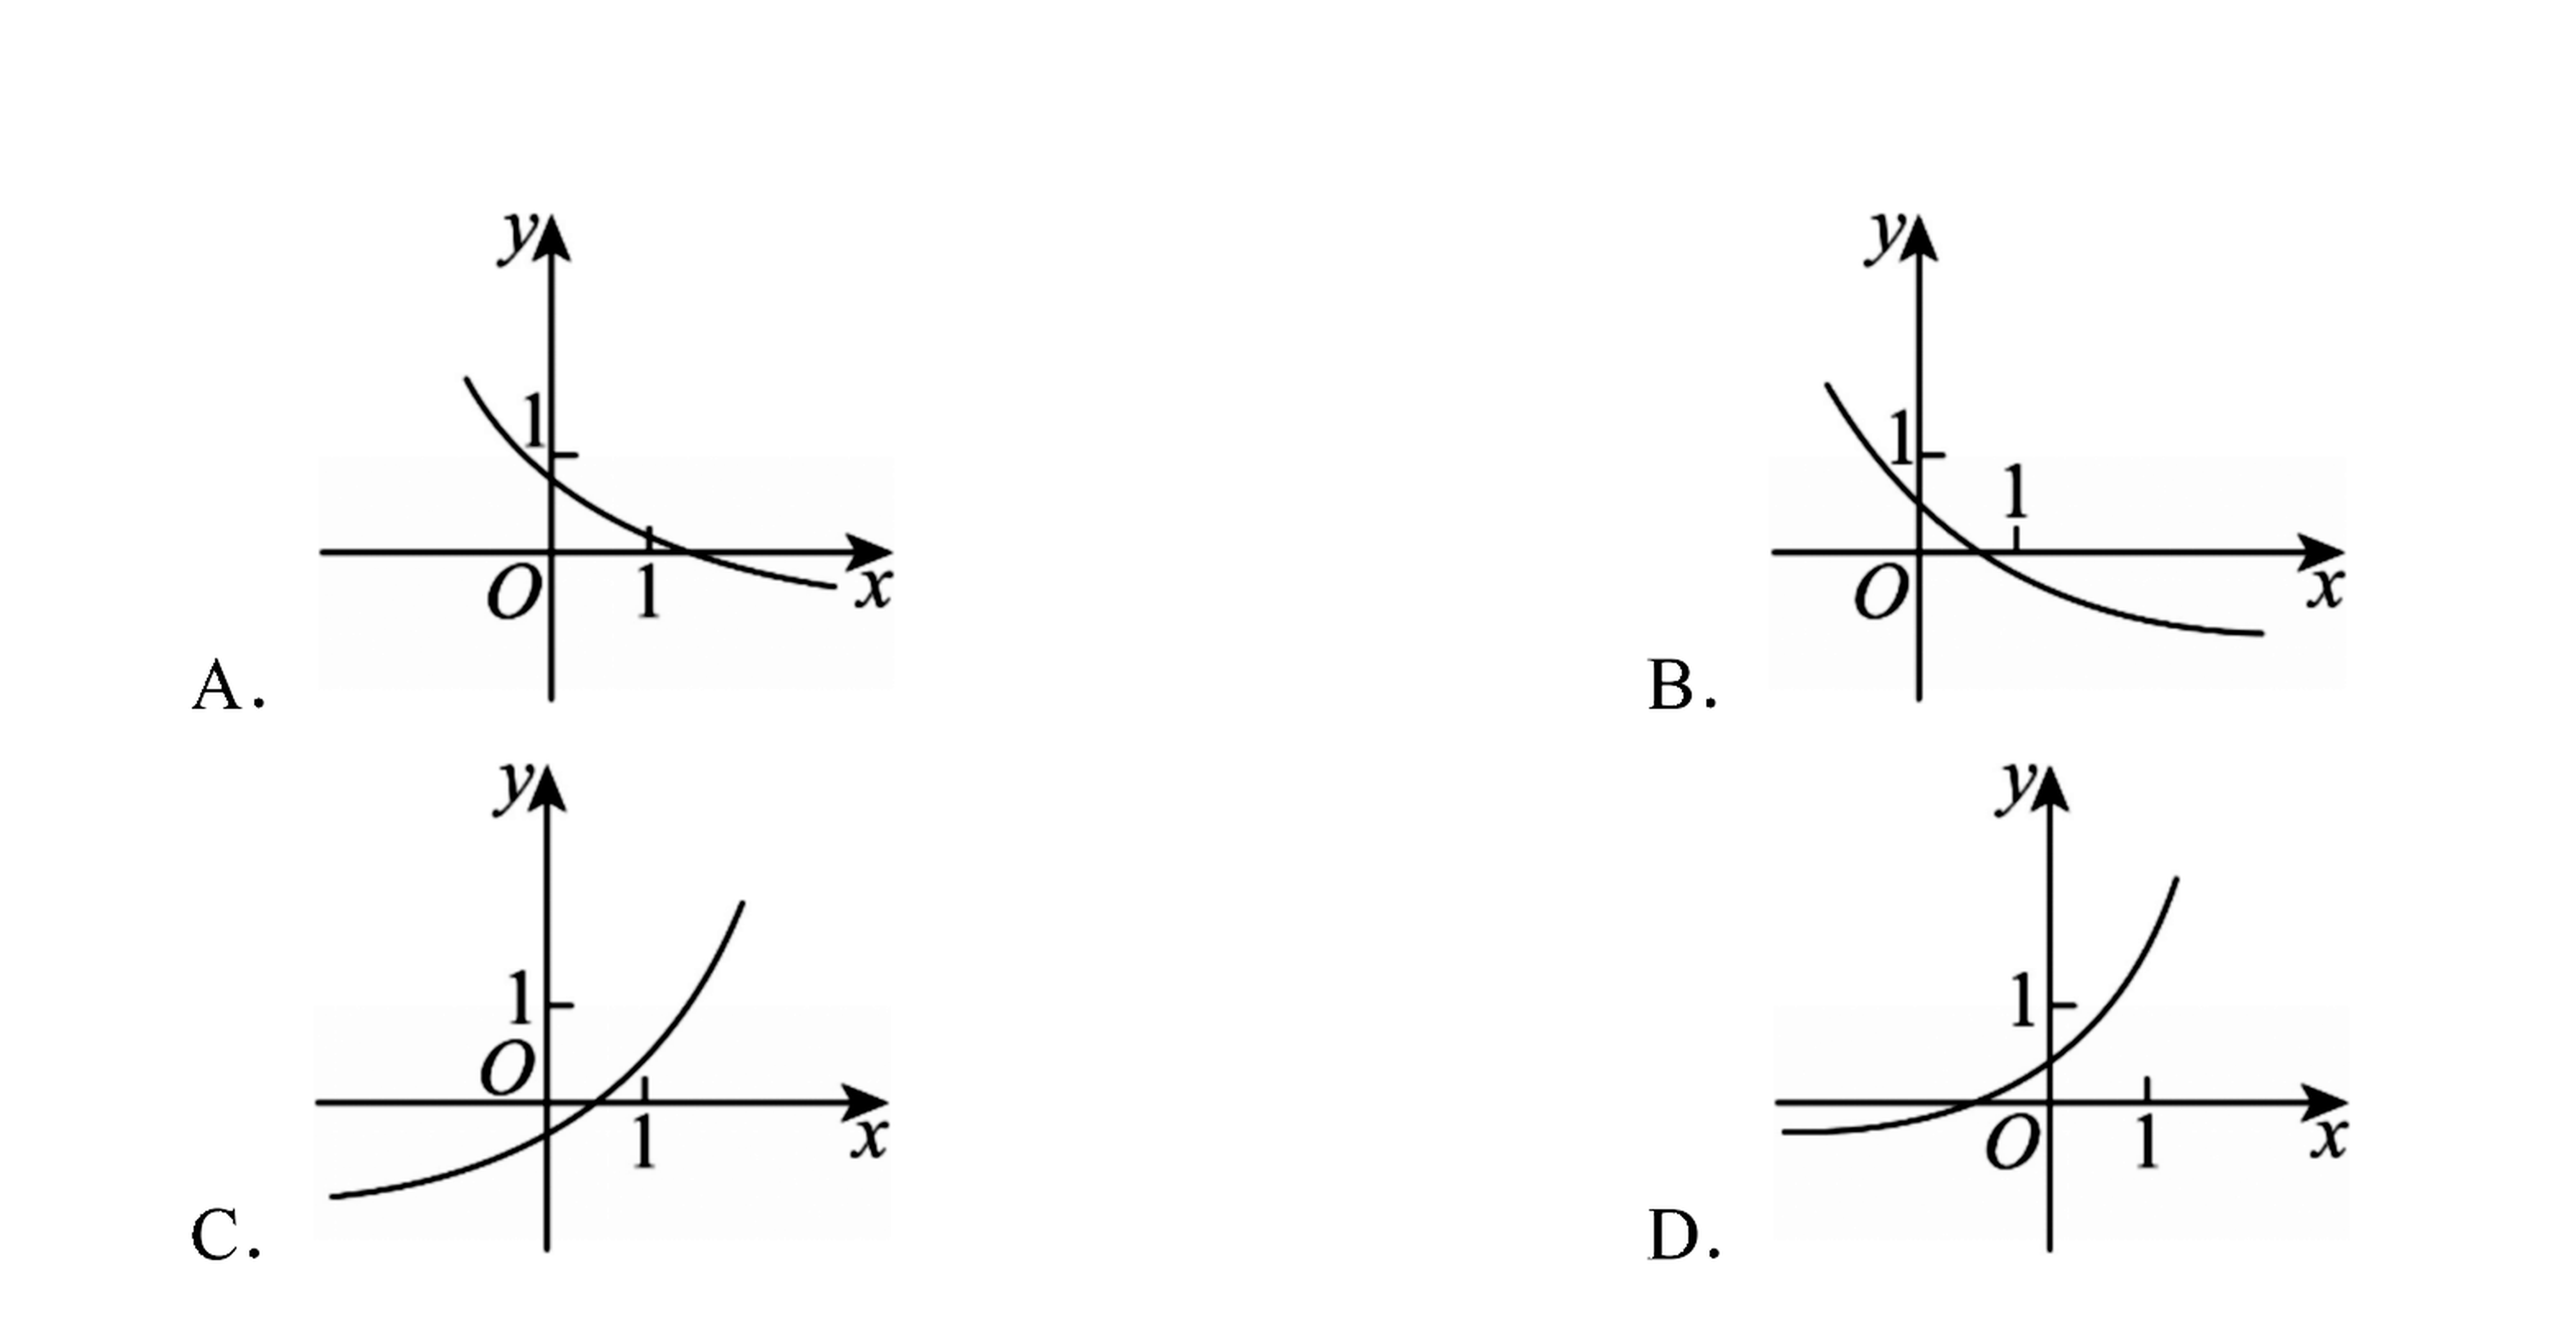
\includegraphics[width=0.80\textwidth]{figures/gao154_q15_opts.png}
\end{center}

\ifanswer
\solbegin
\step{由题意得 $0<a<b<1$，所以 $g(x)=a^x-b$ 在定义域 $\R$ 上严格减.}
\step{$g(0)=a^0-b=1-b>0$，$g(1)=a^1-b=a-b<0$，故 B 符合题意.}
\step{故选 $B$.}
\solend
\fi

% === Q16 === 高斯取整；解析 13 行，故选 C
\item 设 $[a]$ 表示不超过 $a$ 的最大整数，如 $[1.2]=1$，$[-3.2]=-4$，若 $x$、$y$、$z$ 为正实数，则 $\left[\dfrac{y+z}{x}\right]+\left[\dfrac{z+x}{y}\right]+\left[\dfrac{x+y}{z}\right]$ 的最小值为\mbox{（\quad）}

\keepwithprev
A. 2\qquad\qquad B. 3\qquad\qquad C. 4\qquad\qquad D. 6

\ifanswer
\solbegin
\step{若 $x$、$y$、$z$ 为正实数，}
\step{结合基本不等式得 $\dfrac{y+z}{x}+\dfrac{z+x}{y}+\dfrac{x+y}{z}=\dfrac yx+\dfrac xy+\dfrac zx+\dfrac xz+\dfrac zy+\dfrac yz$}
\step{$\geqslant2\sqrt{\dfrac yx\cdot\dfrac xy}+2\sqrt{\dfrac zx\cdot\dfrac xz}+2\sqrt{\dfrac zy\cdot\dfrac yz}=6$，当且仅当 $x=y=z$ 时取等号，}
\step{即 $\dfrac{y+z}{x}$，$\dfrac{z+x}{y}$，$\dfrac{x+y}{z}$ 中至少有一个不小于 2，不妨设 $\dfrac{y+z}{x}\geqslant\dfrac{z+x}{y}\geqslant\dfrac{x+y}{z}$，}
\step{$[a]$ 表示不超过 $a$ 的最大整数和 $\dfrac{y+z}{x}$，$\dfrac{z+x}{y}$，$\dfrac{x+y}{z}$ 中至少有一个不小于 2，}% 原卷此行把两句连写，照录未改（见 ⑤ 3）
\step{得 $\left[\dfrac{y+z}{x}\right]\geqslant2$，所以 $\left[\dfrac{y+z}{x}\right]+\left[\dfrac{z+x}{y}\right]+\left[\dfrac{x+y}{z}\right]\geqslant2$，}
\step{假设 $\left[\dfrac{y+z}{x}\right]+\left[\dfrac{z+x}{y}\right]+\left[\dfrac{x+y}{z}\right]$ 的最小值为 2，$\left[\dfrac{y+z}{x}\right]=2$，$\left[\dfrac{z+x}{y}\right]+\left[\dfrac{x+y}{z}\right]=0$，}
\step{所以 $2\leqslant\dfrac{y+z}{x}<3$，$0<\dfrac{z+x}{y}<1$，$0<\dfrac{x+y}{z}<1$，所以 $2<\dfrac{y+z}{x}+\dfrac{z+x}{y}+\dfrac{x+y}{z}<5$，}
\step{与 $\dfrac{y+z}{x}+\dfrac{z+x}{y}+\dfrac{x+y}{z}\geqslant6$ 矛盾，假设不成立，A 错误；}
\step{假设 $\left[\dfrac{y+z}{x}\right]+\left[\dfrac{z+x}{y}\right]+\left[\dfrac{x+y}{z}\right]$ 的最小值为 3，}
\step{则 $\left[\dfrac{y+z}{x}\right]=2$，$\left[\dfrac{z+x}{y}\right]=1$，$\left[\dfrac{x+y}{z}\right]=0$ 或 $\left[\dfrac{y+z}{x}\right]=3$，$\left[\dfrac{z+x}{y}\right]=\left[\dfrac{x+y}{z}\right]=0$，}
\step{同理可得 $3<\dfrac{y+z}{x}+\dfrac{z+x}{y}+\dfrac{x+y}{z}<6$，显然不成立，B 错误；}
\step{假设 $\left[\dfrac{y+z}{x}\right]+\left[\dfrac{z+x}{y}\right]+\left[\dfrac{x+y}{z}\right]$ 的最小值为 4，易得 $4<\dfrac{y+z}{x}+\dfrac{z+x}{y}+\dfrac{x+y}{z}<7$，}
\step{若取 $x=100$，$y=103$，$z=104$，则 $\left[\dfrac{y+z}{x}\right]=2$，$\left[\dfrac{z+x}{y}\right]=1$，$\left[\dfrac{x+y}{z}\right]=1$，}
\step{即 $\left[\dfrac{y+z}{x}\right]+\left[\dfrac{z+x}{y}\right]+\left[\dfrac{x+y}{z}\right]=4$，假设成立，C 正确，D 错误.}
\step{故选 $C$.}
\solend
\fi

\end{enumerate}

\bigsec{三、解答题}

\begin{enumerate}
\setcounter{enumi}{16}

% === Q17 === $B\subset A$ 单线照录；cases 块；解析 5 行
\item 设集合 $A=\{x\mid x^2+2x-3<0\}$，集合 $B=\{x\mid\lvert x+a\rvert<1\}$.

(1) 若 $a=3$，求 $A\cup B$；

(2) 设命题 $p:x\in A$，命题 $q:x\in B$，若 $p$ 是 $q$ 成立的必要不充分条件，求实数 $a$ 的取值范围.

\ifanswer
\solbegin
\step{(1) $A=(-3,1)$，}
\step{当 $a=3$ 时，$\lvert x+3\rvert<1$，解得 $-4<x<-2$，所以 $B=(-4,-2)$，}
\step{所以 $A\cup B=(-4,1)$.}
\step{(2) 因为 $p$ 是 $q$ 成立的必要不充分条件，所以 $B\subset A$.}
\step{因为 $A=(-3,1)$，$B=(-a-1,-a+1)$，所以 $\begin{cases}-a-1\geqslant-3\\-a+1<1\end{cases}$ 或 $\begin{cases}-a-1>-3\\-a+1\leqslant1\end{cases}$，解得 $0\leqslant a\leqslant2$.}
\solend
\fi

% === Q18 === 判别式 \Delta 两处照录；解析 9 行
\item 已知关于 $x$ 的一元二次方程 $x^2-mx+4m^2-3=0$ 的两个实根分别为 $x_1,x_2$.

(1) 若 $x_1,x_2$ 满足 $x_1+x_2=x_1x_2$，求实数 $m$ 的值；

(2) 求 $x_1^2+x_2^2$ 的最小值.

\ifanswer
\solbegin
\step{(1) 由韦达定理 $x_1+x_2=m$，$x_1x_2=4m^2-3$，}
\step{$\Delta=m^2-4(4m^2-3)=-15m^2+12\geqslant0$，即 $m^2\leqslant\dfrac45$.}
\step{由 $x_1+x_2=x_1x_2$ 得 $m=4m^2-3$，即 $4m^2-m-3=0$，}
\step{解得 $m=1$ 或 $m=-\dfrac34$.}
\step{$m=1$ 时 $m^2=1>\dfrac45$，$\Delta<0$，舍去；}
\step{$m=-\dfrac34$ 时 $m^2=\dfrac9{16}<\dfrac45$，符合，故 $m=-\dfrac34$.}
\step{(2) $x_1^2+x_2^2=(x_1+x_2)^2-2x_1x_2=m^2-2(4m^2-3)=-7m^2+6$，}
\step{函数 $y=-7m^2+6$ 开口向下，对称轴为 $m=0$，}% 原卷此处称求「最小值」，实为闭区间 $m^2\le\frac45$ 上的最小值，照录未改（见 ⑤ 4）
\step{故 $y_{\min}=-7\cdot\dfrac45+6=-\dfrac{28}{5}+\dfrac{30}{5}=\dfrac25$.}
\solend
\fi

% === Q19 === 全称命题；cases 块；解析 9 行
\item 设命题 $p$：对任意 $x\in\R$，不等式 $2mx^2+2mx+1>0$ 恒成立，$q:m\in\{m\mid\log_2(m-1)<1\}$.

(1) 若 $p$ 为真命题，求实数 $m$ 的取值范围；

(2) 若命题 $p$、$q$ 有且只有一个是真命题，求实数 $m$ 的取值范围.

\ifanswer
\solbegin
\step{(1) 由 $p$ 为真命题，得 $\forall x\in\R$，不等式 $2mx^2+2mx+1>0$ 恒成立，}
\step{当 $m=0$ 时，$1>0$ 恒成立；}
\step{当 $m\ne0$ 时，$\begin{cases}2m>0\\\Delta=4m^2-8m<0\end{cases}$，解得 $0<m<2$；}
\step{综上，$0\leqslant m<2$，即 $m$ 的取值范围是 $[0,2)$；}
\step{(2) 若 $q$ 为真，则有 $\log_2(m-1)<1$，得 $0<m-1<2$，解得 $1<m<3$，}
\step{因此命题 $q:m\in\{m\mid1<m<3\}$，由 (1) 得命题 $p:\{m\mid0\leqslant m<2\}$，}
\step{而命题 $p$、$q$ 有且只有一个是真命题，}
\step{当 $p$ 真 $q$ 假时，$\begin{cases}0\leqslant m<2\\m\leqslant1\text{ 或 }m\geqslant3\end{cases}$，解得 $0\leqslant m\leqslant1$，}
\step{当 $p$ 假 $q$ 真时，$\begin{cases}m<0\text{ 或 }m\geqslant2\\1<m<3\end{cases}$，解得 $2\leqslant m<3$，}
\step{故实数 $m$ 的取值范围是 $\{m\mid0\leqslant m\leqslant1\text{ 或 }2\leqslant m<3\}$.}
\solend
\fi

% === Q20 === Labubu 成本题；解析 10 行
\item Labubu 公司拟在 2027 年初推出智能机器人系列玩偶（单位：套）. 根据以往经验，其中一条生产线每月生产 $x$ 套玩具的成本 $P$ 由两部分费用（单位：元）构成：

(i) 固定成本（与生产玩具套数 $x$ 无关），总计 160000 元；

(ii) 每生产 $x$ 套需另投入的生产成本 $c(x)$ 元，其中 $c(x)=10x+\dfrac1{100}x^2$.

(1) 假设该生产线每月生产出的玩具能全部售出，问：该生产线每月生产玩具多少套时，可使得平均每套所需成本费用最少？此时每套玩具的成本费用是多少？

(2) 假设该生产线每月生产出的玩具能全部售出，但随着 $x$ 的增大，每月生产所需的直接总成本在急剧增加，因此售价也需随着 $x$ 的增大而适当增加. 设每套玩具的售价为 $q(x)$ 元，$q(x)=a+\dfrac xb$（$a,b\in\R$）. 若当月产量为 10000 套时利润最大，此时每套售价为 150 元，试求 $a,b$ 的值.（利润=销售收入$-$成本费用）

\ifanswer
\solbegin
\step{(1) 每月总成本 $P=160000+10x+\dfrac1{100}x^2$，}
\step{平均每套成本为 $\dfrac Px=\dfrac{160000}{x}+10+\dfrac x{100}\geqslant10+2\sqrt{\dfrac{160000}{x}\cdot\dfrac x{100}}=90$.}
\step{等号成立当且仅当 $\dfrac{160000}{x}=\dfrac x{100}$ 时，即 $x=4000$ 时取等号，}
\step{所以每月生产 4000 套时平均每套成本最少，此时每套成本为 90 元.}
\step{(2) 利润 $W(x)=x\cdot q(x)-P=\left(\dfrac1b-\dfrac1{100}\right)x^2+(a-10)x-160000$.}
\step{要在 $x=10000$ 处取得最大值，需 $\dfrac1b-\dfrac1{100}<0$，且对称轴为 $x=10000$，}
\step{故 $-\dfrac{a-10}{2\left(\frac1b-\frac1{100}\right)}=10000$，即 $a-10=-20000\left(\dfrac1b-\dfrac1{100}\right)$.}
\step{又 $q(10000)=a+\dfrac{10000}{b}=150$.}
\step{令 $t=\dfrac1b$，则 $a=150-10000t$，}
\step{代入上式 $140-10000t=-20000t+200$，解得 $t=\dfrac3{500}$，即 $b=\dfrac{500}{3}$；}
\step{再由 $a=150-10000\times\dfrac3{500}=150-60=90$，所以 $a=90$，$b=\dfrac{500}{3}$.}
\solend
\fi

% === Q21 === $A^+$／$A^-$ 新定义；$A\subseteq$ 带下划线照录、\varnothing；解析 16 行
\item 设集合 $A$ 为非空数集，定义 $A^+=\{x\mid x=a+b,a,b\in A\}$，$A^-=\{x\mid x=\lvert a-b\rvert,a,b\in A\}$.

(1) 若集合 $A=\{-1,1\}$，写出集合 $A^+$ 及 $A^-$；

(2) 若集合 $A=\{x_1,x_2,x_3,x_4\}$，$x_1<x_2<x_3<x_4$，且 $A^-=A$，求证：$x_1+x_4=x_2+x_3$；

(3) 若集合 $A\subseteq\{x\mid0\leqslant x\leqslant2020,x\in\N\}$，且 $A^+\cap A^-=\varnothing$，求集合 $A$ 元素的个数的最大值.

\ifanswer
\solbegin
\step{(1) 由 $A=\{-1,1\}$，得 $A^+=\{-2,0,2\}$，$A^-=\{0,2\}$；}
\step{(2) 由于集合 $A=\{x_1,x_2,x_3,x_4\}$，$x_1<x_2<x_3<x_4$，且 $A^-=A$，}
\step{所以 $A^-$ 中也只包含四个元素，即 $A^-=\{0,x_2-x_1,x_3-x_1,x_4-x_1\}$，}
\step{剩下的 $x_3-x_2=x_4-x_3=x_2-x_1$，所以 $x_1+x_4=x_2+x_3$；}
\step{(3) 设 $A=\{a_1,a_2,\cdots,a_k\}$ 满足题意，其中 $a_1<a_2<\cdots<a_k$，}
\step{则 $2a_1<a_1+a_2<a_1+a_3<\cdots<a_1+a_k<a_2+a_k<a_3+a_k<\cdots<a_{k-1}+a_k<2a_k$，所以 $\lvert A^+\rvert\geqslant2k-1$，}
\step{且 $a_1-a_1<a_2-a_1<a_3-a_1<\cdots<a_k-a_1$，所以 $\lvert A^-\rvert\geqslant k$，}
\step{因为 $A^+\cap A^-=\varnothing$，所以 $\lvert A^+\cup A^-\rvert=\lvert A^+\rvert+\lvert A^-\rvert\geqslant3k-1$，}
\step{$A^+\cup A^-$ 中最小的元素为 0，最大的元素为 $2a_k$，所以 $\lvert A^+\cup A^-\rvert\leqslant2a_k+1$，}
\step{所以 $3k-1\leqslant2a_k+1\leqslant4041$（$k\in\N^*$），所以 $k\leqslant1347$，}
\step{实际上当 $A=\{674,675,676,\cdots,2020\}$ 时满足题意，证明如下：}
\step{设 $A=\{m,m+1,m+2,\cdots,2020\}$，$m\in\N$，}
\step{则 $A^+=\{2m,2m+1,2m+2,\cdots,4040\}$，$A^-=\{0,1,2,\cdots,2020-m\}$，}
\step{由题意得 $2020-m<2m$，即 $m>673\dfrac13$，}
\step{故 $m$ 的最小值为 674，于是当 $m=674$ 时，$A$ 中元素最多，}
\step{即 $A=\{674,675,676,\cdots,2020\}$ 时满足题意，}
\step{综上所述，集合 $A$ 中元素的个数的最大值是 1347.}
\solend
\fi

\end{enumerate}

\bigsec{附加题}

\begin{enumerate}

% === 附加题 1 === 另起编号 1；「n 元集和集」弯引号；解析 6 行
\item 设集合 $A=\{a_1,a_2,a_3,a_4\}$，$C=\{2,3,4,6\}$，新定义：集合 $A$ 中所有含 $n$ 个元素的子集中 $n$ 个元素之和的不同值组成的集合为“$n$ 元集和集”. 若 $A$ 的“3 元集和集”为 $C$，则集合 $A=$\blankline[4.4em].

\ifanswer
\solbegin
\step{集合 $A$ 的 3 元子集共有 4 个：$\{a_1,a_2,a_3\}$，$\{a_1,a_2,a_4\}$，$\{a_1,a_3,a_4\}$，$\{a_2,a_3,a_4\}$，}
\step{集合 $C=\{a_1+a_2+a_3,a_1+a_2+a_4,a_1+a_3+a_4,a_2+a_3+a_4\}$，}
\step{不妨令 $a_1<a_2<a_3<a_4$，}
\step{则 $a_1+a_2+a_3<a_1+a_2+a_4<a_1+a_3+a_4<a_2+a_3+a_4$，}
\step{而 $C=\{2,3,4,6\}$，因此 $\begin{cases}a_1+a_2+a_3=2\\a_1+a_2+a_4=3\\a_1+a_3+a_4=4\\a_2+a_3+a_4=6\end{cases}$，相加化简得 $a_1+a_2+a_3+a_4=5$，}
\step{解得 $a_1=-1$，$a_2=1$，$a_3=2$，$a_4=3$，所以 $A=\{-1,1,2,3\}$.}
\solend
\fi

% === 附加题 2 === 解析配图（仅答案版出）；四选项；解析 15 行，故选 A
\item 已知函数 $f(x)=\log_p x+q$，其中 $p>0$ 且 $p\ne1$，曲线 $y=f(x)$ 经过 $P(1,2)$、$Q(2,3)$ 两点. 设 $g(x)=f(x)\cdot[f(x)-2]$，若 $\lvert g(a)\rvert=\lvert g(b)\rvert=\lvert g(c)\rvert=\lvert g(d)\rvert$，且 $a<b<c<d$，则 $ad(b+c)$ 的取值范围为\mbox{（\quad）}

\keepwithprev
A. $\left(\dfrac14,\dfrac5{16}\right)$\qquad B. $\left(\dfrac18,\dfrac5{16}\right)$\qquad C. $\left(\dfrac14,\dfrac25\right)$\qquad D. $\left(\dfrac18,\dfrac25\right)$

\ifanswer
\solbegin
\step{函数 $f(x)=\log_p x+q$，且曲线 $y=f(x)$ 经过点 $P(1,2)$ 和 $Q(2,3)$，}
\step{所以 $\begin{cases}f(1)=q=2\\f(2)=\log_p2+q=3\end{cases}$，解得 $p=2$，$q=2$，$f(x)=\log_2 x+2$.}
\step{不妨设 $\lvert g(x)\rvert=k$，令 $\log_2 x=m$，则 $f(x)\cdot[f(x)-2]=m(m+2)=m^2+2m$，}
\step{画出函数 $y=\lvert m^2+2m\rvert$ 的图象，如图所示，}
\begin{center}
% $y=|m(m+2)|$ 图像取 11 页右上，去粉色水印、去色、4× LANCZOS 放大；仅答案版出
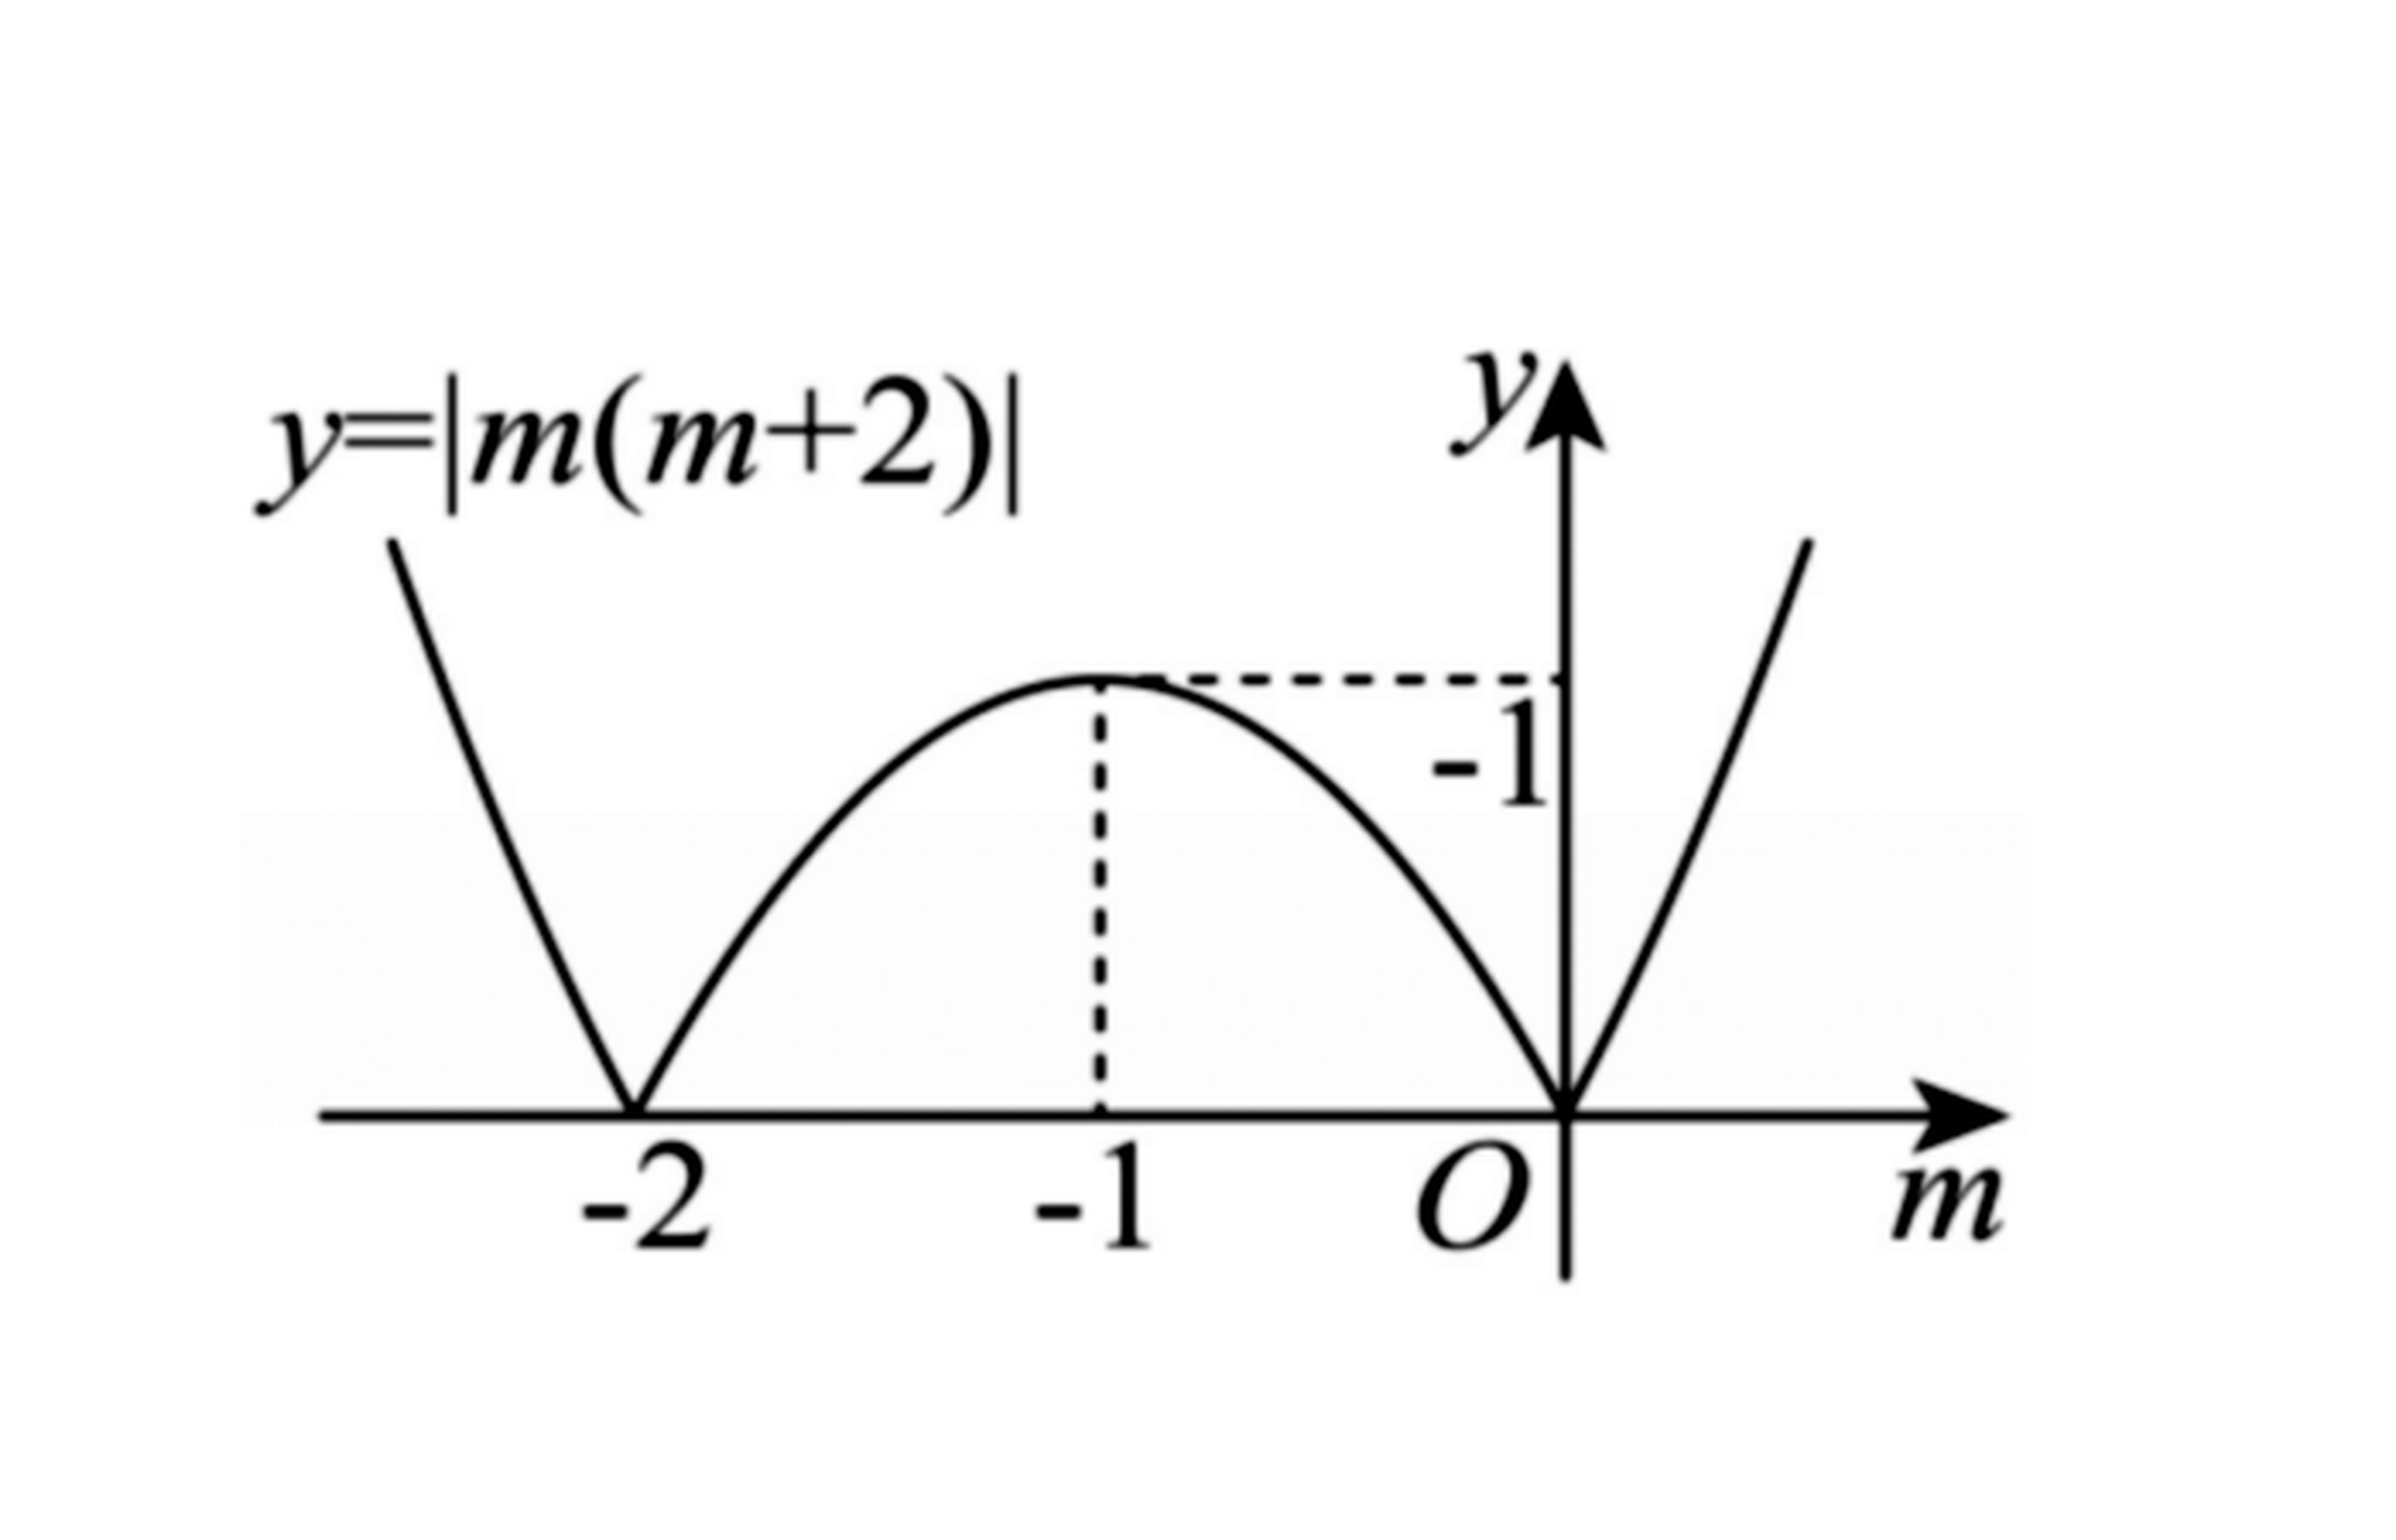
\includegraphics[width=0.46\textwidth]{figures/gao154_fujia2.png}
\end{center}
\step{由图像得 $k\in(0,1)$，}
\step{所以方程 $m^2+2m=k$ 和 $m^2+2m=-k$ 各有两个不同的根，}
\step{其中方程 $m^2+2m-k=0$ 的两根为 $m=-1\pm\sqrt{1+k}$，}
\step{方程 $m^2+2m+k=0$ 的两根为 $m=-1\pm\sqrt{1-k}$，}
\step{所以 $m_1=-1-\sqrt{1+k}$，$m_2=-1-\sqrt{1-k}$，$m_3=-1+\sqrt{1-k}$，$m_4=-1+\sqrt{1+k}$，且 $m_1<m_2<m_3<m_4$，}
\step{由 $m=\log_2 x$，则 $x=2^m$，}
\step{所以 $a=2^{-1-\sqrt{1+k}}$，$b=2^{-1-\sqrt{1-k}}$，$c=2^{-1+\sqrt{1-k}}$，$d=2^{-1+\sqrt{1+k}}$，}
\step{所以 $ad=2^{-1-\sqrt{1+k}}\times2^{-1+\sqrt{1+k}}=2^{(-1-\sqrt{1+k})+(-1+\sqrt{1+k})}=2^{-2}=\dfrac14$，}
\step{$b+c=2^{-1-\sqrt{1-k}}+2^{-1+\sqrt{1-k}}=\dfrac{2^{-\sqrt{1-k}}+2^{\sqrt{1-k}}}{2}$，}
\step{令 $s=\sqrt{1-k}$，其中 $s\in(0,1)$，则 $b+c=\dfrac12\left(2^{-s}+2^s\right)$，}
\step{设函数 $y=2^s+\dfrac1{2^s}$，令 $r=2^s\in(1,2)$，所以 $y=r+\dfrac1r$ 在 $(1,2)$ 上严格增，}
\step{所以函数 $y=2^s+\dfrac1{2^s}$ 在 $(0,1)$ 上严格增，所以 $y=2^s+\dfrac1{2^s}\in\left(2,\dfrac52\right)$，}
\step{所以 $b+c=\dfrac{2^{-s}+2^s}{2}\in\left(1,\dfrac54\right)$，$ad(b+c)=\dfrac{b+c}{4}\in\left(\dfrac14,\dfrac5{16}\right)$，}
\step{所以 $ad(b+c)$ 的取值范围是 $\left(\dfrac14,\dfrac5{16}\right)$，故选 $A$.}
\solend
\fi

\end{enumerate}

\end{document}
"
%
% ① 原始材料：微信公众号"魔都数学加油站"文章，连载"27学年高一154"，原文标题
% "27学年高一154——2026-2027年上海市徐汇中学高一上期中"；
% 原文链接：https://mp.weixin.qq.com/s/Qs2T7Zwsug-KKFE2wefDUg 。
% 正文为 12 张 PNG 页（01/03/04/05/07/11/12 为 2560×3620，
% 02/06/08/09/10 为 4762×6735，同一篇各页分辨率混排，逐页按各自分辨率裁图核对）。
% 体例：讲评版——一、填空题 3—12（10 题）、二、选择题 13—16（4 题）、
% 三、解答题 17—21（5 题）、附加题 1—2（2 题，原卷**另起编号**"1." "2."，
% 不与正题连号，同 高一a 成例），共 21 题；全卷每题均印【解析】
% （逐题核实，见 ② ②）。题目、答案、解析均据原图转录；卷面粉红色水印
% "魔都数学加油站"及公众号页脚未录入。
% 全卷插图清单（逐页通读 12 页确认）：3 组——
%   · Q15 题干配图（$f(x)=(x-a)(x-b)$ 抛物线，04 页右下：x/y 轴、O、1、
%     开口向上两零点均在 (0,1) 内），三版都出，裁 figures/gao154_q15_stem.png；
%   · Q15 四幅图像选项（05 页上半 2×2 排布，A/B/C/D 四幅指数函数图像，
%     合并成一张，照 高一136 Q13/Q22 成例），三版都出，
%     裁 figures/gao154_q15_opts.png；
%   · 附加题第 2 题解析配图（$y=\lvert m(m+2)\rvert$ 图像，11 页右上：
%     W 形折线、$-2$、$-1$、O、虚线 $y=1$ 与 $m=-1$），仅答案版出，
%     裁 figures/gao154_fujia2.png；
%   3 图均取自原卷截图，去粉色水印、去色、4× LANCZOS 放大；Q15 题干图
%   左侧题干残字"的图"已裁白。其余各页逐页确认无其它题目配图、无表格；
%   12 页下半仅水印、无正文。
%
% 卷首标题：原卷印作"2026-2027 年徐汇中学高一上期中"，年份区间按全稿惯例排 en dash；
% 原卷卷面未印副标题，本稿按同期中卷知识模块口径补出"集合与常用逻辑用语、不等式、函数"。
%
% ② 与原卷的排版差异：
%   ① 原文从第 3 题起，本稿保留原题号；共 21 题四节，正题到 21，附加题另起编号
%      1—2（\bigsec{附加题} 后 \begin{enumerate} 不 \setcounter，同 高一a 成例）；
%   ② 全 21 题均印【解析】、用 \solbegin…\solend，无只印【答案】或答案印括号内的题；
%      四道正题选择题答案在解析末句"故选 C／A／B／C"（Q13—Q16）、附加题第 2 题
%      答案在解析末句"故选 A"，括号 \mbox{（\quad）} 留空、不另提 \ans{}；
%      答案版【答案】/【解析】标记数 = 21 = 全卷题数；
%   ③ 原卷卷面未印副标题，本稿按知识模块口径补出；
%   ④ 原卷填空横线按全稿惯例排 \blankline[4.4em]；选择题括号排 \mbox{（\quad）}、
%      四道正题选择题与附加题第 2 题的选项段前按惯例各加 \keepwithprev
%      （Q15 与附加题 2 的选项段是整块图，\keepwithprev 后接 \begin{center}）；
%      解答题不留作答区、不加 \anspace（原卷为讲评版）；
%   ⑤ 数集黑板粗体：Q4"$x,y\in R$"、Q9"$x\in\R$"、Q13 无、
%      Q15"定义域 $\R$"、Q19"$\forall x\in\R$"、Q21"$x\in\N$"与"$k\in\N^*$"、
%      Q20"$a,b\in\R$"、附加题 2 无——原卷印斜体或正体粗体 R/N/N*，
%      按全稿惯例归一 \R／\N／\N^*；绝对值排 \lvert…\rvert
%      （Q5、Q9、Q12、Q13、Q16、Q21、附加题 2），集合描述竖线排 \mid
%      （Q5、Q17、Q19、Q21），不等号按全稿惯例排 \leqslant／\geqslant；
%      空集 \varnothing（Q21 题干 (3)）；
%   ⑥ 子集符号逐处照录、不得统一：Q6 题干印"$\{1,2\}\subset M\subseteq\{1,2,3,4,5\}$"
%      （前单线 ⊂、后带下划线 ⊆，同句两形并用），解析亦两形并用；
%      Q17 解析 (2)"$B\subset A$"印单线 ⊂；Q21 题干 (3)"$A\subseteq\{x\mid\cdots\}$"
%      印带下划线 ⊆——逐处放大核，分别 \subset／\subseteq，照录未统一（见 ④）；
%   ⑦ 判别式 Δ/△：Q18 解析 (1)"$\Delta=m^2-4(4m^2-3)$"与 Q19 解析 (1)
%      "$\Delta=4m^2-8m<0$"两处均印等腰偏高粗三角、照录 \Delta；本卷无扁等边
%      细线 \triangle 用例（见 ④）；
%   ⑧ 中文弯引号照录：Q4"设 $x$、$y\in\R$. 若 $x+y>2$，则 $x>1$ 或 $y>1$"、
%      附加题 1"$n$ 元集和集"与"3 元集和集"；注释里一律 ASCII 引号；
%      数学式内 CJK 用 \text{}（Q5 解集描述"或"、Q19 集合描述的"或"）；
%   ⑨ "图像／图象"逐处放大核：Q15 题干与解析印"图象"（象，无亻）、
%      Q16 无、附加题 2 解析印"图象"与"图像"（"画出函数…的图象"、
%      "由图像得"——两形并用，逐处照录未统一）；Q13/Q14 无数集图像字样；
%      半角逗号在数学组之间是全稿惯例、非笔误，逐处照录（Q3、Q10、Q16、
%      Q18、Q20、Q21 的 $x_1,x_2$ 之类）；行末西文句点 ASCII `.`；
%      行中全角逗号／顿号照录（Q6"3，4，5"、Q20"（单位：元）"、
%      附加题 1"$a_1,a_2,a_3,a_4$"）；
%   ⑩ 复杂式照录别简化：Q3 $a^{\frac{12}{7}}\cdot\left(\frac17\right)^{\frac17}
%      \cdot\sqrt[7]{a^4}$ 与 $7^{-\frac17}a^{\frac{16}{7}}$、Q7 $x^{-m}$、
%      Q8 $\frac{b-2a+2}{2a}$、Q11 $\frac{9+4\sqrt2}{6}$、Q12 $506\frac29$ 与
%      $506\frac49$、Q16 高斯取整 $[a]$、Q20 $c(x)=10x+\frac1{100}x^2$ 与
%      $q(x)=a+\frac xb$、Q21 $A^+$／$A^-$ 与 $|A^+|\geqslant2k-1$、
%      附加题 2 $m=-1\pm\sqrt{1+k}$ 与 $ad(b+c)$；
%      \left…\right 不得拆到不同 $…$ 组（Q5 $\left\{x\mid\cdots\right\}$、
%      Q20 $\left(\frac1b-\frac1{100}\right)$、附加题 2 $\left(\frac14,\frac5{16}\right)$）；
%      cases 块一律 \begin{cases}…\end{cases}；
%   ⑪ 一条 \step = 原卷解析的一个印刷行，cases 块整体算一个印刷行；别并折行、
%      别拆行。Q11 九行、Q12 六行、Q16 十六行、Q20 十一行、Q21 十七行、
%      附加题 2 十八行均按印刷行逐条断，不丢行；
%   ⑫ 配图：Q15 题干小图（三版都出）放 \item 内题干之后 \begin{center}，
%      Q15 四幅选项图（三版都出）放 \keepwithprev 之后的 \begin{center}，
%      Q15 用 \needvspace 守卫把"题干＋两图"整块推走（守卫放 \item 之前，
%      见 高一145 Q14/Q20 与 高一136 Q13 成例）；附加题 2 解析配图（仅答案版出）
%      放 \ifanswer 内 \solbegin…\solend 的 \step 之间（高一73 第 16 题成例）；
%   ⑬ 原卷解析内无红色"法一／法二"之类小标题，故本卷无 \stepm；红色水印
%      "魔都数学加油站"不录入；
%   ⑭ 跨页续印按题合并：见 ⑥；
%
% ③ 行数复核：一条 \step = 原卷解析的一个印刷行，cases 块作一个印刷行计。
%   逐题数（主会话逐页核对定稿）：Q3：1；Q4：1；Q5：3；Q6：4；Q7：3；
%   Q8：1；Q9：5；Q10：4；Q11：9；Q12：6；Q13：5；Q14：4；Q15：3；
%   Q16：16；Q17：5；Q18：9；Q19：10；Q20：11；Q21：17；
%   附加题 1：6；附加题 2：18。
%   合计 141 条 \step（本卷无 \stepm），与原卷逐题印刷行相等。全卷 21 题
%   均设 \solbegin…\solend，答案版【答案】/【解析】标记数 = 21 = 全卷题数。
%
% ④ 判别式／子集符号结论（逐处放大原图照录、不得统一，主会话像素级复核）：
%   判别式：Q18 解析 (1)"$\Delta=m^2-4(4m^2-3)=-15m^2+12\geqslant0$"、
%      Q19 解析 (1)"$\Delta=4m^2-8m<0$"共 2 处，逐处放大确认印等腰偏高
%      粗三角（高>宽、右斜边粗），照录 \Delta；本卷无扁等边细线 \triangle
%      用例，无几何三角形符号。
%   子集：Q6 题干"$\{1,2\}\subset M\subseteq\{1,2,3,4,5\}$"前 ⊂ 单线、
%      后 ⊆ 带下划线（/tmp/gao154/z/zoom/q6_subset.png），解析两处同样两形
%      并用，分别照录 \subset／\subseteq；Q17 解析 (2)"$B\subset A$"单线
%      照录 \subset；Q21 题干 (3)"$A\subseteq\{x\mid\cdots\}$"带下划线
%      照录 \subseteq。本卷 ⊂ 与 ⊆ 混用逐处照录、不得统一。
%      空集 \varnothing（Q21 题干 (3)）、数集 \R／\N／\N^* 归一见 ② ⑤。
%
% ⑤ 存疑照录（放大原图确认，照录未改、正文对应处另有 % 注）：
%   1. Q7 题干印 $f(x)=(3m-1)x^{-m}$，解析首句却写"幂函数 $f(x)=x^\alpha$
%      的系数必须为 1"（用 $\alpha$ 作指数记号），随后 $f(2)=2^\alpha=8$
%      得 $\alpha=3$、$f(x)=x^3$——题干指数 $-m$ 与解析 $\alpha$ 记法不同，
%      系原卷记号前后不一，逐处照录未统一（放大 01/02 页确认）。
%   2. Q11 解析"因为 $u>0,v>0$，由基本不等式得 $\frac{4v}{u}+\frac{2u}{v}
%      \geqslant2\sqrt{\frac{4v}{u}\cdot\frac{2u}{v}}=4\sqrt2$"与
%      "所以 $\frac4u+\frac1v=\frac16\left(\frac4u+\frac1v\right)(2u+v)$"
%      照录，未把 $u,v$ 化简回 $x,y$。
%   3. Q16 解析把"$[a]$ 表示不超过 $a$ 的最大整数"与"和至少有一个不小于 2"
%      连写在同一行（原卷如此），照录未改；末行"假设成立，C 正确，D 错误"照录。
%   4. Q18 解析 (2)"函数 $y=-7m^2+6$ 开口向下，对称轴为 $m=0$"却称求
%      "$y_{\min}$"（实为在 $m^2\leqslant\frac45$ 闭区间上的最小值），
%      照录未改。
%   5. Q20 题干"$q(x)=a+\frac xb$（$a,b\in\R$）"与解析
%      "$W(x)=\left(\frac1b-\frac1{100}\right)x^2+(a-10)x-160000$"照录；
%      末行解得 $a=90,b=\frac{500}{3}$ 照录未化简。
%   6. Q21 题干 (3)"$A\subseteq\{x\mid0\leqslant x\leqslant2020,x\in\N\}$"
%      与解析"$3k-1\leqslant2a_k+1\leqslant4041$（$k\in\N^*$）"照录；
%      末行"集合 $A$ 中元素的个数的最大值是 1347"照录。
%   7. 附加题 1 解析"相加化简得 $a_1+a_2+a_3+a_4=5$"照录；
%      附加题 2 解析"由图像得 $k\in(0,1)$"与"由图像得"／"的图象"两形
%      并用逐处照录（见 ② ⑨）；末行"$ad(b+c)$ 的取值范围是
%      $\left(\frac14,\frac5{16}\right)$，故选 A"照录。
%   全卷除此 7 类外未发现其它笔误／自相矛盾处；21 题均印【解析】、
%   无只印【答案】或答案印括号内的题（见 ② ②）。
%
% ⑥ 跨页续印按题合并说明（逐页核实定稿）：Q3—Q5 题干＋解析在 01 页
%   （Q5 解析末 2 行续 01 页下半）；Q6、Q7 题干＋解析在 01 页下半
%   （Q7 解析余 2 行续 02 页顶）；Q8、Q9 题干＋解析在 02 页上半
%   （Q9 解析余 3 行续 02 页下半）；Q10 题干＋解析在 02 页下半；
%   Q11 题干＋解析前 6 行在 03 页上半、余 3 行续 03 页下半；
%   Q12 题干＋解析前 5 行在 03 页下半、末行续 04 页顶；"二、选择题"
%   标题与 Q13 题干＋选项＋解析在 04 页上半；Q14 题干＋选项＋解析、
%   Q15 题干＋题干配图在 04 页下半；Q15 四幅选项图＋解析、
%   Q16 题干＋选项＋解析首行在 05 页上半，Q16 解析余 12 行在
%   05 页下半—06 页上半；"三、解答题"标题与 Q17 题干＋两问＋解析
%   在 06 页下半；Q18 题干＋两问＋解析在 07 页上半—下半；
%   Q19 题干＋两问＋解析首行在 07 页下半，解析余 8 行在 08 页上半；
%   Q20 题干在 08 页下半，解析 (1) 4 行＋(2) 首 4 行在 08 页下半—09 页上半，
%   (2) 余 2 行在 09 页下半；Q21 题干＋三问＋解析 (1)(2) 4 行在
%   09 页下半—10 页上半，解析 (3) 余 12 行在 10 页上半—下半；
%   "附加题"标题与附加题 1 题干＋解析首 3 行在 10 页下半，
%   余 3 行续 11 页上半；附加题 2 题干＋选项＋解析前 3 行在 11 页上半，
%   解析配图＋余 12 行在 11 页下半—12 页上半，末行
%   "所以 $ad(b+c)$ 的取值范围是 $\left(\frac14,\frac5{16}\right)$，故选 A"
%   为全卷收尾（12 页下半仅水印、无正文）。
%   本稿按题连排，不丢行、不并折行；全卷末题为附加题第 2 题。
%
\documentclass[a4paper,11pt]{article}
\usepackage{common}

\begin{document}

\examtitlest[3]{2026--2027 年徐汇中学高一上期中}{集合与常用逻辑用语、不等式、函数}

\bigsec{一、填空题}

\begin{enumerate}
\setcounter{enumi}{2}

% === Q3 === 分数指数幂照录；解析 1 行
\item 已知 $a>0$，化简 $a^{\frac{12}{7}}\cdot\left(\dfrac17\right)^{\frac17}\cdot\sqrt[7]{a^4}=$\blankline[4.4em].

\ifanswer
\solbegin
\step{$a^{\frac{12}{7}}\cdot\left(\dfrac17\right)^{\frac17}\cdot\sqrt[7]{a^4}=a^{\frac{12}{7}}\cdot(7^{-1})^{\frac17}\cdot a^{\frac47}=7^{-\frac17}a^{\frac{16}{7}}$.}
\solend
\fi

% === Q4 === 反证法；中文弯引号照录；解析 1 行
\item 用反证法证明命题：“设 $x$、$y\in\R$. 若 $x+y>2$，则 $x>1$ 或 $y>1$”时，假设的内容应该是\blankline[4.4em].

\ifanswer
\solbegin
\step{由反证法得，假设的内容应该是 $x\leqslant1$ 且 $y\leqslant1$.}
\solend
\fi

% === Q5 === 分式不等式；cases 块；解析 3 行
\item 不等式 $\dfrac{2x+3}{x-1}\geqslant1$ 的解集为\blankline[4.4em].

\ifanswer
\solbegin
\step{$\dfrac{2x+3}{x-1}\geqslant1$，即 $\dfrac{2x+3}{x-1}-1\geqslant0$，$\dfrac{x+4}{x-1}\geqslant0$，}
\step{等价于 $\begin{cases}(x+4)(x-1)\geqslant0\\x-1\ne0\end{cases}$，解得 $x>1$ 或 $x\leqslant-4$，}
\step{故解集为 $\{x\mid x>1\text{ 或 }x\leqslant-4\}$.}
\solend
\fi

% === Q6 === ⊂ 与 ⊆ 并用照录；解析 4 行
\item 满足条件 $\{1,2\}\subset M\subseteq\{1,2,3,4,5\}$ 的集合 $M$ 的个数为\blankline[4.4em].

\ifanswer
\solbegin
\step{因为 $\{1,2\}\subset M\subseteq\{1,2,3,4,5\}$，所以集合 $M$ 必含有元素 1，2，}
\step{且至少含有元素 3，4，5 中的一个，}
\step{则集合 $M$ 的个数与集合 $\{3,4,5\}$ 的非空子集的个数一样，}
\step{所以集合 $M$ 的个数为 $2^3-1=7$.}
\solend
\fi

% === Q7 === 题干 $x^{-m}$、解析用 $x^\alpha$ 记法，原卷记号差异照录（见 ⑤ 1）；解析 3 行
\item 已知幂函数 $f(x)=(3m-1)x^{-m}$，且 $f(2)=8$，则 $f(m)=$\blankline[4.4em].

\ifanswer
\solbegin
\step{幂函数 $f(x)=x^\alpha$ 的系数必须为 1，所以 $3m-1=1$，得 $m=\dfrac23$.}
\step{又 $f(2)=2^\alpha=8=2^3$，故 $\alpha=3$，即 $f(x)=x^3$，}
\step{所以 $f(m)=f\left(\dfrac23\right)=\left(\dfrac23\right)^3=\dfrac8{27}$.}
\solend
\fi

% === Q8 === 换底公式；解析 1 行
\item 已知 $a=\lg2$，$b=\lg3$，用含 $a,b$ 的代数式表示 $\log_4 75=$\blankline[4.4em].

\ifanswer
\solbegin
\step{$\log_4 75=\dfrac{\lg\left(3\times\frac{10^2}{2^2}\right)}{\lg2^2}=\dfrac{\lg3+2-2\lg2}{2\lg2}=\dfrac{b-2a+2}{2a}$.}
\solend
\fi

% === Q9 === 三角不等式取等；解析 5 行
\item 设 $x\in\R$，则方程 $\lvert x-2\rvert+\lvert3x+1\rvert=\lvert2x+3\rvert$ 的解集是\blankline[4.4em].

\ifanswer
\solbegin
\step{由 $\lvert x-2\rvert=\lvert2-x\rvert$，故原方程可化为 $\lvert2-x\rvert+\lvert3x+1\rvert=\lvert2x+3\rvert$，}
\step{又 $(2-x)+(3x+1)=2x+3$，}
\step{由三角不等式 $\lvert2-x\rvert+\lvert3x+1\rvert\geqslant\lvert(2-x)+(3x+1)\rvert=\lvert2x+3\rvert$，}
\step{当且仅当 $(2-x)(3x+1)\geqslant0$ 等号成立，}
\step{解 $(2-x)(3x+1)\geqslant0$ 得 $-\dfrac13\leqslant x\leqslant2$，故原方程的解集为 $\left[-\dfrac13,2\right]$.}
\solend
\fi

% === Q10 === 韦达定理；cases 块；解析 4 行
\item 已知一元二次不等式 $x^2+bx+c>0$ 的解集为 $(-\infty,-1)\cup(2,+\infty)$，则一元二次不等式 $bx^2+cx-1<0$ 的解集是\blankline[4.4em].

\ifanswer
\solbegin
\step{因为 $x^2+bx+c>0$ 的解集为 $(-\infty,-1)\cup(2,+\infty)$，}
\step{所以方程 $x^2+bx+c=0$ 的两根为 $-1$ 和 2，则有 $\begin{cases}-b=-1+2\\c=-1\times2\end{cases}$，即 $\begin{cases}b=-1\\c=-2\end{cases}$，}
\step{则 $bx^2+cx-1<0$ 等价于 $-x^2-2x-1<0$，得 $x^2+2x+1>0$，得 $(x+1)^2>0$，}
\step{解得 $x\ne-1$，故不等式 $bx^2+cx-1<0$ 的解集为 $(-\infty,-1)\cup(-1,+\infty)$.}
\solend
\fi

% === Q11 === 换元 $u,v$；解析 9 行
\item 已知正数 $x,y$ 满足 $2x+y=1$，则 $\dfrac4{x+2}+\dfrac1{y+1}$ 的最小值为\blankline[4.4em].

\ifanswer
\solbegin
\step{令 $u=x+2$，$v=y+1$，则 $u>2$，$v>1$，}
\step{且 $2u+v=2(x+2)+(y+1)=2x+y+5=6$.}
\step{因为 $u>0$，$v>0$，由基本不等式得 $\dfrac{4v}{u}+\dfrac{2u}{v}\geqslant2\sqrt{\dfrac{4v}{u}\cdot\dfrac{2u}{v}}=4\sqrt2$，}
\step{所以 $\dfrac4u+\dfrac1v=\dfrac16\left(\dfrac4u+\dfrac1v\right)(2u+v)=\dfrac16\left(9+\dfrac{4v}{u}+\dfrac{2u}{v}\right)\geqslant\dfrac{9+4\sqrt2}{6}$，}
\step{当且仅当 $\dfrac{4v}{u}=\dfrac{2u}{v}$，即 $u=\sqrt2v$ 时等号成立，}
\step{与 $2u+v=6$ 联立得 $u=\dfrac{6\sqrt2}{2\sqrt2+1}$，$v=\dfrac6{2\sqrt2+1}$，}
\step{此时 $x=u-2=\dfrac{2\sqrt2-2}{2\sqrt2+1}>0$，$y=v-1=\dfrac{5-2\sqrt2}{2\sqrt2+1}>0$，且 $2x+y=1$，}
\step{满足题设，所以下界可以取得，}
\step{因此 $\dfrac4{x+2}+\dfrac1{y+1}$ 的最小值为 $\dfrac{9+4\sqrt2}{6}$.}
\solend
\fi

% === Q12 === 2025 个整数解；解析 6 行
\item 若关于 $x$ 的不等式 $\lvert x-2k\rvert+\lvert x-3k\rvert<4k$ 共有 2025 个整数解，则实数 $k$ 的取值范围为\blankline[4.4em].

\ifanswer
\solbegin
\step{显然 $k>0$，由 $\lvert x-2k\rvert+\lvert x-3k\rvert<4k$，得 $\dfrac12k<x<\dfrac92k$，}
\step{因为该不等式共有 2025 个整数解，所以 $2024<\dfrac{9k}{2}-\dfrac k2\leqslant2026$，}
\step{解得 $506<k\leqslant506.5$，}
\step{由 $\dfrac k2\in(253,253.25]$，得这 2025 个整数解只能为 254、255、256、$\cdots$、2278，}
\step{所以 $2278<\dfrac{9k}{2}\leqslant2279$，解得 $506\dfrac29<k\leqslant506\dfrac49$，结合 $506<k\leqslant506.5$，}
\step{得 $k$ 的取值范围是 $\left(506\dfrac29,506\dfrac49\right]$.}
\solend
\fi

\end{enumerate}

\bigsec{二、选择题}

\begin{enumerate}
\setcounter{enumi}{12}

% === Q13 === 四选项一行；解析 5 行，故选 C
\item 若 $a<b<0$，则下列不等式中不成立的是\mbox{（\quad）}

\keepwithprev
A. $a-b>a$\qquad B. $\dfrac1a>\dfrac1b$\qquad C. $a^3>b^3$\qquad D. $\lvert a\rvert>\lvert b\rvert$

\ifanswer
\solbegin
\step{A 选项，因为 $b<0$，所以 $-b>0$，不等式两边同加上 $a$ 得 $a-b>a$，故 A 正确；}
\step{B 选项，因为 $a<b<0$，所以 $ab>0$，不等式两边同除以 $ab$，则 $\dfrac1b<\dfrac1a<0$，故 B 正确；}
\step{C 选项，不妨设 $a=-2$，$b=-1$，则 $a^3=-8$，$b^3=-1$，故 $a^3<b^3$，故 C 错误；}
\step{D 选项，因为 $a<b<0$，所以 $-a>-b$，即 $\lvert a\rvert>\lvert b\rvert$，故 D 正确.}
\step{故选 $C$.}
\solend
\fi

% === Q14 === 选项两行两列；解析 4 行，故选 A
\item 设命题 $p:x^2-5x+4\ne0$，命题 $q:x\ne1$，则 $p$ 是 $q$ 的\mbox{（\quad）}条件

\keepwithprev
A. 充分不必要\qquad\qquad B. 必要不充分

C. 充要\qquad\qquad D. 既不充分也不必要

\ifanswer
\solbegin
\step{$p:x^2-5x+4\ne0\Leftrightarrow(x-1)(x-4)\ne0\Leftrightarrow x\ne1$ 且 $x\ne4$；$q:x\ne1$.}
\step{充分性：当 $x\ne1$ 且 $x\ne4$ 时，$x\ne1$，所以 $p\Rightarrow q$；}
\step{必要性：当 $x\ne1$ 时，若 $x=4$，此时 $p$ 不成立，即 $q\nRightarrow p$；}
\step{所以 $p$ 是 $q$ 的充分不必要条件，故选 $A$.}
\solend
\fi

% === Q15 === 题干配图（三版都出）+ 四幅图像选项（2×2 合并，三版都出）；守卫放 \item 之前；解析 3 行，故选 B
\needvspace{9cm}
\item 已知函数 $f(x)=(x-a)(x-b)$（$a<b$）的图象如图所示，则函数 $g(x)=a^x-b$ 的图象可能是\mbox{（\quad）}

\begin{center}
% 抛物线题干配图取 04 页右下，去粉色水印、去色、4× LANCZOS 放大；三版都出
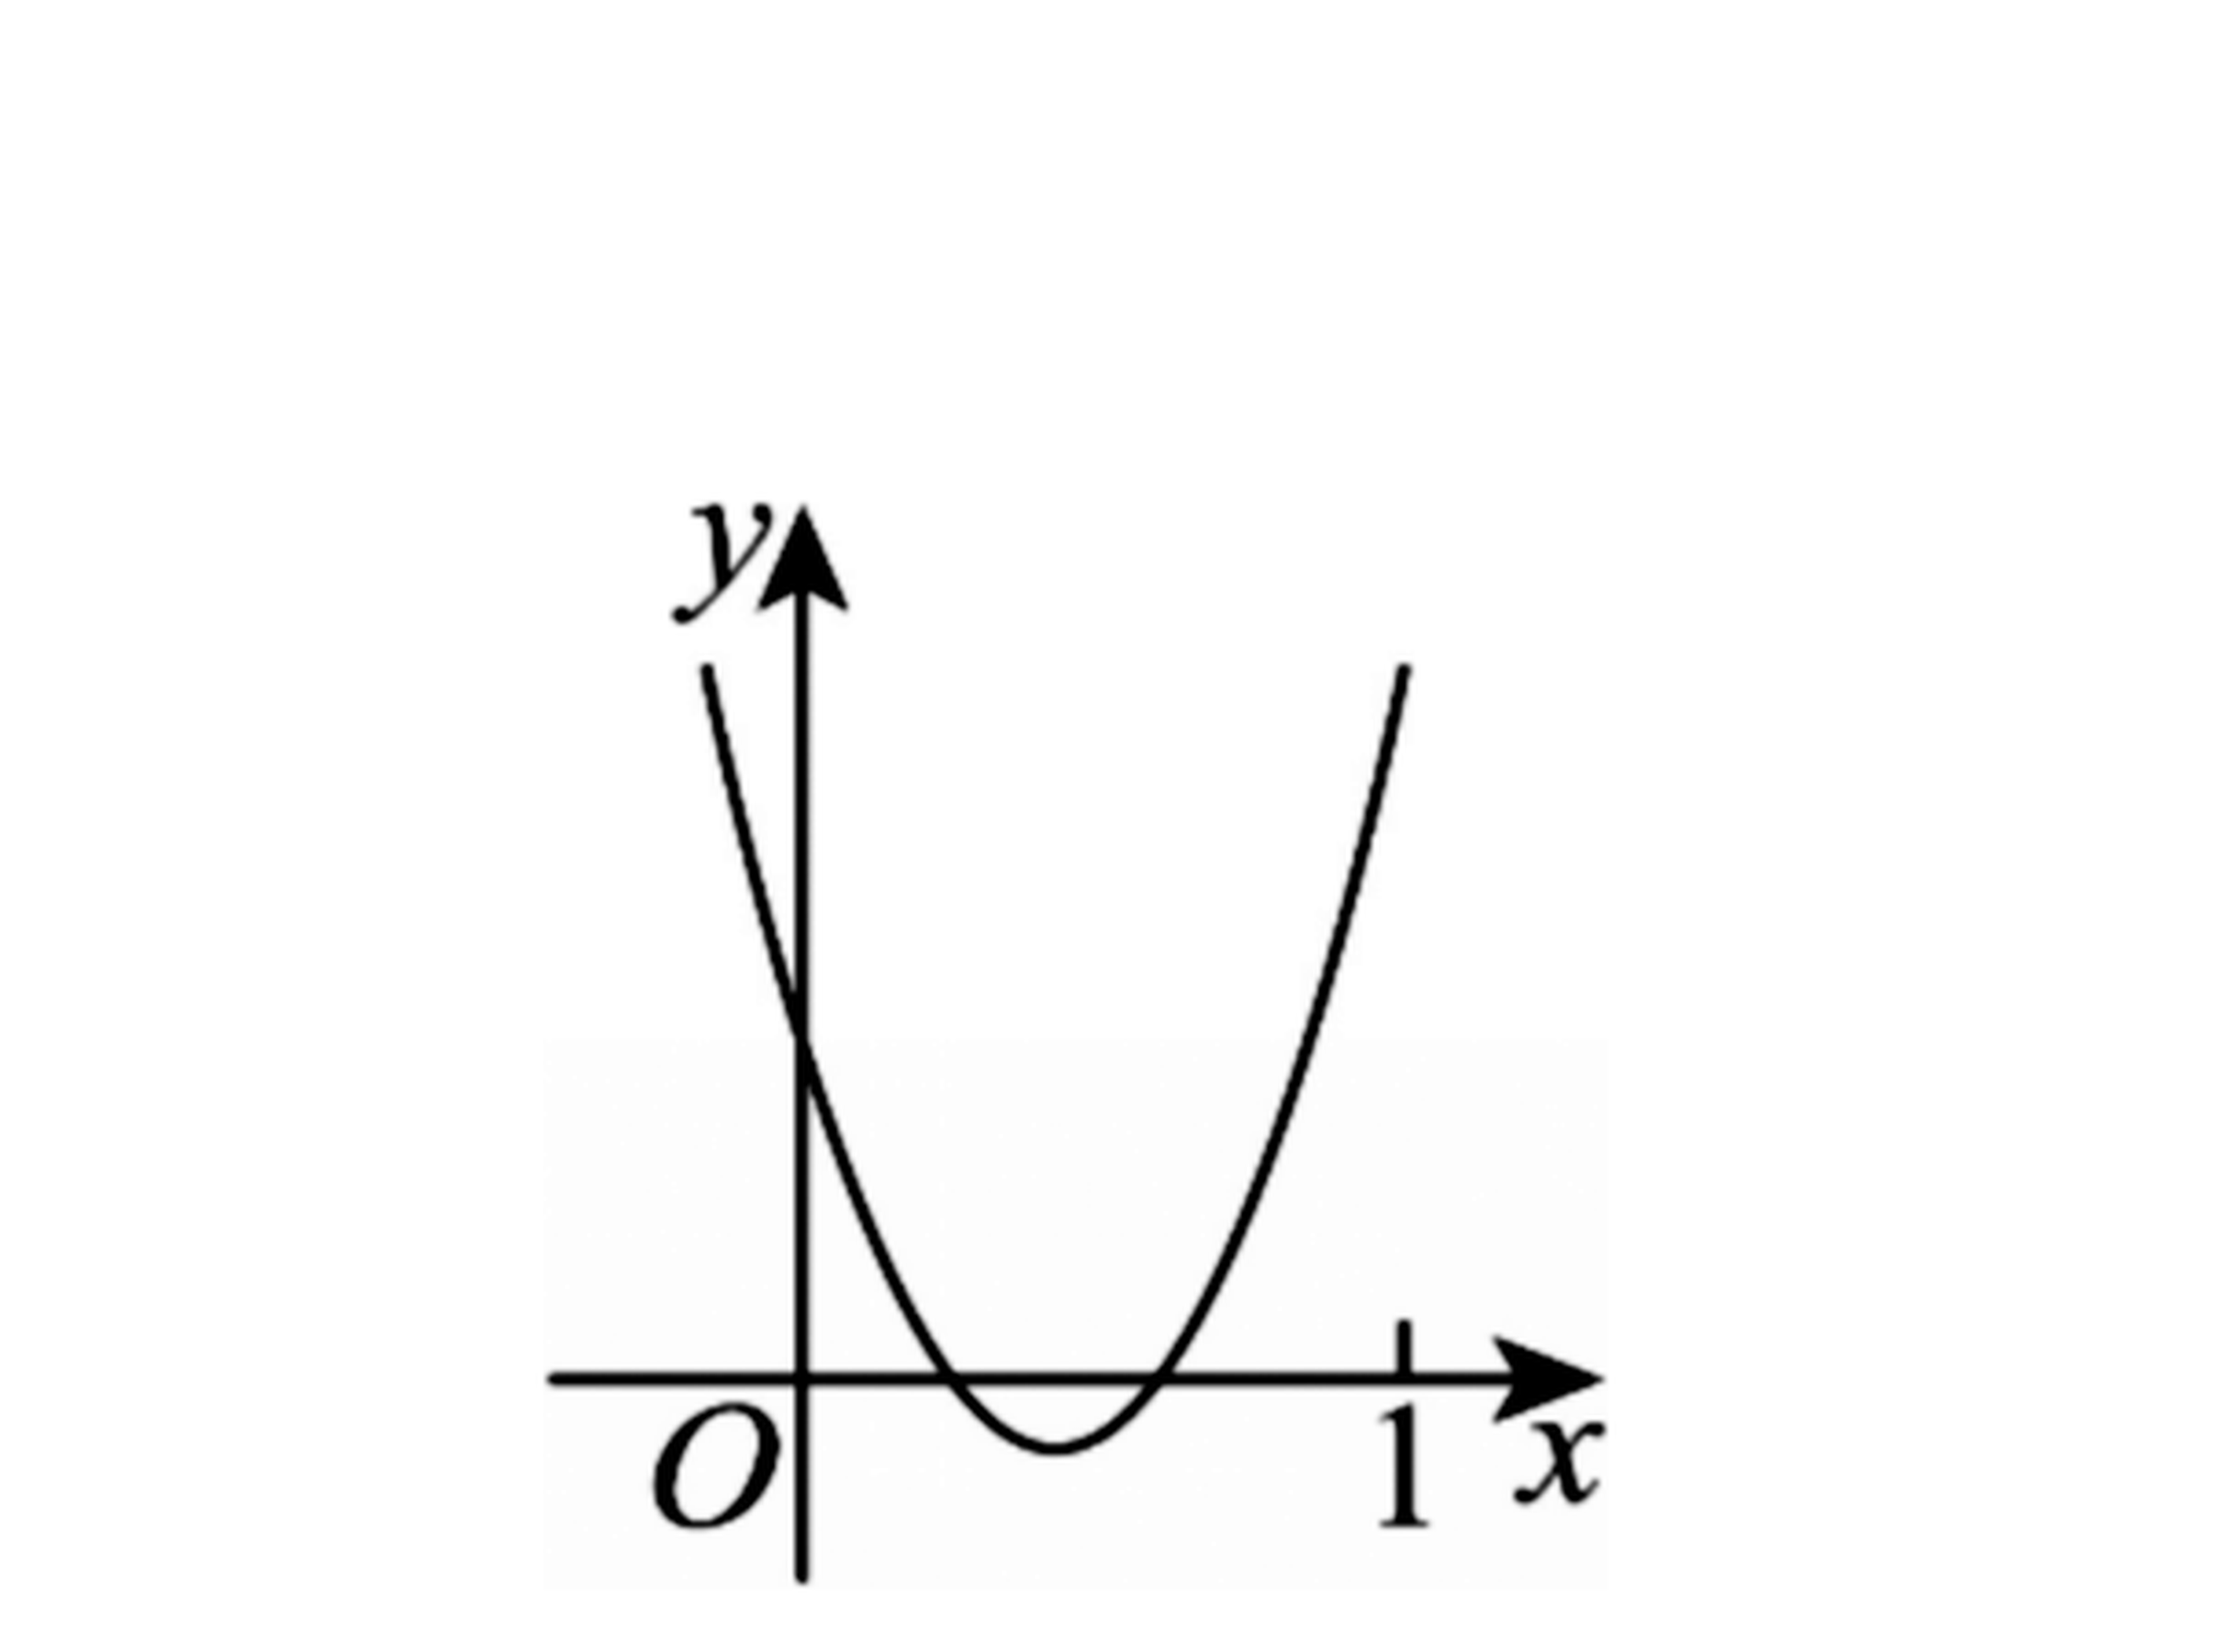
\includegraphics[width=0.32\textwidth]{figures/gao154_q15_stem.png}
\end{center}

\keepwithprev
\begin{center}
% 四幅指数函数图像选项取 05 页上半，按原卷 2×2 排布合并为一张，去粉色水印、去色、4× LANCZOS 放大；三版都出
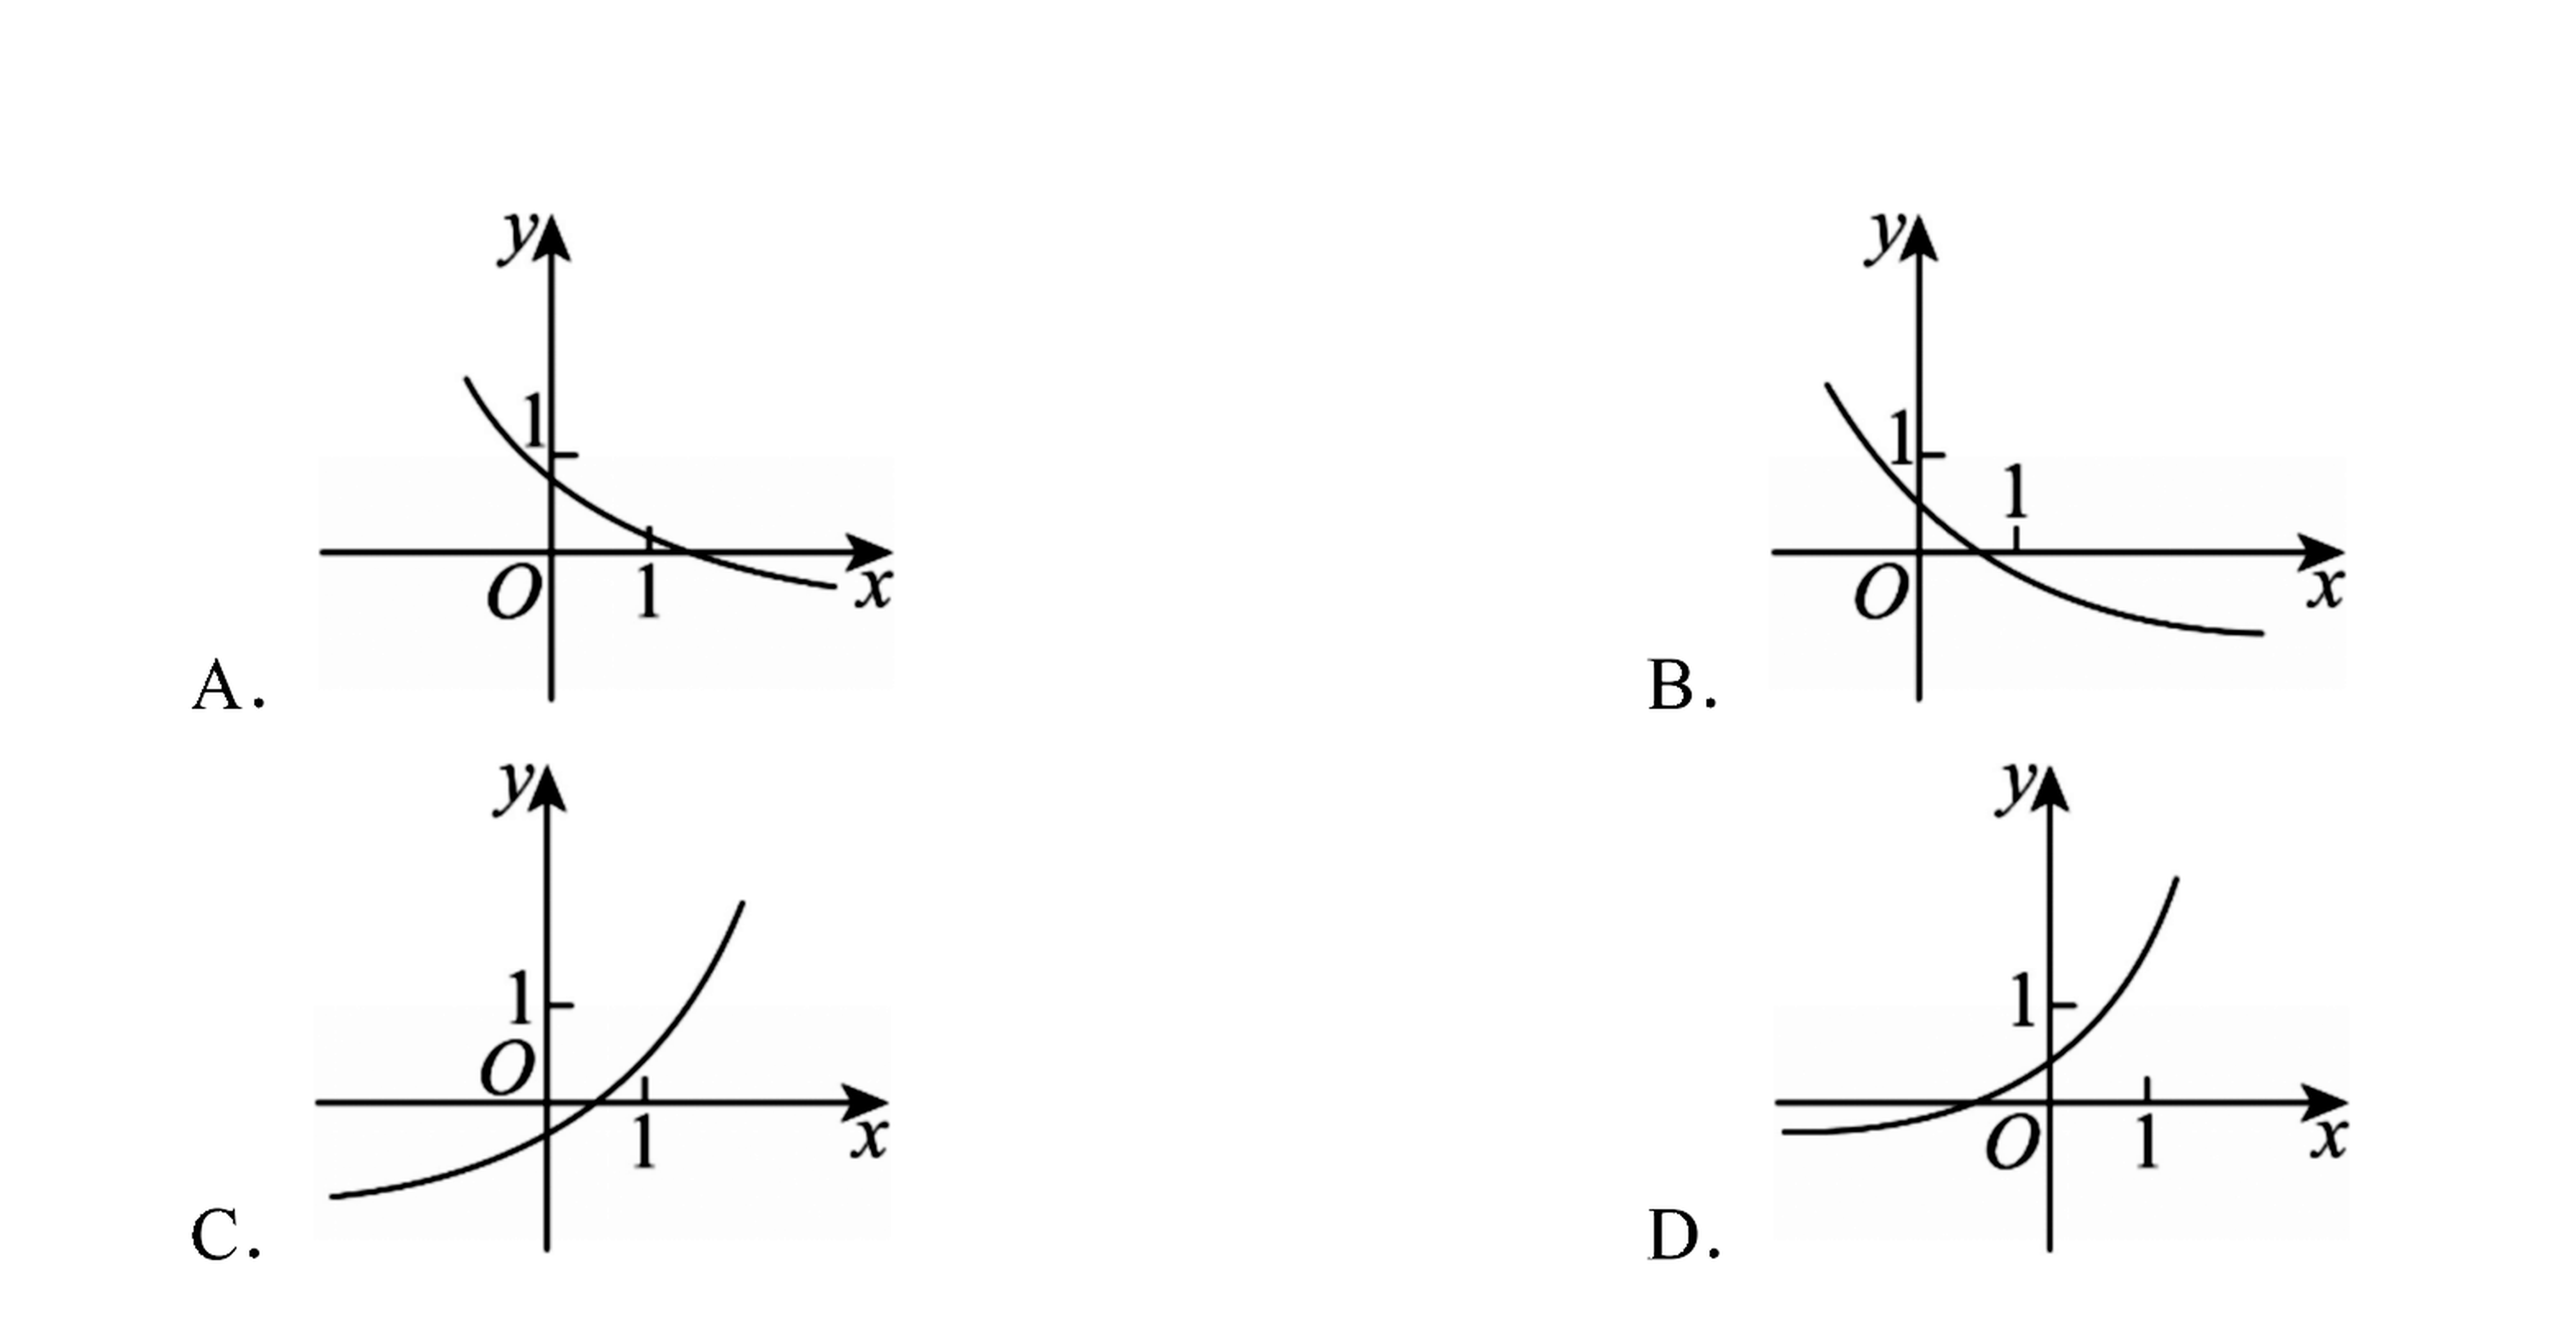
\includegraphics[width=0.80\textwidth]{figures/gao154_q15_opts.png}
\end{center}

\ifanswer
\solbegin
\step{由题意得 $0<a<b<1$，所以 $g(x)=a^x-b$ 在定义域 $\R$ 上严格减.}
\step{$g(0)=a^0-b=1-b>0$，$g(1)=a^1-b=a-b<0$，故 B 符合题意.}
\step{故选 $B$.}
\solend
\fi

% === Q16 === 高斯取整；解析 13 行，故选 C
\item 设 $[a]$ 表示不超过 $a$ 的最大整数，如 $[1.2]=1$，$[-3.2]=-4$，若 $x$、$y$、$z$ 为正实数，则 $\left[\dfrac{y+z}{x}\right]+\left[\dfrac{z+x}{y}\right]+\left[\dfrac{x+y}{z}\right]$ 的最小值为\mbox{（\quad）}

\keepwithprev
A. 2\qquad\qquad B. 3\qquad\qquad C. 4\qquad\qquad D. 6

\ifanswer
\solbegin
\step{若 $x$、$y$、$z$ 为正实数，}
\step{结合基本不等式得 $\dfrac{y+z}{x}+\dfrac{z+x}{y}+\dfrac{x+y}{z}=\dfrac yx+\dfrac xy+\dfrac zx+\dfrac xz+\dfrac zy+\dfrac yz$}
\step{$\geqslant2\sqrt{\dfrac yx\cdot\dfrac xy}+2\sqrt{\dfrac zx\cdot\dfrac xz}+2\sqrt{\dfrac zy\cdot\dfrac yz}=6$，当且仅当 $x=y=z$ 时取等号，}
\step{即 $\dfrac{y+z}{x}$，$\dfrac{z+x}{y}$，$\dfrac{x+y}{z}$ 中至少有一个不小于 2，不妨设 $\dfrac{y+z}{x}\geqslant\dfrac{z+x}{y}\geqslant\dfrac{x+y}{z}$，}
\step{$[a]$ 表示不超过 $a$ 的最大整数和 $\dfrac{y+z}{x}$，$\dfrac{z+x}{y}$，$\dfrac{x+y}{z}$ 中至少有一个不小于 2，}% 原卷此行把两句连写，照录未改（见 ⑤ 3）
\step{得 $\left[\dfrac{y+z}{x}\right]\geqslant2$，所以 $\left[\dfrac{y+z}{x}\right]+\left[\dfrac{z+x}{y}\right]+\left[\dfrac{x+y}{z}\right]\geqslant2$，}
\step{假设 $\left[\dfrac{y+z}{x}\right]+\left[\dfrac{z+x}{y}\right]+\left[\dfrac{x+y}{z}\right]$ 的最小值为 2，$\left[\dfrac{y+z}{x}\right]=2$，$\left[\dfrac{z+x}{y}\right]+\left[\dfrac{x+y}{z}\right]=0$，}
\step{所以 $2\leqslant\dfrac{y+z}{x}<3$，$0<\dfrac{z+x}{y}<1$，$0<\dfrac{x+y}{z}<1$，所以 $2<\dfrac{y+z}{x}+\dfrac{z+x}{y}+\dfrac{x+y}{z}<5$，}
\step{与 $\dfrac{y+z}{x}+\dfrac{z+x}{y}+\dfrac{x+y}{z}\geqslant6$ 矛盾，假设不成立，A 错误；}
\step{假设 $\left[\dfrac{y+z}{x}\right]+\left[\dfrac{z+x}{y}\right]+\left[\dfrac{x+y}{z}\right]$ 的最小值为 3，}
\step{则 $\left[\dfrac{y+z}{x}\right]=2$，$\left[\dfrac{z+x}{y}\right]=1$，$\left[\dfrac{x+y}{z}\right]=0$ 或 $\left[\dfrac{y+z}{x}\right]=3$，$\left[\dfrac{z+x}{y}\right]=\left[\dfrac{x+y}{z}\right]=0$，}
\step{同理可得 $3<\dfrac{y+z}{x}+\dfrac{z+x}{y}+\dfrac{x+y}{z}<6$，显然不成立，B 错误；}
\step{假设 $\left[\dfrac{y+z}{x}\right]+\left[\dfrac{z+x}{y}\right]+\left[\dfrac{x+y}{z}\right]$ 的最小值为 4，易得 $4<\dfrac{y+z}{x}+\dfrac{z+x}{y}+\dfrac{x+y}{z}<7$，}
\step{若取 $x=100$，$y=103$，$z=104$，则 $\left[\dfrac{y+z}{x}\right]=2$，$\left[\dfrac{z+x}{y}\right]=1$，$\left[\dfrac{x+y}{z}\right]=1$，}
\step{即 $\left[\dfrac{y+z}{x}\right]+\left[\dfrac{z+x}{y}\right]+\left[\dfrac{x+y}{z}\right]=4$，假设成立，C 正确，D 错误.}
\step{故选 $C$.}
\solend
\fi

\end{enumerate}

\bigsec{三、解答题}

\begin{enumerate}
\setcounter{enumi}{16}

% === Q17 === $B\subset A$ 单线照录；cases 块；解析 5 行
\item 设集合 $A=\{x\mid x^2+2x-3<0\}$，集合 $B=\{x\mid\lvert x+a\rvert<1\}$.

(1) 若 $a=3$，求 $A\cup B$；

(2) 设命题 $p:x\in A$，命题 $q:x\in B$，若 $p$ 是 $q$ 成立的必要不充分条件，求实数 $a$ 的取值范围.

\ifanswer
\solbegin
\step{(1) $A=(-3,1)$，}
\step{当 $a=3$ 时，$\lvert x+3\rvert<1$，解得 $-4<x<-2$，所以 $B=(-4,-2)$，}
\step{所以 $A\cup B=(-4,1)$.}
\step{(2) 因为 $p$ 是 $q$ 成立的必要不充分条件，所以 $B\subset A$.}
\step{因为 $A=(-3,1)$，$B=(-a-1,-a+1)$，所以 $\begin{cases}-a-1\geqslant-3\\-a+1<1\end{cases}$ 或 $\begin{cases}-a-1>-3\\-a+1\leqslant1\end{cases}$，解得 $0\leqslant a\leqslant2$.}
\solend
\fi

% === Q18 === 判别式 \Delta 两处照录；解析 9 行
\item 已知关于 $x$ 的一元二次方程 $x^2-mx+4m^2-3=0$ 的两个实根分别为 $x_1,x_2$.

(1) 若 $x_1,x_2$ 满足 $x_1+x_2=x_1x_2$，求实数 $m$ 的值；

(2) 求 $x_1^2+x_2^2$ 的最小值.

\ifanswer
\solbegin
\step{(1) 由韦达定理 $x_1+x_2=m$，$x_1x_2=4m^2-3$，}
\step{$\Delta=m^2-4(4m^2-3)=-15m^2+12\geqslant0$，即 $m^2\leqslant\dfrac45$.}
\step{由 $x_1+x_2=x_1x_2$ 得 $m=4m^2-3$，即 $4m^2-m-3=0$，}
\step{解得 $m=1$ 或 $m=-\dfrac34$.}
\step{$m=1$ 时 $m^2=1>\dfrac45$，$\Delta<0$，舍去；}
\step{$m=-\dfrac34$ 时 $m^2=\dfrac9{16}<\dfrac45$，符合，故 $m=-\dfrac34$.}
\step{(2) $x_1^2+x_2^2=(x_1+x_2)^2-2x_1x_2=m^2-2(4m^2-3)=-7m^2+6$，}
\step{函数 $y=-7m^2+6$ 开口向下，对称轴为 $m=0$，}% 原卷此处称求「最小值」，实为闭区间 $m^2\le\frac45$ 上的最小值，照录未改（见 ⑤ 4）
\step{故 $y_{\min}=-7\cdot\dfrac45+6=-\dfrac{28}{5}+\dfrac{30}{5}=\dfrac25$.}
\solend
\fi

% === Q19 === 全称命题；cases 块；解析 9 行
\item 设命题 $p$：对任意 $x\in\R$，不等式 $2mx^2+2mx+1>0$ 恒成立，$q:m\in\{m\mid\log_2(m-1)<1\}$.

(1) 若 $p$ 为真命题，求实数 $m$ 的取值范围；

(2) 若命题 $p$、$q$ 有且只有一个是真命题，求实数 $m$ 的取值范围.

\ifanswer
\solbegin
\step{(1) 由 $p$ 为真命题，得 $\forall x\in\R$，不等式 $2mx^2+2mx+1>0$ 恒成立，}
\step{当 $m=0$ 时，$1>0$ 恒成立；}
\step{当 $m\ne0$ 时，$\begin{cases}2m>0\\\Delta=4m^2-8m<0\end{cases}$，解得 $0<m<2$；}
\step{综上，$0\leqslant m<2$，即 $m$ 的取值范围是 $[0,2)$；}
\step{(2) 若 $q$ 为真，则有 $\log_2(m-1)<1$，得 $0<m-1<2$，解得 $1<m<3$，}
\step{因此命题 $q:m\in\{m\mid1<m<3\}$，由 (1) 得命题 $p:\{m\mid0\leqslant m<2\}$，}
\step{而命题 $p$、$q$ 有且只有一个是真命题，}
\step{当 $p$ 真 $q$ 假时，$\begin{cases}0\leqslant m<2\\m\leqslant1\text{ 或 }m\geqslant3\end{cases}$，解得 $0\leqslant m\leqslant1$，}
\step{当 $p$ 假 $q$ 真时，$\begin{cases}m<0\text{ 或 }m\geqslant2\\1<m<3\end{cases}$，解得 $2\leqslant m<3$，}
\step{故实数 $m$ 的取值范围是 $\{m\mid0\leqslant m\leqslant1\text{ 或 }2\leqslant m<3\}$.}
\solend
\fi

% === Q20 === Labubu 成本题；解析 10 行
\item Labubu 公司拟在 2027 年初推出智能机器人系列玩偶（单位：套）. 根据以往经验，其中一条生产线每月生产 $x$ 套玩具的成本 $P$ 由两部分费用（单位：元）构成：

(i) 固定成本（与生产玩具套数 $x$ 无关），总计 160000 元；

(ii) 每生产 $x$ 套需另投入的生产成本 $c(x)$ 元，其中 $c(x)=10x+\dfrac1{100}x^2$.

(1) 假设该生产线每月生产出的玩具能全部售出，问：该生产线每月生产玩具多少套时，可使得平均每套所需成本费用最少？此时每套玩具的成本费用是多少？

(2) 假设该生产线每月生产出的玩具能全部售出，但随着 $x$ 的增大，每月生产所需的直接总成本在急剧增加，因此售价也需随着 $x$ 的增大而适当增加. 设每套玩具的售价为 $q(x)$ 元，$q(x)=a+\dfrac xb$（$a,b\in\R$）. 若当月产量为 10000 套时利润最大，此时每套售价为 150 元，试求 $a,b$ 的值.（利润=销售收入$-$成本费用）

\ifanswer
\solbegin
\step{(1) 每月总成本 $P=160000+10x+\dfrac1{100}x^2$，}
\step{平均每套成本为 $\dfrac Px=\dfrac{160000}{x}+10+\dfrac x{100}\geqslant10+2\sqrt{\dfrac{160000}{x}\cdot\dfrac x{100}}=90$.}
\step{等号成立当且仅当 $\dfrac{160000}{x}=\dfrac x{100}$ 时，即 $x=4000$ 时取等号，}
\step{所以每月生产 4000 套时平均每套成本最少，此时每套成本为 90 元.}
\step{(2) 利润 $W(x)=x\cdot q(x)-P=\left(\dfrac1b-\dfrac1{100}\right)x^2+(a-10)x-160000$.}
\step{要在 $x=10000$ 处取得最大值，需 $\dfrac1b-\dfrac1{100}<0$，且对称轴为 $x=10000$，}
\step{故 $-\dfrac{a-10}{2\left(\frac1b-\frac1{100}\right)}=10000$，即 $a-10=-20000\left(\dfrac1b-\dfrac1{100}\right)$.}
\step{又 $q(10000)=a+\dfrac{10000}{b}=150$.}
\step{令 $t=\dfrac1b$，则 $a=150-10000t$，}
\step{代入上式 $140-10000t=-20000t+200$，解得 $t=\dfrac3{500}$，即 $b=\dfrac{500}{3}$；}
\step{再由 $a=150-10000\times\dfrac3{500}=150-60=90$，所以 $a=90$，$b=\dfrac{500}{3}$.}
\solend
\fi

% === Q21 === $A^+$／$A^-$ 新定义；$A\subseteq$ 带下划线照录、\varnothing；解析 16 行
\item 设集合 $A$ 为非空数集，定义 $A^+=\{x\mid x=a+b,a,b\in A\}$，$A^-=\{x\mid x=\lvert a-b\rvert,a,b\in A\}$.

(1) 若集合 $A=\{-1,1\}$，写出集合 $A^+$ 及 $A^-$；

(2) 若集合 $A=\{x_1,x_2,x_3,x_4\}$，$x_1<x_2<x_3<x_4$，且 $A^-=A$，求证：$x_1+x_4=x_2+x_3$；

(3) 若集合 $A\subseteq\{x\mid0\leqslant x\leqslant2020,x\in\N\}$，且 $A^+\cap A^-=\varnothing$，求集合 $A$ 元素的个数的最大值.

\ifanswer
\solbegin
\step{(1) 由 $A=\{-1,1\}$，得 $A^+=\{-2,0,2\}$，$A^-=\{0,2\}$；}
\step{(2) 由于集合 $A=\{x_1,x_2,x_3,x_4\}$，$x_1<x_2<x_3<x_4$，且 $A^-=A$，}
\step{所以 $A^-$ 中也只包含四个元素，即 $A^-=\{0,x_2-x_1,x_3-x_1,x_4-x_1\}$，}
\step{剩下的 $x_3-x_2=x_4-x_3=x_2-x_1$，所以 $x_1+x_4=x_2+x_3$；}
\step{(3) 设 $A=\{a_1,a_2,\cdots,a_k\}$ 满足题意，其中 $a_1<a_2<\cdots<a_k$，}
\step{则 $2a_1<a_1+a_2<a_1+a_3<\cdots<a_1+a_k<a_2+a_k<a_3+a_k<\cdots<a_{k-1}+a_k<2a_k$，所以 $\lvert A^+\rvert\geqslant2k-1$，}
\step{且 $a_1-a_1<a_2-a_1<a_3-a_1<\cdots<a_k-a_1$，所以 $\lvert A^-\rvert\geqslant k$，}
\step{因为 $A^+\cap A^-=\varnothing$，所以 $\lvert A^+\cup A^-\rvert=\lvert A^+\rvert+\lvert A^-\rvert\geqslant3k-1$，}
\step{$A^+\cup A^-$ 中最小的元素为 0，最大的元素为 $2a_k$，所以 $\lvert A^+\cup A^-\rvert\leqslant2a_k+1$，}
\step{所以 $3k-1\leqslant2a_k+1\leqslant4041$（$k\in\N^*$），所以 $k\leqslant1347$，}
\step{实际上当 $A=\{674,675,676,\cdots,2020\}$ 时满足题意，证明如下：}
\step{设 $A=\{m,m+1,m+2,\cdots,2020\}$，$m\in\N$，}
\step{则 $A^+=\{2m,2m+1,2m+2,\cdots,4040\}$，$A^-=\{0,1,2,\cdots,2020-m\}$，}
\step{由题意得 $2020-m<2m$，即 $m>673\dfrac13$，}
\step{故 $m$ 的最小值为 674，于是当 $m=674$ 时，$A$ 中元素最多，}
\step{即 $A=\{674,675,676,\cdots,2020\}$ 时满足题意，}
\step{综上所述，集合 $A$ 中元素的个数的最大值是 1347.}
\solend
\fi

\end{enumerate}

\bigsec{附加题}

\begin{enumerate}

% === 附加题 1 === 另起编号 1；「n 元集和集」弯引号；解析 6 行
\item 设集合 $A=\{a_1,a_2,a_3,a_4\}$，$C=\{2,3,4,6\}$，新定义：集合 $A$ 中所有含 $n$ 个元素的子集中 $n$ 个元素之和的不同值组成的集合为“$n$ 元集和集”. 若 $A$ 的“3 元集和集”为 $C$，则集合 $A=$\blankline[4.4em].

\ifanswer
\solbegin
\step{集合 $A$ 的 3 元子集共有 4 个：$\{a_1,a_2,a_3\}$，$\{a_1,a_2,a_4\}$，$\{a_1,a_3,a_4\}$，$\{a_2,a_3,a_4\}$，}
\step{集合 $C=\{a_1+a_2+a_3,a_1+a_2+a_4,a_1+a_3+a_4,a_2+a_3+a_4\}$，}
\step{不妨令 $a_1<a_2<a_3<a_4$，}
\step{则 $a_1+a_2+a_3<a_1+a_2+a_4<a_1+a_3+a_4<a_2+a_3+a_4$，}
\step{而 $C=\{2,3,4,6\}$，因此 $\begin{cases}a_1+a_2+a_3=2\\a_1+a_2+a_4=3\\a_1+a_3+a_4=4\\a_2+a_3+a_4=6\end{cases}$，相加化简得 $a_1+a_2+a_3+a_4=5$，}
\step{解得 $a_1=-1$，$a_2=1$，$a_3=2$，$a_4=3$，所以 $A=\{-1,1,2,3\}$.}
\solend
\fi

% === 附加题 2 === 解析配图（仅答案版出）；四选项；解析 15 行，故选 A
\item 已知函数 $f(x)=\log_p x+q$，其中 $p>0$ 且 $p\ne1$，曲线 $y=f(x)$ 经过 $P(1,2)$、$Q(2,3)$ 两点. 设 $g(x)=f(x)\cdot[f(x)-2]$，若 $\lvert g(a)\rvert=\lvert g(b)\rvert=\lvert g(c)\rvert=\lvert g(d)\rvert$，且 $a<b<c<d$，则 $ad(b+c)$ 的取值范围为\mbox{（\quad）}

\keepwithprev
A. $\left(\dfrac14,\dfrac5{16}\right)$\qquad B. $\left(\dfrac18,\dfrac5{16}\right)$\qquad C. $\left(\dfrac14,\dfrac25\right)$\qquad D. $\left(\dfrac18,\dfrac25\right)$

\ifanswer
\solbegin
\step{函数 $f(x)=\log_p x+q$，且曲线 $y=f(x)$ 经过点 $P(1,2)$ 和 $Q(2,3)$，}
\step{所以 $\begin{cases}f(1)=q=2\\f(2)=\log_p2+q=3\end{cases}$，解得 $p=2$，$q=2$，$f(x)=\log_2 x+2$.}
\step{不妨设 $\lvert g(x)\rvert=k$，令 $\log_2 x=m$，则 $f(x)\cdot[f(x)-2]=m(m+2)=m^2+2m$，}
\step{画出函数 $y=\lvert m^2+2m\rvert$ 的图象，如图所示，}
\begin{center}
% $y=|m(m+2)|$ 图像取 11 页右上，去粉色水印、去色、4× LANCZOS 放大；仅答案版出
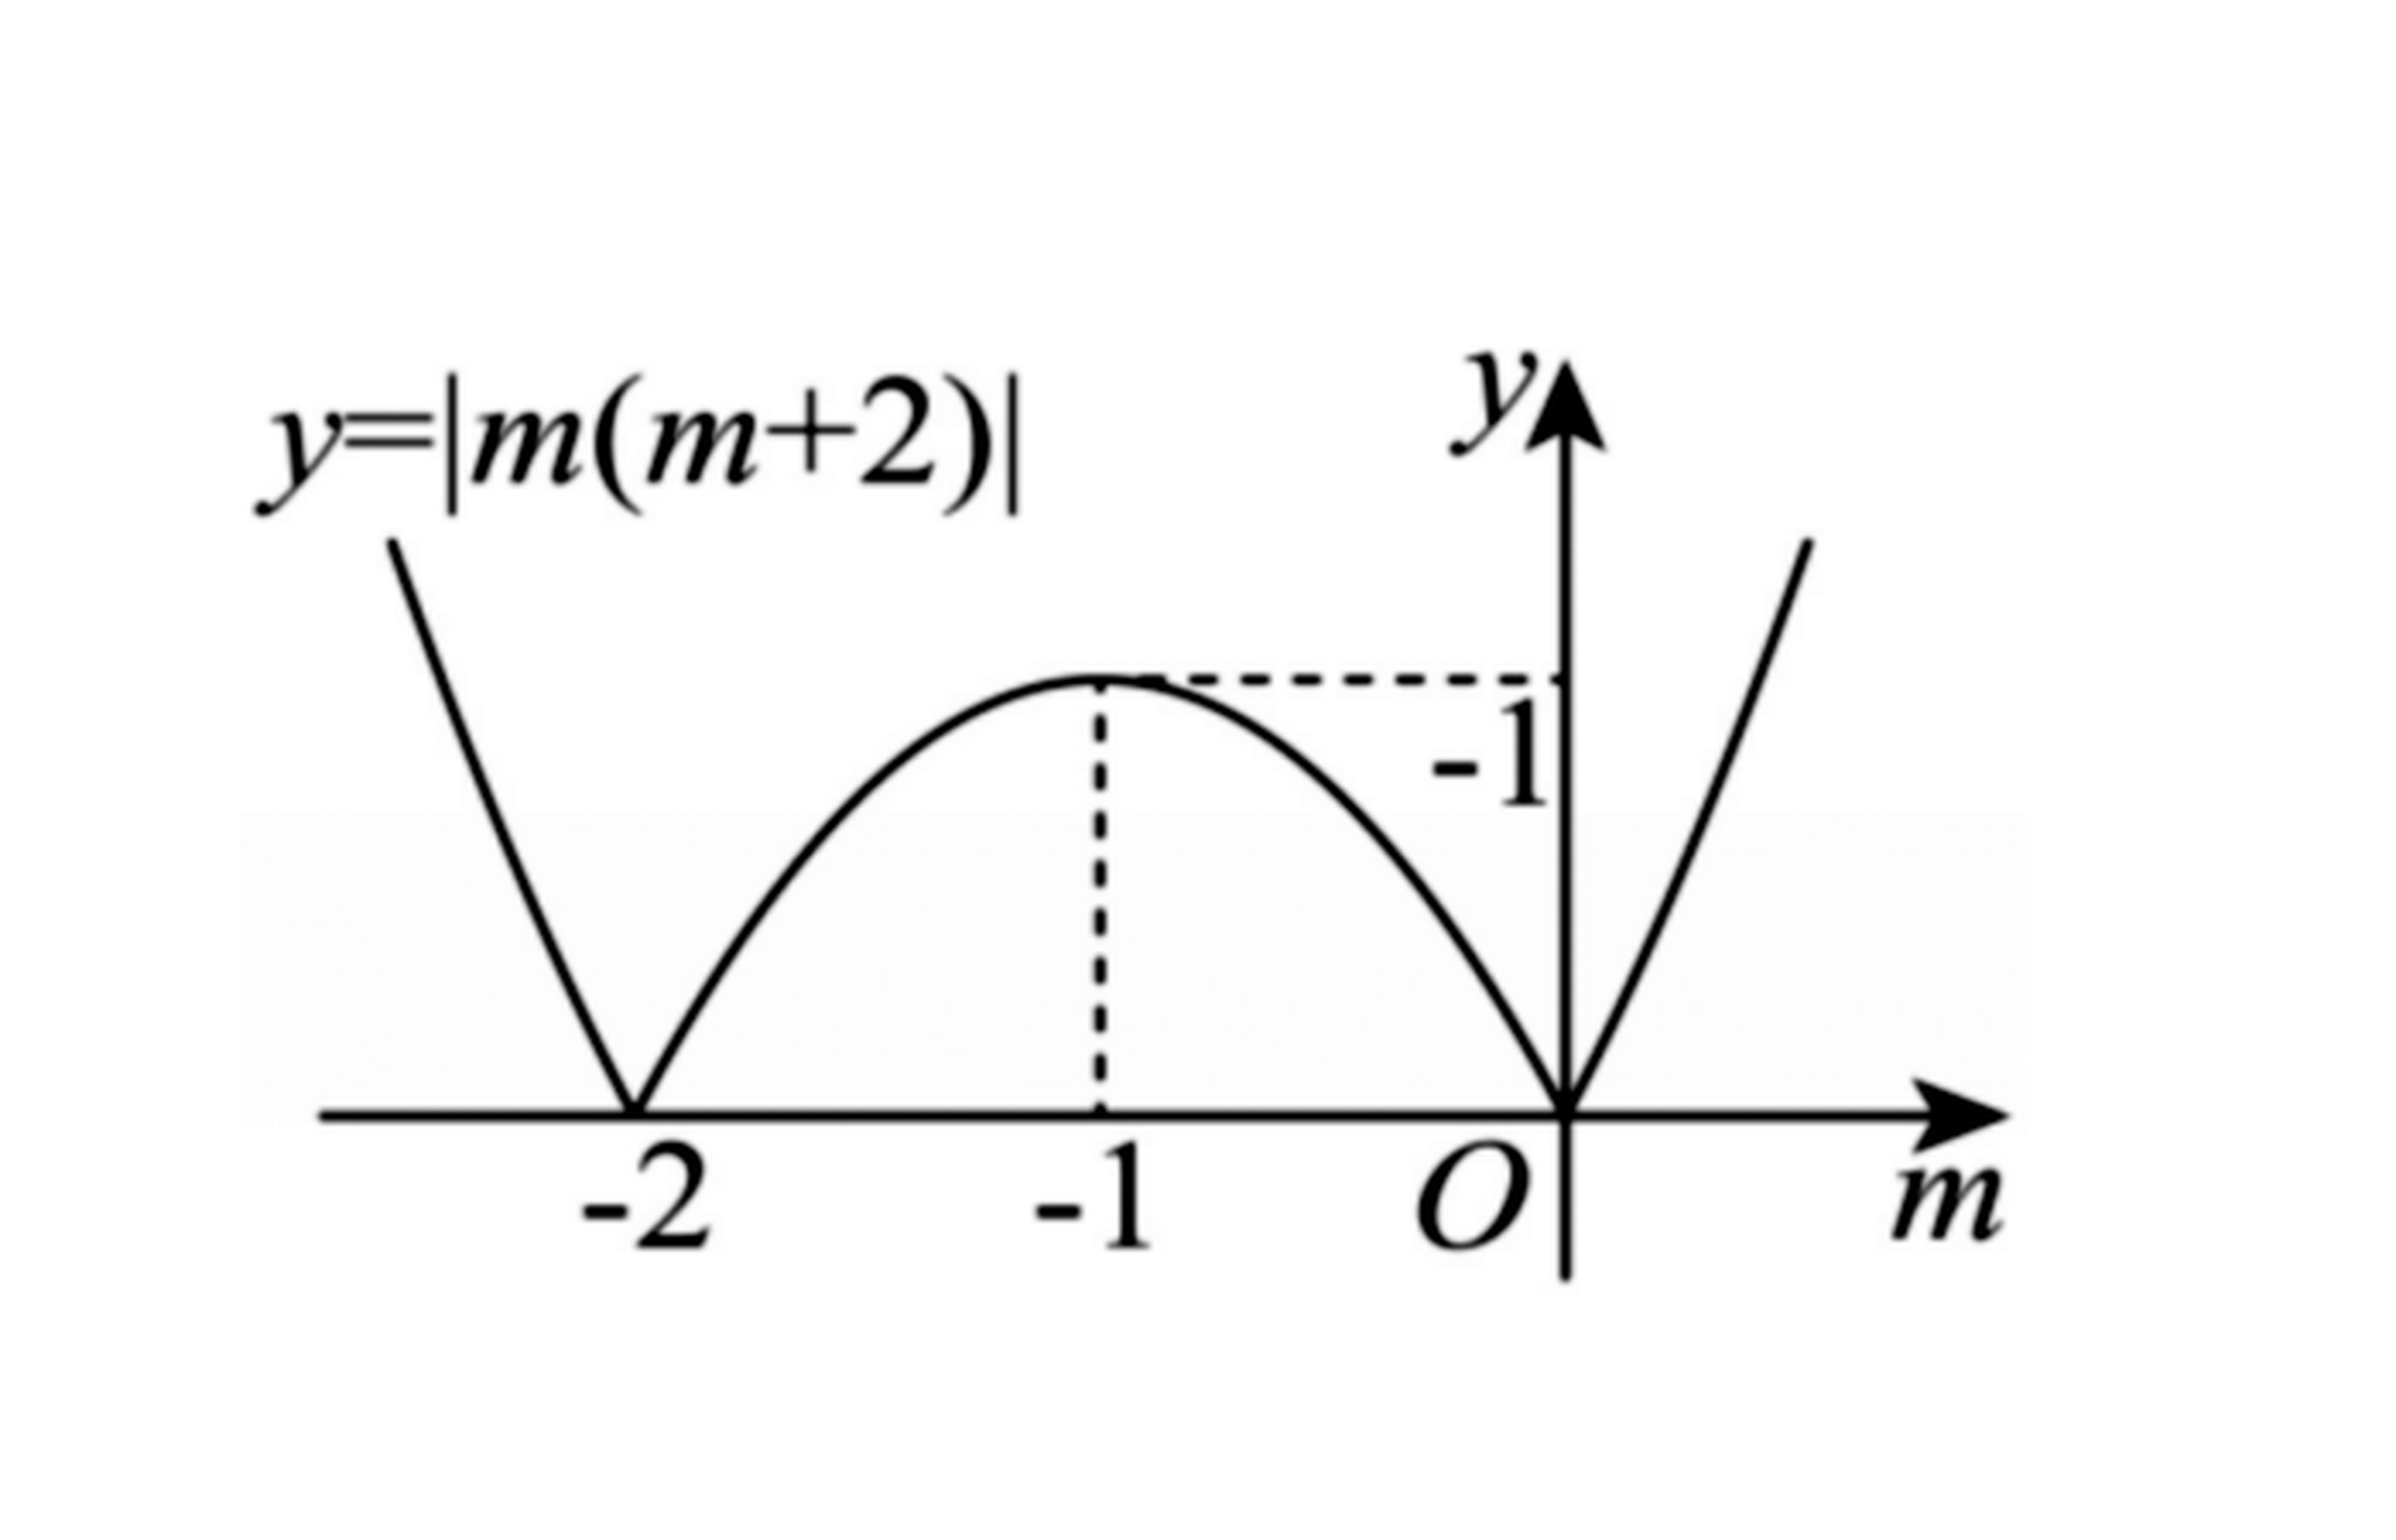
\includegraphics[width=0.46\textwidth]{figures/gao154_fujia2.png}
\end{center}
\step{由图像得 $k\in(0,1)$，}
\step{所以方程 $m^2+2m=k$ 和 $m^2+2m=-k$ 各有两个不同的根，}
\step{其中方程 $m^2+2m-k=0$ 的两根为 $m=-1\pm\sqrt{1+k}$，}
\step{方程 $m^2+2m+k=0$ 的两根为 $m=-1\pm\sqrt{1-k}$，}
\step{所以 $m_1=-1-\sqrt{1+k}$，$m_2=-1-\sqrt{1-k}$，$m_3=-1+\sqrt{1-k}$，$m_4=-1+\sqrt{1+k}$，且 $m_1<m_2<m_3<m_4$，}
\step{由 $m=\log_2 x$，则 $x=2^m$，}
\step{所以 $a=2^{-1-\sqrt{1+k}}$，$b=2^{-1-\sqrt{1-k}}$，$c=2^{-1+\sqrt{1-k}}$，$d=2^{-1+\sqrt{1+k}}$，}
\step{所以 $ad=2^{-1-\sqrt{1+k}}\times2^{-1+\sqrt{1+k}}=2^{(-1-\sqrt{1+k})+(-1+\sqrt{1+k})}=2^{-2}=\dfrac14$，}
\step{$b+c=2^{-1-\sqrt{1-k}}+2^{-1+\sqrt{1-k}}=\dfrac{2^{-\sqrt{1-k}}+2^{\sqrt{1-k}}}{2}$，}
\step{令 $s=\sqrt{1-k}$，其中 $s\in(0,1)$，则 $b+c=\dfrac12\left(2^{-s}+2^s\right)$，}
\step{设函数 $y=2^s+\dfrac1{2^s}$，令 $r=2^s\in(1,2)$，所以 $y=r+\dfrac1r$ 在 $(1,2)$ 上严格增，}
\step{所以函数 $y=2^s+\dfrac1{2^s}$ 在 $(0,1)$ 上严格增，所以 $y=2^s+\dfrac1{2^s}\in\left(2,\dfrac52\right)$，}
\step{所以 $b+c=\dfrac{2^{-s}+2^s}{2}\in\left(1,\dfrac54\right)$，$ad(b+c)=\dfrac{b+c}{4}\in\left(\dfrac14,\dfrac5{16}\right)$，}
\step{所以 $ad(b+c)$ 的取值范围是 $\left(\dfrac14,\dfrac5{16}\right)$，故选 $A$.}
\solend
\fi

\end{enumerate}

\end{document}
"
%
% ① 原始材料：微信公众号"魔都数学加油站"文章，连载"27学年高一154"，原文标题
% "27学年高一154——2026-2027年上海市徐汇中学高一上期中"；
% 原文链接：https://mp.weixin.qq.com/s/Qs2T7Zwsug-KKFE2wefDUg 。
% 正文为 12 张 PNG 页（01/03/04/05/07/11/12 为 2560×3620，
% 02/06/08/09/10 为 4762×6735，同一篇各页分辨率混排，逐页按各自分辨率裁图核对）。
% 体例：讲评版——一、填空题 3—12（10 题）、二、选择题 13—16（4 题）、
% 三、解答题 17—21（5 题）、附加题 1—2（2 题，原卷**另起编号**"1." "2."，
% 不与正题连号，同 高一a 成例），共 21 题；全卷每题均印【解析】
% （逐题核实，见 ② ②）。题目、答案、解析均据原图转录；卷面粉红色水印
% "魔都数学加油站"及公众号页脚未录入。
% 全卷插图清单（逐页通读 12 页确认）：3 组——
%   · Q15 题干配图（$f(x)=(x-a)(x-b)$ 抛物线，04 页右下：x/y 轴、O、1、
%     开口向上两零点均在 (0,1) 内），三版都出，裁 figures/gao154_q15_stem.png；
%   · Q15 四幅图像选项（05 页上半 2×2 排布，A/B/C/D 四幅指数函数图像，
%     合并成一张，照 高一136 Q13/Q22 成例），三版都出，
%     裁 figures/gao154_q15_opts.png；
%   · 附加题第 2 题解析配图（$y=\lvert m(m+2)\rvert$ 图像，11 页右上：
%     W 形折线、$-2$、$-1$、O、虚线 $y=1$ 与 $m=-1$），仅答案版出，
%     裁 figures/gao154_fujia2.png；
%   3 图均取自原卷截图，去粉色水印、去色、4× LANCZOS 放大；Q15 题干图
%   左侧题干残字"的图"已裁白。其余各页逐页确认无其它题目配图、无表格；
%   12 页下半仅水印、无正文。
%
% 卷首标题：原卷印作"2026-2027 年徐汇中学高一上期中"，年份区间按全稿惯例排 en dash；
% 原卷卷面未印副标题，本稿按同期中卷知识模块口径补出"集合与常用逻辑用语、不等式、函数"。
%
% ② 与原卷的排版差异：
%   ① 原文从第 3 题起，本稿保留原题号；共 21 题四节，正题到 21，附加题另起编号
%      1—2（\bigsec{附加题} 后 \begin{enumerate} 不 \setcounter，同 高一a 成例）；
%   ② 全 21 题均印【解析】、用 \solbegin…\solend，无只印【答案】或答案印括号内的题；
%      四道正题选择题答案在解析末句"故选 C／A／B／C"（Q13—Q16）、附加题第 2 题
%      答案在解析末句"故选 A"，括号 \mbox{（\quad）} 留空、不另提 \ans{}；
%      答案版【答案】/【解析】标记数 = 21 = 全卷题数；
%   ③ 原卷卷面未印副标题，本稿按知识模块口径补出；
%   ④ 原卷填空横线按全稿惯例排 \blankline[4.4em]；选择题括号排 \mbox{（\quad）}、
%      四道正题选择题与附加题第 2 题的选项段前按惯例各加 \keepwithprev
%      （Q15 与附加题 2 的选项段是整块图，\keepwithprev 后接 \begin{center}）；
%      解答题不留作答区、不加 \anspace（原卷为讲评版）；
%   ⑤ 数集黑板粗体：Q4"$x,y\in R$"、Q9"$x\in\R$"、Q13 无、
%      Q15"定义域 $\R$"、Q19"$\forall x\in\R$"、Q21"$x\in\N$"与"$k\in\N^*$"、
%      Q20"$a,b\in\R$"、附加题 2 无——原卷印斜体或正体粗体 R/N/N*，
%      按全稿惯例归一 \R／\N／\N^*；绝对值排 \lvert…\rvert
%      （Q5、Q9、Q12、Q13、Q16、Q21、附加题 2），集合描述竖线排 \mid
%      （Q5、Q17、Q19、Q21），不等号按全稿惯例排 \leqslant／\geqslant；
%      空集 \varnothing（Q21 题干 (3)）；
%   ⑥ 子集符号逐处照录、不得统一：Q6 题干印"$\{1,2\}\subset M\subseteq\{1,2,3,4,5\}$"
%      （前单线 ⊂、后带下划线 ⊆，同句两形并用），解析亦两形并用；
%      Q17 解析 (2)"$B\subset A$"印单线 ⊂；Q21 题干 (3)"$A\subseteq\{x\mid\cdots\}$"
%      印带下划线 ⊆——逐处放大核，分别 \subset／\subseteq，照录未统一（见 ④）；
%   ⑦ 判别式 Δ/△：Q18 解析 (1)"$\Delta=m^2-4(4m^2-3)$"与 Q19 解析 (1)
%      "$\Delta=4m^2-8m<0$"两处均印等腰偏高粗三角、照录 \Delta；本卷无扁等边
%      细线 \triangle 用例（见 ④）；
%   ⑧ 中文弯引号照录：Q4"设 $x$、$y\in\R$. 若 $x+y>2$，则 $x>1$ 或 $y>1$"、
%      附加题 1"$n$ 元集和集"与"3 元集和集"；注释里一律 ASCII 引号；
%      数学式内 CJK 用 \text{}（Q5 解集描述"或"、Q19 集合描述的"或"）；
%   ⑨ "图像／图象"逐处放大核：Q15 题干与解析印"图象"（象，无亻）、
%      Q16 无、附加题 2 解析印"图象"与"图像"（"画出函数…的图象"、
%      "由图像得"——两形并用，逐处照录未统一）；Q13/Q14 无数集图像字样；
%      半角逗号在数学组之间是全稿惯例、非笔误，逐处照录（Q3、Q10、Q16、
%      Q18、Q20、Q21 的 $x_1,x_2$ 之类）；行末西文句点 ASCII `.`；
%      行中全角逗号／顿号照录（Q6"3，4，5"、Q20"（单位：元）"、
%      附加题 1"$a_1,a_2,a_3,a_4$"）；
%   ⑩ 复杂式照录别简化：Q3 $a^{\frac{12}{7}}\cdot\left(\frac17\right)^{\frac17}
%      \cdot\sqrt[7]{a^4}$ 与 $7^{-\frac17}a^{\frac{16}{7}}$、Q7 $x^{-m}$、
%      Q8 $\frac{b-2a+2}{2a}$、Q11 $\frac{9+4\sqrt2}{6}$、Q12 $506\frac29$ 与
%      $506\frac49$、Q16 高斯取整 $[a]$、Q20 $c(x)=10x+\frac1{100}x^2$ 与
%      $q(x)=a+\frac xb$、Q21 $A^+$／$A^-$ 与 $|A^+|\geqslant2k-1$、
%      附加题 2 $m=-1\pm\sqrt{1+k}$ 与 $ad(b+c)$；
%      \left…\right 不得拆到不同 $…$ 组（Q5 $\left\{x\mid\cdots\right\}$、
%      Q20 $\left(\frac1b-\frac1{100}\right)$、附加题 2 $\left(\frac14,\frac5{16}\right)$）；
%      cases 块一律 \begin{cases}…\end{cases}；
%   ⑪ 一条 \step = 原卷解析的一个印刷行，cases 块整体算一个印刷行；别并折行、
%      别拆行。Q11 九行、Q12 六行、Q16 十六行、Q20 十一行、Q21 十七行、
%      附加题 2 十八行均按印刷行逐条断，不丢行；
%   ⑫ 配图：Q15 题干小图（三版都出）放 \item 内题干之后 \begin{center}，
%      Q15 四幅选项图（三版都出）放 \keepwithprev 之后的 \begin{center}，
%      Q15 用 \needvspace 守卫把"题干＋两图"整块推走（守卫放 \item 之前，
%      见 高一145 Q14/Q20 与 高一136 Q13 成例）；附加题 2 解析配图（仅答案版出）
%      放 \ifanswer 内 \solbegin…\solend 的 \step 之间（高一73 第 16 题成例）；
%   ⑬ 原卷解析内无红色"法一／法二"之类小标题，故本卷无 \stepm；红色水印
%      "魔都数学加油站"不录入；
%   ⑭ 跨页续印按题合并：见 ⑥；
%
% ③ 行数复核：一条 \step = 原卷解析的一个印刷行，cases 块作一个印刷行计。
%   逐题数（主会话逐页核对定稿）：Q3：1；Q4：1；Q5：3；Q6：4；Q7：3；
%   Q8：1；Q9：5；Q10：4；Q11：9；Q12：6；Q13：5；Q14：4；Q15：3；
%   Q16：16；Q17：5；Q18：9；Q19：10；Q20：11；Q21：17；
%   附加题 1：6；附加题 2：18。
%   合计 141 条 \step（本卷无 \stepm），与原卷逐题印刷行相等。全卷 21 题
%   均设 \solbegin…\solend，答案版【答案】/【解析】标记数 = 21 = 全卷题数。
%
% ④ 判别式／子集符号结论（逐处放大原图照录、不得统一，主会话像素级复核）：
%   判别式：Q18 解析 (1)"$\Delta=m^2-4(4m^2-3)=-15m^2+12\geqslant0$"、
%      Q19 解析 (1)"$\Delta=4m^2-8m<0$"共 2 处，逐处放大确认印等腰偏高
%      粗三角（高>宽、右斜边粗），照录 \Delta；本卷无扁等边细线 \triangle
%      用例，无几何三角形符号。
%   子集：Q6 题干"$\{1,2\}\subset M\subseteq\{1,2,3,4,5\}$"前 ⊂ 单线、
%      后 ⊆ 带下划线（/tmp/gao154/z/zoom/q6_subset.png），解析两处同样两形
%      并用，分别照录 \subset／\subseteq；Q17 解析 (2)"$B\subset A$"单线
%      照录 \subset；Q21 题干 (3)"$A\subseteq\{x\mid\cdots\}$"带下划线
%      照录 \subseteq。本卷 ⊂ 与 ⊆ 混用逐处照录、不得统一。
%      空集 \varnothing（Q21 题干 (3)）、数集 \R／\N／\N^* 归一见 ② ⑤。
%
% ⑤ 存疑照录（放大原图确认，照录未改、正文对应处另有 % 注）：
%   1. Q7 题干印 $f(x)=(3m-1)x^{-m}$，解析首句却写"幂函数 $f(x)=x^\alpha$
%      的系数必须为 1"（用 $\alpha$ 作指数记号），随后 $f(2)=2^\alpha=8$
%      得 $\alpha=3$、$f(x)=x^3$——题干指数 $-m$ 与解析 $\alpha$ 记法不同，
%      系原卷记号前后不一，逐处照录未统一（放大 01/02 页确认）。
%   2. Q11 解析"因为 $u>0,v>0$，由基本不等式得 $\frac{4v}{u}+\frac{2u}{v}
%      \geqslant2\sqrt{\frac{4v}{u}\cdot\frac{2u}{v}}=4\sqrt2$"与
%      "所以 $\frac4u+\frac1v=\frac16\left(\frac4u+\frac1v\right)(2u+v)$"
%      照录，未把 $u,v$ 化简回 $x,y$。
%   3. Q16 解析把"$[a]$ 表示不超过 $a$ 的最大整数"与"和至少有一个不小于 2"
%      连写在同一行（原卷如此），照录未改；末行"假设成立，C 正确，D 错误"照录。
%   4. Q18 解析 (2)"函数 $y=-7m^2+6$ 开口向下，对称轴为 $m=0$"却称求
%      "$y_{\min}$"（实为在 $m^2\leqslant\frac45$ 闭区间上的最小值），
%      照录未改。
%   5. Q20 题干"$q(x)=a+\frac xb$（$a,b\in\R$）"与解析
%      "$W(x)=\left(\frac1b-\frac1{100}\right)x^2+(a-10)x-160000$"照录；
%      末行解得 $a=90,b=\frac{500}{3}$ 照录未化简。
%   6. Q21 题干 (3)"$A\subseteq\{x\mid0\leqslant x\leqslant2020,x\in\N\}$"
%      与解析"$3k-1\leqslant2a_k+1\leqslant4041$（$k\in\N^*$）"照录；
%      末行"集合 $A$ 中元素的个数的最大值是 1347"照录。
%   7. 附加题 1 解析"相加化简得 $a_1+a_2+a_3+a_4=5$"照录；
%      附加题 2 解析"由图像得 $k\in(0,1)$"与"由图像得"／"的图象"两形
%      并用逐处照录（见 ② ⑨）；末行"$ad(b+c)$ 的取值范围是
%      $\left(\frac14,\frac5{16}\right)$，故选 A"照录。
%   全卷除此 7 类外未发现其它笔误／自相矛盾处；21 题均印【解析】、
%   无只印【答案】或答案印括号内的题（见 ② ②）。
%
% ⑥ 跨页续印按题合并说明（逐页核实定稿）：Q3—Q5 题干＋解析在 01 页
%   （Q5 解析末 2 行续 01 页下半）；Q6、Q7 题干＋解析在 01 页下半
%   （Q7 解析余 2 行续 02 页顶）；Q8、Q9 题干＋解析在 02 页上半
%   （Q9 解析余 3 行续 02 页下半）；Q10 题干＋解析在 02 页下半；
%   Q11 题干＋解析前 6 行在 03 页上半、余 3 行续 03 页下半；
%   Q12 题干＋解析前 5 行在 03 页下半、末行续 04 页顶；"二、选择题"
%   标题与 Q13 题干＋选项＋解析在 04 页上半；Q14 题干＋选项＋解析、
%   Q15 题干＋题干配图在 04 页下半；Q15 四幅选项图＋解析、
%   Q16 题干＋选项＋解析首行在 05 页上半，Q16 解析余 12 行在
%   05 页下半—06 页上半；"三、解答题"标题与 Q17 题干＋两问＋解析
%   在 06 页下半；Q18 题干＋两问＋解析在 07 页上半—下半；
%   Q19 题干＋两问＋解析首行在 07 页下半，解析余 8 行在 08 页上半；
%   Q20 题干在 08 页下半，解析 (1) 4 行＋(2) 首 4 行在 08 页下半—09 页上半，
%   (2) 余 2 行在 09 页下半；Q21 题干＋三问＋解析 (1)(2) 4 行在
%   09 页下半—10 页上半，解析 (3) 余 12 行在 10 页上半—下半；
%   "附加题"标题与附加题 1 题干＋解析首 3 行在 10 页下半，
%   余 3 行续 11 页上半；附加题 2 题干＋选项＋解析前 3 行在 11 页上半，
%   解析配图＋余 12 行在 11 页下半—12 页上半，末行
%   "所以 $ad(b+c)$ 的取值范围是 $\left(\frac14,\frac5{16}\right)$，故选 A"
%   为全卷收尾（12 页下半仅水印、无正文）。
%   本稿按题连排，不丢行、不并折行；全卷末题为附加题第 2 题。
%
\documentclass[a4paper,11pt]{article}
\usepackage{common}

\begin{document}

\examtitlest[3]{2026--2027 年徐汇中学高一上期中}{集合与常用逻辑用语、不等式、函数}

\bigsec{一、填空题}

\begin{enumerate}
\setcounter{enumi}{2}

% === Q3 === 分数指数幂照录；解析 1 行
\item 已知 $a>0$，化简 $a^{\frac{12}{7}}\cdot\left(\dfrac17\right)^{\frac17}\cdot\sqrt[7]{a^4}=$\blankline[4.4em].

\ifanswer
\solbegin
\step{$a^{\frac{12}{7}}\cdot\left(\dfrac17\right)^{\frac17}\cdot\sqrt[7]{a^4}=a^{\frac{12}{7}}\cdot(7^{-1})^{\frac17}\cdot a^{\frac47}=7^{-\frac17}a^{\frac{16}{7}}$.}
\solend
\fi

% === Q4 === 反证法；中文弯引号照录；解析 1 行
\item 用反证法证明命题：“设 $x$、$y\in\R$. 若 $x+y>2$，则 $x>1$ 或 $y>1$”时，假设的内容应该是\blankline[4.4em].

\ifanswer
\solbegin
\step{由反证法得，假设的内容应该是 $x\leqslant1$ 且 $y\leqslant1$.}
\solend
\fi

% === Q5 === 分式不等式；cases 块；解析 3 行
\item 不等式 $\dfrac{2x+3}{x-1}\geqslant1$ 的解集为\blankline[4.4em].

\ifanswer
\solbegin
\step{$\dfrac{2x+3}{x-1}\geqslant1$，即 $\dfrac{2x+3}{x-1}-1\geqslant0$，$\dfrac{x+4}{x-1}\geqslant0$，}
\step{等价于 $\begin{cases}(x+4)(x-1)\geqslant0\\x-1\ne0\end{cases}$，解得 $x>1$ 或 $x\leqslant-4$，}
\step{故解集为 $\{x\mid x>1\text{ 或 }x\leqslant-4\}$.}
\solend
\fi

% === Q6 === ⊂ 与 ⊆ 并用照录；解析 4 行
\item 满足条件 $\{1,2\}\subset M\subseteq\{1,2,3,4,5\}$ 的集合 $M$ 的个数为\blankline[4.4em].

\ifanswer
\solbegin
\step{因为 $\{1,2\}\subset M\subseteq\{1,2,3,4,5\}$，所以集合 $M$ 必含有元素 1，2，}
\step{且至少含有元素 3，4，5 中的一个，}
\step{则集合 $M$ 的个数与集合 $\{3,4,5\}$ 的非空子集的个数一样，}
\step{所以集合 $M$ 的个数为 $2^3-1=7$.}
\solend
\fi

% === Q7 === 题干 $x^{-m}$、解析用 $x^\alpha$ 记法，原卷记号差异照录（见 ⑤ 1）；解析 3 行
\item 已知幂函数 $f(x)=(3m-1)x^{-m}$，且 $f(2)=8$，则 $f(m)=$\blankline[4.4em].

\ifanswer
\solbegin
\step{幂函数 $f(x)=x^\alpha$ 的系数必须为 1，所以 $3m-1=1$，得 $m=\dfrac23$.}
\step{又 $f(2)=2^\alpha=8=2^3$，故 $\alpha=3$，即 $f(x)=x^3$，}
\step{所以 $f(m)=f\left(\dfrac23\right)=\left(\dfrac23\right)^3=\dfrac8{27}$.}
\solend
\fi

% === Q8 === 换底公式；解析 1 行
\item 已知 $a=\lg2$，$b=\lg3$，用含 $a,b$ 的代数式表示 $\log_4 75=$\blankline[4.4em].

\ifanswer
\solbegin
\step{$\log_4 75=\dfrac{\lg\left(3\times\frac{10^2}{2^2}\right)}{\lg2^2}=\dfrac{\lg3+2-2\lg2}{2\lg2}=\dfrac{b-2a+2}{2a}$.}
\solend
\fi

% === Q9 === 三角不等式取等；解析 5 行
\item 设 $x\in\R$，则方程 $\lvert x-2\rvert+\lvert3x+1\rvert=\lvert2x+3\rvert$ 的解集是\blankline[4.4em].

\ifanswer
\solbegin
\step{由 $\lvert x-2\rvert=\lvert2-x\rvert$，故原方程可化为 $\lvert2-x\rvert+\lvert3x+1\rvert=\lvert2x+3\rvert$，}
\step{又 $(2-x)+(3x+1)=2x+3$，}
\step{由三角不等式 $\lvert2-x\rvert+\lvert3x+1\rvert\geqslant\lvert(2-x)+(3x+1)\rvert=\lvert2x+3\rvert$，}
\step{当且仅当 $(2-x)(3x+1)\geqslant0$ 等号成立，}
\step{解 $(2-x)(3x+1)\geqslant0$ 得 $-\dfrac13\leqslant x\leqslant2$，故原方程的解集为 $\left[-\dfrac13,2\right]$.}
\solend
\fi

% === Q10 === 韦达定理；cases 块；解析 4 行
\item 已知一元二次不等式 $x^2+bx+c>0$ 的解集为 $(-\infty,-1)\cup(2,+\infty)$，则一元二次不等式 $bx^2+cx-1<0$ 的解集是\blankline[4.4em].

\ifanswer
\solbegin
\step{因为 $x^2+bx+c>0$ 的解集为 $(-\infty,-1)\cup(2,+\infty)$，}
\step{所以方程 $x^2+bx+c=0$ 的两根为 $-1$ 和 2，则有 $\begin{cases}-b=-1+2\\c=-1\times2\end{cases}$，即 $\begin{cases}b=-1\\c=-2\end{cases}$，}
\step{则 $bx^2+cx-1<0$ 等价于 $-x^2-2x-1<0$，得 $x^2+2x+1>0$，得 $(x+1)^2>0$，}
\step{解得 $x\ne-1$，故不等式 $bx^2+cx-1<0$ 的解集为 $(-\infty,-1)\cup(-1,+\infty)$.}
\solend
\fi

% === Q11 === 换元 $u,v$；解析 9 行
\item 已知正数 $x,y$ 满足 $2x+y=1$，则 $\dfrac4{x+2}+\dfrac1{y+1}$ 的最小值为\blankline[4.4em].

\ifanswer
\solbegin
\step{令 $u=x+2$，$v=y+1$，则 $u>2$，$v>1$，}
\step{且 $2u+v=2(x+2)+(y+1)=2x+y+5=6$.}
\step{因为 $u>0$，$v>0$，由基本不等式得 $\dfrac{4v}{u}+\dfrac{2u}{v}\geqslant2\sqrt{\dfrac{4v}{u}\cdot\dfrac{2u}{v}}=4\sqrt2$，}
\step{所以 $\dfrac4u+\dfrac1v=\dfrac16\left(\dfrac4u+\dfrac1v\right)(2u+v)=\dfrac16\left(9+\dfrac{4v}{u}+\dfrac{2u}{v}\right)\geqslant\dfrac{9+4\sqrt2}{6}$，}
\step{当且仅当 $\dfrac{4v}{u}=\dfrac{2u}{v}$，即 $u=\sqrt2v$ 时等号成立，}
\step{与 $2u+v=6$ 联立得 $u=\dfrac{6\sqrt2}{2\sqrt2+1}$，$v=\dfrac6{2\sqrt2+1}$，}
\step{此时 $x=u-2=\dfrac{2\sqrt2-2}{2\sqrt2+1}>0$，$y=v-1=\dfrac{5-2\sqrt2}{2\sqrt2+1}>0$，且 $2x+y=1$，}
\step{满足题设，所以下界可以取得，}
\step{因此 $\dfrac4{x+2}+\dfrac1{y+1}$ 的最小值为 $\dfrac{9+4\sqrt2}{6}$.}
\solend
\fi

% === Q12 === 2025 个整数解；解析 6 行
\item 若关于 $x$ 的不等式 $\lvert x-2k\rvert+\lvert x-3k\rvert<4k$ 共有 2025 个整数解，则实数 $k$ 的取值范围为\blankline[4.4em].

\ifanswer
\solbegin
\step{显然 $k>0$，由 $\lvert x-2k\rvert+\lvert x-3k\rvert<4k$，得 $\dfrac12k<x<\dfrac92k$，}
\step{因为该不等式共有 2025 个整数解，所以 $2024<\dfrac{9k}{2}-\dfrac k2\leqslant2026$，}
\step{解得 $506<k\leqslant506.5$，}
\step{由 $\dfrac k2\in(253,253.25]$，得这 2025 个整数解只能为 254、255、256、$\cdots$、2278，}
\step{所以 $2278<\dfrac{9k}{2}\leqslant2279$，解得 $506\dfrac29<k\leqslant506\dfrac49$，结合 $506<k\leqslant506.5$，}
\step{得 $k$ 的取值范围是 $\left(506\dfrac29,506\dfrac49\right]$.}
\solend
\fi

\end{enumerate}

\bigsec{二、选择题}

\begin{enumerate}
\setcounter{enumi}{12}

% === Q13 === 四选项一行；解析 5 行，故选 C
\item 若 $a<b<0$，则下列不等式中不成立的是\mbox{（\quad）}

\keepwithprev
A. $a-b>a$\qquad B. $\dfrac1a>\dfrac1b$\qquad C. $a^3>b^3$\qquad D. $\lvert a\rvert>\lvert b\rvert$

\ifanswer
\solbegin
\step{A 选项，因为 $b<0$，所以 $-b>0$，不等式两边同加上 $a$ 得 $a-b>a$，故 A 正确；}
\step{B 选项，因为 $a<b<0$，所以 $ab>0$，不等式两边同除以 $ab$，则 $\dfrac1b<\dfrac1a<0$，故 B 正确；}
\step{C 选项，不妨设 $a=-2$，$b=-1$，则 $a^3=-8$，$b^3=-1$，故 $a^3<b^3$，故 C 错误；}
\step{D 选项，因为 $a<b<0$，所以 $-a>-b$，即 $\lvert a\rvert>\lvert b\rvert$，故 D 正确.}
\step{故选 $C$.}
\solend
\fi

% === Q14 === 选项两行两列；解析 4 行，故选 A
\item 设命题 $p:x^2-5x+4\ne0$，命题 $q:x\ne1$，则 $p$ 是 $q$ 的\mbox{（\quad）}条件

\keepwithprev
A. 充分不必要\qquad\qquad B. 必要不充分

C. 充要\qquad\qquad D. 既不充分也不必要

\ifanswer
\solbegin
\step{$p:x^2-5x+4\ne0\Leftrightarrow(x-1)(x-4)\ne0\Leftrightarrow x\ne1$ 且 $x\ne4$；$q:x\ne1$.}
\step{充分性：当 $x\ne1$ 且 $x\ne4$ 时，$x\ne1$，所以 $p\Rightarrow q$；}
\step{必要性：当 $x\ne1$ 时，若 $x=4$，此时 $p$ 不成立，即 $q\nRightarrow p$；}
\step{所以 $p$ 是 $q$ 的充分不必要条件，故选 $A$.}
\solend
\fi

% === Q15 === 题干配图（三版都出）+ 四幅图像选项（2×2 合并，三版都出）；守卫放 \item 之前；解析 3 行，故选 B
\needvspace{9cm}
\item 已知函数 $f(x)=(x-a)(x-b)$（$a<b$）的图象如图所示，则函数 $g(x)=a^x-b$ 的图象可能是\mbox{（\quad）}

\begin{center}
% 抛物线题干配图取 04 页右下，去粉色水印、去色、4× LANCZOS 放大；三版都出
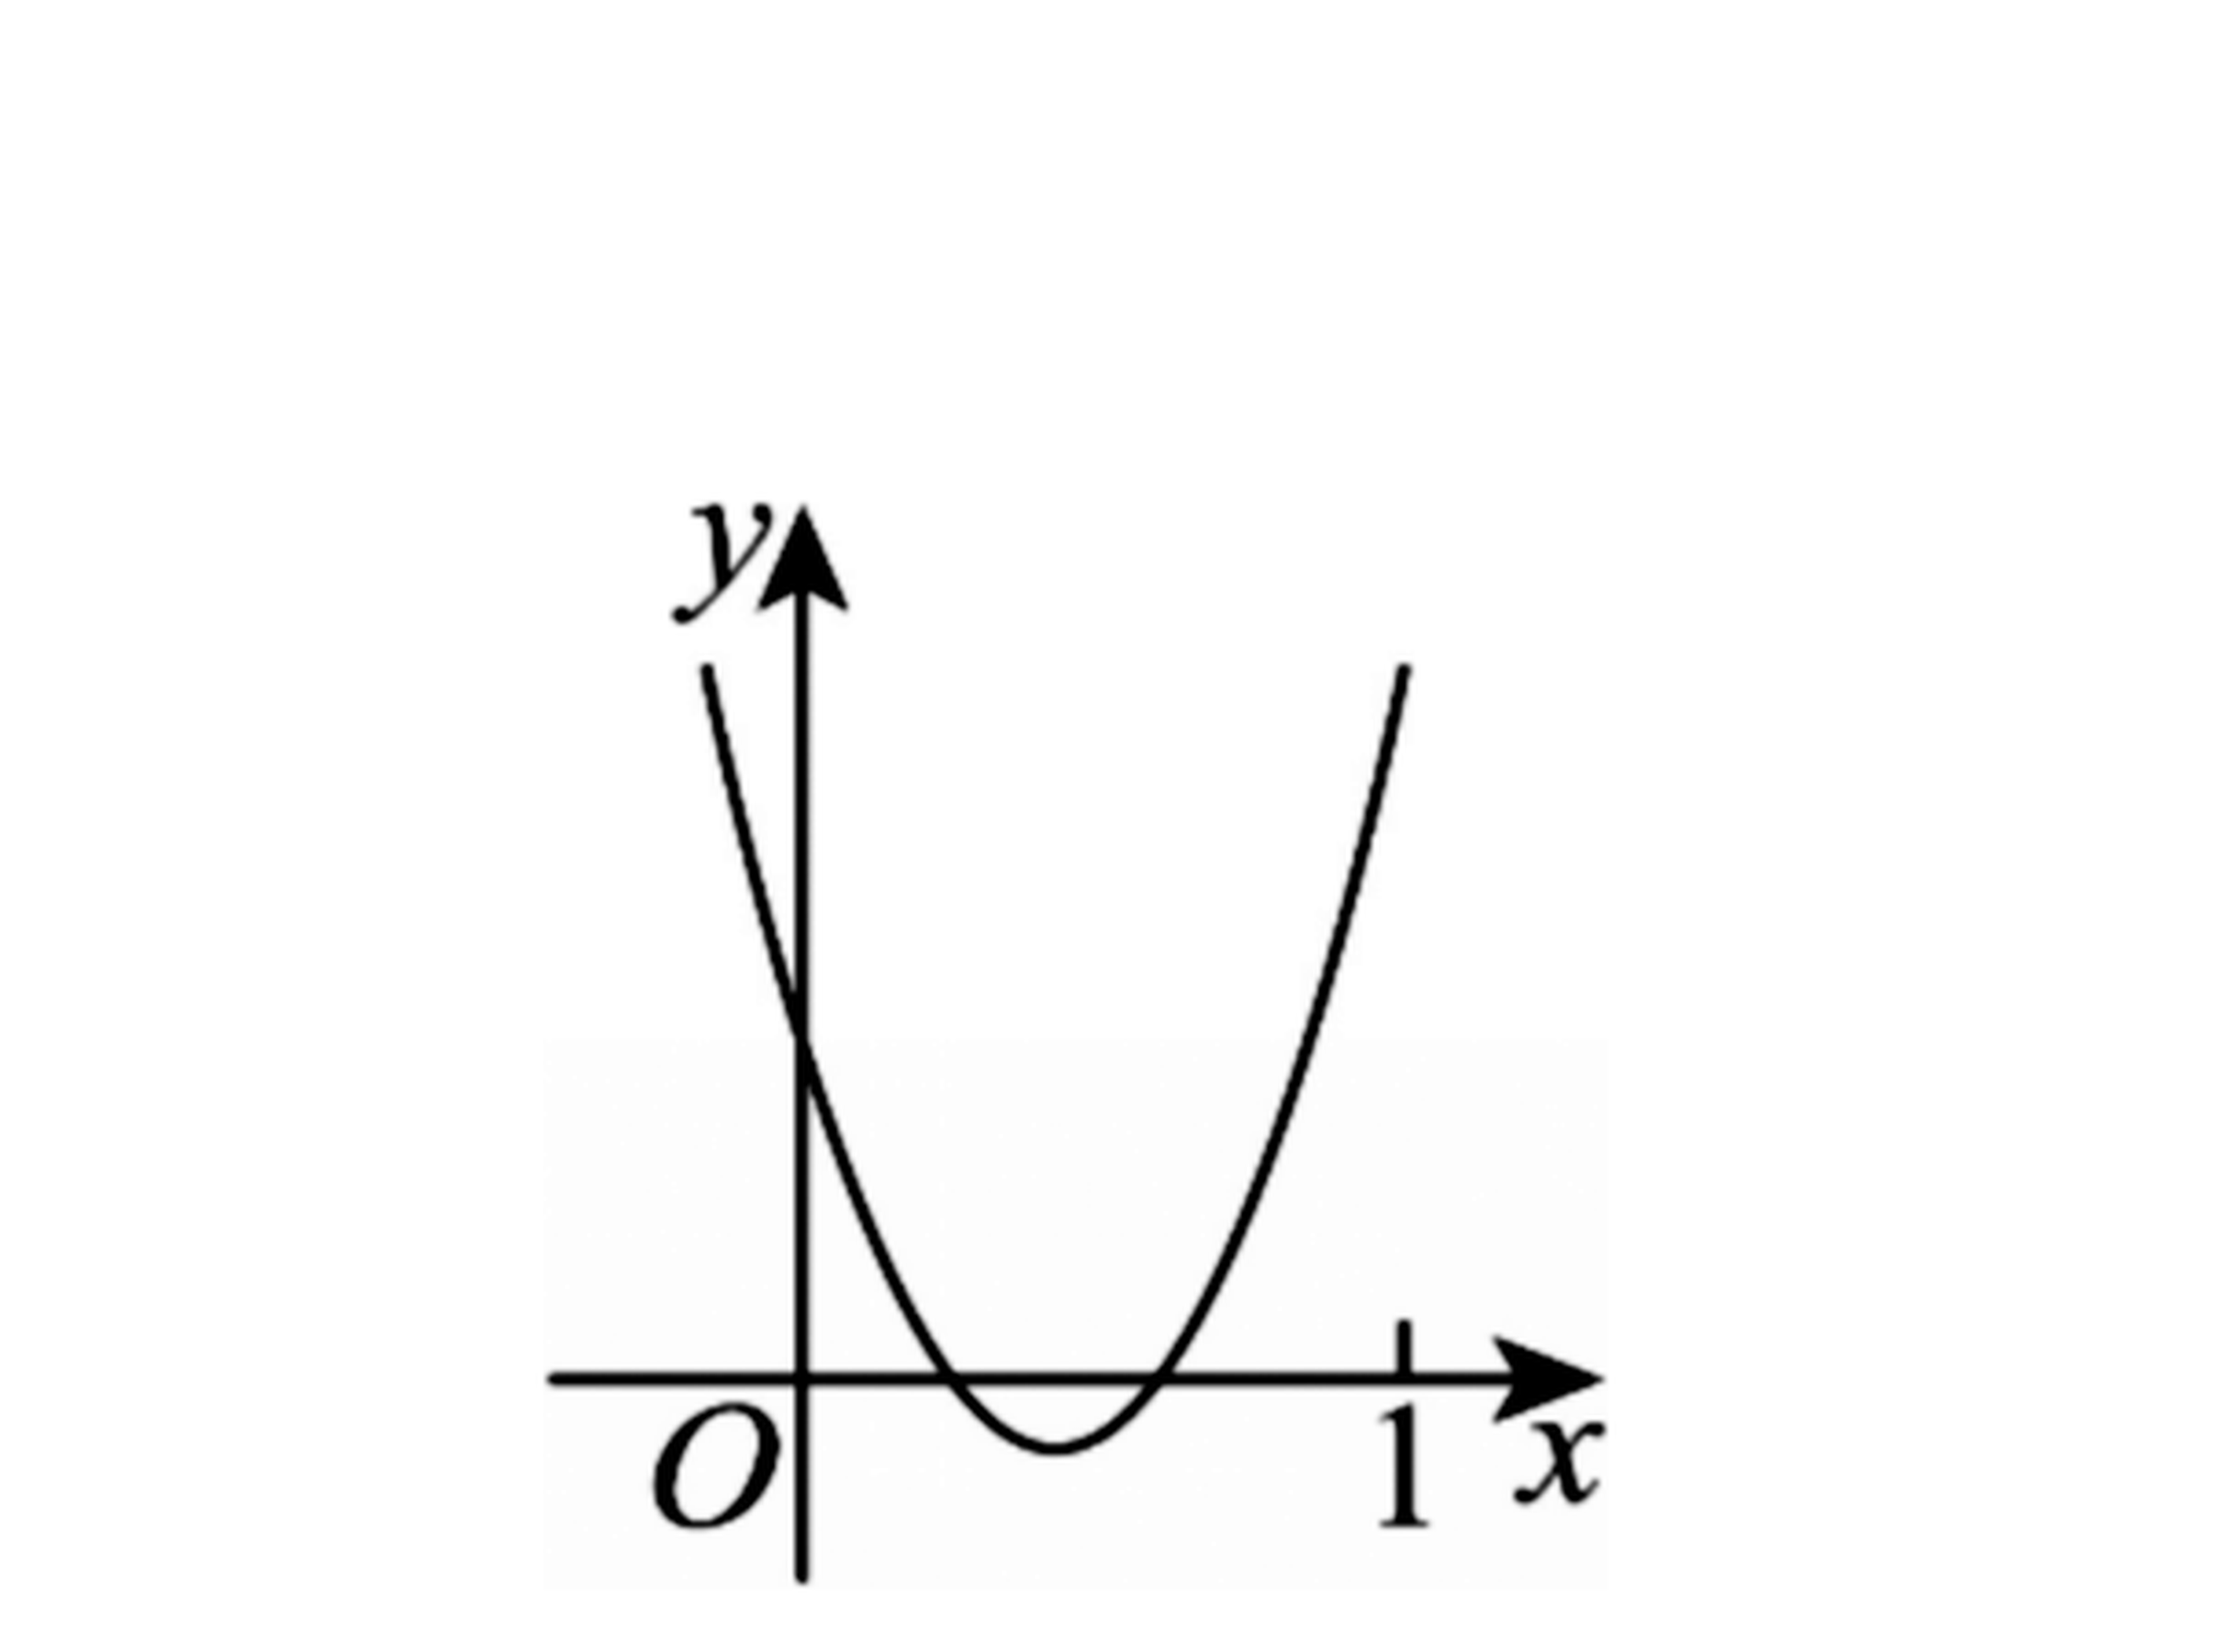
\includegraphics[width=0.32\textwidth]{figures/gao154_q15_stem.png}
\end{center}

\keepwithprev
\begin{center}
% 四幅指数函数图像选项取 05 页上半，按原卷 2×2 排布合并为一张，去粉色水印、去色、4× LANCZOS 放大；三版都出
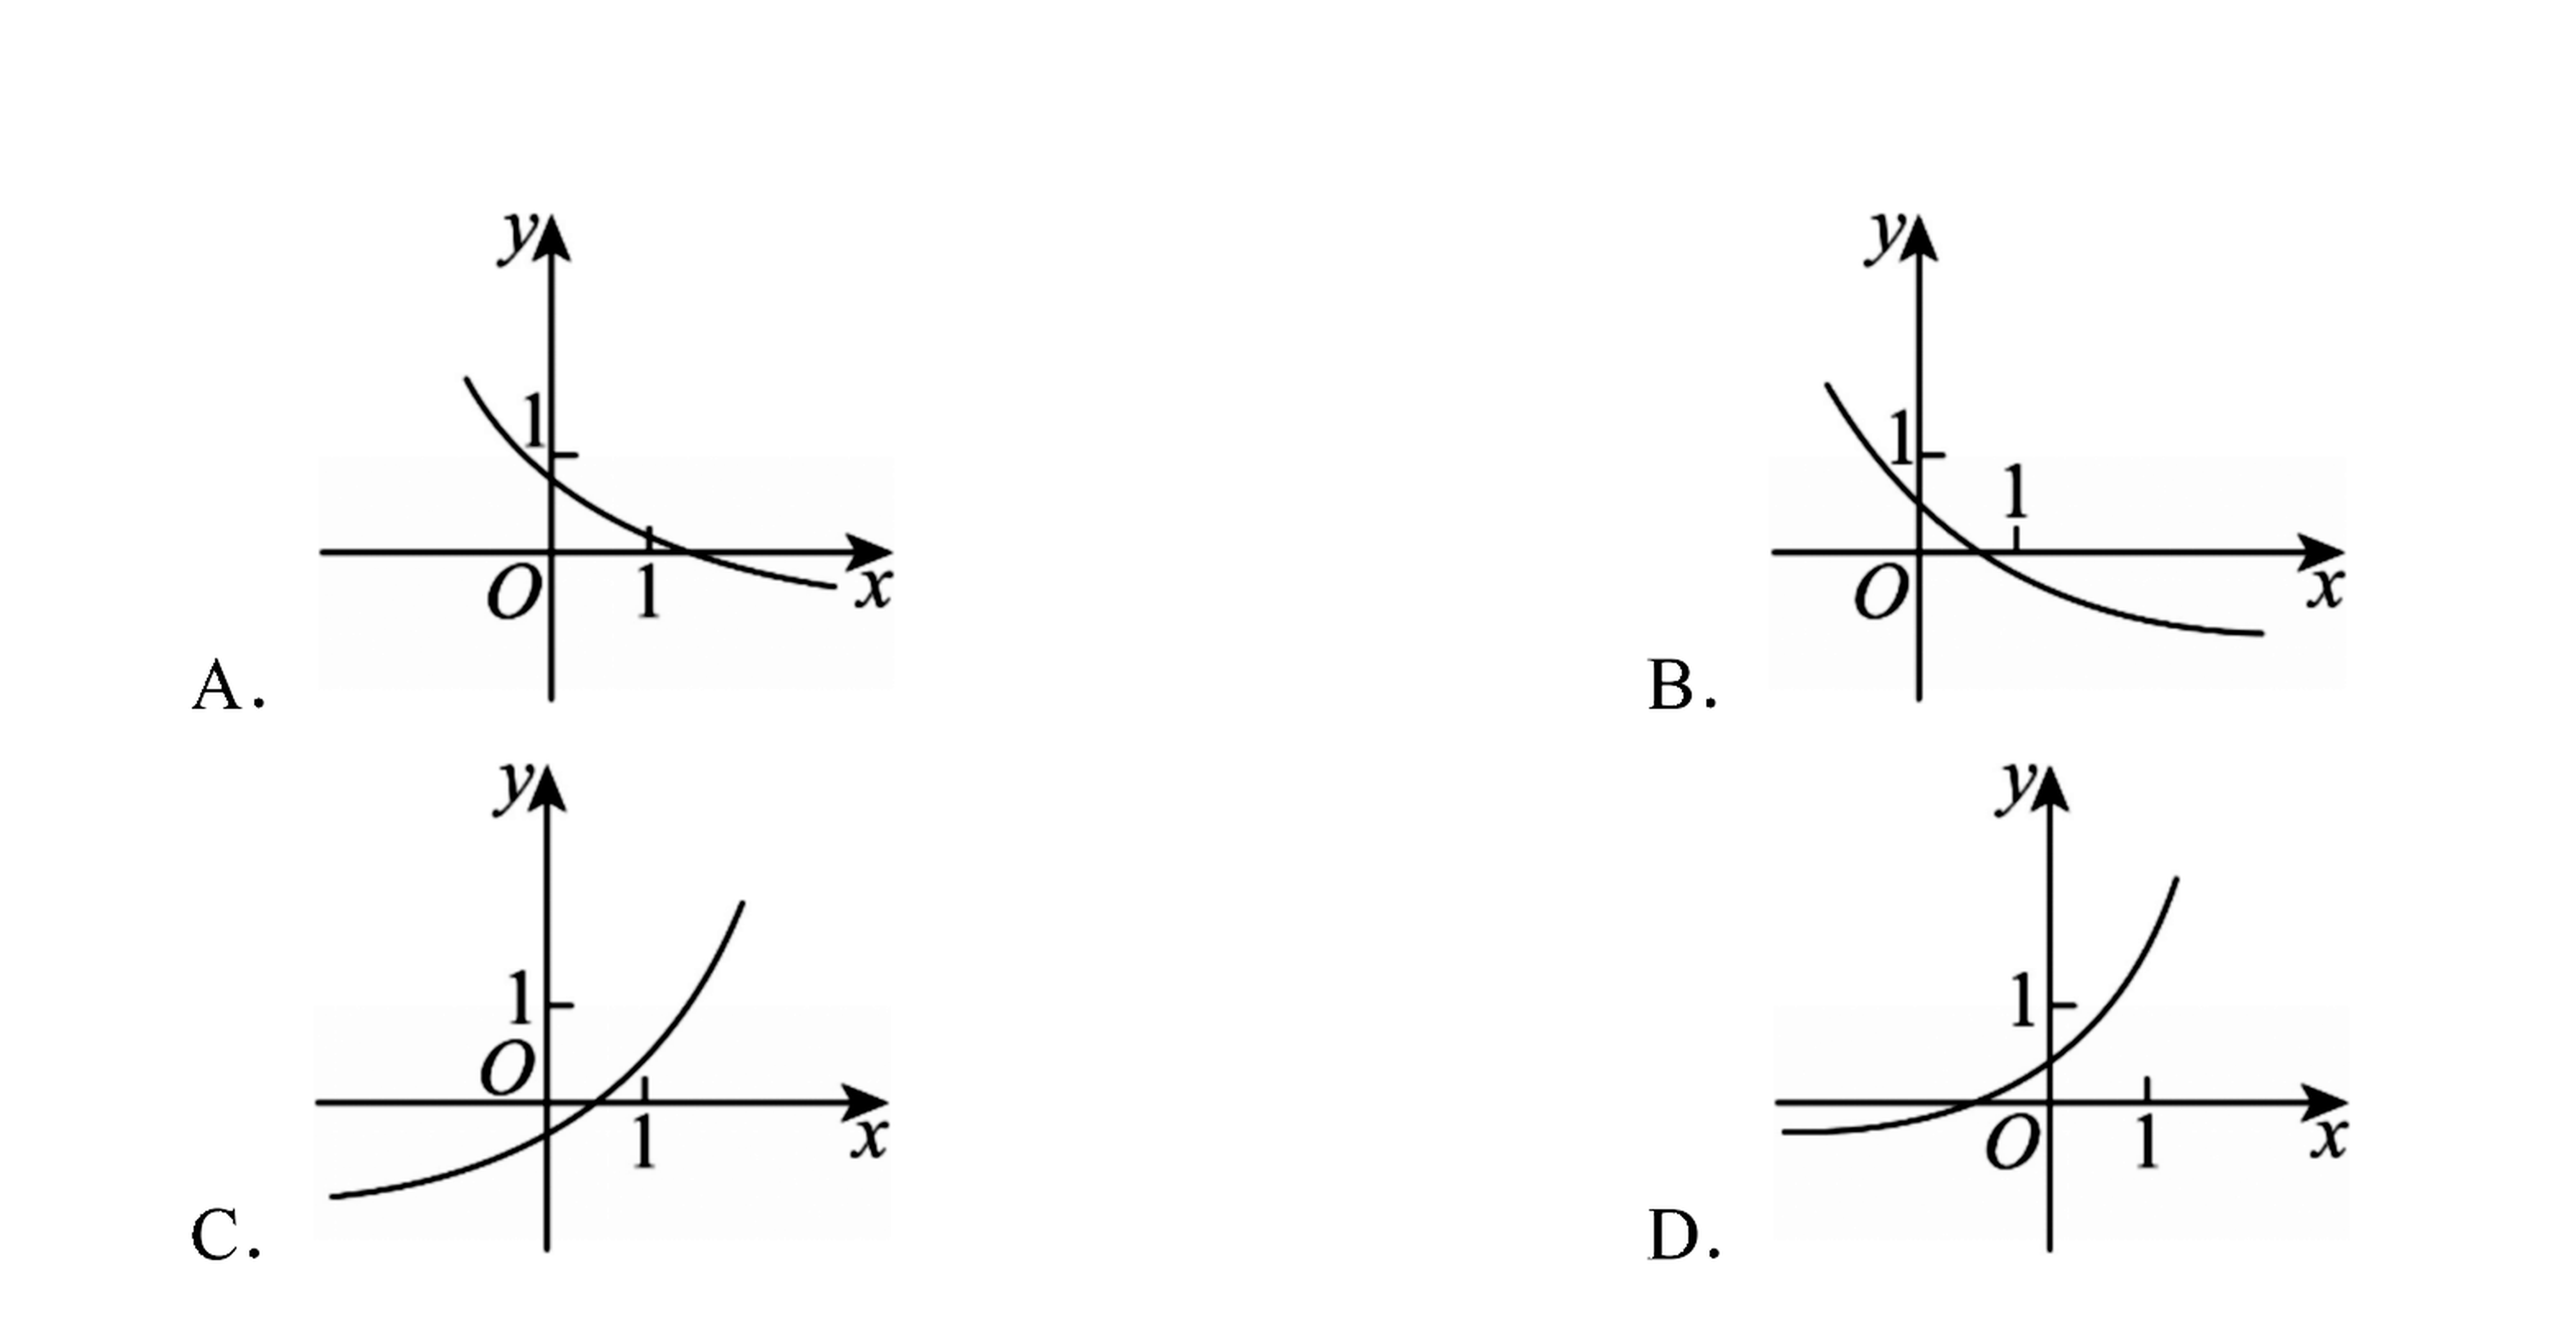
\includegraphics[width=0.80\textwidth]{figures/gao154_q15_opts.png}
\end{center}

\ifanswer
\solbegin
\step{由题意得 $0<a<b<1$，所以 $g(x)=a^x-b$ 在定义域 $\R$ 上严格减.}
\step{$g(0)=a^0-b=1-b>0$，$g(1)=a^1-b=a-b<0$，故 B 符合题意.}
\step{故选 $B$.}
\solend
\fi

% === Q16 === 高斯取整；解析 13 行，故选 C
\item 设 $[a]$ 表示不超过 $a$ 的最大整数，如 $[1.2]=1$，$[-3.2]=-4$，若 $x$、$y$、$z$ 为正实数，则 $\left[\dfrac{y+z}{x}\right]+\left[\dfrac{z+x}{y}\right]+\left[\dfrac{x+y}{z}\right]$ 的最小值为\mbox{（\quad）}

\keepwithprev
A. 2\qquad\qquad B. 3\qquad\qquad C. 4\qquad\qquad D. 6

\ifanswer
\solbegin
\step{若 $x$、$y$、$z$ 为正实数，}
\step{结合基本不等式得 $\dfrac{y+z}{x}+\dfrac{z+x}{y}+\dfrac{x+y}{z}=\dfrac yx+\dfrac xy+\dfrac zx+\dfrac xz+\dfrac zy+\dfrac yz$}
\step{$\geqslant2\sqrt{\dfrac yx\cdot\dfrac xy}+2\sqrt{\dfrac zx\cdot\dfrac xz}+2\sqrt{\dfrac zy\cdot\dfrac yz}=6$，当且仅当 $x=y=z$ 时取等号，}
\step{即 $\dfrac{y+z}{x}$，$\dfrac{z+x}{y}$，$\dfrac{x+y}{z}$ 中至少有一个不小于 2，不妨设 $\dfrac{y+z}{x}\geqslant\dfrac{z+x}{y}\geqslant\dfrac{x+y}{z}$，}
\step{$[a]$ 表示不超过 $a$ 的最大整数和 $\dfrac{y+z}{x}$，$\dfrac{z+x}{y}$，$\dfrac{x+y}{z}$ 中至少有一个不小于 2，}% 原卷此行把两句连写，照录未改（见 ⑤ 3）
\step{得 $\left[\dfrac{y+z}{x}\right]\geqslant2$，所以 $\left[\dfrac{y+z}{x}\right]+\left[\dfrac{z+x}{y}\right]+\left[\dfrac{x+y}{z}\right]\geqslant2$，}
\step{假设 $\left[\dfrac{y+z}{x}\right]+\left[\dfrac{z+x}{y}\right]+\left[\dfrac{x+y}{z}\right]$ 的最小值为 2，$\left[\dfrac{y+z}{x}\right]=2$，$\left[\dfrac{z+x}{y}\right]+\left[\dfrac{x+y}{z}\right]=0$，}
\step{所以 $2\leqslant\dfrac{y+z}{x}<3$，$0<\dfrac{z+x}{y}<1$，$0<\dfrac{x+y}{z}<1$，所以 $2<\dfrac{y+z}{x}+\dfrac{z+x}{y}+\dfrac{x+y}{z}<5$，}
\step{与 $\dfrac{y+z}{x}+\dfrac{z+x}{y}+\dfrac{x+y}{z}\geqslant6$ 矛盾，假设不成立，A 错误；}
\step{假设 $\left[\dfrac{y+z}{x}\right]+\left[\dfrac{z+x}{y}\right]+\left[\dfrac{x+y}{z}\right]$ 的最小值为 3，}
\step{则 $\left[\dfrac{y+z}{x}\right]=2$，$\left[\dfrac{z+x}{y}\right]=1$，$\left[\dfrac{x+y}{z}\right]=0$ 或 $\left[\dfrac{y+z}{x}\right]=3$，$\left[\dfrac{z+x}{y}\right]=\left[\dfrac{x+y}{z}\right]=0$，}
\step{同理可得 $3<\dfrac{y+z}{x}+\dfrac{z+x}{y}+\dfrac{x+y}{z}<6$，显然不成立，B 错误；}
\step{假设 $\left[\dfrac{y+z}{x}\right]+\left[\dfrac{z+x}{y}\right]+\left[\dfrac{x+y}{z}\right]$ 的最小值为 4，易得 $4<\dfrac{y+z}{x}+\dfrac{z+x}{y}+\dfrac{x+y}{z}<7$，}
\step{若取 $x=100$，$y=103$，$z=104$，则 $\left[\dfrac{y+z}{x}\right]=2$，$\left[\dfrac{z+x}{y}\right]=1$，$\left[\dfrac{x+y}{z}\right]=1$，}
\step{即 $\left[\dfrac{y+z}{x}\right]+\left[\dfrac{z+x}{y}\right]+\left[\dfrac{x+y}{z}\right]=4$，假设成立，C 正确，D 错误.}
\step{故选 $C$.}
\solend
\fi

\end{enumerate}

\bigsec{三、解答题}

\begin{enumerate}
\setcounter{enumi}{16}

% === Q17 === $B\subset A$ 单线照录；cases 块；解析 5 行
\item 设集合 $A=\{x\mid x^2+2x-3<0\}$，集合 $B=\{x\mid\lvert x+a\rvert<1\}$.

(1) 若 $a=3$，求 $A\cup B$；

(2) 设命题 $p:x\in A$，命题 $q:x\in B$，若 $p$ 是 $q$ 成立的必要不充分条件，求实数 $a$ 的取值范围.

\ifanswer
\solbegin
\step{(1) $A=(-3,1)$，}
\step{当 $a=3$ 时，$\lvert x+3\rvert<1$，解得 $-4<x<-2$，所以 $B=(-4,-2)$，}
\step{所以 $A\cup B=(-4,1)$.}
\step{(2) 因为 $p$ 是 $q$ 成立的必要不充分条件，所以 $B\subset A$.}
\step{因为 $A=(-3,1)$，$B=(-a-1,-a+1)$，所以 $\begin{cases}-a-1\geqslant-3\\-a+1<1\end{cases}$ 或 $\begin{cases}-a-1>-3\\-a+1\leqslant1\end{cases}$，解得 $0\leqslant a\leqslant2$.}
\solend
\fi

% === Q18 === 判别式 \Delta 两处照录；解析 9 行
\item 已知关于 $x$ 的一元二次方程 $x^2-mx+4m^2-3=0$ 的两个实根分别为 $x_1,x_2$.

(1) 若 $x_1,x_2$ 满足 $x_1+x_2=x_1x_2$，求实数 $m$ 的值；

(2) 求 $x_1^2+x_2^2$ 的最小值.

\ifanswer
\solbegin
\step{(1) 由韦达定理 $x_1+x_2=m$，$x_1x_2=4m^2-3$，}
\step{$\Delta=m^2-4(4m^2-3)=-15m^2+12\geqslant0$，即 $m^2\leqslant\dfrac45$.}
\step{由 $x_1+x_2=x_1x_2$ 得 $m=4m^2-3$，即 $4m^2-m-3=0$，}
\step{解得 $m=1$ 或 $m=-\dfrac34$.}
\step{$m=1$ 时 $m^2=1>\dfrac45$，$\Delta<0$，舍去；}
\step{$m=-\dfrac34$ 时 $m^2=\dfrac9{16}<\dfrac45$，符合，故 $m=-\dfrac34$.}
\step{(2) $x_1^2+x_2^2=(x_1+x_2)^2-2x_1x_2=m^2-2(4m^2-3)=-7m^2+6$，}
\step{函数 $y=-7m^2+6$ 开口向下，对称轴为 $m=0$，}% 原卷此处称求「最小值」，实为闭区间 $m^2\le\frac45$ 上的最小值，照录未改（见 ⑤ 4）
\step{故 $y_{\min}=-7\cdot\dfrac45+6=-\dfrac{28}{5}+\dfrac{30}{5}=\dfrac25$.}
\solend
\fi

% === Q19 === 全称命题；cases 块；解析 9 行
\item 设命题 $p$：对任意 $x\in\R$，不等式 $2mx^2+2mx+1>0$ 恒成立，$q:m\in\{m\mid\log_2(m-1)<1\}$.

(1) 若 $p$ 为真命题，求实数 $m$ 的取值范围；

(2) 若命题 $p$、$q$ 有且只有一个是真命题，求实数 $m$ 的取值范围.

\ifanswer
\solbegin
\step{(1) 由 $p$ 为真命题，得 $\forall x\in\R$，不等式 $2mx^2+2mx+1>0$ 恒成立，}
\step{当 $m=0$ 时，$1>0$ 恒成立；}
\step{当 $m\ne0$ 时，$\begin{cases}2m>0\\\Delta=4m^2-8m<0\end{cases}$，解得 $0<m<2$；}
\step{综上，$0\leqslant m<2$，即 $m$ 的取值范围是 $[0,2)$；}
\step{(2) 若 $q$ 为真，则有 $\log_2(m-1)<1$，得 $0<m-1<2$，解得 $1<m<3$，}
\step{因此命题 $q:m\in\{m\mid1<m<3\}$，由 (1) 得命题 $p:\{m\mid0\leqslant m<2\}$，}
\step{而命题 $p$、$q$ 有且只有一个是真命题，}
\step{当 $p$ 真 $q$ 假时，$\begin{cases}0\leqslant m<2\\m\leqslant1\text{ 或 }m\geqslant3\end{cases}$，解得 $0\leqslant m\leqslant1$，}
\step{当 $p$ 假 $q$ 真时，$\begin{cases}m<0\text{ 或 }m\geqslant2\\1<m<3\end{cases}$，解得 $2\leqslant m<3$，}
\step{故实数 $m$ 的取值范围是 $\{m\mid0\leqslant m\leqslant1\text{ 或 }2\leqslant m<3\}$.}
\solend
\fi

% === Q20 === Labubu 成本题；解析 10 行
\item Labubu 公司拟在 2027 年初推出智能机器人系列玩偶（单位：套）. 根据以往经验，其中一条生产线每月生产 $x$ 套玩具的成本 $P$ 由两部分费用（单位：元）构成：

(i) 固定成本（与生产玩具套数 $x$ 无关），总计 160000 元；

(ii) 每生产 $x$ 套需另投入的生产成本 $c(x)$ 元，其中 $c(x)=10x+\dfrac1{100}x^2$.

(1) 假设该生产线每月生产出的玩具能全部售出，问：该生产线每月生产玩具多少套时，可使得平均每套所需成本费用最少？此时每套玩具的成本费用是多少？

(2) 假设该生产线每月生产出的玩具能全部售出，但随着 $x$ 的增大，每月生产所需的直接总成本在急剧增加，因此售价也需随着 $x$ 的增大而适当增加. 设每套玩具的售价为 $q(x)$ 元，$q(x)=a+\dfrac xb$（$a,b\in\R$）. 若当月产量为 10000 套时利润最大，此时每套售价为 150 元，试求 $a,b$ 的值.（利润=销售收入$-$成本费用）

\ifanswer
\solbegin
\step{(1) 每月总成本 $P=160000+10x+\dfrac1{100}x^2$，}
\step{平均每套成本为 $\dfrac Px=\dfrac{160000}{x}+10+\dfrac x{100}\geqslant10+2\sqrt{\dfrac{160000}{x}\cdot\dfrac x{100}}=90$.}
\step{等号成立当且仅当 $\dfrac{160000}{x}=\dfrac x{100}$ 时，即 $x=4000$ 时取等号，}
\step{所以每月生产 4000 套时平均每套成本最少，此时每套成本为 90 元.}
\step{(2) 利润 $W(x)=x\cdot q(x)-P=\left(\dfrac1b-\dfrac1{100}\right)x^2+(a-10)x-160000$.}
\step{要在 $x=10000$ 处取得最大值，需 $\dfrac1b-\dfrac1{100}<0$，且对称轴为 $x=10000$，}
\step{故 $-\dfrac{a-10}{2\left(\frac1b-\frac1{100}\right)}=10000$，即 $a-10=-20000\left(\dfrac1b-\dfrac1{100}\right)$.}
\step{又 $q(10000)=a+\dfrac{10000}{b}=150$.}
\step{令 $t=\dfrac1b$，则 $a=150-10000t$，}
\step{代入上式 $140-10000t=-20000t+200$，解得 $t=\dfrac3{500}$，即 $b=\dfrac{500}{3}$；}
\step{再由 $a=150-10000\times\dfrac3{500}=150-60=90$，所以 $a=90$，$b=\dfrac{500}{3}$.}
\solend
\fi

% === Q21 === $A^+$／$A^-$ 新定义；$A\subseteq$ 带下划线照录、\varnothing；解析 16 行
\item 设集合 $A$ 为非空数集，定义 $A^+=\{x\mid x=a+b,a,b\in A\}$，$A^-=\{x\mid x=\lvert a-b\rvert,a,b\in A\}$.

(1) 若集合 $A=\{-1,1\}$，写出集合 $A^+$ 及 $A^-$；

(2) 若集合 $A=\{x_1,x_2,x_3,x_4\}$，$x_1<x_2<x_3<x_4$，且 $A^-=A$，求证：$x_1+x_4=x_2+x_3$；

(3) 若集合 $A\subseteq\{x\mid0\leqslant x\leqslant2020,x\in\N\}$，且 $A^+\cap A^-=\varnothing$，求集合 $A$ 元素的个数的最大值.

\ifanswer
\solbegin
\step{(1) 由 $A=\{-1,1\}$，得 $A^+=\{-2,0,2\}$，$A^-=\{0,2\}$；}
\step{(2) 由于集合 $A=\{x_1,x_2,x_3,x_4\}$，$x_1<x_2<x_3<x_4$，且 $A^-=A$，}
\step{所以 $A^-$ 中也只包含四个元素，即 $A^-=\{0,x_2-x_1,x_3-x_1,x_4-x_1\}$，}
\step{剩下的 $x_3-x_2=x_4-x_3=x_2-x_1$，所以 $x_1+x_4=x_2+x_3$；}
\step{(3) 设 $A=\{a_1,a_2,\cdots,a_k\}$ 满足题意，其中 $a_1<a_2<\cdots<a_k$，}
\step{则 $2a_1<a_1+a_2<a_1+a_3<\cdots<a_1+a_k<a_2+a_k<a_3+a_k<\cdots<a_{k-1}+a_k<2a_k$，所以 $\lvert A^+\rvert\geqslant2k-1$，}
\step{且 $a_1-a_1<a_2-a_1<a_3-a_1<\cdots<a_k-a_1$，所以 $\lvert A^-\rvert\geqslant k$，}
\step{因为 $A^+\cap A^-=\varnothing$，所以 $\lvert A^+\cup A^-\rvert=\lvert A^+\rvert+\lvert A^-\rvert\geqslant3k-1$，}
\step{$A^+\cup A^-$ 中最小的元素为 0，最大的元素为 $2a_k$，所以 $\lvert A^+\cup A^-\rvert\leqslant2a_k+1$，}
\step{所以 $3k-1\leqslant2a_k+1\leqslant4041$（$k\in\N^*$），所以 $k\leqslant1347$，}
\step{实际上当 $A=\{674,675,676,\cdots,2020\}$ 时满足题意，证明如下：}
\step{设 $A=\{m,m+1,m+2,\cdots,2020\}$，$m\in\N$，}
\step{则 $A^+=\{2m,2m+1,2m+2,\cdots,4040\}$，$A^-=\{0,1,2,\cdots,2020-m\}$，}
\step{由题意得 $2020-m<2m$，即 $m>673\dfrac13$，}
\step{故 $m$ 的最小值为 674，于是当 $m=674$ 时，$A$ 中元素最多，}
\step{即 $A=\{674,675,676,\cdots,2020\}$ 时满足题意，}
\step{综上所述，集合 $A$ 中元素的个数的最大值是 1347.}
\solend
\fi

\end{enumerate}

\bigsec{附加题}

\begin{enumerate}

% === 附加题 1 === 另起编号 1；「n 元集和集」弯引号；解析 6 行
\item 设集合 $A=\{a_1,a_2,a_3,a_4\}$，$C=\{2,3,4,6\}$，新定义：集合 $A$ 中所有含 $n$ 个元素的子集中 $n$ 个元素之和的不同值组成的集合为“$n$ 元集和集”. 若 $A$ 的“3 元集和集”为 $C$，则集合 $A=$\blankline[4.4em].

\ifanswer
\solbegin
\step{集合 $A$ 的 3 元子集共有 4 个：$\{a_1,a_2,a_3\}$，$\{a_1,a_2,a_4\}$，$\{a_1,a_3,a_4\}$，$\{a_2,a_3,a_4\}$，}
\step{集合 $C=\{a_1+a_2+a_3,a_1+a_2+a_4,a_1+a_3+a_4,a_2+a_3+a_4\}$，}
\step{不妨令 $a_1<a_2<a_3<a_4$，}
\step{则 $a_1+a_2+a_3<a_1+a_2+a_4<a_1+a_3+a_4<a_2+a_3+a_4$，}
\step{而 $C=\{2,3,4,6\}$，因此 $\begin{cases}a_1+a_2+a_3=2\\a_1+a_2+a_4=3\\a_1+a_3+a_4=4\\a_2+a_3+a_4=6\end{cases}$，相加化简得 $a_1+a_2+a_3+a_4=5$，}
\step{解得 $a_1=-1$，$a_2=1$，$a_3=2$，$a_4=3$，所以 $A=\{-1,1,2,3\}$.}
\solend
\fi

% === 附加题 2 === 解析配图（仅答案版出）；四选项；解析 15 行，故选 A
\item 已知函数 $f(x)=\log_p x+q$，其中 $p>0$ 且 $p\ne1$，曲线 $y=f(x)$ 经过 $P(1,2)$、$Q(2,3)$ 两点. 设 $g(x)=f(x)\cdot[f(x)-2]$，若 $\lvert g(a)\rvert=\lvert g(b)\rvert=\lvert g(c)\rvert=\lvert g(d)\rvert$，且 $a<b<c<d$，则 $ad(b+c)$ 的取值范围为\mbox{（\quad）}

\keepwithprev
A. $\left(\dfrac14,\dfrac5{16}\right)$\qquad B. $\left(\dfrac18,\dfrac5{16}\right)$\qquad C. $\left(\dfrac14,\dfrac25\right)$\qquad D. $\left(\dfrac18,\dfrac25\right)$

\ifanswer
\solbegin
\step{函数 $f(x)=\log_p x+q$，且曲线 $y=f(x)$ 经过点 $P(1,2)$ 和 $Q(2,3)$，}
\step{所以 $\begin{cases}f(1)=q=2\\f(2)=\log_p2+q=3\end{cases}$，解得 $p=2$，$q=2$，$f(x)=\log_2 x+2$.}
\step{不妨设 $\lvert g(x)\rvert=k$，令 $\log_2 x=m$，则 $f(x)\cdot[f(x)-2]=m(m+2)=m^2+2m$，}
\step{画出函数 $y=\lvert m^2+2m\rvert$ 的图象，如图所示，}
\begin{center}
% $y=|m(m+2)|$ 图像取 11 页右上，去粉色水印、去色、4× LANCZOS 放大；仅答案版出
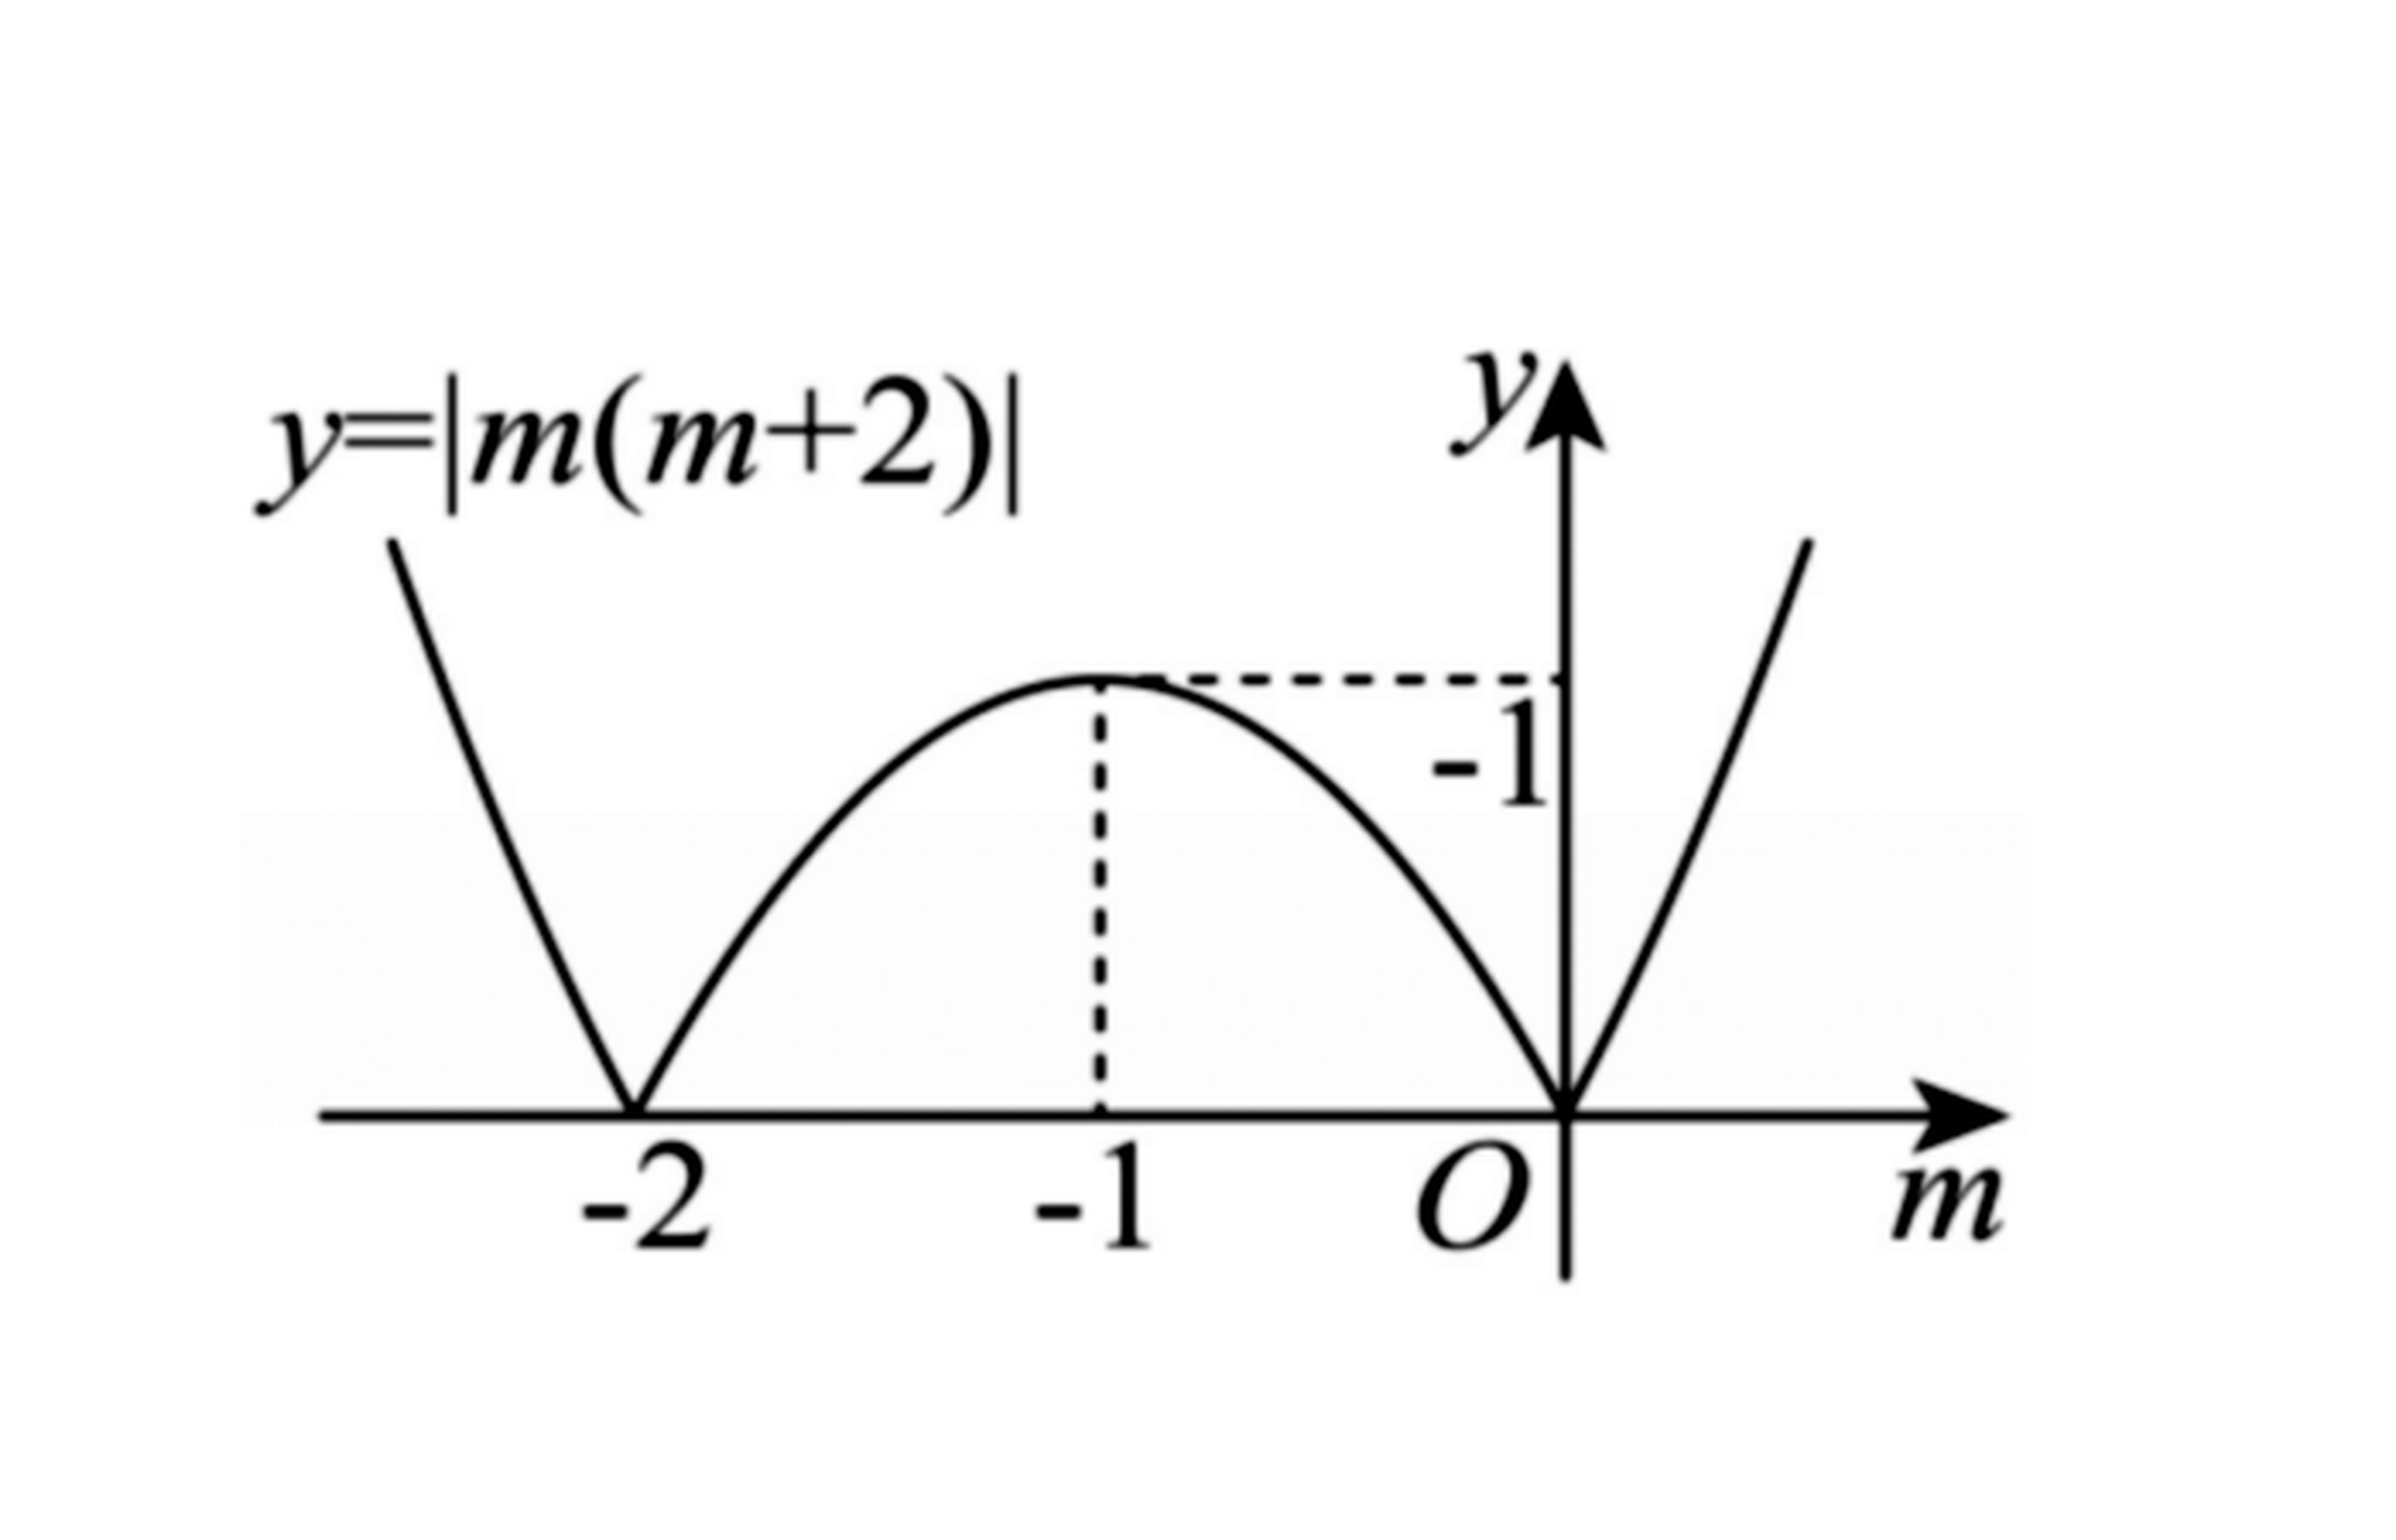
\includegraphics[width=0.46\textwidth]{figures/gao154_fujia2.png}
\end{center}
\step{由图像得 $k\in(0,1)$，}
\step{所以方程 $m^2+2m=k$ 和 $m^2+2m=-k$ 各有两个不同的根，}
\step{其中方程 $m^2+2m-k=0$ 的两根为 $m=-1\pm\sqrt{1+k}$，}
\step{方程 $m^2+2m+k=0$ 的两根为 $m=-1\pm\sqrt{1-k}$，}
\step{所以 $m_1=-1-\sqrt{1+k}$，$m_2=-1-\sqrt{1-k}$，$m_3=-1+\sqrt{1-k}$，$m_4=-1+\sqrt{1+k}$，且 $m_1<m_2<m_3<m_4$，}
\step{由 $m=\log_2 x$，则 $x=2^m$，}
\step{所以 $a=2^{-1-\sqrt{1+k}}$，$b=2^{-1-\sqrt{1-k}}$，$c=2^{-1+\sqrt{1-k}}$，$d=2^{-1+\sqrt{1+k}}$，}
\step{所以 $ad=2^{-1-\sqrt{1+k}}\times2^{-1+\sqrt{1+k}}=2^{(-1-\sqrt{1+k})+(-1+\sqrt{1+k})}=2^{-2}=\dfrac14$，}
\step{$b+c=2^{-1-\sqrt{1-k}}+2^{-1+\sqrt{1-k}}=\dfrac{2^{-\sqrt{1-k}}+2^{\sqrt{1-k}}}{2}$，}
\step{令 $s=\sqrt{1-k}$，其中 $s\in(0,1)$，则 $b+c=\dfrac12\left(2^{-s}+2^s\right)$，}
\step{设函数 $y=2^s+\dfrac1{2^s}$，令 $r=2^s\in(1,2)$，所以 $y=r+\dfrac1r$ 在 $(1,2)$ 上严格增，}
\step{所以函数 $y=2^s+\dfrac1{2^s}$ 在 $(0,1)$ 上严格增，所以 $y=2^s+\dfrac1{2^s}\in\left(2,\dfrac52\right)$，}
\step{所以 $b+c=\dfrac{2^{-s}+2^s}{2}\in\left(1,\dfrac54\right)$，$ad(b+c)=\dfrac{b+c}{4}\in\left(\dfrac14,\dfrac5{16}\right)$，}
\step{所以 $ad(b+c)$ 的取值范围是 $\left(\dfrac14,\dfrac5{16}\right)$，故选 $A$.}
\solend
\fi

\end{enumerate}

\end{document}
"
%
% ① 原始材料：微信公众号"魔都数学加油站"文章，连载"27学年高一154"，原文标题
% "27学年高一154——2026-2027年上海市徐汇中学高一上期中"；
% 原文链接：https://mp.weixin.qq.com/s/Qs2T7Zwsug-KKFE2wefDUg 。
% 正文为 12 张 PNG 页（01/03/04/05/07/11/12 为 2560×3620，
% 02/06/08/09/10 为 4762×6735，同一篇各页分辨率混排，逐页按各自分辨率裁图核对）。
% 体例：讲评版——一、填空题 3—12（10 题）、二、选择题 13—16（4 题）、
% 三、解答题 17—21（5 题）、附加题 1—2（2 题，原卷**另起编号**"1." "2."，
% 不与正题连号，同 高一a 成例），共 21 题；全卷每题均印【解析】
% （逐题核实，见 ② ②）。题目、答案、解析均据原图转录；卷面粉红色水印
% "魔都数学加油站"及公众号页脚未录入。
% 全卷插图清单（逐页通读 12 页确认）：3 组——
%   · Q15 题干配图（$f(x)=(x-a)(x-b)$ 抛物线，04 页右下：x/y 轴、O、1、
%     开口向上两零点均在 (0,1) 内），三版都出，裁 figures/gao154_q15_stem.png；
%   · Q15 四幅图像选项（05 页上半 2×2 排布，A/B/C/D 四幅指数函数图像，
%     合并成一张，照 高一136 Q13/Q22 成例），三版都出，
%     裁 figures/gao154_q15_opts.png；
%   · 附加题第 2 题解析配图（$y=\lvert m(m+2)\rvert$ 图像，11 页右上：
%     W 形折线、$-2$、$-1$、O、虚线 $y=1$ 与 $m=-1$），仅答案版出，
%     裁 figures/gao154_fujia2.png；
%   3 图均取自原卷截图，去粉色水印、去色、4× LANCZOS 放大；Q15 题干图
%   左侧题干残字"的图"已裁白。其余各页逐页确认无其它题目配图、无表格；
%   12 页下半仅水印、无正文。
%
% 卷首标题：原卷印作"2026-2027 年徐汇中学高一上期中"，年份区间按全稿惯例排 en dash；
% 原卷卷面未印副标题，本稿按同期中卷知识模块口径补出"集合与常用逻辑用语、不等式、函数"。
%
% ② 与原卷的排版差异：
%   ① 原文从第 3 题起，本稿保留原题号；共 21 题四节，正题到 21，附加题另起编号
%      1—2（\bigsec{附加题} 后 \begin{enumerate} 不 \setcounter，同 高一a 成例）；
%   ② 全 21 题均印【解析】、用 \solbegin…\solend，无只印【答案】或答案印括号内的题；
%      四道正题选择题答案在解析末句"故选 C／A／B／C"（Q13—Q16）、附加题第 2 题
%      答案在解析末句"故选 A"，括号 \mbox{（\quad）} 留空、不另提 \ans{}；
%      答案版【答案】/【解析】标记数 = 21 = 全卷题数；
%   ③ 原卷卷面未印副标题，本稿按知识模块口径补出；
%   ④ 原卷填空横线按全稿惯例排 \blankline[4.4em]；选择题括号排 \mbox{（\quad）}、
%      四道正题选择题与附加题第 2 题的选项段前按惯例各加 \keepwithprev
%      （Q15 与附加题 2 的选项段是整块图，\keepwithprev 后接 \begin{center}）；
%      解答题不留作答区、不加 \anspace（原卷为讲评版）；
%   ⑤ 数集黑板粗体：Q4"$x,y\in R$"、Q9"$x\in\R$"、Q13 无、
%      Q15"定义域 $\R$"、Q19"$\forall x\in\R$"、Q21"$x\in\N$"与"$k\in\N^*$"、
%      Q20"$a,b\in\R$"、附加题 2 无——原卷印斜体或正体粗体 R/N/N*，
%      按全稿惯例归一 \R／\N／\N^*；绝对值排 \lvert…\rvert
%      （Q5、Q9、Q12、Q13、Q16、Q21、附加题 2），集合描述竖线排 \mid
%      （Q5、Q17、Q19、Q21），不等号按全稿惯例排 \leqslant／\geqslant；
%      空集 \varnothing（Q21 题干 (3)）；
%   ⑥ 子集符号逐处照录、不得统一：Q6 题干印"$\{1,2\}\subset M\subseteq\{1,2,3,4,5\}$"
%      （前单线 ⊂、后带下划线 ⊆，同句两形并用），解析亦两形并用；
%      Q17 解析 (2)"$B\subset A$"印单线 ⊂；Q21 题干 (3)"$A\subseteq\{x\mid\cdots\}$"
%      印带下划线 ⊆——逐处放大核，分别 \subset／\subseteq，照录未统一（见 ④）；
%   ⑦ 判别式 Δ/△：Q18 解析 (1)"$\Delta=m^2-4(4m^2-3)$"与 Q19 解析 (1)
%      "$\Delta=4m^2-8m<0$"两处均印等腰偏高粗三角、照录 \Delta；本卷无扁等边
%      细线 \triangle 用例（见 ④）；
%   ⑧ 中文弯引号照录：Q4"设 $x$、$y\in\R$. 若 $x+y>2$，则 $x>1$ 或 $y>1$"、
%      附加题 1"$n$ 元集和集"与"3 元集和集"；注释里一律 ASCII 引号；
%      数学式内 CJK 用 \text{}（Q5 解集描述"或"、Q19 集合描述的"或"）；
%   ⑨ "图像／图象"逐处放大核：Q15 题干与解析印"图象"（象，无亻）、
%      Q16 无、附加题 2 解析印"图象"与"图像"（"画出函数…的图象"、
%      "由图像得"——两形并用，逐处照录未统一）；Q13/Q14 无数集图像字样；
%      半角逗号在数学组之间是全稿惯例、非笔误，逐处照录（Q3、Q10、Q16、
%      Q18、Q20、Q21 的 $x_1,x_2$ 之类）；行末西文句点 ASCII `.`；
%      行中全角逗号／顿号照录（Q6"3，4，5"、Q20"（单位：元）"、
%      附加题 1"$a_1,a_2,a_3,a_4$"）；
%   ⑩ 复杂式照录别简化：Q3 $a^{\frac{12}{7}}\cdot\left(\frac17\right)^{\frac17}
%      \cdot\sqrt[7]{a^4}$ 与 $7^{-\frac17}a^{\frac{16}{7}}$、Q7 $x^{-m}$、
%      Q8 $\frac{b-2a+2}{2a}$、Q11 $\frac{9+4\sqrt2}{6}$、Q12 $506\frac29$ 与
%      $506\frac49$、Q16 高斯取整 $[a]$、Q20 $c(x)=10x+\frac1{100}x^2$ 与
%      $q(x)=a+\frac xb$、Q21 $A^+$／$A^-$ 与 $|A^+|\geqslant2k-1$、
%      附加题 2 $m=-1\pm\sqrt{1+k}$ 与 $ad(b+c)$；
%      \left…\right 不得拆到不同 $…$ 组（Q5 $\left\{x\mid\cdots\right\}$、
%      Q20 $\left(\frac1b-\frac1{100}\right)$、附加题 2 $\left(\frac14,\frac5{16}\right)$）；
%      cases 块一律 \begin{cases}…\end{cases}；
%   ⑪ 一条 \step = 原卷解析的一个印刷行，cases 块整体算一个印刷行；别并折行、
%      别拆行。Q11 九行、Q12 六行、Q16 十六行、Q20 十一行、Q21 十七行、
%      附加题 2 十八行均按印刷行逐条断，不丢行；
%   ⑫ 配图：Q15 题干小图（三版都出）放 \item 内题干之后 \begin{center}，
%      Q15 四幅选项图（三版都出）放 \keepwithprev 之后的 \begin{center}，
%      Q15 用 \needvspace 守卫把"题干＋两图"整块推走（守卫放 \item 之前，
%      见 高一145 Q14/Q20 与 高一136 Q13 成例）；附加题 2 解析配图（仅答案版出）
%      放 \ifanswer 内 \solbegin…\solend 的 \step 之间（高一73 第 16 题成例）；
%   ⑬ 原卷解析内无红色"法一／法二"之类小标题，故本卷无 \stepm；红色水印
%      "魔都数学加油站"不录入；
%   ⑭ 跨页续印按题合并：见 ⑥；
%
% ③ 行数复核：一条 \step = 原卷解析的一个印刷行，cases 块作一个印刷行计。
%   逐题数（主会话逐页核对定稿）：Q3：1；Q4：1；Q5：3；Q6：4；Q7：3；
%   Q8：1；Q9：5；Q10：4；Q11：9；Q12：6；Q13：5；Q14：4；Q15：3；
%   Q16：16；Q17：5；Q18：9；Q19：10；Q20：11；Q21：17；
%   附加题 1：6；附加题 2：18。
%   合计 141 条 \step（本卷无 \stepm），与原卷逐题印刷行相等。全卷 21 题
%   均设 \solbegin…\solend，答案版【答案】/【解析】标记数 = 21 = 全卷题数。
%
% ④ 判别式／子集符号结论（逐处放大原图照录、不得统一，主会话像素级复核）：
%   判别式：Q18 解析 (1)"$\Delta=m^2-4(4m^2-3)=-15m^2+12\geqslant0$"、
%      Q19 解析 (1)"$\Delta=4m^2-8m<0$"共 2 处，逐处放大确认印等腰偏高
%      粗三角（高>宽、右斜边粗），照录 \Delta；本卷无扁等边细线 \triangle
%      用例，无几何三角形符号。
%   子集：Q6 题干"$\{1,2\}\subset M\subseteq\{1,2,3,4,5\}$"前 ⊂ 单线、
%      后 ⊆ 带下划线（/tmp/gao154/z/zoom/q6_subset.png），解析两处同样两形
%      并用，分别照录 \subset／\subseteq；Q17 解析 (2)"$B\subset A$"单线
%      照录 \subset；Q21 题干 (3)"$A\subseteq\{x\mid\cdots\}$"带下划线
%      照录 \subseteq。本卷 ⊂ 与 ⊆ 混用逐处照录、不得统一。
%      空集 \varnothing（Q21 题干 (3)）、数集 \R／\N／\N^* 归一见 ② ⑤。
%
% ⑤ 存疑照录（放大原图确认，照录未改、正文对应处另有 % 注）：
%   1. Q7 题干印 $f(x)=(3m-1)x^{-m}$，解析首句却写"幂函数 $f(x)=x^\alpha$
%      的系数必须为 1"（用 $\alpha$ 作指数记号），随后 $f(2)=2^\alpha=8$
%      得 $\alpha=3$、$f(x)=x^3$——题干指数 $-m$ 与解析 $\alpha$ 记法不同，
%      系原卷记号前后不一，逐处照录未统一（放大 01/02 页确认）。
%   2. Q11 解析"因为 $u>0,v>0$，由基本不等式得 $\frac{4v}{u}+\frac{2u}{v}
%      \geqslant2\sqrt{\frac{4v}{u}\cdot\frac{2u}{v}}=4\sqrt2$"与
%      "所以 $\frac4u+\frac1v=\frac16\left(\frac4u+\frac1v\right)(2u+v)$"
%      照录，未把 $u,v$ 化简回 $x,y$。
%   3. Q16 解析把"$[a]$ 表示不超过 $a$ 的最大整数"与"和至少有一个不小于 2"
%      连写在同一行（原卷如此），照录未改；末行"假设成立，C 正确，D 错误"照录。
%   4. Q18 解析 (2)"函数 $y=-7m^2+6$ 开口向下，对称轴为 $m=0$"却称求
%      "$y_{\min}$"（实为在 $m^2\leqslant\frac45$ 闭区间上的最小值），
%      照录未改。
%   5. Q20 题干"$q(x)=a+\frac xb$（$a,b\in\R$）"与解析
%      "$W(x)=\left(\frac1b-\frac1{100}\right)x^2+(a-10)x-160000$"照录；
%      末行解得 $a=90,b=\frac{500}{3}$ 照录未化简。
%   6. Q21 题干 (3)"$A\subseteq\{x\mid0\leqslant x\leqslant2020,x\in\N\}$"
%      与解析"$3k-1\leqslant2a_k+1\leqslant4041$（$k\in\N^*$）"照录；
%      末行"集合 $A$ 中元素的个数的最大值是 1347"照录。
%   7. 附加题 1 解析"相加化简得 $a_1+a_2+a_3+a_4=5$"照录；
%      附加题 2 解析"由图像得 $k\in(0,1)$"与"由图像得"／"的图象"两形
%      并用逐处照录（见 ② ⑨）；末行"$ad(b+c)$ 的取值范围是
%      $\left(\frac14,\frac5{16}\right)$，故选 A"照录。
%   全卷除此 7 类外未发现其它笔误／自相矛盾处；21 题均印【解析】、
%   无只印【答案】或答案印括号内的题（见 ② ②）。
%
% ⑥ 跨页续印按题合并说明（逐页核实定稿）：Q3—Q5 题干＋解析在 01 页
%   （Q5 解析末 2 行续 01 页下半）；Q6、Q7 题干＋解析在 01 页下半
%   （Q7 解析余 2 行续 02 页顶）；Q8、Q9 题干＋解析在 02 页上半
%   （Q9 解析余 3 行续 02 页下半）；Q10 题干＋解析在 02 页下半；
%   Q11 题干＋解析前 6 行在 03 页上半、余 3 行续 03 页下半；
%   Q12 题干＋解析前 5 行在 03 页下半、末行续 04 页顶；"二、选择题"
%   标题与 Q13 题干＋选项＋解析在 04 页上半；Q14 题干＋选项＋解析、
%   Q15 题干＋题干配图在 04 页下半；Q15 四幅选项图＋解析、
%   Q16 题干＋选项＋解析首行在 05 页上半，Q16 解析余 12 行在
%   05 页下半—06 页上半；"三、解答题"标题与 Q17 题干＋两问＋解析
%   在 06 页下半；Q18 题干＋两问＋解析在 07 页上半—下半；
%   Q19 题干＋两问＋解析首行在 07 页下半，解析余 8 行在 08 页上半；
%   Q20 题干在 08 页下半，解析 (1) 4 行＋(2) 首 4 行在 08 页下半—09 页上半，
%   (2) 余 2 行在 09 页下半；Q21 题干＋三问＋解析 (1)(2) 4 行在
%   09 页下半—10 页上半，解析 (3) 余 12 行在 10 页上半—下半；
%   "附加题"标题与附加题 1 题干＋解析首 3 行在 10 页下半，
%   余 3 行续 11 页上半；附加题 2 题干＋选项＋解析前 3 行在 11 页上半，
%   解析配图＋余 12 行在 11 页下半—12 页上半，末行
%   "所以 $ad(b+c)$ 的取值范围是 $\left(\frac14,\frac5{16}\right)$，故选 A"
%   为全卷收尾（12 页下半仅水印、无正文）。
%   本稿按题连排，不丢行、不并折行；全卷末题为附加题第 2 题。
%
\documentclass[a4paper,11pt]{article}
\usepackage{common}

\begin{document}

\examtitlest[3]{2026--2027 年徐汇中学高一上期中}{集合与常用逻辑用语、不等式、函数}

\bigsec{一、填空题}

\begin{enumerate}
\setcounter{enumi}{2}

% === Q3 === 分数指数幂照录；解析 1 行
\item 已知 $a>0$，化简 $a^{\frac{12}{7}}\cdot\left(\dfrac17\right)^{\frac17}\cdot\sqrt[7]{a^4}=$\blankline[4.4em].

\ifanswer
\solbegin
\step{$a^{\frac{12}{7}}\cdot\left(\dfrac17\right)^{\frac17}\cdot\sqrt[7]{a^4}=a^{\frac{12}{7}}\cdot(7^{-1})^{\frac17}\cdot a^{\frac47}=7^{-\frac17}a^{\frac{16}{7}}$.}
\solend
\fi

% === Q4 === 反证法；中文弯引号照录；解析 1 行
\item 用反证法证明命题：“设 $x$、$y\in\R$. 若 $x+y>2$，则 $x>1$ 或 $y>1$”时，假设的内容应该是\blankline[4.4em].

\ifanswer
\solbegin
\step{由反证法得，假设的内容应该是 $x\leqslant1$ 且 $y\leqslant1$.}
\solend
\fi

% === Q5 === 分式不等式；cases 块；解析 3 行
\item 不等式 $\dfrac{2x+3}{x-1}\geqslant1$ 的解集为\blankline[4.4em].

\ifanswer
\solbegin
\step{$\dfrac{2x+3}{x-1}\geqslant1$，即 $\dfrac{2x+3}{x-1}-1\geqslant0$，$\dfrac{x+4}{x-1}\geqslant0$，}
\step{等价于 $\begin{cases}(x+4)(x-1)\geqslant0\\x-1\ne0\end{cases}$，解得 $x>1$ 或 $x\leqslant-4$，}
\step{故解集为 $\{x\mid x>1\text{ 或 }x\leqslant-4\}$.}
\solend
\fi

% === Q6 === ⊂ 与 ⊆ 并用照录；解析 4 行
\item 满足条件 $\{1,2\}\subset M\subseteq\{1,2,3,4,5\}$ 的集合 $M$ 的个数为\blankline[4.4em].

\ifanswer
\solbegin
\step{因为 $\{1,2\}\subset M\subseteq\{1,2,3,4,5\}$，所以集合 $M$ 必含有元素 1，2，}
\step{且至少含有元素 3，4，5 中的一个，}
\step{则集合 $M$ 的个数与集合 $\{3,4,5\}$ 的非空子集的个数一样，}
\step{所以集合 $M$ 的个数为 $2^3-1=7$.}
\solend
\fi

% === Q7 === 题干 $x^{-m}$、解析用 $x^\alpha$ 记法，原卷记号差异照录（见 ⑤ 1）；解析 3 行
\item 已知幂函数 $f(x)=(3m-1)x^{-m}$，且 $f(2)=8$，则 $f(m)=$\blankline[4.4em].

\ifanswer
\solbegin
\step{幂函数 $f(x)=x^\alpha$ 的系数必须为 1，所以 $3m-1=1$，得 $m=\dfrac23$.}
\step{又 $f(2)=2^\alpha=8=2^3$，故 $\alpha=3$，即 $f(x)=x^3$，}
\step{所以 $f(m)=f\left(\dfrac23\right)=\left(\dfrac23\right)^3=\dfrac8{27}$.}
\solend
\fi

% === Q8 === 换底公式；解析 1 行
\item 已知 $a=\lg2$，$b=\lg3$，用含 $a,b$ 的代数式表示 $\log_4 75=$\blankline[4.4em].

\ifanswer
\solbegin
\step{$\log_4 75=\dfrac{\lg\left(3\times\frac{10^2}{2^2}\right)}{\lg2^2}=\dfrac{\lg3+2-2\lg2}{2\lg2}=\dfrac{b-2a+2}{2a}$.}
\solend
\fi

% === Q9 === 三角不等式取等；解析 5 行
\item 设 $x\in\R$，则方程 $\lvert x-2\rvert+\lvert3x+1\rvert=\lvert2x+3\rvert$ 的解集是\blankline[4.4em].

\ifanswer
\solbegin
\step{由 $\lvert x-2\rvert=\lvert2-x\rvert$，故原方程可化为 $\lvert2-x\rvert+\lvert3x+1\rvert=\lvert2x+3\rvert$，}
\step{又 $(2-x)+(3x+1)=2x+3$，}
\step{由三角不等式 $\lvert2-x\rvert+\lvert3x+1\rvert\geqslant\lvert(2-x)+(3x+1)\rvert=\lvert2x+3\rvert$，}
\step{当且仅当 $(2-x)(3x+1)\geqslant0$ 等号成立，}
\step{解 $(2-x)(3x+1)\geqslant0$ 得 $-\dfrac13\leqslant x\leqslant2$，故原方程的解集为 $\left[-\dfrac13,2\right]$.}
\solend
\fi

% === Q10 === 韦达定理；cases 块；解析 4 行
\item 已知一元二次不等式 $x^2+bx+c>0$ 的解集为 $(-\infty,-1)\cup(2,+\infty)$，则一元二次不等式 $bx^2+cx-1<0$ 的解集是\blankline[4.4em].

\ifanswer
\solbegin
\step{因为 $x^2+bx+c>0$ 的解集为 $(-\infty,-1)\cup(2,+\infty)$，}
\step{所以方程 $x^2+bx+c=0$ 的两根为 $-1$ 和 2，则有 $\begin{cases}-b=-1+2\\c=-1\times2\end{cases}$，即 $\begin{cases}b=-1\\c=-2\end{cases}$，}
\step{则 $bx^2+cx-1<0$ 等价于 $-x^2-2x-1<0$，得 $x^2+2x+1>0$，得 $(x+1)^2>0$，}
\step{解得 $x\ne-1$，故不等式 $bx^2+cx-1<0$ 的解集为 $(-\infty,-1)\cup(-1,+\infty)$.}
\solend
\fi

% === Q11 === 换元 $u,v$；解析 9 行
\item 已知正数 $x,y$ 满足 $2x+y=1$，则 $\dfrac4{x+2}+\dfrac1{y+1}$ 的最小值为\blankline[4.4em].

\ifanswer
\solbegin
\step{令 $u=x+2$，$v=y+1$，则 $u>2$，$v>1$，}
\step{且 $2u+v=2(x+2)+(y+1)=2x+y+5=6$.}
\step{因为 $u>0$，$v>0$，由基本不等式得 $\dfrac{4v}{u}+\dfrac{2u}{v}\geqslant2\sqrt{\dfrac{4v}{u}\cdot\dfrac{2u}{v}}=4\sqrt2$，}
\step{所以 $\dfrac4u+\dfrac1v=\dfrac16\left(\dfrac4u+\dfrac1v\right)(2u+v)=\dfrac16\left(9+\dfrac{4v}{u}+\dfrac{2u}{v}\right)\geqslant\dfrac{9+4\sqrt2}{6}$，}
\step{当且仅当 $\dfrac{4v}{u}=\dfrac{2u}{v}$，即 $u=\sqrt2v$ 时等号成立，}
\step{与 $2u+v=6$ 联立得 $u=\dfrac{6\sqrt2}{2\sqrt2+1}$，$v=\dfrac6{2\sqrt2+1}$，}
\step{此时 $x=u-2=\dfrac{2\sqrt2-2}{2\sqrt2+1}>0$，$y=v-1=\dfrac{5-2\sqrt2}{2\sqrt2+1}>0$，且 $2x+y=1$，}
\step{满足题设，所以下界可以取得，}
\step{因此 $\dfrac4{x+2}+\dfrac1{y+1}$ 的最小值为 $\dfrac{9+4\sqrt2}{6}$.}
\solend
\fi

% === Q12 === 2025 个整数解；解析 6 行
\item 若关于 $x$ 的不等式 $\lvert x-2k\rvert+\lvert x-3k\rvert<4k$ 共有 2025 个整数解，则实数 $k$ 的取值范围为\blankline[4.4em].

\ifanswer
\solbegin
\step{显然 $k>0$，由 $\lvert x-2k\rvert+\lvert x-3k\rvert<4k$，得 $\dfrac12k<x<\dfrac92k$，}
\step{因为该不等式共有 2025 个整数解，所以 $2024<\dfrac{9k}{2}-\dfrac k2\leqslant2026$，}
\step{解得 $506<k\leqslant506.5$，}
\step{由 $\dfrac k2\in(253,253.25]$，得这 2025 个整数解只能为 254、255、256、$\cdots$、2278，}
\step{所以 $2278<\dfrac{9k}{2}\leqslant2279$，解得 $506\dfrac29<k\leqslant506\dfrac49$，结合 $506<k\leqslant506.5$，}
\step{得 $k$ 的取值范围是 $\left(506\dfrac29,506\dfrac49\right]$.}
\solend
\fi

\end{enumerate}

\bigsec{二、选择题}

\begin{enumerate}
\setcounter{enumi}{12}

% === Q13 === 四选项一行；解析 5 行，故选 C
\item 若 $a<b<0$，则下列不等式中不成立的是\mbox{（\quad）}

\keepwithprev
A. $a-b>a$\qquad B. $\dfrac1a>\dfrac1b$\qquad C. $a^3>b^3$\qquad D. $\lvert a\rvert>\lvert b\rvert$

\ifanswer
\solbegin
\step{A 选项，因为 $b<0$，所以 $-b>0$，不等式两边同加上 $a$ 得 $a-b>a$，故 A 正确；}
\step{B 选项，因为 $a<b<0$，所以 $ab>0$，不等式两边同除以 $ab$，则 $\dfrac1b<\dfrac1a<0$，故 B 正确；}
\step{C 选项，不妨设 $a=-2$，$b=-1$，则 $a^3=-8$，$b^3=-1$，故 $a^3<b^3$，故 C 错误；}
\step{D 选项，因为 $a<b<0$，所以 $-a>-b$，即 $\lvert a\rvert>\lvert b\rvert$，故 D 正确.}
\step{故选 $C$.}
\solend
\fi

% === Q14 === 选项两行两列；解析 4 行，故选 A
\item 设命题 $p:x^2-5x+4\ne0$，命题 $q:x\ne1$，则 $p$ 是 $q$ 的\mbox{（\quad）}条件

\keepwithprev
A. 充分不必要\qquad\qquad B. 必要不充分

C. 充要\qquad\qquad D. 既不充分也不必要

\ifanswer
\solbegin
\step{$p:x^2-5x+4\ne0\Leftrightarrow(x-1)(x-4)\ne0\Leftrightarrow x\ne1$ 且 $x\ne4$；$q:x\ne1$.}
\step{充分性：当 $x\ne1$ 且 $x\ne4$ 时，$x\ne1$，所以 $p\Rightarrow q$；}
\step{必要性：当 $x\ne1$ 时，若 $x=4$，此时 $p$ 不成立，即 $q\nRightarrow p$；}
\step{所以 $p$ 是 $q$ 的充分不必要条件，故选 $A$.}
\solend
\fi

% === Q15 === 题干配图（三版都出）+ 四幅图像选项（2×2 合并，三版都出）；守卫放 \item 之前；解析 3 行，故选 B
\needvspace{9cm}
\item 已知函数 $f(x)=(x-a)(x-b)$（$a<b$）的图象如图所示，则函数 $g(x)=a^x-b$ 的图象可能是\mbox{（\quad）}

\begin{center}
% 抛物线题干配图取 04 页右下，去粉色水印、去色、4× LANCZOS 放大；三版都出
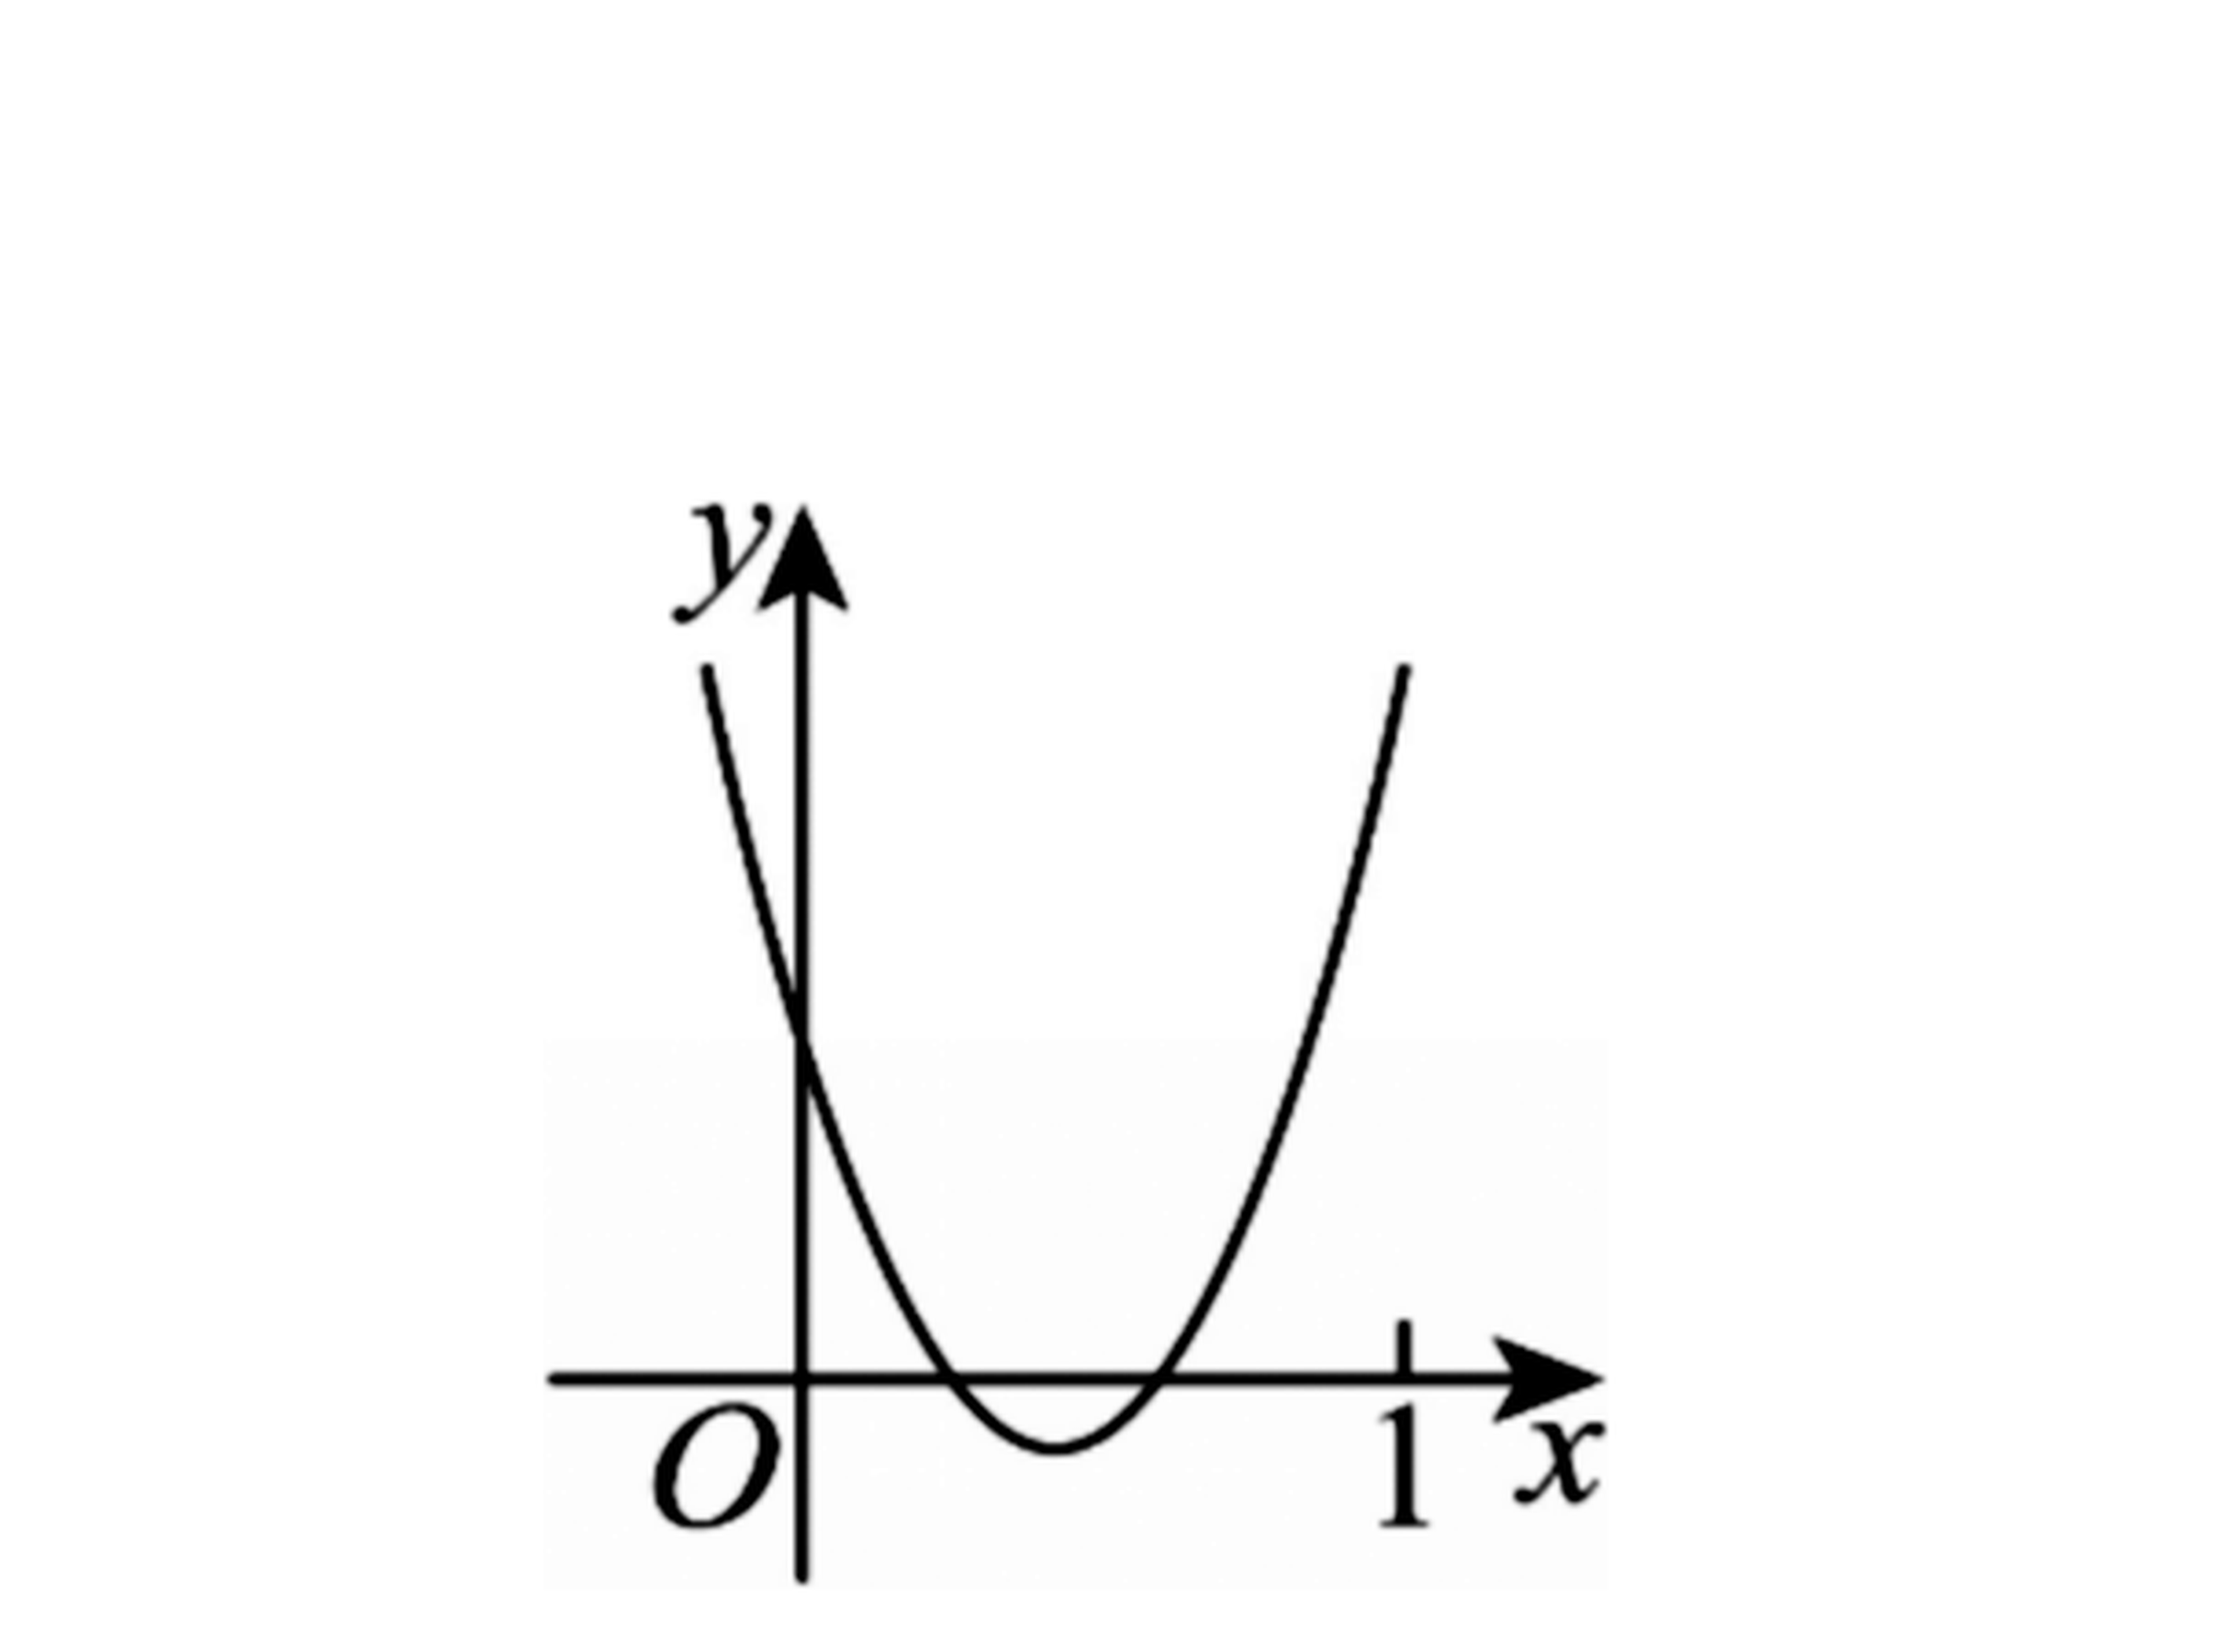
\includegraphics[width=0.32\textwidth]{figures/gao154_q15_stem.png}
\end{center}

\keepwithprev
\begin{center}
% 四幅指数函数图像选项取 05 页上半，按原卷 2×2 排布合并为一张，去粉色水印、去色、4× LANCZOS 放大；三版都出
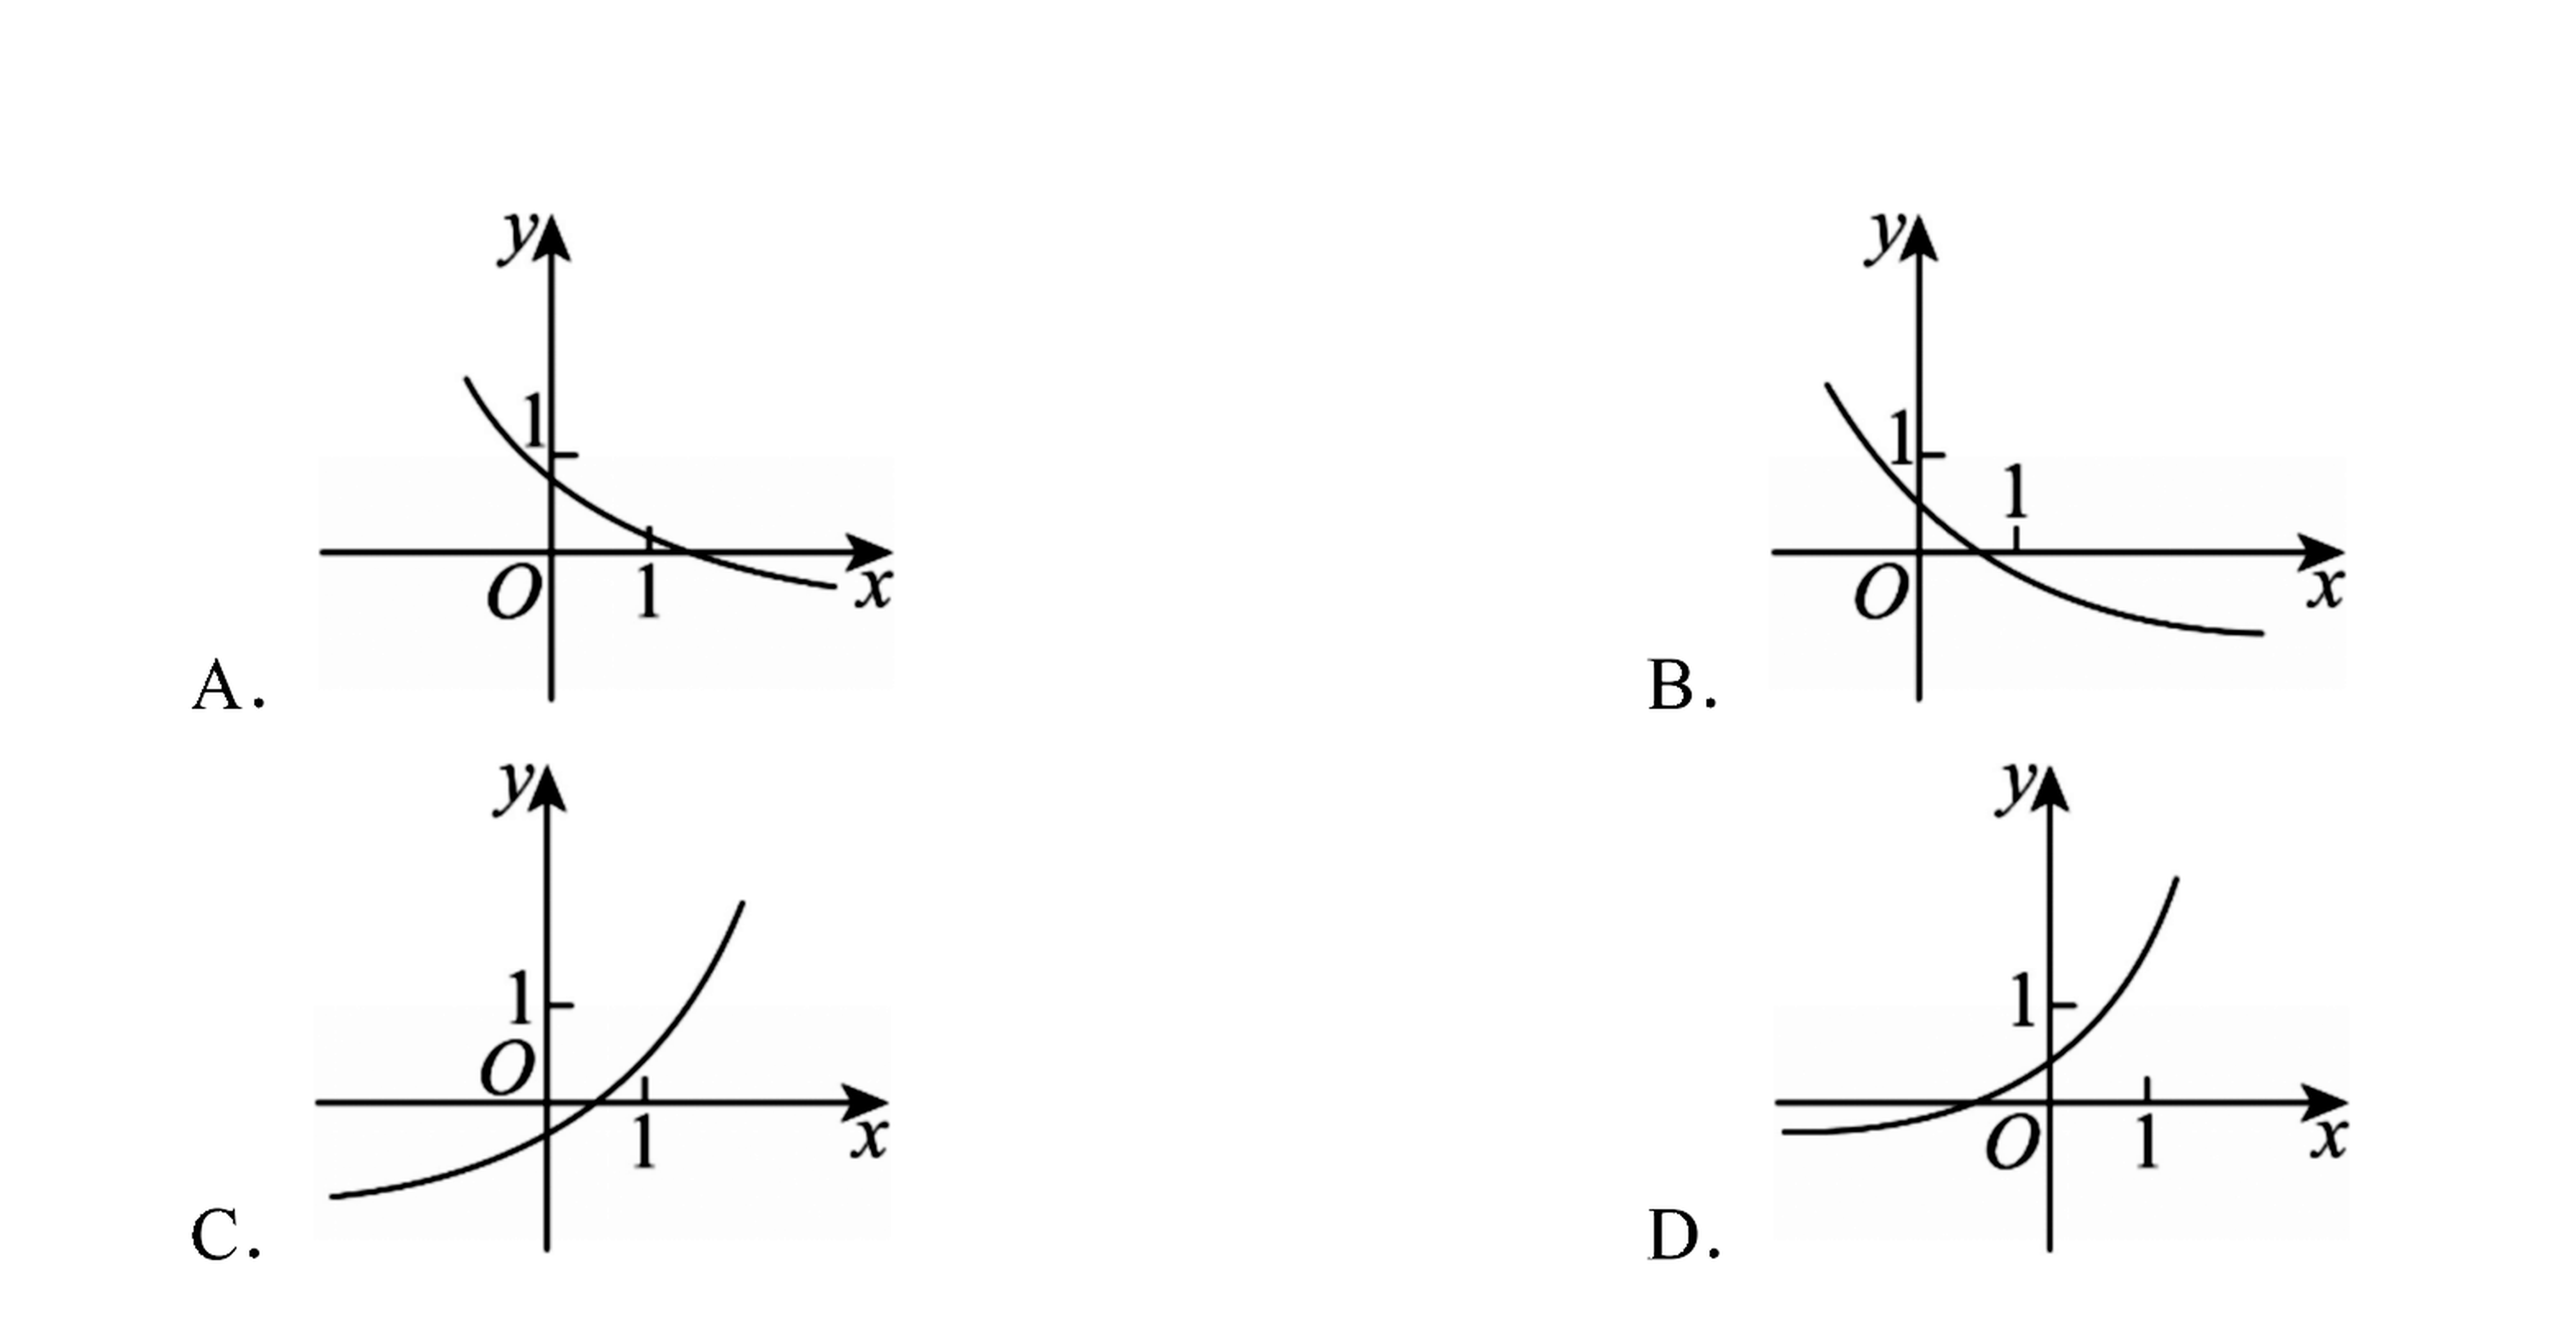
\includegraphics[width=0.80\textwidth]{figures/gao154_q15_opts.png}
\end{center}

\ifanswer
\solbegin
\step{由题意得 $0<a<b<1$，所以 $g(x)=a^x-b$ 在定义域 $\R$ 上严格减.}
\step{$g(0)=a^0-b=1-b>0$，$g(1)=a^1-b=a-b<0$，故 B 符合题意.}
\step{故选 $B$.}
\solend
\fi

% === Q16 === 高斯取整；解析 13 行，故选 C
\item 设 $[a]$ 表示不超过 $a$ 的最大整数，如 $[1.2]=1$，$[-3.2]=-4$，若 $x$、$y$、$z$ 为正实数，则 $\left[\dfrac{y+z}{x}\right]+\left[\dfrac{z+x}{y}\right]+\left[\dfrac{x+y}{z}\right]$ 的最小值为\mbox{（\quad）}

\keepwithprev
A. 2\qquad\qquad B. 3\qquad\qquad C. 4\qquad\qquad D. 6

\ifanswer
\solbegin
\step{若 $x$、$y$、$z$ 为正实数，}
\step{结合基本不等式得 $\dfrac{y+z}{x}+\dfrac{z+x}{y}+\dfrac{x+y}{z}=\dfrac yx+\dfrac xy+\dfrac zx+\dfrac xz+\dfrac zy+\dfrac yz$}
\step{$\geqslant2\sqrt{\dfrac yx\cdot\dfrac xy}+2\sqrt{\dfrac zx\cdot\dfrac xz}+2\sqrt{\dfrac zy\cdot\dfrac yz}=6$，当且仅当 $x=y=z$ 时取等号，}
\step{即 $\dfrac{y+z}{x}$，$\dfrac{z+x}{y}$，$\dfrac{x+y}{z}$ 中至少有一个不小于 2，不妨设 $\dfrac{y+z}{x}\geqslant\dfrac{z+x}{y}\geqslant\dfrac{x+y}{z}$，}
\step{$[a]$ 表示不超过 $a$ 的最大整数和 $\dfrac{y+z}{x}$，$\dfrac{z+x}{y}$，$\dfrac{x+y}{z}$ 中至少有一个不小于 2，}% 原卷此行把两句连写，照录未改（见 ⑤ 3）
\step{得 $\left[\dfrac{y+z}{x}\right]\geqslant2$，所以 $\left[\dfrac{y+z}{x}\right]+\left[\dfrac{z+x}{y}\right]+\left[\dfrac{x+y}{z}\right]\geqslant2$，}
\step{假设 $\left[\dfrac{y+z}{x}\right]+\left[\dfrac{z+x}{y}\right]+\left[\dfrac{x+y}{z}\right]$ 的最小值为 2，$\left[\dfrac{y+z}{x}\right]=2$，$\left[\dfrac{z+x}{y}\right]+\left[\dfrac{x+y}{z}\right]=0$，}
\step{所以 $2\leqslant\dfrac{y+z}{x}<3$，$0<\dfrac{z+x}{y}<1$，$0<\dfrac{x+y}{z}<1$，所以 $2<\dfrac{y+z}{x}+\dfrac{z+x}{y}+\dfrac{x+y}{z}<5$，}
\step{与 $\dfrac{y+z}{x}+\dfrac{z+x}{y}+\dfrac{x+y}{z}\geqslant6$ 矛盾，假设不成立，A 错误；}
\step{假设 $\left[\dfrac{y+z}{x}\right]+\left[\dfrac{z+x}{y}\right]+\left[\dfrac{x+y}{z}\right]$ 的最小值为 3，}
\step{则 $\left[\dfrac{y+z}{x}\right]=2$，$\left[\dfrac{z+x}{y}\right]=1$，$\left[\dfrac{x+y}{z}\right]=0$ 或 $\left[\dfrac{y+z}{x}\right]=3$，$\left[\dfrac{z+x}{y}\right]=\left[\dfrac{x+y}{z}\right]=0$，}
\step{同理可得 $3<\dfrac{y+z}{x}+\dfrac{z+x}{y}+\dfrac{x+y}{z}<6$，显然不成立，B 错误；}
\step{假设 $\left[\dfrac{y+z}{x}\right]+\left[\dfrac{z+x}{y}\right]+\left[\dfrac{x+y}{z}\right]$ 的最小值为 4，易得 $4<\dfrac{y+z}{x}+\dfrac{z+x}{y}+\dfrac{x+y}{z}<7$，}
\step{若取 $x=100$，$y=103$，$z=104$，则 $\left[\dfrac{y+z}{x}\right]=2$，$\left[\dfrac{z+x}{y}\right]=1$，$\left[\dfrac{x+y}{z}\right]=1$，}
\step{即 $\left[\dfrac{y+z}{x}\right]+\left[\dfrac{z+x}{y}\right]+\left[\dfrac{x+y}{z}\right]=4$，假设成立，C 正确，D 错误.}
\step{故选 $C$.}
\solend
\fi

\end{enumerate}

\bigsec{三、解答题}

\begin{enumerate}
\setcounter{enumi}{16}

% === Q17 === $B\subset A$ 单线照录；cases 块；解析 5 行
\item 设集合 $A=\{x\mid x^2+2x-3<0\}$，集合 $B=\{x\mid\lvert x+a\rvert<1\}$.

(1) 若 $a=3$，求 $A\cup B$；

(2) 设命题 $p:x\in A$，命题 $q:x\in B$，若 $p$ 是 $q$ 成立的必要不充分条件，求实数 $a$ 的取值范围.

\ifanswer
\solbegin
\step{(1) $A=(-3,1)$，}
\step{当 $a=3$ 时，$\lvert x+3\rvert<1$，解得 $-4<x<-2$，所以 $B=(-4,-2)$，}
\step{所以 $A\cup B=(-4,1)$.}
\step{(2) 因为 $p$ 是 $q$ 成立的必要不充分条件，所以 $B\subset A$.}
\step{因为 $A=(-3,1)$，$B=(-a-1,-a+1)$，所以 $\begin{cases}-a-1\geqslant-3\\-a+1<1\end{cases}$ 或 $\begin{cases}-a-1>-3\\-a+1\leqslant1\end{cases}$，解得 $0\leqslant a\leqslant2$.}
\solend
\fi

% === Q18 === 判别式 \Delta 两处照录；解析 9 行
\item 已知关于 $x$ 的一元二次方程 $x^2-mx+4m^2-3=0$ 的两个实根分别为 $x_1,x_2$.

(1) 若 $x_1,x_2$ 满足 $x_1+x_2=x_1x_2$，求实数 $m$ 的值；

(2) 求 $x_1^2+x_2^2$ 的最小值.

\ifanswer
\solbegin
\step{(1) 由韦达定理 $x_1+x_2=m$，$x_1x_2=4m^2-3$，}
\step{$\Delta=m^2-4(4m^2-3)=-15m^2+12\geqslant0$，即 $m^2\leqslant\dfrac45$.}
\step{由 $x_1+x_2=x_1x_2$ 得 $m=4m^2-3$，即 $4m^2-m-3=0$，}
\step{解得 $m=1$ 或 $m=-\dfrac34$.}
\step{$m=1$ 时 $m^2=1>\dfrac45$，$\Delta<0$，舍去；}
\step{$m=-\dfrac34$ 时 $m^2=\dfrac9{16}<\dfrac45$，符合，故 $m=-\dfrac34$.}
\step{(2) $x_1^2+x_2^2=(x_1+x_2)^2-2x_1x_2=m^2-2(4m^2-3)=-7m^2+6$，}
\step{函数 $y=-7m^2+6$ 开口向下，对称轴为 $m=0$，}% 原卷此处称求「最小值」，实为闭区间 $m^2\le\frac45$ 上的最小值，照录未改（见 ⑤ 4）
\step{故 $y_{\min}=-7\cdot\dfrac45+6=-\dfrac{28}{5}+\dfrac{30}{5}=\dfrac25$.}
\solend
\fi

% === Q19 === 全称命题；cases 块；解析 9 行
\item 设命题 $p$：对任意 $x\in\R$，不等式 $2mx^2+2mx+1>0$ 恒成立，$q:m\in\{m\mid\log_2(m-1)<1\}$.

(1) 若 $p$ 为真命题，求实数 $m$ 的取值范围；

(2) 若命题 $p$、$q$ 有且只有一个是真命题，求实数 $m$ 的取值范围.

\ifanswer
\solbegin
\step{(1) 由 $p$ 为真命题，得 $\forall x\in\R$，不等式 $2mx^2+2mx+1>0$ 恒成立，}
\step{当 $m=0$ 时，$1>0$ 恒成立；}
\step{当 $m\ne0$ 时，$\begin{cases}2m>0\\\Delta=4m^2-8m<0\end{cases}$，解得 $0<m<2$；}
\step{综上，$0\leqslant m<2$，即 $m$ 的取值范围是 $[0,2)$；}
\step{(2) 若 $q$ 为真，则有 $\log_2(m-1)<1$，得 $0<m-1<2$，解得 $1<m<3$，}
\step{因此命题 $q:m\in\{m\mid1<m<3\}$，由 (1) 得命题 $p:\{m\mid0\leqslant m<2\}$，}
\step{而命题 $p$、$q$ 有且只有一个是真命题，}
\step{当 $p$ 真 $q$ 假时，$\begin{cases}0\leqslant m<2\\m\leqslant1\text{ 或 }m\geqslant3\end{cases}$，解得 $0\leqslant m\leqslant1$，}
\step{当 $p$ 假 $q$ 真时，$\begin{cases}m<0\text{ 或 }m\geqslant2\\1<m<3\end{cases}$，解得 $2\leqslant m<3$，}
\step{故实数 $m$ 的取值范围是 $\{m\mid0\leqslant m\leqslant1\text{ 或 }2\leqslant m<3\}$.}
\solend
\fi

% === Q20 === Labubu 成本题；解析 10 行
\item Labubu 公司拟在 2027 年初推出智能机器人系列玩偶（单位：套）. 根据以往经验，其中一条生产线每月生产 $x$ 套玩具的成本 $P$ 由两部分费用（单位：元）构成：

(i) 固定成本（与生产玩具套数 $x$ 无关），总计 160000 元；

(ii) 每生产 $x$ 套需另投入的生产成本 $c(x)$ 元，其中 $c(x)=10x+\dfrac1{100}x^2$.

(1) 假设该生产线每月生产出的玩具能全部售出，问：该生产线每月生产玩具多少套时，可使得平均每套所需成本费用最少？此时每套玩具的成本费用是多少？

(2) 假设该生产线每月生产出的玩具能全部售出，但随着 $x$ 的增大，每月生产所需的直接总成本在急剧增加，因此售价也需随着 $x$ 的增大而适当增加. 设每套玩具的售价为 $q(x)$ 元，$q(x)=a+\dfrac xb$（$a,b\in\R$）. 若当月产量为 10000 套时利润最大，此时每套售价为 150 元，试求 $a,b$ 的值.（利润=销售收入$-$成本费用）

\ifanswer
\solbegin
\step{(1) 每月总成本 $P=160000+10x+\dfrac1{100}x^2$，}
\step{平均每套成本为 $\dfrac Px=\dfrac{160000}{x}+10+\dfrac x{100}\geqslant10+2\sqrt{\dfrac{160000}{x}\cdot\dfrac x{100}}=90$.}
\step{等号成立当且仅当 $\dfrac{160000}{x}=\dfrac x{100}$ 时，即 $x=4000$ 时取等号，}
\step{所以每月生产 4000 套时平均每套成本最少，此时每套成本为 90 元.}
\step{(2) 利润 $W(x)=x\cdot q(x)-P=\left(\dfrac1b-\dfrac1{100}\right)x^2+(a-10)x-160000$.}
\step{要在 $x=10000$ 处取得最大值，需 $\dfrac1b-\dfrac1{100}<0$，且对称轴为 $x=10000$，}
\step{故 $-\dfrac{a-10}{2\left(\frac1b-\frac1{100}\right)}=10000$，即 $a-10=-20000\left(\dfrac1b-\dfrac1{100}\right)$.}
\step{又 $q(10000)=a+\dfrac{10000}{b}=150$.}
\step{令 $t=\dfrac1b$，则 $a=150-10000t$，}
\step{代入上式 $140-10000t=-20000t+200$，解得 $t=\dfrac3{500}$，即 $b=\dfrac{500}{3}$；}
\step{再由 $a=150-10000\times\dfrac3{500}=150-60=90$，所以 $a=90$，$b=\dfrac{500}{3}$.}
\solend
\fi

% === Q21 === $A^+$／$A^-$ 新定义；$A\subseteq$ 带下划线照录、\varnothing；解析 16 行
\item 设集合 $A$ 为非空数集，定义 $A^+=\{x\mid x=a+b,a,b\in A\}$，$A^-=\{x\mid x=\lvert a-b\rvert,a,b\in A\}$.

(1) 若集合 $A=\{-1,1\}$，写出集合 $A^+$ 及 $A^-$；

(2) 若集合 $A=\{x_1,x_2,x_3,x_4\}$，$x_1<x_2<x_3<x_4$，且 $A^-=A$，求证：$x_1+x_4=x_2+x_3$；

(3) 若集合 $A\subseteq\{x\mid0\leqslant x\leqslant2020,x\in\N\}$，且 $A^+\cap A^-=\varnothing$，求集合 $A$ 元素的个数的最大值.

\ifanswer
\solbegin
\step{(1) 由 $A=\{-1,1\}$，得 $A^+=\{-2,0,2\}$，$A^-=\{0,2\}$；}
\step{(2) 由于集合 $A=\{x_1,x_2,x_3,x_4\}$，$x_1<x_2<x_3<x_4$，且 $A^-=A$，}
\step{所以 $A^-$ 中也只包含四个元素，即 $A^-=\{0,x_2-x_1,x_3-x_1,x_4-x_1\}$，}
\step{剩下的 $x_3-x_2=x_4-x_3=x_2-x_1$，所以 $x_1+x_4=x_2+x_3$；}
\step{(3) 设 $A=\{a_1,a_2,\cdots,a_k\}$ 满足题意，其中 $a_1<a_2<\cdots<a_k$，}
\step{则 $2a_1<a_1+a_2<a_1+a_3<\cdots<a_1+a_k<a_2+a_k<a_3+a_k<\cdots<a_{k-1}+a_k<2a_k$，所以 $\lvert A^+\rvert\geqslant2k-1$，}
\step{且 $a_1-a_1<a_2-a_1<a_3-a_1<\cdots<a_k-a_1$，所以 $\lvert A^-\rvert\geqslant k$，}
\step{因为 $A^+\cap A^-=\varnothing$，所以 $\lvert A^+\cup A^-\rvert=\lvert A^+\rvert+\lvert A^-\rvert\geqslant3k-1$，}
\step{$A^+\cup A^-$ 中最小的元素为 0，最大的元素为 $2a_k$，所以 $\lvert A^+\cup A^-\rvert\leqslant2a_k+1$，}
\step{所以 $3k-1\leqslant2a_k+1\leqslant4041$（$k\in\N^*$），所以 $k\leqslant1347$，}
\step{实际上当 $A=\{674,675,676,\cdots,2020\}$ 时满足题意，证明如下：}
\step{设 $A=\{m,m+1,m+2,\cdots,2020\}$，$m\in\N$，}
\step{则 $A^+=\{2m,2m+1,2m+2,\cdots,4040\}$，$A^-=\{0,1,2,\cdots,2020-m\}$，}
\step{由题意得 $2020-m<2m$，即 $m>673\dfrac13$，}
\step{故 $m$ 的最小值为 674，于是当 $m=674$ 时，$A$ 中元素最多，}
\step{即 $A=\{674,675,676,\cdots,2020\}$ 时满足题意，}
\step{综上所述，集合 $A$ 中元素的个数的最大值是 1347.}
\solend
\fi

\end{enumerate}

\bigsec{附加题}

\begin{enumerate}

% === 附加题 1 === 另起编号 1；「n 元集和集」弯引号；解析 6 行
\item 设集合 $A=\{a_1,a_2,a_3,a_4\}$，$C=\{2,3,4,6\}$，新定义：集合 $A$ 中所有含 $n$ 个元素的子集中 $n$ 个元素之和的不同值组成的集合为“$n$ 元集和集”. 若 $A$ 的“3 元集和集”为 $C$，则集合 $A=$\blankline[4.4em].

\ifanswer
\solbegin
\step{集合 $A$ 的 3 元子集共有 4 个：$\{a_1,a_2,a_3\}$，$\{a_1,a_2,a_4\}$，$\{a_1,a_3,a_4\}$，$\{a_2,a_3,a_4\}$，}
\step{集合 $C=\{a_1+a_2+a_3,a_1+a_2+a_4,a_1+a_3+a_4,a_2+a_3+a_4\}$，}
\step{不妨令 $a_1<a_2<a_3<a_4$，}
\step{则 $a_1+a_2+a_3<a_1+a_2+a_4<a_1+a_3+a_4<a_2+a_3+a_4$，}
\step{而 $C=\{2,3,4,6\}$，因此 $\begin{cases}a_1+a_2+a_3=2\\a_1+a_2+a_4=3\\a_1+a_3+a_4=4\\a_2+a_3+a_4=6\end{cases}$，相加化简得 $a_1+a_2+a_3+a_4=5$，}
\step{解得 $a_1=-1$，$a_2=1$，$a_3=2$，$a_4=3$，所以 $A=\{-1,1,2,3\}$.}
\solend
\fi

% === 附加题 2 === 解析配图（仅答案版出）；四选项；解析 15 行，故选 A
\item 已知函数 $f(x)=\log_p x+q$，其中 $p>0$ 且 $p\ne1$，曲线 $y=f(x)$ 经过 $P(1,2)$、$Q(2,3)$ 两点. 设 $g(x)=f(x)\cdot[f(x)-2]$，若 $\lvert g(a)\rvert=\lvert g(b)\rvert=\lvert g(c)\rvert=\lvert g(d)\rvert$，且 $a<b<c<d$，则 $ad(b+c)$ 的取值范围为\mbox{（\quad）}

\keepwithprev
A. $\left(\dfrac14,\dfrac5{16}\right)$\qquad B. $\left(\dfrac18,\dfrac5{16}\right)$\qquad C. $\left(\dfrac14,\dfrac25\right)$\qquad D. $\left(\dfrac18,\dfrac25\right)$

\ifanswer
\solbegin
\step{函数 $f(x)=\log_p x+q$，且曲线 $y=f(x)$ 经过点 $P(1,2)$ 和 $Q(2,3)$，}
\step{所以 $\begin{cases}f(1)=q=2\\f(2)=\log_p2+q=3\end{cases}$，解得 $p=2$，$q=2$，$f(x)=\log_2 x+2$.}
\step{不妨设 $\lvert g(x)\rvert=k$，令 $\log_2 x=m$，则 $f(x)\cdot[f(x)-2]=m(m+2)=m^2+2m$，}
\step{画出函数 $y=\lvert m^2+2m\rvert$ 的图象，如图所示，}
\begin{center}
% $y=|m(m+2)|$ 图像取 11 页右上，去粉色水印、去色、4× LANCZOS 放大；仅答案版出
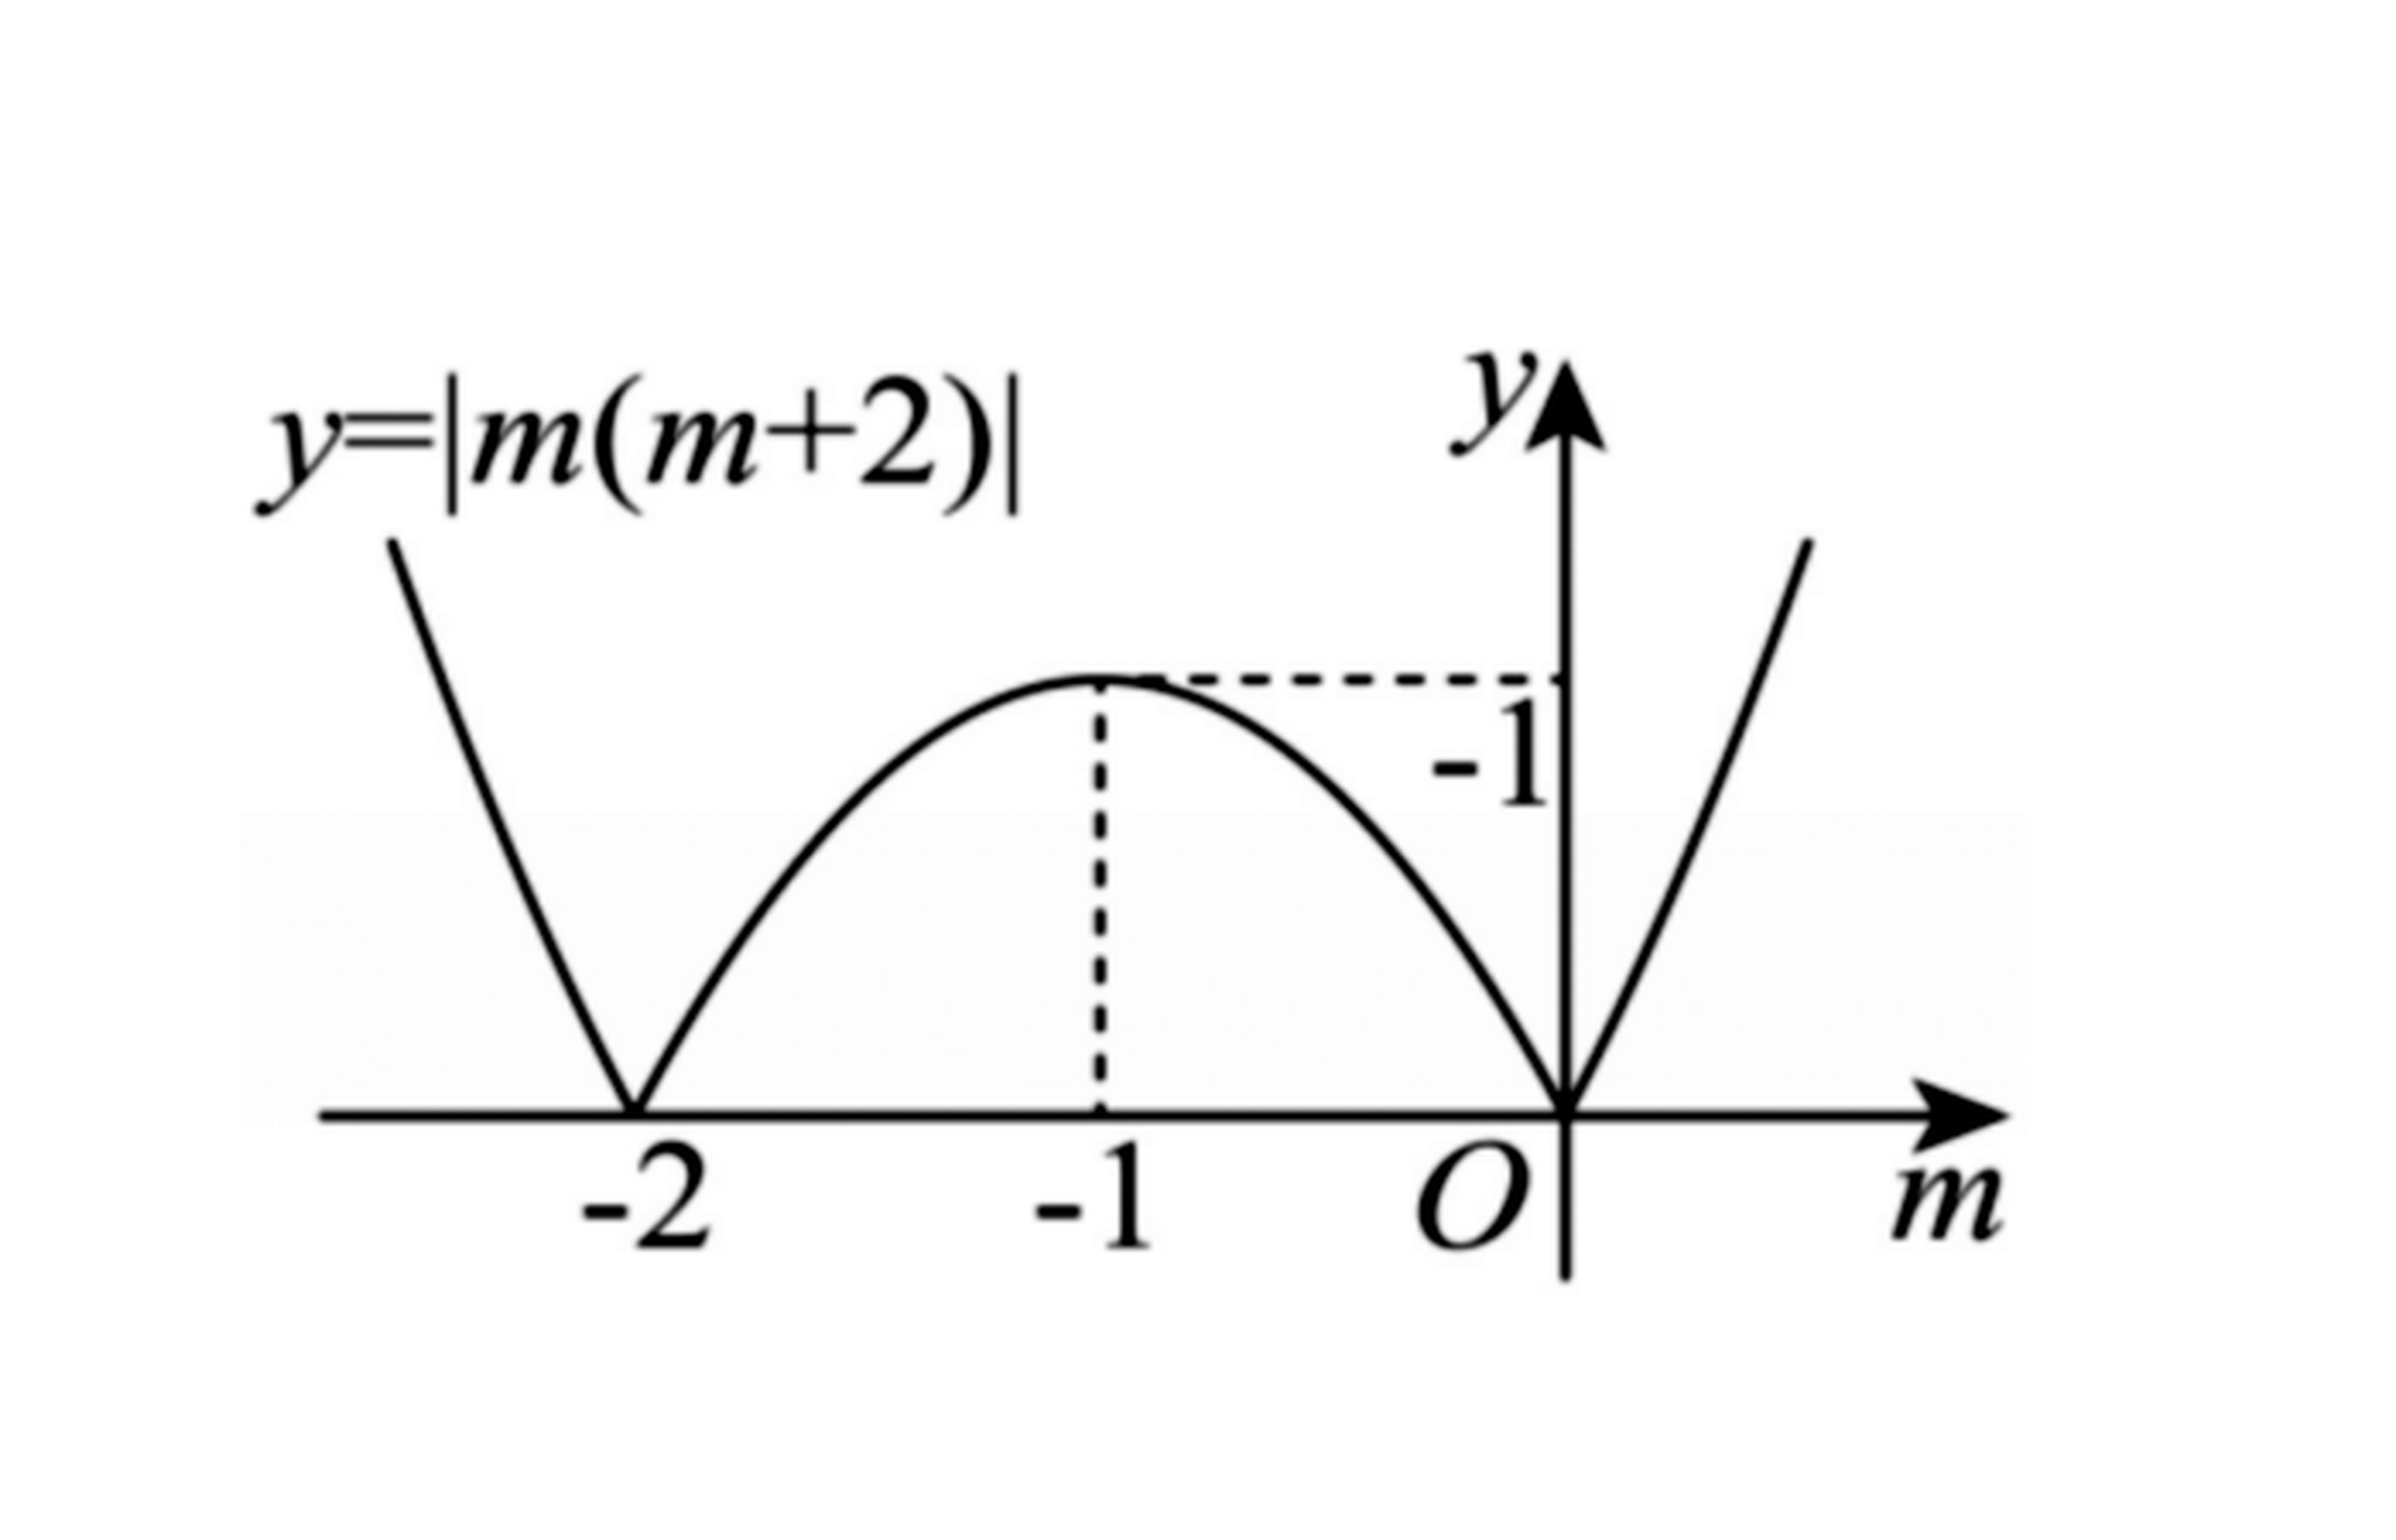
\includegraphics[width=0.46\textwidth]{figures/gao154_fujia2.png}
\end{center}
\step{由图像得 $k\in(0,1)$，}
\step{所以方程 $m^2+2m=k$ 和 $m^2+2m=-k$ 各有两个不同的根，}
\step{其中方程 $m^2+2m-k=0$ 的两根为 $m=-1\pm\sqrt{1+k}$，}
\step{方程 $m^2+2m+k=0$ 的两根为 $m=-1\pm\sqrt{1-k}$，}
\step{所以 $m_1=-1-\sqrt{1+k}$，$m_2=-1-\sqrt{1-k}$，$m_3=-1+\sqrt{1-k}$，$m_4=-1+\sqrt{1+k}$，且 $m_1<m_2<m_3<m_4$，}
\step{由 $m=\log_2 x$，则 $x=2^m$，}
\step{所以 $a=2^{-1-\sqrt{1+k}}$，$b=2^{-1-\sqrt{1-k}}$，$c=2^{-1+\sqrt{1-k}}$，$d=2^{-1+\sqrt{1+k}}$，}
\step{所以 $ad=2^{-1-\sqrt{1+k}}\times2^{-1+\sqrt{1+k}}=2^{(-1-\sqrt{1+k})+(-1+\sqrt{1+k})}=2^{-2}=\dfrac14$，}
\step{$b+c=2^{-1-\sqrt{1-k}}+2^{-1+\sqrt{1-k}}=\dfrac{2^{-\sqrt{1-k}}+2^{\sqrt{1-k}}}{2}$，}
\step{令 $s=\sqrt{1-k}$，其中 $s\in(0,1)$，则 $b+c=\dfrac12\left(2^{-s}+2^s\right)$，}
\step{设函数 $y=2^s+\dfrac1{2^s}$，令 $r=2^s\in(1,2)$，所以 $y=r+\dfrac1r$ 在 $(1,2)$ 上严格增，}
\step{所以函数 $y=2^s+\dfrac1{2^s}$ 在 $(0,1)$ 上严格增，所以 $y=2^s+\dfrac1{2^s}\in\left(2,\dfrac52\right)$，}
\step{所以 $b+c=\dfrac{2^{-s}+2^s}{2}\in\left(1,\dfrac54\right)$，$ad(b+c)=\dfrac{b+c}{4}\in\left(\dfrac14,\dfrac5{16}\right)$，}
\step{所以 $ad(b+c)$ 的取值范围是 $\left(\dfrac14,\dfrac5{16}\right)$，故选 $A$.}
\solend
\fi

\end{enumerate}

\end{document}
